\documentclass[twoside]{book}

% Packages required by doxygen
\usepackage{fixltx2e}
\usepackage{calc}
\usepackage{doxygen}
\usepackage[export]{adjustbox} % also loads graphicx
\usepackage{graphicx}
\usepackage[utf8]{inputenc}
\usepackage{makeidx}
\usepackage{multicol}
\usepackage{multirow}
\PassOptionsToPackage{warn}{textcomp}
\usepackage{textcomp}
\usepackage[nointegrals]{wasysym}
\usepackage[table]{xcolor}

% Font selection
\usepackage[T1]{fontenc}
\usepackage[scaled=.90]{helvet}
\usepackage{courier}
\usepackage{amssymb}
\usepackage{sectsty}
\renewcommand{\familydefault}{\sfdefault}
\allsectionsfont{%
  \fontseries{bc}\selectfont%
  \color{darkgray}%
}
\renewcommand{\DoxyLabelFont}{%
  \fontseries{bc}\selectfont%
  \color{darkgray}%
}
\newcommand{\+}{\discretionary{\mbox{\scriptsize$\hookleftarrow$}}{}{}}

% Page & text layout
\usepackage{geometry}
\geometry{%
  a4paper,%
  top=2.5cm,%
  bottom=2.5cm,%
  left=2.5cm,%
  right=2.5cm%
}
\tolerance=750
\hfuzz=15pt
\hbadness=750
\setlength{\emergencystretch}{15pt}
\setlength{\parindent}{0cm}
\setlength{\parskip}{3ex plus 2ex minus 2ex}
\makeatletter
\renewcommand{\paragraph}{%
  \@startsection{paragraph}{4}{0ex}{-1.0ex}{1.0ex}{%
    \normalfont\normalsize\bfseries\SS@parafont%
  }%
}
\renewcommand{\subparagraph}{%
  \@startsection{subparagraph}{5}{0ex}{-1.0ex}{1.0ex}{%
    \normalfont\normalsize\bfseries\SS@subparafont%
  }%
}
\makeatother

% Headers & footers
\usepackage{fancyhdr}
\pagestyle{fancyplain}
\fancyhead[LE]{\fancyplain{}{\bfseries\thepage}}
\fancyhead[CE]{\fancyplain{}{}}
\fancyhead[RE]{\fancyplain{}{\bfseries\leftmark}}
\fancyhead[LO]{\fancyplain{}{\bfseries\rightmark}}
\fancyhead[CO]{\fancyplain{}{}}
\fancyhead[RO]{\fancyplain{}{\bfseries\thepage}}
\fancyfoot[LE]{\fancyplain{}{}}
\fancyfoot[CE]{\fancyplain{}{}}
\fancyfoot[RE]{\fancyplain{}{\bfseries\scriptsize Generated by Doxygen }}
\fancyfoot[LO]{\fancyplain{}{\bfseries\scriptsize Generated by Doxygen }}
\fancyfoot[CO]{\fancyplain{}{}}
\fancyfoot[RO]{\fancyplain{}{}}
\renewcommand{\footrulewidth}{0.4pt}
\renewcommand{\chaptermark}[1]{%
  \markboth{#1}{}%
}
\renewcommand{\sectionmark}[1]{%
  \markright{\thesection\ #1}%
}

% Indices & bibliography
\usepackage{natbib}
\usepackage[titles]{tocloft}
\setcounter{tocdepth}{3}
\setcounter{secnumdepth}{5}
\makeindex

% Hyperlinks (required, but should be loaded last)
\usepackage{ifpdf}
\ifpdf
  \usepackage[pdftex,pagebackref=true]{hyperref}
\else
  \usepackage[ps2pdf,pagebackref=true]{hyperref}
\fi
\hypersetup{%
  colorlinks=true,%
  linkcolor=blue,%
  citecolor=blue,%
  unicode%
}

% Custom commands
\newcommand{\clearemptydoublepage}{%
  \newpage{\pagestyle{empty}\cleardoublepage}%
}

\usepackage{caption}
\captionsetup{labelsep=space,justification=centering,font={bf},singlelinecheck=off,skip=4pt,position=top}

%===== C O N T E N T S =====

\begin{document}

% Titlepage & ToC
\hypersetup{pageanchor=false,
             bookmarksnumbered=true,
             pdfencoding=unicode
            }
\pagenumbering{alph}
\begin{titlepage}
\vspace*{7cm}
\begin{center}%
{\Large Drawl \\[1ex]\large 0.\+2.\+0 }\\
\vspace*{1cm}
{\large Generated by Doxygen 1.8.13}\\
\end{center}
\end{titlepage}
\clearemptydoublepage
\pagenumbering{roman}
\tableofcontents
\clearemptydoublepage
\pagenumbering{arabic}
\hypersetup{pageanchor=true}

%--- Begin generated contents ---
\chapter{Namespace Index}
\section{Packages}
Here are the packages with brief descriptions (if available)\+:\begin{DoxyCompactList}
\item\contentsline{section}{\hyperlink{namespacecom}{com} }{\pageref{namespacecom}}{}
\item\contentsline{section}{\hyperlink{namespacecom_1_1aarrelaakso}{com.\+aarrelaakso} }{\pageref{namespacecom_1_1aarrelaakso}}{}
\item\contentsline{section}{\hyperlink{namespacecom_1_1aarrelaakso_1_1drawl}{com.\+aarrelaakso.\+drawl} }{\pageref{namespacecom_1_1aarrelaakso_1_1drawl}}{}
\item\contentsline{section}{\hyperlink{namespacecom_1_1aarrelaakso_1_1drawl_1_1examples}{com.\+aarrelaakso.\+drawl.\+examples} }{\pageref{namespacecom_1_1aarrelaakso_1_1drawl_1_1examples}}{}
\end{DoxyCompactList}

\chapter{Hierarchical Index}
\section{Class Hierarchy}
This inheritance list is sorted roughly, but not completely, alphabetically\+:\begin{DoxyCompactList}
\item Comparable\begin{DoxyCompactList}
\item \contentsline{section}{com.\+aarrelaakso.\+drawl.\+Sisu\+Big\+Decimal}{\pageref{classcom_1_1aarrelaakso_1_1drawl_1_1_sisu_big_decimal}}{}
\end{DoxyCompactList}
\item \contentsline{section}{com.\+aarrelaakso.\+drawl.\+Constraint\+Type}{\pageref{enumcom_1_1aarrelaakso_1_1drawl_1_1_constraint_type}}{}
\item \contentsline{section}{com.\+aarrelaakso.\+drawl.\+Drawing}{\pageref{classcom_1_1aarrelaakso_1_1drawl_1_1_drawing}}{}
\item \contentsline{section}{com.\+aarrelaakso.\+drawl.\+Logging\+Config}{\pageref{classcom_1_1aarrelaakso_1_1drawl_1_1_logging_config}}{}
\item \contentsline{section}{com.\+aarrelaakso.\+drawl.\+Shape}{\pageref{classcom_1_1aarrelaakso_1_1drawl_1_1_shape}}{}
\begin{DoxyCompactList}
\item \contentsline{section}{com.\+aarrelaakso.\+drawl.\+Circle}{\pageref{classcom_1_1aarrelaakso_1_1drawl_1_1_circle}}{}
\item \contentsline{section}{com.\+aarrelaakso.\+drawl.\+Rectangle}{\pageref{classcom_1_1aarrelaakso_1_1drawl_1_1_rectangle}}{}
\item \contentsline{section}{com.\+aarrelaakso.\+drawl.\+Text}{\pageref{classcom_1_1aarrelaakso_1_1drawl_1_1_text}}{}
\end{DoxyCompactList}
\item \contentsline{section}{com.\+aarrelaakso.\+drawl.\+Sisu\+Big\+Decimal\+Remainder\+Pair}{\pageref{classcom_1_1aarrelaakso_1_1drawl_1_1_sisu_big_decimal_remainder_pair}}{}
\item \contentsline{section}{com.\+aarrelaakso.\+drawl.\+S\+VG}{\pageref{classcom_1_1aarrelaakso_1_1drawl_1_1_s_v_g}}{}
\item \contentsline{section}{com.\+aarrelaakso.\+drawl.\+examples.\+Text\+Example}{\pageref{classcom_1_1aarrelaakso_1_1drawl_1_1examples_1_1_text_example}}{}
\item \contentsline{section}{com.\+aarrelaakso.\+drawl.\+examples.\+Three\+Circles\+Horizontal}{\pageref{classcom_1_1aarrelaakso_1_1drawl_1_1examples_1_1_three_circles_horizontal}}{}
\item \contentsline{section}{com.\+aarrelaakso.\+drawl.\+examples.\+Three\+Circles\+Vertical}{\pageref{classcom_1_1aarrelaakso_1_1drawl_1_1examples_1_1_three_circles_vertical}}{}
\end{DoxyCompactList}

\chapter{Class Index}
\section{Class List}
Here are the classes, structs, unions and interfaces with brief descriptions\+:\begin{DoxyCompactList}
\item\contentsline{section}{\hyperlink{classcom_1_1aarrelaakso_1_1drawl_1_1_arrowhead}{com.\+aarrelaakso.\+drawl.\+Arrowhead} \\*Represents heads or tails on the ends of Lines }{\pageref{classcom_1_1aarrelaakso_1_1drawl_1_1_arrowhead}}{}
\item\contentsline{section}{\hyperlink{classcom_1_1aarrelaakso_1_1drawl_1_1examples_1_1_arrowhead_example}{com.\+aarrelaakso.\+drawl.\+examples.\+Arrowhead\+Example} }{\pageref{classcom_1_1aarrelaakso_1_1drawl_1_1examples_1_1_arrowhead_example}}{}
\item\contentsline{section}{\hyperlink{classcom_1_1aarrelaakso_1_1drawl_1_1_circle}{com.\+aarrelaakso.\+drawl.\+Circle} \\*Represents circles }{\pageref{classcom_1_1aarrelaakso_1_1drawl_1_1_circle}}{}
\item\contentsline{section}{\hyperlink{classcom_1_1aarrelaakso_1_1drawl_1_1_drawing}{com.\+aarrelaakso.\+drawl.\+Drawing} \\*Represents drawings }{\pageref{classcom_1_1aarrelaakso_1_1drawl_1_1_drawing}}{}
\item\contentsline{section}{\hyperlink{classcom_1_1aarrelaakso_1_1drawl_1_1_drawl_number}{com.\+aarrelaakso.\+drawl.\+Drawl\+Number} \\*Class for mathematical operations with Double values that have a similar A\+PI to that of the Big\+Decimal class }{\pageref{classcom_1_1aarrelaakso_1_1drawl_1_1_drawl_number}}{}
\item\contentsline{section}{\hyperlink{classcom_1_1aarrelaakso_1_1drawl_1_1_drawl_number_remainder_pair}{com.\+aarrelaakso.\+drawl.\+Drawl\+Number\+Remainder\+Pair} \\*Pair of the arbitrary number and remainder }{\pageref{classcom_1_1aarrelaakso_1_1drawl_1_1_drawl_number_remainder_pair}}{}
\item\contentsline{section}{\hyperlink{classcom_1_1aarrelaakso_1_1drawl_1_1_line}{com.\+aarrelaakso.\+drawl.\+Line} \\*Represents lines }{\pageref{classcom_1_1aarrelaakso_1_1drawl_1_1_line}}{}
\item\contentsline{section}{\hyperlink{classcom_1_1aarrelaakso_1_1drawl_1_1examples_1_1_line_example}{com.\+aarrelaakso.\+drawl.\+examples.\+Line\+Example} \\*Example of using Drawl to draw a line between two shapes }{\pageref{classcom_1_1aarrelaakso_1_1drawl_1_1examples_1_1_line_example}}{}
\item\contentsline{section}{\hyperlink{classcom_1_1aarrelaakso_1_1drawl_1_1_logging_config}{com.\+aarrelaakso.\+drawl.\+Logging\+Config} \\*Manages logging configuration }{\pageref{classcom_1_1aarrelaakso_1_1drawl_1_1_logging_config}}{}
\item\contentsline{section}{\hyperlink{classcom_1_1aarrelaakso_1_1drawl_1_1_measure}{com.\+aarrelaakso.\+drawl.\+Measure} \\*Defines a public \hyperlink{classcom_1_1aarrelaakso_1_1drawl_1_1_measure}{Measure} class to represent measures on the diagram without exposing internal numerical measurements to the user }{\pageref{classcom_1_1aarrelaakso_1_1drawl_1_1_measure}}{}
\item\contentsline{section}{\hyperlink{classcom_1_1aarrelaakso_1_1drawl_1_1examples_1_1_nonadjacency}{com.\+aarrelaakso.\+drawl.\+examples.\+Nonadjacency} \\*Example of using Drawl to draw shapes separated by some distance }{\pageref{classcom_1_1aarrelaakso_1_1drawl_1_1examples_1_1_nonadjacency}}{}
\item\contentsline{section}{\hyperlink{interfacecom_1_1aarrelaakso_1_1drawl_1_1_number}{com.\+aarrelaakso.\+drawl.\+Number} \\*Class for mathematical operations with Double values that have a similar A\+PI to that of the Big\+Decimal class }{\pageref{interfacecom_1_1aarrelaakso_1_1drawl_1_1_number}}{}
\item\contentsline{section}{\hyperlink{classcom_1_1aarrelaakso_1_1drawl_1_1_point}{com.\+aarrelaakso.\+drawl.\+Point} \\*Represents a point on the drawing canvas }{\pageref{classcom_1_1aarrelaakso_1_1drawl_1_1_point}}{}
\item\contentsline{section}{\hyperlink{classcom_1_1aarrelaakso_1_1drawl_1_1examples_1_1_policy_priorities}{com.\+aarrelaakso.\+drawl.\+examples.\+Policy\+Priorities} }{\pageref{classcom_1_1aarrelaakso_1_1drawl_1_1examples_1_1_policy_priorities}}{}
\item\contentsline{section}{\hyperlink{classcom_1_1aarrelaakso_1_1drawl_1_1_rectangle}{com.\+aarrelaakso.\+drawl.\+Rectangle} \\*Represents rectangles }{\pageref{classcom_1_1aarrelaakso_1_1drawl_1_1_rectangle}}{}
\item\contentsline{section}{\hyperlink{classcom_1_1aarrelaakso_1_1drawl_1_1examples_1_1_shaded_rectangles}{com.\+aarrelaakso.\+drawl.\+examples.\+Shaded\+Rectangles} \\*Example of using Drawl to draw a series of shaded rectangles }{\pageref{classcom_1_1aarrelaakso_1_1drawl_1_1examples_1_1_shaded_rectangles}}{}
\item\contentsline{section}{\hyperlink{classcom_1_1aarrelaakso_1_1drawl_1_1_shape}{com.\+aarrelaakso.\+drawl.\+Shape} \\*Abstract class represents shapes such as circles, rectangles, and lines }{\pageref{classcom_1_1aarrelaakso_1_1drawl_1_1_shape}}{}
\item\contentsline{section}{\hyperlink{classcom_1_1aarrelaakso_1_1drawl_1_1_shape_explicit}{com.\+aarrelaakso.\+drawl.\+Shape\+Explicit} }{\pageref{classcom_1_1aarrelaakso_1_1drawl_1_1_shape_explicit}}{}
\item\contentsline{section}{\hyperlink{classcom_1_1aarrelaakso_1_1drawl_1_1_sisu_number}{com.\+aarrelaakso.\+drawl.\+Sisu\+Number} \\*Class for mathematical operations with Big\+Decimal values that are not provided by the Big\+Decimal class itself }{\pageref{classcom_1_1aarrelaakso_1_1drawl_1_1_sisu_number}}{}
\item\contentsline{section}{\hyperlink{classcom_1_1aarrelaakso_1_1drawl_1_1_sisu_number_remainder_pair}{com.\+aarrelaakso.\+drawl.\+Sisu\+Number\+Remainder\+Pair} \\*Pair of the arbitrary number and remainder }{\pageref{classcom_1_1aarrelaakso_1_1drawl_1_1_sisu_number_remainder_pair}}{}
\item\contentsline{section}{\hyperlink{classcom_1_1aarrelaakso_1_1drawl_1_1_s_v_g}{com.\+aarrelaakso.\+drawl.\+S\+VG} \\*Helper class for generating \hyperlink{classcom_1_1aarrelaakso_1_1drawl_1_1_s_v_g}{S\+VG} }{\pageref{classcom_1_1aarrelaakso_1_1drawl_1_1_s_v_g}}{}
\item\contentsline{section}{\hyperlink{classcom_1_1aarrelaakso_1_1drawl_1_1_text}{com.\+aarrelaakso.\+drawl.\+Text} \\*Represents text on a drawing }{\pageref{classcom_1_1aarrelaakso_1_1drawl_1_1_text}}{}
\item\contentsline{section}{\hyperlink{classcom_1_1aarrelaakso_1_1drawl_1_1examples_1_1_text_example}{com.\+aarrelaakso.\+drawl.\+examples.\+Text\+Example} \\*Example of using Drawl to draw text }{\pageref{classcom_1_1aarrelaakso_1_1drawl_1_1examples_1_1_text_example}}{}
\item\contentsline{section}{\hyperlink{classcom_1_1aarrelaakso_1_1drawl_1_1examples_1_1_three_circles_horizontal}{com.\+aarrelaakso.\+drawl.\+examples.\+Three\+Circles\+Horizontal} \\*Example of using Drawl to draw three adjacent circles oriented horizontally }{\pageref{classcom_1_1aarrelaakso_1_1drawl_1_1examples_1_1_three_circles_horizontal}}{}
\item\contentsline{section}{\hyperlink{classcom_1_1aarrelaakso_1_1drawl_1_1examples_1_1_three_circles_vertical}{com.\+aarrelaakso.\+drawl.\+examples.\+Three\+Circles\+Vertical} \\*Example of using Drawl to draw three adjacent circles oriented vertically }{\pageref{classcom_1_1aarrelaakso_1_1drawl_1_1examples_1_1_three_circles_vertical}}{}
\item\contentsline{section}{\hyperlink{enumcom_1_1aarrelaakso_1_1drawl_1_1_arrowhead_1_1_type}{com.\+aarrelaakso.\+drawl.\+Arrowhead.\+Type} \\*Defines the different types of arrowheads that are available }{\pageref{enumcom_1_1aarrelaakso_1_1drawl_1_1_arrowhead_1_1_type}}{}
\end{DoxyCompactList}

\chapter{File Index}
\section{File List}
Here is a list of all files with brief descriptions\+:\begin{DoxyCompactList}
\item\contentsline{section}{/mnt/d/\+One\+Drive/\+Documents/src/drawl/src/main/java/com/aarrelaakso/drawl/\hyperlink{_circle_8java}{Circle.\+java} }{\pageref{_circle_8java}}{}
\item\contentsline{section}{/mnt/d/\+One\+Drive/\+Documents/src/drawl/src/main/java/com/aarrelaakso/drawl/\hyperlink{_constraint_type_8java}{Constraint\+Type.\+java} }{\pageref{_constraint_type_8java}}{}
\item\contentsline{section}{/mnt/d/\+One\+Drive/\+Documents/src/drawl/src/main/java/com/aarrelaakso/drawl/\hyperlink{_drawing_8java}{Drawing.\+java} }{\pageref{_drawing_8java}}{}
\item\contentsline{section}{/mnt/d/\+One\+Drive/\+Documents/src/drawl/src/main/java/com/aarrelaakso/drawl/\hyperlink{_logging_config_8java}{Logging\+Config.\+java} }{\pageref{_logging_config_8java}}{}
\item\contentsline{section}{/mnt/d/\+One\+Drive/\+Documents/src/drawl/src/main/java/com/aarrelaakso/drawl/\hyperlink{_rectangle_8java}{Rectangle.\+java} }{\pageref{_rectangle_8java}}{}
\item\contentsline{section}{/mnt/d/\+One\+Drive/\+Documents/src/drawl/src/main/java/com/aarrelaakso/drawl/\hyperlink{_shape_8java}{Shape.\+java} }{\pageref{_shape_8java}}{}
\item\contentsline{section}{/mnt/d/\+One\+Drive/\+Documents/src/drawl/src/main/java/com/aarrelaakso/drawl/\hyperlink{_sisu_big_decimal_8java}{Sisu\+Big\+Decimal.\+java} }{\pageref{_sisu_big_decimal_8java}}{}
\item\contentsline{section}{/mnt/d/\+One\+Drive/\+Documents/src/drawl/src/main/java/com/aarrelaakso/drawl/\hyperlink{_sisu_big_decimal_remainder_pair_8java}{Sisu\+Big\+Decimal\+Remainder\+Pair.\+java} }{\pageref{_sisu_big_decimal_remainder_pair_8java}}{}
\item\contentsline{section}{/mnt/d/\+One\+Drive/\+Documents/src/drawl/src/main/java/com/aarrelaakso/drawl/\hyperlink{_s_v_g_8java}{S\+V\+G.\+java} }{\pageref{_s_v_g_8java}}{}
\item\contentsline{section}{/mnt/d/\+One\+Drive/\+Documents/src/drawl/src/main/java/com/aarrelaakso/drawl/\hyperlink{_text_8java}{Text.\+java} }{\pageref{_text_8java}}{}
\item\contentsline{section}{/mnt/d/\+One\+Drive/\+Documents/src/drawl/src/main/java/com/aarrelaakso/drawl/examples/\hyperlink{_text_example_8java}{Text\+Example.\+java} }{\pageref{_text_example_8java}}{}
\item\contentsline{section}{/mnt/d/\+One\+Drive/\+Documents/src/drawl/src/main/java/com/aarrelaakso/drawl/examples/\hyperlink{_three_circles_horizontal_8java}{Three\+Circles\+Horizontal.\+java} }{\pageref{_three_circles_horizontal_8java}}{}
\item\contentsline{section}{/mnt/d/\+One\+Drive/\+Documents/src/drawl/src/main/java/com/aarrelaakso/drawl/examples/\hyperlink{_three_circles_vertical_8java}{Three\+Circles\+Vertical.\+java} }{\pageref{_three_circles_vertical_8java}}{}
\end{DoxyCompactList}

\chapter{Namespace Documentation}
\hypertarget{namespacecom}{}\section{Package com}
\label{namespacecom}\index{com@{com}}
\subsection*{Packages}
\begin{DoxyCompactItemize}
\item 
package \hyperlink{namespacecom_1_1aarrelaakso}{aarrelaakso}
\end{DoxyCompactItemize}

\hypertarget{namespacecom_1_1aarrelaakso}{}\section{Package com.\+aarrelaakso}
\label{namespacecom_1_1aarrelaakso}\index{com.\+aarrelaakso@{com.\+aarrelaakso}}
\subsection*{Packages}
\begin{DoxyCompactItemize}
\item 
package \hyperlink{namespacecom_1_1aarrelaakso_1_1drawl}{drawl}
\end{DoxyCompactItemize}

\hypertarget{namespacecom_1_1aarrelaakso_1_1drawl}{}\section{Package com.\+aarrelaakso.\+drawl}
\label{namespacecom_1_1aarrelaakso_1_1drawl}\index{com.\+aarrelaakso.\+drawl@{com.\+aarrelaakso.\+drawl}}
\subsection*{Packages}
\begin{DoxyCompactItemize}
\item 
package \hyperlink{namespacecom_1_1aarrelaakso_1_1drawl_1_1examples}{examples}
\end{DoxyCompactItemize}
\subsection*{Classes}
\begin{DoxyCompactItemize}
\item 
class \hyperlink{classcom_1_1aarrelaakso_1_1drawl_1_1_circle}{Circle}
\item 
enum \hyperlink{enumcom_1_1aarrelaakso_1_1drawl_1_1_constraint_type}{Constraint\+Type}
\item 
class \hyperlink{classcom_1_1aarrelaakso_1_1drawl_1_1_drawing}{Drawing}
\item 
class \hyperlink{classcom_1_1aarrelaakso_1_1drawl_1_1_logging_config}{Logging\+Config}
\item 
class \hyperlink{classcom_1_1aarrelaakso_1_1drawl_1_1_rectangle}{Rectangle}
\item 
class \hyperlink{classcom_1_1aarrelaakso_1_1drawl_1_1_shape}{Shape}
\item 
class \hyperlink{classcom_1_1aarrelaakso_1_1drawl_1_1_sisu_big_decimal}{Sisu\+Big\+Decimal}
\item 
class \hyperlink{classcom_1_1aarrelaakso_1_1drawl_1_1_sisu_big_decimal_remainder_pair}{Sisu\+Big\+Decimal\+Remainder\+Pair}
\item 
class \hyperlink{classcom_1_1aarrelaakso_1_1drawl_1_1_s_v_g}{S\+VG}
\item 
class \hyperlink{classcom_1_1aarrelaakso_1_1drawl_1_1_text}{Text}
\end{DoxyCompactItemize}

\hypertarget{namespacecom_1_1aarrelaakso_1_1drawl_1_1examples}{}\section{Package com.\+aarrelaakso.\+drawl.\+examples}
\label{namespacecom_1_1aarrelaakso_1_1drawl_1_1examples}\index{com.\+aarrelaakso.\+drawl.\+examples@{com.\+aarrelaakso.\+drawl.\+examples}}
\subsection*{Classes}
\begin{DoxyCompactItemize}
\item 
class \hyperlink{classcom_1_1aarrelaakso_1_1drawl_1_1examples_1_1_line_example}{Line\+Example}
\item 
class \hyperlink{classcom_1_1aarrelaakso_1_1drawl_1_1examples_1_1_nonadjacency}{Nonadjacency}
\item 
class \hyperlink{classcom_1_1aarrelaakso_1_1drawl_1_1examples_1_1_policy_priorities}{Policy\+Priorities}
\item 
class \hyperlink{classcom_1_1aarrelaakso_1_1drawl_1_1examples_1_1_shaded_rectangles}{Shaded\+Rectangles}
\item 
class \hyperlink{classcom_1_1aarrelaakso_1_1drawl_1_1examples_1_1_text_example}{Text\+Example}
\item 
class \hyperlink{classcom_1_1aarrelaakso_1_1drawl_1_1examples_1_1_three_circles_horizontal}{Three\+Circles\+Horizontal}
\item 
class \hyperlink{classcom_1_1aarrelaakso_1_1drawl_1_1examples_1_1_three_circles_vertical}{Three\+Circles\+Vertical}
\end{DoxyCompactItemize}

\chapter{Class Documentation}
\hypertarget{classcom_1_1aarrelaakso_1_1drawl_1_1_arrowhead}{}\section{com.\+aarrelaakso.\+drawl.\+Arrowhead Class Reference}
\label{classcom_1_1aarrelaakso_1_1drawl_1_1_arrowhead}\index{com.\+aarrelaakso.\+drawl.\+Arrowhead@{com.\+aarrelaakso.\+drawl.\+Arrowhead}}


Represents heads or tails on the ends of \hyperlink{classcom_1_1aarrelaakso_1_1drawl_1_1_line}{Line}.  




Collaboration diagram for com.\+aarrelaakso.\+drawl.\+Arrowhead\+:
\nopagebreak
\begin{figure}[H]
\begin{center}
\leavevmode
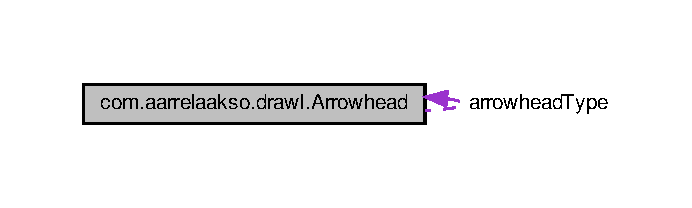
\includegraphics[width=332pt]{d2/db3/classcom_1_1aarrelaakso_1_1drawl_1_1_arrowhead__coll__graph}
\end{center}
\end{figure}
\subsection*{Classes}
\begin{DoxyCompactItemize}
\item 
enum \hyperlink{enumcom_1_1aarrelaakso_1_1drawl_1_1_arrowhead_1_1_type}{Type}
\end{DoxyCompactItemize}
\subsection*{Public Member Functions}
\begin{DoxyCompactItemize}
\item 
\hyperlink{classcom_1_1aarrelaakso_1_1drawl_1_1_arrowhead_a866fb3900ad67226bad5962031cc7817}{Arrowhead} ()
\begin{DoxyCompactList}\small\item\em Constructs a default arrowhead. \end{DoxyCompactList}\item 
\hyperlink{classcom_1_1aarrelaakso_1_1drawl_1_1_arrowhead_a43464dd3355fda0d6e295d4282433828}{Arrowhead} (@Not\+Null Arrowhead.\+Type type)
\begin{DoxyCompactList}\small\item\em Constructs an arrowhead of a particular type. \end{DoxyCompactList}\end{DoxyCompactItemize}
\subsection*{Protected Member Functions}
\begin{DoxyCompactItemize}
\item 
String \hyperlink{classcom_1_1aarrelaakso_1_1drawl_1_1_arrowhead_a0094c4f48945d782b7e474b15ef06561}{get\+S\+V\+G\+Def} ()
\end{DoxyCompactItemize}
\subsection*{Private Attributes}
\begin{DoxyCompactItemize}
\item 
Arrowhead.\+Type \hyperlink{classcom_1_1aarrelaakso_1_1drawl_1_1_arrowhead_a72183bdf6672377d73b2d9810b6d0ed7}{arrowhead\+Type} = \hyperlink{enumcom_1_1aarrelaakso_1_1drawl_1_1_arrowhead_1_1_type_ae4c70d3cd0853637fba791f2bb29cd8e}{Type.\+D\+E\+F\+A\+U\+LT}
\end{DoxyCompactItemize}


\subsection{Detailed Description}
Represents heads or tails on the ends of \hyperlink{classcom_1_1aarrelaakso_1_1drawl_1_1_line}{Line}. 

\subsection{Constructor \& Destructor Documentation}
\mbox{\Hypertarget{classcom_1_1aarrelaakso_1_1drawl_1_1_arrowhead_a866fb3900ad67226bad5962031cc7817}\label{classcom_1_1aarrelaakso_1_1drawl_1_1_arrowhead_a866fb3900ad67226bad5962031cc7817}} 
\index{com\+::aarrelaakso\+::drawl\+::\+Arrowhead@{com\+::aarrelaakso\+::drawl\+::\+Arrowhead}!Arrowhead@{Arrowhead}}
\index{Arrowhead@{Arrowhead}!com\+::aarrelaakso\+::drawl\+::\+Arrowhead@{com\+::aarrelaakso\+::drawl\+::\+Arrowhead}}
\subsubsection{\texorpdfstring{Arrowhead()}{Arrowhead()}\hspace{0.1cm}{\footnotesize\ttfamily [1/2]}}
{\footnotesize\ttfamily com.\+aarrelaakso.\+drawl.\+Arrowhead.\+Arrowhead (\begin{DoxyParamCaption}{ }\end{DoxyParamCaption})}



Constructs a default arrowhead. 

\mbox{\Hypertarget{classcom_1_1aarrelaakso_1_1drawl_1_1_arrowhead_a43464dd3355fda0d6e295d4282433828}\label{classcom_1_1aarrelaakso_1_1drawl_1_1_arrowhead_a43464dd3355fda0d6e295d4282433828}} 
\index{com\+::aarrelaakso\+::drawl\+::\+Arrowhead@{com\+::aarrelaakso\+::drawl\+::\+Arrowhead}!Arrowhead@{Arrowhead}}
\index{Arrowhead@{Arrowhead}!com\+::aarrelaakso\+::drawl\+::\+Arrowhead@{com\+::aarrelaakso\+::drawl\+::\+Arrowhead}}
\subsubsection{\texorpdfstring{Arrowhead()}{Arrowhead()}\hspace{0.1cm}{\footnotesize\ttfamily [2/2]}}
{\footnotesize\ttfamily com.\+aarrelaakso.\+drawl.\+Arrowhead.\+Arrowhead (\begin{DoxyParamCaption}\item[{@Not\+Null Arrowhead.\+Type}]{type }\end{DoxyParamCaption})}



Constructs an arrowhead of a particular type. 


\begin{DoxyParams}{Parameters}
{\em type} & \\
\hline
\end{DoxyParams}


\subsection{Member Function Documentation}
\mbox{\Hypertarget{classcom_1_1aarrelaakso_1_1drawl_1_1_arrowhead_a0094c4f48945d782b7e474b15ef06561}\label{classcom_1_1aarrelaakso_1_1drawl_1_1_arrowhead_a0094c4f48945d782b7e474b15ef06561}} 
\index{com\+::aarrelaakso\+::drawl\+::\+Arrowhead@{com\+::aarrelaakso\+::drawl\+::\+Arrowhead}!get\+S\+V\+G\+Def@{get\+S\+V\+G\+Def}}
\index{get\+S\+V\+G\+Def@{get\+S\+V\+G\+Def}!com\+::aarrelaakso\+::drawl\+::\+Arrowhead@{com\+::aarrelaakso\+::drawl\+::\+Arrowhead}}
\subsubsection{\texorpdfstring{get\+S\+V\+G\+Def()}{getSVGDef()}}
{\footnotesize\ttfamily String com.\+aarrelaakso.\+drawl.\+Arrowhead.\+get\+S\+V\+G\+Def (\begin{DoxyParamCaption}{ }\end{DoxyParamCaption})\hspace{0.3cm}{\ttfamily [protected]}}



\subsection{Member Data Documentation}
\mbox{\Hypertarget{classcom_1_1aarrelaakso_1_1drawl_1_1_arrowhead_a72183bdf6672377d73b2d9810b6d0ed7}\label{classcom_1_1aarrelaakso_1_1drawl_1_1_arrowhead_a72183bdf6672377d73b2d9810b6d0ed7}} 
\index{com\+::aarrelaakso\+::drawl\+::\+Arrowhead@{com\+::aarrelaakso\+::drawl\+::\+Arrowhead}!arrowhead\+Type@{arrowhead\+Type}}
\index{arrowhead\+Type@{arrowhead\+Type}!com\+::aarrelaakso\+::drawl\+::\+Arrowhead@{com\+::aarrelaakso\+::drawl\+::\+Arrowhead}}
\subsubsection{\texorpdfstring{arrowhead\+Type}{arrowheadType}}
{\footnotesize\ttfamily Arrowhead.\+Type com.\+aarrelaakso.\+drawl.\+Arrowhead.\+arrowhead\+Type = \hyperlink{enumcom_1_1aarrelaakso_1_1drawl_1_1_arrowhead_1_1_type_ae4c70d3cd0853637fba791f2bb29cd8e}{Type.\+D\+E\+F\+A\+U\+LT}\hspace{0.3cm}{\ttfamily [private]}}



The documentation for this class was generated from the following file\+:\begin{DoxyCompactItemize}
\item 
/mnt/d/\+One\+Drive/\+Documents/src/drawl/src/main/java/com/aarrelaakso/drawl/\hyperlink{_arrowhead_8java}{Arrowhead.\+java}\end{DoxyCompactItemize}

\hypertarget{classcom_1_1aarrelaakso_1_1drawl_1_1examples_1_1_arrowhead_example}{}\section{com.\+aarrelaakso.\+drawl.\+examples.\+Arrowhead\+Example Class Reference}
\label{classcom_1_1aarrelaakso_1_1drawl_1_1examples_1_1_arrowhead_example}\index{com.\+aarrelaakso.\+drawl.\+examples.\+Arrowhead\+Example@{com.\+aarrelaakso.\+drawl.\+examples.\+Arrowhead\+Example}}
\subsection*{Static Public Member Functions}
\begin{DoxyCompactItemize}
\item 
static void \hyperlink{classcom_1_1aarrelaakso_1_1drawl_1_1examples_1_1_arrowhead_example_ad77c13fdb08b2be4a9517048463ba379}{main} (final String\mbox{[}$\,$\mbox{]} args)  throws I\+O\+Exception 
\end{DoxyCompactItemize}


\subsection{Member Function Documentation}
\mbox{\Hypertarget{classcom_1_1aarrelaakso_1_1drawl_1_1examples_1_1_arrowhead_example_ad77c13fdb08b2be4a9517048463ba379}\label{classcom_1_1aarrelaakso_1_1drawl_1_1examples_1_1_arrowhead_example_ad77c13fdb08b2be4a9517048463ba379}} 
\index{com\+::aarrelaakso\+::drawl\+::examples\+::\+Arrowhead\+Example@{com\+::aarrelaakso\+::drawl\+::examples\+::\+Arrowhead\+Example}!main@{main}}
\index{main@{main}!com\+::aarrelaakso\+::drawl\+::examples\+::\+Arrowhead\+Example@{com\+::aarrelaakso\+::drawl\+::examples\+::\+Arrowhead\+Example}}
\subsubsection{\texorpdfstring{main()}{main()}}
{\footnotesize\ttfamily static void com.\+aarrelaakso.\+drawl.\+examples.\+Arrowhead\+Example.\+main (\begin{DoxyParamCaption}\item[{final String \mbox{[}$\,$\mbox{]}}]{args }\end{DoxyParamCaption}) throws I\+O\+Exception\hspace{0.3cm}{\ttfamily [static]}}



The documentation for this class was generated from the following file\+:\begin{DoxyCompactItemize}
\item 
/mnt/d/\+One\+Drive/\+Documents/src/drawl/src/main/java/com/aarrelaakso/drawl/examples/\hyperlink{_arrowhead_example_8java}{Arrowhead\+Example.\+java}\end{DoxyCompactItemize}

\hypertarget{classcom_1_1aarrelaakso_1_1drawl_1_1_circle}{}\section{com.\+aarrelaakso.\+drawl.\+Circle Class Reference}
\label{classcom_1_1aarrelaakso_1_1drawl_1_1_circle}\index{com.\+aarrelaakso.\+drawl.\+Circle@{com.\+aarrelaakso.\+drawl.\+Circle}}


Represents circles.  




Inheritance diagram for com.\+aarrelaakso.\+drawl.\+Circle\+:\nopagebreak
\begin{figure}[H]
\begin{center}
\leavevmode
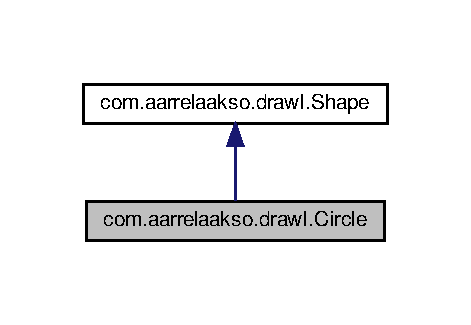
\includegraphics[width=226pt]{dd/d1c/classcom_1_1aarrelaakso_1_1drawl_1_1_circle__inherit__graph}
\end{center}
\end{figure}


Collaboration diagram for com.\+aarrelaakso.\+drawl.\+Circle\+:
\nopagebreak
\begin{figure}[H]
\begin{center}
\leavevmode
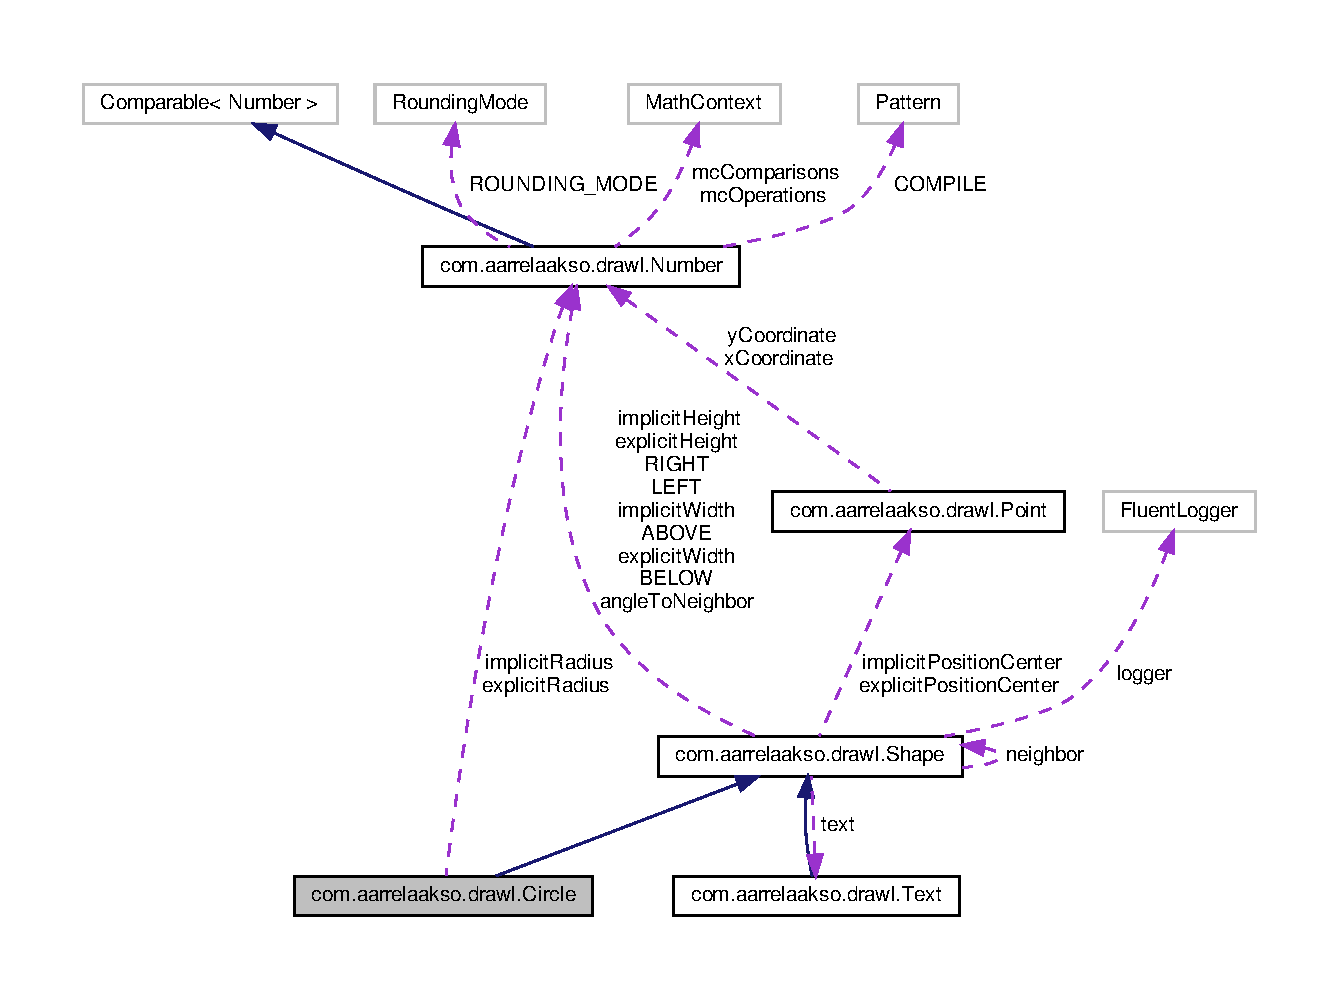
\includegraphics[width=350pt]{de/d25/classcom_1_1aarrelaakso_1_1drawl_1_1_circle__coll__graph}
\end{center}
\end{figure}
\subsection*{Public Member Functions}
\begin{DoxyCompactItemize}
\item 
\hyperlink{classcom_1_1aarrelaakso_1_1drawl_1_1_circle_a18cd01a953d72d49941bc8211f50d268}{Circle} ()
\begin{DoxyCompactList}\small\item\em Construct a circle with a default implicit radius. \end{DoxyCompactList}\item 
String \hyperlink{classcom_1_1aarrelaakso_1_1drawl_1_1_circle_adc826cc2d93eb4e78318035c86d00f03}{get\+S\+VG} ()
\begin{DoxyCompactList}\small\item\em Get \hyperlink{classcom_1_1aarrelaakso_1_1drawl_1_1_s_v_g}{S\+VG} representing this \hyperlink{classcom_1_1aarrelaakso_1_1drawl_1_1_circle}{Circle}. \end{DoxyCompactList}\item 
void \hyperlink{classcom_1_1aarrelaakso_1_1drawl_1_1_shape_af6fea9610721de462c18ee640043aba7}{add\+Text} (@Nullable final \hyperlink{classcom_1_1aarrelaakso_1_1drawl_1_1_text}{Text} \hyperlink{classcom_1_1aarrelaakso_1_1drawl_1_1_shape_ab54afc2d95d3447532f5ecf3fec3faa8}{text})
\begin{DoxyCompactList}\small\item\em Adds \hyperlink{classcom_1_1aarrelaakso_1_1drawl_1_1_text}{Text} inside this \hyperlink{classcom_1_1aarrelaakso_1_1drawl_1_1_shape}{Shape}. \end{DoxyCompactList}\item 
\hyperlink{classcom_1_1aarrelaakso_1_1drawl_1_1_shape}{Shape} \hyperlink{classcom_1_1aarrelaakso_1_1drawl_1_1_shape_acebea2aa57031322323c9bf50ee447db}{get\+Above} ()
\begin{DoxyCompactList}\small\item\em Gets this \hyperlink{classcom_1_1aarrelaakso_1_1drawl_1_1_shape}{Shape}\textquotesingle{}s neighbor above (this \hyperlink{classcom_1_1aarrelaakso_1_1drawl_1_1_shape}{Shape} is below that one), if any. \end{DoxyCompactList}\item 
void \hyperlink{classcom_1_1aarrelaakso_1_1drawl_1_1_shape_a4deb22d64fef2115a0bc4802e8dba682}{set\+Above} (@Not\+Null final \hyperlink{classcom_1_1aarrelaakso_1_1drawl_1_1_shape}{Shape} shape)
\begin{DoxyCompactList}\small\item\em Sets this \hyperlink{classcom_1_1aarrelaakso_1_1drawl_1_1_shape}{Shape} above another \hyperlink{classcom_1_1aarrelaakso_1_1drawl_1_1_shape}{Shape}. \end{DoxyCompactList}\item 
void \hyperlink{classcom_1_1aarrelaakso_1_1drawl_1_1_shape_aad0b2fb173c0112b71b06cf90709acc3}{set\+Above} (@Not\+Null final \hyperlink{classcom_1_1aarrelaakso_1_1drawl_1_1_shape}{Shape} shape, @Not\+Null final \hyperlink{classcom_1_1aarrelaakso_1_1drawl_1_1_measure}{Measure} offset)
\begin{DoxyCompactList}\small\item\em Sets this \hyperlink{classcom_1_1aarrelaakso_1_1drawl_1_1_shape}{Shape} above another \hyperlink{classcom_1_1aarrelaakso_1_1drawl_1_1_shape}{Shape}. \end{DoxyCompactList}\item 
\hyperlink{classcom_1_1aarrelaakso_1_1drawl_1_1_shape}{Shape} \hyperlink{classcom_1_1aarrelaakso_1_1drawl_1_1_shape_a53de5ab609d879719cd3b372dfe8df58}{get\+Below} ()
\begin{DoxyCompactList}\small\item\em Gets this \hyperlink{classcom_1_1aarrelaakso_1_1drawl_1_1_shape}{Shape}\textquotesingle{}s neighbor below (this \hyperlink{classcom_1_1aarrelaakso_1_1drawl_1_1_shape}{Shape} is above that one), if any. \end{DoxyCompactList}\item 
void \hyperlink{classcom_1_1aarrelaakso_1_1drawl_1_1_shape_a4147526667449f5beb534d4404ba8f77}{set\+Below} (@Not\+Null final \hyperlink{classcom_1_1aarrelaakso_1_1drawl_1_1_shape}{Shape} shape)
\begin{DoxyCompactList}\small\item\em Sets this \hyperlink{classcom_1_1aarrelaakso_1_1drawl_1_1_shape}{Shape} below another \hyperlink{classcom_1_1aarrelaakso_1_1drawl_1_1_shape}{Shape}. \end{DoxyCompactList}\item 
void \hyperlink{classcom_1_1aarrelaakso_1_1drawl_1_1_shape_a63c902c4e79235901744c6d83544fa54}{set\+Below} (@Not\+Null final \hyperlink{classcom_1_1aarrelaakso_1_1drawl_1_1_shape}{Shape} shape, @Not\+Null final \hyperlink{classcom_1_1aarrelaakso_1_1drawl_1_1_measure}{Measure} offset)
\begin{DoxyCompactList}\small\item\em Sets this circle below another circle. \end{DoxyCompactList}\item 
\hyperlink{classcom_1_1aarrelaakso_1_1drawl_1_1_point}{Point} \hyperlink{classcom_1_1aarrelaakso_1_1drawl_1_1_shape_aba14efe9a16c0808580963c66b171082}{get\+Bottom\+Port} ()
\begin{DoxyCompactList}\small\item\em Returns a \hyperlink{classcom_1_1aarrelaakso_1_1drawl_1_1_point}{Point} object representing this \hyperlink{classcom_1_1aarrelaakso_1_1drawl_1_1_shape}{Shape}\textquotesingle{}s bottom port. \end{DoxyCompactList}\item 
String \hyperlink{classcom_1_1aarrelaakso_1_1drawl_1_1_shape_a0d9a33a3e151aaceeec140bea343a650}{get\+Fill} ()
\begin{DoxyCompactList}\small\item\em Returns the fill associated with this \hyperlink{classcom_1_1aarrelaakso_1_1drawl_1_1_shape}{Shape}, if any. \end{DoxyCompactList}\item 
void \hyperlink{classcom_1_1aarrelaakso_1_1drawl_1_1_shape_a81ff4feb49b8f74c1a639564748a23ee}{set\+Fill} (final String s)
\begin{DoxyCompactList}\small\item\em Set the fill of this \hyperlink{classcom_1_1aarrelaakso_1_1drawl_1_1_shape}{Shape}. \end{DoxyCompactList}\item 
\hyperlink{classcom_1_1aarrelaakso_1_1drawl_1_1_measure}{Measure} \hyperlink{classcom_1_1aarrelaakso_1_1drawl_1_1_shape_ac9f74d31c332aab76b329edc22080e67}{get\+Height} ()
\begin{DoxyCompactList}\small\item\em Returns a \hyperlink{classcom_1_1aarrelaakso_1_1drawl_1_1_measure}{Measure} object that represents the height of this \hyperlink{classcom_1_1aarrelaakso_1_1drawl_1_1_shape}{Shape}. \end{DoxyCompactList}\item 
\hyperlink{classcom_1_1aarrelaakso_1_1drawl_1_1_shape}{Shape} \hyperlink{classcom_1_1aarrelaakso_1_1drawl_1_1_shape_a2b19d5964ac46d545a7bae3133df6532}{get\+Left\+Of} ()
\begin{DoxyCompactList}\small\item\em Gets this \hyperlink{classcom_1_1aarrelaakso_1_1drawl_1_1_shape}{Shape}\textquotesingle{}s neighbor to the right (this \hyperlink{classcom_1_1aarrelaakso_1_1drawl_1_1_shape}{Shape} is to the left of that one), if any. \end{DoxyCompactList}\item 
void \hyperlink{classcom_1_1aarrelaakso_1_1drawl_1_1_shape_a0aef56392d76202235a9520394e87492}{set\+Left\+Of} (@Not\+Null final \hyperlink{classcom_1_1aarrelaakso_1_1drawl_1_1_shape}{Shape} shape)
\begin{DoxyCompactList}\small\item\em Sets this \hyperlink{classcom_1_1aarrelaakso_1_1drawl_1_1_shape}{Shape} to the left of another one. \end{DoxyCompactList}\item 
void \hyperlink{classcom_1_1aarrelaakso_1_1drawl_1_1_shape_a8012a3823982d77b563ef61787ccb523}{set\+Left\+Of} (@Not\+Null final \hyperlink{classcom_1_1aarrelaakso_1_1drawl_1_1_shape}{Shape} shape, @Not\+Null final \hyperlink{classcom_1_1aarrelaakso_1_1drawl_1_1_measure}{Measure} offset)
\begin{DoxyCompactList}\small\item\em Sets this \hyperlink{classcom_1_1aarrelaakso_1_1drawl_1_1_shape}{Shape}\textquotesingle{}s neighbor to the right (this \hyperlink{classcom_1_1aarrelaakso_1_1drawl_1_1_shape}{Shape} is to the left of that one). \end{DoxyCompactList}\item 
\hyperlink{classcom_1_1aarrelaakso_1_1drawl_1_1_point}{Point} \hyperlink{classcom_1_1aarrelaakso_1_1drawl_1_1_shape_aeffa96786ca552adf46924ec77da9555}{get\+Left\+Port} ()
\begin{DoxyCompactList}\small\item\em Returns a \hyperlink{classcom_1_1aarrelaakso_1_1drawl_1_1_point}{Point} object representing this \hyperlink{classcom_1_1aarrelaakso_1_1drawl_1_1_shape}{Shape}\textquotesingle{}s left port. \end{DoxyCompactList}\item 
\hyperlink{classcom_1_1aarrelaakso_1_1drawl_1_1_shape}{Shape} \hyperlink{classcom_1_1aarrelaakso_1_1drawl_1_1_shape_a1ad573b06f341aa79f6a255a476ae6e4}{get\+Right\+Of} ()
\begin{DoxyCompactList}\small\item\em Gets this \hyperlink{classcom_1_1aarrelaakso_1_1drawl_1_1_shape}{Shape}\textquotesingle{}s neighbor to the left (this \hyperlink{classcom_1_1aarrelaakso_1_1drawl_1_1_shape}{Shape} is to the right of that one), if any. \end{DoxyCompactList}\item 
void \hyperlink{classcom_1_1aarrelaakso_1_1drawl_1_1_shape_a3cada5e03bd1552a79702d2945c7ed01}{set\+Right\+Of} (@Not\+Null final \hyperlink{classcom_1_1aarrelaakso_1_1drawl_1_1_shape}{Shape} shape)
\begin{DoxyCompactList}\small\item\em Sets this \hyperlink{classcom_1_1aarrelaakso_1_1drawl_1_1_shape}{Shape}\textquotesingle{}s neighbor to the left (this \hyperlink{classcom_1_1aarrelaakso_1_1drawl_1_1_shape}{Shape} is to the right of that one). \end{DoxyCompactList}\item 
void \hyperlink{classcom_1_1aarrelaakso_1_1drawl_1_1_shape_a89e85848d24dca0fa60ff68d169eef11}{set\+Right\+Of} (@Not\+Null final \hyperlink{classcom_1_1aarrelaakso_1_1drawl_1_1_shape}{Shape} shape, @Not\+Null final \hyperlink{classcom_1_1aarrelaakso_1_1drawl_1_1_measure}{Measure} offset)
\begin{DoxyCompactList}\small\item\em Sets this \hyperlink{classcom_1_1aarrelaakso_1_1drawl_1_1_shape}{Shape}\textquotesingle{}s neighbor to the left with an offset. \end{DoxyCompactList}\item 
\hyperlink{classcom_1_1aarrelaakso_1_1drawl_1_1_point}{Point} \hyperlink{classcom_1_1aarrelaakso_1_1drawl_1_1_shape_a319c78d425ec91e1aef1072a95e349ad}{get\+Right\+Port} ()
\begin{DoxyCompactList}\small\item\em Returns a \hyperlink{classcom_1_1aarrelaakso_1_1drawl_1_1_point}{Point} object representing this \hyperlink{classcom_1_1aarrelaakso_1_1drawl_1_1_shape}{Shape}\textquotesingle{}s left port. \end{DoxyCompactList}\item 
String \hyperlink{classcom_1_1aarrelaakso_1_1drawl_1_1_shape_a4e1d54c7e161e3af5053939ddefdf9e6}{get\+Stroke} ()
\begin{DoxyCompactList}\small\item\em Gets the stroke of this \hyperlink{classcom_1_1aarrelaakso_1_1drawl_1_1_shape}{Shape}. \end{DoxyCompactList}\item 
void \hyperlink{classcom_1_1aarrelaakso_1_1drawl_1_1_shape_a75685cbfea36858836df8e1fb4f8b821}{set\+Stroke} (final String s)
\begin{DoxyCompactList}\small\item\em Sets the stroke of this shape. \end{DoxyCompactList}\item 
\hyperlink{classcom_1_1aarrelaakso_1_1drawl_1_1_text}{Text} \hyperlink{classcom_1_1aarrelaakso_1_1drawl_1_1_shape_a6f876978d4102974fedc5b41c93c7b26}{get\+Text} ()
\begin{DoxyCompactList}\small\item\em Returns a \hyperlink{classcom_1_1aarrelaakso_1_1drawl_1_1_text}{Text} object that belongs to this \hyperlink{classcom_1_1aarrelaakso_1_1drawl_1_1_shape}{Shape}, if there is one. \end{DoxyCompactList}\item 
\hyperlink{classcom_1_1aarrelaakso_1_1drawl_1_1_point}{Point} \hyperlink{classcom_1_1aarrelaakso_1_1drawl_1_1_shape_aed4e9caa294aacc973b7a531a960e9e5}{get\+Top\+Port} ()
\begin{DoxyCompactList}\small\item\em Returns a \hyperlink{classcom_1_1aarrelaakso_1_1drawl_1_1_point}{Point} object representing this \hyperlink{classcom_1_1aarrelaakso_1_1drawl_1_1_shape}{Shape}\textquotesingle{}s top port. \end{DoxyCompactList}\item 
\hyperlink{classcom_1_1aarrelaakso_1_1drawl_1_1_measure}{Measure} \hyperlink{classcom_1_1aarrelaakso_1_1drawl_1_1_shape_a3e2c58984f1bcbc2e9e86cf30868561e}{get\+Width} ()
\begin{DoxyCompactList}\small\item\em Returns a \hyperlink{classcom_1_1aarrelaakso_1_1drawl_1_1_measure}{Measure} object that represents the width of this \hyperlink{classcom_1_1aarrelaakso_1_1drawl_1_1_shape}{Shape}. \end{DoxyCompactList}\item 
Boolean \hyperlink{classcom_1_1aarrelaakso_1_1drawl_1_1_shape_a037a5515b2a6e1df1d1981aa5516e78e}{has\+Text} ()
\begin{DoxyCompactList}\small\item\em Indicates whether this shape has a \hyperlink{classcom_1_1aarrelaakso_1_1drawl_1_1_text}{Text} object associated with it. \end{DoxyCompactList}\end{DoxyCompactItemize}
\subsection*{Protected Member Functions}
\begin{DoxyCompactItemize}
\item 
\hyperlink{classcom_1_1aarrelaakso_1_1drawl_1_1_circle_a5b9ae175e82fdbadd79a7379406a1a80}{Circle} (final \hyperlink{interfacecom_1_1aarrelaakso_1_1drawl_1_1_number}{Number} \hyperlink{classcom_1_1aarrelaakso_1_1drawl_1_1_circle_aaf9e91696ea3a98e26040b0e12d87f58}{implicit\+Radius})
\begin{DoxyCompactList}\small\item\em Construct a circle with an implicit radius. \end{DoxyCompactList}\item 
\hyperlink{interfacecom_1_1aarrelaakso_1_1drawl_1_1_number}{Number} \hyperlink{classcom_1_1aarrelaakso_1_1drawl_1_1_circle_acab6ba651a7c7fdc113d8421884805b2}{get\+Explicit\+Height} ()
\begin{DoxyCompactList}\small\item\em Get the explicit height of this \hyperlink{classcom_1_1aarrelaakso_1_1drawl_1_1_circle}{Circle}. \end{DoxyCompactList}\item 
\hyperlink{interfacecom_1_1aarrelaakso_1_1drawl_1_1_number}{Number} \hyperlink{classcom_1_1aarrelaakso_1_1drawl_1_1_circle_aaf56678f43afad51c06912a16e426e86}{get\+Explicit\+Radius} ()
\begin{DoxyCompactList}\small\item\em Get the explicit radius of this \hyperlink{classcom_1_1aarrelaakso_1_1drawl_1_1_circle}{Circle}. \end{DoxyCompactList}\item 
\hyperlink{interfacecom_1_1aarrelaakso_1_1drawl_1_1_number}{Number} \hyperlink{classcom_1_1aarrelaakso_1_1drawl_1_1_circle_a8fdc505e2da8a8ea672120718a136fe0}{get\+Explicit\+Width} ()
\begin{DoxyCompactList}\small\item\em Get the explicit width of this \hyperlink{classcom_1_1aarrelaakso_1_1drawl_1_1_circle}{Circle}. \end{DoxyCompactList}\item 
\hyperlink{interfacecom_1_1aarrelaakso_1_1drawl_1_1_number}{Number} \hyperlink{classcom_1_1aarrelaakso_1_1drawl_1_1_circle_af47784230133956dc4c5ab243d6db1ca}{get\+Implicit\+Diameter} ()
\begin{DoxyCompactList}\small\item\em Get the implicit diameter of this \hyperlink{classcom_1_1aarrelaakso_1_1drawl_1_1_circle}{Circle}. \end{DoxyCompactList}\item 
\hyperlink{interfacecom_1_1aarrelaakso_1_1drawl_1_1_number}{Number} \hyperlink{classcom_1_1aarrelaakso_1_1drawl_1_1_circle_aa09b7201f7db4d2496a778c0f8a3c195}{get\+Implicit\+Height} ()
\begin{DoxyCompactList}\small\item\em Get the implicit height of this \hyperlink{classcom_1_1aarrelaakso_1_1drawl_1_1_circle}{Circle}. \end{DoxyCompactList}\item 
\hyperlink{interfacecom_1_1aarrelaakso_1_1drawl_1_1_number}{Number} \hyperlink{classcom_1_1aarrelaakso_1_1drawl_1_1_circle_acf30192a292dc18699502ba632ff472b}{get\+Implicit\+Radius} ()
\item 
\hyperlink{interfacecom_1_1aarrelaakso_1_1drawl_1_1_number}{Number} \hyperlink{classcom_1_1aarrelaakso_1_1drawl_1_1_circle_a23ce5b287f8126ef727852ff09bd6324}{get\+Implicit\+Width} ()
\begin{DoxyCompactList}\small\item\em Get the implicit width of this \hyperlink{classcom_1_1aarrelaakso_1_1drawl_1_1_circle}{Circle}. \end{DoxyCompactList}\item 
\hyperlink{interfacecom_1_1aarrelaakso_1_1drawl_1_1_number}{Number} \hyperlink{classcom_1_1aarrelaakso_1_1drawl_1_1_circle_ac3dd52c69d9c7901f2f24a9ce5f1f57d}{get\+Implicit\+X\+Maximum} ()
\begin{DoxyCompactList}\small\item\em Get the implicit maximum (rightmost) x-\/position of this \hyperlink{classcom_1_1aarrelaakso_1_1drawl_1_1_circle}{Circle}. \end{DoxyCompactList}\item 
\hyperlink{interfacecom_1_1aarrelaakso_1_1drawl_1_1_number}{Number} \hyperlink{classcom_1_1aarrelaakso_1_1drawl_1_1_circle_a90bb381d5844d5e7519592ad93f9bb57}{get\+Implicit\+X\+Minimum} ()
\begin{DoxyCompactList}\small\item\em Get the implicit minimum (leftmost) x-\/position of this \hyperlink{classcom_1_1aarrelaakso_1_1drawl_1_1_circle}{Circle}. \end{DoxyCompactList}\item 
\hyperlink{interfacecom_1_1aarrelaakso_1_1drawl_1_1_number}{Number} \hyperlink{classcom_1_1aarrelaakso_1_1drawl_1_1_circle_a1c7a586b8aaf6c801a87d83d646b9918}{get\+Implicit\+Y\+Position\+Top} ()
\begin{DoxyCompactList}\small\item\em Get the implicit maximum (topmost) y-\/position of this \hyperlink{classcom_1_1aarrelaakso_1_1drawl_1_1_circle}{Circle}. \end{DoxyCompactList}\item 
void \hyperlink{classcom_1_1aarrelaakso_1_1drawl_1_1_circle_a742f3ed23bd7d0aa71e113c1371b2051}{set\+Explicit\+Height} (@Nullable final \hyperlink{interfacecom_1_1aarrelaakso_1_1drawl_1_1_number}{Number} height)
\begin{DoxyCompactList}\small\item\em Set the height of this \hyperlink{classcom_1_1aarrelaakso_1_1drawl_1_1_circle}{Circle} to a fixed value. \end{DoxyCompactList}\item 
void \hyperlink{classcom_1_1aarrelaakso_1_1drawl_1_1_circle_a46d8f4877c8d9ddfaaeabcf32187755c}{set\+Explicit\+Radius} (@Not\+Null final \hyperlink{interfacecom_1_1aarrelaakso_1_1drawl_1_1_number}{Number} radius)
\begin{DoxyCompactList}\small\item\em Set the radius to a fixed value. \end{DoxyCompactList}\item 
void \hyperlink{classcom_1_1aarrelaakso_1_1drawl_1_1_circle_a5c8d5786598a115c6566a0ac20049fe3}{set\+Explicit\+Radius} (@Not\+Null final Integer radius)
\begin{DoxyCompactList}\small\item\em Set the radius of this \hyperlink{classcom_1_1aarrelaakso_1_1drawl_1_1_circle}{Circle} to a fixed value. \end{DoxyCompactList}\item 
void \hyperlink{classcom_1_1aarrelaakso_1_1drawl_1_1_circle_aa4e567ed3e571ecca03161ba0779bff5}{set\+Explicit\+Width} (@Nullable final \hyperlink{interfacecom_1_1aarrelaakso_1_1drawl_1_1_number}{Number} width)
\begin{DoxyCompactList}\small\item\em Set the width of this \hyperlink{classcom_1_1aarrelaakso_1_1drawl_1_1_circle}{Circle} to a fixed value. \end{DoxyCompactList}\item 
\hyperlink{interfacecom_1_1aarrelaakso_1_1drawl_1_1_number}{Number} \hyperlink{classcom_1_1aarrelaakso_1_1drawl_1_1_shape_a3acdc2fd1944e2efacd0bfbb8aefe89b}{get\+Explicit\+Half\+Width} ()
\begin{DoxyCompactList}\small\item\em Gets half the explicit width of this \hyperlink{classcom_1_1aarrelaakso_1_1drawl_1_1_shape}{Shape}. \end{DoxyCompactList}\item 
\hyperlink{interfacecom_1_1aarrelaakso_1_1drawl_1_1_number}{Number} \hyperlink{classcom_1_1aarrelaakso_1_1drawl_1_1_shape_aa1fbd5a290bc5d2df437f0bd79f30a89}{get\+Explicit\+X\+Position\+Center} ()
\begin{DoxyCompactList}\small\item\em Gets the explicit x-\/position of the center of this \hyperlink{classcom_1_1aarrelaakso_1_1drawl_1_1_shape}{Shape}. \end{DoxyCompactList}\item 
void \hyperlink{classcom_1_1aarrelaakso_1_1drawl_1_1_shape_a28c766b414be0cd8767093f9be557dbd}{set\+Explicit\+X\+Position\+Center} (final \hyperlink{interfacecom_1_1aarrelaakso_1_1drawl_1_1_number}{Number} x)
\begin{DoxyCompactList}\small\item\em Sets the explicit center position of this \hyperlink{classcom_1_1aarrelaakso_1_1drawl_1_1_shape}{Shape}. \end{DoxyCompactList}\item 
void \hyperlink{classcom_1_1aarrelaakso_1_1drawl_1_1_shape_a271cd9377952616a30a434b22e22000a}{set\+Explicit\+X\+Position\+Center} (final Integer x)
\begin{DoxyCompactList}\small\item\em Sets the explicit x position of the center of this \hyperlink{classcom_1_1aarrelaakso_1_1drawl_1_1_shape}{Shape}. \end{DoxyCompactList}\item 
\hyperlink{interfacecom_1_1aarrelaakso_1_1drawl_1_1_number}{Number} \hyperlink{classcom_1_1aarrelaakso_1_1drawl_1_1_shape_abd7f6c77e2c62100bb72d8ad3085e288}{get\+Explicit\+X\+Position\+Left} ()
\begin{DoxyCompactList}\small\item\em Gets the explicit x position of the left edge of this \hyperlink{classcom_1_1aarrelaakso_1_1drawl_1_1_shape}{Shape}. \end{DoxyCompactList}\item 
\hyperlink{interfacecom_1_1aarrelaakso_1_1drawl_1_1_number}{Number} \hyperlink{classcom_1_1aarrelaakso_1_1drawl_1_1_shape_a86920ba43a76d5a02977e5f9ea3509ac}{get\+Explicit\+X\+Position\+Right} ()
\begin{DoxyCompactList}\small\item\em Gets the explicit x position of the right edge of this \hyperlink{classcom_1_1aarrelaakso_1_1drawl_1_1_shape}{Shape}. \end{DoxyCompactList}\item 
\hyperlink{interfacecom_1_1aarrelaakso_1_1drawl_1_1_number}{Number} \hyperlink{classcom_1_1aarrelaakso_1_1drawl_1_1_shape_a28b8e03381be6afdc7c5c8da48c80afe}{get\+Explicit\+Y\+Position\+Bottom} ()
\begin{DoxyCompactList}\small\item\em Gets the explicit y position of the bottom of this \hyperlink{classcom_1_1aarrelaakso_1_1drawl_1_1_shape}{Shape}. \end{DoxyCompactList}\item 
\hyperlink{interfacecom_1_1aarrelaakso_1_1drawl_1_1_number}{Number} \hyperlink{classcom_1_1aarrelaakso_1_1drawl_1_1_shape_a1e46cc626d5f5e1360d9d35d23cc50ea}{get\+Explicit\+Y\+Position\+Center} ()
\begin{DoxyCompactList}\small\item\em Gets the explicit y-\/position of the center of this \hyperlink{classcom_1_1aarrelaakso_1_1drawl_1_1_shape}{Shape}. \end{DoxyCompactList}\item 
void \hyperlink{classcom_1_1aarrelaakso_1_1drawl_1_1_shape_a93e9e1bdd05f111661660e9de621cd12}{set\+Explicit\+Y\+Position\+Center} (final Integer y)
\begin{DoxyCompactList}\small\item\em Sets the explicit y-\/position of the center of this \hyperlink{classcom_1_1aarrelaakso_1_1drawl_1_1_shape}{Shape}. \end{DoxyCompactList}\item 
void \hyperlink{classcom_1_1aarrelaakso_1_1drawl_1_1_shape_a7d49d69bd74e57c3a3341a025c3cce50}{set\+Explicit\+Y\+Position\+Center} (final \hyperlink{interfacecom_1_1aarrelaakso_1_1drawl_1_1_number}{Number} y)
\begin{DoxyCompactList}\small\item\em Sets the explicit y position of this \hyperlink{classcom_1_1aarrelaakso_1_1drawl_1_1_shape}{Shape}. \end{DoxyCompactList}\item 
\hyperlink{interfacecom_1_1aarrelaakso_1_1drawl_1_1_number}{Number} \hyperlink{classcom_1_1aarrelaakso_1_1drawl_1_1_shape_a8c65dff2026744ae10648de3908165e5}{get\+Explicit\+Y\+Position\+Top} ()
\begin{DoxyCompactList}\small\item\em Gets the explicit y-\/position of the top of this \hyperlink{classcom_1_1aarrelaakso_1_1drawl_1_1_shape}{Shape}. \end{DoxyCompactList}\item 
\hyperlink{interfacecom_1_1aarrelaakso_1_1drawl_1_1_number}{Number} \hyperlink{classcom_1_1aarrelaakso_1_1drawl_1_1_shape_a4af0fd7e309ea01bced73076510ef897}{get\+Implicit\+Half\+Height} ()
\begin{DoxyCompactList}\small\item\em Gets half of the implicit height of this \hyperlink{classcom_1_1aarrelaakso_1_1drawl_1_1_shape}{Shape}. \end{DoxyCompactList}\item 
\hyperlink{interfacecom_1_1aarrelaakso_1_1drawl_1_1_number}{Number} \hyperlink{classcom_1_1aarrelaakso_1_1drawl_1_1_shape_a02d73887a309bcd1178b142ad0c7edd9}{get\+Implicit\+Half\+Width} ()
\begin{DoxyCompactList}\small\item\em Gets half of the implicit width of this \hyperlink{classcom_1_1aarrelaakso_1_1drawl_1_1_shape}{Shape}. \end{DoxyCompactList}\item 
final void \hyperlink{classcom_1_1aarrelaakso_1_1drawl_1_1_shape_a608e72be0fb16380e5fda14564c46739}{set\+Implicit\+Height} (@Not\+Null final \hyperlink{interfacecom_1_1aarrelaakso_1_1drawl_1_1_number}{Number} \hyperlink{classcom_1_1aarrelaakso_1_1drawl_1_1_shape_a9270317569c41e7f3f3fbe6e71df86e6}{implicit\+Height})
\begin{DoxyCompactList}\small\item\em Sets the implicit height of this \hyperlink{classcom_1_1aarrelaakso_1_1drawl_1_1_shape}{Shape}. \end{DoxyCompactList}\item 
final void \hyperlink{classcom_1_1aarrelaakso_1_1drawl_1_1_shape_acc3e365064b5d4f719ac920a5a70aedb}{set\+Implicit\+Width} (@Not\+Null final \hyperlink{interfacecom_1_1aarrelaakso_1_1drawl_1_1_number}{Number} \hyperlink{classcom_1_1aarrelaakso_1_1drawl_1_1_shape_a06c9063aa0b51139910e23414428c9d6}{implicit\+Width})
\begin{DoxyCompactList}\small\item\em Sets the implicit width of this \hyperlink{classcom_1_1aarrelaakso_1_1drawl_1_1_shape}{Shape}. \end{DoxyCompactList}\item 
\hyperlink{interfacecom_1_1aarrelaakso_1_1drawl_1_1_number}{Number} \hyperlink{classcom_1_1aarrelaakso_1_1drawl_1_1_shape_a9632097be62eb03e09145763852bda85}{get\+Implicit\+X\+Position\+Center} ()
\begin{DoxyCompactList}\small\item\em Get the implicit x position of the center of this \hyperlink{classcom_1_1aarrelaakso_1_1drawl_1_1_shape}{Shape}. \end{DoxyCompactList}\item 
void \hyperlink{classcom_1_1aarrelaakso_1_1drawl_1_1_shape_a945597709a9d79688e48a9802c86b13b}{set\+Implicit\+X\+Position\+Center} (final \hyperlink{interfacecom_1_1aarrelaakso_1_1drawl_1_1_number}{Number} x)
\begin{DoxyCompactList}\small\item\em Sets the implicit x position of the center of this \hyperlink{classcom_1_1aarrelaakso_1_1drawl_1_1_shape}{Shape}. \end{DoxyCompactList}\item 
\hyperlink{interfacecom_1_1aarrelaakso_1_1drawl_1_1_number}{Number} \hyperlink{classcom_1_1aarrelaakso_1_1drawl_1_1_shape_a2f272e8bfa625bb7959d1f722d5ac3df}{get\+Implicit\+X\+Position\+Left} ()
\begin{DoxyCompactList}\small\item\em Gets the implicit x position of the left edge of this \hyperlink{classcom_1_1aarrelaakso_1_1drawl_1_1_shape}{Shape}. \end{DoxyCompactList}\item 
\hyperlink{interfacecom_1_1aarrelaakso_1_1drawl_1_1_number}{Number} \hyperlink{classcom_1_1aarrelaakso_1_1drawl_1_1_shape_a15599ef4ee30a0ddd372f7cf1b155ce1}{get\+Implicit\+X\+Position\+Right} ()
\begin{DoxyCompactList}\small\item\em Gets the implicit x position of the right edge of this \hyperlink{classcom_1_1aarrelaakso_1_1drawl_1_1_shape}{Shape}. \end{DoxyCompactList}\item 
\hyperlink{interfacecom_1_1aarrelaakso_1_1drawl_1_1_number}{Number} \hyperlink{classcom_1_1aarrelaakso_1_1drawl_1_1_shape_a8d44b02976656bf4a81055a2dbae66cb}{get\+Implicit\+Y\+Position\+Bottom} ()
\begin{DoxyCompactList}\small\item\em Gets the implicit bottommost y-\/position of this \hyperlink{classcom_1_1aarrelaakso_1_1drawl_1_1_shape}{Shape}. \end{DoxyCompactList}\item 
\hyperlink{interfacecom_1_1aarrelaakso_1_1drawl_1_1_number}{Number} \hyperlink{classcom_1_1aarrelaakso_1_1drawl_1_1_shape_a1f27f0adc1716dc60691a7d0c14f2ace}{get\+Implicit\+Y\+Position\+Center} ()
\begin{DoxyCompactList}\small\item\em Gets the implicit y position of the center of this \hyperlink{classcom_1_1aarrelaakso_1_1drawl_1_1_shape}{Shape}. \end{DoxyCompactList}\item 
void \hyperlink{classcom_1_1aarrelaakso_1_1drawl_1_1_shape_a79c79420c626b8b2d2534b6c9aa64d8f}{set\+Implicit\+Y\+Position\+Center} (final \hyperlink{interfacecom_1_1aarrelaakso_1_1drawl_1_1_number}{Number} y)
\begin{DoxyCompactList}\small\item\em Sets the implicit y position of this \hyperlink{classcom_1_1aarrelaakso_1_1drawl_1_1_shape}{Shape}. \end{DoxyCompactList}\end{DoxyCompactItemize}
\subsection*{Static Package Functions}
\begin{DoxyCompactItemize}
\item 
\hyperlink{classcom_1_1aarrelaakso_1_1drawl_1_1_shape_ad2adcb85374cf5d6d59429628314e8d1}{\mbox{[}static initializer\mbox{]}}
\end{DoxyCompactItemize}
\subsection*{Private Member Functions}
\begin{DoxyCompactItemize}
\item 
\hyperlink{interfacecom_1_1aarrelaakso_1_1drawl_1_1_number}{Number} \hyperlink{classcom_1_1aarrelaakso_1_1drawl_1_1_circle_a20eab5fc5c2dee6f97909ed24c7d53ec}{get\+Explicit\+Diameter} ()
\begin{DoxyCompactList}\small\item\em Get the explicit diameter of this \hyperlink{classcom_1_1aarrelaakso_1_1drawl_1_1_circle}{Circle}. \end{DoxyCompactList}\item 
void \hyperlink{classcom_1_1aarrelaakso_1_1drawl_1_1_circle_aff1c4d184a3234f987a95b673f91bf18}{set\+Explicit\+Radius\+To\+Null} ()
\end{DoxyCompactItemize}
\subsection*{Private Attributes}
\begin{DoxyCompactItemize}
\item 
\hyperlink{interfacecom_1_1aarrelaakso_1_1drawl_1_1_number}{Number} \hyperlink{classcom_1_1aarrelaakso_1_1drawl_1_1_circle_a0f77c683491831be07c839b3415e8a3f}{explicit\+Radius}
\begin{DoxyCompactList}\small\item\em The explicit radius of a \hyperlink{classcom_1_1aarrelaakso_1_1drawl_1_1_circle}{Circle} is null by default. \end{DoxyCompactList}\item 
\hyperlink{interfacecom_1_1aarrelaakso_1_1drawl_1_1_number}{Number} \hyperlink{classcom_1_1aarrelaakso_1_1drawl_1_1_circle_aaf9e91696ea3a98e26040b0e12d87f58}{implicit\+Radius} = \hyperlink{classcom_1_1aarrelaakso_1_1drawl_1_1_drawl_number_ae0980b8dd35b0bb52b87b37700d15322}{Drawl\+Number.\+H\+A\+LF}
\begin{DoxyCompactList}\small\item\em The implicit radius of a \hyperlink{classcom_1_1aarrelaakso_1_1drawl_1_1_circle}{Circle} is 0.\+5 by default, giving the default \hyperlink{classcom_1_1aarrelaakso_1_1drawl_1_1_circle}{Circle} an implicit diameter of 1. \end{DoxyCompactList}\end{DoxyCompactItemize}


\subsection{Detailed Description}
Represents circles. 

\subsection{Constructor \& Destructor Documentation}
\mbox{\Hypertarget{classcom_1_1aarrelaakso_1_1drawl_1_1_circle_a18cd01a953d72d49941bc8211f50d268}\label{classcom_1_1aarrelaakso_1_1drawl_1_1_circle_a18cd01a953d72d49941bc8211f50d268}} 
\index{com\+::aarrelaakso\+::drawl\+::\+Circle@{com\+::aarrelaakso\+::drawl\+::\+Circle}!Circle@{Circle}}
\index{Circle@{Circle}!com\+::aarrelaakso\+::drawl\+::\+Circle@{com\+::aarrelaakso\+::drawl\+::\+Circle}}
\subsubsection{\texorpdfstring{Circle()}{Circle()}\hspace{0.1cm}{\footnotesize\ttfamily [1/2]}}
{\footnotesize\ttfamily com.\+aarrelaakso.\+drawl.\+Circle.\+Circle (\begin{DoxyParamCaption}{ }\end{DoxyParamCaption})}



Construct a circle with a default implicit radius. 

\mbox{\Hypertarget{classcom_1_1aarrelaakso_1_1drawl_1_1_circle_a5b9ae175e82fdbadd79a7379406a1a80}\label{classcom_1_1aarrelaakso_1_1drawl_1_1_circle_a5b9ae175e82fdbadd79a7379406a1a80}} 
\index{com\+::aarrelaakso\+::drawl\+::\+Circle@{com\+::aarrelaakso\+::drawl\+::\+Circle}!Circle@{Circle}}
\index{Circle@{Circle}!com\+::aarrelaakso\+::drawl\+::\+Circle@{com\+::aarrelaakso\+::drawl\+::\+Circle}}
\subsubsection{\texorpdfstring{Circle()}{Circle()}\hspace{0.1cm}{\footnotesize\ttfamily [2/2]}}
{\footnotesize\ttfamily com.\+aarrelaakso.\+drawl.\+Circle.\+Circle (\begin{DoxyParamCaption}\item[{final \hyperlink{interfacecom_1_1aarrelaakso_1_1drawl_1_1_number}{Number}}]{implicit\+Radius }\end{DoxyParamCaption})\hspace{0.3cm}{\ttfamily [protected]}}



Construct a circle with an implicit radius. 


\begin{DoxyParams}{Parameters}
{\em implicit\+Radius} & The implicit radius of the new circle. \\
\hline
\end{DoxyParams}


\subsection{Member Function Documentation}
\mbox{\Hypertarget{classcom_1_1aarrelaakso_1_1drawl_1_1_shape_ad2adcb85374cf5d6d59429628314e8d1}\label{classcom_1_1aarrelaakso_1_1drawl_1_1_shape_ad2adcb85374cf5d6d59429628314e8d1}} 
\index{com\+::aarrelaakso\+::drawl\+::\+Circle@{com\+::aarrelaakso\+::drawl\+::\+Circle}!\mbox{[}static initializer\mbox{]}@{[static initializer]}}
\index{\mbox{[}static initializer\mbox{]}@{[static initializer]}!com\+::aarrelaakso\+::drawl\+::\+Circle@{com\+::aarrelaakso\+::drawl\+::\+Circle}}
\subsubsection{\texorpdfstring{[static initializer]()}{[static initializer]()}}
{\footnotesize\ttfamily com.\+aarrelaakso.\+drawl.\+Shape.\mbox{[}static initializer\mbox{]} (\begin{DoxyParamCaption}{ }\end{DoxyParamCaption})\hspace{0.3cm}{\ttfamily [static]}, {\ttfamily [package]}, {\ttfamily [inherited]}}

\mbox{\Hypertarget{classcom_1_1aarrelaakso_1_1drawl_1_1_shape_af6fea9610721de462c18ee640043aba7}\label{classcom_1_1aarrelaakso_1_1drawl_1_1_shape_af6fea9610721de462c18ee640043aba7}} 
\index{com\+::aarrelaakso\+::drawl\+::\+Circle@{com\+::aarrelaakso\+::drawl\+::\+Circle}!add\+Text@{add\+Text}}
\index{add\+Text@{add\+Text}!com\+::aarrelaakso\+::drawl\+::\+Circle@{com\+::aarrelaakso\+::drawl\+::\+Circle}}
\subsubsection{\texorpdfstring{add\+Text()}{addText()}}
{\footnotesize\ttfamily void com.\+aarrelaakso.\+drawl.\+Shape.\+add\+Text (\begin{DoxyParamCaption}\item[{@Nullable final \hyperlink{classcom_1_1aarrelaakso_1_1drawl_1_1_text}{Text}}]{text }\end{DoxyParamCaption})\hspace{0.3cm}{\ttfamily [inherited]}}



Adds \hyperlink{classcom_1_1aarrelaakso_1_1drawl_1_1_text}{Text} inside this \hyperlink{classcom_1_1aarrelaakso_1_1drawl_1_1_shape}{Shape}. 


\begin{DoxyParams}{Parameters}
{\em text} & a \hyperlink{classcom_1_1aarrelaakso_1_1drawl_1_1_text}{Text} object representing the text to be drawn inside this \hyperlink{classcom_1_1aarrelaakso_1_1drawl_1_1_shape}{Shape}. \\
\hline
\end{DoxyParams}
\mbox{\Hypertarget{classcom_1_1aarrelaakso_1_1drawl_1_1_shape_acebea2aa57031322323c9bf50ee447db}\label{classcom_1_1aarrelaakso_1_1drawl_1_1_shape_acebea2aa57031322323c9bf50ee447db}} 
\index{com\+::aarrelaakso\+::drawl\+::\+Circle@{com\+::aarrelaakso\+::drawl\+::\+Circle}!get\+Above@{get\+Above}}
\index{get\+Above@{get\+Above}!com\+::aarrelaakso\+::drawl\+::\+Circle@{com\+::aarrelaakso\+::drawl\+::\+Circle}}
\subsubsection{\texorpdfstring{get\+Above()}{getAbove()}}
{\footnotesize\ttfamily \hyperlink{classcom_1_1aarrelaakso_1_1drawl_1_1_shape}{Shape} com.\+aarrelaakso.\+drawl.\+Shape.\+get\+Above (\begin{DoxyParamCaption}{ }\end{DoxyParamCaption})\hspace{0.3cm}{\ttfamily [inherited]}}



Gets this \hyperlink{classcom_1_1aarrelaakso_1_1drawl_1_1_shape}{Shape}\textquotesingle{}s neighbor above (this \hyperlink{classcom_1_1aarrelaakso_1_1drawl_1_1_shape}{Shape} is below that one), if any. 

\begin{DoxyReturn}{Returns}
the \hyperlink{classcom_1_1aarrelaakso_1_1drawl_1_1_shape}{Shape} to the right of this one, if any; {\ttfamily null} otherwise. 
\end{DoxyReturn}
\mbox{\Hypertarget{classcom_1_1aarrelaakso_1_1drawl_1_1_shape_a53de5ab609d879719cd3b372dfe8df58}\label{classcom_1_1aarrelaakso_1_1drawl_1_1_shape_a53de5ab609d879719cd3b372dfe8df58}} 
\index{com\+::aarrelaakso\+::drawl\+::\+Circle@{com\+::aarrelaakso\+::drawl\+::\+Circle}!get\+Below@{get\+Below}}
\index{get\+Below@{get\+Below}!com\+::aarrelaakso\+::drawl\+::\+Circle@{com\+::aarrelaakso\+::drawl\+::\+Circle}}
\subsubsection{\texorpdfstring{get\+Below()}{getBelow()}}
{\footnotesize\ttfamily \hyperlink{classcom_1_1aarrelaakso_1_1drawl_1_1_shape}{Shape} com.\+aarrelaakso.\+drawl.\+Shape.\+get\+Below (\begin{DoxyParamCaption}{ }\end{DoxyParamCaption})\hspace{0.3cm}{\ttfamily [inherited]}}



Gets this \hyperlink{classcom_1_1aarrelaakso_1_1drawl_1_1_shape}{Shape}\textquotesingle{}s neighbor below (this \hyperlink{classcom_1_1aarrelaakso_1_1drawl_1_1_shape}{Shape} is above that one), if any. 

\begin{DoxyReturn}{Returns}
the \hyperlink{classcom_1_1aarrelaakso_1_1drawl_1_1_shape}{Shape} to below this one, if any; {\ttfamily null} otherwise. 
\end{DoxyReturn}
\mbox{\Hypertarget{classcom_1_1aarrelaakso_1_1drawl_1_1_shape_aba14efe9a16c0808580963c66b171082}\label{classcom_1_1aarrelaakso_1_1drawl_1_1_shape_aba14efe9a16c0808580963c66b171082}} 
\index{com\+::aarrelaakso\+::drawl\+::\+Circle@{com\+::aarrelaakso\+::drawl\+::\+Circle}!get\+Bottom\+Port@{get\+Bottom\+Port}}
\index{get\+Bottom\+Port@{get\+Bottom\+Port}!com\+::aarrelaakso\+::drawl\+::\+Circle@{com\+::aarrelaakso\+::drawl\+::\+Circle}}
\subsubsection{\texorpdfstring{get\+Bottom\+Port()}{getBottomPort()}}
{\footnotesize\ttfamily \hyperlink{classcom_1_1aarrelaakso_1_1drawl_1_1_point}{Point} com.\+aarrelaakso.\+drawl.\+Shape.\+get\+Bottom\+Port (\begin{DoxyParamCaption}{ }\end{DoxyParamCaption})\hspace{0.3cm}{\ttfamily [inherited]}}



Returns a \hyperlink{classcom_1_1aarrelaakso_1_1drawl_1_1_point}{Point} object representing this \hyperlink{classcom_1_1aarrelaakso_1_1drawl_1_1_shape}{Shape}\textquotesingle{}s bottom port. 

\begin{DoxyReturn}{Returns}

\end{DoxyReturn}
\mbox{\Hypertarget{classcom_1_1aarrelaakso_1_1drawl_1_1_circle_a20eab5fc5c2dee6f97909ed24c7d53ec}\label{classcom_1_1aarrelaakso_1_1drawl_1_1_circle_a20eab5fc5c2dee6f97909ed24c7d53ec}} 
\index{com\+::aarrelaakso\+::drawl\+::\+Circle@{com\+::aarrelaakso\+::drawl\+::\+Circle}!get\+Explicit\+Diameter@{get\+Explicit\+Diameter}}
\index{get\+Explicit\+Diameter@{get\+Explicit\+Diameter}!com\+::aarrelaakso\+::drawl\+::\+Circle@{com\+::aarrelaakso\+::drawl\+::\+Circle}}
\subsubsection{\texorpdfstring{get\+Explicit\+Diameter()}{getExplicitDiameter()}}
{\footnotesize\ttfamily \hyperlink{interfacecom_1_1aarrelaakso_1_1drawl_1_1_number}{Number} com.\+aarrelaakso.\+drawl.\+Circle.\+get\+Explicit\+Diameter (\begin{DoxyParamCaption}{ }\end{DoxyParamCaption})\hspace{0.3cm}{\ttfamily [private]}}



Get the explicit diameter of this \hyperlink{classcom_1_1aarrelaakso_1_1drawl_1_1_circle}{Circle}. 

\begin{DoxyReturn}{Returns}
The explicit diameter of this \hyperlink{classcom_1_1aarrelaakso_1_1drawl_1_1_circle}{Circle}, or {\ttfamily null} if the explicit radius of this \hyperlink{classcom_1_1aarrelaakso_1_1drawl_1_1_circle}{Circle} has not been set. 
\end{DoxyReturn}
\mbox{\Hypertarget{classcom_1_1aarrelaakso_1_1drawl_1_1_shape_a3acdc2fd1944e2efacd0bfbb8aefe89b}\label{classcom_1_1aarrelaakso_1_1drawl_1_1_shape_a3acdc2fd1944e2efacd0bfbb8aefe89b}} 
\index{com\+::aarrelaakso\+::drawl\+::\+Circle@{com\+::aarrelaakso\+::drawl\+::\+Circle}!get\+Explicit\+Half\+Width@{get\+Explicit\+Half\+Width}}
\index{get\+Explicit\+Half\+Width@{get\+Explicit\+Half\+Width}!com\+::aarrelaakso\+::drawl\+::\+Circle@{com\+::aarrelaakso\+::drawl\+::\+Circle}}
\subsubsection{\texorpdfstring{get\+Explicit\+Half\+Width()}{getExplicitHalfWidth()}}
{\footnotesize\ttfamily \hyperlink{interfacecom_1_1aarrelaakso_1_1drawl_1_1_number}{Number} com.\+aarrelaakso.\+drawl.\+Shape.\+get\+Explicit\+Half\+Width (\begin{DoxyParamCaption}{ }\end{DoxyParamCaption})\hspace{0.3cm}{\ttfamily [protected]}, {\ttfamily [inherited]}}



Gets half the explicit width of this \hyperlink{classcom_1_1aarrelaakso_1_1drawl_1_1_shape}{Shape}. 

\begin{DoxyReturn}{Returns}
half the explicit width of this \hyperlink{classcom_1_1aarrelaakso_1_1drawl_1_1_shape}{Shape}. 
\end{DoxyReturn}
\mbox{\Hypertarget{classcom_1_1aarrelaakso_1_1drawl_1_1_circle_acab6ba651a7c7fdc113d8421884805b2}\label{classcom_1_1aarrelaakso_1_1drawl_1_1_circle_acab6ba651a7c7fdc113d8421884805b2}} 
\index{com\+::aarrelaakso\+::drawl\+::\+Circle@{com\+::aarrelaakso\+::drawl\+::\+Circle}!get\+Explicit\+Height@{get\+Explicit\+Height}}
\index{get\+Explicit\+Height@{get\+Explicit\+Height}!com\+::aarrelaakso\+::drawl\+::\+Circle@{com\+::aarrelaakso\+::drawl\+::\+Circle}}
\subsubsection{\texorpdfstring{get\+Explicit\+Height()}{getExplicitHeight()}}
{\footnotesize\ttfamily \hyperlink{interfacecom_1_1aarrelaakso_1_1drawl_1_1_number}{Number} com.\+aarrelaakso.\+drawl.\+Circle.\+get\+Explicit\+Height (\begin{DoxyParamCaption}{ }\end{DoxyParamCaption})\hspace{0.3cm}{\ttfamily [protected]}}



Get the explicit height of this \hyperlink{classcom_1_1aarrelaakso_1_1drawl_1_1_circle}{Circle}. 

\begin{DoxyReturn}{Returns}
the explicit height of this \hyperlink{classcom_1_1aarrelaakso_1_1drawl_1_1_circle}{Circle}, or {\ttfamily null} if the explicit radius of this \hyperlink{classcom_1_1aarrelaakso_1_1drawl_1_1_circle}{Circle} has not been set. 
\end{DoxyReturn}
\mbox{\Hypertarget{classcom_1_1aarrelaakso_1_1drawl_1_1_circle_aaf56678f43afad51c06912a16e426e86}\label{classcom_1_1aarrelaakso_1_1drawl_1_1_circle_aaf56678f43afad51c06912a16e426e86}} 
\index{com\+::aarrelaakso\+::drawl\+::\+Circle@{com\+::aarrelaakso\+::drawl\+::\+Circle}!get\+Explicit\+Radius@{get\+Explicit\+Radius}}
\index{get\+Explicit\+Radius@{get\+Explicit\+Radius}!com\+::aarrelaakso\+::drawl\+::\+Circle@{com\+::aarrelaakso\+::drawl\+::\+Circle}}
\subsubsection{\texorpdfstring{get\+Explicit\+Radius()}{getExplicitRadius()}}
{\footnotesize\ttfamily \hyperlink{interfacecom_1_1aarrelaakso_1_1drawl_1_1_number}{Number} com.\+aarrelaakso.\+drawl.\+Circle.\+get\+Explicit\+Radius (\begin{DoxyParamCaption}{ }\end{DoxyParamCaption})\hspace{0.3cm}{\ttfamily [protected]}}



Get the explicit radius of this \hyperlink{classcom_1_1aarrelaakso_1_1drawl_1_1_circle}{Circle}. 

\begin{DoxyReturn}{Returns}
The explicit radius of this \hyperlink{classcom_1_1aarrelaakso_1_1drawl_1_1_circle}{Circle}, or {\ttfamily null} if the explicit radius of this \hyperlink{classcom_1_1aarrelaakso_1_1drawl_1_1_circle}{Circle} has not been set. 
\end{DoxyReturn}
\mbox{\Hypertarget{classcom_1_1aarrelaakso_1_1drawl_1_1_circle_a8fdc505e2da8a8ea672120718a136fe0}\label{classcom_1_1aarrelaakso_1_1drawl_1_1_circle_a8fdc505e2da8a8ea672120718a136fe0}} 
\index{com\+::aarrelaakso\+::drawl\+::\+Circle@{com\+::aarrelaakso\+::drawl\+::\+Circle}!get\+Explicit\+Width@{get\+Explicit\+Width}}
\index{get\+Explicit\+Width@{get\+Explicit\+Width}!com\+::aarrelaakso\+::drawl\+::\+Circle@{com\+::aarrelaakso\+::drawl\+::\+Circle}}
\subsubsection{\texorpdfstring{get\+Explicit\+Width()}{getExplicitWidth()}}
{\footnotesize\ttfamily \hyperlink{interfacecom_1_1aarrelaakso_1_1drawl_1_1_number}{Number} com.\+aarrelaakso.\+drawl.\+Circle.\+get\+Explicit\+Width (\begin{DoxyParamCaption}{ }\end{DoxyParamCaption})\hspace{0.3cm}{\ttfamily [protected]}}



Get the explicit width of this \hyperlink{classcom_1_1aarrelaakso_1_1drawl_1_1_circle}{Circle}. 

\begin{DoxyReturn}{Returns}
The explicit width of this circle, or {\ttfamily null} if the explicit radius of this \hyperlink{classcom_1_1aarrelaakso_1_1drawl_1_1_circle}{Circle} has not been set. 
\end{DoxyReturn}
\mbox{\Hypertarget{classcom_1_1aarrelaakso_1_1drawl_1_1_shape_aa1fbd5a290bc5d2df437f0bd79f30a89}\label{classcom_1_1aarrelaakso_1_1drawl_1_1_shape_aa1fbd5a290bc5d2df437f0bd79f30a89}} 
\index{com\+::aarrelaakso\+::drawl\+::\+Circle@{com\+::aarrelaakso\+::drawl\+::\+Circle}!get\+Explicit\+X\+Position\+Center@{get\+Explicit\+X\+Position\+Center}}
\index{get\+Explicit\+X\+Position\+Center@{get\+Explicit\+X\+Position\+Center}!com\+::aarrelaakso\+::drawl\+::\+Circle@{com\+::aarrelaakso\+::drawl\+::\+Circle}}
\subsubsection{\texorpdfstring{get\+Explicit\+X\+Position\+Center()}{getExplicitXPositionCenter()}}
{\footnotesize\ttfamily \hyperlink{interfacecom_1_1aarrelaakso_1_1drawl_1_1_number}{Number} com.\+aarrelaakso.\+drawl.\+Shape.\+get\+Explicit\+X\+Position\+Center (\begin{DoxyParamCaption}{ }\end{DoxyParamCaption})\hspace{0.3cm}{\ttfamily [protected]}, {\ttfamily [inherited]}}



Gets the explicit x-\/position of the center of this \hyperlink{classcom_1_1aarrelaakso_1_1drawl_1_1_shape}{Shape}. 

\begin{DoxyReturn}{Returns}
the explicit x-\/position of the center of this \hyperlink{classcom_1_1aarrelaakso_1_1drawl_1_1_shape}{Shape}. 
\end{DoxyReturn}
\mbox{\Hypertarget{classcom_1_1aarrelaakso_1_1drawl_1_1_shape_abd7f6c77e2c62100bb72d8ad3085e288}\label{classcom_1_1aarrelaakso_1_1drawl_1_1_shape_abd7f6c77e2c62100bb72d8ad3085e288}} 
\index{com\+::aarrelaakso\+::drawl\+::\+Circle@{com\+::aarrelaakso\+::drawl\+::\+Circle}!get\+Explicit\+X\+Position\+Left@{get\+Explicit\+X\+Position\+Left}}
\index{get\+Explicit\+X\+Position\+Left@{get\+Explicit\+X\+Position\+Left}!com\+::aarrelaakso\+::drawl\+::\+Circle@{com\+::aarrelaakso\+::drawl\+::\+Circle}}
\subsubsection{\texorpdfstring{get\+Explicit\+X\+Position\+Left()}{getExplicitXPositionLeft()}}
{\footnotesize\ttfamily \hyperlink{interfacecom_1_1aarrelaakso_1_1drawl_1_1_number}{Number} com.\+aarrelaakso.\+drawl.\+Shape.\+get\+Explicit\+X\+Position\+Left (\begin{DoxyParamCaption}{ }\end{DoxyParamCaption})\hspace{0.3cm}{\ttfamily [protected]}, {\ttfamily [inherited]}}



Gets the explicit x position of the left edge of this \hyperlink{classcom_1_1aarrelaakso_1_1drawl_1_1_shape}{Shape}. 

\begin{DoxyReturn}{Returns}
the explicit x position of the left edge of this \hyperlink{classcom_1_1aarrelaakso_1_1drawl_1_1_shape}{Shape}. 
\end{DoxyReturn}
\mbox{\Hypertarget{classcom_1_1aarrelaakso_1_1drawl_1_1_shape_a86920ba43a76d5a02977e5f9ea3509ac}\label{classcom_1_1aarrelaakso_1_1drawl_1_1_shape_a86920ba43a76d5a02977e5f9ea3509ac}} 
\index{com\+::aarrelaakso\+::drawl\+::\+Circle@{com\+::aarrelaakso\+::drawl\+::\+Circle}!get\+Explicit\+X\+Position\+Right@{get\+Explicit\+X\+Position\+Right}}
\index{get\+Explicit\+X\+Position\+Right@{get\+Explicit\+X\+Position\+Right}!com\+::aarrelaakso\+::drawl\+::\+Circle@{com\+::aarrelaakso\+::drawl\+::\+Circle}}
\subsubsection{\texorpdfstring{get\+Explicit\+X\+Position\+Right()}{getExplicitXPositionRight()}}
{\footnotesize\ttfamily \hyperlink{interfacecom_1_1aarrelaakso_1_1drawl_1_1_number}{Number} com.\+aarrelaakso.\+drawl.\+Shape.\+get\+Explicit\+X\+Position\+Right (\begin{DoxyParamCaption}{ }\end{DoxyParamCaption})\hspace{0.3cm}{\ttfamily [protected]}, {\ttfamily [inherited]}}



Gets the explicit x position of the right edge of this \hyperlink{classcom_1_1aarrelaakso_1_1drawl_1_1_shape}{Shape}. 

\begin{DoxyReturn}{Returns}
the explicit x position of the right edge of this \hyperlink{classcom_1_1aarrelaakso_1_1drawl_1_1_shape}{Shape}. 
\end{DoxyReturn}
\mbox{\Hypertarget{classcom_1_1aarrelaakso_1_1drawl_1_1_shape_a28b8e03381be6afdc7c5c8da48c80afe}\label{classcom_1_1aarrelaakso_1_1drawl_1_1_shape_a28b8e03381be6afdc7c5c8da48c80afe}} 
\index{com\+::aarrelaakso\+::drawl\+::\+Circle@{com\+::aarrelaakso\+::drawl\+::\+Circle}!get\+Explicit\+Y\+Position\+Bottom@{get\+Explicit\+Y\+Position\+Bottom}}
\index{get\+Explicit\+Y\+Position\+Bottom@{get\+Explicit\+Y\+Position\+Bottom}!com\+::aarrelaakso\+::drawl\+::\+Circle@{com\+::aarrelaakso\+::drawl\+::\+Circle}}
\subsubsection{\texorpdfstring{get\+Explicit\+Y\+Position\+Bottom()}{getExplicitYPositionBottom()}}
{\footnotesize\ttfamily \hyperlink{interfacecom_1_1aarrelaakso_1_1drawl_1_1_number}{Number} com.\+aarrelaakso.\+drawl.\+Shape.\+get\+Explicit\+Y\+Position\+Bottom (\begin{DoxyParamCaption}{ }\end{DoxyParamCaption})\hspace{0.3cm}{\ttfamily [protected]}, {\ttfamily [inherited]}}



Gets the explicit y position of the bottom of this \hyperlink{classcom_1_1aarrelaakso_1_1drawl_1_1_shape}{Shape}. 

\begin{DoxyReturn}{Returns}
the explicit y position of the bottom of this \hyperlink{classcom_1_1aarrelaakso_1_1drawl_1_1_shape}{Shape}. 
\end{DoxyReturn}
\mbox{\Hypertarget{classcom_1_1aarrelaakso_1_1drawl_1_1_shape_a1e46cc626d5f5e1360d9d35d23cc50ea}\label{classcom_1_1aarrelaakso_1_1drawl_1_1_shape_a1e46cc626d5f5e1360d9d35d23cc50ea}} 
\index{com\+::aarrelaakso\+::drawl\+::\+Circle@{com\+::aarrelaakso\+::drawl\+::\+Circle}!get\+Explicit\+Y\+Position\+Center@{get\+Explicit\+Y\+Position\+Center}}
\index{get\+Explicit\+Y\+Position\+Center@{get\+Explicit\+Y\+Position\+Center}!com\+::aarrelaakso\+::drawl\+::\+Circle@{com\+::aarrelaakso\+::drawl\+::\+Circle}}
\subsubsection{\texorpdfstring{get\+Explicit\+Y\+Position\+Center()}{getExplicitYPositionCenter()}}
{\footnotesize\ttfamily \hyperlink{interfacecom_1_1aarrelaakso_1_1drawl_1_1_number}{Number} com.\+aarrelaakso.\+drawl.\+Shape.\+get\+Explicit\+Y\+Position\+Center (\begin{DoxyParamCaption}{ }\end{DoxyParamCaption})\hspace{0.3cm}{\ttfamily [protected]}, {\ttfamily [inherited]}}



Gets the explicit y-\/position of the center of this \hyperlink{classcom_1_1aarrelaakso_1_1drawl_1_1_shape}{Shape}. 

\begin{DoxyReturn}{Returns}
the explicit y-\/position of the center of this \hyperlink{classcom_1_1aarrelaakso_1_1drawl_1_1_shape}{Shape}. 
\end{DoxyReturn}
\mbox{\Hypertarget{classcom_1_1aarrelaakso_1_1drawl_1_1_shape_a8c65dff2026744ae10648de3908165e5}\label{classcom_1_1aarrelaakso_1_1drawl_1_1_shape_a8c65dff2026744ae10648de3908165e5}} 
\index{com\+::aarrelaakso\+::drawl\+::\+Circle@{com\+::aarrelaakso\+::drawl\+::\+Circle}!get\+Explicit\+Y\+Position\+Top@{get\+Explicit\+Y\+Position\+Top}}
\index{get\+Explicit\+Y\+Position\+Top@{get\+Explicit\+Y\+Position\+Top}!com\+::aarrelaakso\+::drawl\+::\+Circle@{com\+::aarrelaakso\+::drawl\+::\+Circle}}
\subsubsection{\texorpdfstring{get\+Explicit\+Y\+Position\+Top()}{getExplicitYPositionTop()}}
{\footnotesize\ttfamily \hyperlink{interfacecom_1_1aarrelaakso_1_1drawl_1_1_number}{Number} com.\+aarrelaakso.\+drawl.\+Shape.\+get\+Explicit\+Y\+Position\+Top (\begin{DoxyParamCaption}{ }\end{DoxyParamCaption})\hspace{0.3cm}{\ttfamily [protected]}, {\ttfamily [inherited]}}



Gets the explicit y-\/position of the top of this \hyperlink{classcom_1_1aarrelaakso_1_1drawl_1_1_shape}{Shape}. 

\begin{DoxyReturn}{Returns}
the explicit y-\/position of the top of this \hyperlink{classcom_1_1aarrelaakso_1_1drawl_1_1_shape}{Shape}. 
\end{DoxyReturn}
\mbox{\Hypertarget{classcom_1_1aarrelaakso_1_1drawl_1_1_shape_a0d9a33a3e151aaceeec140bea343a650}\label{classcom_1_1aarrelaakso_1_1drawl_1_1_shape_a0d9a33a3e151aaceeec140bea343a650}} 
\index{com\+::aarrelaakso\+::drawl\+::\+Circle@{com\+::aarrelaakso\+::drawl\+::\+Circle}!get\+Fill@{get\+Fill}}
\index{get\+Fill@{get\+Fill}!com\+::aarrelaakso\+::drawl\+::\+Circle@{com\+::aarrelaakso\+::drawl\+::\+Circle}}
\subsubsection{\texorpdfstring{get\+Fill()}{getFill()}}
{\footnotesize\ttfamily String com.\+aarrelaakso.\+drawl.\+Shape.\+get\+Fill (\begin{DoxyParamCaption}{ }\end{DoxyParamCaption})\hspace{0.3cm}{\ttfamily [inherited]}}



Returns the fill associated with this \hyperlink{classcom_1_1aarrelaakso_1_1drawl_1_1_shape}{Shape}, if any. 

\begin{DoxyReturn}{Returns}
the fill associated with this \hyperlink{classcom_1_1aarrelaakso_1_1drawl_1_1_shape}{Shape}, or null if no fill has been associated with this \hyperlink{classcom_1_1aarrelaakso_1_1drawl_1_1_shape}{Shape}. 
\end{DoxyReturn}
\mbox{\Hypertarget{classcom_1_1aarrelaakso_1_1drawl_1_1_shape_ac9f74d31c332aab76b329edc22080e67}\label{classcom_1_1aarrelaakso_1_1drawl_1_1_shape_ac9f74d31c332aab76b329edc22080e67}} 
\index{com\+::aarrelaakso\+::drawl\+::\+Circle@{com\+::aarrelaakso\+::drawl\+::\+Circle}!get\+Height@{get\+Height}}
\index{get\+Height@{get\+Height}!com\+::aarrelaakso\+::drawl\+::\+Circle@{com\+::aarrelaakso\+::drawl\+::\+Circle}}
\subsubsection{\texorpdfstring{get\+Height()}{getHeight()}}
{\footnotesize\ttfamily \hyperlink{classcom_1_1aarrelaakso_1_1drawl_1_1_measure}{Measure} com.\+aarrelaakso.\+drawl.\+Shape.\+get\+Height (\begin{DoxyParamCaption}{ }\end{DoxyParamCaption})\hspace{0.3cm}{\ttfamily [inherited]}}



Returns a \hyperlink{classcom_1_1aarrelaakso_1_1drawl_1_1_measure}{Measure} object that represents the height of this \hyperlink{classcom_1_1aarrelaakso_1_1drawl_1_1_shape}{Shape}. 

\begin{DoxyReturn}{Returns}
a \hyperlink{classcom_1_1aarrelaakso_1_1drawl_1_1_measure}{Measure} object that represents the height of this \hyperlink{classcom_1_1aarrelaakso_1_1drawl_1_1_shape}{Shape}. 
\end{DoxyReturn}
\mbox{\Hypertarget{classcom_1_1aarrelaakso_1_1drawl_1_1_circle_af47784230133956dc4c5ab243d6db1ca}\label{classcom_1_1aarrelaakso_1_1drawl_1_1_circle_af47784230133956dc4c5ab243d6db1ca}} 
\index{com\+::aarrelaakso\+::drawl\+::\+Circle@{com\+::aarrelaakso\+::drawl\+::\+Circle}!get\+Implicit\+Diameter@{get\+Implicit\+Diameter}}
\index{get\+Implicit\+Diameter@{get\+Implicit\+Diameter}!com\+::aarrelaakso\+::drawl\+::\+Circle@{com\+::aarrelaakso\+::drawl\+::\+Circle}}
\subsubsection{\texorpdfstring{get\+Implicit\+Diameter()}{getImplicitDiameter()}}
{\footnotesize\ttfamily \hyperlink{interfacecom_1_1aarrelaakso_1_1drawl_1_1_number}{Number} com.\+aarrelaakso.\+drawl.\+Circle.\+get\+Implicit\+Diameter (\begin{DoxyParamCaption}{ }\end{DoxyParamCaption})\hspace{0.3cm}{\ttfamily [protected]}}



Get the implicit diameter of this \hyperlink{classcom_1_1aarrelaakso_1_1drawl_1_1_circle}{Circle}. 

\begin{DoxyReturn}{Returns}
the implicit diameter of this \hyperlink{classcom_1_1aarrelaakso_1_1drawl_1_1_circle}{Circle}. 
\end{DoxyReturn}
\mbox{\Hypertarget{classcom_1_1aarrelaakso_1_1drawl_1_1_shape_a4af0fd7e309ea01bced73076510ef897}\label{classcom_1_1aarrelaakso_1_1drawl_1_1_shape_a4af0fd7e309ea01bced73076510ef897}} 
\index{com\+::aarrelaakso\+::drawl\+::\+Circle@{com\+::aarrelaakso\+::drawl\+::\+Circle}!get\+Implicit\+Half\+Height@{get\+Implicit\+Half\+Height}}
\index{get\+Implicit\+Half\+Height@{get\+Implicit\+Half\+Height}!com\+::aarrelaakso\+::drawl\+::\+Circle@{com\+::aarrelaakso\+::drawl\+::\+Circle}}
\subsubsection{\texorpdfstring{get\+Implicit\+Half\+Height()}{getImplicitHalfHeight()}}
{\footnotesize\ttfamily \hyperlink{interfacecom_1_1aarrelaakso_1_1drawl_1_1_number}{Number} com.\+aarrelaakso.\+drawl.\+Shape.\+get\+Implicit\+Half\+Height (\begin{DoxyParamCaption}{ }\end{DoxyParamCaption})\hspace{0.3cm}{\ttfamily [protected]}, {\ttfamily [inherited]}}



Gets half of the implicit height of this \hyperlink{classcom_1_1aarrelaakso_1_1drawl_1_1_shape}{Shape}. 

\begin{DoxyReturn}{Returns}
half of the implicit height of this \hyperlink{classcom_1_1aarrelaakso_1_1drawl_1_1_shape}{Shape}. 
\end{DoxyReturn}
\mbox{\Hypertarget{classcom_1_1aarrelaakso_1_1drawl_1_1_shape_a02d73887a309bcd1178b142ad0c7edd9}\label{classcom_1_1aarrelaakso_1_1drawl_1_1_shape_a02d73887a309bcd1178b142ad0c7edd9}} 
\index{com\+::aarrelaakso\+::drawl\+::\+Circle@{com\+::aarrelaakso\+::drawl\+::\+Circle}!get\+Implicit\+Half\+Width@{get\+Implicit\+Half\+Width}}
\index{get\+Implicit\+Half\+Width@{get\+Implicit\+Half\+Width}!com\+::aarrelaakso\+::drawl\+::\+Circle@{com\+::aarrelaakso\+::drawl\+::\+Circle}}
\subsubsection{\texorpdfstring{get\+Implicit\+Half\+Width()}{getImplicitHalfWidth()}}
{\footnotesize\ttfamily \hyperlink{interfacecom_1_1aarrelaakso_1_1drawl_1_1_number}{Number} com.\+aarrelaakso.\+drawl.\+Shape.\+get\+Implicit\+Half\+Width (\begin{DoxyParamCaption}{ }\end{DoxyParamCaption})\hspace{0.3cm}{\ttfamily [protected]}, {\ttfamily [inherited]}}



Gets half of the implicit width of this \hyperlink{classcom_1_1aarrelaakso_1_1drawl_1_1_shape}{Shape}. 

\begin{DoxyReturn}{Returns}
half of the implicit width of this \hyperlink{classcom_1_1aarrelaakso_1_1drawl_1_1_shape}{Shape}. 
\end{DoxyReturn}
\mbox{\Hypertarget{classcom_1_1aarrelaakso_1_1drawl_1_1_circle_aa09b7201f7db4d2496a778c0f8a3c195}\label{classcom_1_1aarrelaakso_1_1drawl_1_1_circle_aa09b7201f7db4d2496a778c0f8a3c195}} 
\index{com\+::aarrelaakso\+::drawl\+::\+Circle@{com\+::aarrelaakso\+::drawl\+::\+Circle}!get\+Implicit\+Height@{get\+Implicit\+Height}}
\index{get\+Implicit\+Height@{get\+Implicit\+Height}!com\+::aarrelaakso\+::drawl\+::\+Circle@{com\+::aarrelaakso\+::drawl\+::\+Circle}}
\subsubsection{\texorpdfstring{get\+Implicit\+Height()}{getImplicitHeight()}}
{\footnotesize\ttfamily \hyperlink{interfacecom_1_1aarrelaakso_1_1drawl_1_1_number}{Number} com.\+aarrelaakso.\+drawl.\+Circle.\+get\+Implicit\+Height (\begin{DoxyParamCaption}{ }\end{DoxyParamCaption})\hspace{0.3cm}{\ttfamily [protected]}}



Get the implicit height of this \hyperlink{classcom_1_1aarrelaakso_1_1drawl_1_1_circle}{Circle}. 

\begin{DoxyReturn}{Returns}
the implicit height of this \hyperlink{classcom_1_1aarrelaakso_1_1drawl_1_1_circle}{Circle}, or {\ttfamily null} if the implicit radius of this \hyperlink{classcom_1_1aarrelaakso_1_1drawl_1_1_circle}{Circle} has not been set. 
\end{DoxyReturn}
\mbox{\Hypertarget{classcom_1_1aarrelaakso_1_1drawl_1_1_circle_acf30192a292dc18699502ba632ff472b}\label{classcom_1_1aarrelaakso_1_1drawl_1_1_circle_acf30192a292dc18699502ba632ff472b}} 
\index{com\+::aarrelaakso\+::drawl\+::\+Circle@{com\+::aarrelaakso\+::drawl\+::\+Circle}!get\+Implicit\+Radius@{get\+Implicit\+Radius}}
\index{get\+Implicit\+Radius@{get\+Implicit\+Radius}!com\+::aarrelaakso\+::drawl\+::\+Circle@{com\+::aarrelaakso\+::drawl\+::\+Circle}}
\subsubsection{\texorpdfstring{get\+Implicit\+Radius()}{getImplicitRadius()}}
{\footnotesize\ttfamily \hyperlink{interfacecom_1_1aarrelaakso_1_1drawl_1_1_number}{Number} com.\+aarrelaakso.\+drawl.\+Circle.\+get\+Implicit\+Radius (\begin{DoxyParamCaption}{ }\end{DoxyParamCaption})\hspace{0.3cm}{\ttfamily [protected]}}

\mbox{\Hypertarget{classcom_1_1aarrelaakso_1_1drawl_1_1_circle_a23ce5b287f8126ef727852ff09bd6324}\label{classcom_1_1aarrelaakso_1_1drawl_1_1_circle_a23ce5b287f8126ef727852ff09bd6324}} 
\index{com\+::aarrelaakso\+::drawl\+::\+Circle@{com\+::aarrelaakso\+::drawl\+::\+Circle}!get\+Implicit\+Width@{get\+Implicit\+Width}}
\index{get\+Implicit\+Width@{get\+Implicit\+Width}!com\+::aarrelaakso\+::drawl\+::\+Circle@{com\+::aarrelaakso\+::drawl\+::\+Circle}}
\subsubsection{\texorpdfstring{get\+Implicit\+Width()}{getImplicitWidth()}}
{\footnotesize\ttfamily \hyperlink{interfacecom_1_1aarrelaakso_1_1drawl_1_1_number}{Number} com.\+aarrelaakso.\+drawl.\+Circle.\+get\+Implicit\+Width (\begin{DoxyParamCaption}{ }\end{DoxyParamCaption})\hspace{0.3cm}{\ttfamily [protected]}}



Get the implicit width of this \hyperlink{classcom_1_1aarrelaakso_1_1drawl_1_1_circle}{Circle}. 

\begin{DoxyReturn}{Returns}
the implicit width of this \hyperlink{classcom_1_1aarrelaakso_1_1drawl_1_1_circle}{Circle} 
\end{DoxyReturn}
\mbox{\Hypertarget{classcom_1_1aarrelaakso_1_1drawl_1_1_circle_ac3dd52c69d9c7901f2f24a9ce5f1f57d}\label{classcom_1_1aarrelaakso_1_1drawl_1_1_circle_ac3dd52c69d9c7901f2f24a9ce5f1f57d}} 
\index{com\+::aarrelaakso\+::drawl\+::\+Circle@{com\+::aarrelaakso\+::drawl\+::\+Circle}!get\+Implicit\+X\+Maximum@{get\+Implicit\+X\+Maximum}}
\index{get\+Implicit\+X\+Maximum@{get\+Implicit\+X\+Maximum}!com\+::aarrelaakso\+::drawl\+::\+Circle@{com\+::aarrelaakso\+::drawl\+::\+Circle}}
\subsubsection{\texorpdfstring{get\+Implicit\+X\+Maximum()}{getImplicitXMaximum()}}
{\footnotesize\ttfamily \hyperlink{interfacecom_1_1aarrelaakso_1_1drawl_1_1_number}{Number} com.\+aarrelaakso.\+drawl.\+Circle.\+get\+Implicit\+X\+Maximum (\begin{DoxyParamCaption}{ }\end{DoxyParamCaption})\hspace{0.3cm}{\ttfamily [protected]}}



Get the implicit maximum (rightmost) x-\/position of this \hyperlink{classcom_1_1aarrelaakso_1_1drawl_1_1_circle}{Circle}. 

\begin{DoxyReturn}{Returns}
The implicit maximum (rightmost) x-\/position of this \hyperlink{classcom_1_1aarrelaakso_1_1drawl_1_1_circle}{Circle}. 
\end{DoxyReturn}
\mbox{\Hypertarget{classcom_1_1aarrelaakso_1_1drawl_1_1_circle_a90bb381d5844d5e7519592ad93f9bb57}\label{classcom_1_1aarrelaakso_1_1drawl_1_1_circle_a90bb381d5844d5e7519592ad93f9bb57}} 
\index{com\+::aarrelaakso\+::drawl\+::\+Circle@{com\+::aarrelaakso\+::drawl\+::\+Circle}!get\+Implicit\+X\+Minimum@{get\+Implicit\+X\+Minimum}}
\index{get\+Implicit\+X\+Minimum@{get\+Implicit\+X\+Minimum}!com\+::aarrelaakso\+::drawl\+::\+Circle@{com\+::aarrelaakso\+::drawl\+::\+Circle}}
\subsubsection{\texorpdfstring{get\+Implicit\+X\+Minimum()}{getImplicitXMinimum()}}
{\footnotesize\ttfamily \hyperlink{interfacecom_1_1aarrelaakso_1_1drawl_1_1_number}{Number} com.\+aarrelaakso.\+drawl.\+Circle.\+get\+Implicit\+X\+Minimum (\begin{DoxyParamCaption}{ }\end{DoxyParamCaption})\hspace{0.3cm}{\ttfamily [protected]}}



Get the implicit minimum (leftmost) x-\/position of this \hyperlink{classcom_1_1aarrelaakso_1_1drawl_1_1_circle}{Circle}. 

\begin{DoxyReturn}{Returns}
The implicit minimum (leftmost) x-\/position of this \hyperlink{classcom_1_1aarrelaakso_1_1drawl_1_1_circle}{Circle}. 
\end{DoxyReturn}
\mbox{\Hypertarget{classcom_1_1aarrelaakso_1_1drawl_1_1_shape_a9632097be62eb03e09145763852bda85}\label{classcom_1_1aarrelaakso_1_1drawl_1_1_shape_a9632097be62eb03e09145763852bda85}} 
\index{com\+::aarrelaakso\+::drawl\+::\+Circle@{com\+::aarrelaakso\+::drawl\+::\+Circle}!get\+Implicit\+X\+Position\+Center@{get\+Implicit\+X\+Position\+Center}}
\index{get\+Implicit\+X\+Position\+Center@{get\+Implicit\+X\+Position\+Center}!com\+::aarrelaakso\+::drawl\+::\+Circle@{com\+::aarrelaakso\+::drawl\+::\+Circle}}
\subsubsection{\texorpdfstring{get\+Implicit\+X\+Position\+Center()}{getImplicitXPositionCenter()}}
{\footnotesize\ttfamily \hyperlink{interfacecom_1_1aarrelaakso_1_1drawl_1_1_number}{Number} com.\+aarrelaakso.\+drawl.\+Shape.\+get\+Implicit\+X\+Position\+Center (\begin{DoxyParamCaption}{ }\end{DoxyParamCaption})\hspace{0.3cm}{\ttfamily [protected]}, {\ttfamily [inherited]}}



Get the implicit x position of the center of this \hyperlink{classcom_1_1aarrelaakso_1_1drawl_1_1_shape}{Shape}. 

\begin{DoxyReturn}{Returns}
The implicit x position of the center of this \hyperlink{classcom_1_1aarrelaakso_1_1drawl_1_1_shape}{Shape}. 
\end{DoxyReturn}
\mbox{\Hypertarget{classcom_1_1aarrelaakso_1_1drawl_1_1_shape_a2f272e8bfa625bb7959d1f722d5ac3df}\label{classcom_1_1aarrelaakso_1_1drawl_1_1_shape_a2f272e8bfa625bb7959d1f722d5ac3df}} 
\index{com\+::aarrelaakso\+::drawl\+::\+Circle@{com\+::aarrelaakso\+::drawl\+::\+Circle}!get\+Implicit\+X\+Position\+Left@{get\+Implicit\+X\+Position\+Left}}
\index{get\+Implicit\+X\+Position\+Left@{get\+Implicit\+X\+Position\+Left}!com\+::aarrelaakso\+::drawl\+::\+Circle@{com\+::aarrelaakso\+::drawl\+::\+Circle}}
\subsubsection{\texorpdfstring{get\+Implicit\+X\+Position\+Left()}{getImplicitXPositionLeft()}}
{\footnotesize\ttfamily \hyperlink{interfacecom_1_1aarrelaakso_1_1drawl_1_1_number}{Number} com.\+aarrelaakso.\+drawl.\+Shape.\+get\+Implicit\+X\+Position\+Left (\begin{DoxyParamCaption}{ }\end{DoxyParamCaption})\hspace{0.3cm}{\ttfamily [protected]}, {\ttfamily [inherited]}}



Gets the implicit x position of the left edge of this \hyperlink{classcom_1_1aarrelaakso_1_1drawl_1_1_shape}{Shape}. 

\begin{DoxyReturn}{Returns}
The implicit x position of the left edge of this \hyperlink{classcom_1_1aarrelaakso_1_1drawl_1_1_shape}{Shape}. 
\end{DoxyReturn}
\mbox{\Hypertarget{classcom_1_1aarrelaakso_1_1drawl_1_1_shape_a15599ef4ee30a0ddd372f7cf1b155ce1}\label{classcom_1_1aarrelaakso_1_1drawl_1_1_shape_a15599ef4ee30a0ddd372f7cf1b155ce1}} 
\index{com\+::aarrelaakso\+::drawl\+::\+Circle@{com\+::aarrelaakso\+::drawl\+::\+Circle}!get\+Implicit\+X\+Position\+Right@{get\+Implicit\+X\+Position\+Right}}
\index{get\+Implicit\+X\+Position\+Right@{get\+Implicit\+X\+Position\+Right}!com\+::aarrelaakso\+::drawl\+::\+Circle@{com\+::aarrelaakso\+::drawl\+::\+Circle}}
\subsubsection{\texorpdfstring{get\+Implicit\+X\+Position\+Right()}{getImplicitXPositionRight()}}
{\footnotesize\ttfamily \hyperlink{interfacecom_1_1aarrelaakso_1_1drawl_1_1_number}{Number} com.\+aarrelaakso.\+drawl.\+Shape.\+get\+Implicit\+X\+Position\+Right (\begin{DoxyParamCaption}{ }\end{DoxyParamCaption})\hspace{0.3cm}{\ttfamily [protected]}, {\ttfamily [inherited]}}



Gets the implicit x position of the right edge of this \hyperlink{classcom_1_1aarrelaakso_1_1drawl_1_1_shape}{Shape}. 

\begin{DoxyReturn}{Returns}
The implicit x position of the right edge of this \hyperlink{classcom_1_1aarrelaakso_1_1drawl_1_1_shape}{Shape}. 
\end{DoxyReturn}
\mbox{\Hypertarget{classcom_1_1aarrelaakso_1_1drawl_1_1_shape_a8d44b02976656bf4a81055a2dbae66cb}\label{classcom_1_1aarrelaakso_1_1drawl_1_1_shape_a8d44b02976656bf4a81055a2dbae66cb}} 
\index{com\+::aarrelaakso\+::drawl\+::\+Circle@{com\+::aarrelaakso\+::drawl\+::\+Circle}!get\+Implicit\+Y\+Position\+Bottom@{get\+Implicit\+Y\+Position\+Bottom}}
\index{get\+Implicit\+Y\+Position\+Bottom@{get\+Implicit\+Y\+Position\+Bottom}!com\+::aarrelaakso\+::drawl\+::\+Circle@{com\+::aarrelaakso\+::drawl\+::\+Circle}}
\subsubsection{\texorpdfstring{get\+Implicit\+Y\+Position\+Bottom()}{getImplicitYPositionBottom()}}
{\footnotesize\ttfamily \hyperlink{interfacecom_1_1aarrelaakso_1_1drawl_1_1_number}{Number} com.\+aarrelaakso.\+drawl.\+Shape.\+get\+Implicit\+Y\+Position\+Bottom (\begin{DoxyParamCaption}{ }\end{DoxyParamCaption})\hspace{0.3cm}{\ttfamily [protected]}, {\ttfamily [inherited]}}



Gets the implicit bottommost y-\/position of this \hyperlink{classcom_1_1aarrelaakso_1_1drawl_1_1_shape}{Shape}. 

In implicit coordinates, this is the minimum y-\/position.

\begin{DoxyReturn}{Returns}
The implicit minimum (bottommost) y-\/position of this \hyperlink{classcom_1_1aarrelaakso_1_1drawl_1_1_shape}{Shape}. 
\end{DoxyReturn}
\mbox{\Hypertarget{classcom_1_1aarrelaakso_1_1drawl_1_1_shape_a1f27f0adc1716dc60691a7d0c14f2ace}\label{classcom_1_1aarrelaakso_1_1drawl_1_1_shape_a1f27f0adc1716dc60691a7d0c14f2ace}} 
\index{com\+::aarrelaakso\+::drawl\+::\+Circle@{com\+::aarrelaakso\+::drawl\+::\+Circle}!get\+Implicit\+Y\+Position\+Center@{get\+Implicit\+Y\+Position\+Center}}
\index{get\+Implicit\+Y\+Position\+Center@{get\+Implicit\+Y\+Position\+Center}!com\+::aarrelaakso\+::drawl\+::\+Circle@{com\+::aarrelaakso\+::drawl\+::\+Circle}}
\subsubsection{\texorpdfstring{get\+Implicit\+Y\+Position\+Center()}{getImplicitYPositionCenter()}}
{\footnotesize\ttfamily \hyperlink{interfacecom_1_1aarrelaakso_1_1drawl_1_1_number}{Number} com.\+aarrelaakso.\+drawl.\+Shape.\+get\+Implicit\+Y\+Position\+Center (\begin{DoxyParamCaption}{ }\end{DoxyParamCaption})\hspace{0.3cm}{\ttfamily [protected]}, {\ttfamily [inherited]}}



Gets the implicit y position of the center of this \hyperlink{classcom_1_1aarrelaakso_1_1drawl_1_1_shape}{Shape}. 

\begin{DoxyReturn}{Returns}
The implicit y position of the center of this \hyperlink{classcom_1_1aarrelaakso_1_1drawl_1_1_shape}{Shape}. 
\end{DoxyReturn}
\mbox{\Hypertarget{classcom_1_1aarrelaakso_1_1drawl_1_1_circle_a1c7a586b8aaf6c801a87d83d646b9918}\label{classcom_1_1aarrelaakso_1_1drawl_1_1_circle_a1c7a586b8aaf6c801a87d83d646b9918}} 
\index{com\+::aarrelaakso\+::drawl\+::\+Circle@{com\+::aarrelaakso\+::drawl\+::\+Circle}!get\+Implicit\+Y\+Position\+Top@{get\+Implicit\+Y\+Position\+Top}}
\index{get\+Implicit\+Y\+Position\+Top@{get\+Implicit\+Y\+Position\+Top}!com\+::aarrelaakso\+::drawl\+::\+Circle@{com\+::aarrelaakso\+::drawl\+::\+Circle}}
\subsubsection{\texorpdfstring{get\+Implicit\+Y\+Position\+Top()}{getImplicitYPositionTop()}}
{\footnotesize\ttfamily \hyperlink{interfacecom_1_1aarrelaakso_1_1drawl_1_1_number}{Number} com.\+aarrelaakso.\+drawl.\+Circle.\+get\+Implicit\+Y\+Position\+Top (\begin{DoxyParamCaption}{ }\end{DoxyParamCaption})\hspace{0.3cm}{\ttfamily [protected]}}



Get the implicit maximum (topmost) y-\/position of this \hyperlink{classcom_1_1aarrelaakso_1_1drawl_1_1_circle}{Circle}. 

\begin{DoxyReturn}{Returns}
The implicit maximum (topmost) x-\/position of this \hyperlink{classcom_1_1aarrelaakso_1_1drawl_1_1_circle}{Circle}. 
\end{DoxyReturn}
\mbox{\Hypertarget{classcom_1_1aarrelaakso_1_1drawl_1_1_shape_a2b19d5964ac46d545a7bae3133df6532}\label{classcom_1_1aarrelaakso_1_1drawl_1_1_shape_a2b19d5964ac46d545a7bae3133df6532}} 
\index{com\+::aarrelaakso\+::drawl\+::\+Circle@{com\+::aarrelaakso\+::drawl\+::\+Circle}!get\+Left\+Of@{get\+Left\+Of}}
\index{get\+Left\+Of@{get\+Left\+Of}!com\+::aarrelaakso\+::drawl\+::\+Circle@{com\+::aarrelaakso\+::drawl\+::\+Circle}}
\subsubsection{\texorpdfstring{get\+Left\+Of()}{getLeftOf()}}
{\footnotesize\ttfamily \hyperlink{classcom_1_1aarrelaakso_1_1drawl_1_1_shape}{Shape} com.\+aarrelaakso.\+drawl.\+Shape.\+get\+Left\+Of (\begin{DoxyParamCaption}{ }\end{DoxyParamCaption})\hspace{0.3cm}{\ttfamily [inherited]}}



Gets this \hyperlink{classcom_1_1aarrelaakso_1_1drawl_1_1_shape}{Shape}\textquotesingle{}s neighbor to the right (this \hyperlink{classcom_1_1aarrelaakso_1_1drawl_1_1_shape}{Shape} is to the left of that one), if any. 

\begin{DoxyReturn}{Returns}
the \hyperlink{classcom_1_1aarrelaakso_1_1drawl_1_1_shape}{Shape} to the right of this one, if any; {\ttfamily null} otherwise. 
\end{DoxyReturn}
\mbox{\Hypertarget{classcom_1_1aarrelaakso_1_1drawl_1_1_shape_aeffa96786ca552adf46924ec77da9555}\label{classcom_1_1aarrelaakso_1_1drawl_1_1_shape_aeffa96786ca552adf46924ec77da9555}} 
\index{com\+::aarrelaakso\+::drawl\+::\+Circle@{com\+::aarrelaakso\+::drawl\+::\+Circle}!get\+Left\+Port@{get\+Left\+Port}}
\index{get\+Left\+Port@{get\+Left\+Port}!com\+::aarrelaakso\+::drawl\+::\+Circle@{com\+::aarrelaakso\+::drawl\+::\+Circle}}
\subsubsection{\texorpdfstring{get\+Left\+Port()}{getLeftPort()}}
{\footnotesize\ttfamily \hyperlink{classcom_1_1aarrelaakso_1_1drawl_1_1_point}{Point} com.\+aarrelaakso.\+drawl.\+Shape.\+get\+Left\+Port (\begin{DoxyParamCaption}{ }\end{DoxyParamCaption})\hspace{0.3cm}{\ttfamily [inherited]}}



Returns a \hyperlink{classcom_1_1aarrelaakso_1_1drawl_1_1_point}{Point} object representing this \hyperlink{classcom_1_1aarrelaakso_1_1drawl_1_1_shape}{Shape}\textquotesingle{}s left port. 

\begin{DoxyReturn}{Returns}

\end{DoxyReturn}
\mbox{\Hypertarget{classcom_1_1aarrelaakso_1_1drawl_1_1_shape_a1ad573b06f341aa79f6a255a476ae6e4}\label{classcom_1_1aarrelaakso_1_1drawl_1_1_shape_a1ad573b06f341aa79f6a255a476ae6e4}} 
\index{com\+::aarrelaakso\+::drawl\+::\+Circle@{com\+::aarrelaakso\+::drawl\+::\+Circle}!get\+Right\+Of@{get\+Right\+Of}}
\index{get\+Right\+Of@{get\+Right\+Of}!com\+::aarrelaakso\+::drawl\+::\+Circle@{com\+::aarrelaakso\+::drawl\+::\+Circle}}
\subsubsection{\texorpdfstring{get\+Right\+Of()}{getRightOf()}}
{\footnotesize\ttfamily \hyperlink{classcom_1_1aarrelaakso_1_1drawl_1_1_shape}{Shape} com.\+aarrelaakso.\+drawl.\+Shape.\+get\+Right\+Of (\begin{DoxyParamCaption}{ }\end{DoxyParamCaption})\hspace{0.3cm}{\ttfamily [inherited]}}



Gets this \hyperlink{classcom_1_1aarrelaakso_1_1drawl_1_1_shape}{Shape}\textquotesingle{}s neighbor to the left (this \hyperlink{classcom_1_1aarrelaakso_1_1drawl_1_1_shape}{Shape} is to the right of that one), if any. 

\begin{DoxyReturn}{Returns}
the \hyperlink{classcom_1_1aarrelaakso_1_1drawl_1_1_shape}{Shape} to the left of this one, if any; {\ttfamily null} otherwise. 
\end{DoxyReturn}
\mbox{\Hypertarget{classcom_1_1aarrelaakso_1_1drawl_1_1_shape_a319c78d425ec91e1aef1072a95e349ad}\label{classcom_1_1aarrelaakso_1_1drawl_1_1_shape_a319c78d425ec91e1aef1072a95e349ad}} 
\index{com\+::aarrelaakso\+::drawl\+::\+Circle@{com\+::aarrelaakso\+::drawl\+::\+Circle}!get\+Right\+Port@{get\+Right\+Port}}
\index{get\+Right\+Port@{get\+Right\+Port}!com\+::aarrelaakso\+::drawl\+::\+Circle@{com\+::aarrelaakso\+::drawl\+::\+Circle}}
\subsubsection{\texorpdfstring{get\+Right\+Port()}{getRightPort()}}
{\footnotesize\ttfamily \hyperlink{classcom_1_1aarrelaakso_1_1drawl_1_1_point}{Point} com.\+aarrelaakso.\+drawl.\+Shape.\+get\+Right\+Port (\begin{DoxyParamCaption}{ }\end{DoxyParamCaption})\hspace{0.3cm}{\ttfamily [inherited]}}



Returns a \hyperlink{classcom_1_1aarrelaakso_1_1drawl_1_1_point}{Point} object representing this \hyperlink{classcom_1_1aarrelaakso_1_1drawl_1_1_shape}{Shape}\textquotesingle{}s left port. 

\begin{DoxyReturn}{Returns}

\end{DoxyReturn}
\mbox{\Hypertarget{classcom_1_1aarrelaakso_1_1drawl_1_1_shape_a4e1d54c7e161e3af5053939ddefdf9e6}\label{classcom_1_1aarrelaakso_1_1drawl_1_1_shape_a4e1d54c7e161e3af5053939ddefdf9e6}} 
\index{com\+::aarrelaakso\+::drawl\+::\+Circle@{com\+::aarrelaakso\+::drawl\+::\+Circle}!get\+Stroke@{get\+Stroke}}
\index{get\+Stroke@{get\+Stroke}!com\+::aarrelaakso\+::drawl\+::\+Circle@{com\+::aarrelaakso\+::drawl\+::\+Circle}}
\subsubsection{\texorpdfstring{get\+Stroke()}{getStroke()}}
{\footnotesize\ttfamily String com.\+aarrelaakso.\+drawl.\+Shape.\+get\+Stroke (\begin{DoxyParamCaption}{ }\end{DoxyParamCaption})\hspace{0.3cm}{\ttfamily [inherited]}}



Gets the stroke of this \hyperlink{classcom_1_1aarrelaakso_1_1drawl_1_1_shape}{Shape}. 

\begin{DoxyReturn}{Returns}
The stroke of this shape, or null if the stroke of this \hyperlink{classcom_1_1aarrelaakso_1_1drawl_1_1_shape}{Shape} has not been set. 
\end{DoxyReturn}
\mbox{\Hypertarget{classcom_1_1aarrelaakso_1_1drawl_1_1_circle_adc826cc2d93eb4e78318035c86d00f03}\label{classcom_1_1aarrelaakso_1_1drawl_1_1_circle_adc826cc2d93eb4e78318035c86d00f03}} 
\index{com\+::aarrelaakso\+::drawl\+::\+Circle@{com\+::aarrelaakso\+::drawl\+::\+Circle}!get\+S\+VG@{get\+S\+VG}}
\index{get\+S\+VG@{get\+S\+VG}!com\+::aarrelaakso\+::drawl\+::\+Circle@{com\+::aarrelaakso\+::drawl\+::\+Circle}}
\subsubsection{\texorpdfstring{get\+S\+V\+G()}{getSVG()}}
{\footnotesize\ttfamily String com.\+aarrelaakso.\+drawl.\+Circle.\+get\+S\+VG (\begin{DoxyParamCaption}{ }\end{DoxyParamCaption})}



Get \hyperlink{classcom_1_1aarrelaakso_1_1drawl_1_1_s_v_g}{S\+VG} representing this \hyperlink{classcom_1_1aarrelaakso_1_1drawl_1_1_circle}{Circle}. 

\begin{DoxyReturn}{Returns}
A string containing \hyperlink{classcom_1_1aarrelaakso_1_1drawl_1_1_s_v_g}{S\+VG} representing this \hyperlink{classcom_1_1aarrelaakso_1_1drawl_1_1_circle}{Circle}. 
\end{DoxyReturn}
\mbox{\Hypertarget{classcom_1_1aarrelaakso_1_1drawl_1_1_shape_a6f876978d4102974fedc5b41c93c7b26}\label{classcom_1_1aarrelaakso_1_1drawl_1_1_shape_a6f876978d4102974fedc5b41c93c7b26}} 
\index{com\+::aarrelaakso\+::drawl\+::\+Circle@{com\+::aarrelaakso\+::drawl\+::\+Circle}!get\+Text@{get\+Text}}
\index{get\+Text@{get\+Text}!com\+::aarrelaakso\+::drawl\+::\+Circle@{com\+::aarrelaakso\+::drawl\+::\+Circle}}
\subsubsection{\texorpdfstring{get\+Text()}{getText()}}
{\footnotesize\ttfamily \hyperlink{classcom_1_1aarrelaakso_1_1drawl_1_1_text}{Text} com.\+aarrelaakso.\+drawl.\+Shape.\+get\+Text (\begin{DoxyParamCaption}{ }\end{DoxyParamCaption})\hspace{0.3cm}{\ttfamily [inherited]}}



Returns a \hyperlink{classcom_1_1aarrelaakso_1_1drawl_1_1_text}{Text} object that belongs to this \hyperlink{classcom_1_1aarrelaakso_1_1drawl_1_1_shape}{Shape}, if there is one. 

\begin{DoxyReturn}{Returns}
A \hyperlink{classcom_1_1aarrelaakso_1_1drawl_1_1_text}{Text} object that belongs to this \hyperlink{classcom_1_1aarrelaakso_1_1drawl_1_1_shape}{Shape}, or {\ttfamily null} if this \hyperlink{classcom_1_1aarrelaakso_1_1drawl_1_1_shape}{Shape} does not have a \hyperlink{classcom_1_1aarrelaakso_1_1drawl_1_1_text}{Text} object associated with it. 
\end{DoxyReturn}
\mbox{\Hypertarget{classcom_1_1aarrelaakso_1_1drawl_1_1_shape_aed4e9caa294aacc973b7a531a960e9e5}\label{classcom_1_1aarrelaakso_1_1drawl_1_1_shape_aed4e9caa294aacc973b7a531a960e9e5}} 
\index{com\+::aarrelaakso\+::drawl\+::\+Circle@{com\+::aarrelaakso\+::drawl\+::\+Circle}!get\+Top\+Port@{get\+Top\+Port}}
\index{get\+Top\+Port@{get\+Top\+Port}!com\+::aarrelaakso\+::drawl\+::\+Circle@{com\+::aarrelaakso\+::drawl\+::\+Circle}}
\subsubsection{\texorpdfstring{get\+Top\+Port()}{getTopPort()}}
{\footnotesize\ttfamily \hyperlink{classcom_1_1aarrelaakso_1_1drawl_1_1_point}{Point} com.\+aarrelaakso.\+drawl.\+Shape.\+get\+Top\+Port (\begin{DoxyParamCaption}{ }\end{DoxyParamCaption})\hspace{0.3cm}{\ttfamily [inherited]}}



Returns a \hyperlink{classcom_1_1aarrelaakso_1_1drawl_1_1_point}{Point} object representing this \hyperlink{classcom_1_1aarrelaakso_1_1drawl_1_1_shape}{Shape}\textquotesingle{}s top port. 

\begin{DoxyReturn}{Returns}

\end{DoxyReturn}
\mbox{\Hypertarget{classcom_1_1aarrelaakso_1_1drawl_1_1_shape_a3e2c58984f1bcbc2e9e86cf30868561e}\label{classcom_1_1aarrelaakso_1_1drawl_1_1_shape_a3e2c58984f1bcbc2e9e86cf30868561e}} 
\index{com\+::aarrelaakso\+::drawl\+::\+Circle@{com\+::aarrelaakso\+::drawl\+::\+Circle}!get\+Width@{get\+Width}}
\index{get\+Width@{get\+Width}!com\+::aarrelaakso\+::drawl\+::\+Circle@{com\+::aarrelaakso\+::drawl\+::\+Circle}}
\subsubsection{\texorpdfstring{get\+Width()}{getWidth()}}
{\footnotesize\ttfamily \hyperlink{classcom_1_1aarrelaakso_1_1drawl_1_1_measure}{Measure} com.\+aarrelaakso.\+drawl.\+Shape.\+get\+Width (\begin{DoxyParamCaption}{ }\end{DoxyParamCaption})\hspace{0.3cm}{\ttfamily [inherited]}}



Returns a \hyperlink{classcom_1_1aarrelaakso_1_1drawl_1_1_measure}{Measure} object that represents the width of this \hyperlink{classcom_1_1aarrelaakso_1_1drawl_1_1_shape}{Shape}. 

\begin{DoxyReturn}{Returns}

\end{DoxyReturn}
\mbox{\Hypertarget{classcom_1_1aarrelaakso_1_1drawl_1_1_shape_a037a5515b2a6e1df1d1981aa5516e78e}\label{classcom_1_1aarrelaakso_1_1drawl_1_1_shape_a037a5515b2a6e1df1d1981aa5516e78e}} 
\index{com\+::aarrelaakso\+::drawl\+::\+Circle@{com\+::aarrelaakso\+::drawl\+::\+Circle}!has\+Text@{has\+Text}}
\index{has\+Text@{has\+Text}!com\+::aarrelaakso\+::drawl\+::\+Circle@{com\+::aarrelaakso\+::drawl\+::\+Circle}}
\subsubsection{\texorpdfstring{has\+Text()}{hasText()}}
{\footnotesize\ttfamily Boolean com.\+aarrelaakso.\+drawl.\+Shape.\+has\+Text (\begin{DoxyParamCaption}{ }\end{DoxyParamCaption})\hspace{0.3cm}{\ttfamily [inherited]}}



Indicates whether this shape has a \hyperlink{classcom_1_1aarrelaakso_1_1drawl_1_1_text}{Text} object associated with it. 

\begin{DoxyReturn}{Returns}
T\+R\+UE if this shape has a \hyperlink{classcom_1_1aarrelaakso_1_1drawl_1_1_text}{Text} object associated with it, F\+A\+L\+SE otherwise. 
\end{DoxyReturn}
\mbox{\Hypertarget{classcom_1_1aarrelaakso_1_1drawl_1_1_shape_a4deb22d64fef2115a0bc4802e8dba682}\label{classcom_1_1aarrelaakso_1_1drawl_1_1_shape_a4deb22d64fef2115a0bc4802e8dba682}} 
\index{com\+::aarrelaakso\+::drawl\+::\+Circle@{com\+::aarrelaakso\+::drawl\+::\+Circle}!set\+Above@{set\+Above}}
\index{set\+Above@{set\+Above}!com\+::aarrelaakso\+::drawl\+::\+Circle@{com\+::aarrelaakso\+::drawl\+::\+Circle}}
\subsubsection{\texorpdfstring{set\+Above()}{setAbove()}\hspace{0.1cm}{\footnotesize\ttfamily [1/2]}}
{\footnotesize\ttfamily void com.\+aarrelaakso.\+drawl.\+Shape.\+set\+Above (\begin{DoxyParamCaption}\item[{@Not\+Null final \hyperlink{classcom_1_1aarrelaakso_1_1drawl_1_1_shape}{Shape}}]{shape }\end{DoxyParamCaption})\hspace{0.3cm}{\ttfamily [inherited]}}



Sets this \hyperlink{classcom_1_1aarrelaakso_1_1drawl_1_1_shape}{Shape} above another \hyperlink{classcom_1_1aarrelaakso_1_1drawl_1_1_shape}{Shape}. 


\begin{DoxyParams}{Parameters}
{\em shape} & The \hyperlink{classcom_1_1aarrelaakso_1_1drawl_1_1_shape}{Shape} that will be below this one. \\
\hline
\end{DoxyParams}
\mbox{\Hypertarget{classcom_1_1aarrelaakso_1_1drawl_1_1_shape_aad0b2fb173c0112b71b06cf90709acc3}\label{classcom_1_1aarrelaakso_1_1drawl_1_1_shape_aad0b2fb173c0112b71b06cf90709acc3}} 
\index{com\+::aarrelaakso\+::drawl\+::\+Circle@{com\+::aarrelaakso\+::drawl\+::\+Circle}!set\+Above@{set\+Above}}
\index{set\+Above@{set\+Above}!com\+::aarrelaakso\+::drawl\+::\+Circle@{com\+::aarrelaakso\+::drawl\+::\+Circle}}
\subsubsection{\texorpdfstring{set\+Above()}{setAbove()}\hspace{0.1cm}{\footnotesize\ttfamily [2/2]}}
{\footnotesize\ttfamily void com.\+aarrelaakso.\+drawl.\+Shape.\+set\+Above (\begin{DoxyParamCaption}\item[{@Not\+Null final \hyperlink{classcom_1_1aarrelaakso_1_1drawl_1_1_shape}{Shape}}]{shape,  }\item[{@Not\+Null final \hyperlink{classcom_1_1aarrelaakso_1_1drawl_1_1_measure}{Measure}}]{offset }\end{DoxyParamCaption})\hspace{0.3cm}{\ttfamily [inherited]}}



Sets this \hyperlink{classcom_1_1aarrelaakso_1_1drawl_1_1_shape}{Shape} above another \hyperlink{classcom_1_1aarrelaakso_1_1drawl_1_1_shape}{Shape}. 


\begin{DoxyParams}{Parameters}
{\em shape} & The circle that will be below this one. \\
\hline
\end{DoxyParams}
\mbox{\Hypertarget{classcom_1_1aarrelaakso_1_1drawl_1_1_shape_a4147526667449f5beb534d4404ba8f77}\label{classcom_1_1aarrelaakso_1_1drawl_1_1_shape_a4147526667449f5beb534d4404ba8f77}} 
\index{com\+::aarrelaakso\+::drawl\+::\+Circle@{com\+::aarrelaakso\+::drawl\+::\+Circle}!set\+Below@{set\+Below}}
\index{set\+Below@{set\+Below}!com\+::aarrelaakso\+::drawl\+::\+Circle@{com\+::aarrelaakso\+::drawl\+::\+Circle}}
\subsubsection{\texorpdfstring{set\+Below()}{setBelow()}\hspace{0.1cm}{\footnotesize\ttfamily [1/2]}}
{\footnotesize\ttfamily void com.\+aarrelaakso.\+drawl.\+Shape.\+set\+Below (\begin{DoxyParamCaption}\item[{@Not\+Null final \hyperlink{classcom_1_1aarrelaakso_1_1drawl_1_1_shape}{Shape}}]{shape }\end{DoxyParamCaption})\hspace{0.3cm}{\ttfamily [inherited]}}



Sets this \hyperlink{classcom_1_1aarrelaakso_1_1drawl_1_1_shape}{Shape} below another \hyperlink{classcom_1_1aarrelaakso_1_1drawl_1_1_shape}{Shape}. 


\begin{DoxyParams}{Parameters}
{\em shape} & The \hyperlink{classcom_1_1aarrelaakso_1_1drawl_1_1_shape}{Shape} that will be above this one. \\
\hline
\end{DoxyParams}
\mbox{\Hypertarget{classcom_1_1aarrelaakso_1_1drawl_1_1_shape_a63c902c4e79235901744c6d83544fa54}\label{classcom_1_1aarrelaakso_1_1drawl_1_1_shape_a63c902c4e79235901744c6d83544fa54}} 
\index{com\+::aarrelaakso\+::drawl\+::\+Circle@{com\+::aarrelaakso\+::drawl\+::\+Circle}!set\+Below@{set\+Below}}
\index{set\+Below@{set\+Below}!com\+::aarrelaakso\+::drawl\+::\+Circle@{com\+::aarrelaakso\+::drawl\+::\+Circle}}
\subsubsection{\texorpdfstring{set\+Below()}{setBelow()}\hspace{0.1cm}{\footnotesize\ttfamily [2/2]}}
{\footnotesize\ttfamily void com.\+aarrelaakso.\+drawl.\+Shape.\+set\+Below (\begin{DoxyParamCaption}\item[{@Not\+Null final \hyperlink{classcom_1_1aarrelaakso_1_1drawl_1_1_shape}{Shape}}]{shape,  }\item[{@Not\+Null final \hyperlink{classcom_1_1aarrelaakso_1_1drawl_1_1_measure}{Measure}}]{offset }\end{DoxyParamCaption})\hspace{0.3cm}{\ttfamily [inherited]}}



Sets this circle below another circle. 


\begin{DoxyParams}{Parameters}
{\em shape} & The circle that will be above this one. \\
\hline
\end{DoxyParams}
\mbox{\Hypertarget{classcom_1_1aarrelaakso_1_1drawl_1_1_circle_a742f3ed23bd7d0aa71e113c1371b2051}\label{classcom_1_1aarrelaakso_1_1drawl_1_1_circle_a742f3ed23bd7d0aa71e113c1371b2051}} 
\index{com\+::aarrelaakso\+::drawl\+::\+Circle@{com\+::aarrelaakso\+::drawl\+::\+Circle}!set\+Explicit\+Height@{set\+Explicit\+Height}}
\index{set\+Explicit\+Height@{set\+Explicit\+Height}!com\+::aarrelaakso\+::drawl\+::\+Circle@{com\+::aarrelaakso\+::drawl\+::\+Circle}}
\subsubsection{\texorpdfstring{set\+Explicit\+Height()}{setExplicitHeight()}}
{\footnotesize\ttfamily void com.\+aarrelaakso.\+drawl.\+Circle.\+set\+Explicit\+Height (\begin{DoxyParamCaption}\item[{@Nullable final \hyperlink{interfacecom_1_1aarrelaakso_1_1drawl_1_1_number}{Number}}]{height }\end{DoxyParamCaption})\hspace{0.3cm}{\ttfamily [protected]}}



Set the height of this \hyperlink{classcom_1_1aarrelaakso_1_1drawl_1_1_circle}{Circle} to a fixed value. 


\begin{DoxyParams}{Parameters}
{\em height} & The new height of this \hyperlink{classcom_1_1aarrelaakso_1_1drawl_1_1_circle}{Circle}. This value can be {\ttfamily null} to indicate that the explicit height has not yet been determined. \\
\hline
\end{DoxyParams}
\mbox{\Hypertarget{classcom_1_1aarrelaakso_1_1drawl_1_1_circle_a46d8f4877c8d9ddfaaeabcf32187755c}\label{classcom_1_1aarrelaakso_1_1drawl_1_1_circle_a46d8f4877c8d9ddfaaeabcf32187755c}} 
\index{com\+::aarrelaakso\+::drawl\+::\+Circle@{com\+::aarrelaakso\+::drawl\+::\+Circle}!set\+Explicit\+Radius@{set\+Explicit\+Radius}}
\index{set\+Explicit\+Radius@{set\+Explicit\+Radius}!com\+::aarrelaakso\+::drawl\+::\+Circle@{com\+::aarrelaakso\+::drawl\+::\+Circle}}
\subsubsection{\texorpdfstring{set\+Explicit\+Radius()}{setExplicitRadius()}\hspace{0.1cm}{\footnotesize\ttfamily [1/2]}}
{\footnotesize\ttfamily void com.\+aarrelaakso.\+drawl.\+Circle.\+set\+Explicit\+Radius (\begin{DoxyParamCaption}\item[{@Not\+Null final \hyperlink{interfacecom_1_1aarrelaakso_1_1drawl_1_1_number}{Number}}]{radius }\end{DoxyParamCaption})\hspace{0.3cm}{\ttfamily [protected]}}



Set the radius to a fixed value. 

This is a protected method because users of the A\+PI should not have to deal with \hyperlink{classcom_1_1aarrelaakso_1_1drawl_1_1_drawl_number}{Drawl\+Number}.


\begin{DoxyParams}{Parameters}
{\em radius} & the fixed value \\
\hline
\end{DoxyParams}
\mbox{\Hypertarget{classcom_1_1aarrelaakso_1_1drawl_1_1_circle_a5c8d5786598a115c6566a0ac20049fe3}\label{classcom_1_1aarrelaakso_1_1drawl_1_1_circle_a5c8d5786598a115c6566a0ac20049fe3}} 
\index{com\+::aarrelaakso\+::drawl\+::\+Circle@{com\+::aarrelaakso\+::drawl\+::\+Circle}!set\+Explicit\+Radius@{set\+Explicit\+Radius}}
\index{set\+Explicit\+Radius@{set\+Explicit\+Radius}!com\+::aarrelaakso\+::drawl\+::\+Circle@{com\+::aarrelaakso\+::drawl\+::\+Circle}}
\subsubsection{\texorpdfstring{set\+Explicit\+Radius()}{setExplicitRadius()}\hspace{0.1cm}{\footnotesize\ttfamily [2/2]}}
{\footnotesize\ttfamily void com.\+aarrelaakso.\+drawl.\+Circle.\+set\+Explicit\+Radius (\begin{DoxyParamCaption}\item[{@Not\+Null final Integer}]{radius }\end{DoxyParamCaption})\hspace{0.3cm}{\ttfamily [protected]}}



Set the radius of this \hyperlink{classcom_1_1aarrelaakso_1_1drawl_1_1_circle}{Circle} to a fixed value. 


\begin{DoxyParams}{Parameters}
{\em radius} & The fixed value for the radius of this \hyperlink{classcom_1_1aarrelaakso_1_1drawl_1_1_circle}{Circle}. This method allows providing the value as an Integer to support common use cases. \\
\hline
\end{DoxyParams}
\mbox{\Hypertarget{classcom_1_1aarrelaakso_1_1drawl_1_1_circle_aff1c4d184a3234f987a95b673f91bf18}\label{classcom_1_1aarrelaakso_1_1drawl_1_1_circle_aff1c4d184a3234f987a95b673f91bf18}} 
\index{com\+::aarrelaakso\+::drawl\+::\+Circle@{com\+::aarrelaakso\+::drawl\+::\+Circle}!set\+Explicit\+Radius\+To\+Null@{set\+Explicit\+Radius\+To\+Null}}
\index{set\+Explicit\+Radius\+To\+Null@{set\+Explicit\+Radius\+To\+Null}!com\+::aarrelaakso\+::drawl\+::\+Circle@{com\+::aarrelaakso\+::drawl\+::\+Circle}}
\subsubsection{\texorpdfstring{set\+Explicit\+Radius\+To\+Null()}{setExplicitRadiusToNull()}}
{\footnotesize\ttfamily void com.\+aarrelaakso.\+drawl.\+Circle.\+set\+Explicit\+Radius\+To\+Null (\begin{DoxyParamCaption}{ }\end{DoxyParamCaption})\hspace{0.3cm}{\ttfamily [private]}}

\mbox{\Hypertarget{classcom_1_1aarrelaakso_1_1drawl_1_1_circle_aa4e567ed3e571ecca03161ba0779bff5}\label{classcom_1_1aarrelaakso_1_1drawl_1_1_circle_aa4e567ed3e571ecca03161ba0779bff5}} 
\index{com\+::aarrelaakso\+::drawl\+::\+Circle@{com\+::aarrelaakso\+::drawl\+::\+Circle}!set\+Explicit\+Width@{set\+Explicit\+Width}}
\index{set\+Explicit\+Width@{set\+Explicit\+Width}!com\+::aarrelaakso\+::drawl\+::\+Circle@{com\+::aarrelaakso\+::drawl\+::\+Circle}}
\subsubsection{\texorpdfstring{set\+Explicit\+Width()}{setExplicitWidth()}}
{\footnotesize\ttfamily void com.\+aarrelaakso.\+drawl.\+Circle.\+set\+Explicit\+Width (\begin{DoxyParamCaption}\item[{@Nullable final \hyperlink{interfacecom_1_1aarrelaakso_1_1drawl_1_1_number}{Number}}]{width }\end{DoxyParamCaption})\hspace{0.3cm}{\ttfamily [protected]}}



Set the width of this \hyperlink{classcom_1_1aarrelaakso_1_1drawl_1_1_circle}{Circle} to a fixed value. 


\begin{DoxyParams}{Parameters}
{\em width} & the new width of this \hyperlink{classcom_1_1aarrelaakso_1_1drawl_1_1_circle}{Circle} \\
\hline
\end{DoxyParams}
\mbox{\Hypertarget{classcom_1_1aarrelaakso_1_1drawl_1_1_shape_a28c766b414be0cd8767093f9be557dbd}\label{classcom_1_1aarrelaakso_1_1drawl_1_1_shape_a28c766b414be0cd8767093f9be557dbd}} 
\index{com\+::aarrelaakso\+::drawl\+::\+Circle@{com\+::aarrelaakso\+::drawl\+::\+Circle}!set\+Explicit\+X\+Position\+Center@{set\+Explicit\+X\+Position\+Center}}
\index{set\+Explicit\+X\+Position\+Center@{set\+Explicit\+X\+Position\+Center}!com\+::aarrelaakso\+::drawl\+::\+Circle@{com\+::aarrelaakso\+::drawl\+::\+Circle}}
\subsubsection{\texorpdfstring{set\+Explicit\+X\+Position\+Center()}{setExplicitXPositionCenter()}\hspace{0.1cm}{\footnotesize\ttfamily [1/2]}}
{\footnotesize\ttfamily void com.\+aarrelaakso.\+drawl.\+Shape.\+set\+Explicit\+X\+Position\+Center (\begin{DoxyParamCaption}\item[{final \hyperlink{interfacecom_1_1aarrelaakso_1_1drawl_1_1_number}{Number}}]{x }\end{DoxyParamCaption})\hspace{0.3cm}{\ttfamily [protected]}, {\ttfamily [inherited]}}



Sets the explicit center position of this \hyperlink{classcom_1_1aarrelaakso_1_1drawl_1_1_shape}{Shape}. 


\begin{DoxyParams}{Parameters}
{\em x} & the explicit x position of the center of this \hyperlink{classcom_1_1aarrelaakso_1_1drawl_1_1_shape}{Shape}. \\
\hline
\end{DoxyParams}
\mbox{\Hypertarget{classcom_1_1aarrelaakso_1_1drawl_1_1_shape_a271cd9377952616a30a434b22e22000a}\label{classcom_1_1aarrelaakso_1_1drawl_1_1_shape_a271cd9377952616a30a434b22e22000a}} 
\index{com\+::aarrelaakso\+::drawl\+::\+Circle@{com\+::aarrelaakso\+::drawl\+::\+Circle}!set\+Explicit\+X\+Position\+Center@{set\+Explicit\+X\+Position\+Center}}
\index{set\+Explicit\+X\+Position\+Center@{set\+Explicit\+X\+Position\+Center}!com\+::aarrelaakso\+::drawl\+::\+Circle@{com\+::aarrelaakso\+::drawl\+::\+Circle}}
\subsubsection{\texorpdfstring{set\+Explicit\+X\+Position\+Center()}{setExplicitXPositionCenter()}\hspace{0.1cm}{\footnotesize\ttfamily [2/2]}}
{\footnotesize\ttfamily void com.\+aarrelaakso.\+drawl.\+Shape.\+set\+Explicit\+X\+Position\+Center (\begin{DoxyParamCaption}\item[{final Integer}]{x }\end{DoxyParamCaption})\hspace{0.3cm}{\ttfamily [protected]}, {\ttfamily [inherited]}}



Sets the explicit x position of the center of this \hyperlink{classcom_1_1aarrelaakso_1_1drawl_1_1_shape}{Shape}. 


\begin{DoxyParams}{Parameters}
{\em x} & the explicit x position of the center of this \hyperlink{classcom_1_1aarrelaakso_1_1drawl_1_1_shape}{Shape}. \\
\hline
\end{DoxyParams}
\mbox{\Hypertarget{classcom_1_1aarrelaakso_1_1drawl_1_1_shape_a93e9e1bdd05f111661660e9de621cd12}\label{classcom_1_1aarrelaakso_1_1drawl_1_1_shape_a93e9e1bdd05f111661660e9de621cd12}} 
\index{com\+::aarrelaakso\+::drawl\+::\+Circle@{com\+::aarrelaakso\+::drawl\+::\+Circle}!set\+Explicit\+Y\+Position\+Center@{set\+Explicit\+Y\+Position\+Center}}
\index{set\+Explicit\+Y\+Position\+Center@{set\+Explicit\+Y\+Position\+Center}!com\+::aarrelaakso\+::drawl\+::\+Circle@{com\+::aarrelaakso\+::drawl\+::\+Circle}}
\subsubsection{\texorpdfstring{set\+Explicit\+Y\+Position\+Center()}{setExplicitYPositionCenter()}\hspace{0.1cm}{\footnotesize\ttfamily [1/2]}}
{\footnotesize\ttfamily void com.\+aarrelaakso.\+drawl.\+Shape.\+set\+Explicit\+Y\+Position\+Center (\begin{DoxyParamCaption}\item[{final Integer}]{y }\end{DoxyParamCaption})\hspace{0.3cm}{\ttfamily [protected]}, {\ttfamily [inherited]}}



Sets the explicit y-\/position of the center of this \hyperlink{classcom_1_1aarrelaakso_1_1drawl_1_1_shape}{Shape}. 

This convenience allows passing the argument as an Integer rather than a \hyperlink{classcom_1_1aarrelaakso_1_1drawl_1_1_drawl_number}{Drawl\+Number}.


\begin{DoxyParams}{Parameters}
{\em y} & The explicit y position of this shape. \\
\hline
\end{DoxyParams}
\mbox{\Hypertarget{classcom_1_1aarrelaakso_1_1drawl_1_1_shape_a7d49d69bd74e57c3a3341a025c3cce50}\label{classcom_1_1aarrelaakso_1_1drawl_1_1_shape_a7d49d69bd74e57c3a3341a025c3cce50}} 
\index{com\+::aarrelaakso\+::drawl\+::\+Circle@{com\+::aarrelaakso\+::drawl\+::\+Circle}!set\+Explicit\+Y\+Position\+Center@{set\+Explicit\+Y\+Position\+Center}}
\index{set\+Explicit\+Y\+Position\+Center@{set\+Explicit\+Y\+Position\+Center}!com\+::aarrelaakso\+::drawl\+::\+Circle@{com\+::aarrelaakso\+::drawl\+::\+Circle}}
\subsubsection{\texorpdfstring{set\+Explicit\+Y\+Position\+Center()}{setExplicitYPositionCenter()}\hspace{0.1cm}{\footnotesize\ttfamily [2/2]}}
{\footnotesize\ttfamily void com.\+aarrelaakso.\+drawl.\+Shape.\+set\+Explicit\+Y\+Position\+Center (\begin{DoxyParamCaption}\item[{final \hyperlink{interfacecom_1_1aarrelaakso_1_1drawl_1_1_number}{Number}}]{y }\end{DoxyParamCaption})\hspace{0.3cm}{\ttfamily [protected]}, {\ttfamily [inherited]}}



Sets the explicit y position of this \hyperlink{classcom_1_1aarrelaakso_1_1drawl_1_1_shape}{Shape}. 

The y position marks the vertical position of the \hyperlink{classcom_1_1aarrelaakso_1_1drawl_1_1_shape}{Shape}\textquotesingle{}s center. The explicit coordinate system is the common Cartesian coordinate system, with higher values of y upward and lower values of y downward.


\begin{DoxyParams}{Parameters}
{\em y} & The explicit y position of this \hyperlink{classcom_1_1aarrelaakso_1_1drawl_1_1_shape}{Shape}. \\
\hline
\end{DoxyParams}
\mbox{\Hypertarget{classcom_1_1aarrelaakso_1_1drawl_1_1_shape_a81ff4feb49b8f74c1a639564748a23ee}\label{classcom_1_1aarrelaakso_1_1drawl_1_1_shape_a81ff4feb49b8f74c1a639564748a23ee}} 
\index{com\+::aarrelaakso\+::drawl\+::\+Circle@{com\+::aarrelaakso\+::drawl\+::\+Circle}!set\+Fill@{set\+Fill}}
\index{set\+Fill@{set\+Fill}!com\+::aarrelaakso\+::drawl\+::\+Circle@{com\+::aarrelaakso\+::drawl\+::\+Circle}}
\subsubsection{\texorpdfstring{set\+Fill()}{setFill()}}
{\footnotesize\ttfamily void com.\+aarrelaakso.\+drawl.\+Shape.\+set\+Fill (\begin{DoxyParamCaption}\item[{final String}]{s }\end{DoxyParamCaption})\hspace{0.3cm}{\ttfamily [inherited]}}



Set the fill of this \hyperlink{classcom_1_1aarrelaakso_1_1drawl_1_1_shape}{Shape}. 


\begin{DoxyParams}{Parameters}
{\em s} & A string representing a fill color, e.\+g., \char`\"{}white\char`\"{}. \\
\hline
\end{DoxyParams}
\mbox{\Hypertarget{classcom_1_1aarrelaakso_1_1drawl_1_1_shape_a608e72be0fb16380e5fda14564c46739}\label{classcom_1_1aarrelaakso_1_1drawl_1_1_shape_a608e72be0fb16380e5fda14564c46739}} 
\index{com\+::aarrelaakso\+::drawl\+::\+Circle@{com\+::aarrelaakso\+::drawl\+::\+Circle}!set\+Implicit\+Height@{set\+Implicit\+Height}}
\index{set\+Implicit\+Height@{set\+Implicit\+Height}!com\+::aarrelaakso\+::drawl\+::\+Circle@{com\+::aarrelaakso\+::drawl\+::\+Circle}}
\subsubsection{\texorpdfstring{set\+Implicit\+Height()}{setImplicitHeight()}}
{\footnotesize\ttfamily final void com.\+aarrelaakso.\+drawl.\+Shape.\+set\+Implicit\+Height (\begin{DoxyParamCaption}\item[{@Not\+Null final \hyperlink{interfacecom_1_1aarrelaakso_1_1drawl_1_1_number}{Number}}]{implicit\+Height }\end{DoxyParamCaption})\hspace{0.3cm}{\ttfamily [protected]}, {\ttfamily [inherited]}}



Sets the implicit height of this \hyperlink{classcom_1_1aarrelaakso_1_1drawl_1_1_shape}{Shape}. 


\begin{DoxyParams}{Parameters}
{\em implicit\+Height} & \\
\hline
\end{DoxyParams}
\mbox{\Hypertarget{classcom_1_1aarrelaakso_1_1drawl_1_1_shape_acc3e365064b5d4f719ac920a5a70aedb}\label{classcom_1_1aarrelaakso_1_1drawl_1_1_shape_acc3e365064b5d4f719ac920a5a70aedb}} 
\index{com\+::aarrelaakso\+::drawl\+::\+Circle@{com\+::aarrelaakso\+::drawl\+::\+Circle}!set\+Implicit\+Width@{set\+Implicit\+Width}}
\index{set\+Implicit\+Width@{set\+Implicit\+Width}!com\+::aarrelaakso\+::drawl\+::\+Circle@{com\+::aarrelaakso\+::drawl\+::\+Circle}}
\subsubsection{\texorpdfstring{set\+Implicit\+Width()}{setImplicitWidth()}}
{\footnotesize\ttfamily final void com.\+aarrelaakso.\+drawl.\+Shape.\+set\+Implicit\+Width (\begin{DoxyParamCaption}\item[{@Not\+Null final \hyperlink{interfacecom_1_1aarrelaakso_1_1drawl_1_1_number}{Number}}]{implicit\+Width }\end{DoxyParamCaption})\hspace{0.3cm}{\ttfamily [protected]}, {\ttfamily [inherited]}}



Sets the implicit width of this \hyperlink{classcom_1_1aarrelaakso_1_1drawl_1_1_shape}{Shape}. 


\begin{DoxyParams}{Parameters}
{\em implicit\+Width} & the implicit width of this \hyperlink{classcom_1_1aarrelaakso_1_1drawl_1_1_shape}{Shape}. \\
\hline
\end{DoxyParams}
\mbox{\Hypertarget{classcom_1_1aarrelaakso_1_1drawl_1_1_shape_a945597709a9d79688e48a9802c86b13b}\label{classcom_1_1aarrelaakso_1_1drawl_1_1_shape_a945597709a9d79688e48a9802c86b13b}} 
\index{com\+::aarrelaakso\+::drawl\+::\+Circle@{com\+::aarrelaakso\+::drawl\+::\+Circle}!set\+Implicit\+X\+Position\+Center@{set\+Implicit\+X\+Position\+Center}}
\index{set\+Implicit\+X\+Position\+Center@{set\+Implicit\+X\+Position\+Center}!com\+::aarrelaakso\+::drawl\+::\+Circle@{com\+::aarrelaakso\+::drawl\+::\+Circle}}
\subsubsection{\texorpdfstring{set\+Implicit\+X\+Position\+Center()}{setImplicitXPositionCenter()}}
{\footnotesize\ttfamily void com.\+aarrelaakso.\+drawl.\+Shape.\+set\+Implicit\+X\+Position\+Center (\begin{DoxyParamCaption}\item[{final \hyperlink{interfacecom_1_1aarrelaakso_1_1drawl_1_1_number}{Number}}]{x }\end{DoxyParamCaption})\hspace{0.3cm}{\ttfamily [protected]}, {\ttfamily [inherited]}}



Sets the implicit x position of the center of this \hyperlink{classcom_1_1aarrelaakso_1_1drawl_1_1_shape}{Shape}. 


\begin{DoxyParams}{Parameters}
{\em x} & implicit x position of the center of this \hyperlink{classcom_1_1aarrelaakso_1_1drawl_1_1_shape}{Shape}. \\
\hline
\end{DoxyParams}
\mbox{\Hypertarget{classcom_1_1aarrelaakso_1_1drawl_1_1_shape_a79c79420c626b8b2d2534b6c9aa64d8f}\label{classcom_1_1aarrelaakso_1_1drawl_1_1_shape_a79c79420c626b8b2d2534b6c9aa64d8f}} 
\index{com\+::aarrelaakso\+::drawl\+::\+Circle@{com\+::aarrelaakso\+::drawl\+::\+Circle}!set\+Implicit\+Y\+Position\+Center@{set\+Implicit\+Y\+Position\+Center}}
\index{set\+Implicit\+Y\+Position\+Center@{set\+Implicit\+Y\+Position\+Center}!com\+::aarrelaakso\+::drawl\+::\+Circle@{com\+::aarrelaakso\+::drawl\+::\+Circle}}
\subsubsection{\texorpdfstring{set\+Implicit\+Y\+Position\+Center()}{setImplicitYPositionCenter()}}
{\footnotesize\ttfamily void com.\+aarrelaakso.\+drawl.\+Shape.\+set\+Implicit\+Y\+Position\+Center (\begin{DoxyParamCaption}\item[{final \hyperlink{interfacecom_1_1aarrelaakso_1_1drawl_1_1_number}{Number}}]{y }\end{DoxyParamCaption})\hspace{0.3cm}{\ttfamily [protected]}, {\ttfamily [inherited]}}



Sets the implicit y position of this \hyperlink{classcom_1_1aarrelaakso_1_1drawl_1_1_shape}{Shape}. 

The y position marks the vertical position of the \hyperlink{classcom_1_1aarrelaakso_1_1drawl_1_1_shape}{Shape}\textquotesingle{}s center. In the implicit coordinate system, higher values of y are upward whereas lower values of y are downward.


\begin{DoxyParams}{Parameters}
{\em y} & The implicit y position of this \hyperlink{classcom_1_1aarrelaakso_1_1drawl_1_1_shape}{Shape}. \\
\hline
\end{DoxyParams}
\mbox{\Hypertarget{classcom_1_1aarrelaakso_1_1drawl_1_1_shape_a0aef56392d76202235a9520394e87492}\label{classcom_1_1aarrelaakso_1_1drawl_1_1_shape_a0aef56392d76202235a9520394e87492}} 
\index{com\+::aarrelaakso\+::drawl\+::\+Circle@{com\+::aarrelaakso\+::drawl\+::\+Circle}!set\+Left\+Of@{set\+Left\+Of}}
\index{set\+Left\+Of@{set\+Left\+Of}!com\+::aarrelaakso\+::drawl\+::\+Circle@{com\+::aarrelaakso\+::drawl\+::\+Circle}}
\subsubsection{\texorpdfstring{set\+Left\+Of()}{setLeftOf()}\hspace{0.1cm}{\footnotesize\ttfamily [1/2]}}
{\footnotesize\ttfamily void com.\+aarrelaakso.\+drawl.\+Shape.\+set\+Left\+Of (\begin{DoxyParamCaption}\item[{@Not\+Null final \hyperlink{classcom_1_1aarrelaakso_1_1drawl_1_1_shape}{Shape}}]{shape }\end{DoxyParamCaption})\hspace{0.3cm}{\ttfamily [inherited]}}



Sets this \hyperlink{classcom_1_1aarrelaakso_1_1drawl_1_1_shape}{Shape} to the left of another one. 


\begin{DoxyParams}{Parameters}
{\em shape} & the \hyperlink{classcom_1_1aarrelaakso_1_1drawl_1_1_shape}{Shape} that will be to the right of this one. \\
\hline
\end{DoxyParams}
\mbox{\Hypertarget{classcom_1_1aarrelaakso_1_1drawl_1_1_shape_a8012a3823982d77b563ef61787ccb523}\label{classcom_1_1aarrelaakso_1_1drawl_1_1_shape_a8012a3823982d77b563ef61787ccb523}} 
\index{com\+::aarrelaakso\+::drawl\+::\+Circle@{com\+::aarrelaakso\+::drawl\+::\+Circle}!set\+Left\+Of@{set\+Left\+Of}}
\index{set\+Left\+Of@{set\+Left\+Of}!com\+::aarrelaakso\+::drawl\+::\+Circle@{com\+::aarrelaakso\+::drawl\+::\+Circle}}
\subsubsection{\texorpdfstring{set\+Left\+Of()}{setLeftOf()}\hspace{0.1cm}{\footnotesize\ttfamily [2/2]}}
{\footnotesize\ttfamily void com.\+aarrelaakso.\+drawl.\+Shape.\+set\+Left\+Of (\begin{DoxyParamCaption}\item[{@Not\+Null final \hyperlink{classcom_1_1aarrelaakso_1_1drawl_1_1_shape}{Shape}}]{shape,  }\item[{@Not\+Null final \hyperlink{classcom_1_1aarrelaakso_1_1drawl_1_1_measure}{Measure}}]{offset }\end{DoxyParamCaption})\hspace{0.3cm}{\ttfamily [inherited]}}



Sets this \hyperlink{classcom_1_1aarrelaakso_1_1drawl_1_1_shape}{Shape}\textquotesingle{}s neighbor to the right (this \hyperlink{classcom_1_1aarrelaakso_1_1drawl_1_1_shape}{Shape} is to the left of that one). 


\begin{DoxyParams}{Parameters}
{\em shape} & the \hyperlink{classcom_1_1aarrelaakso_1_1drawl_1_1_shape}{Shape} to the right of this one \\
\hline
\end{DoxyParams}
\mbox{\Hypertarget{classcom_1_1aarrelaakso_1_1drawl_1_1_shape_a3cada5e03bd1552a79702d2945c7ed01}\label{classcom_1_1aarrelaakso_1_1drawl_1_1_shape_a3cada5e03bd1552a79702d2945c7ed01}} 
\index{com\+::aarrelaakso\+::drawl\+::\+Circle@{com\+::aarrelaakso\+::drawl\+::\+Circle}!set\+Right\+Of@{set\+Right\+Of}}
\index{set\+Right\+Of@{set\+Right\+Of}!com\+::aarrelaakso\+::drawl\+::\+Circle@{com\+::aarrelaakso\+::drawl\+::\+Circle}}
\subsubsection{\texorpdfstring{set\+Right\+Of()}{setRightOf()}\hspace{0.1cm}{\footnotesize\ttfamily [1/2]}}
{\footnotesize\ttfamily void com.\+aarrelaakso.\+drawl.\+Shape.\+set\+Right\+Of (\begin{DoxyParamCaption}\item[{@Not\+Null final \hyperlink{classcom_1_1aarrelaakso_1_1drawl_1_1_shape}{Shape}}]{shape }\end{DoxyParamCaption})\hspace{0.3cm}{\ttfamily [inherited]}}



Sets this \hyperlink{classcom_1_1aarrelaakso_1_1drawl_1_1_shape}{Shape}\textquotesingle{}s neighbor to the left (this \hyperlink{classcom_1_1aarrelaakso_1_1drawl_1_1_shape}{Shape} is to the right of that one). 


\begin{DoxyParams}{Parameters}
{\em shape} & the \hyperlink{classcom_1_1aarrelaakso_1_1drawl_1_1_shape}{Shape} to the left of this one \\
\hline
\end{DoxyParams}
\mbox{\Hypertarget{classcom_1_1aarrelaakso_1_1drawl_1_1_shape_a89e85848d24dca0fa60ff68d169eef11}\label{classcom_1_1aarrelaakso_1_1drawl_1_1_shape_a89e85848d24dca0fa60ff68d169eef11}} 
\index{com\+::aarrelaakso\+::drawl\+::\+Circle@{com\+::aarrelaakso\+::drawl\+::\+Circle}!set\+Right\+Of@{set\+Right\+Of}}
\index{set\+Right\+Of@{set\+Right\+Of}!com\+::aarrelaakso\+::drawl\+::\+Circle@{com\+::aarrelaakso\+::drawl\+::\+Circle}}
\subsubsection{\texorpdfstring{set\+Right\+Of()}{setRightOf()}\hspace{0.1cm}{\footnotesize\ttfamily [2/2]}}
{\footnotesize\ttfamily void com.\+aarrelaakso.\+drawl.\+Shape.\+set\+Right\+Of (\begin{DoxyParamCaption}\item[{@Not\+Null final \hyperlink{classcom_1_1aarrelaakso_1_1drawl_1_1_shape}{Shape}}]{shape,  }\item[{@Not\+Null final \hyperlink{classcom_1_1aarrelaakso_1_1drawl_1_1_measure}{Measure}}]{offset }\end{DoxyParamCaption})\hspace{0.3cm}{\ttfamily [inherited]}}



Sets this \hyperlink{classcom_1_1aarrelaakso_1_1drawl_1_1_shape}{Shape}\textquotesingle{}s neighbor to the left with an offset. 

(This \hyperlink{classcom_1_1aarrelaakso_1_1drawl_1_1_shape}{Shape} is to the right of that one by an offset.)


\begin{DoxyParams}{Parameters}
{\em shape} & The \hyperlink{classcom_1_1aarrelaakso_1_1drawl_1_1_shape}{Shape} to set to the right of which this one will be set. \\
\hline
{\em offset} & The distance to offset the other \hyperlink{classcom_1_1aarrelaakso_1_1drawl_1_1_shape}{Shape} from this one. \\
\hline
\end{DoxyParams}
\mbox{\Hypertarget{classcom_1_1aarrelaakso_1_1drawl_1_1_shape_a75685cbfea36858836df8e1fb4f8b821}\label{classcom_1_1aarrelaakso_1_1drawl_1_1_shape_a75685cbfea36858836df8e1fb4f8b821}} 
\index{com\+::aarrelaakso\+::drawl\+::\+Circle@{com\+::aarrelaakso\+::drawl\+::\+Circle}!set\+Stroke@{set\+Stroke}}
\index{set\+Stroke@{set\+Stroke}!com\+::aarrelaakso\+::drawl\+::\+Circle@{com\+::aarrelaakso\+::drawl\+::\+Circle}}
\subsubsection{\texorpdfstring{set\+Stroke()}{setStroke()}}
{\footnotesize\ttfamily void com.\+aarrelaakso.\+drawl.\+Shape.\+set\+Stroke (\begin{DoxyParamCaption}\item[{final String}]{s }\end{DoxyParamCaption})\hspace{0.3cm}{\ttfamily [inherited]}}



Sets the stroke of this shape. 


\begin{DoxyParams}{Parameters}
{\em s} & A stroke name. \\
\hline
\end{DoxyParams}


\subsection{Member Data Documentation}
\mbox{\Hypertarget{classcom_1_1aarrelaakso_1_1drawl_1_1_circle_a0f77c683491831be07c839b3415e8a3f}\label{classcom_1_1aarrelaakso_1_1drawl_1_1_circle_a0f77c683491831be07c839b3415e8a3f}} 
\index{com\+::aarrelaakso\+::drawl\+::\+Circle@{com\+::aarrelaakso\+::drawl\+::\+Circle}!explicit\+Radius@{explicit\+Radius}}
\index{explicit\+Radius@{explicit\+Radius}!com\+::aarrelaakso\+::drawl\+::\+Circle@{com\+::aarrelaakso\+::drawl\+::\+Circle}}
\subsubsection{\texorpdfstring{explicit\+Radius}{explicitRadius}}
{\footnotesize\ttfamily \hyperlink{interfacecom_1_1aarrelaakso_1_1drawl_1_1_number}{Number} com.\+aarrelaakso.\+drawl.\+Circle.\+explicit\+Radius\hspace{0.3cm}{\ttfamily [private]}}



The explicit radius of a \hyperlink{classcom_1_1aarrelaakso_1_1drawl_1_1_circle}{Circle} is null by default. 

\mbox{\Hypertarget{classcom_1_1aarrelaakso_1_1drawl_1_1_circle_aaf9e91696ea3a98e26040b0e12d87f58}\label{classcom_1_1aarrelaakso_1_1drawl_1_1_circle_aaf9e91696ea3a98e26040b0e12d87f58}} 
\index{com\+::aarrelaakso\+::drawl\+::\+Circle@{com\+::aarrelaakso\+::drawl\+::\+Circle}!implicit\+Radius@{implicit\+Radius}}
\index{implicit\+Radius@{implicit\+Radius}!com\+::aarrelaakso\+::drawl\+::\+Circle@{com\+::aarrelaakso\+::drawl\+::\+Circle}}
\subsubsection{\texorpdfstring{implicit\+Radius}{implicitRadius}}
{\footnotesize\ttfamily \hyperlink{interfacecom_1_1aarrelaakso_1_1drawl_1_1_number}{Number} com.\+aarrelaakso.\+drawl.\+Circle.\+implicit\+Radius = \hyperlink{classcom_1_1aarrelaakso_1_1drawl_1_1_drawl_number_ae0980b8dd35b0bb52b87b37700d15322}{Drawl\+Number.\+H\+A\+LF}\hspace{0.3cm}{\ttfamily [private]}}



The implicit radius of a \hyperlink{classcom_1_1aarrelaakso_1_1drawl_1_1_circle}{Circle} is 0.\+5 by default, giving the default \hyperlink{classcom_1_1aarrelaakso_1_1drawl_1_1_circle}{Circle} an implicit diameter of 1. 



The documentation for this class was generated from the following file\+:\begin{DoxyCompactItemize}
\item 
/mnt/d/\+One\+Drive/\+Documents/src/drawl/src/main/java/com/aarrelaakso/drawl/\hyperlink{_circle_8java}{Circle.\+java}\end{DoxyCompactItemize}

\hypertarget{classcom_1_1aarrelaakso_1_1drawl_1_1_drawing}{}\section{com.\+aarrelaakso.\+drawl.\+Drawing Class Reference}
\label{classcom_1_1aarrelaakso_1_1drawl_1_1_drawing}\index{com.\+aarrelaakso.\+drawl.\+Drawing@{com.\+aarrelaakso.\+drawl.\+Drawing}}


Represents drawings.  




Collaboration diagram for com.\+aarrelaakso.\+drawl.\+Drawing\+:
\nopagebreak
\begin{figure}[H]
\begin{center}
\leavevmode
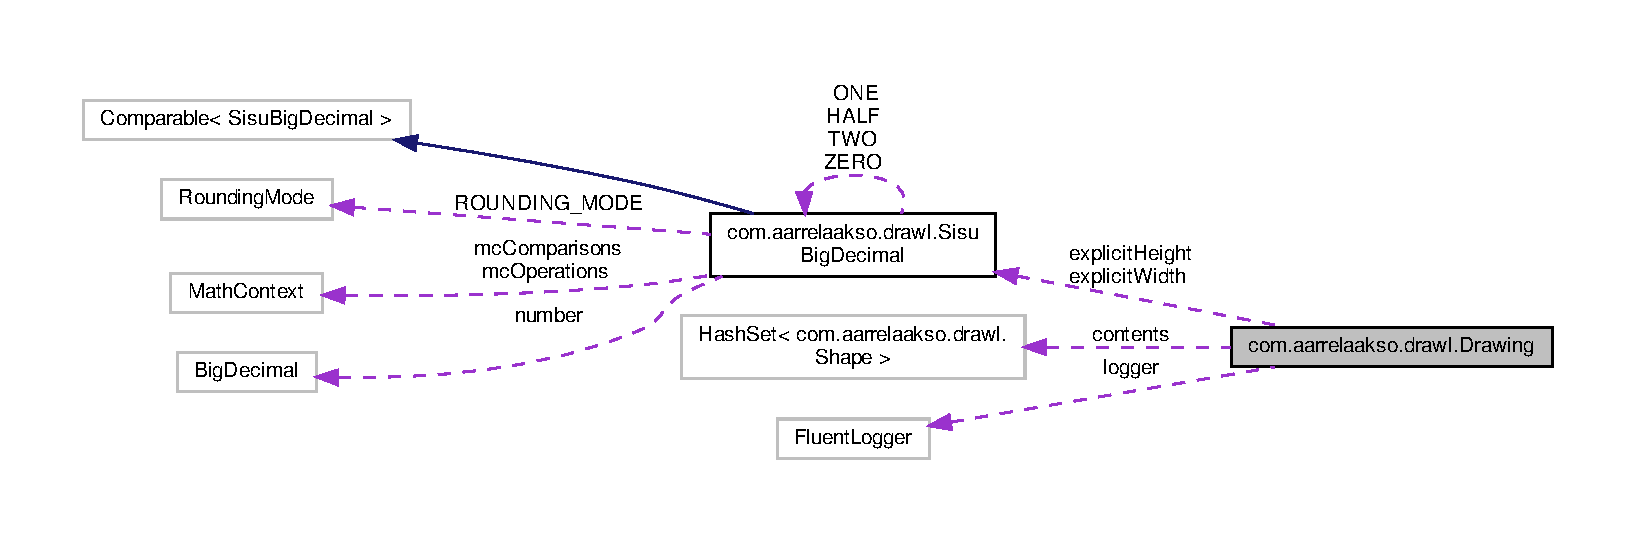
\includegraphics[width=350pt]{dd/db2/classcom_1_1aarrelaakso_1_1drawl_1_1_drawing__coll__graph}
\end{center}
\end{figure}
\subsection*{Public Member Functions}
\begin{DoxyCompactItemize}
\item 
\hyperlink{classcom_1_1aarrelaakso_1_1drawl_1_1_drawing_adc398fbdb9acaa2c09ab8f048ff45109}{Drawing} ()
\item 
final void \hyperlink{classcom_1_1aarrelaakso_1_1drawl_1_1_drawing_abb794d2aac631a7e20f3cd6948d117fe}{add} (@Not\+Null final \hyperlink{classcom_1_1aarrelaakso_1_1drawl_1_1_shape}{Shape} shape)
\begin{DoxyCompactList}\small\item\em Add a shape to this drawing. \end{DoxyCompactList}\item 
final \hyperlink{interfacecom_1_1aarrelaakso_1_1drawl_1_1_number}{Number} \hyperlink{classcom_1_1aarrelaakso_1_1drawl_1_1_drawing_ade424cd3d355473603555ad6ce746e23}{get\+Explicit\+Height} ()
\begin{DoxyCompactList}\small\item\em Get the explicit height of this \hyperlink{classcom_1_1aarrelaakso_1_1drawl_1_1_drawing}{Drawing}. \end{DoxyCompactList}\item 
final void \hyperlink{classcom_1_1aarrelaakso_1_1drawl_1_1_drawing_a4a88952ac7f26d5a3be9aa3d32e2643a}{set\+Explicit\+Height} (final Float height)
\begin{DoxyCompactList}\small\item\em Set the explicit height of this \hyperlink{classcom_1_1aarrelaakso_1_1drawl_1_1_drawing}{Drawing}. \end{DoxyCompactList}\item 
final void \hyperlink{classcom_1_1aarrelaakso_1_1drawl_1_1_drawing_a58214bce0e8aa1f15a88f6daaf0e85c6}{set\+Explicit\+Height} (final Integer height)
\begin{DoxyCompactList}\small\item\em Set the explicit height of this \hyperlink{classcom_1_1aarrelaakso_1_1drawl_1_1_drawing}{Drawing}. \end{DoxyCompactList}\item 
final \hyperlink{interfacecom_1_1aarrelaakso_1_1drawl_1_1_number}{Number} \hyperlink{classcom_1_1aarrelaakso_1_1drawl_1_1_drawing_a0de258c25c1d13e3c2d71ab6a90606ef}{get\+Explicit\+Width} ()
\begin{DoxyCompactList}\small\item\em Get the explicit width of this \hyperlink{classcom_1_1aarrelaakso_1_1drawl_1_1_drawing}{Drawing}. \end{DoxyCompactList}\item 
final void \hyperlink{classcom_1_1aarrelaakso_1_1drawl_1_1_drawing_a94179f3b7c6b4619a2b86cc9f7716a77}{set\+Explicit\+Width} (final Float width)
\begin{DoxyCompactList}\small\item\em Set the explicit width of this \hyperlink{classcom_1_1aarrelaakso_1_1drawl_1_1_drawing}{Drawing}. \end{DoxyCompactList}\item 
final void \hyperlink{classcom_1_1aarrelaakso_1_1drawl_1_1_drawing_ac3b714abeb0f6132196b8a1e50b6de41}{set\+Explicit\+Width} (final Integer width)
\begin{DoxyCompactList}\small\item\em Set the explicit width of this \hyperlink{classcom_1_1aarrelaakso_1_1drawl_1_1_drawing}{Drawing}. \end{DoxyCompactList}\item 
final \hyperlink{interfacecom_1_1aarrelaakso_1_1drawl_1_1_number}{Number} \hyperlink{classcom_1_1aarrelaakso_1_1drawl_1_1_drawing_a67991c78d1f4989b0422b6cc36d339fe}{get\+Implicit\+Width} ()
\begin{DoxyCompactList}\small\item\em Get the \hyperlink{classcom_1_1aarrelaakso_1_1drawl_1_1_s_v_g}{S\+VG} for this \hyperlink{classcom_1_1aarrelaakso_1_1drawl_1_1_drawing}{Drawing}. \end{DoxyCompactList}\item 
final String \hyperlink{classcom_1_1aarrelaakso_1_1drawl_1_1_drawing_ac005562185c059c5cd14a1df92b335d6}{get\+S\+VG} (@Not\+Null final Integer drawing\+Width, @Not\+Null final Integer drawing\+Height)
\begin{DoxyCompactList}\small\item\em Get the \hyperlink{classcom_1_1aarrelaakso_1_1drawl_1_1_s_v_g}{S\+VG} for this drawing. \end{DoxyCompactList}\item 
final String \hyperlink{classcom_1_1aarrelaakso_1_1drawl_1_1_drawing_ada7c8b8df06ba84c1334e98751730500}{get\+S\+VG} ()
\begin{DoxyCompactList}\small\item\em Get the \hyperlink{classcom_1_1aarrelaakso_1_1drawl_1_1_s_v_g}{S\+VG} for this \hyperlink{classcom_1_1aarrelaakso_1_1drawl_1_1_drawing}{Drawing}. \end{DoxyCompactList}\item 
final Integer \hyperlink{classcom_1_1aarrelaakso_1_1drawl_1_1_drawing_a3977c6a791f29d87eaad10771ed8eb80}{get\+Length} ()
\begin{DoxyCompactList}\small\item\em Gets the number of items in this \hyperlink{classcom_1_1aarrelaakso_1_1drawl_1_1_drawing}{Drawing}. \end{DoxyCompactList}\item 
final void \hyperlink{classcom_1_1aarrelaakso_1_1drawl_1_1_drawing_a4ac8a97ae89af08cf9ab01dbbe3dc010}{set\+Explicit\+Dimensions} (final Float explicit\+Width\+Of\+Drawing\+Float, final Float explicit\+Height\+Of\+Drawing\+Float)
\begin{DoxyCompactList}\small\item\em Sets the explicit dimensions of this \hyperlink{classcom_1_1aarrelaakso_1_1drawl_1_1_drawing}{Drawing}. \end{DoxyCompactList}\item 
final void \hyperlink{classcom_1_1aarrelaakso_1_1drawl_1_1_drawing_a79952c781df3b19936f0f47e2810951d}{set\+Explicit\+Dimensions} (@Not\+Null final Integer explicit\+Width\+Of\+Drawing, @Not\+Null final Integer explicit\+Height\+Of\+Drawing)
\begin{DoxyCompactList}\small\item\em Set the explicit dimensions of this \hyperlink{classcom_1_1aarrelaakso_1_1drawl_1_1_drawing}{Drawing}. \end{DoxyCompactList}\item 
final void \hyperlink{classcom_1_1aarrelaakso_1_1drawl_1_1_drawing_a3cf3359170b92a63cdcb5ab67a18562e}{write\+To\+File} (@Not\+Null final String filename, @Not\+Null final Integer width, @Not\+Null final Integer height)  throws I\+O\+Exception 
\begin{DoxyCompactList}\small\item\em Write \hyperlink{classcom_1_1aarrelaakso_1_1drawl_1_1_s_v_g}{S\+VG} representing this drawing to a file. \end{DoxyCompactList}\end{DoxyCompactItemize}
\subsection*{Protected Member Functions}
\begin{DoxyCompactItemize}
\item 
final \hyperlink{interfacecom_1_1aarrelaakso_1_1drawl_1_1_number}{Number} \hyperlink{classcom_1_1aarrelaakso_1_1drawl_1_1_drawing_a9b47750a4d38fc2db164f0a0cb0e4a42}{get\+Explicit\+To\+Implicit\+Ratio} ()
\begin{DoxyCompactList}\small\item\em Get the ratio of explicit measures to implicit measures for this \hyperlink{classcom_1_1aarrelaakso_1_1drawl_1_1_drawing}{Drawing} as a whole. \end{DoxyCompactList}\item 
final \hyperlink{interfacecom_1_1aarrelaakso_1_1drawl_1_1_number}{Number} \hyperlink{classcom_1_1aarrelaakso_1_1drawl_1_1_drawing_afd070929603e97a649a65a888b5f76da}{get\+Explicit\+Width\+Per\+Implicit\+Width} ()
\begin{DoxyCompactList}\small\item\em Get the ratio of the explicit width of this drawing to the implicit width of its contents. \end{DoxyCompactList}\end{DoxyCompactItemize}
\subsection*{Package Functions}
\begin{DoxyCompactItemize}
\item 
\hyperlink{interfacecom_1_1aarrelaakso_1_1drawl_1_1_number}{Number} \hyperlink{classcom_1_1aarrelaakso_1_1drawl_1_1_drawing_a6434cc250ea5526a5778408aef18d293}{get\+Implicit\+Width\+Of\+Contents} ()
\begin{DoxyCompactList}\small\item\em Get the implicit total width of all contents in the drawing. \end{DoxyCompactList}\end{DoxyCompactItemize}
\subsection*{Static Package Functions}
\begin{DoxyCompactItemize}
\item 
\hyperlink{classcom_1_1aarrelaakso_1_1drawl_1_1_drawing_a40ce84a6d8110f7fb23a8faad42fb05f}{\mbox{[}static initializer\mbox{]}}
\end{DoxyCompactItemize}
\subsection*{Private Member Functions}
\begin{DoxyCompactItemize}
\item 
void \hyperlink{classcom_1_1aarrelaakso_1_1drawl_1_1_drawing_a115e6b8aab01c3d54c68af9cdc67ed11}{set\+Explicit\+Height} (@Not\+Null final \hyperlink{interfacecom_1_1aarrelaakso_1_1drawl_1_1_number}{Number} drawing\+Explicit\+Height)
\begin{DoxyCompactList}\small\item\em Set the explicit height of this \hyperlink{classcom_1_1aarrelaakso_1_1drawl_1_1_drawing}{Drawing}. \end{DoxyCompactList}\item 
\hyperlink{interfacecom_1_1aarrelaakso_1_1drawl_1_1_number}{Number} \hyperlink{classcom_1_1aarrelaakso_1_1drawl_1_1_drawing_a7e165d3b122c0fd44404c20c1211c21f}{get\+Explicit\+Height\+Per\+Implicit\+Height} ()
\begin{DoxyCompactList}\small\item\em Get the ratio of the explicit height of this \hyperlink{classcom_1_1aarrelaakso_1_1drawl_1_1_drawing}{Drawing} to the implicit height of its contents. \end{DoxyCompactList}\item 
void \hyperlink{classcom_1_1aarrelaakso_1_1drawl_1_1_drawing_a547eda8e04300947a0e424f62589e5c4}{set\+Explicit\+Width} (@Not\+Null final \hyperlink{interfacecom_1_1aarrelaakso_1_1drawl_1_1_number}{Number} drawing\+Explicit\+Width)
\begin{DoxyCompactList}\small\item\em Set the explicit width of this drawing. \end{DoxyCompactList}\item 
\hyperlink{interfacecom_1_1aarrelaakso_1_1drawl_1_1_number}{Number} \hyperlink{classcom_1_1aarrelaakso_1_1drawl_1_1_drawing_a4caf5eb85285105c951522b0079f17f1}{get\+Implicit\+Height} ()
\begin{DoxyCompactList}\small\item\em Get the implicit total height of all contents in the drawing. \end{DoxyCompactList}\item 
\hyperlink{interfacecom_1_1aarrelaakso_1_1drawl_1_1_number}{Number} \hyperlink{classcom_1_1aarrelaakso_1_1drawl_1_1_drawing_a50786a75c6ca4f30ab752d276a23c1c4}{get\+Implicit\+Height\+Of\+Contents} ()
\begin{DoxyCompactList}\small\item\em Get the implicit total height of all contents in the drawing. \end{DoxyCompactList}\item 
\hyperlink{interfacecom_1_1aarrelaakso_1_1drawl_1_1_number}{Number} \hyperlink{classcom_1_1aarrelaakso_1_1drawl_1_1_drawing_a5376328fce5b40696338490ab5b65bfe}{get\+Implicit\+X\+Maximum} ()
\begin{DoxyCompactList}\small\item\em Get the maximum x-\/coordinate of this drawing in implicit terms. \end{DoxyCompactList}\item 
\hyperlink{interfacecom_1_1aarrelaakso_1_1drawl_1_1_number}{Number} \hyperlink{classcom_1_1aarrelaakso_1_1drawl_1_1_drawing_a481640a0219881863f0150b5f6439e38}{get\+Implicit\+X\+Minimum} ()
\begin{DoxyCompactList}\small\item\em Get the minimum x-\/coordinate of this drawing in implicit terms. \end{DoxyCompactList}\item 
\hyperlink{interfacecom_1_1aarrelaakso_1_1drawl_1_1_number}{Number} \hyperlink{classcom_1_1aarrelaakso_1_1drawl_1_1_drawing_a604c7e5fd692a279380aa2cd8c47a9bc}{get\+Implicit\+Y\+Maximum} ()
\begin{DoxyCompactList}\small\item\em Get the maximum y-\/coordinate of this drawing in implicit terms. \end{DoxyCompactList}\item 
\hyperlink{interfacecom_1_1aarrelaakso_1_1drawl_1_1_number}{Number} \hyperlink{classcom_1_1aarrelaakso_1_1drawl_1_1_drawing_a6bd98f6bb8616668329f07705f8f3689}{get\+Implicit\+Y\+Minimum} ()
\begin{DoxyCompactList}\small\item\em Get the minimum y-\/coordinate of this drawing in implicit terms. \end{DoxyCompactList}\item 
boolean \hyperlink{classcom_1_1aarrelaakso_1_1drawl_1_1_drawing_ab5e45e49b01dc01733156f2bd3e917ea}{is\+Explicit\+Set} ()
\begin{DoxyCompactList}\small\item\em Indicate whether the explicit dimensions of this \hyperlink{classcom_1_1aarrelaakso_1_1drawl_1_1_drawing}{Drawing} have been set. \end{DoxyCompactList}\item 
void \hyperlink{classcom_1_1aarrelaakso_1_1drawl_1_1_drawing_a54f9447ef03b883cac2bf4535e777a7a}{set\+Explicit\+Height\+Internal} (@Not\+Null final \hyperlink{interfacecom_1_1aarrelaakso_1_1drawl_1_1_number}{Number} drawing\+Explicit\+Height)
\begin{DoxyCompactList}\small\item\em Sets the explicit height of this \hyperlink{classcom_1_1aarrelaakso_1_1drawl_1_1_drawing}{Drawing}. \end{DoxyCompactList}\item 
void \hyperlink{classcom_1_1aarrelaakso_1_1drawl_1_1_drawing_a7083d7046d42a99050495007854b5908}{set\+Explicit\+Width\+Internal} (@Not\+Null final \hyperlink{interfacecom_1_1aarrelaakso_1_1drawl_1_1_number}{Number} drawing\+Explicit\+Width)
\begin{DoxyCompactList}\small\item\em Set the explicit width of this \hyperlink{classcom_1_1aarrelaakso_1_1drawl_1_1_drawing}{Drawing}. \end{DoxyCompactList}\item 
void \hyperlink{classcom_1_1aarrelaakso_1_1drawl_1_1_drawing_aa60d355859fa4dc21d2670aced9ee927}{update\+Shape} (@Not\+Null final \hyperlink{classcom_1_1aarrelaakso_1_1drawl_1_1_shape}{Shape} shape)
\begin{DoxyCompactList}\small\item\em Update the width and x-\/coordinate, height and y-\/coordinate of a single shape. \end{DoxyCompactList}\item 
void \hyperlink{classcom_1_1aarrelaakso_1_1drawl_1_1_drawing_ab55b53c2e069f28185865f5cf677c8cd}{update\+Explicit\+Height\+Of\+Shape} (@Not\+Null final \hyperlink{classcom_1_1aarrelaakso_1_1drawl_1_1_shape}{Shape} shape)
\item 
void \hyperlink{classcom_1_1aarrelaakso_1_1drawl_1_1_drawing_a5c146de66e8f3272b57322f1cee7d7d6}{update\+Explicit\+Width\+Of\+Shape} (@Not\+Null final \hyperlink{classcom_1_1aarrelaakso_1_1drawl_1_1_shape}{Shape} shape)
\item 
void \hyperlink{classcom_1_1aarrelaakso_1_1drawl_1_1_drawing_a9ae55cefe8729385c2a9cb8b9aff6763}{update\+Explicit\+X\+Position\+Of\+Shape} (@Not\+Null final \hyperlink{classcom_1_1aarrelaakso_1_1drawl_1_1_shape}{Shape} shape)
\item 
void \hyperlink{classcom_1_1aarrelaakso_1_1drawl_1_1_drawing_a52d5971daf6f95d27bcdf7650d0a9e37}{update\+Explicit\+Y\+Position\+Of\+Shape} (@Not\+Null final \hyperlink{classcom_1_1aarrelaakso_1_1drawl_1_1_shape}{Shape} shape)
\end{DoxyCompactItemize}
\subsection*{Private Attributes}
\begin{DoxyCompactItemize}
\item 
final Hash\+Set$<$ \hyperlink{classcom_1_1aarrelaakso_1_1drawl_1_1_shape}{Shape} $>$ \hyperlink{classcom_1_1aarrelaakso_1_1drawl_1_1_drawing_ab9ec6030e9f21d42852b308c482b3ccf}{contents}
\item 
\hyperlink{interfacecom_1_1aarrelaakso_1_1drawl_1_1_number}{Number} \hyperlink{classcom_1_1aarrelaakso_1_1drawl_1_1_drawing_af4ab83c7d30a2f1d1d54f247c78e3b51}{explicit\+Height}
\item 
\hyperlink{interfacecom_1_1aarrelaakso_1_1drawl_1_1_number}{Number} \hyperlink{classcom_1_1aarrelaakso_1_1drawl_1_1_drawing_a4ae6b33e0ae3b4a615e06bed22db02d7}{explicit\+Width}
\end{DoxyCompactItemize}
\subsection*{Static Private Attributes}
\begin{DoxyCompactItemize}
\item 
static final Fluent\+Logger \hyperlink{classcom_1_1aarrelaakso_1_1drawl_1_1_drawing_a9ca07608ceeb04d747e114cd1a82a3f9}{logger}
\item 
static final int \hyperlink{classcom_1_1aarrelaakso_1_1drawl_1_1_drawing_a151c12e3dc5c72fe0f1e3186de42db70}{initial\+Capacity} = 16
\item 
static final float \hyperlink{classcom_1_1aarrelaakso_1_1drawl_1_1_drawing_a853a2ba75750f3ece0036c3617ac169f}{load\+Factor} = 0.\+75f
\end{DoxyCompactItemize}


\subsection{Detailed Description}
Represents drawings. 

\subsection{Constructor \& Destructor Documentation}
\mbox{\Hypertarget{classcom_1_1aarrelaakso_1_1drawl_1_1_drawing_adc398fbdb9acaa2c09ab8f048ff45109}\label{classcom_1_1aarrelaakso_1_1drawl_1_1_drawing_adc398fbdb9acaa2c09ab8f048ff45109}} 
\index{com\+::aarrelaakso\+::drawl\+::\+Drawing@{com\+::aarrelaakso\+::drawl\+::\+Drawing}!Drawing@{Drawing}}
\index{Drawing@{Drawing}!com\+::aarrelaakso\+::drawl\+::\+Drawing@{com\+::aarrelaakso\+::drawl\+::\+Drawing}}
\subsubsection{\texorpdfstring{Drawing()}{Drawing()}}
{\footnotesize\ttfamily com.\+aarrelaakso.\+drawl.\+Drawing.\+Drawing (\begin{DoxyParamCaption}{ }\end{DoxyParamCaption})}



\subsection{Member Function Documentation}
\mbox{\Hypertarget{classcom_1_1aarrelaakso_1_1drawl_1_1_drawing_a40ce84a6d8110f7fb23a8faad42fb05f}\label{classcom_1_1aarrelaakso_1_1drawl_1_1_drawing_a40ce84a6d8110f7fb23a8faad42fb05f}} 
\index{com\+::aarrelaakso\+::drawl\+::\+Drawing@{com\+::aarrelaakso\+::drawl\+::\+Drawing}!\mbox{[}static initializer\mbox{]}@{[static initializer]}}
\index{\mbox{[}static initializer\mbox{]}@{[static initializer]}!com\+::aarrelaakso\+::drawl\+::\+Drawing@{com\+::aarrelaakso\+::drawl\+::\+Drawing}}
\subsubsection{\texorpdfstring{[static initializer]()}{[static initializer]()}}
{\footnotesize\ttfamily com.\+aarrelaakso.\+drawl.\+Drawing.\mbox{[}static initializer\mbox{]} (\begin{DoxyParamCaption}{ }\end{DoxyParamCaption})\hspace{0.3cm}{\ttfamily [static]}, {\ttfamily [package]}}

\mbox{\Hypertarget{classcom_1_1aarrelaakso_1_1drawl_1_1_drawing_abb794d2aac631a7e20f3cd6948d117fe}\label{classcom_1_1aarrelaakso_1_1drawl_1_1_drawing_abb794d2aac631a7e20f3cd6948d117fe}} 
\index{com\+::aarrelaakso\+::drawl\+::\+Drawing@{com\+::aarrelaakso\+::drawl\+::\+Drawing}!add@{add}}
\index{add@{add}!com\+::aarrelaakso\+::drawl\+::\+Drawing@{com\+::aarrelaakso\+::drawl\+::\+Drawing}}
\subsubsection{\texorpdfstring{add()}{add()}}
{\footnotesize\ttfamily final void com.\+aarrelaakso.\+drawl.\+Drawing.\+add (\begin{DoxyParamCaption}\item[{@Not\+Null final \hyperlink{classcom_1_1aarrelaakso_1_1drawl_1_1_shape}{Shape}}]{shape }\end{DoxyParamCaption})}



Add a shape to this drawing. 


\begin{DoxyParams}{Parameters}
{\em shape} & The shape to add \\
\hline
\end{DoxyParams}
\mbox{\Hypertarget{classcom_1_1aarrelaakso_1_1drawl_1_1_drawing_ade424cd3d355473603555ad6ce746e23}\label{classcom_1_1aarrelaakso_1_1drawl_1_1_drawing_ade424cd3d355473603555ad6ce746e23}} 
\index{com\+::aarrelaakso\+::drawl\+::\+Drawing@{com\+::aarrelaakso\+::drawl\+::\+Drawing}!get\+Explicit\+Height@{get\+Explicit\+Height}}
\index{get\+Explicit\+Height@{get\+Explicit\+Height}!com\+::aarrelaakso\+::drawl\+::\+Drawing@{com\+::aarrelaakso\+::drawl\+::\+Drawing}}
\subsubsection{\texorpdfstring{get\+Explicit\+Height()}{getExplicitHeight()}}
{\footnotesize\ttfamily final \hyperlink{interfacecom_1_1aarrelaakso_1_1drawl_1_1_number}{Number} com.\+aarrelaakso.\+drawl.\+Drawing.\+get\+Explicit\+Height (\begin{DoxyParamCaption}{ }\end{DoxyParamCaption})}



Get the explicit height of this \hyperlink{classcom_1_1aarrelaakso_1_1drawl_1_1_drawing}{Drawing}. 

\begin{DoxyReturn}{Returns}
The explicit height of this \hyperlink{classcom_1_1aarrelaakso_1_1drawl_1_1_drawing}{Drawing}, or null if the drawing has length zero or the explicit dimensions have not been set. 
\end{DoxyReturn}
\mbox{\Hypertarget{classcom_1_1aarrelaakso_1_1drawl_1_1_drawing_a7e165d3b122c0fd44404c20c1211c21f}\label{classcom_1_1aarrelaakso_1_1drawl_1_1_drawing_a7e165d3b122c0fd44404c20c1211c21f}} 
\index{com\+::aarrelaakso\+::drawl\+::\+Drawing@{com\+::aarrelaakso\+::drawl\+::\+Drawing}!get\+Explicit\+Height\+Per\+Implicit\+Height@{get\+Explicit\+Height\+Per\+Implicit\+Height}}
\index{get\+Explicit\+Height\+Per\+Implicit\+Height@{get\+Explicit\+Height\+Per\+Implicit\+Height}!com\+::aarrelaakso\+::drawl\+::\+Drawing@{com\+::aarrelaakso\+::drawl\+::\+Drawing}}
\subsubsection{\texorpdfstring{get\+Explicit\+Height\+Per\+Implicit\+Height()}{getExplicitHeightPerImplicitHeight()}}
{\footnotesize\ttfamily \hyperlink{interfacecom_1_1aarrelaakso_1_1drawl_1_1_number}{Number} com.\+aarrelaakso.\+drawl.\+Drawing.\+get\+Explicit\+Height\+Per\+Implicit\+Height (\begin{DoxyParamCaption}{ }\end{DoxyParamCaption})\hspace{0.3cm}{\ttfamily [private]}}



Get the ratio of the explicit height of this \hyperlink{classcom_1_1aarrelaakso_1_1drawl_1_1_drawing}{Drawing} to the implicit height of its contents. 

\begin{DoxyReturn}{Returns}
The ratio of the explicit height of this \hyperlink{classcom_1_1aarrelaakso_1_1drawl_1_1_drawing}{Drawing} to the implicit height of its contents 
\end{DoxyReturn}
\mbox{\Hypertarget{classcom_1_1aarrelaakso_1_1drawl_1_1_drawing_a9b47750a4d38fc2db164f0a0cb0e4a42}\label{classcom_1_1aarrelaakso_1_1drawl_1_1_drawing_a9b47750a4d38fc2db164f0a0cb0e4a42}} 
\index{com\+::aarrelaakso\+::drawl\+::\+Drawing@{com\+::aarrelaakso\+::drawl\+::\+Drawing}!get\+Explicit\+To\+Implicit\+Ratio@{get\+Explicit\+To\+Implicit\+Ratio}}
\index{get\+Explicit\+To\+Implicit\+Ratio@{get\+Explicit\+To\+Implicit\+Ratio}!com\+::aarrelaakso\+::drawl\+::\+Drawing@{com\+::aarrelaakso\+::drawl\+::\+Drawing}}
\subsubsection{\texorpdfstring{get\+Explicit\+To\+Implicit\+Ratio()}{getExplicitToImplicitRatio()}}
{\footnotesize\ttfamily final \hyperlink{interfacecom_1_1aarrelaakso_1_1drawl_1_1_number}{Number} com.\+aarrelaakso.\+drawl.\+Drawing.\+get\+Explicit\+To\+Implicit\+Ratio (\begin{DoxyParamCaption}{ }\end{DoxyParamCaption})\hspace{0.3cm}{\ttfamily [protected]}}



Get the ratio of explicit measures to implicit measures for this \hyperlink{classcom_1_1aarrelaakso_1_1drawl_1_1_drawing}{Drawing} as a whole. 

This is the ratio of the explicit dimension of the \hyperlink{classcom_1_1aarrelaakso_1_1drawl_1_1_drawing}{Drawing} to the implicit dimension of its contents. 

This method is different from \hyperlink{classcom_1_1aarrelaakso_1_1drawl_1_1_drawing_a7e165d3b122c0fd44404c20c1211c21f}{get\+Explicit\+Height\+Per\+Implicit\+Height()} and \hyperlink{classcom_1_1aarrelaakso_1_1drawl_1_1_drawing_afd070929603e97a649a65a888b5f76da}{get\+Explicit\+Width\+Per\+Implicit\+Width()} in that it takes into account both height constraints and width constraints.

\begin{DoxyReturn}{Returns}
The ratio of explicit measures to implicit measures for this diagram as a whole. 
\end{DoxyReturn}
\mbox{\Hypertarget{classcom_1_1aarrelaakso_1_1drawl_1_1_drawing_a0de258c25c1d13e3c2d71ab6a90606ef}\label{classcom_1_1aarrelaakso_1_1drawl_1_1_drawing_a0de258c25c1d13e3c2d71ab6a90606ef}} 
\index{com\+::aarrelaakso\+::drawl\+::\+Drawing@{com\+::aarrelaakso\+::drawl\+::\+Drawing}!get\+Explicit\+Width@{get\+Explicit\+Width}}
\index{get\+Explicit\+Width@{get\+Explicit\+Width}!com\+::aarrelaakso\+::drawl\+::\+Drawing@{com\+::aarrelaakso\+::drawl\+::\+Drawing}}
\subsubsection{\texorpdfstring{get\+Explicit\+Width()}{getExplicitWidth()}}
{\footnotesize\ttfamily final \hyperlink{interfacecom_1_1aarrelaakso_1_1drawl_1_1_number}{Number} com.\+aarrelaakso.\+drawl.\+Drawing.\+get\+Explicit\+Width (\begin{DoxyParamCaption}{ }\end{DoxyParamCaption})}



Get the explicit width of this \hyperlink{classcom_1_1aarrelaakso_1_1drawl_1_1_drawing}{Drawing}. 

\begin{DoxyReturn}{Returns}
The explicit width of this \hyperlink{classcom_1_1aarrelaakso_1_1drawl_1_1_drawing}{Drawing}, or null if the drawing has length zero or the explicit dimensions have not been set. 
\end{DoxyReturn}
\mbox{\Hypertarget{classcom_1_1aarrelaakso_1_1drawl_1_1_drawing_afd070929603e97a649a65a888b5f76da}\label{classcom_1_1aarrelaakso_1_1drawl_1_1_drawing_afd070929603e97a649a65a888b5f76da}} 
\index{com\+::aarrelaakso\+::drawl\+::\+Drawing@{com\+::aarrelaakso\+::drawl\+::\+Drawing}!get\+Explicit\+Width\+Per\+Implicit\+Width@{get\+Explicit\+Width\+Per\+Implicit\+Width}}
\index{get\+Explicit\+Width\+Per\+Implicit\+Width@{get\+Explicit\+Width\+Per\+Implicit\+Width}!com\+::aarrelaakso\+::drawl\+::\+Drawing@{com\+::aarrelaakso\+::drawl\+::\+Drawing}}
\subsubsection{\texorpdfstring{get\+Explicit\+Width\+Per\+Implicit\+Width()}{getExplicitWidthPerImplicitWidth()}}
{\footnotesize\ttfamily final \hyperlink{interfacecom_1_1aarrelaakso_1_1drawl_1_1_number}{Number} com.\+aarrelaakso.\+drawl.\+Drawing.\+get\+Explicit\+Width\+Per\+Implicit\+Width (\begin{DoxyParamCaption}{ }\end{DoxyParamCaption})\hspace{0.3cm}{\ttfamily [protected]}}



Get the ratio of the explicit width of this drawing to the implicit width of its contents. 

\begin{DoxyReturn}{Returns}
The ratio of the explicit width of this drawing to the implicit width of its contents. 
\end{DoxyReturn}
\mbox{\Hypertarget{classcom_1_1aarrelaakso_1_1drawl_1_1_drawing_a4caf5eb85285105c951522b0079f17f1}\label{classcom_1_1aarrelaakso_1_1drawl_1_1_drawing_a4caf5eb85285105c951522b0079f17f1}} 
\index{com\+::aarrelaakso\+::drawl\+::\+Drawing@{com\+::aarrelaakso\+::drawl\+::\+Drawing}!get\+Implicit\+Height@{get\+Implicit\+Height}}
\index{get\+Implicit\+Height@{get\+Implicit\+Height}!com\+::aarrelaakso\+::drawl\+::\+Drawing@{com\+::aarrelaakso\+::drawl\+::\+Drawing}}
\subsubsection{\texorpdfstring{get\+Implicit\+Height()}{getImplicitHeight()}}
{\footnotesize\ttfamily \hyperlink{interfacecom_1_1aarrelaakso_1_1drawl_1_1_number}{Number} com.\+aarrelaakso.\+drawl.\+Drawing.\+get\+Implicit\+Height (\begin{DoxyParamCaption}{ }\end{DoxyParamCaption})\hspace{0.3cm}{\ttfamily [private]}}



Get the implicit total height of all contents in the drawing. 

Provides public access to the implicit height of the contents. \mbox{\Hypertarget{classcom_1_1aarrelaakso_1_1drawl_1_1_drawing_a50786a75c6ca4f30ab752d276a23c1c4}\label{classcom_1_1aarrelaakso_1_1drawl_1_1_drawing_a50786a75c6ca4f30ab752d276a23c1c4}} 
\index{com\+::aarrelaakso\+::drawl\+::\+Drawing@{com\+::aarrelaakso\+::drawl\+::\+Drawing}!get\+Implicit\+Height\+Of\+Contents@{get\+Implicit\+Height\+Of\+Contents}}
\index{get\+Implicit\+Height\+Of\+Contents@{get\+Implicit\+Height\+Of\+Contents}!com\+::aarrelaakso\+::drawl\+::\+Drawing@{com\+::aarrelaakso\+::drawl\+::\+Drawing}}
\subsubsection{\texorpdfstring{get\+Implicit\+Height\+Of\+Contents()}{getImplicitHeightOfContents()}}
{\footnotesize\ttfamily \hyperlink{interfacecom_1_1aarrelaakso_1_1drawl_1_1_number}{Number} com.\+aarrelaakso.\+drawl.\+Drawing.\+get\+Implicit\+Height\+Of\+Contents (\begin{DoxyParamCaption}{ }\end{DoxyParamCaption})\hspace{0.3cm}{\ttfamily [private]}}



Get the implicit total height of all contents in the drawing. 

\begin{DoxyReturn}{Returns}
the implicit total height of all contents in this drawing 
\end{DoxyReturn}
\mbox{\Hypertarget{classcom_1_1aarrelaakso_1_1drawl_1_1_drawing_a67991c78d1f4989b0422b6cc36d339fe}\label{classcom_1_1aarrelaakso_1_1drawl_1_1_drawing_a67991c78d1f4989b0422b6cc36d339fe}} 
\index{com\+::aarrelaakso\+::drawl\+::\+Drawing@{com\+::aarrelaakso\+::drawl\+::\+Drawing}!get\+Implicit\+Width@{get\+Implicit\+Width}}
\index{get\+Implicit\+Width@{get\+Implicit\+Width}!com\+::aarrelaakso\+::drawl\+::\+Drawing@{com\+::aarrelaakso\+::drawl\+::\+Drawing}}
\subsubsection{\texorpdfstring{get\+Implicit\+Width()}{getImplicitWidth()}}
{\footnotesize\ttfamily final \hyperlink{interfacecom_1_1aarrelaakso_1_1drawl_1_1_number}{Number} com.\+aarrelaakso.\+drawl.\+Drawing.\+get\+Implicit\+Width (\begin{DoxyParamCaption}{ }\end{DoxyParamCaption})}



Get the \hyperlink{classcom_1_1aarrelaakso_1_1drawl_1_1_s_v_g}{S\+VG} for this \hyperlink{classcom_1_1aarrelaakso_1_1drawl_1_1_drawing}{Drawing}. 


\begin{DoxyParams}{Parameters}
{\em drawing\+Width} & The desired width of the output; the type is Float to match the \hyperlink{classcom_1_1aarrelaakso_1_1drawl_1_1_s_v_g}{S\+VG} spec for numeric precision. \\
\hline
{\em drawing\+Height} & The desired height of the output; the type is Float to match the \hyperlink{classcom_1_1aarrelaakso_1_1drawl_1_1_s_v_g}{S\+VG} spec for numeric precision. \\
\hline
\end{DoxyParams}
\begin{DoxyReturn}{Returns}
A string of valid \hyperlink{classcom_1_1aarrelaakso_1_1drawl_1_1_s_v_g}{S\+VG} that depicts the drawing within the bounds of drawing\+Width and drawing\+Height. Get the implicit total width of all contents in this \hyperlink{classcom_1_1aarrelaakso_1_1drawl_1_1_drawing}{Drawing}. 
\end{DoxyReturn}
Provides public access to the implicit width of the contents for testing. \mbox{\Hypertarget{classcom_1_1aarrelaakso_1_1drawl_1_1_drawing_a6434cc250ea5526a5778408aef18d293}\label{classcom_1_1aarrelaakso_1_1drawl_1_1_drawing_a6434cc250ea5526a5778408aef18d293}} 
\index{com\+::aarrelaakso\+::drawl\+::\+Drawing@{com\+::aarrelaakso\+::drawl\+::\+Drawing}!get\+Implicit\+Width\+Of\+Contents@{get\+Implicit\+Width\+Of\+Contents}}
\index{get\+Implicit\+Width\+Of\+Contents@{get\+Implicit\+Width\+Of\+Contents}!com\+::aarrelaakso\+::drawl\+::\+Drawing@{com\+::aarrelaakso\+::drawl\+::\+Drawing}}
\subsubsection{\texorpdfstring{get\+Implicit\+Width\+Of\+Contents()}{getImplicitWidthOfContents()}}
{\footnotesize\ttfamily \hyperlink{interfacecom_1_1aarrelaakso_1_1drawl_1_1_number}{Number} com.\+aarrelaakso.\+drawl.\+Drawing.\+get\+Implicit\+Width\+Of\+Contents (\begin{DoxyParamCaption}{ }\end{DoxyParamCaption})\hspace{0.3cm}{\ttfamily [package]}}



Get the implicit total width of all contents in the drawing. 

\begin{DoxyReturn}{Returns}
the implicit total width of all contents in this drawing 
\end{DoxyReturn}
\mbox{\Hypertarget{classcom_1_1aarrelaakso_1_1drawl_1_1_drawing_a5376328fce5b40696338490ab5b65bfe}\label{classcom_1_1aarrelaakso_1_1drawl_1_1_drawing_a5376328fce5b40696338490ab5b65bfe}} 
\index{com\+::aarrelaakso\+::drawl\+::\+Drawing@{com\+::aarrelaakso\+::drawl\+::\+Drawing}!get\+Implicit\+X\+Maximum@{get\+Implicit\+X\+Maximum}}
\index{get\+Implicit\+X\+Maximum@{get\+Implicit\+X\+Maximum}!com\+::aarrelaakso\+::drawl\+::\+Drawing@{com\+::aarrelaakso\+::drawl\+::\+Drawing}}
\subsubsection{\texorpdfstring{get\+Implicit\+X\+Maximum()}{getImplicitXMaximum()}}
{\footnotesize\ttfamily \hyperlink{interfacecom_1_1aarrelaakso_1_1drawl_1_1_number}{Number} com.\+aarrelaakso.\+drawl.\+Drawing.\+get\+Implicit\+X\+Maximum (\begin{DoxyParamCaption}{ }\end{DoxyParamCaption})\hspace{0.3cm}{\ttfamily [private]}}



Get the maximum x-\/coordinate of this drawing in implicit terms. 

The maximum x-\/coordinate is the right edge of the drawing. \mbox{\Hypertarget{classcom_1_1aarrelaakso_1_1drawl_1_1_drawing_a481640a0219881863f0150b5f6439e38}\label{classcom_1_1aarrelaakso_1_1drawl_1_1_drawing_a481640a0219881863f0150b5f6439e38}} 
\index{com\+::aarrelaakso\+::drawl\+::\+Drawing@{com\+::aarrelaakso\+::drawl\+::\+Drawing}!get\+Implicit\+X\+Minimum@{get\+Implicit\+X\+Minimum}}
\index{get\+Implicit\+X\+Minimum@{get\+Implicit\+X\+Minimum}!com\+::aarrelaakso\+::drawl\+::\+Drawing@{com\+::aarrelaakso\+::drawl\+::\+Drawing}}
\subsubsection{\texorpdfstring{get\+Implicit\+X\+Minimum()}{getImplicitXMinimum()}}
{\footnotesize\ttfamily \hyperlink{interfacecom_1_1aarrelaakso_1_1drawl_1_1_number}{Number} com.\+aarrelaakso.\+drawl.\+Drawing.\+get\+Implicit\+X\+Minimum (\begin{DoxyParamCaption}{ }\end{DoxyParamCaption})\hspace{0.3cm}{\ttfamily [private]}}



Get the minimum x-\/coordinate of this drawing in implicit terms. 

The minimum x-\/coordinate is the leftmost edge of the drawing. \mbox{\Hypertarget{classcom_1_1aarrelaakso_1_1drawl_1_1_drawing_a604c7e5fd692a279380aa2cd8c47a9bc}\label{classcom_1_1aarrelaakso_1_1drawl_1_1_drawing_a604c7e5fd692a279380aa2cd8c47a9bc}} 
\index{com\+::aarrelaakso\+::drawl\+::\+Drawing@{com\+::aarrelaakso\+::drawl\+::\+Drawing}!get\+Implicit\+Y\+Maximum@{get\+Implicit\+Y\+Maximum}}
\index{get\+Implicit\+Y\+Maximum@{get\+Implicit\+Y\+Maximum}!com\+::aarrelaakso\+::drawl\+::\+Drawing@{com\+::aarrelaakso\+::drawl\+::\+Drawing}}
\subsubsection{\texorpdfstring{get\+Implicit\+Y\+Maximum()}{getImplicitYMaximum()}}
{\footnotesize\ttfamily \hyperlink{interfacecom_1_1aarrelaakso_1_1drawl_1_1_number}{Number} com.\+aarrelaakso.\+drawl.\+Drawing.\+get\+Implicit\+Y\+Maximum (\begin{DoxyParamCaption}{ }\end{DoxyParamCaption})\hspace{0.3cm}{\ttfamily [private]}}



Get the maximum y-\/coordinate of this drawing in implicit terms. 

The maximum y-\/coordinate is the top edge of the drawing. \mbox{\Hypertarget{classcom_1_1aarrelaakso_1_1drawl_1_1_drawing_a6bd98f6bb8616668329f07705f8f3689}\label{classcom_1_1aarrelaakso_1_1drawl_1_1_drawing_a6bd98f6bb8616668329f07705f8f3689}} 
\index{com\+::aarrelaakso\+::drawl\+::\+Drawing@{com\+::aarrelaakso\+::drawl\+::\+Drawing}!get\+Implicit\+Y\+Minimum@{get\+Implicit\+Y\+Minimum}}
\index{get\+Implicit\+Y\+Minimum@{get\+Implicit\+Y\+Minimum}!com\+::aarrelaakso\+::drawl\+::\+Drawing@{com\+::aarrelaakso\+::drawl\+::\+Drawing}}
\subsubsection{\texorpdfstring{get\+Implicit\+Y\+Minimum()}{getImplicitYMinimum()}}
{\footnotesize\ttfamily \hyperlink{interfacecom_1_1aarrelaakso_1_1drawl_1_1_number}{Number} com.\+aarrelaakso.\+drawl.\+Drawing.\+get\+Implicit\+Y\+Minimum (\begin{DoxyParamCaption}{ }\end{DoxyParamCaption})\hspace{0.3cm}{\ttfamily [private]}}



Get the minimum y-\/coordinate of this drawing in implicit terms. 

The minimum y-\/coordinate is the bottom edge of the drawing. \mbox{\Hypertarget{classcom_1_1aarrelaakso_1_1drawl_1_1_drawing_a3977c6a791f29d87eaad10771ed8eb80}\label{classcom_1_1aarrelaakso_1_1drawl_1_1_drawing_a3977c6a791f29d87eaad10771ed8eb80}} 
\index{com\+::aarrelaakso\+::drawl\+::\+Drawing@{com\+::aarrelaakso\+::drawl\+::\+Drawing}!get\+Length@{get\+Length}}
\index{get\+Length@{get\+Length}!com\+::aarrelaakso\+::drawl\+::\+Drawing@{com\+::aarrelaakso\+::drawl\+::\+Drawing}}
\subsubsection{\texorpdfstring{get\+Length()}{getLength()}}
{\footnotesize\ttfamily final Integer com.\+aarrelaakso.\+drawl.\+Drawing.\+get\+Length (\begin{DoxyParamCaption}{ }\end{DoxyParamCaption})}



Gets the number of items in this \hyperlink{classcom_1_1aarrelaakso_1_1drawl_1_1_drawing}{Drawing}. 

\begin{DoxyReturn}{Returns}
the number of items in this \hyperlink{classcom_1_1aarrelaakso_1_1drawl_1_1_drawing}{Drawing} 
\end{DoxyReturn}
\mbox{\Hypertarget{classcom_1_1aarrelaakso_1_1drawl_1_1_drawing_ac005562185c059c5cd14a1df92b335d6}\label{classcom_1_1aarrelaakso_1_1drawl_1_1_drawing_ac005562185c059c5cd14a1df92b335d6}} 
\index{com\+::aarrelaakso\+::drawl\+::\+Drawing@{com\+::aarrelaakso\+::drawl\+::\+Drawing}!get\+S\+VG@{get\+S\+VG}}
\index{get\+S\+VG@{get\+S\+VG}!com\+::aarrelaakso\+::drawl\+::\+Drawing@{com\+::aarrelaakso\+::drawl\+::\+Drawing}}
\subsubsection{\texorpdfstring{get\+S\+V\+G()}{getSVG()}\hspace{0.1cm}{\footnotesize\ttfamily [1/2]}}
{\footnotesize\ttfamily final String com.\+aarrelaakso.\+drawl.\+Drawing.\+get\+S\+VG (\begin{DoxyParamCaption}\item[{@Not\+Null final Integer}]{drawing\+Width,  }\item[{@Not\+Null final Integer}]{drawing\+Height }\end{DoxyParamCaption})}



Get the \hyperlink{classcom_1_1aarrelaakso_1_1drawl_1_1_s_v_g}{S\+VG} for this drawing. 


\begin{DoxyParams}{Parameters}
{\em drawing\+Width} & The desired width of the output; the type is Integer to allow for common use cases. \\
\hline
{\em drawing\+Height} & The desired height of the output; the type is Integer to allow for common use cases. \\
\hline
\end{DoxyParams}
\begin{DoxyReturn}{Returns}
A string of valid \hyperlink{classcom_1_1aarrelaakso_1_1drawl_1_1_s_v_g}{S\+VG} that depicts the drawing within the bounds of drawing\+Width and drawing\+Height. 
\end{DoxyReturn}
\mbox{\Hypertarget{classcom_1_1aarrelaakso_1_1drawl_1_1_drawing_ada7c8b8df06ba84c1334e98751730500}\label{classcom_1_1aarrelaakso_1_1drawl_1_1_drawing_ada7c8b8df06ba84c1334e98751730500}} 
\index{com\+::aarrelaakso\+::drawl\+::\+Drawing@{com\+::aarrelaakso\+::drawl\+::\+Drawing}!get\+S\+VG@{get\+S\+VG}}
\index{get\+S\+VG@{get\+S\+VG}!com\+::aarrelaakso\+::drawl\+::\+Drawing@{com\+::aarrelaakso\+::drawl\+::\+Drawing}}
\subsubsection{\texorpdfstring{get\+S\+V\+G()}{getSVG()}\hspace{0.1cm}{\footnotesize\ttfamily [2/2]}}
{\footnotesize\ttfamily final String com.\+aarrelaakso.\+drawl.\+Drawing.\+get\+S\+VG (\begin{DoxyParamCaption}{ }\end{DoxyParamCaption})}



Get the \hyperlink{classcom_1_1aarrelaakso_1_1drawl_1_1_s_v_g}{S\+VG} for this \hyperlink{classcom_1_1aarrelaakso_1_1drawl_1_1_drawing}{Drawing}. 

Assumes that the explicit width and height have been set

\begin{DoxyReturn}{Returns}
A string of valid \hyperlink{classcom_1_1aarrelaakso_1_1drawl_1_1_s_v_g}{S\+VG} that depicts the drawing within the bounds of the explicit width and height 
\end{DoxyReturn}
\mbox{\Hypertarget{classcom_1_1aarrelaakso_1_1drawl_1_1_drawing_ab5e45e49b01dc01733156f2bd3e917ea}\label{classcom_1_1aarrelaakso_1_1drawl_1_1_drawing_ab5e45e49b01dc01733156f2bd3e917ea}} 
\index{com\+::aarrelaakso\+::drawl\+::\+Drawing@{com\+::aarrelaakso\+::drawl\+::\+Drawing}!is\+Explicit\+Set@{is\+Explicit\+Set}}
\index{is\+Explicit\+Set@{is\+Explicit\+Set}!com\+::aarrelaakso\+::drawl\+::\+Drawing@{com\+::aarrelaakso\+::drawl\+::\+Drawing}}
\subsubsection{\texorpdfstring{is\+Explicit\+Set()}{isExplicitSet()}}
{\footnotesize\ttfamily boolean com.\+aarrelaakso.\+drawl.\+Drawing.\+is\+Explicit\+Set (\begin{DoxyParamCaption}{ }\end{DoxyParamCaption})\hspace{0.3cm}{\ttfamily [private]}}



Indicate whether the explicit dimensions of this \hyperlink{classcom_1_1aarrelaakso_1_1drawl_1_1_drawing}{Drawing} have been set. 

\begin{DoxyReturn}{Returns}
{\ttfamily T\+R\+UE} if the explicit dimensions of this \hyperlink{classcom_1_1aarrelaakso_1_1drawl_1_1_drawing}{Drawing} have been set, {\ttfamily F\+A\+L\+SE} otherwise. 
\end{DoxyReturn}
\mbox{\Hypertarget{classcom_1_1aarrelaakso_1_1drawl_1_1_drawing_a4ac8a97ae89af08cf9ab01dbbe3dc010}\label{classcom_1_1aarrelaakso_1_1drawl_1_1_drawing_a4ac8a97ae89af08cf9ab01dbbe3dc010}} 
\index{com\+::aarrelaakso\+::drawl\+::\+Drawing@{com\+::aarrelaakso\+::drawl\+::\+Drawing}!set\+Explicit\+Dimensions@{set\+Explicit\+Dimensions}}
\index{set\+Explicit\+Dimensions@{set\+Explicit\+Dimensions}!com\+::aarrelaakso\+::drawl\+::\+Drawing@{com\+::aarrelaakso\+::drawl\+::\+Drawing}}
\subsubsection{\texorpdfstring{set\+Explicit\+Dimensions()}{setExplicitDimensions()}\hspace{0.1cm}{\footnotesize\ttfamily [1/2]}}
{\footnotesize\ttfamily final void com.\+aarrelaakso.\+drawl.\+Drawing.\+set\+Explicit\+Dimensions (\begin{DoxyParamCaption}\item[{final Float}]{explicit\+Width\+Of\+Drawing\+Float,  }\item[{final Float}]{explicit\+Height\+Of\+Drawing\+Float }\end{DoxyParamCaption})}



Sets the explicit dimensions of this \hyperlink{classcom_1_1aarrelaakso_1_1drawl_1_1_drawing}{Drawing}. 

It is preferable to do it this way rather than setting width and height separately.


\begin{DoxyParams}{Parameters}
{\em explicit\+Width\+Of\+Drawing\+Float} & The explicit width of the \hyperlink{classcom_1_1aarrelaakso_1_1drawl_1_1_drawing}{Drawing}. \\
\hline
{\em explicit\+Height\+Of\+Drawing\+Float} & The explicit height of the \hyperlink{classcom_1_1aarrelaakso_1_1drawl_1_1_drawing}{Drawing}. \\
\hline
\end{DoxyParams}
\mbox{\Hypertarget{classcom_1_1aarrelaakso_1_1drawl_1_1_drawing_a79952c781df3b19936f0f47e2810951d}\label{classcom_1_1aarrelaakso_1_1drawl_1_1_drawing_a79952c781df3b19936f0f47e2810951d}} 
\index{com\+::aarrelaakso\+::drawl\+::\+Drawing@{com\+::aarrelaakso\+::drawl\+::\+Drawing}!set\+Explicit\+Dimensions@{set\+Explicit\+Dimensions}}
\index{set\+Explicit\+Dimensions@{set\+Explicit\+Dimensions}!com\+::aarrelaakso\+::drawl\+::\+Drawing@{com\+::aarrelaakso\+::drawl\+::\+Drawing}}
\subsubsection{\texorpdfstring{set\+Explicit\+Dimensions()}{setExplicitDimensions()}\hspace{0.1cm}{\footnotesize\ttfamily [2/2]}}
{\footnotesize\ttfamily final void com.\+aarrelaakso.\+drawl.\+Drawing.\+set\+Explicit\+Dimensions (\begin{DoxyParamCaption}\item[{@Not\+Null final Integer}]{explicit\+Width\+Of\+Drawing,  }\item[{@Not\+Null final Integer}]{explicit\+Height\+Of\+Drawing }\end{DoxyParamCaption})}



Set the explicit dimensions of this \hyperlink{classcom_1_1aarrelaakso_1_1drawl_1_1_drawing}{Drawing}. 

It is preferable to do it this way rather than setting the dimensions separately. 

This convenience method takes Integer parameters to allow for common use cases.


\begin{DoxyParams}{Parameters}
{\em explicit\+Width\+Of\+Drawing} & The explicit width of the \hyperlink{classcom_1_1aarrelaakso_1_1drawl_1_1_drawing}{Drawing}. \\
\hline
{\em explicit\+Height\+Of\+Drawing} & The explicit height of the \hyperlink{classcom_1_1aarrelaakso_1_1drawl_1_1_drawing}{Drawing}. \\
\hline
\end{DoxyParams}
\mbox{\Hypertarget{classcom_1_1aarrelaakso_1_1drawl_1_1_drawing_a115e6b8aab01c3d54c68af9cdc67ed11}\label{classcom_1_1aarrelaakso_1_1drawl_1_1_drawing_a115e6b8aab01c3d54c68af9cdc67ed11}} 
\index{com\+::aarrelaakso\+::drawl\+::\+Drawing@{com\+::aarrelaakso\+::drawl\+::\+Drawing}!set\+Explicit\+Height@{set\+Explicit\+Height}}
\index{set\+Explicit\+Height@{set\+Explicit\+Height}!com\+::aarrelaakso\+::drawl\+::\+Drawing@{com\+::aarrelaakso\+::drawl\+::\+Drawing}}
\subsubsection{\texorpdfstring{set\+Explicit\+Height()}{setExplicitHeight()}\hspace{0.1cm}{\footnotesize\ttfamily [1/3]}}
{\footnotesize\ttfamily void com.\+aarrelaakso.\+drawl.\+Drawing.\+set\+Explicit\+Height (\begin{DoxyParamCaption}\item[{@Not\+Null final \hyperlink{interfacecom_1_1aarrelaakso_1_1drawl_1_1_number}{Number}}]{drawing\+Explicit\+Height }\end{DoxyParamCaption})\hspace{0.3cm}{\ttfamily [private]}}



Set the explicit height of this \hyperlink{classcom_1_1aarrelaakso_1_1drawl_1_1_drawing}{Drawing}. 

This method also calculates the explicit heights and y positions of all the drawing\textquotesingle{}s contents. If the explicit width of this \hyperlink{classcom_1_1aarrelaakso_1_1drawl_1_1_drawing}{Drawing} is not known, then this method also sets the explicit width to match the aspect ratio of the contents.


\begin{DoxyParams}{Parameters}
{\em drawing\+Explicit\+Height} & The explicit height of the drawing. \\
\hline
\end{DoxyParams}
\mbox{\Hypertarget{classcom_1_1aarrelaakso_1_1drawl_1_1_drawing_a4a88952ac7f26d5a3be9aa3d32e2643a}\label{classcom_1_1aarrelaakso_1_1drawl_1_1_drawing_a4a88952ac7f26d5a3be9aa3d32e2643a}} 
\index{com\+::aarrelaakso\+::drawl\+::\+Drawing@{com\+::aarrelaakso\+::drawl\+::\+Drawing}!set\+Explicit\+Height@{set\+Explicit\+Height}}
\index{set\+Explicit\+Height@{set\+Explicit\+Height}!com\+::aarrelaakso\+::drawl\+::\+Drawing@{com\+::aarrelaakso\+::drawl\+::\+Drawing}}
\subsubsection{\texorpdfstring{set\+Explicit\+Height()}{setExplicitHeight()}\hspace{0.1cm}{\footnotesize\ttfamily [2/3]}}
{\footnotesize\ttfamily final void com.\+aarrelaakso.\+drawl.\+Drawing.\+set\+Explicit\+Height (\begin{DoxyParamCaption}\item[{final Float}]{height }\end{DoxyParamCaption})}



Set the explicit height of this \hyperlink{classcom_1_1aarrelaakso_1_1drawl_1_1_drawing}{Drawing}. 


\begin{DoxyParams}{Parameters}
{\em height} & the explicit height of the \hyperlink{classcom_1_1aarrelaakso_1_1drawl_1_1_drawing}{Drawing}; it is a Float to match the precision allowed by the \hyperlink{classcom_1_1aarrelaakso_1_1drawl_1_1_s_v_g}{S\+VG} spec. \\
\hline
\end{DoxyParams}
\mbox{\Hypertarget{classcom_1_1aarrelaakso_1_1drawl_1_1_drawing_a58214bce0e8aa1f15a88f6daaf0e85c6}\label{classcom_1_1aarrelaakso_1_1drawl_1_1_drawing_a58214bce0e8aa1f15a88f6daaf0e85c6}} 
\index{com\+::aarrelaakso\+::drawl\+::\+Drawing@{com\+::aarrelaakso\+::drawl\+::\+Drawing}!set\+Explicit\+Height@{set\+Explicit\+Height}}
\index{set\+Explicit\+Height@{set\+Explicit\+Height}!com\+::aarrelaakso\+::drawl\+::\+Drawing@{com\+::aarrelaakso\+::drawl\+::\+Drawing}}
\subsubsection{\texorpdfstring{set\+Explicit\+Height()}{setExplicitHeight()}\hspace{0.1cm}{\footnotesize\ttfamily [3/3]}}
{\footnotesize\ttfamily final void com.\+aarrelaakso.\+drawl.\+Drawing.\+set\+Explicit\+Height (\begin{DoxyParamCaption}\item[{final Integer}]{height }\end{DoxyParamCaption})}



Set the explicit height of this \hyperlink{classcom_1_1aarrelaakso_1_1drawl_1_1_drawing}{Drawing}. 


\begin{DoxyParams}{Parameters}
{\em height} & The explicit height of the \hyperlink{classcom_1_1aarrelaakso_1_1drawl_1_1_drawing}{Drawing}; it is an Integer to allow for common use cases. \\
\hline
\end{DoxyParams}
\mbox{\Hypertarget{classcom_1_1aarrelaakso_1_1drawl_1_1_drawing_a54f9447ef03b883cac2bf4535e777a7a}\label{classcom_1_1aarrelaakso_1_1drawl_1_1_drawing_a54f9447ef03b883cac2bf4535e777a7a}} 
\index{com\+::aarrelaakso\+::drawl\+::\+Drawing@{com\+::aarrelaakso\+::drawl\+::\+Drawing}!set\+Explicit\+Height\+Internal@{set\+Explicit\+Height\+Internal}}
\index{set\+Explicit\+Height\+Internal@{set\+Explicit\+Height\+Internal}!com\+::aarrelaakso\+::drawl\+::\+Drawing@{com\+::aarrelaakso\+::drawl\+::\+Drawing}}
\subsubsection{\texorpdfstring{set\+Explicit\+Height\+Internal()}{setExplicitHeightInternal()}}
{\footnotesize\ttfamily void com.\+aarrelaakso.\+drawl.\+Drawing.\+set\+Explicit\+Height\+Internal (\begin{DoxyParamCaption}\item[{@Not\+Null final \hyperlink{interfacecom_1_1aarrelaakso_1_1drawl_1_1_number}{Number}}]{drawing\+Explicit\+Height }\end{DoxyParamCaption})\hspace{0.3cm}{\ttfamily [private]}}



Sets the explicit height of this \hyperlink{classcom_1_1aarrelaakso_1_1drawl_1_1_drawing}{Drawing}. 

Use this to allow logging changes to internal height.


\begin{DoxyParams}{Parameters}
{\em drawing\+Explicit\+Height} & the new explicit height of the \hyperlink{classcom_1_1aarrelaakso_1_1drawl_1_1_drawing}{Drawing}. \\
\hline
\end{DoxyParams}
\mbox{\Hypertarget{classcom_1_1aarrelaakso_1_1drawl_1_1_drawing_a547eda8e04300947a0e424f62589e5c4}\label{classcom_1_1aarrelaakso_1_1drawl_1_1_drawing_a547eda8e04300947a0e424f62589e5c4}} 
\index{com\+::aarrelaakso\+::drawl\+::\+Drawing@{com\+::aarrelaakso\+::drawl\+::\+Drawing}!set\+Explicit\+Width@{set\+Explicit\+Width}}
\index{set\+Explicit\+Width@{set\+Explicit\+Width}!com\+::aarrelaakso\+::drawl\+::\+Drawing@{com\+::aarrelaakso\+::drawl\+::\+Drawing}}
\subsubsection{\texorpdfstring{set\+Explicit\+Width()}{setExplicitWidth()}\hspace{0.1cm}{\footnotesize\ttfamily [1/3]}}
{\footnotesize\ttfamily void com.\+aarrelaakso.\+drawl.\+Drawing.\+set\+Explicit\+Width (\begin{DoxyParamCaption}\item[{@Not\+Null final \hyperlink{interfacecom_1_1aarrelaakso_1_1drawl_1_1_number}{Number}}]{drawing\+Explicit\+Width }\end{DoxyParamCaption})\hspace{0.3cm}{\ttfamily [private]}}



Set the explicit width of this drawing. 

This method also calculates the explicit widths and x positions of all the drawing\textquotesingle{}s contents.


\begin{DoxyParams}{Parameters}
{\em drawing\+Explicit\+Width} & The explicit width of the drawing. \\
\hline
\end{DoxyParams}
\mbox{\Hypertarget{classcom_1_1aarrelaakso_1_1drawl_1_1_drawing_a94179f3b7c6b4619a2b86cc9f7716a77}\label{classcom_1_1aarrelaakso_1_1drawl_1_1_drawing_a94179f3b7c6b4619a2b86cc9f7716a77}} 
\index{com\+::aarrelaakso\+::drawl\+::\+Drawing@{com\+::aarrelaakso\+::drawl\+::\+Drawing}!set\+Explicit\+Width@{set\+Explicit\+Width}}
\index{set\+Explicit\+Width@{set\+Explicit\+Width}!com\+::aarrelaakso\+::drawl\+::\+Drawing@{com\+::aarrelaakso\+::drawl\+::\+Drawing}}
\subsubsection{\texorpdfstring{set\+Explicit\+Width()}{setExplicitWidth()}\hspace{0.1cm}{\footnotesize\ttfamily [2/3]}}
{\footnotesize\ttfamily final void com.\+aarrelaakso.\+drawl.\+Drawing.\+set\+Explicit\+Width (\begin{DoxyParamCaption}\item[{final Float}]{width }\end{DoxyParamCaption})}



Set the explicit width of this \hyperlink{classcom_1_1aarrelaakso_1_1drawl_1_1_drawing}{Drawing}. 


\begin{DoxyParams}{Parameters}
{\em width} & the explicit width of the \hyperlink{classcom_1_1aarrelaakso_1_1drawl_1_1_drawing}{Drawing}; it is a Float to match the precision allowed by the \hyperlink{classcom_1_1aarrelaakso_1_1drawl_1_1_s_v_g}{S\+VG} spec. \\
\hline
\end{DoxyParams}
\mbox{\Hypertarget{classcom_1_1aarrelaakso_1_1drawl_1_1_drawing_ac3b714abeb0f6132196b8a1e50b6de41}\label{classcom_1_1aarrelaakso_1_1drawl_1_1_drawing_ac3b714abeb0f6132196b8a1e50b6de41}} 
\index{com\+::aarrelaakso\+::drawl\+::\+Drawing@{com\+::aarrelaakso\+::drawl\+::\+Drawing}!set\+Explicit\+Width@{set\+Explicit\+Width}}
\index{set\+Explicit\+Width@{set\+Explicit\+Width}!com\+::aarrelaakso\+::drawl\+::\+Drawing@{com\+::aarrelaakso\+::drawl\+::\+Drawing}}
\subsubsection{\texorpdfstring{set\+Explicit\+Width()}{setExplicitWidth()}\hspace{0.1cm}{\footnotesize\ttfamily [3/3]}}
{\footnotesize\ttfamily final void com.\+aarrelaakso.\+drawl.\+Drawing.\+set\+Explicit\+Width (\begin{DoxyParamCaption}\item[{final Integer}]{width }\end{DoxyParamCaption})}



Set the explicit width of this \hyperlink{classcom_1_1aarrelaakso_1_1drawl_1_1_drawing}{Drawing}. 


\begin{DoxyParams}{Parameters}
{\em width} & The explicit width of the \hyperlink{classcom_1_1aarrelaakso_1_1drawl_1_1_drawing}{Drawing}; it is an Integer to allow for common use cases. \\
\hline
\end{DoxyParams}
\mbox{\Hypertarget{classcom_1_1aarrelaakso_1_1drawl_1_1_drawing_a7083d7046d42a99050495007854b5908}\label{classcom_1_1aarrelaakso_1_1drawl_1_1_drawing_a7083d7046d42a99050495007854b5908}} 
\index{com\+::aarrelaakso\+::drawl\+::\+Drawing@{com\+::aarrelaakso\+::drawl\+::\+Drawing}!set\+Explicit\+Width\+Internal@{set\+Explicit\+Width\+Internal}}
\index{set\+Explicit\+Width\+Internal@{set\+Explicit\+Width\+Internal}!com\+::aarrelaakso\+::drawl\+::\+Drawing@{com\+::aarrelaakso\+::drawl\+::\+Drawing}}
\subsubsection{\texorpdfstring{set\+Explicit\+Width\+Internal()}{setExplicitWidthInternal()}}
{\footnotesize\ttfamily void com.\+aarrelaakso.\+drawl.\+Drawing.\+set\+Explicit\+Width\+Internal (\begin{DoxyParamCaption}\item[{@Not\+Null final \hyperlink{interfacecom_1_1aarrelaakso_1_1drawl_1_1_number}{Number}}]{drawing\+Explicit\+Width }\end{DoxyParamCaption})\hspace{0.3cm}{\ttfamily [private]}}



Set the explicit width of this \hyperlink{classcom_1_1aarrelaakso_1_1drawl_1_1_drawing}{Drawing}. 

Use this to allow logging changes to internal height.


\begin{DoxyParams}{Parameters}
{\em drawing\+Explicit\+Width} & the new explicit width of the \hyperlink{classcom_1_1aarrelaakso_1_1drawl_1_1_drawing}{Drawing}. \\
\hline
\end{DoxyParams}
\mbox{\Hypertarget{classcom_1_1aarrelaakso_1_1drawl_1_1_drawing_ab55b53c2e069f28185865f5cf677c8cd}\label{classcom_1_1aarrelaakso_1_1drawl_1_1_drawing_ab55b53c2e069f28185865f5cf677c8cd}} 
\index{com\+::aarrelaakso\+::drawl\+::\+Drawing@{com\+::aarrelaakso\+::drawl\+::\+Drawing}!update\+Explicit\+Height\+Of\+Shape@{update\+Explicit\+Height\+Of\+Shape}}
\index{update\+Explicit\+Height\+Of\+Shape@{update\+Explicit\+Height\+Of\+Shape}!com\+::aarrelaakso\+::drawl\+::\+Drawing@{com\+::aarrelaakso\+::drawl\+::\+Drawing}}
\subsubsection{\texorpdfstring{update\+Explicit\+Height\+Of\+Shape()}{updateExplicitHeightOfShape()}}
{\footnotesize\ttfamily void com.\+aarrelaakso.\+drawl.\+Drawing.\+update\+Explicit\+Height\+Of\+Shape (\begin{DoxyParamCaption}\item[{@Not\+Null final \hyperlink{classcom_1_1aarrelaakso_1_1drawl_1_1_shape}{Shape}}]{shape }\end{DoxyParamCaption})\hspace{0.3cm}{\ttfamily [private]}}

\mbox{\Hypertarget{classcom_1_1aarrelaakso_1_1drawl_1_1_drawing_a5c146de66e8f3272b57322f1cee7d7d6}\label{classcom_1_1aarrelaakso_1_1drawl_1_1_drawing_a5c146de66e8f3272b57322f1cee7d7d6}} 
\index{com\+::aarrelaakso\+::drawl\+::\+Drawing@{com\+::aarrelaakso\+::drawl\+::\+Drawing}!update\+Explicit\+Width\+Of\+Shape@{update\+Explicit\+Width\+Of\+Shape}}
\index{update\+Explicit\+Width\+Of\+Shape@{update\+Explicit\+Width\+Of\+Shape}!com\+::aarrelaakso\+::drawl\+::\+Drawing@{com\+::aarrelaakso\+::drawl\+::\+Drawing}}
\subsubsection{\texorpdfstring{update\+Explicit\+Width\+Of\+Shape()}{updateExplicitWidthOfShape()}}
{\footnotesize\ttfamily void com.\+aarrelaakso.\+drawl.\+Drawing.\+update\+Explicit\+Width\+Of\+Shape (\begin{DoxyParamCaption}\item[{@Not\+Null final \hyperlink{classcom_1_1aarrelaakso_1_1drawl_1_1_shape}{Shape}}]{shape }\end{DoxyParamCaption})\hspace{0.3cm}{\ttfamily [private]}}

\mbox{\Hypertarget{classcom_1_1aarrelaakso_1_1drawl_1_1_drawing_a9ae55cefe8729385c2a9cb8b9aff6763}\label{classcom_1_1aarrelaakso_1_1drawl_1_1_drawing_a9ae55cefe8729385c2a9cb8b9aff6763}} 
\index{com\+::aarrelaakso\+::drawl\+::\+Drawing@{com\+::aarrelaakso\+::drawl\+::\+Drawing}!update\+Explicit\+X\+Position\+Of\+Shape@{update\+Explicit\+X\+Position\+Of\+Shape}}
\index{update\+Explicit\+X\+Position\+Of\+Shape@{update\+Explicit\+X\+Position\+Of\+Shape}!com\+::aarrelaakso\+::drawl\+::\+Drawing@{com\+::aarrelaakso\+::drawl\+::\+Drawing}}
\subsubsection{\texorpdfstring{update\+Explicit\+X\+Position\+Of\+Shape()}{updateExplicitXPositionOfShape()}}
{\footnotesize\ttfamily void com.\+aarrelaakso.\+drawl.\+Drawing.\+update\+Explicit\+X\+Position\+Of\+Shape (\begin{DoxyParamCaption}\item[{@Not\+Null final \hyperlink{classcom_1_1aarrelaakso_1_1drawl_1_1_shape}{Shape}}]{shape }\end{DoxyParamCaption})\hspace{0.3cm}{\ttfamily [private]}}

\mbox{\Hypertarget{classcom_1_1aarrelaakso_1_1drawl_1_1_drawing_a52d5971daf6f95d27bcdf7650d0a9e37}\label{classcom_1_1aarrelaakso_1_1drawl_1_1_drawing_a52d5971daf6f95d27bcdf7650d0a9e37}} 
\index{com\+::aarrelaakso\+::drawl\+::\+Drawing@{com\+::aarrelaakso\+::drawl\+::\+Drawing}!update\+Explicit\+Y\+Position\+Of\+Shape@{update\+Explicit\+Y\+Position\+Of\+Shape}}
\index{update\+Explicit\+Y\+Position\+Of\+Shape@{update\+Explicit\+Y\+Position\+Of\+Shape}!com\+::aarrelaakso\+::drawl\+::\+Drawing@{com\+::aarrelaakso\+::drawl\+::\+Drawing}}
\subsubsection{\texorpdfstring{update\+Explicit\+Y\+Position\+Of\+Shape()}{updateExplicitYPositionOfShape()}}
{\footnotesize\ttfamily void com.\+aarrelaakso.\+drawl.\+Drawing.\+update\+Explicit\+Y\+Position\+Of\+Shape (\begin{DoxyParamCaption}\item[{@Not\+Null final \hyperlink{classcom_1_1aarrelaakso_1_1drawl_1_1_shape}{Shape}}]{shape }\end{DoxyParamCaption})\hspace{0.3cm}{\ttfamily [private]}}

\mbox{\Hypertarget{classcom_1_1aarrelaakso_1_1drawl_1_1_drawing_aa60d355859fa4dc21d2670aced9ee927}\label{classcom_1_1aarrelaakso_1_1drawl_1_1_drawing_aa60d355859fa4dc21d2670aced9ee927}} 
\index{com\+::aarrelaakso\+::drawl\+::\+Drawing@{com\+::aarrelaakso\+::drawl\+::\+Drawing}!update\+Shape@{update\+Shape}}
\index{update\+Shape@{update\+Shape}!com\+::aarrelaakso\+::drawl\+::\+Drawing@{com\+::aarrelaakso\+::drawl\+::\+Drawing}}
\subsubsection{\texorpdfstring{update\+Shape()}{updateShape()}}
{\footnotesize\ttfamily void com.\+aarrelaakso.\+drawl.\+Drawing.\+update\+Shape (\begin{DoxyParamCaption}\item[{@Not\+Null final \hyperlink{classcom_1_1aarrelaakso_1_1drawl_1_1_shape}{Shape}}]{shape }\end{DoxyParamCaption})\hspace{0.3cm}{\ttfamily [private]}}



Update the width and x-\/coordinate, height and y-\/coordinate of a single shape. 

Called by \hyperlink{classcom_1_1aarrelaakso_1_1drawl_1_1_drawing_a547eda8e04300947a0e424f62589e5c4}{set\+Explicit\+Width()} \mbox{\Hypertarget{classcom_1_1aarrelaakso_1_1drawl_1_1_drawing_a3cf3359170b92a63cdcb5ab67a18562e}\label{classcom_1_1aarrelaakso_1_1drawl_1_1_drawing_a3cf3359170b92a63cdcb5ab67a18562e}} 
\index{com\+::aarrelaakso\+::drawl\+::\+Drawing@{com\+::aarrelaakso\+::drawl\+::\+Drawing}!write\+To\+File@{write\+To\+File}}
\index{write\+To\+File@{write\+To\+File}!com\+::aarrelaakso\+::drawl\+::\+Drawing@{com\+::aarrelaakso\+::drawl\+::\+Drawing}}
\subsubsection{\texorpdfstring{write\+To\+File()}{writeToFile()}}
{\footnotesize\ttfamily final void com.\+aarrelaakso.\+drawl.\+Drawing.\+write\+To\+File (\begin{DoxyParamCaption}\item[{@Not\+Null final String}]{filename,  }\item[{@Not\+Null final Integer}]{width,  }\item[{@Not\+Null final Integer}]{height }\end{DoxyParamCaption}) throws I\+O\+Exception}



Write \hyperlink{classcom_1_1aarrelaakso_1_1drawl_1_1_s_v_g}{S\+VG} representing this drawing to a file. 


\begin{DoxyParams}{Parameters}
{\em filename} & The name of the file to which to write. \\
\hline
\end{DoxyParams}

\begin{DoxyExceptions}{Exceptions}
{\em I\+O\+Exception} & If there is a problem writing to the file. \\
\hline
\end{DoxyExceptions}


\subsection{Member Data Documentation}
\mbox{\Hypertarget{classcom_1_1aarrelaakso_1_1drawl_1_1_drawing_ab9ec6030e9f21d42852b308c482b3ccf}\label{classcom_1_1aarrelaakso_1_1drawl_1_1_drawing_ab9ec6030e9f21d42852b308c482b3ccf}} 
\index{com\+::aarrelaakso\+::drawl\+::\+Drawing@{com\+::aarrelaakso\+::drawl\+::\+Drawing}!contents@{contents}}
\index{contents@{contents}!com\+::aarrelaakso\+::drawl\+::\+Drawing@{com\+::aarrelaakso\+::drawl\+::\+Drawing}}
\subsubsection{\texorpdfstring{contents}{contents}}
{\footnotesize\ttfamily final Hash\+Set$<$\hyperlink{classcom_1_1aarrelaakso_1_1drawl_1_1_shape}{Shape}$>$ com.\+aarrelaakso.\+drawl.\+Drawing.\+contents\hspace{0.3cm}{\ttfamily [private]}}

\mbox{\Hypertarget{classcom_1_1aarrelaakso_1_1drawl_1_1_drawing_af4ab83c7d30a2f1d1d54f247c78e3b51}\label{classcom_1_1aarrelaakso_1_1drawl_1_1_drawing_af4ab83c7d30a2f1d1d54f247c78e3b51}} 
\index{com\+::aarrelaakso\+::drawl\+::\+Drawing@{com\+::aarrelaakso\+::drawl\+::\+Drawing}!explicit\+Height@{explicit\+Height}}
\index{explicit\+Height@{explicit\+Height}!com\+::aarrelaakso\+::drawl\+::\+Drawing@{com\+::aarrelaakso\+::drawl\+::\+Drawing}}
\subsubsection{\texorpdfstring{explicit\+Height}{explicitHeight}}
{\footnotesize\ttfamily \hyperlink{interfacecom_1_1aarrelaakso_1_1drawl_1_1_number}{Number} com.\+aarrelaakso.\+drawl.\+Drawing.\+explicit\+Height\hspace{0.3cm}{\ttfamily [private]}}

\mbox{\Hypertarget{classcom_1_1aarrelaakso_1_1drawl_1_1_drawing_a4ae6b33e0ae3b4a615e06bed22db02d7}\label{classcom_1_1aarrelaakso_1_1drawl_1_1_drawing_a4ae6b33e0ae3b4a615e06bed22db02d7}} 
\index{com\+::aarrelaakso\+::drawl\+::\+Drawing@{com\+::aarrelaakso\+::drawl\+::\+Drawing}!explicit\+Width@{explicit\+Width}}
\index{explicit\+Width@{explicit\+Width}!com\+::aarrelaakso\+::drawl\+::\+Drawing@{com\+::aarrelaakso\+::drawl\+::\+Drawing}}
\subsubsection{\texorpdfstring{explicit\+Width}{explicitWidth}}
{\footnotesize\ttfamily \hyperlink{interfacecom_1_1aarrelaakso_1_1drawl_1_1_number}{Number} com.\+aarrelaakso.\+drawl.\+Drawing.\+explicit\+Width\hspace{0.3cm}{\ttfamily [private]}}

\mbox{\Hypertarget{classcom_1_1aarrelaakso_1_1drawl_1_1_drawing_a151c12e3dc5c72fe0f1e3186de42db70}\label{classcom_1_1aarrelaakso_1_1drawl_1_1_drawing_a151c12e3dc5c72fe0f1e3186de42db70}} 
\index{com\+::aarrelaakso\+::drawl\+::\+Drawing@{com\+::aarrelaakso\+::drawl\+::\+Drawing}!initial\+Capacity@{initial\+Capacity}}
\index{initial\+Capacity@{initial\+Capacity}!com\+::aarrelaakso\+::drawl\+::\+Drawing@{com\+::aarrelaakso\+::drawl\+::\+Drawing}}
\subsubsection{\texorpdfstring{initial\+Capacity}{initialCapacity}}
{\footnotesize\ttfamily final int com.\+aarrelaakso.\+drawl.\+Drawing.\+initial\+Capacity = 16\hspace{0.3cm}{\ttfamily [static]}, {\ttfamily [private]}}

\mbox{\Hypertarget{classcom_1_1aarrelaakso_1_1drawl_1_1_drawing_a853a2ba75750f3ece0036c3617ac169f}\label{classcom_1_1aarrelaakso_1_1drawl_1_1_drawing_a853a2ba75750f3ece0036c3617ac169f}} 
\index{com\+::aarrelaakso\+::drawl\+::\+Drawing@{com\+::aarrelaakso\+::drawl\+::\+Drawing}!load\+Factor@{load\+Factor}}
\index{load\+Factor@{load\+Factor}!com\+::aarrelaakso\+::drawl\+::\+Drawing@{com\+::aarrelaakso\+::drawl\+::\+Drawing}}
\subsubsection{\texorpdfstring{load\+Factor}{loadFactor}}
{\footnotesize\ttfamily final float com.\+aarrelaakso.\+drawl.\+Drawing.\+load\+Factor = 0.\+75f\hspace{0.3cm}{\ttfamily [static]}, {\ttfamily [private]}}

\mbox{\Hypertarget{classcom_1_1aarrelaakso_1_1drawl_1_1_drawing_a9ca07608ceeb04d747e114cd1a82a3f9}\label{classcom_1_1aarrelaakso_1_1drawl_1_1_drawing_a9ca07608ceeb04d747e114cd1a82a3f9}} 
\index{com\+::aarrelaakso\+::drawl\+::\+Drawing@{com\+::aarrelaakso\+::drawl\+::\+Drawing}!logger@{logger}}
\index{logger@{logger}!com\+::aarrelaakso\+::drawl\+::\+Drawing@{com\+::aarrelaakso\+::drawl\+::\+Drawing}}
\subsubsection{\texorpdfstring{logger}{logger}}
{\footnotesize\ttfamily final Fluent\+Logger com.\+aarrelaakso.\+drawl.\+Drawing.\+logger\hspace{0.3cm}{\ttfamily [static]}, {\ttfamily [private]}}



The documentation for this class was generated from the following file\+:\begin{DoxyCompactItemize}
\item 
/mnt/d/\+One\+Drive/\+Documents/src/drawl/src/main/java/com/aarrelaakso/drawl/\hyperlink{_drawing_8java}{Drawing.\+java}\end{DoxyCompactItemize}

\hypertarget{classcom_1_1aarrelaakso_1_1drawl_1_1_drawl_number}{}\section{com.\+aarrelaakso.\+drawl.\+Drawl\+Number Class Reference}
\label{classcom_1_1aarrelaakso_1_1drawl_1_1_drawl_number}\index{com.\+aarrelaakso.\+drawl.\+Drawl\+Number@{com.\+aarrelaakso.\+drawl.\+Drawl\+Number}}


Class for mathematical operations with Double values that have a similar A\+PI to that of the Big\+Decimal class.  


\subsection*{Public Member Functions}
\begin{DoxyCompactItemize}
\item 
boolean \hyperlink{classcom_1_1aarrelaakso_1_1drawl_1_1_drawl_number_aae7f631882c9400f8fcc7d5c04441d2b}{is\+Integer\+Value} (@Not\+Null final Big\+Decimal bd)
\begin{DoxyCompactList}\small\item\em Test whether a Big\+Decimal is a mathematical integer. \end{DoxyCompactList}\item 
boolean \hyperlink{classcom_1_1aarrelaakso_1_1drawl_1_1_drawl_number_a6400df8bf99b502371a39347f8d7dff2}{is\+Integer\+Value} (final float val)
\begin{DoxyCompactList}\small\item\em Test whether a float is a mathematical integer. \end{DoxyCompactList}\item 
\hyperlink{interfacecom_1_1aarrelaakso_1_1drawl_1_1_number}{Number} \hyperlink{classcom_1_1aarrelaakso_1_1drawl_1_1_drawl_number_a2bdcf6f7da129ae45c46f7e91bc65636}{abs} ()
\begin{DoxyCompactList}\small\item\em Returns absolute value of this number. \end{DoxyCompactList}\item 
\hyperlink{interfacecom_1_1aarrelaakso_1_1drawl_1_1_number}{Number} \hyperlink{classcom_1_1aarrelaakso_1_1drawl_1_1_drawl_number_a484120b1cacb13f1266bf1d3f002ce3d}{add} (@Not\+Null final \hyperlink{interfacecom_1_1aarrelaakso_1_1drawl_1_1_number}{Number} augend)
\begin{DoxyCompactList}\small\item\em Performs addition operation. \end{DoxyCompactList}\item 
\hyperlink{interfacecom_1_1aarrelaakso_1_1drawl_1_1_number}{Number} \hyperlink{classcom_1_1aarrelaakso_1_1drawl_1_1_drawl_number_adf7216ecb118a2bbd1d4aba6a51110bc}{add} (final double x)
\begin{DoxyCompactList}\small\item\em Performs addition operation. \end{DoxyCompactList}\item 
\hyperlink{interfacecom_1_1aarrelaakso_1_1drawl_1_1_number}{Number} \hyperlink{classcom_1_1aarrelaakso_1_1drawl_1_1_drawl_number_a1ecd88ae492b29cf92013f7441f488f8}{add} (@Not\+Null final \hyperlink{interfacecom_1_1aarrelaakso_1_1drawl_1_1_number}{Number} augend, final Math\+Context mc)
\begin{DoxyCompactList}\small\item\em Returns a \hyperlink{classcom_1_1aarrelaakso_1_1drawl_1_1_drawl_number}{Drawl\+Number} whose value is (this + augend), with rounding according to the context settings. \end{DoxyCompactList}\item 
Big\+Decimal \hyperlink{classcom_1_1aarrelaakso_1_1drawl_1_1_drawl_number_acf97abc572acd173a4d8cd6c5b5c2ecd}{big\+Decimal\+Value} ()
\begin{DoxyCompactList}\small\item\em Converts this Sisu\+Big\+Decimal to a Big\+Decimal. \end{DoxyCompactList}\item 
int \hyperlink{classcom_1_1aarrelaakso_1_1drawl_1_1_drawl_number_a40d2c6535f85306aaf5b6e5886c51266}{compare\+To} (@Not\+Null final \hyperlink{interfacecom_1_1aarrelaakso_1_1drawl_1_1_number}{Number} comparator)
\begin{DoxyCompactList}\small\item\em Compares this \hyperlink{classcom_1_1aarrelaakso_1_1drawl_1_1_drawl_number}{Drawl\+Number} with the specified \hyperlink{interfacecom_1_1aarrelaakso_1_1drawl_1_1_number}{Number}. \end{DoxyCompactList}\item 
int \hyperlink{classcom_1_1aarrelaakso_1_1drawl_1_1_drawl_number_ab2624aa98592bb5dd20990c7f5921024}{compare\+To\+Fuzzy} (@Not\+Null final \hyperlink{interfacecom_1_1aarrelaakso_1_1drawl_1_1_number}{Number} comparator)
\begin{DoxyCompactList}\small\item\em Compare this \hyperlink{classcom_1_1aarrelaakso_1_1drawl_1_1_drawl_number}{Drawl\+Number} to another using the default Math\+Context. \end{DoxyCompactList}\item 
int \hyperlink{classcom_1_1aarrelaakso_1_1drawl_1_1_drawl_number_a67bb221c313ba22d920db646d130d66f}{compare\+To\+Fuzzy} (@Not\+Null final \hyperlink{interfacecom_1_1aarrelaakso_1_1drawl_1_1_number}{Number} comparator, final Math\+Context mc)
\begin{DoxyCompactList}\small\item\em Compares this \hyperlink{classcom_1_1aarrelaakso_1_1drawl_1_1_drawl_number}{Drawl\+Number} to another \hyperlink{interfacecom_1_1aarrelaakso_1_1drawl_1_1_number}{Number} fuzzily. \end{DoxyCompactList}\item 
\hyperlink{classcom_1_1aarrelaakso_1_1drawl_1_1_drawl_number_remainder_pair}{Drawl\+Number\+Remainder\+Pair} \hyperlink{classcom_1_1aarrelaakso_1_1drawl_1_1_drawl_number_a452c8b23180fe298592093adde0fa87e}{div\+With\+Remainder} (@Not\+Null final \hyperlink{interfacecom_1_1aarrelaakso_1_1drawl_1_1_number}{Number} divisor, final int precision)
\begin{DoxyCompactList}\small\item\em Performs division operation and returns the result with remainder. \end{DoxyCompactList}\item 
\hyperlink{classcom_1_1aarrelaakso_1_1drawl_1_1_drawl_number_remainder_pair}{Drawl\+Number\+Remainder\+Pair} \hyperlink{classcom_1_1aarrelaakso_1_1drawl_1_1_drawl_number_a6dc7cefb2574b9675ab3bc099760cbd2}{div\+With\+Remainder} (final double x, final int precision)
\begin{DoxyCompactList}\small\item\em Performs division operation and returns the result with remainder. \end{DoxyCompactList}\item 
\hyperlink{interfacecom_1_1aarrelaakso_1_1drawl_1_1_number}{Number} \hyperlink{classcom_1_1aarrelaakso_1_1drawl_1_1_drawl_number_ad6350a9965757a1ffeb859d71ee0219e}{divide} (@Not\+Null final \hyperlink{interfacecom_1_1aarrelaakso_1_1drawl_1_1_number}{Number} divisor, final Math\+Context math\+Context)
\begin{DoxyCompactList}\small\item\em Divides with \hyperlink{classcom_1_1aarrelaakso_1_1drawl_1_1_drawl_number}{Drawl\+Number} by another. \end{DoxyCompactList}\item 
final \hyperlink{interfacecom_1_1aarrelaakso_1_1drawl_1_1_number}{Number} \hyperlink{classcom_1_1aarrelaakso_1_1drawl_1_1_drawl_number_a24ee9901f4d84a2fc086d4e727bf40c7}{divide} (@Not\+Null final \hyperlink{interfacecom_1_1aarrelaakso_1_1drawl_1_1_number}{Number} divisor, final int precision)
\begin{DoxyCompactList}\small\item\em Divides this \hyperlink{classcom_1_1aarrelaakso_1_1drawl_1_1_drawl_number}{Drawl\+Number} by another \hyperlink{interfacecom_1_1aarrelaakso_1_1drawl_1_1_number}{Number}. \end{DoxyCompactList}\item 
\hyperlink{interfacecom_1_1aarrelaakso_1_1drawl_1_1_number}{Number} \hyperlink{classcom_1_1aarrelaakso_1_1drawl_1_1_drawl_number_a4ba0f1728e95fe494d440c04228041f7}{divide} (final double x, final int precision)
\begin{DoxyCompactList}\small\item\em Divides this \hyperlink{classcom_1_1aarrelaakso_1_1drawl_1_1_drawl_number}{Drawl\+Number} by a Double. \end{DoxyCompactList}\item 
double \hyperlink{classcom_1_1aarrelaakso_1_1drawl_1_1_drawl_number_af5e6d77e51e7b6167d18acec2eb26877}{double\+Value} ()
\begin{DoxyCompactList}\small\item\em Returns double representation of this number. \end{DoxyCompactList}\item 
boolean \hyperlink{classcom_1_1aarrelaakso_1_1drawl_1_1_drawl_number_ad5b1c1aea2f1d2d04a9064a3041059c5}{equals} (@Not\+Null final \hyperlink{interfacecom_1_1aarrelaakso_1_1drawl_1_1_number}{Number} x)
\begin{DoxyCompactList}\small\item\em Returns whether this number is equal with the other number. \end{DoxyCompactList}\item 
boolean \hyperlink{classcom_1_1aarrelaakso_1_1drawl_1_1_drawl_number_a09dfa96894d84cc9734e41bf4a88ae3b}{equals} (final double x)
\begin{DoxyCompactList}\small\item\em Returns whether this number is equal with the other number. \end{DoxyCompactList}\item 
boolean \hyperlink{classcom_1_1aarrelaakso_1_1drawl_1_1_drawl_number_a54d65831347b02b14569ddfc021a4ade}{equals} (final Object obj)
\begin{DoxyCompactList}\small\item\em Compares this Sisu\+Big\+Decimal with the specified Object for equality. \end{DoxyCompactList}\item 
Float \hyperlink{classcom_1_1aarrelaakso_1_1drawl_1_1_drawl_number_ae8442cbd5cc7ab0c35c0302b196b3819}{float\+Value} ()
\begin{DoxyCompactList}\small\item\em Converts this Big\+Decimal to a Float. \end{DoxyCompactList}\item 
int \hyperlink{classcom_1_1aarrelaakso_1_1drawl_1_1_drawl_number_a0048361007923e4b902a4581eb9ba45c}{hash\+Code} ()
\begin{DoxyCompactList}\small\item\em Returns the hash code for this Sisu\+Big\+Decimal. \end{DoxyCompactList}\item 
Integer \hyperlink{classcom_1_1aarrelaakso_1_1drawl_1_1_drawl_number_a8022d04415c5449344ac1e23658f8802}{int\+Value} ()
\begin{DoxyCompactList}\small\item\em Converts this Big\+Decimal to an Integer. \end{DoxyCompactList}\item 
boolean \hyperlink{classcom_1_1aarrelaakso_1_1drawl_1_1_drawl_number_af9c62a136858a5eae279039658a2cfdc}{is\+Equal\+To} (@Not\+Null final \hyperlink{interfacecom_1_1aarrelaakso_1_1drawl_1_1_number}{Number} val)
\begin{DoxyCompactList}\small\item\em Tests whether this \hyperlink{classcom_1_1aarrelaakso_1_1drawl_1_1_drawl_number}{Drawl\+Number} is equal to another \hyperlink{interfacecom_1_1aarrelaakso_1_1drawl_1_1_number}{Number}. \end{DoxyCompactList}\item 
boolean \hyperlink{classcom_1_1aarrelaakso_1_1drawl_1_1_drawl_number_a17616696cef2e7b72d2614481182293a}{is\+Greater\+Than} (@Not\+Null final \hyperlink{interfacecom_1_1aarrelaakso_1_1drawl_1_1_number}{Number} val)
\begin{DoxyCompactList}\small\item\em Returns whether this \hyperlink{classcom_1_1aarrelaakso_1_1drawl_1_1_drawl_number}{Drawl\+Number} is greater than another \hyperlink{interfacecom_1_1aarrelaakso_1_1drawl_1_1_number}{Number}. \end{DoxyCompactList}\item 
boolean \hyperlink{classcom_1_1aarrelaakso_1_1drawl_1_1_drawl_number_ae60f5bdfeec3c50dec35e5310f163fa4}{is\+Greater\+Than} (final double val)
\begin{DoxyCompactList}\small\item\em Tests whether this \hyperlink{classcom_1_1aarrelaakso_1_1drawl_1_1_drawl_number}{Drawl\+Number} is greater than another \hyperlink{interfacecom_1_1aarrelaakso_1_1drawl_1_1_number}{Number}. \end{DoxyCompactList}\item 
boolean \hyperlink{classcom_1_1aarrelaakso_1_1drawl_1_1_drawl_number_a4818a61a5d26f43b0d5e11cb9f22551f}{is\+Greater\+Than\+Or\+Equal\+To} (@Not\+Null final \hyperlink{interfacecom_1_1aarrelaakso_1_1drawl_1_1_number}{Number} val)
\begin{DoxyCompactList}\small\item\em Tests whether this \hyperlink{classcom_1_1aarrelaakso_1_1drawl_1_1_drawl_number}{Drawl\+Number} is greater or equal to another \hyperlink{interfacecom_1_1aarrelaakso_1_1drawl_1_1_number}{Number}. \end{DoxyCompactList}\item 
boolean \hyperlink{classcom_1_1aarrelaakso_1_1drawl_1_1_drawl_number_a372a1c39c58497d16d02476d7ecd8299}{is\+Greater\+Than\+Or\+Equal\+To} (final double val)
\begin{DoxyCompactList}\small\item\em Returns whether this number is greater or equal to the other number. \end{DoxyCompactList}\item 
boolean \hyperlink{classcom_1_1aarrelaakso_1_1drawl_1_1_drawl_number_a520419e41b314adf719cfcd5939dee01}{is\+Integer\+Value} ()
\begin{DoxyCompactList}\small\item\em Determines whether this \hyperlink{classcom_1_1aarrelaakso_1_1drawl_1_1_drawl_number}{Drawl\+Number} is an integer. \end{DoxyCompactList}\item 
boolean \hyperlink{classcom_1_1aarrelaakso_1_1drawl_1_1_drawl_number_a6b5501320af37fd5aa623ed4bcbbd104}{is\+Less\+Than} (@Not\+Null final \hyperlink{interfacecom_1_1aarrelaakso_1_1drawl_1_1_number}{Number} val)
\begin{DoxyCompactList}\small\item\em Returns whether this \hyperlink{classcom_1_1aarrelaakso_1_1drawl_1_1_drawl_number}{Drawl\+Number} is less than another \hyperlink{interfacecom_1_1aarrelaakso_1_1drawl_1_1_number}{Number}. \end{DoxyCompactList}\item 
boolean \hyperlink{classcom_1_1aarrelaakso_1_1drawl_1_1_drawl_number_a01bc433270b27f6b50ea59fd0d5fcc90}{is\+Less\+Than} (final double val)
\begin{DoxyCompactList}\small\item\em Returns whether this number is less than the other number. \end{DoxyCompactList}\item 
boolean \hyperlink{classcom_1_1aarrelaakso_1_1drawl_1_1_drawl_number_af3936483f84eec933c41b7dc78bb473a}{is\+Less\+Than\+Or\+Equal\+To} (@Not\+Null final \hyperlink{interfacecom_1_1aarrelaakso_1_1drawl_1_1_number}{Number} val)
\begin{DoxyCompactList}\small\item\em Returns whether this number is less or equal to the other number. \end{DoxyCompactList}\item 
boolean \hyperlink{classcom_1_1aarrelaakso_1_1drawl_1_1_drawl_number_af112edcaa36d2518baab553fe11d39fe}{is\+Less\+Than\+Or\+Equal\+To} (final double val)
\begin{DoxyCompactList}\small\item\em Returns whether this number is less or equal to the other number. \end{DoxyCompactList}\item 
Boolean \hyperlink{classcom_1_1aarrelaakso_1_1drawl_1_1_drawl_number_a9d60605e816e0cb6430545fa3ea28b19}{is\+Not\+Equal\+To} (@Not\+Null final \hyperlink{interfacecom_1_1aarrelaakso_1_1drawl_1_1_number}{Number} val)
\begin{DoxyCompactList}\small\item\em Indicates whether another value is not equal to this Sisu\+Big\+Decimal. \end{DoxyCompactList}\item 
\hyperlink{interfacecom_1_1aarrelaakso_1_1drawl_1_1_number}{Number} \hyperlink{classcom_1_1aarrelaakso_1_1drawl_1_1_drawl_number_ad26a515fb406363d921543b82c428b46}{multiply} (@Not\+Null final \hyperlink{interfacecom_1_1aarrelaakso_1_1drawl_1_1_number}{Number} multiplicand)
\begin{DoxyCompactList}\small\item\em Performs multiplication operation. \end{DoxyCompactList}\item 
\hyperlink{interfacecom_1_1aarrelaakso_1_1drawl_1_1_number}{Number} \hyperlink{classcom_1_1aarrelaakso_1_1drawl_1_1_drawl_number_a11144527a91f9a750b9042a3ac84f631}{multiply} (@Not\+Null final \hyperlink{interfacecom_1_1aarrelaakso_1_1drawl_1_1_number}{Number} multiplicand, final Math\+Context mc)
\begin{DoxyCompactList}\small\item\em Returns a Big\+Decimal whose value is (this × multiplicand), with rounding according to the context settings. \end{DoxyCompactList}\item 
\hyperlink{interfacecom_1_1aarrelaakso_1_1drawl_1_1_number}{Number} \hyperlink{classcom_1_1aarrelaakso_1_1drawl_1_1_drawl_number_a5595b3908527eb8a893f9c0a5d061677}{multiply} (final double multiplicand)
\begin{DoxyCompactList}\small\item\em Performs multiplication operation. \end{DoxyCompactList}\item 
\hyperlink{interfacecom_1_1aarrelaakso_1_1drawl_1_1_number}{Number} \hyperlink{classcom_1_1aarrelaakso_1_1drawl_1_1_drawl_number_a7cfa9c1e6042505b82277cb795cc84e3}{negate} ()
\begin{DoxyCompactList}\small\item\em Negates this number. \end{DoxyCompactList}\item 
\hyperlink{interfacecom_1_1aarrelaakso_1_1drawl_1_1_number}{Number} \hyperlink{classcom_1_1aarrelaakso_1_1drawl_1_1_drawl_number_a13f1ea57cce88e852cd7e01b0b3e8cf2}{pow} (final int n, final int precision)
\begin{DoxyCompactList}\small\item\em Returns this number powered by n. \end{DoxyCompactList}\item 
\hyperlink{interfacecom_1_1aarrelaakso_1_1drawl_1_1_number}{Number} \hyperlink{classcom_1_1aarrelaakso_1_1drawl_1_1_drawl_number_aec6cdb055d029b375d5dc72f87926a11}{round} (final Math\+Context mc)
\begin{DoxyCompactList}\small\item\em Create a new instance that has same value as this one rounded. \end{DoxyCompactList}\item 
\hyperlink{interfacecom_1_1aarrelaakso_1_1drawl_1_1_number}{Number} \hyperlink{classcom_1_1aarrelaakso_1_1drawl_1_1_drawl_number_a9755cb62f7e9df1377379aa6781b8de0}{round} (final int places)
\begin{DoxyCompactList}\small\item\em Create a new instance that has the same value as this one rounded. \end{DoxyCompactList}\item 
\hyperlink{interfacecom_1_1aarrelaakso_1_1drawl_1_1_number}{Number} \hyperlink{classcom_1_1aarrelaakso_1_1drawl_1_1_drawl_number_ab5072a1d6694648646b386c3f7e65b0e}{subtract} (@Not\+Null final \hyperlink{interfacecom_1_1aarrelaakso_1_1drawl_1_1_number}{Number} subtrahend)
\begin{DoxyCompactList}\small\item\em Performs subtraction operation. \end{DoxyCompactList}\item 
final \hyperlink{interfacecom_1_1aarrelaakso_1_1drawl_1_1_number}{Number} \hyperlink{classcom_1_1aarrelaakso_1_1drawl_1_1_drawl_number_aaf0d1f797d24144d3ec2dba861217cb9}{subtract} (@Not\+Null final \hyperlink{interfacecom_1_1aarrelaakso_1_1drawl_1_1_number}{Number} subtrahend, final Math\+Context mc)
\begin{DoxyCompactList}\small\item\em Returns a \hyperlink{classcom_1_1aarrelaakso_1_1drawl_1_1_drawl_number}{Drawl\+Number} whose value is (this -\/ subtrahend), with rounding according to the context settings. \end{DoxyCompactList}\item 
\hyperlink{interfacecom_1_1aarrelaakso_1_1drawl_1_1_number}{Number} \hyperlink{classcom_1_1aarrelaakso_1_1drawl_1_1_drawl_number_ade985c4a55ea33886939801ceacd254c}{subtract} (final double subtrahend)
\begin{DoxyCompactList}\small\item\em Performs subtraction operation. \end{DoxyCompactList}\item 
String \hyperlink{classcom_1_1aarrelaakso_1_1drawl_1_1_drawl_number_a5fe84caaf56b210850be966218f70ca9}{to\+Fixed\+Decimal\+String} (final int num\+Decimals)
\begin{DoxyCompactList}\small\item\em Converts number to the string with fixed decimal digits. \end{DoxyCompactList}\item 
String \hyperlink{classcom_1_1aarrelaakso_1_1drawl_1_1_drawl_number_afa8d185aa5f961e7d54e62c96d788660}{to\+Full\+String} ()
\begin{DoxyCompactList}\small\item\em Converts this number to the full, containing everything that can be restored. \end{DoxyCompactList}\item 
String \hyperlink{classcom_1_1aarrelaakso_1_1drawl_1_1_drawl_number_a07c4c1c3a0e81ae9aef3325bef3e0152}{to\+Plain\+String} ()
\item 
String \hyperlink{classcom_1_1aarrelaakso_1_1drawl_1_1_drawl_number_a24775bf5217d477c4b39149596210184}{to\+String} ()
\item 
String \hyperlink{classcom_1_1aarrelaakso_1_1drawl_1_1_drawl_number_a63169b633e2d9807b56379238f5acaa0}{to\+S\+VG} ()
\begin{DoxyCompactList}\small\item\em Convert this \hyperlink{classcom_1_1aarrelaakso_1_1drawl_1_1_drawl_number}{Drawl\+Number} to a String for \hyperlink{classcom_1_1aarrelaakso_1_1drawl_1_1_s_v_g}{S\+VG}. \end{DoxyCompactList}\end{DoxyCompactItemize}
\subsection*{Protected Member Functions}
\begin{DoxyCompactItemize}
\item 
\hyperlink{classcom_1_1aarrelaakso_1_1drawl_1_1_drawl_number_af2ce0c92fbf306acb37f8781a6d0cf86}{Drawl\+Number} (final Double \hyperlink{classcom_1_1aarrelaakso_1_1drawl_1_1_drawl_number_a9fe9f40163a4f5581b35d61ecf63f278}{number})
\begin{DoxyCompactList}\small\item\em Creates new instance. \end{DoxyCompactList}\item 
\hyperlink{classcom_1_1aarrelaakso_1_1drawl_1_1_drawl_number_ab5d94122fd2eb5e421e4c2ada5271f38}{Drawl\+Number} (@Not\+Null final Integer \hyperlink{classcom_1_1aarrelaakso_1_1drawl_1_1_drawl_number_a9fe9f40163a4f5581b35d61ecf63f278}{number})
\begin{DoxyCompactList}\small\item\em Creates a new instance. \end{DoxyCompactList}\end{DoxyCompactItemize}
\subsection*{Static Protected Attributes}
\begin{DoxyCompactItemize}
\item 
static final \hyperlink{classcom_1_1aarrelaakso_1_1drawl_1_1_drawl_number}{Drawl\+Number} \hyperlink{classcom_1_1aarrelaakso_1_1drawl_1_1_drawl_number_ae0980b8dd35b0bb52b87b37700d15322}{H\+A\+LF} = \hyperlink{classcom_1_1aarrelaakso_1_1drawl_1_1_drawl_number_a368da87af7b1b38bd5185715afadcad6}{Drawl\+Number.\+value\+Of}(0.\+5)
\item 
static final \hyperlink{classcom_1_1aarrelaakso_1_1drawl_1_1_drawl_number}{Drawl\+Number} \hyperlink{classcom_1_1aarrelaakso_1_1drawl_1_1_drawl_number_a0cd06e1d6344869ed300bc99afcde20a}{O\+NE} = \hyperlink{classcom_1_1aarrelaakso_1_1drawl_1_1_drawl_number_a368da87af7b1b38bd5185715afadcad6}{Drawl\+Number.\+value\+Of}(Big\+Decimal.\+O\+NE)
\item 
static final \hyperlink{classcom_1_1aarrelaakso_1_1drawl_1_1_drawl_number}{Drawl\+Number} \hyperlink{classcom_1_1aarrelaakso_1_1drawl_1_1_drawl_number_a2bb7476cfb1cc76e2742cd00feb463c3}{T\+WO} = \hyperlink{classcom_1_1aarrelaakso_1_1drawl_1_1_drawl_number_a368da87af7b1b38bd5185715afadcad6}{Drawl\+Number.\+value\+Of}(2)
\item 
static Rounding\+Mode \hyperlink{classcom_1_1aarrelaakso_1_1drawl_1_1_drawl_number_ab4b44bb0675da90d8f435286911b711e}{R\+O\+U\+N\+D\+I\+N\+G\+\_\+\+M\+O\+DE} = Rounding\+Mode.\+H\+A\+L\+F\+\_\+\+UP
\item 
static int \hyperlink{classcom_1_1aarrelaakso_1_1drawl_1_1_drawl_number_ace1cb62d1ecce8212578d1a13cf5cbc4}{S\+C\+A\+L\+E\+\_\+\+F\+O\+R\+\_\+\+C\+O\+M\+P\+A\+R\+I\+S\+O\+NS} = 32
\item 
static int \hyperlink{classcom_1_1aarrelaakso_1_1drawl_1_1_drawl_number_ab9bb5bf4986830f56f01cb218ba637ce}{S\+C\+A\+L\+E\+\_\+\+F\+O\+R\+\_\+\+O\+P\+E\+R\+A\+T\+I\+O\+NS} = 64
\item 
static \hyperlink{interfacecom_1_1aarrelaakso_1_1drawl_1_1_number}{Number} \hyperlink{classcom_1_1aarrelaakso_1_1drawl_1_1_drawl_number_ae79e88954ed30a7f939cc62836fdc75c}{Z\+E\+RO} = new \hyperlink{classcom_1_1aarrelaakso_1_1drawl_1_1_drawl_number}{Drawl\+Number}(\char`\"{}0\char`\"{})
\begin{DoxyCompactList}\small\item\em Zero. \end{DoxyCompactList}\item 
static Math\+Context \hyperlink{classcom_1_1aarrelaakso_1_1drawl_1_1_drawl_number_a520b230ee4ceb0e1bef368ace676a954}{mc\+Comparisons}
\begin{DoxyCompactList}\small\item\em Use this Math\+Context for comparisons. \end{DoxyCompactList}\item 
static Math\+Context \hyperlink{classcom_1_1aarrelaakso_1_1drawl_1_1_drawl_number_a75a2442ef7cdcfb4dca9aba870ee7108}{mc\+Operations}
\begin{DoxyCompactList}\small\item\em Use this Math\+Context for other operations, such as multiplying and dividing. \end{DoxyCompactList}\end{DoxyCompactItemize}
\subsection*{Static Package Functions}
\begin{DoxyCompactItemize}
\item 
\hyperlink{classcom_1_1aarrelaakso_1_1drawl_1_1_drawl_number_aad8d7aeb9f6e8f549e93b830b5ef5f8d}{\mbox{[}static initializer\mbox{]}}
\item 
static \hyperlink{classcom_1_1aarrelaakso_1_1drawl_1_1_drawl_number}{Drawl\+Number} \hyperlink{classcom_1_1aarrelaakso_1_1drawl_1_1_drawl_number_a368da87af7b1b38bd5185715afadcad6}{value\+Of} (@Not\+Null final String s)
\begin{DoxyCompactList}\small\item\em Creates a new instance from a String. \end{DoxyCompactList}\item 
static \hyperlink{classcom_1_1aarrelaakso_1_1drawl_1_1_drawl_number}{Drawl\+Number} \hyperlink{classcom_1_1aarrelaakso_1_1drawl_1_1_drawl_number_ad1ddd1e2141d9534bd7270093a9fa172}{value\+Of} (final double \hyperlink{classcom_1_1aarrelaakso_1_1drawl_1_1_drawl_number_a9fe9f40163a4f5581b35d61ecf63f278}{number})
\begin{DoxyCompactList}\small\item\em Creates new instance from a double. \end{DoxyCompactList}\item 
static \hyperlink{classcom_1_1aarrelaakso_1_1drawl_1_1_drawl_number}{Drawl\+Number} \hyperlink{classcom_1_1aarrelaakso_1_1drawl_1_1_drawl_number_aa32f1562e31e27ca9322b92babebd9b3}{value\+Of} (@Not\+Null final Big\+Decimal \hyperlink{classcom_1_1aarrelaakso_1_1drawl_1_1_drawl_number_a9fe9f40163a4f5581b35d61ecf63f278}{number})
\begin{DoxyCompactList}\small\item\em Creates new instance from a Big\+Decimal. \end{DoxyCompactList}\item 
static \hyperlink{classcom_1_1aarrelaakso_1_1drawl_1_1_drawl_number}{Drawl\+Number} \hyperlink{classcom_1_1aarrelaakso_1_1drawl_1_1_drawl_number_ade5aafecf2503e46fd21366d57eef286}{value\+Of} (@Not\+Null final Integer \hyperlink{classcom_1_1aarrelaakso_1_1drawl_1_1_drawl_number_a9fe9f40163a4f5581b35d61ecf63f278}{number})
\begin{DoxyCompactList}\small\item\em Creates a new instance from an Integer. \end{DoxyCompactList}\item 
static \hyperlink{classcom_1_1aarrelaakso_1_1drawl_1_1_drawl_number}{Drawl\+Number} \hyperlink{classcom_1_1aarrelaakso_1_1drawl_1_1_drawl_number_a1d775ac904124b03271461a325a7e232}{value\+Of} (@Not\+Null final int \hyperlink{classcom_1_1aarrelaakso_1_1drawl_1_1_drawl_number_a9fe9f40163a4f5581b35d61ecf63f278}{number})
\begin{DoxyCompactList}\small\item\em Creates a new instance from an int. \end{DoxyCompactList}\end{DoxyCompactItemize}
\subsection*{Private Member Functions}
\begin{DoxyCompactItemize}
\item 
\hyperlink{classcom_1_1aarrelaakso_1_1drawl_1_1_drawl_number_ae870bc04b03801d06c155d5f89e1319e}{Drawl\+Number} ()
\begin{DoxyCompactList}\small\item\em Prevents construction from outside. \end{DoxyCompactList}\item 
\hyperlink{classcom_1_1aarrelaakso_1_1drawl_1_1_drawl_number_a317a243130f58ce5c2d5e4156526316d}{Drawl\+Number} (@Not\+Null final String s)
\begin{DoxyCompactList}\small\item\em Creates new instance. \end{DoxyCompactList}\end{DoxyCompactItemize}
\subsection*{Private Attributes}
\begin{DoxyCompactItemize}
\item 
Double \hyperlink{classcom_1_1aarrelaakso_1_1drawl_1_1_drawl_number_a9fe9f40163a4f5581b35d61ecf63f278}{number}
\begin{DoxyCompactList}\small\item\em Precise number representation. \end{DoxyCompactList}\end{DoxyCompactItemize}
\subsection*{Static Private Attributes}
\begin{DoxyCompactItemize}
\item 
static final Fluent\+Logger \hyperlink{classcom_1_1aarrelaakso_1_1drawl_1_1_drawl_number_ad2eb8e8b4021e0d474b39f06e81ff9e7}{logger}
\item 
static final Pattern \hyperlink{classcom_1_1aarrelaakso_1_1drawl_1_1_drawl_number_a1264dfbcaff0b610a0b6a5e5a6b37e72}{C\+O\+M\+P\+I\+LE} = Pattern.\+compile(\char`\"{}$^\wedge$0+(?!\$)\char`\"{})
\end{DoxyCompactItemize}


\subsection{Detailed Description}
Class for mathematical operations with Double values that have a similar A\+PI to that of the Big\+Decimal class. 

Makes it easier to swap out a Double implementation for a Big\+Decimal implementation (Sisu\+Big\+Decimal) as needs dictate. 

\subsection{Constructor \& Destructor Documentation}
\mbox{\Hypertarget{classcom_1_1aarrelaakso_1_1drawl_1_1_drawl_number_ae870bc04b03801d06c155d5f89e1319e}\label{classcom_1_1aarrelaakso_1_1drawl_1_1_drawl_number_ae870bc04b03801d06c155d5f89e1319e}} 
\index{com\+::aarrelaakso\+::drawl\+::\+Drawl\+Number@{com\+::aarrelaakso\+::drawl\+::\+Drawl\+Number}!Drawl\+Number@{Drawl\+Number}}
\index{Drawl\+Number@{Drawl\+Number}!com\+::aarrelaakso\+::drawl\+::\+Drawl\+Number@{com\+::aarrelaakso\+::drawl\+::\+Drawl\+Number}}
\subsubsection{\texorpdfstring{Drawl\+Number()}{DrawlNumber()}\hspace{0.1cm}{\footnotesize\ttfamily [1/4]}}
{\footnotesize\ttfamily com.\+aarrelaakso.\+drawl.\+Drawl\+Number.\+Drawl\+Number (\begin{DoxyParamCaption}{ }\end{DoxyParamCaption})\hspace{0.3cm}{\ttfamily [private]}}



Prevents construction from outside. 

\mbox{\Hypertarget{classcom_1_1aarrelaakso_1_1drawl_1_1_drawl_number_af2ce0c92fbf306acb37f8781a6d0cf86}\label{classcom_1_1aarrelaakso_1_1drawl_1_1_drawl_number_af2ce0c92fbf306acb37f8781a6d0cf86}} 
\index{com\+::aarrelaakso\+::drawl\+::\+Drawl\+Number@{com\+::aarrelaakso\+::drawl\+::\+Drawl\+Number}!Drawl\+Number@{Drawl\+Number}}
\index{Drawl\+Number@{Drawl\+Number}!com\+::aarrelaakso\+::drawl\+::\+Drawl\+Number@{com\+::aarrelaakso\+::drawl\+::\+Drawl\+Number}}
\subsubsection{\texorpdfstring{Drawl\+Number()}{DrawlNumber()}\hspace{0.1cm}{\footnotesize\ttfamily [2/4]}}
{\footnotesize\ttfamily com.\+aarrelaakso.\+drawl.\+Drawl\+Number.\+Drawl\+Number (\begin{DoxyParamCaption}\item[{final Double}]{number }\end{DoxyParamCaption})\hspace{0.3cm}{\ttfamily [protected]}}



Creates new instance. 


\begin{DoxyParams}{Parameters}
{\em number} & number \\
\hline
\end{DoxyParams}
\mbox{\Hypertarget{classcom_1_1aarrelaakso_1_1drawl_1_1_drawl_number_ab5d94122fd2eb5e421e4c2ada5271f38}\label{classcom_1_1aarrelaakso_1_1drawl_1_1_drawl_number_ab5d94122fd2eb5e421e4c2ada5271f38}} 
\index{com\+::aarrelaakso\+::drawl\+::\+Drawl\+Number@{com\+::aarrelaakso\+::drawl\+::\+Drawl\+Number}!Drawl\+Number@{Drawl\+Number}}
\index{Drawl\+Number@{Drawl\+Number}!com\+::aarrelaakso\+::drawl\+::\+Drawl\+Number@{com\+::aarrelaakso\+::drawl\+::\+Drawl\+Number}}
\subsubsection{\texorpdfstring{Drawl\+Number()}{DrawlNumber()}\hspace{0.1cm}{\footnotesize\ttfamily [3/4]}}
{\footnotesize\ttfamily com.\+aarrelaakso.\+drawl.\+Drawl\+Number.\+Drawl\+Number (\begin{DoxyParamCaption}\item[{@Not\+Null final Integer}]{number }\end{DoxyParamCaption})\hspace{0.3cm}{\ttfamily [protected]}}



Creates a new instance. 

\mbox{\Hypertarget{classcom_1_1aarrelaakso_1_1drawl_1_1_drawl_number_a317a243130f58ce5c2d5e4156526316d}\label{classcom_1_1aarrelaakso_1_1drawl_1_1_drawl_number_a317a243130f58ce5c2d5e4156526316d}} 
\index{com\+::aarrelaakso\+::drawl\+::\+Drawl\+Number@{com\+::aarrelaakso\+::drawl\+::\+Drawl\+Number}!Drawl\+Number@{Drawl\+Number}}
\index{Drawl\+Number@{Drawl\+Number}!com\+::aarrelaakso\+::drawl\+::\+Drawl\+Number@{com\+::aarrelaakso\+::drawl\+::\+Drawl\+Number}}
\subsubsection{\texorpdfstring{Drawl\+Number()}{DrawlNumber()}\hspace{0.1cm}{\footnotesize\ttfamily [4/4]}}
{\footnotesize\ttfamily com.\+aarrelaakso.\+drawl.\+Drawl\+Number.\+Drawl\+Number (\begin{DoxyParamCaption}\item[{@Not\+Null final String}]{s }\end{DoxyParamCaption})\hspace{0.3cm}{\ttfamily [private]}}



Creates new instance. 


\begin{DoxyParams}{Parameters}
{\em s} & string representation \\
\hline
\end{DoxyParams}


\subsection{Member Function Documentation}
\mbox{\Hypertarget{classcom_1_1aarrelaakso_1_1drawl_1_1_drawl_number_aad8d7aeb9f6e8f549e93b830b5ef5f8d}\label{classcom_1_1aarrelaakso_1_1drawl_1_1_drawl_number_aad8d7aeb9f6e8f549e93b830b5ef5f8d}} 
\index{com\+::aarrelaakso\+::drawl\+::\+Drawl\+Number@{com\+::aarrelaakso\+::drawl\+::\+Drawl\+Number}!\mbox{[}static initializer\mbox{]}@{[static initializer]}}
\index{\mbox{[}static initializer\mbox{]}@{[static initializer]}!com\+::aarrelaakso\+::drawl\+::\+Drawl\+Number@{com\+::aarrelaakso\+::drawl\+::\+Drawl\+Number}}
\subsubsection{\texorpdfstring{[static initializer]()}{[static initializer]()}}
{\footnotesize\ttfamily com.\+aarrelaakso.\+drawl.\+Drawl\+Number.\mbox{[}static initializer\mbox{]} (\begin{DoxyParamCaption}{ }\end{DoxyParamCaption})\hspace{0.3cm}{\ttfamily [static]}, {\ttfamily [package]}}

\mbox{\Hypertarget{classcom_1_1aarrelaakso_1_1drawl_1_1_drawl_number_a2bdcf6f7da129ae45c46f7e91bc65636}\label{classcom_1_1aarrelaakso_1_1drawl_1_1_drawl_number_a2bdcf6f7da129ae45c46f7e91bc65636}} 
\index{com\+::aarrelaakso\+::drawl\+::\+Drawl\+Number@{com\+::aarrelaakso\+::drawl\+::\+Drawl\+Number}!abs@{abs}}
\index{abs@{abs}!com\+::aarrelaakso\+::drawl\+::\+Drawl\+Number@{com\+::aarrelaakso\+::drawl\+::\+Drawl\+Number}}
\subsubsection{\texorpdfstring{abs()}{abs()}}
{\footnotesize\ttfamily \hyperlink{interfacecom_1_1aarrelaakso_1_1drawl_1_1_number}{Number} com.\+aarrelaakso.\+drawl.\+Drawl\+Number.\+abs (\begin{DoxyParamCaption}{ }\end{DoxyParamCaption})}



Returns absolute value of this number. 

\begin{DoxyReturn}{Returns}
absolute value of this number 
\end{DoxyReturn}


Implements \hyperlink{interfacecom_1_1aarrelaakso_1_1drawl_1_1_number_a62af4c1c24c3f9c70dabfe3318e53ac3}{com.\+aarrelaakso.\+drawl.\+Number}.

\mbox{\Hypertarget{classcom_1_1aarrelaakso_1_1drawl_1_1_drawl_number_a484120b1cacb13f1266bf1d3f002ce3d}\label{classcom_1_1aarrelaakso_1_1drawl_1_1_drawl_number_a484120b1cacb13f1266bf1d3f002ce3d}} 
\index{com\+::aarrelaakso\+::drawl\+::\+Drawl\+Number@{com\+::aarrelaakso\+::drawl\+::\+Drawl\+Number}!add@{add}}
\index{add@{add}!com\+::aarrelaakso\+::drawl\+::\+Drawl\+Number@{com\+::aarrelaakso\+::drawl\+::\+Drawl\+Number}}
\subsubsection{\texorpdfstring{add()}{add()}\hspace{0.1cm}{\footnotesize\ttfamily [1/3]}}
{\footnotesize\ttfamily \hyperlink{interfacecom_1_1aarrelaakso_1_1drawl_1_1_number}{Number} com.\+aarrelaakso.\+drawl.\+Drawl\+Number.\+add (\begin{DoxyParamCaption}\item[{@Not\+Null final \hyperlink{interfacecom_1_1aarrelaakso_1_1drawl_1_1_number}{Number}}]{augend }\end{DoxyParamCaption})}



Performs addition operation. 


\begin{DoxyParams}{Parameters}
{\em augend} & other number \\
\hline
\end{DoxyParams}
\begin{DoxyReturn}{Returns}
addition operation result 
\end{DoxyReturn}


Implements \hyperlink{interfacecom_1_1aarrelaakso_1_1drawl_1_1_number_a05193401712bbba333a586751633c5f6}{com.\+aarrelaakso.\+drawl.\+Number}.

\mbox{\Hypertarget{classcom_1_1aarrelaakso_1_1drawl_1_1_drawl_number_adf7216ecb118a2bbd1d4aba6a51110bc}\label{classcom_1_1aarrelaakso_1_1drawl_1_1_drawl_number_adf7216ecb118a2bbd1d4aba6a51110bc}} 
\index{com\+::aarrelaakso\+::drawl\+::\+Drawl\+Number@{com\+::aarrelaakso\+::drawl\+::\+Drawl\+Number}!add@{add}}
\index{add@{add}!com\+::aarrelaakso\+::drawl\+::\+Drawl\+Number@{com\+::aarrelaakso\+::drawl\+::\+Drawl\+Number}}
\subsubsection{\texorpdfstring{add()}{add()}\hspace{0.1cm}{\footnotesize\ttfamily [2/3]}}
{\footnotesize\ttfamily \hyperlink{interfacecom_1_1aarrelaakso_1_1drawl_1_1_number}{Number} com.\+aarrelaakso.\+drawl.\+Drawl\+Number.\+add (\begin{DoxyParamCaption}\item[{final double}]{x }\end{DoxyParamCaption})}



Performs addition operation. 


\begin{DoxyParams}{Parameters}
{\em x} & other number \\
\hline
\end{DoxyParams}
\begin{DoxyReturn}{Returns}
addition operation result 
\end{DoxyReturn}


Implements \hyperlink{interfacecom_1_1aarrelaakso_1_1drawl_1_1_number_abd063ef436254888b283a30da6fff78a}{com.\+aarrelaakso.\+drawl.\+Number}.

\mbox{\Hypertarget{classcom_1_1aarrelaakso_1_1drawl_1_1_drawl_number_a1ecd88ae492b29cf92013f7441f488f8}\label{classcom_1_1aarrelaakso_1_1drawl_1_1_drawl_number_a1ecd88ae492b29cf92013f7441f488f8}} 
\index{com\+::aarrelaakso\+::drawl\+::\+Drawl\+Number@{com\+::aarrelaakso\+::drawl\+::\+Drawl\+Number}!add@{add}}
\index{add@{add}!com\+::aarrelaakso\+::drawl\+::\+Drawl\+Number@{com\+::aarrelaakso\+::drawl\+::\+Drawl\+Number}}
\subsubsection{\texorpdfstring{add()}{add()}\hspace{0.1cm}{\footnotesize\ttfamily [3/3]}}
{\footnotesize\ttfamily \hyperlink{interfacecom_1_1aarrelaakso_1_1drawl_1_1_number}{Number} com.\+aarrelaakso.\+drawl.\+Drawl\+Number.\+add (\begin{DoxyParamCaption}\item[{@Not\+Null final \hyperlink{interfacecom_1_1aarrelaakso_1_1drawl_1_1_number}{Number}}]{augend,  }\item[{final Math\+Context}]{mc }\end{DoxyParamCaption})}



Returns a \hyperlink{classcom_1_1aarrelaakso_1_1drawl_1_1_drawl_number}{Drawl\+Number} whose value is (this + augend), with rounding according to the context settings. 

If either number is zero and the precision setting is nonzero, then the other number, rounded if necessary, is used as the result.


\begin{DoxyParams}{Parameters}
{\em augend} & value to be added to this Sisu\+Big\+Decimal. \\
\hline
{\em mc} & the Math\+Context to use. \\
\hline
\end{DoxyParams}
\begin{DoxyReturn}{Returns}
this + augend, rounded as necessary 
\end{DoxyReturn}
\begin{DoxyAuthor}{Author}
Aarre Laakso 
\end{DoxyAuthor}
\begin{DoxyVersion}{Version}
1.\+0, 05/07/2020 
\end{DoxyVersion}
\begin{DoxySince}{Since}
1.\+0, 05/07/2020 
\end{DoxySince}


Implements \hyperlink{interfacecom_1_1aarrelaakso_1_1drawl_1_1_number_ad71ea7d41bcc751bc6e08ccd0d5f9885}{com.\+aarrelaakso.\+drawl.\+Number}.

\mbox{\Hypertarget{classcom_1_1aarrelaakso_1_1drawl_1_1_drawl_number_acf97abc572acd173a4d8cd6c5b5c2ecd}\label{classcom_1_1aarrelaakso_1_1drawl_1_1_drawl_number_acf97abc572acd173a4d8cd6c5b5c2ecd}} 
\index{com\+::aarrelaakso\+::drawl\+::\+Drawl\+Number@{com\+::aarrelaakso\+::drawl\+::\+Drawl\+Number}!big\+Decimal\+Value@{big\+Decimal\+Value}}
\index{big\+Decimal\+Value@{big\+Decimal\+Value}!com\+::aarrelaakso\+::drawl\+::\+Drawl\+Number@{com\+::aarrelaakso\+::drawl\+::\+Drawl\+Number}}
\subsubsection{\texorpdfstring{big\+Decimal\+Value()}{bigDecimalValue()}}
{\footnotesize\ttfamily Big\+Decimal com.\+aarrelaakso.\+drawl.\+Drawl\+Number.\+big\+Decimal\+Value (\begin{DoxyParamCaption}{ }\end{DoxyParamCaption})}



Converts this Sisu\+Big\+Decimal to a Big\+Decimal. 

\begin{DoxyReturn}{Returns}
this Sisu\+Big\+Decimal converted to a Big\+Decimal. 
\end{DoxyReturn}


Implements \hyperlink{interfacecom_1_1aarrelaakso_1_1drawl_1_1_number_a88d32e8ed7137662dc845ac6937107e6}{com.\+aarrelaakso.\+drawl.\+Number}.

\mbox{\Hypertarget{classcom_1_1aarrelaakso_1_1drawl_1_1_drawl_number_a40d2c6535f85306aaf5b6e5886c51266}\label{classcom_1_1aarrelaakso_1_1drawl_1_1_drawl_number_a40d2c6535f85306aaf5b6e5886c51266}} 
\index{com\+::aarrelaakso\+::drawl\+::\+Drawl\+Number@{com\+::aarrelaakso\+::drawl\+::\+Drawl\+Number}!compare\+To@{compare\+To}}
\index{compare\+To@{compare\+To}!com\+::aarrelaakso\+::drawl\+::\+Drawl\+Number@{com\+::aarrelaakso\+::drawl\+::\+Drawl\+Number}}
\subsubsection{\texorpdfstring{compare\+To()}{compareTo()}}
{\footnotesize\ttfamily int com.\+aarrelaakso.\+drawl.\+Drawl\+Number.\+compare\+To (\begin{DoxyParamCaption}\item[{@Not\+Null final \hyperlink{interfacecom_1_1aarrelaakso_1_1drawl_1_1_number}{Number}}]{comparator }\end{DoxyParamCaption})}



Compares this \hyperlink{classcom_1_1aarrelaakso_1_1drawl_1_1_drawl_number}{Drawl\+Number} with the specified \hyperlink{interfacecom_1_1aarrelaakso_1_1drawl_1_1_number}{Number}. 

Two \hyperlink{interfacecom_1_1aarrelaakso_1_1drawl_1_1_number}{Number} objects that are equal in value but have a different scale (like 2.\+0 and 2.\+00) are considered equal by this method. 

This method overrides the compare\+To method in the java.\+lang.\+Comparable interface.


\begin{DoxyParams}{Parameters}
{\em comparator} & \hyperlink{interfacecom_1_1aarrelaakso_1_1drawl_1_1_number}{Number} to which this \hyperlink{classcom_1_1aarrelaakso_1_1drawl_1_1_drawl_number}{Drawl\+Number} is to be compared. \\
\hline
\end{DoxyParams}
\begin{DoxyReturn}{Returns}
-\/1, 0, or 1 as this \hyperlink{classcom_1_1aarrelaakso_1_1drawl_1_1_drawl_number}{Drawl\+Number} is numerically less than, equal to, or greater than comparator. 
\end{DoxyReturn}
\begin{DoxyAuthor}{Author}
Aarre Laakso 
\end{DoxyAuthor}
\begin{DoxyVersion}{Version}
1.\+0, 05/07/2020 
\end{DoxyVersion}
\begin{DoxySince}{Since}
1.\+0, 05/07/2020 
\end{DoxySince}


Implements \hyperlink{interfacecom_1_1aarrelaakso_1_1drawl_1_1_number_a8182808f41dc9573e32884e7155f2776}{com.\+aarrelaakso.\+drawl.\+Number}.

\mbox{\Hypertarget{classcom_1_1aarrelaakso_1_1drawl_1_1_drawl_number_ab2624aa98592bb5dd20990c7f5921024}\label{classcom_1_1aarrelaakso_1_1drawl_1_1_drawl_number_ab2624aa98592bb5dd20990c7f5921024}} 
\index{com\+::aarrelaakso\+::drawl\+::\+Drawl\+Number@{com\+::aarrelaakso\+::drawl\+::\+Drawl\+Number}!compare\+To\+Fuzzy@{compare\+To\+Fuzzy}}
\index{compare\+To\+Fuzzy@{compare\+To\+Fuzzy}!com\+::aarrelaakso\+::drawl\+::\+Drawl\+Number@{com\+::aarrelaakso\+::drawl\+::\+Drawl\+Number}}
\subsubsection{\texorpdfstring{compare\+To\+Fuzzy()}{compareToFuzzy()}\hspace{0.1cm}{\footnotesize\ttfamily [1/2]}}
{\footnotesize\ttfamily int com.\+aarrelaakso.\+drawl.\+Drawl\+Number.\+compare\+To\+Fuzzy (\begin{DoxyParamCaption}\item[{@Not\+Null final \hyperlink{interfacecom_1_1aarrelaakso_1_1drawl_1_1_number}{Number}}]{comparator }\end{DoxyParamCaption})}



Compare this \hyperlink{classcom_1_1aarrelaakso_1_1drawl_1_1_drawl_number}{Drawl\+Number} to another using the default Math\+Context. 


\begin{DoxyParams}{Parameters}
{\em comparator} & The other \hyperlink{classcom_1_1aarrelaakso_1_1drawl_1_1_drawl_number}{Drawl\+Number} to compare to this one. \\
\hline
\end{DoxyParams}
\begin{DoxyReturn}{Returns}
-\/1, 0, or 1 as this Big\+Decimal is numerically less than, equal to, or greater than val. 
\end{DoxyReturn}
\begin{DoxyAuthor}{Author}
Aarre Laakso 
\end{DoxyAuthor}
\begin{DoxyVersion}{Version}
1.\+0, 05/07/2020 
\end{DoxyVersion}
\begin{DoxySince}{Since}
1.\+0, 05/07/2020 
\end{DoxySince}


Implements \hyperlink{interfacecom_1_1aarrelaakso_1_1drawl_1_1_number_abe6993852fed7bc6f13dbda74b78dde3}{com.\+aarrelaakso.\+drawl.\+Number}.

\mbox{\Hypertarget{classcom_1_1aarrelaakso_1_1drawl_1_1_drawl_number_a67bb221c313ba22d920db646d130d66f}\label{classcom_1_1aarrelaakso_1_1drawl_1_1_drawl_number_a67bb221c313ba22d920db646d130d66f}} 
\index{com\+::aarrelaakso\+::drawl\+::\+Drawl\+Number@{com\+::aarrelaakso\+::drawl\+::\+Drawl\+Number}!compare\+To\+Fuzzy@{compare\+To\+Fuzzy}}
\index{compare\+To\+Fuzzy@{compare\+To\+Fuzzy}!com\+::aarrelaakso\+::drawl\+::\+Drawl\+Number@{com\+::aarrelaakso\+::drawl\+::\+Drawl\+Number}}
\subsubsection{\texorpdfstring{compare\+To\+Fuzzy()}{compareToFuzzy()}\hspace{0.1cm}{\footnotesize\ttfamily [2/2]}}
{\footnotesize\ttfamily int com.\+aarrelaakso.\+drawl.\+Drawl\+Number.\+compare\+To\+Fuzzy (\begin{DoxyParamCaption}\item[{@Not\+Null final \hyperlink{interfacecom_1_1aarrelaakso_1_1drawl_1_1_number}{Number}}]{comparator,  }\item[{final Math\+Context}]{mc }\end{DoxyParamCaption})}



Compares this \hyperlink{classcom_1_1aarrelaakso_1_1drawl_1_1_drawl_number}{Drawl\+Number} to another \hyperlink{interfacecom_1_1aarrelaakso_1_1drawl_1_1_number}{Number} fuzzily. 


\begin{DoxyParams}{Parameters}
{\em comparator} & The other \hyperlink{interfacecom_1_1aarrelaakso_1_1drawl_1_1_number}{Number} to compare to this one. \\
\hline
{\em mc} & A Math\+Context object. The precision field (total number of significant digits) is used as the scale (number of digits to the right of the decimal place) for this operation. \\
\hline
\end{DoxyParams}
\begin{DoxyReturn}{Returns}
-\/1, 0, or 1 as this Big\+Decimal is numerically less than, equal to, or greater than val. 
\end{DoxyReturn}
\begin{DoxyAuthor}{Author}
Aarre Laakso 
\end{DoxyAuthor}
\begin{DoxyVersion}{Version}
1.\+0, 05/07/2020 
\end{DoxyVersion}
\begin{DoxySince}{Since}
1.\+0, 05/07/2020 
\end{DoxySince}


Implements \hyperlink{interfacecom_1_1aarrelaakso_1_1drawl_1_1_number_afb73cae0a12c1d25e450be6270eecfb1}{com.\+aarrelaakso.\+drawl.\+Number}.

\mbox{\Hypertarget{classcom_1_1aarrelaakso_1_1drawl_1_1_drawl_number_ad6350a9965757a1ffeb859d71ee0219e}\label{classcom_1_1aarrelaakso_1_1drawl_1_1_drawl_number_ad6350a9965757a1ffeb859d71ee0219e}} 
\index{com\+::aarrelaakso\+::drawl\+::\+Drawl\+Number@{com\+::aarrelaakso\+::drawl\+::\+Drawl\+Number}!divide@{divide}}
\index{divide@{divide}!com\+::aarrelaakso\+::drawl\+::\+Drawl\+Number@{com\+::aarrelaakso\+::drawl\+::\+Drawl\+Number}}
\subsubsection{\texorpdfstring{divide()}{divide()}\hspace{0.1cm}{\footnotesize\ttfamily [1/3]}}
{\footnotesize\ttfamily \hyperlink{interfacecom_1_1aarrelaakso_1_1drawl_1_1_number}{Number} com.\+aarrelaakso.\+drawl.\+Drawl\+Number.\+divide (\begin{DoxyParamCaption}\item[{@Not\+Null final \hyperlink{interfacecom_1_1aarrelaakso_1_1drawl_1_1_number}{Number}}]{divisor,  }\item[{final Math\+Context}]{math\+Context }\end{DoxyParamCaption})}



Divides with \hyperlink{classcom_1_1aarrelaakso_1_1drawl_1_1_drawl_number}{Drawl\+Number} by another. 


\begin{DoxyParams}{Parameters}
{\em divisor} & The divisor. \\
\hline
{\em math\+Context} & Ignored. Retained for compatibility with \hyperlink{classcom_1_1aarrelaakso_1_1drawl_1_1_sisu_number}{Sisu\+Number} interface. \\
\hline
\end{DoxyParams}
\begin{DoxyReturn}{Returns}
This divided by val. 
\end{DoxyReturn}


Implements \hyperlink{interfacecom_1_1aarrelaakso_1_1drawl_1_1_number_adfd6e1a6e96cbface21eef9b2d8860d0}{com.\+aarrelaakso.\+drawl.\+Number}.

\mbox{\Hypertarget{classcom_1_1aarrelaakso_1_1drawl_1_1_drawl_number_a24ee9901f4d84a2fc086d4e727bf40c7}\label{classcom_1_1aarrelaakso_1_1drawl_1_1_drawl_number_a24ee9901f4d84a2fc086d4e727bf40c7}} 
\index{com\+::aarrelaakso\+::drawl\+::\+Drawl\+Number@{com\+::aarrelaakso\+::drawl\+::\+Drawl\+Number}!divide@{divide}}
\index{divide@{divide}!com\+::aarrelaakso\+::drawl\+::\+Drawl\+Number@{com\+::aarrelaakso\+::drawl\+::\+Drawl\+Number}}
\subsubsection{\texorpdfstring{divide()}{divide()}\hspace{0.1cm}{\footnotesize\ttfamily [2/3]}}
{\footnotesize\ttfamily final \hyperlink{interfacecom_1_1aarrelaakso_1_1drawl_1_1_number}{Number} com.\+aarrelaakso.\+drawl.\+Drawl\+Number.\+divide (\begin{DoxyParamCaption}\item[{@Not\+Null final \hyperlink{interfacecom_1_1aarrelaakso_1_1drawl_1_1_number}{Number}}]{divisor,  }\item[{final int}]{precision }\end{DoxyParamCaption})}



Divides this \hyperlink{classcom_1_1aarrelaakso_1_1drawl_1_1_drawl_number}{Drawl\+Number} by another \hyperlink{interfacecom_1_1aarrelaakso_1_1drawl_1_1_number}{Number}. 


\begin{DoxyParams}{Parameters}
{\em divisor} & the divisor \\
\hline
{\em precision} & the precision (number of significant digits) of the result. \\
\hline
\end{DoxyParams}
\begin{DoxyReturn}{Returns}
this / divisor 
\end{DoxyReturn}
\begin{DoxyAuthor}{Author}
Aarre Laakso 
\end{DoxyAuthor}
\begin{DoxyVersion}{Version}
1.\+0, 05/07/2020 
\end{DoxyVersion}
\begin{DoxySince}{Since}
1.\+0, 05/07/2020 
\end{DoxySince}


Implements \hyperlink{interfacecom_1_1aarrelaakso_1_1drawl_1_1_number_acfcd993a82faa41956430086986084e7}{com.\+aarrelaakso.\+drawl.\+Number}.

\mbox{\Hypertarget{classcom_1_1aarrelaakso_1_1drawl_1_1_drawl_number_a4ba0f1728e95fe494d440c04228041f7}\label{classcom_1_1aarrelaakso_1_1drawl_1_1_drawl_number_a4ba0f1728e95fe494d440c04228041f7}} 
\index{com\+::aarrelaakso\+::drawl\+::\+Drawl\+Number@{com\+::aarrelaakso\+::drawl\+::\+Drawl\+Number}!divide@{divide}}
\index{divide@{divide}!com\+::aarrelaakso\+::drawl\+::\+Drawl\+Number@{com\+::aarrelaakso\+::drawl\+::\+Drawl\+Number}}
\subsubsection{\texorpdfstring{divide()}{divide()}\hspace{0.1cm}{\footnotesize\ttfamily [3/3]}}
{\footnotesize\ttfamily \hyperlink{interfacecom_1_1aarrelaakso_1_1drawl_1_1_number}{Number} com.\+aarrelaakso.\+drawl.\+Drawl\+Number.\+divide (\begin{DoxyParamCaption}\item[{final double}]{x,  }\item[{final int}]{precision }\end{DoxyParamCaption})}



Divides this \hyperlink{classcom_1_1aarrelaakso_1_1drawl_1_1_drawl_number}{Drawl\+Number} by a Double. 


\begin{DoxyParams}{Parameters}
{\em x} & divisor number \\
\hline
{\em precision} & precision of the result (see the class level comment for details) \\
\hline
\end{DoxyParams}
\begin{DoxyReturn}{Returns}
division operation result 
\end{DoxyReturn}


Implements \hyperlink{interfacecom_1_1aarrelaakso_1_1drawl_1_1_number_aa4a70324e7a3dfd7da7fae72cb7fe5b5}{com.\+aarrelaakso.\+drawl.\+Number}.

\mbox{\Hypertarget{classcom_1_1aarrelaakso_1_1drawl_1_1_drawl_number_a452c8b23180fe298592093adde0fa87e}\label{classcom_1_1aarrelaakso_1_1drawl_1_1_drawl_number_a452c8b23180fe298592093adde0fa87e}} 
\index{com\+::aarrelaakso\+::drawl\+::\+Drawl\+Number@{com\+::aarrelaakso\+::drawl\+::\+Drawl\+Number}!div\+With\+Remainder@{div\+With\+Remainder}}
\index{div\+With\+Remainder@{div\+With\+Remainder}!com\+::aarrelaakso\+::drawl\+::\+Drawl\+Number@{com\+::aarrelaakso\+::drawl\+::\+Drawl\+Number}}
\subsubsection{\texorpdfstring{div\+With\+Remainder()}{divWithRemainder()}\hspace{0.1cm}{\footnotesize\ttfamily [1/2]}}
{\footnotesize\ttfamily \hyperlink{classcom_1_1aarrelaakso_1_1drawl_1_1_drawl_number_remainder_pair}{Drawl\+Number\+Remainder\+Pair} com.\+aarrelaakso.\+drawl.\+Drawl\+Number.\+div\+With\+Remainder (\begin{DoxyParamCaption}\item[{@Not\+Null final \hyperlink{interfacecom_1_1aarrelaakso_1_1drawl_1_1_number}{Number}}]{divisor,  }\item[{final int}]{precision }\end{DoxyParamCaption})}



Performs division operation and returns the result with remainder. 


\begin{DoxyParams}{Parameters}
{\em divisor} & divisor \\
\hline
{\em precision} & This parameter is ignored. It is preserved for interface compatibility with Sisu\+Big\+Decimal. \\
\hline
\end{DoxyParams}
\begin{DoxyReturn}{Returns}
division operation result 
\end{DoxyReturn}


Implements \hyperlink{interfacecom_1_1aarrelaakso_1_1drawl_1_1_number_abf7f5f2ea47601b2dbf399c68e4bf895}{com.\+aarrelaakso.\+drawl.\+Number}.

\mbox{\Hypertarget{classcom_1_1aarrelaakso_1_1drawl_1_1_drawl_number_a6dc7cefb2574b9675ab3bc099760cbd2}\label{classcom_1_1aarrelaakso_1_1drawl_1_1_drawl_number_a6dc7cefb2574b9675ab3bc099760cbd2}} 
\index{com\+::aarrelaakso\+::drawl\+::\+Drawl\+Number@{com\+::aarrelaakso\+::drawl\+::\+Drawl\+Number}!div\+With\+Remainder@{div\+With\+Remainder}}
\index{div\+With\+Remainder@{div\+With\+Remainder}!com\+::aarrelaakso\+::drawl\+::\+Drawl\+Number@{com\+::aarrelaakso\+::drawl\+::\+Drawl\+Number}}
\subsubsection{\texorpdfstring{div\+With\+Remainder()}{divWithRemainder()}\hspace{0.1cm}{\footnotesize\ttfamily [2/2]}}
{\footnotesize\ttfamily \hyperlink{classcom_1_1aarrelaakso_1_1drawl_1_1_drawl_number_remainder_pair}{Drawl\+Number\+Remainder\+Pair} com.\+aarrelaakso.\+drawl.\+Drawl\+Number.\+div\+With\+Remainder (\begin{DoxyParamCaption}\item[{final double}]{x,  }\item[{final int}]{precision }\end{DoxyParamCaption})}



Performs division operation and returns the result with remainder. 


\begin{DoxyParams}{Parameters}
{\em x} & divisor number \\
\hline
{\em precision} & precision of the result (see the class level comment for details) \\
\hline
\end{DoxyParams}
\begin{DoxyReturn}{Returns}
division operation result 
\end{DoxyReturn}


Implements \hyperlink{interfacecom_1_1aarrelaakso_1_1drawl_1_1_number_ae3fd76a012e2afc4d71a3ccb93bace92}{com.\+aarrelaakso.\+drawl.\+Number}.

\mbox{\Hypertarget{classcom_1_1aarrelaakso_1_1drawl_1_1_drawl_number_af5e6d77e51e7b6167d18acec2eb26877}\label{classcom_1_1aarrelaakso_1_1drawl_1_1_drawl_number_af5e6d77e51e7b6167d18acec2eb26877}} 
\index{com\+::aarrelaakso\+::drawl\+::\+Drawl\+Number@{com\+::aarrelaakso\+::drawl\+::\+Drawl\+Number}!double\+Value@{double\+Value}}
\index{double\+Value@{double\+Value}!com\+::aarrelaakso\+::drawl\+::\+Drawl\+Number@{com\+::aarrelaakso\+::drawl\+::\+Drawl\+Number}}
\subsubsection{\texorpdfstring{double\+Value()}{doubleValue()}}
{\footnotesize\ttfamily double com.\+aarrelaakso.\+drawl.\+Drawl\+Number.\+double\+Value (\begin{DoxyParamCaption}{ }\end{DoxyParamCaption})}



Returns double representation of this number. 

Conversion might ended up by loosing the precision.

\begin{DoxyReturn}{Returns}
double representation of this value 
\end{DoxyReturn}


Implements \hyperlink{interfacecom_1_1aarrelaakso_1_1drawl_1_1_number_ad409a636270d5fcc2591791a4e862179}{com.\+aarrelaakso.\+drawl.\+Number}.

\mbox{\Hypertarget{classcom_1_1aarrelaakso_1_1drawl_1_1_drawl_number_ad5b1c1aea2f1d2d04a9064a3041059c5}\label{classcom_1_1aarrelaakso_1_1drawl_1_1_drawl_number_ad5b1c1aea2f1d2d04a9064a3041059c5}} 
\index{com\+::aarrelaakso\+::drawl\+::\+Drawl\+Number@{com\+::aarrelaakso\+::drawl\+::\+Drawl\+Number}!equals@{equals}}
\index{equals@{equals}!com\+::aarrelaakso\+::drawl\+::\+Drawl\+Number@{com\+::aarrelaakso\+::drawl\+::\+Drawl\+Number}}
\subsubsection{\texorpdfstring{equals()}{equals()}\hspace{0.1cm}{\footnotesize\ttfamily [1/3]}}
{\footnotesize\ttfamily boolean com.\+aarrelaakso.\+drawl.\+Drawl\+Number.\+equals (\begin{DoxyParamCaption}\item[{@Not\+Null final \hyperlink{interfacecom_1_1aarrelaakso_1_1drawl_1_1_number}{Number}}]{x }\end{DoxyParamCaption})}



Returns whether this number is equal with the other number. 


\begin{DoxyParams}{Parameters}
{\em x} & tested number \\
\hline
\end{DoxyParams}
\begin{DoxyReturn}{Returns}
true if this number is equal to the other number 
\end{DoxyReturn}
\begin{DoxyAuthor}{Author}
Aarre Laakso 
\end{DoxyAuthor}
\begin{DoxyVersion}{Version}
1.\+0, 05/07/2020 
\end{DoxyVersion}
\begin{DoxySince}{Since}
1.\+0, 05/07/2020 
\end{DoxySince}


Implements \hyperlink{interfacecom_1_1aarrelaakso_1_1drawl_1_1_number_afe7ed1040e76bfb7a01c1e3835218827}{com.\+aarrelaakso.\+drawl.\+Number}.

\mbox{\Hypertarget{classcom_1_1aarrelaakso_1_1drawl_1_1_drawl_number_a09dfa96894d84cc9734e41bf4a88ae3b}\label{classcom_1_1aarrelaakso_1_1drawl_1_1_drawl_number_a09dfa96894d84cc9734e41bf4a88ae3b}} 
\index{com\+::aarrelaakso\+::drawl\+::\+Drawl\+Number@{com\+::aarrelaakso\+::drawl\+::\+Drawl\+Number}!equals@{equals}}
\index{equals@{equals}!com\+::aarrelaakso\+::drawl\+::\+Drawl\+Number@{com\+::aarrelaakso\+::drawl\+::\+Drawl\+Number}}
\subsubsection{\texorpdfstring{equals()}{equals()}\hspace{0.1cm}{\footnotesize\ttfamily [2/3]}}
{\footnotesize\ttfamily boolean com.\+aarrelaakso.\+drawl.\+Drawl\+Number.\+equals (\begin{DoxyParamCaption}\item[{final double}]{x }\end{DoxyParamCaption})}



Returns whether this number is equal with the other number. 


\begin{DoxyParams}{Parameters}
{\em x} & tested number \\
\hline
\end{DoxyParams}
\begin{DoxyReturn}{Returns}
true if this number is equal to the other number 
\end{DoxyReturn}


Implements \hyperlink{interfacecom_1_1aarrelaakso_1_1drawl_1_1_number_a102dab4f981a76317b20d69d352ddb15}{com.\+aarrelaakso.\+drawl.\+Number}.

\mbox{\Hypertarget{classcom_1_1aarrelaakso_1_1drawl_1_1_drawl_number_a54d65831347b02b14569ddfc021a4ade}\label{classcom_1_1aarrelaakso_1_1drawl_1_1_drawl_number_a54d65831347b02b14569ddfc021a4ade}} 
\index{com\+::aarrelaakso\+::drawl\+::\+Drawl\+Number@{com\+::aarrelaakso\+::drawl\+::\+Drawl\+Number}!equals@{equals}}
\index{equals@{equals}!com\+::aarrelaakso\+::drawl\+::\+Drawl\+Number@{com\+::aarrelaakso\+::drawl\+::\+Drawl\+Number}}
\subsubsection{\texorpdfstring{equals()}{equals()}\hspace{0.1cm}{\footnotesize\ttfamily [3/3]}}
{\footnotesize\ttfamily boolean com.\+aarrelaakso.\+drawl.\+Drawl\+Number.\+equals (\begin{DoxyParamCaption}\item[{final Object}]{obj }\end{DoxyParamCaption})}



Compares this Sisu\+Big\+Decimal with the specified Object for equality. 

Unlike compare\+To, this method considers two Sisu\+Big\+Decimal objects equal only if they are equal in value and scale (thus 2.\+0 is not equal to 2.\+00 when compared by this method).


\begin{DoxyParams}{Parameters}
{\em obj} & Object to which this Big\+Decimal is to be compared. \\
\hline
\end{DoxyParams}
\begin{DoxyReturn}{Returns}
true if and only if the specified Object is a Sisu\+Big\+Decimal whose value and scale are equal to this Sisu\+Big\+Decimal\textquotesingle{}s. 
\end{DoxyReturn}


Implements \hyperlink{interfacecom_1_1aarrelaakso_1_1drawl_1_1_number_a9cf883b0a5979a9f0420cca2c2ff9d89}{com.\+aarrelaakso.\+drawl.\+Number}.

\mbox{\Hypertarget{classcom_1_1aarrelaakso_1_1drawl_1_1_drawl_number_ae8442cbd5cc7ab0c35c0302b196b3819}\label{classcom_1_1aarrelaakso_1_1drawl_1_1_drawl_number_ae8442cbd5cc7ab0c35c0302b196b3819}} 
\index{com\+::aarrelaakso\+::drawl\+::\+Drawl\+Number@{com\+::aarrelaakso\+::drawl\+::\+Drawl\+Number}!float\+Value@{float\+Value}}
\index{float\+Value@{float\+Value}!com\+::aarrelaakso\+::drawl\+::\+Drawl\+Number@{com\+::aarrelaakso\+::drawl\+::\+Drawl\+Number}}
\subsubsection{\texorpdfstring{float\+Value()}{floatValue()}}
{\footnotesize\ttfamily Float com.\+aarrelaakso.\+drawl.\+Drawl\+Number.\+float\+Value (\begin{DoxyParamCaption}{ }\end{DoxyParamCaption})}



Converts this Big\+Decimal to a Float. 

This conversion is similar to the narrowing primitive conversion from double to float as defined in section 5.\+1.\+3 of The Java™ Language Specification\+: if this Big\+Decimal has too great a magnitude to represent as a Float, it will be converted to Float.\+N\+E\+G\+A\+T\+I\+V\+E\+\_\+\+I\+N\+F\+I\+N\+I\+TY or Float.\+P\+O\+S\+I\+T\+I\+V\+E\+\_\+\+I\+N\+F\+I\+N\+I\+TY as appropriate. Note that even when the return value is finite, this conversion can lose information about the precision of the Big\+Decimal value.

\begin{DoxyReturn}{Returns}
this Sisu\+Big\+Decimal converted to a Float. 
\end{DoxyReturn}


Implements \hyperlink{interfacecom_1_1aarrelaakso_1_1drawl_1_1_number_ad6df5caf5478cc3f85cc808cf39a0610}{com.\+aarrelaakso.\+drawl.\+Number}.

\mbox{\Hypertarget{classcom_1_1aarrelaakso_1_1drawl_1_1_drawl_number_a0048361007923e4b902a4581eb9ba45c}\label{classcom_1_1aarrelaakso_1_1drawl_1_1_drawl_number_a0048361007923e4b902a4581eb9ba45c}} 
\index{com\+::aarrelaakso\+::drawl\+::\+Drawl\+Number@{com\+::aarrelaakso\+::drawl\+::\+Drawl\+Number}!hash\+Code@{hash\+Code}}
\index{hash\+Code@{hash\+Code}!com\+::aarrelaakso\+::drawl\+::\+Drawl\+Number@{com\+::aarrelaakso\+::drawl\+::\+Drawl\+Number}}
\subsubsection{\texorpdfstring{hash\+Code()}{hashCode()}}
{\footnotesize\ttfamily int com.\+aarrelaakso.\+drawl.\+Drawl\+Number.\+hash\+Code (\begin{DoxyParamCaption}{ }\end{DoxyParamCaption})}



Returns the hash code for this Sisu\+Big\+Decimal. 

Note that two Sisu\+Big\+Decimal objects that are numerically equal but differ in scale (like 2.\+0 and 2.\+00) will generally not have the same hash code.

\begin{DoxyReturn}{Returns}
hash code for this Big\+Decimal. 
\end{DoxyReturn}


Implements \hyperlink{interfacecom_1_1aarrelaakso_1_1drawl_1_1_number_a493e402b6856cded24d43022bd1b816a}{com.\+aarrelaakso.\+drawl.\+Number}.

\mbox{\Hypertarget{classcom_1_1aarrelaakso_1_1drawl_1_1_drawl_number_a8022d04415c5449344ac1e23658f8802}\label{classcom_1_1aarrelaakso_1_1drawl_1_1_drawl_number_a8022d04415c5449344ac1e23658f8802}} 
\index{com\+::aarrelaakso\+::drawl\+::\+Drawl\+Number@{com\+::aarrelaakso\+::drawl\+::\+Drawl\+Number}!int\+Value@{int\+Value}}
\index{int\+Value@{int\+Value}!com\+::aarrelaakso\+::drawl\+::\+Drawl\+Number@{com\+::aarrelaakso\+::drawl\+::\+Drawl\+Number}}
\subsubsection{\texorpdfstring{int\+Value()}{intValue()}}
{\footnotesize\ttfamily Integer com.\+aarrelaakso.\+drawl.\+Drawl\+Number.\+int\+Value (\begin{DoxyParamCaption}{ }\end{DoxyParamCaption})}



Converts this Big\+Decimal to an Integer. 

This conversion is analogous to the narrowing primitive conversion from double to short as defined in section 5.\+1.\+3 of The Java™ Language Specification\+: any fractional part of this Big\+Decimal will be discarded, and if the resulting \char`\"{}\+Big\+Integer\char`\"{} is too big to fit in an int, only the low-\/order 32 bits are returned. Note that this conversion can lose information about the overall magnitude and precision of this Big\+Decimal value as well as return a result with the opposite sign.

\begin{DoxyReturn}{Returns}
this Big\+Decimal converted to an Integer. 
\end{DoxyReturn}


Implements \hyperlink{interfacecom_1_1aarrelaakso_1_1drawl_1_1_number_a82bd01108e6f99cba2e83759fa363f39}{com.\+aarrelaakso.\+drawl.\+Number}.

\mbox{\Hypertarget{classcom_1_1aarrelaakso_1_1drawl_1_1_drawl_number_af9c62a136858a5eae279039658a2cfdc}\label{classcom_1_1aarrelaakso_1_1drawl_1_1_drawl_number_af9c62a136858a5eae279039658a2cfdc}} 
\index{com\+::aarrelaakso\+::drawl\+::\+Drawl\+Number@{com\+::aarrelaakso\+::drawl\+::\+Drawl\+Number}!is\+Equal\+To@{is\+Equal\+To}}
\index{is\+Equal\+To@{is\+Equal\+To}!com\+::aarrelaakso\+::drawl\+::\+Drawl\+Number@{com\+::aarrelaakso\+::drawl\+::\+Drawl\+Number}}
\subsubsection{\texorpdfstring{is\+Equal\+To()}{isEqualTo()}}
{\footnotesize\ttfamily boolean com.\+aarrelaakso.\+drawl.\+Drawl\+Number.\+is\+Equal\+To (\begin{DoxyParamCaption}\item[{@Not\+Null final \hyperlink{interfacecom_1_1aarrelaakso_1_1drawl_1_1_number}{Number}}]{val }\end{DoxyParamCaption})}



Tests whether this \hyperlink{classcom_1_1aarrelaakso_1_1drawl_1_1_drawl_number}{Drawl\+Number} is equal to another \hyperlink{interfacecom_1_1aarrelaakso_1_1drawl_1_1_number}{Number}. 


\begin{DoxyParams}{Parameters}
{\em val} & tested number \\
\hline
\end{DoxyParams}
\begin{DoxyReturn}{Returns}
{\ttfamily T\+R\+UE}$>$ if this number is equal to val, {\ttfamily F\+A\+L\+SE} otherwise 
\end{DoxyReturn}
\begin{DoxyAuthor}{Author}
Aarre Laakso 
\end{DoxyAuthor}
\begin{DoxyVersion}{Version}
2.\+0, 05/07/2020 
\end{DoxyVersion}
\begin{DoxySince}{Since}
1.\+0 04/28/2020 
\end{DoxySince}


Implements \hyperlink{interfacecom_1_1aarrelaakso_1_1drawl_1_1_number_aa8ef6fc2e77da054f3a42f2cd81ec8a6}{com.\+aarrelaakso.\+drawl.\+Number}.

\mbox{\Hypertarget{classcom_1_1aarrelaakso_1_1drawl_1_1_drawl_number_a17616696cef2e7b72d2614481182293a}\label{classcom_1_1aarrelaakso_1_1drawl_1_1_drawl_number_a17616696cef2e7b72d2614481182293a}} 
\index{com\+::aarrelaakso\+::drawl\+::\+Drawl\+Number@{com\+::aarrelaakso\+::drawl\+::\+Drawl\+Number}!is\+Greater\+Than@{is\+Greater\+Than}}
\index{is\+Greater\+Than@{is\+Greater\+Than}!com\+::aarrelaakso\+::drawl\+::\+Drawl\+Number@{com\+::aarrelaakso\+::drawl\+::\+Drawl\+Number}}
\subsubsection{\texorpdfstring{is\+Greater\+Than()}{isGreaterThan()}\hspace{0.1cm}{\footnotesize\ttfamily [1/2]}}
{\footnotesize\ttfamily boolean com.\+aarrelaakso.\+drawl.\+Drawl\+Number.\+is\+Greater\+Than (\begin{DoxyParamCaption}\item[{@Not\+Null final \hyperlink{interfacecom_1_1aarrelaakso_1_1drawl_1_1_number}{Number}}]{val }\end{DoxyParamCaption})}



Returns whether this \hyperlink{classcom_1_1aarrelaakso_1_1drawl_1_1_drawl_number}{Drawl\+Number} is greater than another \hyperlink{interfacecom_1_1aarrelaakso_1_1drawl_1_1_number}{Number}. 


\begin{DoxyParams}{Parameters}
{\em val} & tested number \\
\hline
\end{DoxyParams}
\begin{DoxyReturn}{Returns}
{\ttfamily T\+R\+UE} if this number is greater than the other one, {\ttfamily F\+A\+L\+SE} otherwise 
\end{DoxyReturn}
\begin{DoxyAuthor}{Author}
Aarre Laakso 
\end{DoxyAuthor}
\begin{DoxyVersion}{Version}
1.\+0, 05/07/2020 
\end{DoxyVersion}
\begin{DoxySince}{Since}
1.\+0, 05/07/2020 
\end{DoxySince}


Implements \hyperlink{interfacecom_1_1aarrelaakso_1_1drawl_1_1_number_a487be710eb911b7f3395014ee8cd4155}{com.\+aarrelaakso.\+drawl.\+Number}.

\mbox{\Hypertarget{classcom_1_1aarrelaakso_1_1drawl_1_1_drawl_number_ae60f5bdfeec3c50dec35e5310f163fa4}\label{classcom_1_1aarrelaakso_1_1drawl_1_1_drawl_number_ae60f5bdfeec3c50dec35e5310f163fa4}} 
\index{com\+::aarrelaakso\+::drawl\+::\+Drawl\+Number@{com\+::aarrelaakso\+::drawl\+::\+Drawl\+Number}!is\+Greater\+Than@{is\+Greater\+Than}}
\index{is\+Greater\+Than@{is\+Greater\+Than}!com\+::aarrelaakso\+::drawl\+::\+Drawl\+Number@{com\+::aarrelaakso\+::drawl\+::\+Drawl\+Number}}
\subsubsection{\texorpdfstring{is\+Greater\+Than()}{isGreaterThan()}\hspace{0.1cm}{\footnotesize\ttfamily [2/2]}}
{\footnotesize\ttfamily boolean com.\+aarrelaakso.\+drawl.\+Drawl\+Number.\+is\+Greater\+Than (\begin{DoxyParamCaption}\item[{final double}]{val }\end{DoxyParamCaption})}



Tests whether this \hyperlink{classcom_1_1aarrelaakso_1_1drawl_1_1_drawl_number}{Drawl\+Number} is greater than another \hyperlink{interfacecom_1_1aarrelaakso_1_1drawl_1_1_number}{Number}. 


\begin{DoxyParams}{Parameters}
{\em val} & tested number \\
\hline
\end{DoxyParams}
\begin{DoxyReturn}{Returns}
{\ttfamily T\+R\+UE} if this number is greater than the other one, {\ttfamily F\+A\+L\+SE} otherwise 
\end{DoxyReturn}
\begin{DoxyAuthor}{Author}
Aarre Laakso 
\end{DoxyAuthor}
\begin{DoxyVersion}{Version}
1.\+0, 05/07/2020 
\end{DoxyVersion}
\begin{DoxySince}{Since}
1.\+0, 05/07/2020 
\end{DoxySince}


Implements \hyperlink{interfacecom_1_1aarrelaakso_1_1drawl_1_1_number_ab3c02c742e083e6850ee6d2fe88e985b}{com.\+aarrelaakso.\+drawl.\+Number}.

\mbox{\Hypertarget{classcom_1_1aarrelaakso_1_1drawl_1_1_drawl_number_a4818a61a5d26f43b0d5e11cb9f22551f}\label{classcom_1_1aarrelaakso_1_1drawl_1_1_drawl_number_a4818a61a5d26f43b0d5e11cb9f22551f}} 
\index{com\+::aarrelaakso\+::drawl\+::\+Drawl\+Number@{com\+::aarrelaakso\+::drawl\+::\+Drawl\+Number}!is\+Greater\+Than\+Or\+Equal\+To@{is\+Greater\+Than\+Or\+Equal\+To}}
\index{is\+Greater\+Than\+Or\+Equal\+To@{is\+Greater\+Than\+Or\+Equal\+To}!com\+::aarrelaakso\+::drawl\+::\+Drawl\+Number@{com\+::aarrelaakso\+::drawl\+::\+Drawl\+Number}}
\subsubsection{\texorpdfstring{is\+Greater\+Than\+Or\+Equal\+To()}{isGreaterThanOrEqualTo()}\hspace{0.1cm}{\footnotesize\ttfamily [1/2]}}
{\footnotesize\ttfamily boolean com.\+aarrelaakso.\+drawl.\+Drawl\+Number.\+is\+Greater\+Than\+Or\+Equal\+To (\begin{DoxyParamCaption}\item[{@Not\+Null final \hyperlink{interfacecom_1_1aarrelaakso_1_1drawl_1_1_number}{Number}}]{val }\end{DoxyParamCaption})}



Tests whether this \hyperlink{classcom_1_1aarrelaakso_1_1drawl_1_1_drawl_number}{Drawl\+Number} is greater or equal to another \hyperlink{interfacecom_1_1aarrelaakso_1_1drawl_1_1_number}{Number}. 


\begin{DoxyParams}{Parameters}
{\em val} & tested number \\
\hline
\end{DoxyParams}
\begin{DoxyReturn}{Returns}
{\ttfamily T\+R\+UE} if this number is greater or equal to the other one, {\ttfamily F\+A\+L\+SE} otherwise 
\end{DoxyReturn}
\begin{DoxyAuthor}{Author}
Aarre Laakso 
\end{DoxyAuthor}
\begin{DoxyVersion}{Version}
1.\+0, 05/07/2020 
\end{DoxyVersion}
\begin{DoxySince}{Since}
1.\+0, 05/07/2020 
\end{DoxySince}


Implements \hyperlink{interfacecom_1_1aarrelaakso_1_1drawl_1_1_number_a9c3df12a860251807827d670994b89a4}{com.\+aarrelaakso.\+drawl.\+Number}.

\mbox{\Hypertarget{classcom_1_1aarrelaakso_1_1drawl_1_1_drawl_number_a372a1c39c58497d16d02476d7ecd8299}\label{classcom_1_1aarrelaakso_1_1drawl_1_1_drawl_number_a372a1c39c58497d16d02476d7ecd8299}} 
\index{com\+::aarrelaakso\+::drawl\+::\+Drawl\+Number@{com\+::aarrelaakso\+::drawl\+::\+Drawl\+Number}!is\+Greater\+Than\+Or\+Equal\+To@{is\+Greater\+Than\+Or\+Equal\+To}}
\index{is\+Greater\+Than\+Or\+Equal\+To@{is\+Greater\+Than\+Or\+Equal\+To}!com\+::aarrelaakso\+::drawl\+::\+Drawl\+Number@{com\+::aarrelaakso\+::drawl\+::\+Drawl\+Number}}
\subsubsection{\texorpdfstring{is\+Greater\+Than\+Or\+Equal\+To()}{isGreaterThanOrEqualTo()}\hspace{0.1cm}{\footnotesize\ttfamily [2/2]}}
{\footnotesize\ttfamily boolean com.\+aarrelaakso.\+drawl.\+Drawl\+Number.\+is\+Greater\+Than\+Or\+Equal\+To (\begin{DoxyParamCaption}\item[{final double}]{val }\end{DoxyParamCaption})}



Returns whether this number is greater or equal to the other number. 


\begin{DoxyParams}{Parameters}
{\em val} & tested number \\
\hline
\end{DoxyParams}
\begin{DoxyReturn}{Returns}
true if this number is greater or equal to the other one 
\end{DoxyReturn}


Implements \hyperlink{interfacecom_1_1aarrelaakso_1_1drawl_1_1_number_ae41d4d8a98ecc4a8e9e3be80d1a6b291}{com.\+aarrelaakso.\+drawl.\+Number}.

\mbox{\Hypertarget{classcom_1_1aarrelaakso_1_1drawl_1_1_drawl_number_aae7f631882c9400f8fcc7d5c04441d2b}\label{classcom_1_1aarrelaakso_1_1drawl_1_1_drawl_number_aae7f631882c9400f8fcc7d5c04441d2b}} 
\index{com\+::aarrelaakso\+::drawl\+::\+Drawl\+Number@{com\+::aarrelaakso\+::drawl\+::\+Drawl\+Number}!is\+Integer\+Value@{is\+Integer\+Value}}
\index{is\+Integer\+Value@{is\+Integer\+Value}!com\+::aarrelaakso\+::drawl\+::\+Drawl\+Number@{com\+::aarrelaakso\+::drawl\+::\+Drawl\+Number}}
\subsubsection{\texorpdfstring{is\+Integer\+Value()}{isIntegerValue()}\hspace{0.1cm}{\footnotesize\ttfamily [1/3]}}
{\footnotesize\ttfamily boolean com.\+aarrelaakso.\+drawl.\+Drawl\+Number.\+is\+Integer\+Value (\begin{DoxyParamCaption}\item[{@Not\+Null final Big\+Decimal}]{bd }\end{DoxyParamCaption})}



Test whether a Big\+Decimal is a mathematical integer. 


\begin{DoxyParams}{Parameters}
{\em bd} & the Big\+Decimal value to test \\
\hline
\end{DoxyParams}
\begin{DoxyReturn}{Returns}
True if bd is a mathematical integer, false otherwise. 
\end{DoxyReturn}


Implements \hyperlink{interfacecom_1_1aarrelaakso_1_1drawl_1_1_number_a5bba650d5d9651e83c4ff4364d6f6abc}{com.\+aarrelaakso.\+drawl.\+Number}.

\mbox{\Hypertarget{classcom_1_1aarrelaakso_1_1drawl_1_1_drawl_number_a6400df8bf99b502371a39347f8d7dff2}\label{classcom_1_1aarrelaakso_1_1drawl_1_1_drawl_number_a6400df8bf99b502371a39347f8d7dff2}} 
\index{com\+::aarrelaakso\+::drawl\+::\+Drawl\+Number@{com\+::aarrelaakso\+::drawl\+::\+Drawl\+Number}!is\+Integer\+Value@{is\+Integer\+Value}}
\index{is\+Integer\+Value@{is\+Integer\+Value}!com\+::aarrelaakso\+::drawl\+::\+Drawl\+Number@{com\+::aarrelaakso\+::drawl\+::\+Drawl\+Number}}
\subsubsection{\texorpdfstring{is\+Integer\+Value()}{isIntegerValue()}\hspace{0.1cm}{\footnotesize\ttfamily [2/3]}}
{\footnotesize\ttfamily boolean com.\+aarrelaakso.\+drawl.\+Drawl\+Number.\+is\+Integer\+Value (\begin{DoxyParamCaption}\item[{final float}]{val }\end{DoxyParamCaption})}



Test whether a float is a mathematical integer. 


\begin{DoxyParams}{Parameters}
{\em val} & \\
\hline
\end{DoxyParams}
\begin{DoxyReturn}{Returns}

\end{DoxyReturn}


Implements \hyperlink{interfacecom_1_1aarrelaakso_1_1drawl_1_1_number_a731dbb91dcfd46319662f57c26fcf06a}{com.\+aarrelaakso.\+drawl.\+Number}.

\mbox{\Hypertarget{classcom_1_1aarrelaakso_1_1drawl_1_1_drawl_number_a520419e41b314adf719cfcd5939dee01}\label{classcom_1_1aarrelaakso_1_1drawl_1_1_drawl_number_a520419e41b314adf719cfcd5939dee01}} 
\index{com\+::aarrelaakso\+::drawl\+::\+Drawl\+Number@{com\+::aarrelaakso\+::drawl\+::\+Drawl\+Number}!is\+Integer\+Value@{is\+Integer\+Value}}
\index{is\+Integer\+Value@{is\+Integer\+Value}!com\+::aarrelaakso\+::drawl\+::\+Drawl\+Number@{com\+::aarrelaakso\+::drawl\+::\+Drawl\+Number}}
\subsubsection{\texorpdfstring{is\+Integer\+Value()}{isIntegerValue()}\hspace{0.1cm}{\footnotesize\ttfamily [3/3]}}
{\footnotesize\ttfamily boolean com.\+aarrelaakso.\+drawl.\+Drawl\+Number.\+is\+Integer\+Value (\begin{DoxyParamCaption}{ }\end{DoxyParamCaption})}



Determines whether this \hyperlink{classcom_1_1aarrelaakso_1_1drawl_1_1_drawl_number}{Drawl\+Number} is an integer. 

\begin{DoxyReturn}{Returns}
{\ttfamily T\+R\+UE} if this \hyperlink{classcom_1_1aarrelaakso_1_1drawl_1_1_drawl_number}{Drawl\+Number} is an integer, {\ttfamily F\+A\+L\+SE} otherwise. 
\end{DoxyReturn}


Implements \hyperlink{interfacecom_1_1aarrelaakso_1_1drawl_1_1_number_a33d0b6d8f3aeb0ccb9f710739c80f6e7}{com.\+aarrelaakso.\+drawl.\+Number}.

\mbox{\Hypertarget{classcom_1_1aarrelaakso_1_1drawl_1_1_drawl_number_a6b5501320af37fd5aa623ed4bcbbd104}\label{classcom_1_1aarrelaakso_1_1drawl_1_1_drawl_number_a6b5501320af37fd5aa623ed4bcbbd104}} 
\index{com\+::aarrelaakso\+::drawl\+::\+Drawl\+Number@{com\+::aarrelaakso\+::drawl\+::\+Drawl\+Number}!is\+Less\+Than@{is\+Less\+Than}}
\index{is\+Less\+Than@{is\+Less\+Than}!com\+::aarrelaakso\+::drawl\+::\+Drawl\+Number@{com\+::aarrelaakso\+::drawl\+::\+Drawl\+Number}}
\subsubsection{\texorpdfstring{is\+Less\+Than()}{isLessThan()}\hspace{0.1cm}{\footnotesize\ttfamily [1/2]}}
{\footnotesize\ttfamily boolean com.\+aarrelaakso.\+drawl.\+Drawl\+Number.\+is\+Less\+Than (\begin{DoxyParamCaption}\item[{@Not\+Null final \hyperlink{interfacecom_1_1aarrelaakso_1_1drawl_1_1_number}{Number}}]{val }\end{DoxyParamCaption})}



Returns whether this \hyperlink{classcom_1_1aarrelaakso_1_1drawl_1_1_drawl_number}{Drawl\+Number} is less than another \hyperlink{interfacecom_1_1aarrelaakso_1_1drawl_1_1_number}{Number}. 


\begin{DoxyParams}{Parameters}
{\em val} & the number to compare with this \hyperlink{classcom_1_1aarrelaakso_1_1drawl_1_1_drawl_number}{Drawl\+Number}. \\
\hline
\end{DoxyParams}
\begin{DoxyReturn}{Returns}
{\ttfamily T\+R\+UE} if this number is less than the other one, {\ttfamily F\+A\+L\+SE} otherwise. 
\end{DoxyReturn}
\begin{DoxyAuthor}{Author}
Aarre Laakso 
\end{DoxyAuthor}
\begin{DoxyVersion}{Version}
1.\+0, 05/07/2020 
\end{DoxyVersion}
\begin{DoxySince}{Since}
1.\+0, 05/07/2020 
\end{DoxySince}


Implements \hyperlink{interfacecom_1_1aarrelaakso_1_1drawl_1_1_number_acc7fec3a209cb27e09a45f17ed9fd4e1}{com.\+aarrelaakso.\+drawl.\+Number}.

\mbox{\Hypertarget{classcom_1_1aarrelaakso_1_1drawl_1_1_drawl_number_a01bc433270b27f6b50ea59fd0d5fcc90}\label{classcom_1_1aarrelaakso_1_1drawl_1_1_drawl_number_a01bc433270b27f6b50ea59fd0d5fcc90}} 
\index{com\+::aarrelaakso\+::drawl\+::\+Drawl\+Number@{com\+::aarrelaakso\+::drawl\+::\+Drawl\+Number}!is\+Less\+Than@{is\+Less\+Than}}
\index{is\+Less\+Than@{is\+Less\+Than}!com\+::aarrelaakso\+::drawl\+::\+Drawl\+Number@{com\+::aarrelaakso\+::drawl\+::\+Drawl\+Number}}
\subsubsection{\texorpdfstring{is\+Less\+Than()}{isLessThan()}\hspace{0.1cm}{\footnotesize\ttfamily [2/2]}}
{\footnotesize\ttfamily boolean com.\+aarrelaakso.\+drawl.\+Drawl\+Number.\+is\+Less\+Than (\begin{DoxyParamCaption}\item[{final double}]{val }\end{DoxyParamCaption})}



Returns whether this number is less than the other number. 


\begin{DoxyParams}{Parameters}
{\em val} & tested number \\
\hline
\end{DoxyParams}
\begin{DoxyReturn}{Returns}
true if this number is less than the other one 
\end{DoxyReturn}


Implements \hyperlink{interfacecom_1_1aarrelaakso_1_1drawl_1_1_number_a82b299428c48204fb05229dbea2b439b}{com.\+aarrelaakso.\+drawl.\+Number}.

\mbox{\Hypertarget{classcom_1_1aarrelaakso_1_1drawl_1_1_drawl_number_af3936483f84eec933c41b7dc78bb473a}\label{classcom_1_1aarrelaakso_1_1drawl_1_1_drawl_number_af3936483f84eec933c41b7dc78bb473a}} 
\index{com\+::aarrelaakso\+::drawl\+::\+Drawl\+Number@{com\+::aarrelaakso\+::drawl\+::\+Drawl\+Number}!is\+Less\+Than\+Or\+Equal\+To@{is\+Less\+Than\+Or\+Equal\+To}}
\index{is\+Less\+Than\+Or\+Equal\+To@{is\+Less\+Than\+Or\+Equal\+To}!com\+::aarrelaakso\+::drawl\+::\+Drawl\+Number@{com\+::aarrelaakso\+::drawl\+::\+Drawl\+Number}}
\subsubsection{\texorpdfstring{is\+Less\+Than\+Or\+Equal\+To()}{isLessThanOrEqualTo()}\hspace{0.1cm}{\footnotesize\ttfamily [1/2]}}
{\footnotesize\ttfamily boolean com.\+aarrelaakso.\+drawl.\+Drawl\+Number.\+is\+Less\+Than\+Or\+Equal\+To (\begin{DoxyParamCaption}\item[{@Not\+Null final \hyperlink{interfacecom_1_1aarrelaakso_1_1drawl_1_1_number}{Number}}]{val }\end{DoxyParamCaption})}



Returns whether this number is less or equal to the other number. 


\begin{DoxyParams}{Parameters}
{\em val} & tested number \\
\hline
\end{DoxyParams}
\begin{DoxyReturn}{Returns}
true if this number is less than the other one 
\end{DoxyReturn}
\begin{DoxyAuthor}{Author}
Aarre Laakso 
\end{DoxyAuthor}
\begin{DoxyVersion}{Version}
1.\+0, 05/07/2020 
\end{DoxyVersion}
\begin{DoxySince}{Since}
1.\+0, 05/07/2020 
\end{DoxySince}


Implements \hyperlink{interfacecom_1_1aarrelaakso_1_1drawl_1_1_number_a195d37075fcef873df2907194e794836}{com.\+aarrelaakso.\+drawl.\+Number}.

\mbox{\Hypertarget{classcom_1_1aarrelaakso_1_1drawl_1_1_drawl_number_af112edcaa36d2518baab553fe11d39fe}\label{classcom_1_1aarrelaakso_1_1drawl_1_1_drawl_number_af112edcaa36d2518baab553fe11d39fe}} 
\index{com\+::aarrelaakso\+::drawl\+::\+Drawl\+Number@{com\+::aarrelaakso\+::drawl\+::\+Drawl\+Number}!is\+Less\+Than\+Or\+Equal\+To@{is\+Less\+Than\+Or\+Equal\+To}}
\index{is\+Less\+Than\+Or\+Equal\+To@{is\+Less\+Than\+Or\+Equal\+To}!com\+::aarrelaakso\+::drawl\+::\+Drawl\+Number@{com\+::aarrelaakso\+::drawl\+::\+Drawl\+Number}}
\subsubsection{\texorpdfstring{is\+Less\+Than\+Or\+Equal\+To()}{isLessThanOrEqualTo()}\hspace{0.1cm}{\footnotesize\ttfamily [2/2]}}
{\footnotesize\ttfamily boolean com.\+aarrelaakso.\+drawl.\+Drawl\+Number.\+is\+Less\+Than\+Or\+Equal\+To (\begin{DoxyParamCaption}\item[{final double}]{val }\end{DoxyParamCaption})}



Returns whether this number is less or equal to the other number. 


\begin{DoxyParams}{Parameters}
{\em val} & tested number \\
\hline
\end{DoxyParams}
\begin{DoxyReturn}{Returns}
true if this number is less than the other one 
\end{DoxyReturn}


Implements \hyperlink{interfacecom_1_1aarrelaakso_1_1drawl_1_1_number_a99ddc795a01b241e97345cfd6b85e00b}{com.\+aarrelaakso.\+drawl.\+Number}.

\mbox{\Hypertarget{classcom_1_1aarrelaakso_1_1drawl_1_1_drawl_number_a9d60605e816e0cb6430545fa3ea28b19}\label{classcom_1_1aarrelaakso_1_1drawl_1_1_drawl_number_a9d60605e816e0cb6430545fa3ea28b19}} 
\index{com\+::aarrelaakso\+::drawl\+::\+Drawl\+Number@{com\+::aarrelaakso\+::drawl\+::\+Drawl\+Number}!is\+Not\+Equal\+To@{is\+Not\+Equal\+To}}
\index{is\+Not\+Equal\+To@{is\+Not\+Equal\+To}!com\+::aarrelaakso\+::drawl\+::\+Drawl\+Number@{com\+::aarrelaakso\+::drawl\+::\+Drawl\+Number}}
\subsubsection{\texorpdfstring{is\+Not\+Equal\+To()}{isNotEqualTo()}}
{\footnotesize\ttfamily Boolean com.\+aarrelaakso.\+drawl.\+Drawl\+Number.\+is\+Not\+Equal\+To (\begin{DoxyParamCaption}\item[{@Not\+Null final \hyperlink{interfacecom_1_1aarrelaakso_1_1drawl_1_1_number}{Number}}]{val }\end{DoxyParamCaption})}



Indicates whether another value is not equal to this Sisu\+Big\+Decimal. 


\begin{DoxyParams}{Parameters}
{\em val} & \\
\hline
\end{DoxyParams}
\begin{DoxyReturn}{Returns}
True if this Sisu\+Big\+Decimal are not equal, False if they are. 
\end{DoxyReturn}
\begin{DoxyAuthor}{Author}
Aarre Laakso 
\end{DoxyAuthor}
\begin{DoxyVersion}{Version}
2.\+0, 05/27/2020 
\end{DoxyVersion}
\begin{DoxySince}{Since}
1.\+0, 04/28/2020 
\end{DoxySince}


Implements \hyperlink{interfacecom_1_1aarrelaakso_1_1drawl_1_1_number_a4684335f60995aca55e4b972fbb3b8ca}{com.\+aarrelaakso.\+drawl.\+Number}.

\mbox{\Hypertarget{classcom_1_1aarrelaakso_1_1drawl_1_1_drawl_number_ad26a515fb406363d921543b82c428b46}\label{classcom_1_1aarrelaakso_1_1drawl_1_1_drawl_number_ad26a515fb406363d921543b82c428b46}} 
\index{com\+::aarrelaakso\+::drawl\+::\+Drawl\+Number@{com\+::aarrelaakso\+::drawl\+::\+Drawl\+Number}!multiply@{multiply}}
\index{multiply@{multiply}!com\+::aarrelaakso\+::drawl\+::\+Drawl\+Number@{com\+::aarrelaakso\+::drawl\+::\+Drawl\+Number}}
\subsubsection{\texorpdfstring{multiply()}{multiply()}\hspace{0.1cm}{\footnotesize\ttfamily [1/3]}}
{\footnotesize\ttfamily \hyperlink{interfacecom_1_1aarrelaakso_1_1drawl_1_1_number}{Number} com.\+aarrelaakso.\+drawl.\+Drawl\+Number.\+multiply (\begin{DoxyParamCaption}\item[{@Not\+Null final \hyperlink{interfacecom_1_1aarrelaakso_1_1drawl_1_1_number}{Number}}]{multiplicand }\end{DoxyParamCaption})}



Performs multiplication operation. 


\begin{DoxyParams}{Parameters}
{\em multiplicand} & other number \\
\hline
\end{DoxyParams}
\begin{DoxyReturn}{Returns}
multiplication result 
\end{DoxyReturn}


Implements \hyperlink{interfacecom_1_1aarrelaakso_1_1drawl_1_1_number_a4748fed26ef4d662d7a277dc2687acca}{com.\+aarrelaakso.\+drawl.\+Number}.

\mbox{\Hypertarget{classcom_1_1aarrelaakso_1_1drawl_1_1_drawl_number_a11144527a91f9a750b9042a3ac84f631}\label{classcom_1_1aarrelaakso_1_1drawl_1_1_drawl_number_a11144527a91f9a750b9042a3ac84f631}} 
\index{com\+::aarrelaakso\+::drawl\+::\+Drawl\+Number@{com\+::aarrelaakso\+::drawl\+::\+Drawl\+Number}!multiply@{multiply}}
\index{multiply@{multiply}!com\+::aarrelaakso\+::drawl\+::\+Drawl\+Number@{com\+::aarrelaakso\+::drawl\+::\+Drawl\+Number}}
\subsubsection{\texorpdfstring{multiply()}{multiply()}\hspace{0.1cm}{\footnotesize\ttfamily [2/3]}}
{\footnotesize\ttfamily \hyperlink{interfacecom_1_1aarrelaakso_1_1drawl_1_1_number}{Number} com.\+aarrelaakso.\+drawl.\+Drawl\+Number.\+multiply (\begin{DoxyParamCaption}\item[{@Not\+Null final \hyperlink{interfacecom_1_1aarrelaakso_1_1drawl_1_1_number}{Number}}]{multiplicand,  }\item[{final Math\+Context}]{mc }\end{DoxyParamCaption})}



Returns a Big\+Decimal whose value is (this × multiplicand), with rounding according to the context settings. 


\begin{DoxyParams}{Parameters}
{\em multiplicand} & value to be multiplied by this Big\+Decimal. \\
\hline
{\em mc} & Ignored. Preserved for interface compatibility with Sisu\+Big\+Decimal. \\
\hline
\end{DoxyParams}
\begin{DoxyReturn}{Returns}
this $\ast$ multiplicand, rounded as necessary. 
\end{DoxyReturn}

\begin{DoxyExceptions}{Exceptions}
{\em Arithmetic\+Exception} & if the result is inexact but the rounding mode is U\+N\+N\+E\+C\+E\+S\+S\+A\+RY. \\
\hline
\end{DoxyExceptions}


Implements \hyperlink{interfacecom_1_1aarrelaakso_1_1drawl_1_1_number_a8e43a4a565fb62b7f71a809aa791ecc2}{com.\+aarrelaakso.\+drawl.\+Number}.

\mbox{\Hypertarget{classcom_1_1aarrelaakso_1_1drawl_1_1_drawl_number_a5595b3908527eb8a893f9c0a5d061677}\label{classcom_1_1aarrelaakso_1_1drawl_1_1_drawl_number_a5595b3908527eb8a893f9c0a5d061677}} 
\index{com\+::aarrelaakso\+::drawl\+::\+Drawl\+Number@{com\+::aarrelaakso\+::drawl\+::\+Drawl\+Number}!multiply@{multiply}}
\index{multiply@{multiply}!com\+::aarrelaakso\+::drawl\+::\+Drawl\+Number@{com\+::aarrelaakso\+::drawl\+::\+Drawl\+Number}}
\subsubsection{\texorpdfstring{multiply()}{multiply()}\hspace{0.1cm}{\footnotesize\ttfamily [3/3]}}
{\footnotesize\ttfamily \hyperlink{interfacecom_1_1aarrelaakso_1_1drawl_1_1_number}{Number} com.\+aarrelaakso.\+drawl.\+Drawl\+Number.\+multiply (\begin{DoxyParamCaption}\item[{final double}]{multiplicand }\end{DoxyParamCaption})}



Performs multiplication operation. 


\begin{DoxyParams}{Parameters}
{\em multiplicand} & other number \\
\hline
\end{DoxyParams}
\begin{DoxyReturn}{Returns}
addition multiplication result 
\end{DoxyReturn}


Implements \hyperlink{interfacecom_1_1aarrelaakso_1_1drawl_1_1_number_a47435944efde1dec963b401dbdf45d62}{com.\+aarrelaakso.\+drawl.\+Number}.

\mbox{\Hypertarget{classcom_1_1aarrelaakso_1_1drawl_1_1_drawl_number_a7cfa9c1e6042505b82277cb795cc84e3}\label{classcom_1_1aarrelaakso_1_1drawl_1_1_drawl_number_a7cfa9c1e6042505b82277cb795cc84e3}} 
\index{com\+::aarrelaakso\+::drawl\+::\+Drawl\+Number@{com\+::aarrelaakso\+::drawl\+::\+Drawl\+Number}!negate@{negate}}
\index{negate@{negate}!com\+::aarrelaakso\+::drawl\+::\+Drawl\+Number@{com\+::aarrelaakso\+::drawl\+::\+Drawl\+Number}}
\subsubsection{\texorpdfstring{negate()}{negate()}}
{\footnotesize\ttfamily \hyperlink{interfacecom_1_1aarrelaakso_1_1drawl_1_1_number}{Number} com.\+aarrelaakso.\+drawl.\+Drawl\+Number.\+negate (\begin{DoxyParamCaption}{ }\end{DoxyParamCaption})}



Negates this number. 

\begin{DoxyReturn}{Returns}
negative of this number 
\end{DoxyReturn}


Implements \hyperlink{interfacecom_1_1aarrelaakso_1_1drawl_1_1_number_abeb61241a83c318464f15c0059d65885}{com.\+aarrelaakso.\+drawl.\+Number}.

\mbox{\Hypertarget{classcom_1_1aarrelaakso_1_1drawl_1_1_drawl_number_a13f1ea57cce88e852cd7e01b0b3e8cf2}\label{classcom_1_1aarrelaakso_1_1drawl_1_1_drawl_number_a13f1ea57cce88e852cd7e01b0b3e8cf2}} 
\index{com\+::aarrelaakso\+::drawl\+::\+Drawl\+Number@{com\+::aarrelaakso\+::drawl\+::\+Drawl\+Number}!pow@{pow}}
\index{pow@{pow}!com\+::aarrelaakso\+::drawl\+::\+Drawl\+Number@{com\+::aarrelaakso\+::drawl\+::\+Drawl\+Number}}
\subsubsection{\texorpdfstring{pow()}{pow()}}
{\footnotesize\ttfamily \hyperlink{interfacecom_1_1aarrelaakso_1_1drawl_1_1_number}{Number} com.\+aarrelaakso.\+drawl.\+Drawl\+Number.\+pow (\begin{DoxyParamCaption}\item[{final int}]{n,  }\item[{final int}]{precision }\end{DoxyParamCaption})}



Returns this number powered by n. 


\begin{DoxyParams}{Parameters}
{\em n} & power \\
\hline
{\em precision} & Ignored. Provided for compatibility with Sisu\+Big\+Decimal interface. \\
\hline
\end{DoxyParams}
\begin{DoxyReturn}{Returns}
power operation result 
\end{DoxyReturn}


Implements \hyperlink{interfacecom_1_1aarrelaakso_1_1drawl_1_1_number_a38679e8f0f11db201ee07e3b0541b6a4}{com.\+aarrelaakso.\+drawl.\+Number}.

\mbox{\Hypertarget{classcom_1_1aarrelaakso_1_1drawl_1_1_drawl_number_aec6cdb055d029b375d5dc72f87926a11}\label{classcom_1_1aarrelaakso_1_1drawl_1_1_drawl_number_aec6cdb055d029b375d5dc72f87926a11}} 
\index{com\+::aarrelaakso\+::drawl\+::\+Drawl\+Number@{com\+::aarrelaakso\+::drawl\+::\+Drawl\+Number}!round@{round}}
\index{round@{round}!com\+::aarrelaakso\+::drawl\+::\+Drawl\+Number@{com\+::aarrelaakso\+::drawl\+::\+Drawl\+Number}}
\subsubsection{\texorpdfstring{round()}{round()}\hspace{0.1cm}{\footnotesize\ttfamily [1/2]}}
{\footnotesize\ttfamily \hyperlink{interfacecom_1_1aarrelaakso_1_1drawl_1_1_number}{Number} com.\+aarrelaakso.\+drawl.\+Drawl\+Number.\+round (\begin{DoxyParamCaption}\item[{final Math\+Context}]{mc }\end{DoxyParamCaption})}



Create a new instance that has same value as this one rounded. 


\begin{DoxyParams}{Parameters}
{\em mc} & Ignored. Provided for interface compatibility with Sisu\+Big\+Decimal. \\
\hline
\end{DoxyParams}
\begin{DoxyReturn}{Returns}
A new instance of Sisu\+Big\+Decimal that has the same value as this one rounded. 
\end{DoxyReturn}


Implements \hyperlink{interfacecom_1_1aarrelaakso_1_1drawl_1_1_number_aa49b7b3b06a362bdef37241652f35a44}{com.\+aarrelaakso.\+drawl.\+Number}.

\mbox{\Hypertarget{classcom_1_1aarrelaakso_1_1drawl_1_1_drawl_number_a9755cb62f7e9df1377379aa6781b8de0}\label{classcom_1_1aarrelaakso_1_1drawl_1_1_drawl_number_a9755cb62f7e9df1377379aa6781b8de0}} 
\index{com\+::aarrelaakso\+::drawl\+::\+Drawl\+Number@{com\+::aarrelaakso\+::drawl\+::\+Drawl\+Number}!round@{round}}
\index{round@{round}!com\+::aarrelaakso\+::drawl\+::\+Drawl\+Number@{com\+::aarrelaakso\+::drawl\+::\+Drawl\+Number}}
\subsubsection{\texorpdfstring{round()}{round()}\hspace{0.1cm}{\footnotesize\ttfamily [2/2]}}
{\footnotesize\ttfamily \hyperlink{interfacecom_1_1aarrelaakso_1_1drawl_1_1_number}{Number} com.\+aarrelaakso.\+drawl.\+Drawl\+Number.\+round (\begin{DoxyParamCaption}\item[{final int}]{places }\end{DoxyParamCaption})}



Create a new instance that has the same value as this one rounded. 


\begin{DoxyParams}{Parameters}
{\em places} & How many decimal places to preserve in the new instance \\
\hline
\end{DoxyParams}
\begin{DoxyReturn}{Returns}

\end{DoxyReturn}


Implements \hyperlink{interfacecom_1_1aarrelaakso_1_1drawl_1_1_number_a0d76b3c8e56e9f18a3ce9baf42be705f}{com.\+aarrelaakso.\+drawl.\+Number}.

\mbox{\Hypertarget{classcom_1_1aarrelaakso_1_1drawl_1_1_drawl_number_ab5072a1d6694648646b386c3f7e65b0e}\label{classcom_1_1aarrelaakso_1_1drawl_1_1_drawl_number_ab5072a1d6694648646b386c3f7e65b0e}} 
\index{com\+::aarrelaakso\+::drawl\+::\+Drawl\+Number@{com\+::aarrelaakso\+::drawl\+::\+Drawl\+Number}!subtract@{subtract}}
\index{subtract@{subtract}!com\+::aarrelaakso\+::drawl\+::\+Drawl\+Number@{com\+::aarrelaakso\+::drawl\+::\+Drawl\+Number}}
\subsubsection{\texorpdfstring{subtract()}{subtract()}\hspace{0.1cm}{\footnotesize\ttfamily [1/3]}}
{\footnotesize\ttfamily \hyperlink{interfacecom_1_1aarrelaakso_1_1drawl_1_1_number}{Number} com.\+aarrelaakso.\+drawl.\+Drawl\+Number.\+subtract (\begin{DoxyParamCaption}\item[{@Not\+Null final \hyperlink{interfacecom_1_1aarrelaakso_1_1drawl_1_1_number}{Number}}]{subtrahend }\end{DoxyParamCaption})}



Performs subtraction operation. 


\begin{DoxyParams}{Parameters}
{\em subtrahend} & value to be subtracted from this \hyperlink{classcom_1_1aarrelaakso_1_1drawl_1_1_drawl_number}{Drawl\+Number}. \\
\hline
\end{DoxyParams}
\begin{DoxyReturn}{Returns}
addition subtraction result 
\end{DoxyReturn}


Implements \hyperlink{interfacecom_1_1aarrelaakso_1_1drawl_1_1_number_ac28e81198ea485a48568a9a543cb5293}{com.\+aarrelaakso.\+drawl.\+Number}.

\mbox{\Hypertarget{classcom_1_1aarrelaakso_1_1drawl_1_1_drawl_number_aaf0d1f797d24144d3ec2dba861217cb9}\label{classcom_1_1aarrelaakso_1_1drawl_1_1_drawl_number_aaf0d1f797d24144d3ec2dba861217cb9}} 
\index{com\+::aarrelaakso\+::drawl\+::\+Drawl\+Number@{com\+::aarrelaakso\+::drawl\+::\+Drawl\+Number}!subtract@{subtract}}
\index{subtract@{subtract}!com\+::aarrelaakso\+::drawl\+::\+Drawl\+Number@{com\+::aarrelaakso\+::drawl\+::\+Drawl\+Number}}
\subsubsection{\texorpdfstring{subtract()}{subtract()}\hspace{0.1cm}{\footnotesize\ttfamily [2/3]}}
{\footnotesize\ttfamily final \hyperlink{interfacecom_1_1aarrelaakso_1_1drawl_1_1_number}{Number} com.\+aarrelaakso.\+drawl.\+Drawl\+Number.\+subtract (\begin{DoxyParamCaption}\item[{@Not\+Null final \hyperlink{interfacecom_1_1aarrelaakso_1_1drawl_1_1_number}{Number}}]{subtrahend,  }\item[{final Math\+Context}]{mc }\end{DoxyParamCaption})}



Returns a \hyperlink{classcom_1_1aarrelaakso_1_1drawl_1_1_drawl_number}{Drawl\+Number} whose value is (this -\/ subtrahend), with rounding according to the context settings. 

If subtrahend is zero, then this, rounded if necessary, is used as the result. If this is zero then the result is subtrahend.\+negate(mc).


\begin{DoxyParams}{Parameters}
{\em subtrahend} & value to be subtracted from this \hyperlink{classcom_1_1aarrelaakso_1_1drawl_1_1_drawl_number}{Drawl\+Number}. \\
\hline
{\em mc} & Ignored. Preserved for compatibility with the \hyperlink{interfacecom_1_1aarrelaakso_1_1drawl_1_1_number}{Number} interface. \\
\hline
\end{DoxyParams}
\begin{DoxyReturn}{Returns}
this -\/ subtrahend, rounded as necessary 
\end{DoxyReturn}

\begin{DoxyExceptions}{Exceptions}
{\em Arithmetic\+Exception} & if the result is inexact but the rounding mode is U\+N\+N\+E\+C\+E\+S\+S\+A\+RY. \\
\hline
\end{DoxyExceptions}


Implements \hyperlink{interfacecom_1_1aarrelaakso_1_1drawl_1_1_number_aae7cf801905b2510138d37ff932c4d30}{com.\+aarrelaakso.\+drawl.\+Number}.

\mbox{\Hypertarget{classcom_1_1aarrelaakso_1_1drawl_1_1_drawl_number_ade985c4a55ea33886939801ceacd254c}\label{classcom_1_1aarrelaakso_1_1drawl_1_1_drawl_number_ade985c4a55ea33886939801ceacd254c}} 
\index{com\+::aarrelaakso\+::drawl\+::\+Drawl\+Number@{com\+::aarrelaakso\+::drawl\+::\+Drawl\+Number}!subtract@{subtract}}
\index{subtract@{subtract}!com\+::aarrelaakso\+::drawl\+::\+Drawl\+Number@{com\+::aarrelaakso\+::drawl\+::\+Drawl\+Number}}
\subsubsection{\texorpdfstring{subtract()}{subtract()}\hspace{0.1cm}{\footnotesize\ttfamily [3/3]}}
{\footnotesize\ttfamily \hyperlink{interfacecom_1_1aarrelaakso_1_1drawl_1_1_number}{Number} com.\+aarrelaakso.\+drawl.\+Drawl\+Number.\+subtract (\begin{DoxyParamCaption}\item[{final double}]{subtrahend }\end{DoxyParamCaption})}



Performs subtraction operation. 


\begin{DoxyParams}{Parameters}
{\em subtrahend} & value to be subtracted from this \hyperlink{classcom_1_1aarrelaakso_1_1drawl_1_1_drawl_number}{Drawl\+Number}. \\
\hline
\end{DoxyParams}
\begin{DoxyReturn}{Returns}
addition subtraction result 
\end{DoxyReturn}


Implements \hyperlink{interfacecom_1_1aarrelaakso_1_1drawl_1_1_number_ac04969f656d823c91e55a798df7d6913}{com.\+aarrelaakso.\+drawl.\+Number}.

\mbox{\Hypertarget{classcom_1_1aarrelaakso_1_1drawl_1_1_drawl_number_a5fe84caaf56b210850be966218f70ca9}\label{classcom_1_1aarrelaakso_1_1drawl_1_1_drawl_number_a5fe84caaf56b210850be966218f70ca9}} 
\index{com\+::aarrelaakso\+::drawl\+::\+Drawl\+Number@{com\+::aarrelaakso\+::drawl\+::\+Drawl\+Number}!to\+Fixed\+Decimal\+String@{to\+Fixed\+Decimal\+String}}
\index{to\+Fixed\+Decimal\+String@{to\+Fixed\+Decimal\+String}!com\+::aarrelaakso\+::drawl\+::\+Drawl\+Number@{com\+::aarrelaakso\+::drawl\+::\+Drawl\+Number}}
\subsubsection{\texorpdfstring{to\+Fixed\+Decimal\+String()}{toFixedDecimalString()}}
{\footnotesize\ttfamily String com.\+aarrelaakso.\+drawl.\+Drawl\+Number.\+to\+Fixed\+Decimal\+String (\begin{DoxyParamCaption}\item[{final int}]{num\+Decimals }\end{DoxyParamCaption})}



Converts number to the string with fixed decimal digits. 

This method might truncate some numbers or add extra zeros at the end.


\begin{DoxyParams}{Parameters}
{\em num\+Decimals} & number of decimals, must be non negative \\
\hline
\end{DoxyParams}
\begin{DoxyReturn}{Returns}
number as a plain string with specified number of decimals 
\end{DoxyReturn}


Implements \hyperlink{interfacecom_1_1aarrelaakso_1_1drawl_1_1_number_a8e672210b2f919571e6b09d4cb95c569}{com.\+aarrelaakso.\+drawl.\+Number}.

\mbox{\Hypertarget{classcom_1_1aarrelaakso_1_1drawl_1_1_drawl_number_afa8d185aa5f961e7d54e62c96d788660}\label{classcom_1_1aarrelaakso_1_1drawl_1_1_drawl_number_afa8d185aa5f961e7d54e62c96d788660}} 
\index{com\+::aarrelaakso\+::drawl\+::\+Drawl\+Number@{com\+::aarrelaakso\+::drawl\+::\+Drawl\+Number}!to\+Full\+String@{to\+Full\+String}}
\index{to\+Full\+String@{to\+Full\+String}!com\+::aarrelaakso\+::drawl\+::\+Drawl\+Number@{com\+::aarrelaakso\+::drawl\+::\+Drawl\+Number}}
\subsubsection{\texorpdfstring{to\+Full\+String()}{toFullString()}}
{\footnotesize\ttfamily String com.\+aarrelaakso.\+drawl.\+Drawl\+Number.\+to\+Full\+String (\begin{DoxyParamCaption}{ }\end{DoxyParamCaption})}



Converts this number to the full, containing everything that can be restored. 

\begin{DoxyReturn}{Returns}
number in it\textquotesingle{}s string representation 
\end{DoxyReturn}


Implements \hyperlink{interfacecom_1_1aarrelaakso_1_1drawl_1_1_number_accc9efbfff1dfc0ff3d6352e3c1cfd4e}{com.\+aarrelaakso.\+drawl.\+Number}.

\mbox{\Hypertarget{classcom_1_1aarrelaakso_1_1drawl_1_1_drawl_number_a07c4c1c3a0e81ae9aef3325bef3e0152}\label{classcom_1_1aarrelaakso_1_1drawl_1_1_drawl_number_a07c4c1c3a0e81ae9aef3325bef3e0152}} 
\index{com\+::aarrelaakso\+::drawl\+::\+Drawl\+Number@{com\+::aarrelaakso\+::drawl\+::\+Drawl\+Number}!to\+Plain\+String@{to\+Plain\+String}}
\index{to\+Plain\+String@{to\+Plain\+String}!com\+::aarrelaakso\+::drawl\+::\+Drawl\+Number@{com\+::aarrelaakso\+::drawl\+::\+Drawl\+Number}}
\subsubsection{\texorpdfstring{to\+Plain\+String()}{toPlainString()}}
{\footnotesize\ttfamily String com.\+aarrelaakso.\+drawl.\+Drawl\+Number.\+to\+Plain\+String (\begin{DoxyParamCaption}{ }\end{DoxyParamCaption})}

\begin{DoxyReturn}{Returns}
a string representation of this Sisu\+Big\+Decimal without an exponent field. 
\end{DoxyReturn}


Implements \hyperlink{interfacecom_1_1aarrelaakso_1_1drawl_1_1_number_a0c6dd9fbd93fdb6d7e487f507d55ba43}{com.\+aarrelaakso.\+drawl.\+Number}.

\mbox{\Hypertarget{classcom_1_1aarrelaakso_1_1drawl_1_1_drawl_number_a24775bf5217d477c4b39149596210184}\label{classcom_1_1aarrelaakso_1_1drawl_1_1_drawl_number_a24775bf5217d477c4b39149596210184}} 
\index{com\+::aarrelaakso\+::drawl\+::\+Drawl\+Number@{com\+::aarrelaakso\+::drawl\+::\+Drawl\+Number}!to\+String@{to\+String}}
\index{to\+String@{to\+String}!com\+::aarrelaakso\+::drawl\+::\+Drawl\+Number@{com\+::aarrelaakso\+::drawl\+::\+Drawl\+Number}}
\subsubsection{\texorpdfstring{to\+String()}{toString()}}
{\footnotesize\ttfamily String com.\+aarrelaakso.\+drawl.\+Drawl\+Number.\+to\+String (\begin{DoxyParamCaption}{ }\end{DoxyParamCaption})}



Implements \hyperlink{interfacecom_1_1aarrelaakso_1_1drawl_1_1_number_a9dc0aea5633aebc8f5888b5a194dcd81}{com.\+aarrelaakso.\+drawl.\+Number}.

\mbox{\Hypertarget{classcom_1_1aarrelaakso_1_1drawl_1_1_drawl_number_a63169b633e2d9807b56379238f5acaa0}\label{classcom_1_1aarrelaakso_1_1drawl_1_1_drawl_number_a63169b633e2d9807b56379238f5acaa0}} 
\index{com\+::aarrelaakso\+::drawl\+::\+Drawl\+Number@{com\+::aarrelaakso\+::drawl\+::\+Drawl\+Number}!to\+S\+VG@{to\+S\+VG}}
\index{to\+S\+VG@{to\+S\+VG}!com\+::aarrelaakso\+::drawl\+::\+Drawl\+Number@{com\+::aarrelaakso\+::drawl\+::\+Drawl\+Number}}
\subsubsection{\texorpdfstring{to\+S\+V\+G()}{toSVG()}}
{\footnotesize\ttfamily String com.\+aarrelaakso.\+drawl.\+Drawl\+Number.\+to\+S\+VG (\begin{DoxyParamCaption}{ }\end{DoxyParamCaption})}



Convert this \hyperlink{classcom_1_1aarrelaakso_1_1drawl_1_1_drawl_number}{Drawl\+Number} to a String for \hyperlink{classcom_1_1aarrelaakso_1_1drawl_1_1_s_v_g}{S\+VG}. 

The number will be represented with as many decimal points as necessary for \hyperlink{classcom_1_1aarrelaakso_1_1drawl_1_1_s_v_g}{S\+VG} and no more than \hyperlink{classcom_1_1aarrelaakso_1_1drawl_1_1_s_v_g}{S\+VG} can handle. 

Implements \hyperlink{interfacecom_1_1aarrelaakso_1_1drawl_1_1_number_a1cb9c85b621dc2669b2f52a4e82bdd3c}{com.\+aarrelaakso.\+drawl.\+Number}.

\mbox{\Hypertarget{classcom_1_1aarrelaakso_1_1drawl_1_1_drawl_number_a368da87af7b1b38bd5185715afadcad6}\label{classcom_1_1aarrelaakso_1_1drawl_1_1_drawl_number_a368da87af7b1b38bd5185715afadcad6}} 
\index{com\+::aarrelaakso\+::drawl\+::\+Drawl\+Number@{com\+::aarrelaakso\+::drawl\+::\+Drawl\+Number}!value\+Of@{value\+Of}}
\index{value\+Of@{value\+Of}!com\+::aarrelaakso\+::drawl\+::\+Drawl\+Number@{com\+::aarrelaakso\+::drawl\+::\+Drawl\+Number}}
\subsubsection{\texorpdfstring{value\+Of()}{valueOf()}\hspace{0.1cm}{\footnotesize\ttfamily [1/5]}}
{\footnotesize\ttfamily static \hyperlink{classcom_1_1aarrelaakso_1_1drawl_1_1_drawl_number}{Drawl\+Number} com.\+aarrelaakso.\+drawl.\+Drawl\+Number.\+value\+Of (\begin{DoxyParamCaption}\item[{@Not\+Null final String}]{s }\end{DoxyParamCaption})\hspace{0.3cm}{\ttfamily [static]}, {\ttfamily [package]}}



Creates a new instance from a String. 

This method is capable of parsing any result of the to\+Full\+String method.


\begin{DoxyParams}{Parameters}
{\em s} & source string \\
\hline
\end{DoxyParams}
\begin{DoxyReturn}{Returns}
created number 
\end{DoxyReturn}
\mbox{\Hypertarget{classcom_1_1aarrelaakso_1_1drawl_1_1_drawl_number_ad1ddd1e2141d9534bd7270093a9fa172}\label{classcom_1_1aarrelaakso_1_1drawl_1_1_drawl_number_ad1ddd1e2141d9534bd7270093a9fa172}} 
\index{com\+::aarrelaakso\+::drawl\+::\+Drawl\+Number@{com\+::aarrelaakso\+::drawl\+::\+Drawl\+Number}!value\+Of@{value\+Of}}
\index{value\+Of@{value\+Of}!com\+::aarrelaakso\+::drawl\+::\+Drawl\+Number@{com\+::aarrelaakso\+::drawl\+::\+Drawl\+Number}}
\subsubsection{\texorpdfstring{value\+Of()}{valueOf()}\hspace{0.1cm}{\footnotesize\ttfamily [2/5]}}
{\footnotesize\ttfamily static \hyperlink{classcom_1_1aarrelaakso_1_1drawl_1_1_drawl_number}{Drawl\+Number} com.\+aarrelaakso.\+drawl.\+Drawl\+Number.\+value\+Of (\begin{DoxyParamCaption}\item[{final double}]{number }\end{DoxyParamCaption})\hspace{0.3cm}{\ttfamily [static]}, {\ttfamily [package]}}



Creates new instance from a double. 


\begin{DoxyParams}{Parameters}
{\em number} & number \\
\hline
\end{DoxyParams}
\begin{DoxyReturn}{Returns}
created number 
\end{DoxyReturn}
\mbox{\Hypertarget{classcom_1_1aarrelaakso_1_1drawl_1_1_drawl_number_aa32f1562e31e27ca9322b92babebd9b3}\label{classcom_1_1aarrelaakso_1_1drawl_1_1_drawl_number_aa32f1562e31e27ca9322b92babebd9b3}} 
\index{com\+::aarrelaakso\+::drawl\+::\+Drawl\+Number@{com\+::aarrelaakso\+::drawl\+::\+Drawl\+Number}!value\+Of@{value\+Of}}
\index{value\+Of@{value\+Of}!com\+::aarrelaakso\+::drawl\+::\+Drawl\+Number@{com\+::aarrelaakso\+::drawl\+::\+Drawl\+Number}}
\subsubsection{\texorpdfstring{value\+Of()}{valueOf()}\hspace{0.1cm}{\footnotesize\ttfamily [3/5]}}
{\footnotesize\ttfamily static \hyperlink{classcom_1_1aarrelaakso_1_1drawl_1_1_drawl_number}{Drawl\+Number} com.\+aarrelaakso.\+drawl.\+Drawl\+Number.\+value\+Of (\begin{DoxyParamCaption}\item[{@Not\+Null final Big\+Decimal}]{number }\end{DoxyParamCaption})\hspace{0.3cm}{\ttfamily [static]}, {\ttfamily [package]}}



Creates new instance from a Big\+Decimal. 


\begin{DoxyParams}{Parameters}
{\em number} & number \\
\hline
\end{DoxyParams}
\begin{DoxyReturn}{Returns}
created number 
\end{DoxyReturn}
\mbox{\Hypertarget{classcom_1_1aarrelaakso_1_1drawl_1_1_drawl_number_ade5aafecf2503e46fd21366d57eef286}\label{classcom_1_1aarrelaakso_1_1drawl_1_1_drawl_number_ade5aafecf2503e46fd21366d57eef286}} 
\index{com\+::aarrelaakso\+::drawl\+::\+Drawl\+Number@{com\+::aarrelaakso\+::drawl\+::\+Drawl\+Number}!value\+Of@{value\+Of}}
\index{value\+Of@{value\+Of}!com\+::aarrelaakso\+::drawl\+::\+Drawl\+Number@{com\+::aarrelaakso\+::drawl\+::\+Drawl\+Number}}
\subsubsection{\texorpdfstring{value\+Of()}{valueOf()}\hspace{0.1cm}{\footnotesize\ttfamily [4/5]}}
{\footnotesize\ttfamily static \hyperlink{classcom_1_1aarrelaakso_1_1drawl_1_1_drawl_number}{Drawl\+Number} com.\+aarrelaakso.\+drawl.\+Drawl\+Number.\+value\+Of (\begin{DoxyParamCaption}\item[{@Not\+Null final Integer}]{number }\end{DoxyParamCaption})\hspace{0.3cm}{\ttfamily [static]}, {\ttfamily [package]}}



Creates a new instance from an Integer. 


\begin{DoxyParams}{Parameters}
{\em number} & The value of the new Drawl\+Math instance. \\
\hline
\end{DoxyParams}
\begin{DoxyReturn}{Returns}
The new Drawl\+Math instance. 
\end{DoxyReturn}
\mbox{\Hypertarget{classcom_1_1aarrelaakso_1_1drawl_1_1_drawl_number_a1d775ac904124b03271461a325a7e232}\label{classcom_1_1aarrelaakso_1_1drawl_1_1_drawl_number_a1d775ac904124b03271461a325a7e232}} 
\index{com\+::aarrelaakso\+::drawl\+::\+Drawl\+Number@{com\+::aarrelaakso\+::drawl\+::\+Drawl\+Number}!value\+Of@{value\+Of}}
\index{value\+Of@{value\+Of}!com\+::aarrelaakso\+::drawl\+::\+Drawl\+Number@{com\+::aarrelaakso\+::drawl\+::\+Drawl\+Number}}
\subsubsection{\texorpdfstring{value\+Of()}{valueOf()}\hspace{0.1cm}{\footnotesize\ttfamily [5/5]}}
{\footnotesize\ttfamily static \hyperlink{classcom_1_1aarrelaakso_1_1drawl_1_1_drawl_number}{Drawl\+Number} com.\+aarrelaakso.\+drawl.\+Drawl\+Number.\+value\+Of (\begin{DoxyParamCaption}\item[{@Not\+Null final int}]{number }\end{DoxyParamCaption})\hspace{0.3cm}{\ttfamily [static]}, {\ttfamily [package]}}



Creates a new instance from an int. 


\begin{DoxyParams}{Parameters}
{\em number} & The value of the new \hyperlink{interfacecom_1_1aarrelaakso_1_1drawl_1_1_number}{Number} instance. \\
\hline
\end{DoxyParams}
\begin{DoxyReturn}{Returns}
The new Drawl\+Math instance. 
\end{DoxyReturn}


\subsection{Member Data Documentation}
\mbox{\Hypertarget{classcom_1_1aarrelaakso_1_1drawl_1_1_drawl_number_a1264dfbcaff0b610a0b6a5e5a6b37e72}\label{classcom_1_1aarrelaakso_1_1drawl_1_1_drawl_number_a1264dfbcaff0b610a0b6a5e5a6b37e72}} 
\index{com\+::aarrelaakso\+::drawl\+::\+Drawl\+Number@{com\+::aarrelaakso\+::drawl\+::\+Drawl\+Number}!C\+O\+M\+P\+I\+LE@{C\+O\+M\+P\+I\+LE}}
\index{C\+O\+M\+P\+I\+LE@{C\+O\+M\+P\+I\+LE}!com\+::aarrelaakso\+::drawl\+::\+Drawl\+Number@{com\+::aarrelaakso\+::drawl\+::\+Drawl\+Number}}
\subsubsection{\texorpdfstring{C\+O\+M\+P\+I\+LE}{COMPILE}}
{\footnotesize\ttfamily final Pattern com.\+aarrelaakso.\+drawl.\+Drawl\+Number.\+C\+O\+M\+P\+I\+LE = Pattern.\+compile(\char`\"{}$^\wedge$0+(?!\$)\char`\"{})\hspace{0.3cm}{\ttfamily [static]}, {\ttfamily [private]}}

\mbox{\Hypertarget{classcom_1_1aarrelaakso_1_1drawl_1_1_drawl_number_ae0980b8dd35b0bb52b87b37700d15322}\label{classcom_1_1aarrelaakso_1_1drawl_1_1_drawl_number_ae0980b8dd35b0bb52b87b37700d15322}} 
\index{com\+::aarrelaakso\+::drawl\+::\+Drawl\+Number@{com\+::aarrelaakso\+::drawl\+::\+Drawl\+Number}!H\+A\+LF@{H\+A\+LF}}
\index{H\+A\+LF@{H\+A\+LF}!com\+::aarrelaakso\+::drawl\+::\+Drawl\+Number@{com\+::aarrelaakso\+::drawl\+::\+Drawl\+Number}}
\subsubsection{\texorpdfstring{H\+A\+LF}{HALF}}
{\footnotesize\ttfamily final \hyperlink{classcom_1_1aarrelaakso_1_1drawl_1_1_drawl_number}{Drawl\+Number} com.\+aarrelaakso.\+drawl.\+Drawl\+Number.\+H\+A\+LF = \hyperlink{classcom_1_1aarrelaakso_1_1drawl_1_1_drawl_number_a368da87af7b1b38bd5185715afadcad6}{Drawl\+Number.\+value\+Of}(0.\+5)\hspace{0.3cm}{\ttfamily [static]}, {\ttfamily [protected]}}

\mbox{\Hypertarget{classcom_1_1aarrelaakso_1_1drawl_1_1_drawl_number_ad2eb8e8b4021e0d474b39f06e81ff9e7}\label{classcom_1_1aarrelaakso_1_1drawl_1_1_drawl_number_ad2eb8e8b4021e0d474b39f06e81ff9e7}} 
\index{com\+::aarrelaakso\+::drawl\+::\+Drawl\+Number@{com\+::aarrelaakso\+::drawl\+::\+Drawl\+Number}!logger@{logger}}
\index{logger@{logger}!com\+::aarrelaakso\+::drawl\+::\+Drawl\+Number@{com\+::aarrelaakso\+::drawl\+::\+Drawl\+Number}}
\subsubsection{\texorpdfstring{logger}{logger}}
{\footnotesize\ttfamily final Fluent\+Logger com.\+aarrelaakso.\+drawl.\+Drawl\+Number.\+logger\hspace{0.3cm}{\ttfamily [static]}, {\ttfamily [private]}}

\mbox{\Hypertarget{classcom_1_1aarrelaakso_1_1drawl_1_1_drawl_number_a520b230ee4ceb0e1bef368ace676a954}\label{classcom_1_1aarrelaakso_1_1drawl_1_1_drawl_number_a520b230ee4ceb0e1bef368ace676a954}} 
\index{com\+::aarrelaakso\+::drawl\+::\+Drawl\+Number@{com\+::aarrelaakso\+::drawl\+::\+Drawl\+Number}!mc\+Comparisons@{mc\+Comparisons}}
\index{mc\+Comparisons@{mc\+Comparisons}!com\+::aarrelaakso\+::drawl\+::\+Drawl\+Number@{com\+::aarrelaakso\+::drawl\+::\+Drawl\+Number}}
\subsubsection{\texorpdfstring{mc\+Comparisons}{mcComparisons}}
{\footnotesize\ttfamily Math\+Context com.\+aarrelaakso.\+drawl.\+Drawl\+Number.\+mc\+Comparisons\hspace{0.3cm}{\ttfamily [static]}, {\ttfamily [protected]}}

{\bfseries Initial value\+:}
\begin{DoxyCode}
= \textcolor{keyword}{new} MathContext(\hyperlink{classcom_1_1aarrelaakso_1_1drawl_1_1_drawl_number_ace1cb62d1ecce8212578d1a13cf5cbc4}{SCALE\_FOR\_COMPARISONS},
            \hyperlink{classcom_1_1aarrelaakso_1_1drawl_1_1_drawl_number_ab4b44bb0675da90d8f435286911b711e}{ROUNDING\_MODE})
\end{DoxyCode}


Use this Math\+Context for comparisons. 

\mbox{\Hypertarget{classcom_1_1aarrelaakso_1_1drawl_1_1_drawl_number_a75a2442ef7cdcfb4dca9aba870ee7108}\label{classcom_1_1aarrelaakso_1_1drawl_1_1_drawl_number_a75a2442ef7cdcfb4dca9aba870ee7108}} 
\index{com\+::aarrelaakso\+::drawl\+::\+Drawl\+Number@{com\+::aarrelaakso\+::drawl\+::\+Drawl\+Number}!mc\+Operations@{mc\+Operations}}
\index{mc\+Operations@{mc\+Operations}!com\+::aarrelaakso\+::drawl\+::\+Drawl\+Number@{com\+::aarrelaakso\+::drawl\+::\+Drawl\+Number}}
\subsubsection{\texorpdfstring{mc\+Operations}{mcOperations}}
{\footnotesize\ttfamily Math\+Context com.\+aarrelaakso.\+drawl.\+Drawl\+Number.\+mc\+Operations\hspace{0.3cm}{\ttfamily [static]}, {\ttfamily [protected]}}

{\bfseries Initial value\+:}
\begin{DoxyCode}
= \textcolor{keyword}{new} MathContext(\hyperlink{classcom_1_1aarrelaakso_1_1drawl_1_1_drawl_number_ab9bb5bf4986830f56f01cb218ba637ce}{SCALE\_FOR\_OPERATIONS},
            \hyperlink{classcom_1_1aarrelaakso_1_1drawl_1_1_drawl_number_ab4b44bb0675da90d8f435286911b711e}{ROUNDING\_MODE})
\end{DoxyCode}


Use this Math\+Context for other operations, such as multiplying and dividing. 

\mbox{\Hypertarget{classcom_1_1aarrelaakso_1_1drawl_1_1_drawl_number_a9fe9f40163a4f5581b35d61ecf63f278}\label{classcom_1_1aarrelaakso_1_1drawl_1_1_drawl_number_a9fe9f40163a4f5581b35d61ecf63f278}} 
\index{com\+::aarrelaakso\+::drawl\+::\+Drawl\+Number@{com\+::aarrelaakso\+::drawl\+::\+Drawl\+Number}!number@{number}}
\index{number@{number}!com\+::aarrelaakso\+::drawl\+::\+Drawl\+Number@{com\+::aarrelaakso\+::drawl\+::\+Drawl\+Number}}
\subsubsection{\texorpdfstring{number}{number}}
{\footnotesize\ttfamily Double com.\+aarrelaakso.\+drawl.\+Drawl\+Number.\+number\hspace{0.3cm}{\ttfamily [private]}}



Precise number representation. 

\mbox{\Hypertarget{classcom_1_1aarrelaakso_1_1drawl_1_1_drawl_number_a0cd06e1d6344869ed300bc99afcde20a}\label{classcom_1_1aarrelaakso_1_1drawl_1_1_drawl_number_a0cd06e1d6344869ed300bc99afcde20a}} 
\index{com\+::aarrelaakso\+::drawl\+::\+Drawl\+Number@{com\+::aarrelaakso\+::drawl\+::\+Drawl\+Number}!O\+NE@{O\+NE}}
\index{O\+NE@{O\+NE}!com\+::aarrelaakso\+::drawl\+::\+Drawl\+Number@{com\+::aarrelaakso\+::drawl\+::\+Drawl\+Number}}
\subsubsection{\texorpdfstring{O\+NE}{ONE}}
{\footnotesize\ttfamily final \hyperlink{classcom_1_1aarrelaakso_1_1drawl_1_1_drawl_number}{Drawl\+Number} com.\+aarrelaakso.\+drawl.\+Drawl\+Number.\+O\+NE = \hyperlink{classcom_1_1aarrelaakso_1_1drawl_1_1_drawl_number_a368da87af7b1b38bd5185715afadcad6}{Drawl\+Number.\+value\+Of}(Big\+Decimal.\+O\+NE)\hspace{0.3cm}{\ttfamily [static]}, {\ttfamily [protected]}}

\mbox{\Hypertarget{classcom_1_1aarrelaakso_1_1drawl_1_1_drawl_number_ab4b44bb0675da90d8f435286911b711e}\label{classcom_1_1aarrelaakso_1_1drawl_1_1_drawl_number_ab4b44bb0675da90d8f435286911b711e}} 
\index{com\+::aarrelaakso\+::drawl\+::\+Drawl\+Number@{com\+::aarrelaakso\+::drawl\+::\+Drawl\+Number}!R\+O\+U\+N\+D\+I\+N\+G\+\_\+\+M\+O\+DE@{R\+O\+U\+N\+D\+I\+N\+G\+\_\+\+M\+O\+DE}}
\index{R\+O\+U\+N\+D\+I\+N\+G\+\_\+\+M\+O\+DE@{R\+O\+U\+N\+D\+I\+N\+G\+\_\+\+M\+O\+DE}!com\+::aarrelaakso\+::drawl\+::\+Drawl\+Number@{com\+::aarrelaakso\+::drawl\+::\+Drawl\+Number}}
\subsubsection{\texorpdfstring{R\+O\+U\+N\+D\+I\+N\+G\+\_\+\+M\+O\+DE}{ROUNDING\_MODE}}
{\footnotesize\ttfamily Rounding\+Mode com.\+aarrelaakso.\+drawl.\+Drawl\+Number.\+R\+O\+U\+N\+D\+I\+N\+G\+\_\+\+M\+O\+DE = Rounding\+Mode.\+H\+A\+L\+F\+\_\+\+UP\hspace{0.3cm}{\ttfamily [static]}, {\ttfamily [protected]}}

\mbox{\Hypertarget{classcom_1_1aarrelaakso_1_1drawl_1_1_drawl_number_ace1cb62d1ecce8212578d1a13cf5cbc4}\label{classcom_1_1aarrelaakso_1_1drawl_1_1_drawl_number_ace1cb62d1ecce8212578d1a13cf5cbc4}} 
\index{com\+::aarrelaakso\+::drawl\+::\+Drawl\+Number@{com\+::aarrelaakso\+::drawl\+::\+Drawl\+Number}!S\+C\+A\+L\+E\+\_\+\+F\+O\+R\+\_\+\+C\+O\+M\+P\+A\+R\+I\+S\+O\+NS@{S\+C\+A\+L\+E\+\_\+\+F\+O\+R\+\_\+\+C\+O\+M\+P\+A\+R\+I\+S\+O\+NS}}
\index{S\+C\+A\+L\+E\+\_\+\+F\+O\+R\+\_\+\+C\+O\+M\+P\+A\+R\+I\+S\+O\+NS@{S\+C\+A\+L\+E\+\_\+\+F\+O\+R\+\_\+\+C\+O\+M\+P\+A\+R\+I\+S\+O\+NS}!com\+::aarrelaakso\+::drawl\+::\+Drawl\+Number@{com\+::aarrelaakso\+::drawl\+::\+Drawl\+Number}}
\subsubsection{\texorpdfstring{S\+C\+A\+L\+E\+\_\+\+F\+O\+R\+\_\+\+C\+O\+M\+P\+A\+R\+I\+S\+O\+NS}{SCALE\_FOR\_COMPARISONS}}
{\footnotesize\ttfamily int com.\+aarrelaakso.\+drawl.\+Drawl\+Number.\+S\+C\+A\+L\+E\+\_\+\+F\+O\+R\+\_\+\+C\+O\+M\+P\+A\+R\+I\+S\+O\+NS = 32\hspace{0.3cm}{\ttfamily [static]}, {\ttfamily [protected]}}

\mbox{\Hypertarget{classcom_1_1aarrelaakso_1_1drawl_1_1_drawl_number_ab9bb5bf4986830f56f01cb218ba637ce}\label{classcom_1_1aarrelaakso_1_1drawl_1_1_drawl_number_ab9bb5bf4986830f56f01cb218ba637ce}} 
\index{com\+::aarrelaakso\+::drawl\+::\+Drawl\+Number@{com\+::aarrelaakso\+::drawl\+::\+Drawl\+Number}!S\+C\+A\+L\+E\+\_\+\+F\+O\+R\+\_\+\+O\+P\+E\+R\+A\+T\+I\+O\+NS@{S\+C\+A\+L\+E\+\_\+\+F\+O\+R\+\_\+\+O\+P\+E\+R\+A\+T\+I\+O\+NS}}
\index{S\+C\+A\+L\+E\+\_\+\+F\+O\+R\+\_\+\+O\+P\+E\+R\+A\+T\+I\+O\+NS@{S\+C\+A\+L\+E\+\_\+\+F\+O\+R\+\_\+\+O\+P\+E\+R\+A\+T\+I\+O\+NS}!com\+::aarrelaakso\+::drawl\+::\+Drawl\+Number@{com\+::aarrelaakso\+::drawl\+::\+Drawl\+Number}}
\subsubsection{\texorpdfstring{S\+C\+A\+L\+E\+\_\+\+F\+O\+R\+\_\+\+O\+P\+E\+R\+A\+T\+I\+O\+NS}{SCALE\_FOR\_OPERATIONS}}
{\footnotesize\ttfamily int com.\+aarrelaakso.\+drawl.\+Drawl\+Number.\+S\+C\+A\+L\+E\+\_\+\+F\+O\+R\+\_\+\+O\+P\+E\+R\+A\+T\+I\+O\+NS = 64\hspace{0.3cm}{\ttfamily [static]}, {\ttfamily [protected]}}

\mbox{\Hypertarget{classcom_1_1aarrelaakso_1_1drawl_1_1_drawl_number_a2bb7476cfb1cc76e2742cd00feb463c3}\label{classcom_1_1aarrelaakso_1_1drawl_1_1_drawl_number_a2bb7476cfb1cc76e2742cd00feb463c3}} 
\index{com\+::aarrelaakso\+::drawl\+::\+Drawl\+Number@{com\+::aarrelaakso\+::drawl\+::\+Drawl\+Number}!T\+WO@{T\+WO}}
\index{T\+WO@{T\+WO}!com\+::aarrelaakso\+::drawl\+::\+Drawl\+Number@{com\+::aarrelaakso\+::drawl\+::\+Drawl\+Number}}
\subsubsection{\texorpdfstring{T\+WO}{TWO}}
{\footnotesize\ttfamily final \hyperlink{classcom_1_1aarrelaakso_1_1drawl_1_1_drawl_number}{Drawl\+Number} com.\+aarrelaakso.\+drawl.\+Drawl\+Number.\+T\+WO = \hyperlink{classcom_1_1aarrelaakso_1_1drawl_1_1_drawl_number_a368da87af7b1b38bd5185715afadcad6}{Drawl\+Number.\+value\+Of}(2)\hspace{0.3cm}{\ttfamily [static]}, {\ttfamily [protected]}}

\mbox{\Hypertarget{classcom_1_1aarrelaakso_1_1drawl_1_1_drawl_number_ae79e88954ed30a7f939cc62836fdc75c}\label{classcom_1_1aarrelaakso_1_1drawl_1_1_drawl_number_ae79e88954ed30a7f939cc62836fdc75c}} 
\index{com\+::aarrelaakso\+::drawl\+::\+Drawl\+Number@{com\+::aarrelaakso\+::drawl\+::\+Drawl\+Number}!Z\+E\+RO@{Z\+E\+RO}}
\index{Z\+E\+RO@{Z\+E\+RO}!com\+::aarrelaakso\+::drawl\+::\+Drawl\+Number@{com\+::aarrelaakso\+::drawl\+::\+Drawl\+Number}}
\subsubsection{\texorpdfstring{Z\+E\+RO}{ZERO}}
{\footnotesize\ttfamily \hyperlink{interfacecom_1_1aarrelaakso_1_1drawl_1_1_number}{Number} com.\+aarrelaakso.\+drawl.\+Drawl\+Number.\+Z\+E\+RO = new \hyperlink{classcom_1_1aarrelaakso_1_1drawl_1_1_drawl_number}{Drawl\+Number}(\char`\"{}0\char`\"{})\hspace{0.3cm}{\ttfamily [static]}, {\ttfamily [protected]}}



Zero. 



The documentation for this class was generated from the following file\+:\begin{DoxyCompactItemize}
\item 
/mnt/d/\+One\+Drive/\+Documents/src/drawl/src/main/java/com/aarrelaakso/drawl/\hyperlink{_drawl_number_8java}{Drawl\+Number.\+java}\end{DoxyCompactItemize}

\hypertarget{classcom_1_1aarrelaakso_1_1drawl_1_1_drawl_number_remainder_pair}{}\section{com.\+aarrelaakso.\+drawl.\+Drawl\+Number\+Remainder\+Pair Class Reference}
\label{classcom_1_1aarrelaakso_1_1drawl_1_1_drawl_number_remainder_pair}\index{com.\+aarrelaakso.\+drawl.\+Drawl\+Number\+Remainder\+Pair@{com.\+aarrelaakso.\+drawl.\+Drawl\+Number\+Remainder\+Pair}}


Pair of the arbitrary number and remainder.  




Collaboration diagram for com.\+aarrelaakso.\+drawl.\+Drawl\+Number\+Remainder\+Pair\+:\nopagebreak
\begin{figure}[H]
\begin{center}
\leavevmode
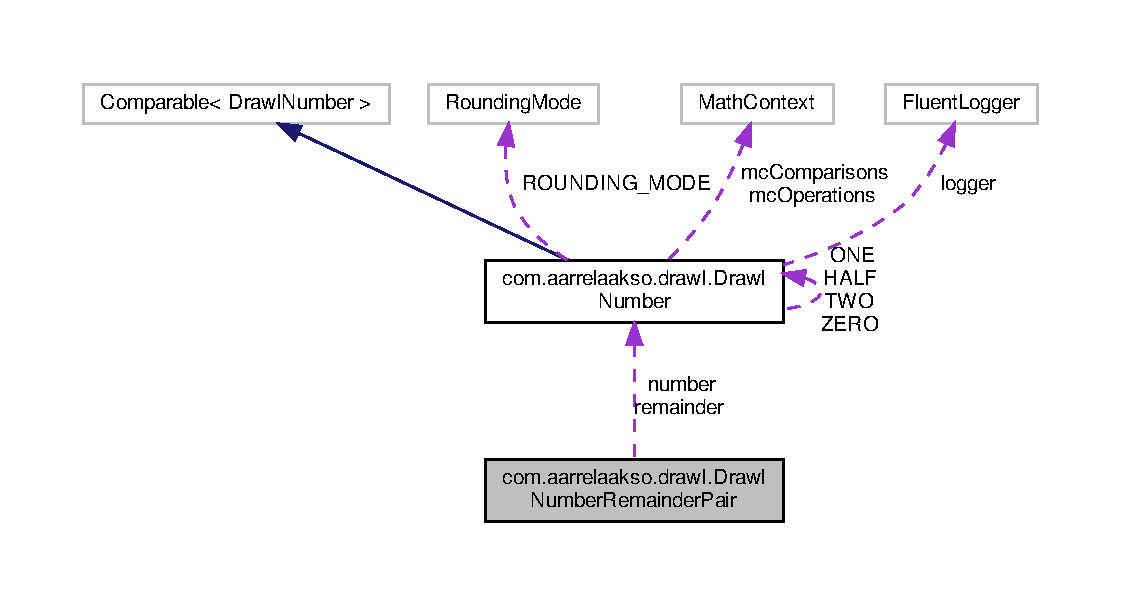
\includegraphics[width=350pt]{d9/dde/classcom_1_1aarrelaakso_1_1drawl_1_1_drawl_number_remainder_pair__coll__graph}
\end{center}
\end{figure}
\subsection*{Public Member Functions}
\begin{DoxyCompactItemize}
\item 
boolean \hyperlink{classcom_1_1aarrelaakso_1_1drawl_1_1_drawl_number_remainder_pair_ae619b9a18192478ece2b28978d892814}{equals} (Object obj)
\item 
\hyperlink{classcom_1_1aarrelaakso_1_1drawl_1_1_drawl_number}{Drawl\+Number} \hyperlink{classcom_1_1aarrelaakso_1_1drawl_1_1_drawl_number_remainder_pair_a0924839905a2c81b8bd4b2fd749e9783}{get\+Number} ()
\begin{DoxyCompactList}\small\item\em Returns number. \end{DoxyCompactList}\item 
\hyperlink{classcom_1_1aarrelaakso_1_1drawl_1_1_drawl_number}{Drawl\+Number} \hyperlink{classcom_1_1aarrelaakso_1_1drawl_1_1_drawl_number_remainder_pair_a1d30d70c9111a226e4dbf599139c7096}{get\+Remainder} ()
\begin{DoxyCompactList}\small\item\em Returns remainder. \end{DoxyCompactList}\item 
int \hyperlink{classcom_1_1aarrelaakso_1_1drawl_1_1_drawl_number_remainder_pair_aa56a76d72bd049756ea037819a8163fa}{hash\+Code} ()
\item 
String \hyperlink{classcom_1_1aarrelaakso_1_1drawl_1_1_drawl_number_remainder_pair_a4e2f7077149f0a6f6f4b66bb76a3feb0}{to\+String} ()
\end{DoxyCompactItemize}
\subsection*{Static Public Member Functions}
\begin{DoxyCompactItemize}
\item 
static \hyperlink{classcom_1_1aarrelaakso_1_1drawl_1_1_drawl_number_remainder_pair}{Drawl\+Number\+Remainder\+Pair} \hyperlink{classcom_1_1aarrelaakso_1_1drawl_1_1_drawl_number_remainder_pair_acf215ec7af4d8663e2cc0f6691b59d57}{value\+Of} (\hyperlink{classcom_1_1aarrelaakso_1_1drawl_1_1_drawl_number}{Drawl\+Number} \hyperlink{classcom_1_1aarrelaakso_1_1drawl_1_1_drawl_number_remainder_pair_a8c62602c155e6b1fe737605fe7229b36}{number}, \hyperlink{classcom_1_1aarrelaakso_1_1drawl_1_1_drawl_number}{Drawl\+Number} \hyperlink{classcom_1_1aarrelaakso_1_1drawl_1_1_drawl_number_remainder_pair_a95c7e55169d65822bbceb08ff2f800dc}{remainder})
\begin{DoxyCompactList}\small\item\em Creates new instance. \end{DoxyCompactList}\end{DoxyCompactItemize}
\subsection*{Private Member Functions}
\begin{DoxyCompactItemize}
\item 
\hyperlink{classcom_1_1aarrelaakso_1_1drawl_1_1_drawl_number_remainder_pair_aac59fe33b4a1888d48ba7bf4bc0ebaa4}{Drawl\+Number\+Remainder\+Pair} ()
\begin{DoxyCompactList}\small\item\em Creates new instance. \end{DoxyCompactList}\item 
void \hyperlink{classcom_1_1aarrelaakso_1_1drawl_1_1_drawl_number_remainder_pair_ae5c688bbfb072f385c338ab16f34c7a8}{guard\+Invariants} ()
\begin{DoxyCompactList}\small\item\em Guards this object to be consistent. \end{DoxyCompactList}\end{DoxyCompactItemize}
\subsection*{Private Attributes}
\begin{DoxyCompactItemize}
\item 
\hyperlink{classcom_1_1aarrelaakso_1_1drawl_1_1_drawl_number}{Drawl\+Number} \hyperlink{classcom_1_1aarrelaakso_1_1drawl_1_1_drawl_number_remainder_pair_a8c62602c155e6b1fe737605fe7229b36}{number}
\begin{DoxyCompactList}\small\item\em Unit number. \end{DoxyCompactList}\item 
\hyperlink{classcom_1_1aarrelaakso_1_1drawl_1_1_drawl_number}{Drawl\+Number} \hyperlink{classcom_1_1aarrelaakso_1_1drawl_1_1_drawl_number_remainder_pair_a95c7e55169d65822bbceb08ff2f800dc}{remainder}
\begin{DoxyCompactList}\small\item\em Remainder. \end{DoxyCompactList}\end{DoxyCompactItemize}


\subsection{Detailed Description}
Pair of the arbitrary number and remainder. 

This is the result after division operation.

\begin{DoxyAuthor}{Author}
radek.\+hecl 
\end{DoxyAuthor}


\subsection{Constructor \& Destructor Documentation}
\mbox{\Hypertarget{classcom_1_1aarrelaakso_1_1drawl_1_1_drawl_number_remainder_pair_aac59fe33b4a1888d48ba7bf4bc0ebaa4}\label{classcom_1_1aarrelaakso_1_1drawl_1_1_drawl_number_remainder_pair_aac59fe33b4a1888d48ba7bf4bc0ebaa4}} 
\index{com\+::aarrelaakso\+::drawl\+::\+Drawl\+Number\+Remainder\+Pair@{com\+::aarrelaakso\+::drawl\+::\+Drawl\+Number\+Remainder\+Pair}!Drawl\+Number\+Remainder\+Pair@{Drawl\+Number\+Remainder\+Pair}}
\index{Drawl\+Number\+Remainder\+Pair@{Drawl\+Number\+Remainder\+Pair}!com\+::aarrelaakso\+::drawl\+::\+Drawl\+Number\+Remainder\+Pair@{com\+::aarrelaakso\+::drawl\+::\+Drawl\+Number\+Remainder\+Pair}}
\subsubsection{\texorpdfstring{Drawl\+Number\+Remainder\+Pair()}{DrawlNumberRemainderPair()}}
{\footnotesize\ttfamily com.\+aarrelaakso.\+drawl.\+Drawl\+Number\+Remainder\+Pair.\+Drawl\+Number\+Remainder\+Pair (\begin{DoxyParamCaption}{ }\end{DoxyParamCaption})\hspace{0.3cm}{\ttfamily [private]}}



Creates new instance. 



\subsection{Member Function Documentation}
\mbox{\Hypertarget{classcom_1_1aarrelaakso_1_1drawl_1_1_drawl_number_remainder_pair_ae619b9a18192478ece2b28978d892814}\label{classcom_1_1aarrelaakso_1_1drawl_1_1_drawl_number_remainder_pair_ae619b9a18192478ece2b28978d892814}} 
\index{com\+::aarrelaakso\+::drawl\+::\+Drawl\+Number\+Remainder\+Pair@{com\+::aarrelaakso\+::drawl\+::\+Drawl\+Number\+Remainder\+Pair}!equals@{equals}}
\index{equals@{equals}!com\+::aarrelaakso\+::drawl\+::\+Drawl\+Number\+Remainder\+Pair@{com\+::aarrelaakso\+::drawl\+::\+Drawl\+Number\+Remainder\+Pair}}
\subsubsection{\texorpdfstring{equals()}{equals()}}
{\footnotesize\ttfamily boolean com.\+aarrelaakso.\+drawl.\+Drawl\+Number\+Remainder\+Pair.\+equals (\begin{DoxyParamCaption}\item[{Object}]{obj }\end{DoxyParamCaption})}

\mbox{\Hypertarget{classcom_1_1aarrelaakso_1_1drawl_1_1_drawl_number_remainder_pair_a0924839905a2c81b8bd4b2fd749e9783}\label{classcom_1_1aarrelaakso_1_1drawl_1_1_drawl_number_remainder_pair_a0924839905a2c81b8bd4b2fd749e9783}} 
\index{com\+::aarrelaakso\+::drawl\+::\+Drawl\+Number\+Remainder\+Pair@{com\+::aarrelaakso\+::drawl\+::\+Drawl\+Number\+Remainder\+Pair}!get\+Number@{get\+Number}}
\index{get\+Number@{get\+Number}!com\+::aarrelaakso\+::drawl\+::\+Drawl\+Number\+Remainder\+Pair@{com\+::aarrelaakso\+::drawl\+::\+Drawl\+Number\+Remainder\+Pair}}
\subsubsection{\texorpdfstring{get\+Number()}{getNumber()}}
{\footnotesize\ttfamily \hyperlink{classcom_1_1aarrelaakso_1_1drawl_1_1_drawl_number}{Drawl\+Number} com.\+aarrelaakso.\+drawl.\+Drawl\+Number\+Remainder\+Pair.\+get\+Number (\begin{DoxyParamCaption}{ }\end{DoxyParamCaption})}



Returns number. 

\begin{DoxyReturn}{Returns}
number 
\end{DoxyReturn}
\mbox{\Hypertarget{classcom_1_1aarrelaakso_1_1drawl_1_1_drawl_number_remainder_pair_a1d30d70c9111a226e4dbf599139c7096}\label{classcom_1_1aarrelaakso_1_1drawl_1_1_drawl_number_remainder_pair_a1d30d70c9111a226e4dbf599139c7096}} 
\index{com\+::aarrelaakso\+::drawl\+::\+Drawl\+Number\+Remainder\+Pair@{com\+::aarrelaakso\+::drawl\+::\+Drawl\+Number\+Remainder\+Pair}!get\+Remainder@{get\+Remainder}}
\index{get\+Remainder@{get\+Remainder}!com\+::aarrelaakso\+::drawl\+::\+Drawl\+Number\+Remainder\+Pair@{com\+::aarrelaakso\+::drawl\+::\+Drawl\+Number\+Remainder\+Pair}}
\subsubsection{\texorpdfstring{get\+Remainder()}{getRemainder()}}
{\footnotesize\ttfamily \hyperlink{classcom_1_1aarrelaakso_1_1drawl_1_1_drawl_number}{Drawl\+Number} com.\+aarrelaakso.\+drawl.\+Drawl\+Number\+Remainder\+Pair.\+get\+Remainder (\begin{DoxyParamCaption}{ }\end{DoxyParamCaption})}



Returns remainder. 

\begin{DoxyReturn}{Returns}
remainder 
\end{DoxyReturn}
\mbox{\Hypertarget{classcom_1_1aarrelaakso_1_1drawl_1_1_drawl_number_remainder_pair_ae5c688bbfb072f385c338ab16f34c7a8}\label{classcom_1_1aarrelaakso_1_1drawl_1_1_drawl_number_remainder_pair_ae5c688bbfb072f385c338ab16f34c7a8}} 
\index{com\+::aarrelaakso\+::drawl\+::\+Drawl\+Number\+Remainder\+Pair@{com\+::aarrelaakso\+::drawl\+::\+Drawl\+Number\+Remainder\+Pair}!guard\+Invariants@{guard\+Invariants}}
\index{guard\+Invariants@{guard\+Invariants}!com\+::aarrelaakso\+::drawl\+::\+Drawl\+Number\+Remainder\+Pair@{com\+::aarrelaakso\+::drawl\+::\+Drawl\+Number\+Remainder\+Pair}}
\subsubsection{\texorpdfstring{guard\+Invariants()}{guardInvariants()}}
{\footnotesize\ttfamily void com.\+aarrelaakso.\+drawl.\+Drawl\+Number\+Remainder\+Pair.\+guard\+Invariants (\begin{DoxyParamCaption}{ }\end{DoxyParamCaption})\hspace{0.3cm}{\ttfamily [private]}}



Guards this object to be consistent. 

Throws exception if this is not the case. \mbox{\Hypertarget{classcom_1_1aarrelaakso_1_1drawl_1_1_drawl_number_remainder_pair_aa56a76d72bd049756ea037819a8163fa}\label{classcom_1_1aarrelaakso_1_1drawl_1_1_drawl_number_remainder_pair_aa56a76d72bd049756ea037819a8163fa}} 
\index{com\+::aarrelaakso\+::drawl\+::\+Drawl\+Number\+Remainder\+Pair@{com\+::aarrelaakso\+::drawl\+::\+Drawl\+Number\+Remainder\+Pair}!hash\+Code@{hash\+Code}}
\index{hash\+Code@{hash\+Code}!com\+::aarrelaakso\+::drawl\+::\+Drawl\+Number\+Remainder\+Pair@{com\+::aarrelaakso\+::drawl\+::\+Drawl\+Number\+Remainder\+Pair}}
\subsubsection{\texorpdfstring{hash\+Code()}{hashCode()}}
{\footnotesize\ttfamily int com.\+aarrelaakso.\+drawl.\+Drawl\+Number\+Remainder\+Pair.\+hash\+Code (\begin{DoxyParamCaption}{ }\end{DoxyParamCaption})}

\mbox{\Hypertarget{classcom_1_1aarrelaakso_1_1drawl_1_1_drawl_number_remainder_pair_a4e2f7077149f0a6f6f4b66bb76a3feb0}\label{classcom_1_1aarrelaakso_1_1drawl_1_1_drawl_number_remainder_pair_a4e2f7077149f0a6f6f4b66bb76a3feb0}} 
\index{com\+::aarrelaakso\+::drawl\+::\+Drawl\+Number\+Remainder\+Pair@{com\+::aarrelaakso\+::drawl\+::\+Drawl\+Number\+Remainder\+Pair}!to\+String@{to\+String}}
\index{to\+String@{to\+String}!com\+::aarrelaakso\+::drawl\+::\+Drawl\+Number\+Remainder\+Pair@{com\+::aarrelaakso\+::drawl\+::\+Drawl\+Number\+Remainder\+Pair}}
\subsubsection{\texorpdfstring{to\+String()}{toString()}}
{\footnotesize\ttfamily String com.\+aarrelaakso.\+drawl.\+Drawl\+Number\+Remainder\+Pair.\+to\+String (\begin{DoxyParamCaption}{ }\end{DoxyParamCaption})}

\mbox{\Hypertarget{classcom_1_1aarrelaakso_1_1drawl_1_1_drawl_number_remainder_pair_acf215ec7af4d8663e2cc0f6691b59d57}\label{classcom_1_1aarrelaakso_1_1drawl_1_1_drawl_number_remainder_pair_acf215ec7af4d8663e2cc0f6691b59d57}} 
\index{com\+::aarrelaakso\+::drawl\+::\+Drawl\+Number\+Remainder\+Pair@{com\+::aarrelaakso\+::drawl\+::\+Drawl\+Number\+Remainder\+Pair}!value\+Of@{value\+Of}}
\index{value\+Of@{value\+Of}!com\+::aarrelaakso\+::drawl\+::\+Drawl\+Number\+Remainder\+Pair@{com\+::aarrelaakso\+::drawl\+::\+Drawl\+Number\+Remainder\+Pair}}
\subsubsection{\texorpdfstring{value\+Of()}{valueOf()}}
{\footnotesize\ttfamily static \hyperlink{classcom_1_1aarrelaakso_1_1drawl_1_1_drawl_number_remainder_pair}{Drawl\+Number\+Remainder\+Pair} com.\+aarrelaakso.\+drawl.\+Drawl\+Number\+Remainder\+Pair.\+value\+Of (\begin{DoxyParamCaption}\item[{\hyperlink{classcom_1_1aarrelaakso_1_1drawl_1_1_drawl_number}{Drawl\+Number}}]{number,  }\item[{\hyperlink{classcom_1_1aarrelaakso_1_1drawl_1_1_drawl_number}{Drawl\+Number}}]{remainder }\end{DoxyParamCaption})\hspace{0.3cm}{\ttfamily [static]}}



Creates new instance. 


\begin{DoxyParams}{Parameters}
{\em number} & number \\
\hline
{\em remainder} & remainder \\
\hline
\end{DoxyParams}
\begin{DoxyReturn}{Returns}
number remainder pair 
\end{DoxyReturn}


\subsection{Member Data Documentation}
\mbox{\Hypertarget{classcom_1_1aarrelaakso_1_1drawl_1_1_drawl_number_remainder_pair_a8c62602c155e6b1fe737605fe7229b36}\label{classcom_1_1aarrelaakso_1_1drawl_1_1_drawl_number_remainder_pair_a8c62602c155e6b1fe737605fe7229b36}} 
\index{com\+::aarrelaakso\+::drawl\+::\+Drawl\+Number\+Remainder\+Pair@{com\+::aarrelaakso\+::drawl\+::\+Drawl\+Number\+Remainder\+Pair}!number@{number}}
\index{number@{number}!com\+::aarrelaakso\+::drawl\+::\+Drawl\+Number\+Remainder\+Pair@{com\+::aarrelaakso\+::drawl\+::\+Drawl\+Number\+Remainder\+Pair}}
\subsubsection{\texorpdfstring{number}{number}}
{\footnotesize\ttfamily \hyperlink{classcom_1_1aarrelaakso_1_1drawl_1_1_drawl_number}{Drawl\+Number} com.\+aarrelaakso.\+drawl.\+Drawl\+Number\+Remainder\+Pair.\+number\hspace{0.3cm}{\ttfamily [private]}}



Unit number. 

\mbox{\Hypertarget{classcom_1_1aarrelaakso_1_1drawl_1_1_drawl_number_remainder_pair_a95c7e55169d65822bbceb08ff2f800dc}\label{classcom_1_1aarrelaakso_1_1drawl_1_1_drawl_number_remainder_pair_a95c7e55169d65822bbceb08ff2f800dc}} 
\index{com\+::aarrelaakso\+::drawl\+::\+Drawl\+Number\+Remainder\+Pair@{com\+::aarrelaakso\+::drawl\+::\+Drawl\+Number\+Remainder\+Pair}!remainder@{remainder}}
\index{remainder@{remainder}!com\+::aarrelaakso\+::drawl\+::\+Drawl\+Number\+Remainder\+Pair@{com\+::aarrelaakso\+::drawl\+::\+Drawl\+Number\+Remainder\+Pair}}
\subsubsection{\texorpdfstring{remainder}{remainder}}
{\footnotesize\ttfamily \hyperlink{classcom_1_1aarrelaakso_1_1drawl_1_1_drawl_number}{Drawl\+Number} com.\+aarrelaakso.\+drawl.\+Drawl\+Number\+Remainder\+Pair.\+remainder\hspace{0.3cm}{\ttfamily [private]}}



Remainder. 



The documentation for this class was generated from the following file\+:\begin{DoxyCompactItemize}
\item 
/mnt/d/\+One\+Drive/\+Documents/src/drawl/src/main/java/com/aarrelaakso/drawl/\hyperlink{_drawl_number_remainder_pair_8java}{Drawl\+Number\+Remainder\+Pair.\+java}\end{DoxyCompactItemize}

\hypertarget{classcom_1_1aarrelaakso_1_1drawl_1_1_line}{}\section{com.\+aarrelaakso.\+drawl.\+Line Class Reference}
\label{classcom_1_1aarrelaakso_1_1drawl_1_1_line}\index{com.\+aarrelaakso.\+drawl.\+Line@{com.\+aarrelaakso.\+drawl.\+Line}}


Represents lines.  


\subsection*{Classes}
\begin{DoxyCompactItemize}
\item 
enum \hyperlink{enumcom_1_1aarrelaakso_1_1drawl_1_1_line_1_1_orientation}{Orientation}
\begin{DoxyCompactList}\small\item\em How the line should be oriented. \end{DoxyCompactList}\end{DoxyCompactItemize}
\subsection*{Public Member Functions}
\begin{DoxyCompactItemize}
\item 
\hyperlink{classcom_1_1aarrelaakso_1_1drawl_1_1_line_af96a733c80d52bf419cab52fb09bc514}{Line} ()
\begin{DoxyCompactList}\small\item\em Constructs a default line whose ends are unknown. \end{DoxyCompactList}\item 
\hyperlink{classcom_1_1aarrelaakso_1_1drawl_1_1_line_aaeb9fdd60eeec26d881cb88a23c116b5}{Line} (\hyperlink{enumcom_1_1aarrelaakso_1_1drawl_1_1_line_1_1_orientation}{Orientation} \hyperlink{classcom_1_1aarrelaakso_1_1drawl_1_1_line_a441ce546831b219e01f5fd0f7e0bb3b1}{orientation})
\begin{DoxyCompactList}\small\item\em Constructs a line at a particular orientation. \end{DoxyCompactList}\item 
\hyperlink{classcom_1_1aarrelaakso_1_1drawl_1_1_line_a9e956655eba16543d82728923c3eb4f6}{Line} (@Not\+Null final \hyperlink{classcom_1_1aarrelaakso_1_1drawl_1_1_point}{Point} \hyperlink{classcom_1_1aarrelaakso_1_1drawl_1_1_line_a48220286707ae05387f9c99d9e08784c}{point1\+Implicit}, @Not\+Null final \hyperlink{classcom_1_1aarrelaakso_1_1drawl_1_1_point}{Point} \hyperlink{classcom_1_1aarrelaakso_1_1drawl_1_1_line_a055d1e743c66cc808f108664b38d7de2}{point2\+Implicit})
\begin{DoxyCompactList}\small\item\em Constructs a line from one point to another. \end{DoxyCompactList}\item 
void \hyperlink{classcom_1_1aarrelaakso_1_1drawl_1_1_line_a7c54922855fda2590c962ac8e03c220c}{add\+Arrowhead} (final \hyperlink{classcom_1_1aarrelaakso_1_1drawl_1_1_arrowhead}{Arrowhead} \hyperlink{classcom_1_1aarrelaakso_1_1drawl_1_1_line_a6a82ee992a758049f71dfbb22c597149}{lineEnding})
\item 
String \hyperlink{classcom_1_1aarrelaakso_1_1drawl_1_1_line_a6a54dd70515b691c8afa88f980e10698}{get\+S\+VG} ()
\item 
void \hyperlink{classcom_1_1aarrelaakso_1_1drawl_1_1_line_af58511076072e05cf42641ee44d0d0d7}{set\+Thickness} (double \hyperlink{classcom_1_1aarrelaakso_1_1drawl_1_1_line_a314ae0371f5665cf70ad99742d44934a}{thickness})
\item 
double \hyperlink{classcom_1_1aarrelaakso_1_1drawl_1_1_line_aa25b4985b90dd7ebad4cbdc403f22a42}{get\+Thickness} ()
\item 
boolean \hyperlink{classcom_1_1aarrelaakso_1_1drawl_1_1_line_a422ac149cee14f3123989e44477d78d2}{has\+Arrowhead} ()
\item 
void \hyperlink{classcom_1_1aarrelaakso_1_1drawl_1_1_shape_af6fea9610721de462c18ee640043aba7}{add\+Text} (@Nullable final \hyperlink{classcom_1_1aarrelaakso_1_1drawl_1_1_text}{Text} \hyperlink{classcom_1_1aarrelaakso_1_1drawl_1_1_shape_ab54afc2d95d3447532f5ecf3fec3faa8}{text})
\begin{DoxyCompactList}\small\item\em Adds \hyperlink{classcom_1_1aarrelaakso_1_1drawl_1_1_text}{Text} inside this \hyperlink{classcom_1_1aarrelaakso_1_1drawl_1_1_shape}{Shape}. \end{DoxyCompactList}\item 
\hyperlink{classcom_1_1aarrelaakso_1_1drawl_1_1_shape}{Shape} \hyperlink{classcom_1_1aarrelaakso_1_1drawl_1_1_shape_acebea2aa57031322323c9bf50ee447db}{get\+Above} ()
\begin{DoxyCompactList}\small\item\em Gets this \hyperlink{classcom_1_1aarrelaakso_1_1drawl_1_1_shape}{Shape}\textquotesingle{}s neighbor above (this \hyperlink{classcom_1_1aarrelaakso_1_1drawl_1_1_shape}{Shape} is below that one), if any. \end{DoxyCompactList}\item 
void \hyperlink{classcom_1_1aarrelaakso_1_1drawl_1_1_shape_a4deb22d64fef2115a0bc4802e8dba682}{set\+Above} (@Not\+Null final \hyperlink{classcom_1_1aarrelaakso_1_1drawl_1_1_shape}{Shape} shape)
\begin{DoxyCompactList}\small\item\em Sets this \hyperlink{classcom_1_1aarrelaakso_1_1drawl_1_1_shape}{Shape} above another \hyperlink{classcom_1_1aarrelaakso_1_1drawl_1_1_shape}{Shape}. \end{DoxyCompactList}\item 
void \hyperlink{classcom_1_1aarrelaakso_1_1drawl_1_1_shape_aad0b2fb173c0112b71b06cf90709acc3}{set\+Above} (@Not\+Null final \hyperlink{classcom_1_1aarrelaakso_1_1drawl_1_1_shape}{Shape} shape, @Not\+Null final \hyperlink{classcom_1_1aarrelaakso_1_1drawl_1_1_measure}{Measure} offset)
\begin{DoxyCompactList}\small\item\em Sets this \hyperlink{classcom_1_1aarrelaakso_1_1drawl_1_1_shape}{Shape} above another \hyperlink{classcom_1_1aarrelaakso_1_1drawl_1_1_shape}{Shape}. \end{DoxyCompactList}\item 
\hyperlink{classcom_1_1aarrelaakso_1_1drawl_1_1_shape}{Shape} \hyperlink{classcom_1_1aarrelaakso_1_1drawl_1_1_shape_a53de5ab609d879719cd3b372dfe8df58}{get\+Below} ()
\begin{DoxyCompactList}\small\item\em Gets this \hyperlink{classcom_1_1aarrelaakso_1_1drawl_1_1_shape}{Shape}\textquotesingle{}s neighbor below (this \hyperlink{classcom_1_1aarrelaakso_1_1drawl_1_1_shape}{Shape} is above that one), if any. \end{DoxyCompactList}\item 
void \hyperlink{classcom_1_1aarrelaakso_1_1drawl_1_1_shape_a4147526667449f5beb534d4404ba8f77}{set\+Below} (@Not\+Null final \hyperlink{classcom_1_1aarrelaakso_1_1drawl_1_1_shape}{Shape} shape)
\begin{DoxyCompactList}\small\item\em Sets this \hyperlink{classcom_1_1aarrelaakso_1_1drawl_1_1_shape}{Shape} below another \hyperlink{classcom_1_1aarrelaakso_1_1drawl_1_1_shape}{Shape}. \end{DoxyCompactList}\item 
void \hyperlink{classcom_1_1aarrelaakso_1_1drawl_1_1_shape_a63c902c4e79235901744c6d83544fa54}{set\+Below} (@Not\+Null final \hyperlink{classcom_1_1aarrelaakso_1_1drawl_1_1_shape}{Shape} shape, @Not\+Null final \hyperlink{classcom_1_1aarrelaakso_1_1drawl_1_1_measure}{Measure} offset)
\begin{DoxyCompactList}\small\item\em Sets this circle below another circle. \end{DoxyCompactList}\item 
\hyperlink{classcom_1_1aarrelaakso_1_1drawl_1_1_point}{Point} \hyperlink{classcom_1_1aarrelaakso_1_1drawl_1_1_shape_aba14efe9a16c0808580963c66b171082}{get\+Bottom\+Port} ()
\begin{DoxyCompactList}\small\item\em Returns a \hyperlink{classcom_1_1aarrelaakso_1_1drawl_1_1_point}{Point} object representing this \hyperlink{classcom_1_1aarrelaakso_1_1drawl_1_1_shape}{Shape}\textquotesingle{}s bottom port. \end{DoxyCompactList}\item 
String \hyperlink{classcom_1_1aarrelaakso_1_1drawl_1_1_shape_a0d9a33a3e151aaceeec140bea343a650}{get\+Fill} ()
\begin{DoxyCompactList}\small\item\em Returns the fill associated with this \hyperlink{classcom_1_1aarrelaakso_1_1drawl_1_1_shape}{Shape}, if any. \end{DoxyCompactList}\item 
void \hyperlink{classcom_1_1aarrelaakso_1_1drawl_1_1_shape_a81ff4feb49b8f74c1a639564748a23ee}{set\+Fill} (final String s)
\begin{DoxyCompactList}\small\item\em Set the fill of this \hyperlink{classcom_1_1aarrelaakso_1_1drawl_1_1_shape}{Shape}. \end{DoxyCompactList}\item 
\hyperlink{classcom_1_1aarrelaakso_1_1drawl_1_1_measure}{Measure} \hyperlink{classcom_1_1aarrelaakso_1_1drawl_1_1_shape_ac9f74d31c332aab76b329edc22080e67}{get\+Height} ()
\begin{DoxyCompactList}\small\item\em Returns a \hyperlink{classcom_1_1aarrelaakso_1_1drawl_1_1_measure}{Measure} object that represents the height of this \hyperlink{classcom_1_1aarrelaakso_1_1drawl_1_1_shape}{Shape}. \end{DoxyCompactList}\item 
\hyperlink{classcom_1_1aarrelaakso_1_1drawl_1_1_shape}{Shape} \hyperlink{classcom_1_1aarrelaakso_1_1drawl_1_1_shape_a2b19d5964ac46d545a7bae3133df6532}{get\+Left\+Of} ()
\begin{DoxyCompactList}\small\item\em Gets this \hyperlink{classcom_1_1aarrelaakso_1_1drawl_1_1_shape}{Shape}\textquotesingle{}s neighbor to the right (this \hyperlink{classcom_1_1aarrelaakso_1_1drawl_1_1_shape}{Shape} is to the left of that one), if any. \end{DoxyCompactList}\item 
void \hyperlink{classcom_1_1aarrelaakso_1_1drawl_1_1_shape_a0aef56392d76202235a9520394e87492}{set\+Left\+Of} (@Not\+Null final \hyperlink{classcom_1_1aarrelaakso_1_1drawl_1_1_shape}{Shape} shape)
\begin{DoxyCompactList}\small\item\em Sets this \hyperlink{classcom_1_1aarrelaakso_1_1drawl_1_1_shape}{Shape} to the left of another one. \end{DoxyCompactList}\item 
void \hyperlink{classcom_1_1aarrelaakso_1_1drawl_1_1_shape_a8012a3823982d77b563ef61787ccb523}{set\+Left\+Of} (@Not\+Null final \hyperlink{classcom_1_1aarrelaakso_1_1drawl_1_1_shape}{Shape} shape, @Not\+Null final \hyperlink{classcom_1_1aarrelaakso_1_1drawl_1_1_measure}{Measure} offset)
\begin{DoxyCompactList}\small\item\em Sets this \hyperlink{classcom_1_1aarrelaakso_1_1drawl_1_1_shape}{Shape}\textquotesingle{}s neighbor to the right (this \hyperlink{classcom_1_1aarrelaakso_1_1drawl_1_1_shape}{Shape} is to the left of that one). \end{DoxyCompactList}\item 
\hyperlink{classcom_1_1aarrelaakso_1_1drawl_1_1_point}{Point} \hyperlink{classcom_1_1aarrelaakso_1_1drawl_1_1_shape_aeffa96786ca552adf46924ec77da9555}{get\+Left\+Port} ()
\begin{DoxyCompactList}\small\item\em Returns a \hyperlink{classcom_1_1aarrelaakso_1_1drawl_1_1_point}{Point} object representing this \hyperlink{classcom_1_1aarrelaakso_1_1drawl_1_1_shape}{Shape}\textquotesingle{}s left port. \end{DoxyCompactList}\item 
\hyperlink{classcom_1_1aarrelaakso_1_1drawl_1_1_shape}{Shape} \hyperlink{classcom_1_1aarrelaakso_1_1drawl_1_1_shape_a1ad573b06f341aa79f6a255a476ae6e4}{get\+Right\+Of} ()
\begin{DoxyCompactList}\small\item\em Gets this \hyperlink{classcom_1_1aarrelaakso_1_1drawl_1_1_shape}{Shape}\textquotesingle{}s neighbor to the left (this \hyperlink{classcom_1_1aarrelaakso_1_1drawl_1_1_shape}{Shape} is to the right of that one), if any. \end{DoxyCompactList}\item 
void \hyperlink{classcom_1_1aarrelaakso_1_1drawl_1_1_shape_a3cada5e03bd1552a79702d2945c7ed01}{set\+Right\+Of} (@Not\+Null final \hyperlink{classcom_1_1aarrelaakso_1_1drawl_1_1_shape}{Shape} shape)
\begin{DoxyCompactList}\small\item\em Sets this \hyperlink{classcom_1_1aarrelaakso_1_1drawl_1_1_shape}{Shape}\textquotesingle{}s neighbor to the left (this \hyperlink{classcom_1_1aarrelaakso_1_1drawl_1_1_shape}{Shape} is to the right of that one). \end{DoxyCompactList}\item 
void \hyperlink{classcom_1_1aarrelaakso_1_1drawl_1_1_shape_a89e85848d24dca0fa60ff68d169eef11}{set\+Right\+Of} (@Not\+Null final \hyperlink{classcom_1_1aarrelaakso_1_1drawl_1_1_shape}{Shape} shape, @Not\+Null final \hyperlink{classcom_1_1aarrelaakso_1_1drawl_1_1_measure}{Measure} offset)
\begin{DoxyCompactList}\small\item\em Sets this \hyperlink{classcom_1_1aarrelaakso_1_1drawl_1_1_shape}{Shape}\textquotesingle{}s neighbor to the left with an offset. \end{DoxyCompactList}\item 
\hyperlink{classcom_1_1aarrelaakso_1_1drawl_1_1_point}{Point} \hyperlink{classcom_1_1aarrelaakso_1_1drawl_1_1_shape_a319c78d425ec91e1aef1072a95e349ad}{get\+Right\+Port} ()
\begin{DoxyCompactList}\small\item\em Returns a \hyperlink{classcom_1_1aarrelaakso_1_1drawl_1_1_point}{Point} object representing this \hyperlink{classcom_1_1aarrelaakso_1_1drawl_1_1_shape}{Shape}\textquotesingle{}s left port. \end{DoxyCompactList}\item 
String \hyperlink{classcom_1_1aarrelaakso_1_1drawl_1_1_shape_a4e1d54c7e161e3af5053939ddefdf9e6}{get\+Stroke} ()
\begin{DoxyCompactList}\small\item\em Gets the stroke of this \hyperlink{classcom_1_1aarrelaakso_1_1drawl_1_1_shape}{Shape}. \end{DoxyCompactList}\item 
void \hyperlink{classcom_1_1aarrelaakso_1_1drawl_1_1_shape_a75685cbfea36858836df8e1fb4f8b821}{set\+Stroke} (final String s)
\begin{DoxyCompactList}\small\item\em Sets the stroke of this shape. \end{DoxyCompactList}\item 
\hyperlink{classcom_1_1aarrelaakso_1_1drawl_1_1_text}{Text} \hyperlink{classcom_1_1aarrelaakso_1_1drawl_1_1_shape_a6f876978d4102974fedc5b41c93c7b26}{get\+Text} ()
\begin{DoxyCompactList}\small\item\em Returns a \hyperlink{classcom_1_1aarrelaakso_1_1drawl_1_1_text}{Text} object that belongs to this \hyperlink{classcom_1_1aarrelaakso_1_1drawl_1_1_shape}{Shape}, if there is one. \end{DoxyCompactList}\item 
\hyperlink{classcom_1_1aarrelaakso_1_1drawl_1_1_point}{Point} \hyperlink{classcom_1_1aarrelaakso_1_1drawl_1_1_shape_aed4e9caa294aacc973b7a531a960e9e5}{get\+Top\+Port} ()
\begin{DoxyCompactList}\small\item\em Returns a \hyperlink{classcom_1_1aarrelaakso_1_1drawl_1_1_point}{Point} object representing this \hyperlink{classcom_1_1aarrelaakso_1_1drawl_1_1_shape}{Shape}\textquotesingle{}s top port. \end{DoxyCompactList}\item 
void \hyperlink{classcom_1_1aarrelaakso_1_1drawl_1_1_shape_a8b5f19ff40445c0cf8cad2688d7df810}{set\+Width} (\hyperlink{classcom_1_1aarrelaakso_1_1drawl_1_1_measure}{Measure} width)
\begin{DoxyCompactList}\small\item\em Sets the width of this object. \end{DoxyCompactList}\item 
\hyperlink{classcom_1_1aarrelaakso_1_1drawl_1_1_measure}{Measure} \hyperlink{classcom_1_1aarrelaakso_1_1drawl_1_1_shape_a3e2c58984f1bcbc2e9e86cf30868561e}{get\+Width} ()
\begin{DoxyCompactList}\small\item\em Returns a \hyperlink{classcom_1_1aarrelaakso_1_1drawl_1_1_measure}{Measure} object that represents the width of this \hyperlink{classcom_1_1aarrelaakso_1_1drawl_1_1_shape}{Shape}. \end{DoxyCompactList}\item 
Boolean \hyperlink{classcom_1_1aarrelaakso_1_1drawl_1_1_shape_a037a5515b2a6e1df1d1981aa5516e78e}{has\+Text} ()
\begin{DoxyCompactList}\small\item\em Indicates whether this shape has a \hyperlink{classcom_1_1aarrelaakso_1_1drawl_1_1_text}{Text} object associated with it. \end{DoxyCompactList}\end{DoxyCompactItemize}
\subsection*{Protected Member Functions}
\begin{DoxyCompactItemize}
\item 
\hyperlink{classcom_1_1aarrelaakso_1_1drawl_1_1_point}{Point} \hyperlink{classcom_1_1aarrelaakso_1_1drawl_1_1_line_ac8344112f3a5d24cfa4b732f3625af08}{get\+Point1\+Explicit} ()
\item 
\hyperlink{classcom_1_1aarrelaakso_1_1drawl_1_1_point}{Point} \hyperlink{classcom_1_1aarrelaakso_1_1drawl_1_1_line_a1f2be99b388cc8bfb6f2bb866c21138f}{get\+Point2\+Explicit} ()
\item 
\hyperlink{classcom_1_1aarrelaakso_1_1drawl_1_1_point}{Point} \hyperlink{classcom_1_1aarrelaakso_1_1drawl_1_1_line_a687f4da61c3f8760840713ff2da6ecaa}{get\+Point1\+Implicit} ()
\item 
\hyperlink{classcom_1_1aarrelaakso_1_1drawl_1_1_point}{Point} \hyperlink{classcom_1_1aarrelaakso_1_1drawl_1_1_line_a275e3535223921a66570a24d8a648586}{get\+Point2\+Implicit} ()
\item 
\hyperlink{interfacecom_1_1aarrelaakso_1_1drawl_1_1_number}{Number} \hyperlink{classcom_1_1aarrelaakso_1_1drawl_1_1_shape_a3acdc2fd1944e2efacd0bfbb8aefe89b}{get\+Explicit\+Half\+Width} ()
\begin{DoxyCompactList}\small\item\em Gets half the explicit width of this \hyperlink{classcom_1_1aarrelaakso_1_1drawl_1_1_shape}{Shape}. \end{DoxyCompactList}\item 
\hyperlink{interfacecom_1_1aarrelaakso_1_1drawl_1_1_number}{Number} \hyperlink{classcom_1_1aarrelaakso_1_1drawl_1_1_shape_a48917787cedbfd447cd37edbb59a1145}{get\+Explicit\+Height} ()
\begin{DoxyCompactList}\small\item\em Get the explicit height of this \hyperlink{classcom_1_1aarrelaakso_1_1drawl_1_1_shape}{Shape}. \end{DoxyCompactList}\item 
void \hyperlink{classcom_1_1aarrelaakso_1_1drawl_1_1_shape_a3680a63cef0d766132d1f64813ca8eca}{set\+Explicit\+Height} (@Nullable final \hyperlink{interfacecom_1_1aarrelaakso_1_1drawl_1_1_number}{Number} height)
\begin{DoxyCompactList}\small\item\em Set the height of this \hyperlink{classcom_1_1aarrelaakso_1_1drawl_1_1_shape}{Shape} to an explicit value. \end{DoxyCompactList}\item 
\hyperlink{interfacecom_1_1aarrelaakso_1_1drawl_1_1_number}{Number} \hyperlink{classcom_1_1aarrelaakso_1_1drawl_1_1_shape_aca08f18bbe102a5cf6a77cb746d42875}{get\+Explicit\+Width} ()
\begin{DoxyCompactList}\small\item\em Get the explicit width of this \hyperlink{classcom_1_1aarrelaakso_1_1drawl_1_1_shape}{Shape}. \end{DoxyCompactList}\item 
void \hyperlink{classcom_1_1aarrelaakso_1_1drawl_1_1_shape_a386685477bfc007aab782565f140265d}{set\+Explicit\+Width} (@Nullable final \hyperlink{interfacecom_1_1aarrelaakso_1_1drawl_1_1_number}{Number} width)
\begin{DoxyCompactList}\small\item\em Set the width of this \hyperlink{classcom_1_1aarrelaakso_1_1drawl_1_1_shape}{Shape} to an explicit value. \end{DoxyCompactList}\item 
\hyperlink{interfacecom_1_1aarrelaakso_1_1drawl_1_1_number}{Number} \hyperlink{classcom_1_1aarrelaakso_1_1drawl_1_1_shape_aa1fbd5a290bc5d2df437f0bd79f30a89}{get\+Explicit\+X\+Position\+Center} ()
\begin{DoxyCompactList}\small\item\em Gets the explicit x-\/position of the center of this \hyperlink{classcom_1_1aarrelaakso_1_1drawl_1_1_shape}{Shape}. \end{DoxyCompactList}\item 
void \hyperlink{classcom_1_1aarrelaakso_1_1drawl_1_1_shape_a28c766b414be0cd8767093f9be557dbd}{set\+Explicit\+X\+Position\+Center} (final \hyperlink{interfacecom_1_1aarrelaakso_1_1drawl_1_1_number}{Number} x)
\begin{DoxyCompactList}\small\item\em Sets the explicit center position of this \hyperlink{classcom_1_1aarrelaakso_1_1drawl_1_1_shape}{Shape}. \end{DoxyCompactList}\item 
void \hyperlink{classcom_1_1aarrelaakso_1_1drawl_1_1_shape_a271cd9377952616a30a434b22e22000a}{set\+Explicit\+X\+Position\+Center} (final Integer x)
\begin{DoxyCompactList}\small\item\em Sets the explicit x position of the center of this \hyperlink{classcom_1_1aarrelaakso_1_1drawl_1_1_shape}{Shape}. \end{DoxyCompactList}\item 
\hyperlink{interfacecom_1_1aarrelaakso_1_1drawl_1_1_number}{Number} \hyperlink{classcom_1_1aarrelaakso_1_1drawl_1_1_shape_abd7f6c77e2c62100bb72d8ad3085e288}{get\+Explicit\+X\+Position\+Left} ()
\begin{DoxyCompactList}\small\item\em Gets the explicit x position of the left edge of this \hyperlink{classcom_1_1aarrelaakso_1_1drawl_1_1_shape}{Shape}. \end{DoxyCompactList}\item 
\hyperlink{interfacecom_1_1aarrelaakso_1_1drawl_1_1_number}{Number} \hyperlink{classcom_1_1aarrelaakso_1_1drawl_1_1_shape_a86920ba43a76d5a02977e5f9ea3509ac}{get\+Explicit\+X\+Position\+Right} ()
\begin{DoxyCompactList}\small\item\em Gets the explicit x position of the right edge of this \hyperlink{classcom_1_1aarrelaakso_1_1drawl_1_1_shape}{Shape}. \end{DoxyCompactList}\item 
\hyperlink{interfacecom_1_1aarrelaakso_1_1drawl_1_1_number}{Number} \hyperlink{classcom_1_1aarrelaakso_1_1drawl_1_1_shape_a28b8e03381be6afdc7c5c8da48c80afe}{get\+Explicit\+Y\+Position\+Bottom} ()
\begin{DoxyCompactList}\small\item\em Gets the explicit y position of the bottom of this \hyperlink{classcom_1_1aarrelaakso_1_1drawl_1_1_shape}{Shape}. \end{DoxyCompactList}\item 
\hyperlink{interfacecom_1_1aarrelaakso_1_1drawl_1_1_number}{Number} \hyperlink{classcom_1_1aarrelaakso_1_1drawl_1_1_shape_a1e46cc626d5f5e1360d9d35d23cc50ea}{get\+Explicit\+Y\+Position\+Center} ()
\begin{DoxyCompactList}\small\item\em Gets the explicit y-\/position of the center of this \hyperlink{classcom_1_1aarrelaakso_1_1drawl_1_1_shape}{Shape}. \end{DoxyCompactList}\item 
void \hyperlink{classcom_1_1aarrelaakso_1_1drawl_1_1_shape_a93e9e1bdd05f111661660e9de621cd12}{set\+Explicit\+Y\+Position\+Center} (final Integer y)
\begin{DoxyCompactList}\small\item\em Sets the explicit y-\/position of the center of this \hyperlink{classcom_1_1aarrelaakso_1_1drawl_1_1_shape}{Shape}. \end{DoxyCompactList}\item 
void \hyperlink{classcom_1_1aarrelaakso_1_1drawl_1_1_shape_a7d49d69bd74e57c3a3341a025c3cce50}{set\+Explicit\+Y\+Position\+Center} (final \hyperlink{interfacecom_1_1aarrelaakso_1_1drawl_1_1_number}{Number} y)
\begin{DoxyCompactList}\small\item\em Sets the explicit y position of this \hyperlink{classcom_1_1aarrelaakso_1_1drawl_1_1_shape}{Shape}. \end{DoxyCompactList}\item 
\hyperlink{interfacecom_1_1aarrelaakso_1_1drawl_1_1_number}{Number} \hyperlink{classcom_1_1aarrelaakso_1_1drawl_1_1_shape_a8c65dff2026744ae10648de3908165e5}{get\+Explicit\+Y\+Position\+Top} ()
\begin{DoxyCompactList}\small\item\em Gets the explicit y-\/position of the top of this \hyperlink{classcom_1_1aarrelaakso_1_1drawl_1_1_shape}{Shape}. \end{DoxyCompactList}\item 
\hyperlink{interfacecom_1_1aarrelaakso_1_1drawl_1_1_number}{Number} \hyperlink{classcom_1_1aarrelaakso_1_1drawl_1_1_shape_a4af0fd7e309ea01bced73076510ef897}{get\+Implicit\+Half\+Height} ()
\begin{DoxyCompactList}\small\item\em Gets half of the implicit height of this \hyperlink{classcom_1_1aarrelaakso_1_1drawl_1_1_shape}{Shape}. \end{DoxyCompactList}\item 
\hyperlink{interfacecom_1_1aarrelaakso_1_1drawl_1_1_number}{Number} \hyperlink{classcom_1_1aarrelaakso_1_1drawl_1_1_shape_a02d73887a309bcd1178b142ad0c7edd9}{get\+Implicit\+Half\+Width} ()
\begin{DoxyCompactList}\small\item\em Gets half of the implicit width of this \hyperlink{classcom_1_1aarrelaakso_1_1drawl_1_1_shape}{Shape}. \end{DoxyCompactList}\item 
\hyperlink{interfacecom_1_1aarrelaakso_1_1drawl_1_1_number}{Number} \hyperlink{classcom_1_1aarrelaakso_1_1drawl_1_1_shape_a3b0ad73b41fe8c9ae66d20f7fc1de7c9}{get\+Implicit\+Height} ()
\begin{DoxyCompactList}\small\item\em Gets the implicit height of this \hyperlink{classcom_1_1aarrelaakso_1_1drawl_1_1_shape}{Shape}. \end{DoxyCompactList}\item 
final void \hyperlink{classcom_1_1aarrelaakso_1_1drawl_1_1_shape_a608e72be0fb16380e5fda14564c46739}{set\+Implicit\+Height} (@Not\+Null final \hyperlink{interfacecom_1_1aarrelaakso_1_1drawl_1_1_number}{Number} \hyperlink{classcom_1_1aarrelaakso_1_1drawl_1_1_shape_a9270317569c41e7f3f3fbe6e71df86e6}{implicit\+Height})
\begin{DoxyCompactList}\small\item\em Sets the implicit height of this \hyperlink{classcom_1_1aarrelaakso_1_1drawl_1_1_shape}{Shape}. \end{DoxyCompactList}\item 
\hyperlink{interfacecom_1_1aarrelaakso_1_1drawl_1_1_number}{Number} \hyperlink{classcom_1_1aarrelaakso_1_1drawl_1_1_shape_af8182545b3b1c85ecaee849474f63c6b}{get\+Implicit\+Width} ()
\begin{DoxyCompactList}\small\item\em Gets the implicit width of this \hyperlink{classcom_1_1aarrelaakso_1_1drawl_1_1_shape}{Shape}. \end{DoxyCompactList}\item 
final void \hyperlink{classcom_1_1aarrelaakso_1_1drawl_1_1_shape_acc3e365064b5d4f719ac920a5a70aedb}{set\+Implicit\+Width} (@Not\+Null final \hyperlink{interfacecom_1_1aarrelaakso_1_1drawl_1_1_number}{Number} \hyperlink{classcom_1_1aarrelaakso_1_1drawl_1_1_shape_a06c9063aa0b51139910e23414428c9d6}{implicit\+Width})
\begin{DoxyCompactList}\small\item\em Sets the implicit width of this \hyperlink{classcom_1_1aarrelaakso_1_1drawl_1_1_shape}{Shape}. \end{DoxyCompactList}\item 
\hyperlink{interfacecom_1_1aarrelaakso_1_1drawl_1_1_number}{Number} \hyperlink{classcom_1_1aarrelaakso_1_1drawl_1_1_shape_a0903079fd35e3cfdd6cdc299548a9680}{get\+Implicit\+X\+Maximum} ()
\begin{DoxyCompactList}\small\item\em Get the implicit maximum (rightmost) x-\/position of this \hyperlink{classcom_1_1aarrelaakso_1_1drawl_1_1_shape}{Shape}. \end{DoxyCompactList}\item 
\hyperlink{interfacecom_1_1aarrelaakso_1_1drawl_1_1_number}{Number} \hyperlink{classcom_1_1aarrelaakso_1_1drawl_1_1_shape_a264da8a94218b09267c2e177ff0b0951}{get\+Implicit\+X\+Minimum} ()
\begin{DoxyCompactList}\small\item\em Get the implicit minimum (leftmost) x-\/position of this \hyperlink{classcom_1_1aarrelaakso_1_1drawl_1_1_shape}{Shape}. \end{DoxyCompactList}\item 
\hyperlink{interfacecom_1_1aarrelaakso_1_1drawl_1_1_number}{Number} \hyperlink{classcom_1_1aarrelaakso_1_1drawl_1_1_shape_a9632097be62eb03e09145763852bda85}{get\+Implicit\+X\+Position\+Center} ()
\begin{DoxyCompactList}\small\item\em Get the implicit x position of the center of this \hyperlink{classcom_1_1aarrelaakso_1_1drawl_1_1_shape}{Shape}. \end{DoxyCompactList}\item 
void \hyperlink{classcom_1_1aarrelaakso_1_1drawl_1_1_shape_a945597709a9d79688e48a9802c86b13b}{set\+Implicit\+X\+Position\+Center} (final \hyperlink{interfacecom_1_1aarrelaakso_1_1drawl_1_1_number}{Number} x)
\begin{DoxyCompactList}\small\item\em Sets the implicit x position of the center of this \hyperlink{classcom_1_1aarrelaakso_1_1drawl_1_1_shape}{Shape}. \end{DoxyCompactList}\item 
\hyperlink{interfacecom_1_1aarrelaakso_1_1drawl_1_1_number}{Number} \hyperlink{classcom_1_1aarrelaakso_1_1drawl_1_1_shape_a2f272e8bfa625bb7959d1f722d5ac3df}{get\+Implicit\+X\+Position\+Left} ()
\begin{DoxyCompactList}\small\item\em Gets the implicit x position of the left edge of this \hyperlink{classcom_1_1aarrelaakso_1_1drawl_1_1_shape}{Shape}. \end{DoxyCompactList}\item 
\hyperlink{interfacecom_1_1aarrelaakso_1_1drawl_1_1_number}{Number} \hyperlink{classcom_1_1aarrelaakso_1_1drawl_1_1_shape_a15599ef4ee30a0ddd372f7cf1b155ce1}{get\+Implicit\+X\+Position\+Right} ()
\begin{DoxyCompactList}\small\item\em Gets the implicit x position of the right edge of this \hyperlink{classcom_1_1aarrelaakso_1_1drawl_1_1_shape}{Shape}. \end{DoxyCompactList}\item 
\hyperlink{interfacecom_1_1aarrelaakso_1_1drawl_1_1_number}{Number} \hyperlink{classcom_1_1aarrelaakso_1_1drawl_1_1_shape_a8d44b02976656bf4a81055a2dbae66cb}{get\+Implicit\+Y\+Position\+Bottom} ()
\begin{DoxyCompactList}\small\item\em Gets the implicit bottommost y-\/position of this \hyperlink{classcom_1_1aarrelaakso_1_1drawl_1_1_shape}{Shape}. \end{DoxyCompactList}\item 
\hyperlink{interfacecom_1_1aarrelaakso_1_1drawl_1_1_number}{Number} \hyperlink{classcom_1_1aarrelaakso_1_1drawl_1_1_shape_a1f27f0adc1716dc60691a7d0c14f2ace}{get\+Implicit\+Y\+Position\+Center} ()
\begin{DoxyCompactList}\small\item\em Gets the implicit y position of the center of this \hyperlink{classcom_1_1aarrelaakso_1_1drawl_1_1_shape}{Shape}. \end{DoxyCompactList}\item 
void \hyperlink{classcom_1_1aarrelaakso_1_1drawl_1_1_shape_a79c79420c626b8b2d2534b6c9aa64d8f}{set\+Implicit\+Y\+Position\+Center} (final \hyperlink{interfacecom_1_1aarrelaakso_1_1drawl_1_1_number}{Number} y)
\begin{DoxyCompactList}\small\item\em Sets the implicit y position of this \hyperlink{classcom_1_1aarrelaakso_1_1drawl_1_1_shape}{Shape}. \end{DoxyCompactList}\item 
\hyperlink{interfacecom_1_1aarrelaakso_1_1drawl_1_1_number}{Number} \hyperlink{classcom_1_1aarrelaakso_1_1drawl_1_1_shape_a6a52176302dd9b5d2bfc2d25409c310e}{get\+Implicit\+Y\+Position\+Top} ()
\begin{DoxyCompactList}\small\item\em Gets the implicit topmost y position of this \hyperlink{classcom_1_1aarrelaakso_1_1drawl_1_1_shape}{Shape}. \end{DoxyCompactList}\end{DoxyCompactItemize}
\subsection*{Static Package Functions}
\begin{DoxyCompactItemize}
\item 
\hyperlink{classcom_1_1aarrelaakso_1_1drawl_1_1_shape_ad2adcb85374cf5d6d59429628314e8d1}{\mbox{[}static initializer\mbox{]}}
\end{DoxyCompactItemize}
\subsection*{Private Member Functions}
\begin{DoxyCompactItemize}
\item 
void \hyperlink{classcom_1_1aarrelaakso_1_1drawl_1_1_line_ae037bf2dd2bb2a21ba2d45a752cad9f5}{construct\+From\+Points} (@Not\+Null \hyperlink{classcom_1_1aarrelaakso_1_1drawl_1_1_point}{Point} \hyperlink{classcom_1_1aarrelaakso_1_1drawl_1_1_line_a48220286707ae05387f9c99d9e08784c}{point1\+Implicit}, @Not\+Null \hyperlink{classcom_1_1aarrelaakso_1_1drawl_1_1_point}{Point} \hyperlink{classcom_1_1aarrelaakso_1_1drawl_1_1_line_a055d1e743c66cc808f108664b38d7de2}{point2\+Implicit})
\begin{DoxyCompactList}\small\item\em Constructs a \hyperlink{classcom_1_1aarrelaakso_1_1drawl_1_1_line}{Line} from one point to another. \end{DoxyCompactList}\item 
\hyperlink{classcom_1_1aarrelaakso_1_1drawl_1_1_arrowhead}{Arrowhead} \hyperlink{classcom_1_1aarrelaakso_1_1drawl_1_1_line_a9659e69575b1fd2bd2f6dbfc7e11521b}{get\+Arrowhead} ()
\end{DoxyCompactItemize}
\subsection*{Private Attributes}
\begin{DoxyCompactItemize}
\item 
\hyperlink{classcom_1_1aarrelaakso_1_1drawl_1_1_arrowhead}{Arrowhead} \hyperlink{classcom_1_1aarrelaakso_1_1drawl_1_1_line_a6a82ee992a758049f71dfbb22c597149}{lineEnding}
\begin{DoxyCompactList}\small\item\em What type of lineEnding should be on the line. \end{DoxyCompactList}\item
\hyperlink{enumcom_1_1aarrelaakso_1_1drawl_1_1_line_1_1_orientation}{Orientation} \hyperlink{classcom_1_1aarrelaakso_1_1drawl_1_1_line_a441ce546831b219e01f5fd0f7e0bb3b1}{orientation}
\item 
\hyperlink{classcom_1_1aarrelaakso_1_1drawl_1_1_point}{Point} \hyperlink{classcom_1_1aarrelaakso_1_1drawl_1_1_line_a48220286707ae05387f9c99d9e08784c}{point1\+Implicit} = new \hyperlink{classcom_1_1aarrelaakso_1_1drawl_1_1_point}{Point}(0, 0)
\begin{DoxyCompactList}\small\item\em The implicit coordinates of one end of this \hyperlink{classcom_1_1aarrelaakso_1_1drawl_1_1_line}{Line}. \end{DoxyCompactList}\item 
\hyperlink{classcom_1_1aarrelaakso_1_1drawl_1_1_point}{Point} \hyperlink{classcom_1_1aarrelaakso_1_1drawl_1_1_line_a055d1e743c66cc808f108664b38d7de2}{point2\+Implicit} = new \hyperlink{classcom_1_1aarrelaakso_1_1drawl_1_1_point}{Point}(0, 0)
\begin{DoxyCompactList}\small\item\em The implicit coordinates of the other end of this this line. \end{DoxyCompactList}\item 
Double \hyperlink{classcom_1_1aarrelaakso_1_1drawl_1_1_line_a314ae0371f5665cf70ad99742d44934a}{thickness}
\begin{DoxyCompactList}\small\item\em The line thickness. \end{DoxyCompactList}\end{DoxyCompactItemize}


\subsection{Detailed Description}
Represents lines. 

\subsection{Constructor \& Destructor Documentation}
\mbox{\Hypertarget{classcom_1_1aarrelaakso_1_1drawl_1_1_line_af96a733c80d52bf419cab52fb09bc514}\label{classcom_1_1aarrelaakso_1_1drawl_1_1_line_af96a733c80d52bf419cab52fb09bc514}} 
\index{com\+::aarrelaakso\+::drawl\+::\+Line@{com\+::aarrelaakso\+::drawl\+::\+Line}!Line@{Line}}
\index{Line@{Line}!com\+::aarrelaakso\+::drawl\+::\+Line@{com\+::aarrelaakso\+::drawl\+::\+Line}}
\subsubsection{\texorpdfstring{Line()}{Line()}\hspace{0.1cm}{\footnotesize\ttfamily [1/3]}}
{\footnotesize\ttfamily com.\+aarrelaakso.\+drawl.\+Line.\+Line (\begin{DoxyParamCaption}{ }\end{DoxyParamCaption})}



Constructs a default line whose ends are unknown. 

\mbox{\Hypertarget{classcom_1_1aarrelaakso_1_1drawl_1_1_line_aaeb9fdd60eeec26d881cb88a23c116b5}\label{classcom_1_1aarrelaakso_1_1drawl_1_1_line_aaeb9fdd60eeec26d881cb88a23c116b5}} 
\index{com\+::aarrelaakso\+::drawl\+::\+Line@{com\+::aarrelaakso\+::drawl\+::\+Line}!Line@{Line}}
\index{Line@{Line}!com\+::aarrelaakso\+::drawl\+::\+Line@{com\+::aarrelaakso\+::drawl\+::\+Line}}
\subsubsection{\texorpdfstring{Line()}{Line()}\hspace{0.1cm}{\footnotesize\ttfamily [2/3]}}
{\footnotesize\ttfamily com.\+aarrelaakso.\+drawl.\+Line.\+Line (\begin{DoxyParamCaption}\item[{\hyperlink{enumcom_1_1aarrelaakso_1_1drawl_1_1_line_1_1_orientation}{Orientation}}]{orientation }\end{DoxyParamCaption})}



Constructs a line at a particular orientation. 


\begin{DoxyParams}{Parameters}
{\em orientation} & how the line should be oriented. \\
\hline
\end{DoxyParams}
\mbox{\Hypertarget{classcom_1_1aarrelaakso_1_1drawl_1_1_line_a9e956655eba16543d82728923c3eb4f6}\label{classcom_1_1aarrelaakso_1_1drawl_1_1_line_a9e956655eba16543d82728923c3eb4f6}} 
\index{com\+::aarrelaakso\+::drawl\+::\+Line@{com\+::aarrelaakso\+::drawl\+::\+Line}!Line@{Line}}
\index{Line@{Line}!com\+::aarrelaakso\+::drawl\+::\+Line@{com\+::aarrelaakso\+::drawl\+::\+Line}}
\subsubsection{\texorpdfstring{Line()}{Line()}\hspace{0.1cm}{\footnotesize\ttfamily [3/3]}}
{\footnotesize\ttfamily com.\+aarrelaakso.\+drawl.\+Line.\+Line (\begin{DoxyParamCaption}\item[{@Not\+Null final \hyperlink{classcom_1_1aarrelaakso_1_1drawl_1_1_point}{Point}}]{point1\+Implicit,  }\item[{@Not\+Null final \hyperlink{classcom_1_1aarrelaakso_1_1drawl_1_1_point}{Point}}]{point2\+Implicit }\end{DoxyParamCaption})}



Constructs a line from one point to another. 


\begin{DoxyParams}{Parameters}
{\em point1\+Implicit} & The origin of the line in implicit coordinates \\
\hline
{\em point2\+Implicit} & The end of the line in implicit coordinates \\
\hline
\end{DoxyParams}


\subsection{Member Function Documentation}
\mbox{\Hypertarget{classcom_1_1aarrelaakso_1_1drawl_1_1_shape_ad2adcb85374cf5d6d59429628314e8d1}\label{classcom_1_1aarrelaakso_1_1drawl_1_1_shape_ad2adcb85374cf5d6d59429628314e8d1}} 
\index{com\+::aarrelaakso\+::drawl\+::\+Line@{com\+::aarrelaakso\+::drawl\+::\+Line}!\mbox{[}static initializer\mbox{]}@{[static initializer]}}
\index{\mbox{[}static initializer\mbox{]}@{[static initializer]}!com\+::aarrelaakso\+::drawl\+::\+Line@{com\+::aarrelaakso\+::drawl\+::\+Line}}
\subsubsection{\texorpdfstring{[static initializer]()}{[static initializer]()}}
{\footnotesize\ttfamily com.\+aarrelaakso.\+drawl.\+Shape.\mbox{[}static initializer\mbox{]} (\begin{DoxyParamCaption}{ }\end{DoxyParamCaption})\hspace{0.3cm}{\ttfamily [static]}, {\ttfamily [package]}, {\ttfamily [inherited]}}

\mbox{\Hypertarget{classcom_1_1aarrelaakso_1_1drawl_1_1_line_a7c54922855fda2590c962ac8e03c220c}\label{classcom_1_1aarrelaakso_1_1drawl_1_1_line_a7c54922855fda2590c962ac8e03c220c}} 
\index{com\+::aarrelaakso\+::drawl\+::\+Line@{com\+::aarrelaakso\+::drawl\+::\+Line}!add\+Arrowhead@{add\+Arrowhead}}
\index{add\+Arrowhead@{add\+Arrowhead}!com\+::aarrelaakso\+::drawl\+::\+Line@{com\+::aarrelaakso\+::drawl\+::\+Line}}
\subsubsection{\texorpdfstring{add\+Arrowhead()}{addArrowhead()}}
{\footnotesize\ttfamily void com.\+aarrelaakso.\+drawl.\+Line.\+add\+Arrowhead (\begin{DoxyParamCaption}\item[{final \hyperlink{classcom_1_1aarrelaakso_1_1drawl_1_1_arrowhead}{Arrowhead}}]{lineEnding }\end{DoxyParamCaption})}

\mbox{\Hypertarget{classcom_1_1aarrelaakso_1_1drawl_1_1_shape_af6fea9610721de462c18ee640043aba7}\label{classcom_1_1aarrelaakso_1_1drawl_1_1_shape_af6fea9610721de462c18ee640043aba7}} 
\index{com\+::aarrelaakso\+::drawl\+::\+Line@{com\+::aarrelaakso\+::drawl\+::\+Line}!add\+Text@{add\+Text}}
\index{add\+Text@{add\+Text}!com\+::aarrelaakso\+::drawl\+::\+Line@{com\+::aarrelaakso\+::drawl\+::\+Line}}
\subsubsection{\texorpdfstring{add\+Text()}{addText()}}
{\footnotesize\ttfamily void com.\+aarrelaakso.\+drawl.\+Shape.\+add\+Text (\begin{DoxyParamCaption}\item[{@Nullable final \hyperlink{classcom_1_1aarrelaakso_1_1drawl_1_1_text}{Text}}]{text }\end{DoxyParamCaption})\hspace{0.3cm}{\ttfamily [inherited]}}



Adds \hyperlink{classcom_1_1aarrelaakso_1_1drawl_1_1_text}{Text} inside this \hyperlink{classcom_1_1aarrelaakso_1_1drawl_1_1_shape}{Shape}. 


\begin{DoxyParams}{Parameters}
{\em text} & a \hyperlink{classcom_1_1aarrelaakso_1_1drawl_1_1_text}{Text} object representing the text to be drawn inside this \hyperlink{classcom_1_1aarrelaakso_1_1drawl_1_1_shape}{Shape}. \\
\hline
\end{DoxyParams}
\mbox{\Hypertarget{classcom_1_1aarrelaakso_1_1drawl_1_1_line_ae037bf2dd2bb2a21ba2d45a752cad9f5}\label{classcom_1_1aarrelaakso_1_1drawl_1_1_line_ae037bf2dd2bb2a21ba2d45a752cad9f5}} 
\index{com\+::aarrelaakso\+::drawl\+::\+Line@{com\+::aarrelaakso\+::drawl\+::\+Line}!construct\+From\+Points@{construct\+From\+Points}}
\index{construct\+From\+Points@{construct\+From\+Points}!com\+::aarrelaakso\+::drawl\+::\+Line@{com\+::aarrelaakso\+::drawl\+::\+Line}}
\subsubsection{\texorpdfstring{construct\+From\+Points()}{constructFromPoints()}}
{\footnotesize\ttfamily void com.\+aarrelaakso.\+drawl.\+Line.\+construct\+From\+Points (\begin{DoxyParamCaption}\item[{@Not\+Null \hyperlink{classcom_1_1aarrelaakso_1_1drawl_1_1_point}{Point}}]{point1\+Implicit,  }\item[{@Not\+Null \hyperlink{classcom_1_1aarrelaakso_1_1drawl_1_1_point}{Point}}]{point2\+Implicit }\end{DoxyParamCaption})\hspace{0.3cm}{\ttfamily [private]}}



Constructs a \hyperlink{classcom_1_1aarrelaakso_1_1drawl_1_1_line}{Line} from one point to another. 

Called by multiple constructors.


\begin{DoxyParams}{Parameters}
{\em point1\+Implicit} & The origin of the \hyperlink{classcom_1_1aarrelaakso_1_1drawl_1_1_line}{Line} in implicit coordinates. \\
\hline
{\em point2\+Implicit} & The end of the \hyperlink{classcom_1_1aarrelaakso_1_1drawl_1_1_line}{Line} in implicit coordinates. \\
\hline
\end{DoxyParams}
\mbox{\Hypertarget{classcom_1_1aarrelaakso_1_1drawl_1_1_shape_acebea2aa57031322323c9bf50ee447db}\label{classcom_1_1aarrelaakso_1_1drawl_1_1_shape_acebea2aa57031322323c9bf50ee447db}} 
\index{com\+::aarrelaakso\+::drawl\+::\+Line@{com\+::aarrelaakso\+::drawl\+::\+Line}!get\+Above@{get\+Above}}
\index{get\+Above@{get\+Above}!com\+::aarrelaakso\+::drawl\+::\+Line@{com\+::aarrelaakso\+::drawl\+::\+Line}}
\subsubsection{\texorpdfstring{get\+Above()}{getAbove()}}
{\footnotesize\ttfamily \hyperlink{classcom_1_1aarrelaakso_1_1drawl_1_1_shape}{Shape} com.\+aarrelaakso.\+drawl.\+Shape.\+get\+Above (\begin{DoxyParamCaption}{ }\end{DoxyParamCaption})\hspace{0.3cm}{\ttfamily [inherited]}}



Gets this \hyperlink{classcom_1_1aarrelaakso_1_1drawl_1_1_shape}{Shape}\textquotesingle{}s neighbor above (this \hyperlink{classcom_1_1aarrelaakso_1_1drawl_1_1_shape}{Shape} is below that one), if any. 

\begin{DoxyReturn}{Returns}
the \hyperlink{classcom_1_1aarrelaakso_1_1drawl_1_1_shape}{Shape} to the right of this one, if any; {\ttfamily null} otherwise. 
\end{DoxyReturn}
\mbox{\Hypertarget{classcom_1_1aarrelaakso_1_1drawl_1_1_line_a9659e69575b1fd2bd2f6dbfc7e11521b}\label{classcom_1_1aarrelaakso_1_1drawl_1_1_line_a9659e69575b1fd2bd2f6dbfc7e11521b}} 
\index{com\+::aarrelaakso\+::drawl\+::\+Line@{com\+::aarrelaakso\+::drawl\+::\+Line}!get\+Arrowhead@{get\+Arrowhead}}
\index{get\+Arrowhead@{get\+Arrowhead}!com\+::aarrelaakso\+::drawl\+::\+Line@{com\+::aarrelaakso\+::drawl\+::\+Line}}
\subsubsection{\texorpdfstring{get\+Arrowhead()}{getArrowhead()}}
{\footnotesize\ttfamily \hyperlink{classcom_1_1aarrelaakso_1_1drawl_1_1_arrowhead}{Arrowhead} com.\+aarrelaakso.\+drawl.\+Line.\+get\+Arrowhead (\begin{DoxyParamCaption}{ }\end{DoxyParamCaption})\hspace{0.3cm}{\ttfamily [private]}}

\mbox{\Hypertarget{classcom_1_1aarrelaakso_1_1drawl_1_1_shape_a53de5ab609d879719cd3b372dfe8df58}\label{classcom_1_1aarrelaakso_1_1drawl_1_1_shape_a53de5ab609d879719cd3b372dfe8df58}} 
\index{com\+::aarrelaakso\+::drawl\+::\+Line@{com\+::aarrelaakso\+::drawl\+::\+Line}!get\+Below@{get\+Below}}
\index{get\+Below@{get\+Below}!com\+::aarrelaakso\+::drawl\+::\+Line@{com\+::aarrelaakso\+::drawl\+::\+Line}}
\subsubsection{\texorpdfstring{get\+Below()}{getBelow()}}
{\footnotesize\ttfamily \hyperlink{classcom_1_1aarrelaakso_1_1drawl_1_1_shape}{Shape} com.\+aarrelaakso.\+drawl.\+Shape.\+get\+Below (\begin{DoxyParamCaption}{ }\end{DoxyParamCaption})\hspace{0.3cm}{\ttfamily [inherited]}}



Gets this \hyperlink{classcom_1_1aarrelaakso_1_1drawl_1_1_shape}{Shape}\textquotesingle{}s neighbor below (this \hyperlink{classcom_1_1aarrelaakso_1_1drawl_1_1_shape}{Shape} is above that one), if any. 

\begin{DoxyReturn}{Returns}
the \hyperlink{classcom_1_1aarrelaakso_1_1drawl_1_1_shape}{Shape} to below this one, if any; {\ttfamily null} otherwise. 
\end{DoxyReturn}
\mbox{\Hypertarget{classcom_1_1aarrelaakso_1_1drawl_1_1_shape_aba14efe9a16c0808580963c66b171082}\label{classcom_1_1aarrelaakso_1_1drawl_1_1_shape_aba14efe9a16c0808580963c66b171082}} 
\index{com\+::aarrelaakso\+::drawl\+::\+Line@{com\+::aarrelaakso\+::drawl\+::\+Line}!get\+Bottom\+Port@{get\+Bottom\+Port}}
\index{get\+Bottom\+Port@{get\+Bottom\+Port}!com\+::aarrelaakso\+::drawl\+::\+Line@{com\+::aarrelaakso\+::drawl\+::\+Line}}
\subsubsection{\texorpdfstring{get\+Bottom\+Port()}{getBottomPort()}}
{\footnotesize\ttfamily \hyperlink{classcom_1_1aarrelaakso_1_1drawl_1_1_point}{Point} com.\+aarrelaakso.\+drawl.\+Shape.\+get\+Bottom\+Port (\begin{DoxyParamCaption}{ }\end{DoxyParamCaption})\hspace{0.3cm}{\ttfamily [inherited]}}



Returns a \hyperlink{classcom_1_1aarrelaakso_1_1drawl_1_1_point}{Point} object representing this \hyperlink{classcom_1_1aarrelaakso_1_1drawl_1_1_shape}{Shape}\textquotesingle{}s bottom port. 

\begin{DoxyReturn}{Returns}

\end{DoxyReturn}
\mbox{\Hypertarget{classcom_1_1aarrelaakso_1_1drawl_1_1_shape_a3acdc2fd1944e2efacd0bfbb8aefe89b}\label{classcom_1_1aarrelaakso_1_1drawl_1_1_shape_a3acdc2fd1944e2efacd0bfbb8aefe89b}} 
\index{com\+::aarrelaakso\+::drawl\+::\+Line@{com\+::aarrelaakso\+::drawl\+::\+Line}!get\+Explicit\+Half\+Width@{get\+Explicit\+Half\+Width}}
\index{get\+Explicit\+Half\+Width@{get\+Explicit\+Half\+Width}!com\+::aarrelaakso\+::drawl\+::\+Line@{com\+::aarrelaakso\+::drawl\+::\+Line}}
\subsubsection{\texorpdfstring{get\+Explicit\+Half\+Width()}{getExplicitHalfWidth()}}
{\footnotesize\ttfamily \hyperlink{interfacecom_1_1aarrelaakso_1_1drawl_1_1_number}{Number} com.\+aarrelaakso.\+drawl.\+Shape.\+get\+Explicit\+Half\+Width (\begin{DoxyParamCaption}{ }\end{DoxyParamCaption})\hspace{0.3cm}{\ttfamily [protected]}, {\ttfamily [inherited]}}



Gets half the explicit width of this \hyperlink{classcom_1_1aarrelaakso_1_1drawl_1_1_shape}{Shape}. 

\begin{DoxyReturn}{Returns}
half the explicit width of this \hyperlink{classcom_1_1aarrelaakso_1_1drawl_1_1_shape}{Shape}. 
\end{DoxyReturn}
\mbox{\Hypertarget{classcom_1_1aarrelaakso_1_1drawl_1_1_shape_a48917787cedbfd447cd37edbb59a1145}\label{classcom_1_1aarrelaakso_1_1drawl_1_1_shape_a48917787cedbfd447cd37edbb59a1145}} 
\index{com\+::aarrelaakso\+::drawl\+::\+Line@{com\+::aarrelaakso\+::drawl\+::\+Line}!get\+Explicit\+Height@{get\+Explicit\+Height}}
\index{get\+Explicit\+Height@{get\+Explicit\+Height}!com\+::aarrelaakso\+::drawl\+::\+Line@{com\+::aarrelaakso\+::drawl\+::\+Line}}
\subsubsection{\texorpdfstring{get\+Explicit\+Height()}{getExplicitHeight()}}
{\footnotesize\ttfamily \hyperlink{interfacecom_1_1aarrelaakso_1_1drawl_1_1_number}{Number} com.\+aarrelaakso.\+drawl.\+Shape.\+get\+Explicit\+Height (\begin{DoxyParamCaption}{ }\end{DoxyParamCaption})\hspace{0.3cm}{\ttfamily [protected]}, {\ttfamily [inherited]}}



Get the explicit height of this \hyperlink{classcom_1_1aarrelaakso_1_1drawl_1_1_shape}{Shape}. 

\begin{DoxyReturn}{Returns}
the explicit height of this \hyperlink{classcom_1_1aarrelaakso_1_1drawl_1_1_shape}{Shape}, or {\ttfamily null} if this \hyperlink{classcom_1_1aarrelaakso_1_1drawl_1_1_shape}{Shape} has not yet been assigned an explicit height. 
\end{DoxyReturn}
\mbox{\Hypertarget{classcom_1_1aarrelaakso_1_1drawl_1_1_shape_aca08f18bbe102a5cf6a77cb746d42875}\label{classcom_1_1aarrelaakso_1_1drawl_1_1_shape_aca08f18bbe102a5cf6a77cb746d42875}} 
\index{com\+::aarrelaakso\+::drawl\+::\+Line@{com\+::aarrelaakso\+::drawl\+::\+Line}!get\+Explicit\+Width@{get\+Explicit\+Width}}
\index{get\+Explicit\+Width@{get\+Explicit\+Width}!com\+::aarrelaakso\+::drawl\+::\+Line@{com\+::aarrelaakso\+::drawl\+::\+Line}}
\subsubsection{\texorpdfstring{get\+Explicit\+Width()}{getExplicitWidth()}}
{\footnotesize\ttfamily \hyperlink{interfacecom_1_1aarrelaakso_1_1drawl_1_1_number}{Number} com.\+aarrelaakso.\+drawl.\+Shape.\+get\+Explicit\+Width (\begin{DoxyParamCaption}{ }\end{DoxyParamCaption})\hspace{0.3cm}{\ttfamily [protected]}, {\ttfamily [inherited]}}



Get the explicit width of this \hyperlink{classcom_1_1aarrelaakso_1_1drawl_1_1_shape}{Shape}. 

\begin{DoxyReturn}{Returns}
the explicit width of this \hyperlink{classcom_1_1aarrelaakso_1_1drawl_1_1_shape}{Shape}, or {\ttfamily null} if this \hyperlink{classcom_1_1aarrelaakso_1_1drawl_1_1_shape}{Shape} has not yet been assigned an explicit width. 
\end{DoxyReturn}
\mbox{\Hypertarget{classcom_1_1aarrelaakso_1_1drawl_1_1_shape_aa1fbd5a290bc5d2df437f0bd79f30a89}\label{classcom_1_1aarrelaakso_1_1drawl_1_1_shape_aa1fbd5a290bc5d2df437f0bd79f30a89}} 
\index{com\+::aarrelaakso\+::drawl\+::\+Line@{com\+::aarrelaakso\+::drawl\+::\+Line}!get\+Explicit\+X\+Position\+Center@{get\+Explicit\+X\+Position\+Center}}
\index{get\+Explicit\+X\+Position\+Center@{get\+Explicit\+X\+Position\+Center}!com\+::aarrelaakso\+::drawl\+::\+Line@{com\+::aarrelaakso\+::drawl\+::\+Line}}
\subsubsection{\texorpdfstring{get\+Explicit\+X\+Position\+Center()}{getExplicitXPositionCenter()}}
{\footnotesize\ttfamily \hyperlink{interfacecom_1_1aarrelaakso_1_1drawl_1_1_number}{Number} com.\+aarrelaakso.\+drawl.\+Shape.\+get\+Explicit\+X\+Position\+Center (\begin{DoxyParamCaption}{ }\end{DoxyParamCaption})\hspace{0.3cm}{\ttfamily [protected]}, {\ttfamily [inherited]}}



Gets the explicit x-\/position of the center of this \hyperlink{classcom_1_1aarrelaakso_1_1drawl_1_1_shape}{Shape}. 

\begin{DoxyReturn}{Returns}
the explicit x-\/position of the center of this \hyperlink{classcom_1_1aarrelaakso_1_1drawl_1_1_shape}{Shape}. 
\end{DoxyReturn}
\mbox{\Hypertarget{classcom_1_1aarrelaakso_1_1drawl_1_1_shape_abd7f6c77e2c62100bb72d8ad3085e288}\label{classcom_1_1aarrelaakso_1_1drawl_1_1_shape_abd7f6c77e2c62100bb72d8ad3085e288}} 
\index{com\+::aarrelaakso\+::drawl\+::\+Line@{com\+::aarrelaakso\+::drawl\+::\+Line}!get\+Explicit\+X\+Position\+Left@{get\+Explicit\+X\+Position\+Left}}
\index{get\+Explicit\+X\+Position\+Left@{get\+Explicit\+X\+Position\+Left}!com\+::aarrelaakso\+::drawl\+::\+Line@{com\+::aarrelaakso\+::drawl\+::\+Line}}
\subsubsection{\texorpdfstring{get\+Explicit\+X\+Position\+Left()}{getExplicitXPositionLeft()}}
{\footnotesize\ttfamily \hyperlink{interfacecom_1_1aarrelaakso_1_1drawl_1_1_number}{Number} com.\+aarrelaakso.\+drawl.\+Shape.\+get\+Explicit\+X\+Position\+Left (\begin{DoxyParamCaption}{ }\end{DoxyParamCaption})\hspace{0.3cm}{\ttfamily [protected]}, {\ttfamily [inherited]}}



Gets the explicit x position of the left edge of this \hyperlink{classcom_1_1aarrelaakso_1_1drawl_1_1_shape}{Shape}. 

\begin{DoxyReturn}{Returns}
the explicit x position of the left edge of this \hyperlink{classcom_1_1aarrelaakso_1_1drawl_1_1_shape}{Shape}. 
\end{DoxyReturn}
\mbox{\Hypertarget{classcom_1_1aarrelaakso_1_1drawl_1_1_shape_a86920ba43a76d5a02977e5f9ea3509ac}\label{classcom_1_1aarrelaakso_1_1drawl_1_1_shape_a86920ba43a76d5a02977e5f9ea3509ac}} 
\index{com\+::aarrelaakso\+::drawl\+::\+Line@{com\+::aarrelaakso\+::drawl\+::\+Line}!get\+Explicit\+X\+Position\+Right@{get\+Explicit\+X\+Position\+Right}}
\index{get\+Explicit\+X\+Position\+Right@{get\+Explicit\+X\+Position\+Right}!com\+::aarrelaakso\+::drawl\+::\+Line@{com\+::aarrelaakso\+::drawl\+::\+Line}}
\subsubsection{\texorpdfstring{get\+Explicit\+X\+Position\+Right()}{getExplicitXPositionRight()}}
{\footnotesize\ttfamily \hyperlink{interfacecom_1_1aarrelaakso_1_1drawl_1_1_number}{Number} com.\+aarrelaakso.\+drawl.\+Shape.\+get\+Explicit\+X\+Position\+Right (\begin{DoxyParamCaption}{ }\end{DoxyParamCaption})\hspace{0.3cm}{\ttfamily [protected]}, {\ttfamily [inherited]}}



Gets the explicit x position of the right edge of this \hyperlink{classcom_1_1aarrelaakso_1_1drawl_1_1_shape}{Shape}. 

\begin{DoxyReturn}{Returns}
the explicit x position of the right edge of this \hyperlink{classcom_1_1aarrelaakso_1_1drawl_1_1_shape}{Shape}. 
\end{DoxyReturn}
\mbox{\Hypertarget{classcom_1_1aarrelaakso_1_1drawl_1_1_shape_a28b8e03381be6afdc7c5c8da48c80afe}\label{classcom_1_1aarrelaakso_1_1drawl_1_1_shape_a28b8e03381be6afdc7c5c8da48c80afe}} 
\index{com\+::aarrelaakso\+::drawl\+::\+Line@{com\+::aarrelaakso\+::drawl\+::\+Line}!get\+Explicit\+Y\+Position\+Bottom@{get\+Explicit\+Y\+Position\+Bottom}}
\index{get\+Explicit\+Y\+Position\+Bottom@{get\+Explicit\+Y\+Position\+Bottom}!com\+::aarrelaakso\+::drawl\+::\+Line@{com\+::aarrelaakso\+::drawl\+::\+Line}}
\subsubsection{\texorpdfstring{get\+Explicit\+Y\+Position\+Bottom()}{getExplicitYPositionBottom()}}
{\footnotesize\ttfamily \hyperlink{interfacecom_1_1aarrelaakso_1_1drawl_1_1_number}{Number} com.\+aarrelaakso.\+drawl.\+Shape.\+get\+Explicit\+Y\+Position\+Bottom (\begin{DoxyParamCaption}{ }\end{DoxyParamCaption})\hspace{0.3cm}{\ttfamily [protected]}, {\ttfamily [inherited]}}



Gets the explicit y position of the bottom of this \hyperlink{classcom_1_1aarrelaakso_1_1drawl_1_1_shape}{Shape}. 

\begin{DoxyReturn}{Returns}
the explicit y position of the bottom of this \hyperlink{classcom_1_1aarrelaakso_1_1drawl_1_1_shape}{Shape}. 
\end{DoxyReturn}
\mbox{\Hypertarget{classcom_1_1aarrelaakso_1_1drawl_1_1_shape_a1e46cc626d5f5e1360d9d35d23cc50ea}\label{classcom_1_1aarrelaakso_1_1drawl_1_1_shape_a1e46cc626d5f5e1360d9d35d23cc50ea}} 
\index{com\+::aarrelaakso\+::drawl\+::\+Line@{com\+::aarrelaakso\+::drawl\+::\+Line}!get\+Explicit\+Y\+Position\+Center@{get\+Explicit\+Y\+Position\+Center}}
\index{get\+Explicit\+Y\+Position\+Center@{get\+Explicit\+Y\+Position\+Center}!com\+::aarrelaakso\+::drawl\+::\+Line@{com\+::aarrelaakso\+::drawl\+::\+Line}}
\subsubsection{\texorpdfstring{get\+Explicit\+Y\+Position\+Center()}{getExplicitYPositionCenter()}}
{\footnotesize\ttfamily \hyperlink{interfacecom_1_1aarrelaakso_1_1drawl_1_1_number}{Number} com.\+aarrelaakso.\+drawl.\+Shape.\+get\+Explicit\+Y\+Position\+Center (\begin{DoxyParamCaption}{ }\end{DoxyParamCaption})\hspace{0.3cm}{\ttfamily [protected]}, {\ttfamily [inherited]}}



Gets the explicit y-\/position of the center of this \hyperlink{classcom_1_1aarrelaakso_1_1drawl_1_1_shape}{Shape}. 

\begin{DoxyReturn}{Returns}
the explicit y-\/position of the center of this \hyperlink{classcom_1_1aarrelaakso_1_1drawl_1_1_shape}{Shape}. 
\end{DoxyReturn}
\mbox{\Hypertarget{classcom_1_1aarrelaakso_1_1drawl_1_1_shape_a8c65dff2026744ae10648de3908165e5}\label{classcom_1_1aarrelaakso_1_1drawl_1_1_shape_a8c65dff2026744ae10648de3908165e5}} 
\index{com\+::aarrelaakso\+::drawl\+::\+Line@{com\+::aarrelaakso\+::drawl\+::\+Line}!get\+Explicit\+Y\+Position\+Top@{get\+Explicit\+Y\+Position\+Top}}
\index{get\+Explicit\+Y\+Position\+Top@{get\+Explicit\+Y\+Position\+Top}!com\+::aarrelaakso\+::drawl\+::\+Line@{com\+::aarrelaakso\+::drawl\+::\+Line}}
\subsubsection{\texorpdfstring{get\+Explicit\+Y\+Position\+Top()}{getExplicitYPositionTop()}}
{\footnotesize\ttfamily \hyperlink{interfacecom_1_1aarrelaakso_1_1drawl_1_1_number}{Number} com.\+aarrelaakso.\+drawl.\+Shape.\+get\+Explicit\+Y\+Position\+Top (\begin{DoxyParamCaption}{ }\end{DoxyParamCaption})\hspace{0.3cm}{\ttfamily [protected]}, {\ttfamily [inherited]}}



Gets the explicit y-\/position of the top of this \hyperlink{classcom_1_1aarrelaakso_1_1drawl_1_1_shape}{Shape}. 

\begin{DoxyReturn}{Returns}
the explicit y-\/position of the top of this \hyperlink{classcom_1_1aarrelaakso_1_1drawl_1_1_shape}{Shape}. 
\end{DoxyReturn}
\mbox{\Hypertarget{classcom_1_1aarrelaakso_1_1drawl_1_1_shape_a0d9a33a3e151aaceeec140bea343a650}\label{classcom_1_1aarrelaakso_1_1drawl_1_1_shape_a0d9a33a3e151aaceeec140bea343a650}} 
\index{com\+::aarrelaakso\+::drawl\+::\+Line@{com\+::aarrelaakso\+::drawl\+::\+Line}!get\+Fill@{get\+Fill}}
\index{get\+Fill@{get\+Fill}!com\+::aarrelaakso\+::drawl\+::\+Line@{com\+::aarrelaakso\+::drawl\+::\+Line}}
\subsubsection{\texorpdfstring{get\+Fill()}{getFill()}}
{\footnotesize\ttfamily String com.\+aarrelaakso.\+drawl.\+Shape.\+get\+Fill (\begin{DoxyParamCaption}{ }\end{DoxyParamCaption})\hspace{0.3cm}{\ttfamily [inherited]}}



Returns the fill associated with this \hyperlink{classcom_1_1aarrelaakso_1_1drawl_1_1_shape}{Shape}, if any. 

\begin{DoxyReturn}{Returns}
the fill associated with this \hyperlink{classcom_1_1aarrelaakso_1_1drawl_1_1_shape}{Shape}, or null if no fill has been associated with this \hyperlink{classcom_1_1aarrelaakso_1_1drawl_1_1_shape}{Shape}. 
\end{DoxyReturn}
\mbox{\Hypertarget{classcom_1_1aarrelaakso_1_1drawl_1_1_shape_ac9f74d31c332aab76b329edc22080e67}\label{classcom_1_1aarrelaakso_1_1drawl_1_1_shape_ac9f74d31c332aab76b329edc22080e67}} 
\index{com\+::aarrelaakso\+::drawl\+::\+Line@{com\+::aarrelaakso\+::drawl\+::\+Line}!get\+Height@{get\+Height}}
\index{get\+Height@{get\+Height}!com\+::aarrelaakso\+::drawl\+::\+Line@{com\+::aarrelaakso\+::drawl\+::\+Line}}
\subsubsection{\texorpdfstring{get\+Height()}{getHeight()}}
{\footnotesize\ttfamily \hyperlink{classcom_1_1aarrelaakso_1_1drawl_1_1_measure}{Measure} com.\+aarrelaakso.\+drawl.\+Shape.\+get\+Height (\begin{DoxyParamCaption}{ }\end{DoxyParamCaption})\hspace{0.3cm}{\ttfamily [inherited]}}



Returns a \hyperlink{classcom_1_1aarrelaakso_1_1drawl_1_1_measure}{Measure} object that represents the height of this \hyperlink{classcom_1_1aarrelaakso_1_1drawl_1_1_shape}{Shape}. 

\begin{DoxyReturn}{Returns}
a \hyperlink{classcom_1_1aarrelaakso_1_1drawl_1_1_measure}{Measure} object that represents the height of this \hyperlink{classcom_1_1aarrelaakso_1_1drawl_1_1_shape}{Shape}. 
\end{DoxyReturn}
\mbox{\Hypertarget{classcom_1_1aarrelaakso_1_1drawl_1_1_shape_a4af0fd7e309ea01bced73076510ef897}\label{classcom_1_1aarrelaakso_1_1drawl_1_1_shape_a4af0fd7e309ea01bced73076510ef897}} 
\index{com\+::aarrelaakso\+::drawl\+::\+Line@{com\+::aarrelaakso\+::drawl\+::\+Line}!get\+Implicit\+Half\+Height@{get\+Implicit\+Half\+Height}}
\index{get\+Implicit\+Half\+Height@{get\+Implicit\+Half\+Height}!com\+::aarrelaakso\+::drawl\+::\+Line@{com\+::aarrelaakso\+::drawl\+::\+Line}}
\subsubsection{\texorpdfstring{get\+Implicit\+Half\+Height()}{getImplicitHalfHeight()}}
{\footnotesize\ttfamily \hyperlink{interfacecom_1_1aarrelaakso_1_1drawl_1_1_number}{Number} com.\+aarrelaakso.\+drawl.\+Shape.\+get\+Implicit\+Half\+Height (\begin{DoxyParamCaption}{ }\end{DoxyParamCaption})\hspace{0.3cm}{\ttfamily [protected]}, {\ttfamily [inherited]}}



Gets half of the implicit height of this \hyperlink{classcom_1_1aarrelaakso_1_1drawl_1_1_shape}{Shape}. 

\begin{DoxyReturn}{Returns}
half of the implicit height of this \hyperlink{classcom_1_1aarrelaakso_1_1drawl_1_1_shape}{Shape}. 
\end{DoxyReturn}
\mbox{\Hypertarget{classcom_1_1aarrelaakso_1_1drawl_1_1_shape_a02d73887a309bcd1178b142ad0c7edd9}\label{classcom_1_1aarrelaakso_1_1drawl_1_1_shape_a02d73887a309bcd1178b142ad0c7edd9}} 
\index{com\+::aarrelaakso\+::drawl\+::\+Line@{com\+::aarrelaakso\+::drawl\+::\+Line}!get\+Implicit\+Half\+Width@{get\+Implicit\+Half\+Width}}
\index{get\+Implicit\+Half\+Width@{get\+Implicit\+Half\+Width}!com\+::aarrelaakso\+::drawl\+::\+Line@{com\+::aarrelaakso\+::drawl\+::\+Line}}
\subsubsection{\texorpdfstring{get\+Implicit\+Half\+Width()}{getImplicitHalfWidth()}}
{\footnotesize\ttfamily \hyperlink{interfacecom_1_1aarrelaakso_1_1drawl_1_1_number}{Number} com.\+aarrelaakso.\+drawl.\+Shape.\+get\+Implicit\+Half\+Width (\begin{DoxyParamCaption}{ }\end{DoxyParamCaption})\hspace{0.3cm}{\ttfamily [protected]}, {\ttfamily [inherited]}}



Gets half of the implicit width of this \hyperlink{classcom_1_1aarrelaakso_1_1drawl_1_1_shape}{Shape}. 

\begin{DoxyReturn}{Returns}
half of the implicit width of this \hyperlink{classcom_1_1aarrelaakso_1_1drawl_1_1_shape}{Shape}. 
\end{DoxyReturn}
\mbox{\Hypertarget{classcom_1_1aarrelaakso_1_1drawl_1_1_shape_a3b0ad73b41fe8c9ae66d20f7fc1de7c9}\label{classcom_1_1aarrelaakso_1_1drawl_1_1_shape_a3b0ad73b41fe8c9ae66d20f7fc1de7c9}} 
\index{com\+::aarrelaakso\+::drawl\+::\+Line@{com\+::aarrelaakso\+::drawl\+::\+Line}!get\+Implicit\+Height@{get\+Implicit\+Height}}
\index{get\+Implicit\+Height@{get\+Implicit\+Height}!com\+::aarrelaakso\+::drawl\+::\+Line@{com\+::aarrelaakso\+::drawl\+::\+Line}}
\subsubsection{\texorpdfstring{get\+Implicit\+Height()}{getImplicitHeight()}}
{\footnotesize\ttfamily \hyperlink{interfacecom_1_1aarrelaakso_1_1drawl_1_1_number}{Number} com.\+aarrelaakso.\+drawl.\+Shape.\+get\+Implicit\+Height (\begin{DoxyParamCaption}{ }\end{DoxyParamCaption})\hspace{0.3cm}{\ttfamily [protected]}, {\ttfamily [inherited]}}



Gets the implicit height of this \hyperlink{classcom_1_1aarrelaakso_1_1drawl_1_1_shape}{Shape}. 

\begin{DoxyReturn}{Returns}
the implicit height of this \hyperlink{classcom_1_1aarrelaakso_1_1drawl_1_1_shape}{Shape}. 
\end{DoxyReturn}
\mbox{\Hypertarget{classcom_1_1aarrelaakso_1_1drawl_1_1_shape_af8182545b3b1c85ecaee849474f63c6b}\label{classcom_1_1aarrelaakso_1_1drawl_1_1_shape_af8182545b3b1c85ecaee849474f63c6b}} 
\index{com\+::aarrelaakso\+::drawl\+::\+Line@{com\+::aarrelaakso\+::drawl\+::\+Line}!get\+Implicit\+Width@{get\+Implicit\+Width}}
\index{get\+Implicit\+Width@{get\+Implicit\+Width}!com\+::aarrelaakso\+::drawl\+::\+Line@{com\+::aarrelaakso\+::drawl\+::\+Line}}
\subsubsection{\texorpdfstring{get\+Implicit\+Width()}{getImplicitWidth()}}
{\footnotesize\ttfamily \hyperlink{interfacecom_1_1aarrelaakso_1_1drawl_1_1_number}{Number} com.\+aarrelaakso.\+drawl.\+Shape.\+get\+Implicit\+Width (\begin{DoxyParamCaption}{ }\end{DoxyParamCaption})\hspace{0.3cm}{\ttfamily [protected]}, {\ttfamily [inherited]}}



Gets the implicit width of this \hyperlink{classcom_1_1aarrelaakso_1_1drawl_1_1_shape}{Shape}. 

\begin{DoxyReturn}{Returns}
the implicit width of this \hyperlink{classcom_1_1aarrelaakso_1_1drawl_1_1_shape}{Shape}. 
\end{DoxyReturn}
\mbox{\Hypertarget{classcom_1_1aarrelaakso_1_1drawl_1_1_shape_a0903079fd35e3cfdd6cdc299548a9680}\label{classcom_1_1aarrelaakso_1_1drawl_1_1_shape_a0903079fd35e3cfdd6cdc299548a9680}} 
\index{com\+::aarrelaakso\+::drawl\+::\+Line@{com\+::aarrelaakso\+::drawl\+::\+Line}!get\+Implicit\+X\+Maximum@{get\+Implicit\+X\+Maximum}}
\index{get\+Implicit\+X\+Maximum@{get\+Implicit\+X\+Maximum}!com\+::aarrelaakso\+::drawl\+::\+Line@{com\+::aarrelaakso\+::drawl\+::\+Line}}
\subsubsection{\texorpdfstring{get\+Implicit\+X\+Maximum()}{getImplicitXMaximum()}}
{\footnotesize\ttfamily \hyperlink{interfacecom_1_1aarrelaakso_1_1drawl_1_1_number}{Number} com.\+aarrelaakso.\+drawl.\+Shape.\+get\+Implicit\+X\+Maximum (\begin{DoxyParamCaption}{ }\end{DoxyParamCaption})\hspace{0.3cm}{\ttfamily [protected]}, {\ttfamily [inherited]}}



Get the implicit maximum (rightmost) x-\/position of this \hyperlink{classcom_1_1aarrelaakso_1_1drawl_1_1_shape}{Shape}. 

\begin{DoxyReturn}{Returns}
The implicit maximum (rightmost) x-\/position of this \hyperlink{classcom_1_1aarrelaakso_1_1drawl_1_1_shape}{Shape}. 
\end{DoxyReturn}
\mbox{\Hypertarget{classcom_1_1aarrelaakso_1_1drawl_1_1_shape_a264da8a94218b09267c2e177ff0b0951}\label{classcom_1_1aarrelaakso_1_1drawl_1_1_shape_a264da8a94218b09267c2e177ff0b0951}} 
\index{com\+::aarrelaakso\+::drawl\+::\+Line@{com\+::aarrelaakso\+::drawl\+::\+Line}!get\+Implicit\+X\+Minimum@{get\+Implicit\+X\+Minimum}}
\index{get\+Implicit\+X\+Minimum@{get\+Implicit\+X\+Minimum}!com\+::aarrelaakso\+::drawl\+::\+Line@{com\+::aarrelaakso\+::drawl\+::\+Line}}
\subsubsection{\texorpdfstring{get\+Implicit\+X\+Minimum()}{getImplicitXMinimum()}}
{\footnotesize\ttfamily \hyperlink{interfacecom_1_1aarrelaakso_1_1drawl_1_1_number}{Number} com.\+aarrelaakso.\+drawl.\+Shape.\+get\+Implicit\+X\+Minimum (\begin{DoxyParamCaption}{ }\end{DoxyParamCaption})\hspace{0.3cm}{\ttfamily [protected]}, {\ttfamily [inherited]}}



Get the implicit minimum (leftmost) x-\/position of this \hyperlink{classcom_1_1aarrelaakso_1_1drawl_1_1_shape}{Shape}. 

\begin{DoxyReturn}{Returns}
The implicit minimum (leftmost) x-\/position of this \hyperlink{classcom_1_1aarrelaakso_1_1drawl_1_1_shape}{Shape}. 
\end{DoxyReturn}
\mbox{\Hypertarget{classcom_1_1aarrelaakso_1_1drawl_1_1_shape_a9632097be62eb03e09145763852bda85}\label{classcom_1_1aarrelaakso_1_1drawl_1_1_shape_a9632097be62eb03e09145763852bda85}} 
\index{com\+::aarrelaakso\+::drawl\+::\+Line@{com\+::aarrelaakso\+::drawl\+::\+Line}!get\+Implicit\+X\+Position\+Center@{get\+Implicit\+X\+Position\+Center}}
\index{get\+Implicit\+X\+Position\+Center@{get\+Implicit\+X\+Position\+Center}!com\+::aarrelaakso\+::drawl\+::\+Line@{com\+::aarrelaakso\+::drawl\+::\+Line}}
\subsubsection{\texorpdfstring{get\+Implicit\+X\+Position\+Center()}{getImplicitXPositionCenter()}}
{\footnotesize\ttfamily \hyperlink{interfacecom_1_1aarrelaakso_1_1drawl_1_1_number}{Number} com.\+aarrelaakso.\+drawl.\+Shape.\+get\+Implicit\+X\+Position\+Center (\begin{DoxyParamCaption}{ }\end{DoxyParamCaption})\hspace{0.3cm}{\ttfamily [protected]}, {\ttfamily [inherited]}}



Get the implicit x position of the center of this \hyperlink{classcom_1_1aarrelaakso_1_1drawl_1_1_shape}{Shape}. 

\begin{DoxyReturn}{Returns}
The implicit x position of the center of this \hyperlink{classcom_1_1aarrelaakso_1_1drawl_1_1_shape}{Shape}. 
\end{DoxyReturn}
\mbox{\Hypertarget{classcom_1_1aarrelaakso_1_1drawl_1_1_shape_a2f272e8bfa625bb7959d1f722d5ac3df}\label{classcom_1_1aarrelaakso_1_1drawl_1_1_shape_a2f272e8bfa625bb7959d1f722d5ac3df}} 
\index{com\+::aarrelaakso\+::drawl\+::\+Line@{com\+::aarrelaakso\+::drawl\+::\+Line}!get\+Implicit\+X\+Position\+Left@{get\+Implicit\+X\+Position\+Left}}
\index{get\+Implicit\+X\+Position\+Left@{get\+Implicit\+X\+Position\+Left}!com\+::aarrelaakso\+::drawl\+::\+Line@{com\+::aarrelaakso\+::drawl\+::\+Line}}
\subsubsection{\texorpdfstring{get\+Implicit\+X\+Position\+Left()}{getImplicitXPositionLeft()}}
{\footnotesize\ttfamily \hyperlink{interfacecom_1_1aarrelaakso_1_1drawl_1_1_number}{Number} com.\+aarrelaakso.\+drawl.\+Shape.\+get\+Implicit\+X\+Position\+Left (\begin{DoxyParamCaption}{ }\end{DoxyParamCaption})\hspace{0.3cm}{\ttfamily [protected]}, {\ttfamily [inherited]}}



Gets the implicit x position of the left edge of this \hyperlink{classcom_1_1aarrelaakso_1_1drawl_1_1_shape}{Shape}. 

\begin{DoxyReturn}{Returns}
The implicit x position of the left edge of this \hyperlink{classcom_1_1aarrelaakso_1_1drawl_1_1_shape}{Shape}. 
\end{DoxyReturn}
\mbox{\Hypertarget{classcom_1_1aarrelaakso_1_1drawl_1_1_shape_a15599ef4ee30a0ddd372f7cf1b155ce1}\label{classcom_1_1aarrelaakso_1_1drawl_1_1_shape_a15599ef4ee30a0ddd372f7cf1b155ce1}} 
\index{com\+::aarrelaakso\+::drawl\+::\+Line@{com\+::aarrelaakso\+::drawl\+::\+Line}!get\+Implicit\+X\+Position\+Right@{get\+Implicit\+X\+Position\+Right}}
\index{get\+Implicit\+X\+Position\+Right@{get\+Implicit\+X\+Position\+Right}!com\+::aarrelaakso\+::drawl\+::\+Line@{com\+::aarrelaakso\+::drawl\+::\+Line}}
\subsubsection{\texorpdfstring{get\+Implicit\+X\+Position\+Right()}{getImplicitXPositionRight()}}
{\footnotesize\ttfamily \hyperlink{interfacecom_1_1aarrelaakso_1_1drawl_1_1_number}{Number} com.\+aarrelaakso.\+drawl.\+Shape.\+get\+Implicit\+X\+Position\+Right (\begin{DoxyParamCaption}{ }\end{DoxyParamCaption})\hspace{0.3cm}{\ttfamily [protected]}, {\ttfamily [inherited]}}



Gets the implicit x position of the right edge of this \hyperlink{classcom_1_1aarrelaakso_1_1drawl_1_1_shape}{Shape}. 

\begin{DoxyReturn}{Returns}
The implicit x position of the right edge of this \hyperlink{classcom_1_1aarrelaakso_1_1drawl_1_1_shape}{Shape}. 
\end{DoxyReturn}
\mbox{\Hypertarget{classcom_1_1aarrelaakso_1_1drawl_1_1_shape_a8d44b02976656bf4a81055a2dbae66cb}\label{classcom_1_1aarrelaakso_1_1drawl_1_1_shape_a8d44b02976656bf4a81055a2dbae66cb}} 
\index{com\+::aarrelaakso\+::drawl\+::\+Line@{com\+::aarrelaakso\+::drawl\+::\+Line}!get\+Implicit\+Y\+Position\+Bottom@{get\+Implicit\+Y\+Position\+Bottom}}
\index{get\+Implicit\+Y\+Position\+Bottom@{get\+Implicit\+Y\+Position\+Bottom}!com\+::aarrelaakso\+::drawl\+::\+Line@{com\+::aarrelaakso\+::drawl\+::\+Line}}
\subsubsection{\texorpdfstring{get\+Implicit\+Y\+Position\+Bottom()}{getImplicitYPositionBottom()}}
{\footnotesize\ttfamily \hyperlink{interfacecom_1_1aarrelaakso_1_1drawl_1_1_number}{Number} com.\+aarrelaakso.\+drawl.\+Shape.\+get\+Implicit\+Y\+Position\+Bottom (\begin{DoxyParamCaption}{ }\end{DoxyParamCaption})\hspace{0.3cm}{\ttfamily [protected]}, {\ttfamily [inherited]}}



Gets the implicit bottommost y-\/position of this \hyperlink{classcom_1_1aarrelaakso_1_1drawl_1_1_shape}{Shape}. 

In implicit coordinates, this is the minimum y-\/position.

\begin{DoxyReturn}{Returns}
The implicit minimum (bottommost) y-\/position of this \hyperlink{classcom_1_1aarrelaakso_1_1drawl_1_1_shape}{Shape}. 
\end{DoxyReturn}
\mbox{\Hypertarget{classcom_1_1aarrelaakso_1_1drawl_1_1_shape_a1f27f0adc1716dc60691a7d0c14f2ace}\label{classcom_1_1aarrelaakso_1_1drawl_1_1_shape_a1f27f0adc1716dc60691a7d0c14f2ace}} 
\index{com\+::aarrelaakso\+::drawl\+::\+Line@{com\+::aarrelaakso\+::drawl\+::\+Line}!get\+Implicit\+Y\+Position\+Center@{get\+Implicit\+Y\+Position\+Center}}
\index{get\+Implicit\+Y\+Position\+Center@{get\+Implicit\+Y\+Position\+Center}!com\+::aarrelaakso\+::drawl\+::\+Line@{com\+::aarrelaakso\+::drawl\+::\+Line}}
\subsubsection{\texorpdfstring{get\+Implicit\+Y\+Position\+Center()}{getImplicitYPositionCenter()}}
{\footnotesize\ttfamily \hyperlink{interfacecom_1_1aarrelaakso_1_1drawl_1_1_number}{Number} com.\+aarrelaakso.\+drawl.\+Shape.\+get\+Implicit\+Y\+Position\+Center (\begin{DoxyParamCaption}{ }\end{DoxyParamCaption})\hspace{0.3cm}{\ttfamily [protected]}, {\ttfamily [inherited]}}



Gets the implicit y position of the center of this \hyperlink{classcom_1_1aarrelaakso_1_1drawl_1_1_shape}{Shape}. 

\begin{DoxyReturn}{Returns}
The implicit y position of the center of this \hyperlink{classcom_1_1aarrelaakso_1_1drawl_1_1_shape}{Shape}. 
\end{DoxyReturn}
\mbox{\Hypertarget{classcom_1_1aarrelaakso_1_1drawl_1_1_shape_a6a52176302dd9b5d2bfc2d25409c310e}\label{classcom_1_1aarrelaakso_1_1drawl_1_1_shape_a6a52176302dd9b5d2bfc2d25409c310e}} 
\index{com\+::aarrelaakso\+::drawl\+::\+Line@{com\+::aarrelaakso\+::drawl\+::\+Line}!get\+Implicit\+Y\+Position\+Top@{get\+Implicit\+Y\+Position\+Top}}
\index{get\+Implicit\+Y\+Position\+Top@{get\+Implicit\+Y\+Position\+Top}!com\+::aarrelaakso\+::drawl\+::\+Line@{com\+::aarrelaakso\+::drawl\+::\+Line}}
\subsubsection{\texorpdfstring{get\+Implicit\+Y\+Position\+Top()}{getImplicitYPositionTop()}}
{\footnotesize\ttfamily \hyperlink{interfacecom_1_1aarrelaakso_1_1drawl_1_1_number}{Number} com.\+aarrelaakso.\+drawl.\+Shape.\+get\+Implicit\+Y\+Position\+Top (\begin{DoxyParamCaption}{ }\end{DoxyParamCaption})\hspace{0.3cm}{\ttfamily [protected]}, {\ttfamily [inherited]}}



Gets the implicit topmost y position of this \hyperlink{classcom_1_1aarrelaakso_1_1drawl_1_1_shape}{Shape}. 

In implicit coordinates, this is the maximum y position.

\begin{DoxyReturn}{Returns}
The implicit maximum (topmost) y-\/position of this \hyperlink{classcom_1_1aarrelaakso_1_1drawl_1_1_shape}{Shape}. 
\end{DoxyReturn}
\mbox{\Hypertarget{classcom_1_1aarrelaakso_1_1drawl_1_1_shape_a2b19d5964ac46d545a7bae3133df6532}\label{classcom_1_1aarrelaakso_1_1drawl_1_1_shape_a2b19d5964ac46d545a7bae3133df6532}} 
\index{com\+::aarrelaakso\+::drawl\+::\+Line@{com\+::aarrelaakso\+::drawl\+::\+Line}!get\+Left\+Of@{get\+Left\+Of}}
\index{get\+Left\+Of@{get\+Left\+Of}!com\+::aarrelaakso\+::drawl\+::\+Line@{com\+::aarrelaakso\+::drawl\+::\+Line}}
\subsubsection{\texorpdfstring{get\+Left\+Of()}{getLeftOf()}}
{\footnotesize\ttfamily \hyperlink{classcom_1_1aarrelaakso_1_1drawl_1_1_shape}{Shape} com.\+aarrelaakso.\+drawl.\+Shape.\+get\+Left\+Of (\begin{DoxyParamCaption}{ }\end{DoxyParamCaption})\hspace{0.3cm}{\ttfamily [inherited]}}



Gets this \hyperlink{classcom_1_1aarrelaakso_1_1drawl_1_1_shape}{Shape}\textquotesingle{}s neighbor to the right (this \hyperlink{classcom_1_1aarrelaakso_1_1drawl_1_1_shape}{Shape} is to the left of that one), if any. 

\begin{DoxyReturn}{Returns}
the \hyperlink{classcom_1_1aarrelaakso_1_1drawl_1_1_shape}{Shape} to the right of this one, if any; {\ttfamily null} otherwise. 
\end{DoxyReturn}
\mbox{\Hypertarget{classcom_1_1aarrelaakso_1_1drawl_1_1_shape_aeffa96786ca552adf46924ec77da9555}\label{classcom_1_1aarrelaakso_1_1drawl_1_1_shape_aeffa96786ca552adf46924ec77da9555}} 
\index{com\+::aarrelaakso\+::drawl\+::\+Line@{com\+::aarrelaakso\+::drawl\+::\+Line}!get\+Left\+Port@{get\+Left\+Port}}
\index{get\+Left\+Port@{get\+Left\+Port}!com\+::aarrelaakso\+::drawl\+::\+Line@{com\+::aarrelaakso\+::drawl\+::\+Line}}
\subsubsection{\texorpdfstring{get\+Left\+Port()}{getLeftPort()}}
{\footnotesize\ttfamily \hyperlink{classcom_1_1aarrelaakso_1_1drawl_1_1_point}{Point} com.\+aarrelaakso.\+drawl.\+Shape.\+get\+Left\+Port (\begin{DoxyParamCaption}{ }\end{DoxyParamCaption})\hspace{0.3cm}{\ttfamily [inherited]}}



Returns a \hyperlink{classcom_1_1aarrelaakso_1_1drawl_1_1_point}{Point} object representing this \hyperlink{classcom_1_1aarrelaakso_1_1drawl_1_1_shape}{Shape}\textquotesingle{}s left port. 

\begin{DoxyReturn}{Returns}

\end{DoxyReturn}
\mbox{\Hypertarget{classcom_1_1aarrelaakso_1_1drawl_1_1_line_ac8344112f3a5d24cfa4b732f3625af08}\label{classcom_1_1aarrelaakso_1_1drawl_1_1_line_ac8344112f3a5d24cfa4b732f3625af08}} 
\index{com\+::aarrelaakso\+::drawl\+::\+Line@{com\+::aarrelaakso\+::drawl\+::\+Line}!get\+Point1\+Explicit@{get\+Point1\+Explicit}}
\index{get\+Point1\+Explicit@{get\+Point1\+Explicit}!com\+::aarrelaakso\+::drawl\+::\+Line@{com\+::aarrelaakso\+::drawl\+::\+Line}}
\subsubsection{\texorpdfstring{get\+Point1\+Explicit()}{getPoint1Explicit()}}
{\footnotesize\ttfamily \hyperlink{classcom_1_1aarrelaakso_1_1drawl_1_1_point}{Point} com.\+aarrelaakso.\+drawl.\+Line.\+get\+Point1\+Explicit (\begin{DoxyParamCaption}{ }\end{DoxyParamCaption})\hspace{0.3cm}{\ttfamily [protected]}}

\mbox{\Hypertarget{classcom_1_1aarrelaakso_1_1drawl_1_1_line_a687f4da61c3f8760840713ff2da6ecaa}\label{classcom_1_1aarrelaakso_1_1drawl_1_1_line_a687f4da61c3f8760840713ff2da6ecaa}} 
\index{com\+::aarrelaakso\+::drawl\+::\+Line@{com\+::aarrelaakso\+::drawl\+::\+Line}!get\+Point1\+Implicit@{get\+Point1\+Implicit}}
\index{get\+Point1\+Implicit@{get\+Point1\+Implicit}!com\+::aarrelaakso\+::drawl\+::\+Line@{com\+::aarrelaakso\+::drawl\+::\+Line}}
\subsubsection{\texorpdfstring{get\+Point1\+Implicit()}{getPoint1Implicit()}}
{\footnotesize\ttfamily \hyperlink{classcom_1_1aarrelaakso_1_1drawl_1_1_point}{Point} com.\+aarrelaakso.\+drawl.\+Line.\+get\+Point1\+Implicit (\begin{DoxyParamCaption}{ }\end{DoxyParamCaption})\hspace{0.3cm}{\ttfamily [protected]}}

\mbox{\Hypertarget{classcom_1_1aarrelaakso_1_1drawl_1_1_line_a1f2be99b388cc8bfb6f2bb866c21138f}\label{classcom_1_1aarrelaakso_1_1drawl_1_1_line_a1f2be99b388cc8bfb6f2bb866c21138f}} 
\index{com\+::aarrelaakso\+::drawl\+::\+Line@{com\+::aarrelaakso\+::drawl\+::\+Line}!get\+Point2\+Explicit@{get\+Point2\+Explicit}}
\index{get\+Point2\+Explicit@{get\+Point2\+Explicit}!com\+::aarrelaakso\+::drawl\+::\+Line@{com\+::aarrelaakso\+::drawl\+::\+Line}}
\subsubsection{\texorpdfstring{get\+Point2\+Explicit()}{getPoint2Explicit()}}
{\footnotesize\ttfamily \hyperlink{classcom_1_1aarrelaakso_1_1drawl_1_1_point}{Point} com.\+aarrelaakso.\+drawl.\+Line.\+get\+Point2\+Explicit (\begin{DoxyParamCaption}{ }\end{DoxyParamCaption})\hspace{0.3cm}{\ttfamily [protected]}}

\mbox{\Hypertarget{classcom_1_1aarrelaakso_1_1drawl_1_1_line_a275e3535223921a66570a24d8a648586}\label{classcom_1_1aarrelaakso_1_1drawl_1_1_line_a275e3535223921a66570a24d8a648586}} 
\index{com\+::aarrelaakso\+::drawl\+::\+Line@{com\+::aarrelaakso\+::drawl\+::\+Line}!get\+Point2\+Implicit@{get\+Point2\+Implicit}}
\index{get\+Point2\+Implicit@{get\+Point2\+Implicit}!com\+::aarrelaakso\+::drawl\+::\+Line@{com\+::aarrelaakso\+::drawl\+::\+Line}}
\subsubsection{\texorpdfstring{get\+Point2\+Implicit()}{getPoint2Implicit()}}
{\footnotesize\ttfamily \hyperlink{classcom_1_1aarrelaakso_1_1drawl_1_1_point}{Point} com.\+aarrelaakso.\+drawl.\+Line.\+get\+Point2\+Implicit (\begin{DoxyParamCaption}{ }\end{DoxyParamCaption})\hspace{0.3cm}{\ttfamily [protected]}}

\mbox{\Hypertarget{classcom_1_1aarrelaakso_1_1drawl_1_1_shape_a1ad573b06f341aa79f6a255a476ae6e4}\label{classcom_1_1aarrelaakso_1_1drawl_1_1_shape_a1ad573b06f341aa79f6a255a476ae6e4}} 
\index{com\+::aarrelaakso\+::drawl\+::\+Line@{com\+::aarrelaakso\+::drawl\+::\+Line}!get\+Right\+Of@{get\+Right\+Of}}
\index{get\+Right\+Of@{get\+Right\+Of}!com\+::aarrelaakso\+::drawl\+::\+Line@{com\+::aarrelaakso\+::drawl\+::\+Line}}
\subsubsection{\texorpdfstring{get\+Right\+Of()}{getRightOf()}}
{\footnotesize\ttfamily \hyperlink{classcom_1_1aarrelaakso_1_1drawl_1_1_shape}{Shape} com.\+aarrelaakso.\+drawl.\+Shape.\+get\+Right\+Of (\begin{DoxyParamCaption}{ }\end{DoxyParamCaption})\hspace{0.3cm}{\ttfamily [inherited]}}



Gets this \hyperlink{classcom_1_1aarrelaakso_1_1drawl_1_1_shape}{Shape}\textquotesingle{}s neighbor to the left (this \hyperlink{classcom_1_1aarrelaakso_1_1drawl_1_1_shape}{Shape} is to the right of that one), if any. 

\begin{DoxyReturn}{Returns}
the \hyperlink{classcom_1_1aarrelaakso_1_1drawl_1_1_shape}{Shape} to the left of this one, if any; {\ttfamily null} otherwise. 
\end{DoxyReturn}
\mbox{\Hypertarget{classcom_1_1aarrelaakso_1_1drawl_1_1_shape_a319c78d425ec91e1aef1072a95e349ad}\label{classcom_1_1aarrelaakso_1_1drawl_1_1_shape_a319c78d425ec91e1aef1072a95e349ad}} 
\index{com\+::aarrelaakso\+::drawl\+::\+Line@{com\+::aarrelaakso\+::drawl\+::\+Line}!get\+Right\+Port@{get\+Right\+Port}}
\index{get\+Right\+Port@{get\+Right\+Port}!com\+::aarrelaakso\+::drawl\+::\+Line@{com\+::aarrelaakso\+::drawl\+::\+Line}}
\subsubsection{\texorpdfstring{get\+Right\+Port()}{getRightPort()}}
{\footnotesize\ttfamily \hyperlink{classcom_1_1aarrelaakso_1_1drawl_1_1_point}{Point} com.\+aarrelaakso.\+drawl.\+Shape.\+get\+Right\+Port (\begin{DoxyParamCaption}{ }\end{DoxyParamCaption})\hspace{0.3cm}{\ttfamily [inherited]}}



Returns a \hyperlink{classcom_1_1aarrelaakso_1_1drawl_1_1_point}{Point} object representing this \hyperlink{classcom_1_1aarrelaakso_1_1drawl_1_1_shape}{Shape}\textquotesingle{}s left port. 

\begin{DoxyReturn}{Returns}

\end{DoxyReturn}
\mbox{\Hypertarget{classcom_1_1aarrelaakso_1_1drawl_1_1_shape_a4e1d54c7e161e3af5053939ddefdf9e6}\label{classcom_1_1aarrelaakso_1_1drawl_1_1_shape_a4e1d54c7e161e3af5053939ddefdf9e6}} 
\index{com\+::aarrelaakso\+::drawl\+::\+Line@{com\+::aarrelaakso\+::drawl\+::\+Line}!get\+Stroke@{get\+Stroke}}
\index{get\+Stroke@{get\+Stroke}!com\+::aarrelaakso\+::drawl\+::\+Line@{com\+::aarrelaakso\+::drawl\+::\+Line}}
\subsubsection{\texorpdfstring{get\+Stroke()}{getStroke()}}
{\footnotesize\ttfamily String com.\+aarrelaakso.\+drawl.\+Shape.\+get\+Stroke (\begin{DoxyParamCaption}{ }\end{DoxyParamCaption})\hspace{0.3cm}{\ttfamily [inherited]}}



Gets the stroke of this \hyperlink{classcom_1_1aarrelaakso_1_1drawl_1_1_shape}{Shape}. 

\begin{DoxyReturn}{Returns}
The stroke of this shape, or null if the stroke of this \hyperlink{classcom_1_1aarrelaakso_1_1drawl_1_1_shape}{Shape} has not been set. 
\end{DoxyReturn}
\mbox{\Hypertarget{classcom_1_1aarrelaakso_1_1drawl_1_1_line_a6a54dd70515b691c8afa88f980e10698}\label{classcom_1_1aarrelaakso_1_1drawl_1_1_line_a6a54dd70515b691c8afa88f980e10698}} 
\index{com\+::aarrelaakso\+::drawl\+::\+Line@{com\+::aarrelaakso\+::drawl\+::\+Line}!get\+S\+VG@{get\+S\+VG}}
\index{get\+S\+VG@{get\+S\+VG}!com\+::aarrelaakso\+::drawl\+::\+Line@{com\+::aarrelaakso\+::drawl\+::\+Line}}
\subsubsection{\texorpdfstring{get\+S\+V\+G()}{getSVG()}}
{\footnotesize\ttfamily String com.\+aarrelaakso.\+drawl.\+Line.\+get\+S\+VG (\begin{DoxyParamCaption}{ }\end{DoxyParamCaption})}

\mbox{\Hypertarget{classcom_1_1aarrelaakso_1_1drawl_1_1_shape_a6f876978d4102974fedc5b41c93c7b26}\label{classcom_1_1aarrelaakso_1_1drawl_1_1_shape_a6f876978d4102974fedc5b41c93c7b26}} 
\index{com\+::aarrelaakso\+::drawl\+::\+Line@{com\+::aarrelaakso\+::drawl\+::\+Line}!get\+Text@{get\+Text}}
\index{get\+Text@{get\+Text}!com\+::aarrelaakso\+::drawl\+::\+Line@{com\+::aarrelaakso\+::drawl\+::\+Line}}
\subsubsection{\texorpdfstring{get\+Text()}{getText()}}
{\footnotesize\ttfamily \hyperlink{classcom_1_1aarrelaakso_1_1drawl_1_1_text}{Text} com.\+aarrelaakso.\+drawl.\+Shape.\+get\+Text (\begin{DoxyParamCaption}{ }\end{DoxyParamCaption})\hspace{0.3cm}{\ttfamily [inherited]}}



Returns a \hyperlink{classcom_1_1aarrelaakso_1_1drawl_1_1_text}{Text} object that belongs to this \hyperlink{classcom_1_1aarrelaakso_1_1drawl_1_1_shape}{Shape}, if there is one. 

\begin{DoxyReturn}{Returns}
A \hyperlink{classcom_1_1aarrelaakso_1_1drawl_1_1_text}{Text} object that belongs to this \hyperlink{classcom_1_1aarrelaakso_1_1drawl_1_1_shape}{Shape}, or {\ttfamily null} if this \hyperlink{classcom_1_1aarrelaakso_1_1drawl_1_1_shape}{Shape} does not have a \hyperlink{classcom_1_1aarrelaakso_1_1drawl_1_1_text}{Text} object associated with it. 
\end{DoxyReturn}
\mbox{\Hypertarget{classcom_1_1aarrelaakso_1_1drawl_1_1_line_aa25b4985b90dd7ebad4cbdc403f22a42}\label{classcom_1_1aarrelaakso_1_1drawl_1_1_line_aa25b4985b90dd7ebad4cbdc403f22a42}} 
\index{com\+::aarrelaakso\+::drawl\+::\+Line@{com\+::aarrelaakso\+::drawl\+::\+Line}!get\+Thickness@{get\+Thickness}}
\index{get\+Thickness@{get\+Thickness}!com\+::aarrelaakso\+::drawl\+::\+Line@{com\+::aarrelaakso\+::drawl\+::\+Line}}
\subsubsection{\texorpdfstring{get\+Thickness()}{getThickness()}}
{\footnotesize\ttfamily double com.\+aarrelaakso.\+drawl.\+Line.\+get\+Thickness (\begin{DoxyParamCaption}{ }\end{DoxyParamCaption})}

\mbox{\Hypertarget{classcom_1_1aarrelaakso_1_1drawl_1_1_shape_aed4e9caa294aacc973b7a531a960e9e5}\label{classcom_1_1aarrelaakso_1_1drawl_1_1_shape_aed4e9caa294aacc973b7a531a960e9e5}} 
\index{com\+::aarrelaakso\+::drawl\+::\+Line@{com\+::aarrelaakso\+::drawl\+::\+Line}!get\+Top\+Port@{get\+Top\+Port}}
\index{get\+Top\+Port@{get\+Top\+Port}!com\+::aarrelaakso\+::drawl\+::\+Line@{com\+::aarrelaakso\+::drawl\+::\+Line}}
\subsubsection{\texorpdfstring{get\+Top\+Port()}{getTopPort()}}
{\footnotesize\ttfamily \hyperlink{classcom_1_1aarrelaakso_1_1drawl_1_1_point}{Point} com.\+aarrelaakso.\+drawl.\+Shape.\+get\+Top\+Port (\begin{DoxyParamCaption}{ }\end{DoxyParamCaption})\hspace{0.3cm}{\ttfamily [inherited]}}



Returns a \hyperlink{classcom_1_1aarrelaakso_1_1drawl_1_1_point}{Point} object representing this \hyperlink{classcom_1_1aarrelaakso_1_1drawl_1_1_shape}{Shape}\textquotesingle{}s top port. 

\begin{DoxyReturn}{Returns}

\end{DoxyReturn}
\mbox{\Hypertarget{classcom_1_1aarrelaakso_1_1drawl_1_1_shape_a3e2c58984f1bcbc2e9e86cf30868561e}\label{classcom_1_1aarrelaakso_1_1drawl_1_1_shape_a3e2c58984f1bcbc2e9e86cf30868561e}} 
\index{com\+::aarrelaakso\+::drawl\+::\+Line@{com\+::aarrelaakso\+::drawl\+::\+Line}!get\+Width@{get\+Width}}
\index{get\+Width@{get\+Width}!com\+::aarrelaakso\+::drawl\+::\+Line@{com\+::aarrelaakso\+::drawl\+::\+Line}}
\subsubsection{\texorpdfstring{get\+Width()}{getWidth()}}
{\footnotesize\ttfamily \hyperlink{classcom_1_1aarrelaakso_1_1drawl_1_1_measure}{Measure} com.\+aarrelaakso.\+drawl.\+Shape.\+get\+Width (\begin{DoxyParamCaption}{ }\end{DoxyParamCaption})\hspace{0.3cm}{\ttfamily [inherited]}}



Returns a \hyperlink{classcom_1_1aarrelaakso_1_1drawl_1_1_measure}{Measure} object that represents the width of this \hyperlink{classcom_1_1aarrelaakso_1_1drawl_1_1_shape}{Shape}. 

\begin{DoxyReturn}{Returns}

\end{DoxyReturn}
\mbox{\Hypertarget{classcom_1_1aarrelaakso_1_1drawl_1_1_line_a422ac149cee14f3123989e44477d78d2}\label{classcom_1_1aarrelaakso_1_1drawl_1_1_line_a422ac149cee14f3123989e44477d78d2}} 
\index{com\+::aarrelaakso\+::drawl\+::\+Line@{com\+::aarrelaakso\+::drawl\+::\+Line}!has\+Arrowhead@{has\+Arrowhead}}
\index{has\+Arrowhead@{has\+Arrowhead}!com\+::aarrelaakso\+::drawl\+::\+Line@{com\+::aarrelaakso\+::drawl\+::\+Line}}
\subsubsection{\texorpdfstring{has\+Arrowhead()}{hasArrowhead()}}
{\footnotesize\ttfamily boolean com.\+aarrelaakso.\+drawl.\+Line.\+has\+Arrowhead (\begin{DoxyParamCaption}{ }\end{DoxyParamCaption})}

\mbox{\Hypertarget{classcom_1_1aarrelaakso_1_1drawl_1_1_shape_a037a5515b2a6e1df1d1981aa5516e78e}\label{classcom_1_1aarrelaakso_1_1drawl_1_1_shape_a037a5515b2a6e1df1d1981aa5516e78e}} 
\index{com\+::aarrelaakso\+::drawl\+::\+Line@{com\+::aarrelaakso\+::drawl\+::\+Line}!has\+Text@{has\+Text}}
\index{has\+Text@{has\+Text}!com\+::aarrelaakso\+::drawl\+::\+Line@{com\+::aarrelaakso\+::drawl\+::\+Line}}
\subsubsection{\texorpdfstring{has\+Text()}{hasText()}}
{\footnotesize\ttfamily Boolean com.\+aarrelaakso.\+drawl.\+Shape.\+has\+Text (\begin{DoxyParamCaption}{ }\end{DoxyParamCaption})\hspace{0.3cm}{\ttfamily [inherited]}}



Indicates whether this shape has a \hyperlink{classcom_1_1aarrelaakso_1_1drawl_1_1_text}{Text} object associated with it. 

\begin{DoxyReturn}{Returns}
T\+R\+UE if this shape has a \hyperlink{classcom_1_1aarrelaakso_1_1drawl_1_1_text}{Text} object associated with it, F\+A\+L\+SE otherwise. 
\end{DoxyReturn}
\mbox{\Hypertarget{classcom_1_1aarrelaakso_1_1drawl_1_1_shape_a4deb22d64fef2115a0bc4802e8dba682}\label{classcom_1_1aarrelaakso_1_1drawl_1_1_shape_a4deb22d64fef2115a0bc4802e8dba682}} 
\index{com\+::aarrelaakso\+::drawl\+::\+Line@{com\+::aarrelaakso\+::drawl\+::\+Line}!set\+Above@{set\+Above}}
\index{set\+Above@{set\+Above}!com\+::aarrelaakso\+::drawl\+::\+Line@{com\+::aarrelaakso\+::drawl\+::\+Line}}
\subsubsection{\texorpdfstring{set\+Above()}{setAbove()}\hspace{0.1cm}{\footnotesize\ttfamily [1/2]}}
{\footnotesize\ttfamily void com.\+aarrelaakso.\+drawl.\+Shape.\+set\+Above (\begin{DoxyParamCaption}\item[{@Not\+Null final \hyperlink{classcom_1_1aarrelaakso_1_1drawl_1_1_shape}{Shape}}]{shape }\end{DoxyParamCaption})\hspace{0.3cm}{\ttfamily [inherited]}}



Sets this \hyperlink{classcom_1_1aarrelaakso_1_1drawl_1_1_shape}{Shape} above another \hyperlink{classcom_1_1aarrelaakso_1_1drawl_1_1_shape}{Shape}. 


\begin{DoxyParams}{Parameters}
{\em shape} & The \hyperlink{classcom_1_1aarrelaakso_1_1drawl_1_1_shape}{Shape} that will be below this one. \\
\hline
\end{DoxyParams}
\mbox{\Hypertarget{classcom_1_1aarrelaakso_1_1drawl_1_1_shape_aad0b2fb173c0112b71b06cf90709acc3}\label{classcom_1_1aarrelaakso_1_1drawl_1_1_shape_aad0b2fb173c0112b71b06cf90709acc3}} 
\index{com\+::aarrelaakso\+::drawl\+::\+Line@{com\+::aarrelaakso\+::drawl\+::\+Line}!set\+Above@{set\+Above}}
\index{set\+Above@{set\+Above}!com\+::aarrelaakso\+::drawl\+::\+Line@{com\+::aarrelaakso\+::drawl\+::\+Line}}
\subsubsection{\texorpdfstring{set\+Above()}{setAbove()}\hspace{0.1cm}{\footnotesize\ttfamily [2/2]}}
{\footnotesize\ttfamily void com.\+aarrelaakso.\+drawl.\+Shape.\+set\+Above (\begin{DoxyParamCaption}\item[{@Not\+Null final \hyperlink{classcom_1_1aarrelaakso_1_1drawl_1_1_shape}{Shape}}]{shape,  }\item[{@Not\+Null final \hyperlink{classcom_1_1aarrelaakso_1_1drawl_1_1_measure}{Measure}}]{offset }\end{DoxyParamCaption})\hspace{0.3cm}{\ttfamily [inherited]}}



Sets this \hyperlink{classcom_1_1aarrelaakso_1_1drawl_1_1_shape}{Shape} above another \hyperlink{classcom_1_1aarrelaakso_1_1drawl_1_1_shape}{Shape}. 


\begin{DoxyParams}{Parameters}
{\em shape} & The circle that will be below this one. \\
\hline
\end{DoxyParams}
\mbox{\Hypertarget{classcom_1_1aarrelaakso_1_1drawl_1_1_shape_a4147526667449f5beb534d4404ba8f77}\label{classcom_1_1aarrelaakso_1_1drawl_1_1_shape_a4147526667449f5beb534d4404ba8f77}} 
\index{com\+::aarrelaakso\+::drawl\+::\+Line@{com\+::aarrelaakso\+::drawl\+::\+Line}!set\+Below@{set\+Below}}
\index{set\+Below@{set\+Below}!com\+::aarrelaakso\+::drawl\+::\+Line@{com\+::aarrelaakso\+::drawl\+::\+Line}}
\subsubsection{\texorpdfstring{set\+Below()}{setBelow()}\hspace{0.1cm}{\footnotesize\ttfamily [1/2]}}
{\footnotesize\ttfamily void com.\+aarrelaakso.\+drawl.\+Shape.\+set\+Below (\begin{DoxyParamCaption}\item[{@Not\+Null final \hyperlink{classcom_1_1aarrelaakso_1_1drawl_1_1_shape}{Shape}}]{shape }\end{DoxyParamCaption})\hspace{0.3cm}{\ttfamily [inherited]}}



Sets this \hyperlink{classcom_1_1aarrelaakso_1_1drawl_1_1_shape}{Shape} below another \hyperlink{classcom_1_1aarrelaakso_1_1drawl_1_1_shape}{Shape}. 


\begin{DoxyParams}{Parameters}
{\em shape} & The \hyperlink{classcom_1_1aarrelaakso_1_1drawl_1_1_shape}{Shape} that will be above this one. \\
\hline
\end{DoxyParams}
\mbox{\Hypertarget{classcom_1_1aarrelaakso_1_1drawl_1_1_shape_a63c902c4e79235901744c6d83544fa54}\label{classcom_1_1aarrelaakso_1_1drawl_1_1_shape_a63c902c4e79235901744c6d83544fa54}} 
\index{com\+::aarrelaakso\+::drawl\+::\+Line@{com\+::aarrelaakso\+::drawl\+::\+Line}!set\+Below@{set\+Below}}
\index{set\+Below@{set\+Below}!com\+::aarrelaakso\+::drawl\+::\+Line@{com\+::aarrelaakso\+::drawl\+::\+Line}}
\subsubsection{\texorpdfstring{set\+Below()}{setBelow()}\hspace{0.1cm}{\footnotesize\ttfamily [2/2]}}
{\footnotesize\ttfamily void com.\+aarrelaakso.\+drawl.\+Shape.\+set\+Below (\begin{DoxyParamCaption}\item[{@Not\+Null final \hyperlink{classcom_1_1aarrelaakso_1_1drawl_1_1_shape}{Shape}}]{shape,  }\item[{@Not\+Null final \hyperlink{classcom_1_1aarrelaakso_1_1drawl_1_1_measure}{Measure}}]{offset }\end{DoxyParamCaption})\hspace{0.3cm}{\ttfamily [inherited]}}



Sets this circle below another circle. 


\begin{DoxyParams}{Parameters}
{\em shape} & The circle that will be above this one. \\
\hline
\end{DoxyParams}
\mbox{\Hypertarget{classcom_1_1aarrelaakso_1_1drawl_1_1_shape_a3680a63cef0d766132d1f64813ca8eca}\label{classcom_1_1aarrelaakso_1_1drawl_1_1_shape_a3680a63cef0d766132d1f64813ca8eca}} 
\index{com\+::aarrelaakso\+::drawl\+::\+Line@{com\+::aarrelaakso\+::drawl\+::\+Line}!set\+Explicit\+Height@{set\+Explicit\+Height}}
\index{set\+Explicit\+Height@{set\+Explicit\+Height}!com\+::aarrelaakso\+::drawl\+::\+Line@{com\+::aarrelaakso\+::drawl\+::\+Line}}
\subsubsection{\texorpdfstring{set\+Explicit\+Height()}{setExplicitHeight()}}
{\footnotesize\ttfamily void com.\+aarrelaakso.\+drawl.\+Shape.\+set\+Explicit\+Height (\begin{DoxyParamCaption}\item[{@Nullable final \hyperlink{interfacecom_1_1aarrelaakso_1_1drawl_1_1_number}{Number}}]{height }\end{DoxyParamCaption})\hspace{0.3cm}{\ttfamily [protected]}, {\ttfamily [inherited]}}



Set the height of this \hyperlink{classcom_1_1aarrelaakso_1_1drawl_1_1_shape}{Shape} to an explicit value. 


\begin{DoxyParams}{Parameters}
{\em height} & The new height of this \hyperlink{classcom_1_1aarrelaakso_1_1drawl_1_1_shape}{Shape}. Can be {\ttfamily null} to indicate that this \hyperlink{classcom_1_1aarrelaakso_1_1drawl_1_1_shape}{Shape} has not yet been assigned an explicit height. \\
\hline
\end{DoxyParams}
\mbox{\Hypertarget{classcom_1_1aarrelaakso_1_1drawl_1_1_shape_a386685477bfc007aab782565f140265d}\label{classcom_1_1aarrelaakso_1_1drawl_1_1_shape_a386685477bfc007aab782565f140265d}} 
\index{com\+::aarrelaakso\+::drawl\+::\+Line@{com\+::aarrelaakso\+::drawl\+::\+Line}!set\+Explicit\+Width@{set\+Explicit\+Width}}
\index{set\+Explicit\+Width@{set\+Explicit\+Width}!com\+::aarrelaakso\+::drawl\+::\+Line@{com\+::aarrelaakso\+::drawl\+::\+Line}}
\subsubsection{\texorpdfstring{set\+Explicit\+Width()}{setExplicitWidth()}}
{\footnotesize\ttfamily void com.\+aarrelaakso.\+drawl.\+Shape.\+set\+Explicit\+Width (\begin{DoxyParamCaption}\item[{@Nullable final \hyperlink{interfacecom_1_1aarrelaakso_1_1drawl_1_1_number}{Number}}]{width }\end{DoxyParamCaption})\hspace{0.3cm}{\ttfamily [protected]}, {\ttfamily [inherited]}}



Set the width of this \hyperlink{classcom_1_1aarrelaakso_1_1drawl_1_1_shape}{Shape} to an explicit value. 


\begin{DoxyParams}{Parameters}
{\em width} & the new width of this \hyperlink{classcom_1_1aarrelaakso_1_1drawl_1_1_shape}{Shape}, or {\ttfamily null} to indicate that this \hyperlink{classcom_1_1aarrelaakso_1_1drawl_1_1_shape}{Shape} has not yet been assigned an explicit width. \\
\hline
\end{DoxyParams}
\mbox{\Hypertarget{classcom_1_1aarrelaakso_1_1drawl_1_1_shape_a28c766b414be0cd8767093f9be557dbd}\label{classcom_1_1aarrelaakso_1_1drawl_1_1_shape_a28c766b414be0cd8767093f9be557dbd}} 
\index{com\+::aarrelaakso\+::drawl\+::\+Line@{com\+::aarrelaakso\+::drawl\+::\+Line}!set\+Explicit\+X\+Position\+Center@{set\+Explicit\+X\+Position\+Center}}
\index{set\+Explicit\+X\+Position\+Center@{set\+Explicit\+X\+Position\+Center}!com\+::aarrelaakso\+::drawl\+::\+Line@{com\+::aarrelaakso\+::drawl\+::\+Line}}
\subsubsection{\texorpdfstring{set\+Explicit\+X\+Position\+Center()}{setExplicitXPositionCenter()}\hspace{0.1cm}{\footnotesize\ttfamily [1/2]}}
{\footnotesize\ttfamily void com.\+aarrelaakso.\+drawl.\+Shape.\+set\+Explicit\+X\+Position\+Center (\begin{DoxyParamCaption}\item[{final \hyperlink{interfacecom_1_1aarrelaakso_1_1drawl_1_1_number}{Number}}]{x }\end{DoxyParamCaption})\hspace{0.3cm}{\ttfamily [protected]}, {\ttfamily [inherited]}}



Sets the explicit center position of this \hyperlink{classcom_1_1aarrelaakso_1_1drawl_1_1_shape}{Shape}. 


\begin{DoxyParams}{Parameters}
{\em x} & the explicit x position of the center of this \hyperlink{classcom_1_1aarrelaakso_1_1drawl_1_1_shape}{Shape}. \\
\hline
\end{DoxyParams}
\mbox{\Hypertarget{classcom_1_1aarrelaakso_1_1drawl_1_1_shape_a271cd9377952616a30a434b22e22000a}\label{classcom_1_1aarrelaakso_1_1drawl_1_1_shape_a271cd9377952616a30a434b22e22000a}} 
\index{com\+::aarrelaakso\+::drawl\+::\+Line@{com\+::aarrelaakso\+::drawl\+::\+Line}!set\+Explicit\+X\+Position\+Center@{set\+Explicit\+X\+Position\+Center}}
\index{set\+Explicit\+X\+Position\+Center@{set\+Explicit\+X\+Position\+Center}!com\+::aarrelaakso\+::drawl\+::\+Line@{com\+::aarrelaakso\+::drawl\+::\+Line}}
\subsubsection{\texorpdfstring{set\+Explicit\+X\+Position\+Center()}{setExplicitXPositionCenter()}\hspace{0.1cm}{\footnotesize\ttfamily [2/2]}}
{\footnotesize\ttfamily void com.\+aarrelaakso.\+drawl.\+Shape.\+set\+Explicit\+X\+Position\+Center (\begin{DoxyParamCaption}\item[{final Integer}]{x }\end{DoxyParamCaption})\hspace{0.3cm}{\ttfamily [protected]}, {\ttfamily [inherited]}}



Sets the explicit x position of the center of this \hyperlink{classcom_1_1aarrelaakso_1_1drawl_1_1_shape}{Shape}. 


\begin{DoxyParams}{Parameters}
{\em x} & the explicit x position of the center of this \hyperlink{classcom_1_1aarrelaakso_1_1drawl_1_1_shape}{Shape}. \\
\hline
\end{DoxyParams}
\mbox{\Hypertarget{classcom_1_1aarrelaakso_1_1drawl_1_1_shape_a93e9e1bdd05f111661660e9de621cd12}\label{classcom_1_1aarrelaakso_1_1drawl_1_1_shape_a93e9e1bdd05f111661660e9de621cd12}} 
\index{com\+::aarrelaakso\+::drawl\+::\+Line@{com\+::aarrelaakso\+::drawl\+::\+Line}!set\+Explicit\+Y\+Position\+Center@{set\+Explicit\+Y\+Position\+Center}}
\index{set\+Explicit\+Y\+Position\+Center@{set\+Explicit\+Y\+Position\+Center}!com\+::aarrelaakso\+::drawl\+::\+Line@{com\+::aarrelaakso\+::drawl\+::\+Line}}
\subsubsection{\texorpdfstring{set\+Explicit\+Y\+Position\+Center()}{setExplicitYPositionCenter()}\hspace{0.1cm}{\footnotesize\ttfamily [1/2]}}
{\footnotesize\ttfamily void com.\+aarrelaakso.\+drawl.\+Shape.\+set\+Explicit\+Y\+Position\+Center (\begin{DoxyParamCaption}\item[{final Integer}]{y }\end{DoxyParamCaption})\hspace{0.3cm}{\ttfamily [protected]}, {\ttfamily [inherited]}}



Sets the explicit y-\/position of the center of this \hyperlink{classcom_1_1aarrelaakso_1_1drawl_1_1_shape}{Shape}. 

This convenience allows passing the argument as an Integer rather than a \hyperlink{classcom_1_1aarrelaakso_1_1drawl_1_1_drawl_number}{Drawl\+Number}.


\begin{DoxyParams}{Parameters}
{\em y} & The explicit y position of this shape. \\
\hline
\end{DoxyParams}
\mbox{\Hypertarget{classcom_1_1aarrelaakso_1_1drawl_1_1_shape_a7d49d69bd74e57c3a3341a025c3cce50}\label{classcom_1_1aarrelaakso_1_1drawl_1_1_shape_a7d49d69bd74e57c3a3341a025c3cce50}} 
\index{com\+::aarrelaakso\+::drawl\+::\+Line@{com\+::aarrelaakso\+::drawl\+::\+Line}!set\+Explicit\+Y\+Position\+Center@{set\+Explicit\+Y\+Position\+Center}}
\index{set\+Explicit\+Y\+Position\+Center@{set\+Explicit\+Y\+Position\+Center}!com\+::aarrelaakso\+::drawl\+::\+Line@{com\+::aarrelaakso\+::drawl\+::\+Line}}
\subsubsection{\texorpdfstring{set\+Explicit\+Y\+Position\+Center()}{setExplicitYPositionCenter()}\hspace{0.1cm}{\footnotesize\ttfamily [2/2]}}
{\footnotesize\ttfamily void com.\+aarrelaakso.\+drawl.\+Shape.\+set\+Explicit\+Y\+Position\+Center (\begin{DoxyParamCaption}\item[{final \hyperlink{interfacecom_1_1aarrelaakso_1_1drawl_1_1_number}{Number}}]{y }\end{DoxyParamCaption})\hspace{0.3cm}{\ttfamily [protected]}, {\ttfamily [inherited]}}



Sets the explicit y position of this \hyperlink{classcom_1_1aarrelaakso_1_1drawl_1_1_shape}{Shape}. 

The y position marks the vertical position of the \hyperlink{classcom_1_1aarrelaakso_1_1drawl_1_1_shape}{Shape}\textquotesingle{}s center. The explicit coordinate system is the common Cartesian coordinate system, with higher values of y upward and lower values of y downward.


\begin{DoxyParams}{Parameters}
{\em y} & The explicit y position of this \hyperlink{classcom_1_1aarrelaakso_1_1drawl_1_1_shape}{Shape}. \\
\hline
\end{DoxyParams}
\mbox{\Hypertarget{classcom_1_1aarrelaakso_1_1drawl_1_1_shape_a81ff4feb49b8f74c1a639564748a23ee}\label{classcom_1_1aarrelaakso_1_1drawl_1_1_shape_a81ff4feb49b8f74c1a639564748a23ee}} 
\index{com\+::aarrelaakso\+::drawl\+::\+Line@{com\+::aarrelaakso\+::drawl\+::\+Line}!set\+Fill@{set\+Fill}}
\index{set\+Fill@{set\+Fill}!com\+::aarrelaakso\+::drawl\+::\+Line@{com\+::aarrelaakso\+::drawl\+::\+Line}}
\subsubsection{\texorpdfstring{set\+Fill()}{setFill()}}
{\footnotesize\ttfamily void com.\+aarrelaakso.\+drawl.\+Shape.\+set\+Fill (\begin{DoxyParamCaption}\item[{final String}]{s }\end{DoxyParamCaption})\hspace{0.3cm}{\ttfamily [inherited]}}



Set the fill of this \hyperlink{classcom_1_1aarrelaakso_1_1drawl_1_1_shape}{Shape}. 


\begin{DoxyParams}{Parameters}
{\em s} & A string representing a fill color, e.\+g., \char`\"{}white\char`\"{}. \\
\hline
\end{DoxyParams}
\mbox{\Hypertarget{classcom_1_1aarrelaakso_1_1drawl_1_1_shape_a608e72be0fb16380e5fda14564c46739}\label{classcom_1_1aarrelaakso_1_1drawl_1_1_shape_a608e72be0fb16380e5fda14564c46739}} 
\index{com\+::aarrelaakso\+::drawl\+::\+Line@{com\+::aarrelaakso\+::drawl\+::\+Line}!set\+Implicit\+Height@{set\+Implicit\+Height}}
\index{set\+Implicit\+Height@{set\+Implicit\+Height}!com\+::aarrelaakso\+::drawl\+::\+Line@{com\+::aarrelaakso\+::drawl\+::\+Line}}
\subsubsection{\texorpdfstring{set\+Implicit\+Height()}{setImplicitHeight()}}
{\footnotesize\ttfamily final void com.\+aarrelaakso.\+drawl.\+Shape.\+set\+Implicit\+Height (\begin{DoxyParamCaption}\item[{@Not\+Null final \hyperlink{interfacecom_1_1aarrelaakso_1_1drawl_1_1_number}{Number}}]{implicit\+Height }\end{DoxyParamCaption})\hspace{0.3cm}{\ttfamily [protected]}, {\ttfamily [inherited]}}



Sets the implicit height of this \hyperlink{classcom_1_1aarrelaakso_1_1drawl_1_1_shape}{Shape}. 


\begin{DoxyParams}{Parameters}
{\em implicit\+Height} & \\
\hline
\end{DoxyParams}
\mbox{\Hypertarget{classcom_1_1aarrelaakso_1_1drawl_1_1_shape_acc3e365064b5d4f719ac920a5a70aedb}\label{classcom_1_1aarrelaakso_1_1drawl_1_1_shape_acc3e365064b5d4f719ac920a5a70aedb}} 
\index{com\+::aarrelaakso\+::drawl\+::\+Line@{com\+::aarrelaakso\+::drawl\+::\+Line}!set\+Implicit\+Width@{set\+Implicit\+Width}}
\index{set\+Implicit\+Width@{set\+Implicit\+Width}!com\+::aarrelaakso\+::drawl\+::\+Line@{com\+::aarrelaakso\+::drawl\+::\+Line}}
\subsubsection{\texorpdfstring{set\+Implicit\+Width()}{setImplicitWidth()}}
{\footnotesize\ttfamily final void com.\+aarrelaakso.\+drawl.\+Shape.\+set\+Implicit\+Width (\begin{DoxyParamCaption}\item[{@Not\+Null final \hyperlink{interfacecom_1_1aarrelaakso_1_1drawl_1_1_number}{Number}}]{implicit\+Width }\end{DoxyParamCaption})\hspace{0.3cm}{\ttfamily [protected]}, {\ttfamily [inherited]}}



Sets the implicit width of this \hyperlink{classcom_1_1aarrelaakso_1_1drawl_1_1_shape}{Shape}. 


\begin{DoxyParams}{Parameters}
{\em implicit\+Width} & the implicit width of this \hyperlink{classcom_1_1aarrelaakso_1_1drawl_1_1_shape}{Shape}. \\
\hline
\end{DoxyParams}
\mbox{\Hypertarget{classcom_1_1aarrelaakso_1_1drawl_1_1_shape_a945597709a9d79688e48a9802c86b13b}\label{classcom_1_1aarrelaakso_1_1drawl_1_1_shape_a945597709a9d79688e48a9802c86b13b}} 
\index{com\+::aarrelaakso\+::drawl\+::\+Line@{com\+::aarrelaakso\+::drawl\+::\+Line}!set\+Implicit\+X\+Position\+Center@{set\+Implicit\+X\+Position\+Center}}
\index{set\+Implicit\+X\+Position\+Center@{set\+Implicit\+X\+Position\+Center}!com\+::aarrelaakso\+::drawl\+::\+Line@{com\+::aarrelaakso\+::drawl\+::\+Line}}
\subsubsection{\texorpdfstring{set\+Implicit\+X\+Position\+Center()}{setImplicitXPositionCenter()}}
{\footnotesize\ttfamily void com.\+aarrelaakso.\+drawl.\+Shape.\+set\+Implicit\+X\+Position\+Center (\begin{DoxyParamCaption}\item[{final \hyperlink{interfacecom_1_1aarrelaakso_1_1drawl_1_1_number}{Number}}]{x }\end{DoxyParamCaption})\hspace{0.3cm}{\ttfamily [protected]}, {\ttfamily [inherited]}}



Sets the implicit x position of the center of this \hyperlink{classcom_1_1aarrelaakso_1_1drawl_1_1_shape}{Shape}. 


\begin{DoxyParams}{Parameters}
{\em x} & implicit x position of the center of this \hyperlink{classcom_1_1aarrelaakso_1_1drawl_1_1_shape}{Shape}. \\
\hline
\end{DoxyParams}
\mbox{\Hypertarget{classcom_1_1aarrelaakso_1_1drawl_1_1_shape_a79c79420c626b8b2d2534b6c9aa64d8f}\label{classcom_1_1aarrelaakso_1_1drawl_1_1_shape_a79c79420c626b8b2d2534b6c9aa64d8f}} 
\index{com\+::aarrelaakso\+::drawl\+::\+Line@{com\+::aarrelaakso\+::drawl\+::\+Line}!set\+Implicit\+Y\+Position\+Center@{set\+Implicit\+Y\+Position\+Center}}
\index{set\+Implicit\+Y\+Position\+Center@{set\+Implicit\+Y\+Position\+Center}!com\+::aarrelaakso\+::drawl\+::\+Line@{com\+::aarrelaakso\+::drawl\+::\+Line}}
\subsubsection{\texorpdfstring{set\+Implicit\+Y\+Position\+Center()}{setImplicitYPositionCenter()}}
{\footnotesize\ttfamily void com.\+aarrelaakso.\+drawl.\+Shape.\+set\+Implicit\+Y\+Position\+Center (\begin{DoxyParamCaption}\item[{final \hyperlink{interfacecom_1_1aarrelaakso_1_1drawl_1_1_number}{Number}}]{y }\end{DoxyParamCaption})\hspace{0.3cm}{\ttfamily [protected]}, {\ttfamily [inherited]}}



Sets the implicit y position of this \hyperlink{classcom_1_1aarrelaakso_1_1drawl_1_1_shape}{Shape}. 

The y position marks the vertical position of the \hyperlink{classcom_1_1aarrelaakso_1_1drawl_1_1_shape}{Shape}\textquotesingle{}s center. In the implicit coordinate system, higher values of y are upward whereas lower values of y are downward.


\begin{DoxyParams}{Parameters}
{\em y} & The implicit y position of this \hyperlink{classcom_1_1aarrelaakso_1_1drawl_1_1_shape}{Shape}. \\
\hline
\end{DoxyParams}
\mbox{\Hypertarget{classcom_1_1aarrelaakso_1_1drawl_1_1_shape_a0aef56392d76202235a9520394e87492}\label{classcom_1_1aarrelaakso_1_1drawl_1_1_shape_a0aef56392d76202235a9520394e87492}} 
\index{com\+::aarrelaakso\+::drawl\+::\+Line@{com\+::aarrelaakso\+::drawl\+::\+Line}!set\+Left\+Of@{set\+Left\+Of}}
\index{set\+Left\+Of@{set\+Left\+Of}!com\+::aarrelaakso\+::drawl\+::\+Line@{com\+::aarrelaakso\+::drawl\+::\+Line}}
\subsubsection{\texorpdfstring{set\+Left\+Of()}{setLeftOf()}\hspace{0.1cm}{\footnotesize\ttfamily [1/2]}}
{\footnotesize\ttfamily void com.\+aarrelaakso.\+drawl.\+Shape.\+set\+Left\+Of (\begin{DoxyParamCaption}\item[{@Not\+Null final \hyperlink{classcom_1_1aarrelaakso_1_1drawl_1_1_shape}{Shape}}]{shape }\end{DoxyParamCaption})\hspace{0.3cm}{\ttfamily [inherited]}}



Sets this \hyperlink{classcom_1_1aarrelaakso_1_1drawl_1_1_shape}{Shape} to the left of another one. 


\begin{DoxyParams}{Parameters}
{\em shape} & the \hyperlink{classcom_1_1aarrelaakso_1_1drawl_1_1_shape}{Shape} that will be to the right of this one. \\
\hline
\end{DoxyParams}
\mbox{\Hypertarget{classcom_1_1aarrelaakso_1_1drawl_1_1_shape_a8012a3823982d77b563ef61787ccb523}\label{classcom_1_1aarrelaakso_1_1drawl_1_1_shape_a8012a3823982d77b563ef61787ccb523}} 
\index{com\+::aarrelaakso\+::drawl\+::\+Line@{com\+::aarrelaakso\+::drawl\+::\+Line}!set\+Left\+Of@{set\+Left\+Of}}
\index{set\+Left\+Of@{set\+Left\+Of}!com\+::aarrelaakso\+::drawl\+::\+Line@{com\+::aarrelaakso\+::drawl\+::\+Line}}
\subsubsection{\texorpdfstring{set\+Left\+Of()}{setLeftOf()}\hspace{0.1cm}{\footnotesize\ttfamily [2/2]}}
{\footnotesize\ttfamily void com.\+aarrelaakso.\+drawl.\+Shape.\+set\+Left\+Of (\begin{DoxyParamCaption}\item[{@Not\+Null final \hyperlink{classcom_1_1aarrelaakso_1_1drawl_1_1_shape}{Shape}}]{shape,  }\item[{@Not\+Null final \hyperlink{classcom_1_1aarrelaakso_1_1drawl_1_1_measure}{Measure}}]{offset }\end{DoxyParamCaption})\hspace{0.3cm}{\ttfamily [inherited]}}



Sets this \hyperlink{classcom_1_1aarrelaakso_1_1drawl_1_1_shape}{Shape}\textquotesingle{}s neighbor to the right (this \hyperlink{classcom_1_1aarrelaakso_1_1drawl_1_1_shape}{Shape} is to the left of that one). 


\begin{DoxyParams}{Parameters}
{\em shape} & the \hyperlink{classcom_1_1aarrelaakso_1_1drawl_1_1_shape}{Shape} to the right of this one \\
\hline
\end{DoxyParams}
\mbox{\Hypertarget{classcom_1_1aarrelaakso_1_1drawl_1_1_shape_a3cada5e03bd1552a79702d2945c7ed01}\label{classcom_1_1aarrelaakso_1_1drawl_1_1_shape_a3cada5e03bd1552a79702d2945c7ed01}} 
\index{com\+::aarrelaakso\+::drawl\+::\+Line@{com\+::aarrelaakso\+::drawl\+::\+Line}!set\+Right\+Of@{set\+Right\+Of}}
\index{set\+Right\+Of@{set\+Right\+Of}!com\+::aarrelaakso\+::drawl\+::\+Line@{com\+::aarrelaakso\+::drawl\+::\+Line}}
\subsubsection{\texorpdfstring{set\+Right\+Of()}{setRightOf()}\hspace{0.1cm}{\footnotesize\ttfamily [1/2]}}
{\footnotesize\ttfamily void com.\+aarrelaakso.\+drawl.\+Shape.\+set\+Right\+Of (\begin{DoxyParamCaption}\item[{@Not\+Null final \hyperlink{classcom_1_1aarrelaakso_1_1drawl_1_1_shape}{Shape}}]{shape }\end{DoxyParamCaption})\hspace{0.3cm}{\ttfamily [inherited]}}



Sets this \hyperlink{classcom_1_1aarrelaakso_1_1drawl_1_1_shape}{Shape}\textquotesingle{}s neighbor to the left (this \hyperlink{classcom_1_1aarrelaakso_1_1drawl_1_1_shape}{Shape} is to the right of that one). 


\begin{DoxyParams}{Parameters}
{\em shape} & the \hyperlink{classcom_1_1aarrelaakso_1_1drawl_1_1_shape}{Shape} to the left of this one \\
\hline
\end{DoxyParams}
\mbox{\Hypertarget{classcom_1_1aarrelaakso_1_1drawl_1_1_shape_a89e85848d24dca0fa60ff68d169eef11}\label{classcom_1_1aarrelaakso_1_1drawl_1_1_shape_a89e85848d24dca0fa60ff68d169eef11}} 
\index{com\+::aarrelaakso\+::drawl\+::\+Line@{com\+::aarrelaakso\+::drawl\+::\+Line}!set\+Right\+Of@{set\+Right\+Of}}
\index{set\+Right\+Of@{set\+Right\+Of}!com\+::aarrelaakso\+::drawl\+::\+Line@{com\+::aarrelaakso\+::drawl\+::\+Line}}
\subsubsection{\texorpdfstring{set\+Right\+Of()}{setRightOf()}\hspace{0.1cm}{\footnotesize\ttfamily [2/2]}}
{\footnotesize\ttfamily void com.\+aarrelaakso.\+drawl.\+Shape.\+set\+Right\+Of (\begin{DoxyParamCaption}\item[{@Not\+Null final \hyperlink{classcom_1_1aarrelaakso_1_1drawl_1_1_shape}{Shape}}]{shape,  }\item[{@Not\+Null final \hyperlink{classcom_1_1aarrelaakso_1_1drawl_1_1_measure}{Measure}}]{offset }\end{DoxyParamCaption})\hspace{0.3cm}{\ttfamily [inherited]}}



Sets this \hyperlink{classcom_1_1aarrelaakso_1_1drawl_1_1_shape}{Shape}\textquotesingle{}s neighbor to the left with an offset. 

(This \hyperlink{classcom_1_1aarrelaakso_1_1drawl_1_1_shape}{Shape} is to the right of that one by an offset.)


\begin{DoxyParams}{Parameters}
{\em shape} & The \hyperlink{classcom_1_1aarrelaakso_1_1drawl_1_1_shape}{Shape} to set to the right of which this one will be set. \\
\hline
{\em offset} & The distance to offset the other \hyperlink{classcom_1_1aarrelaakso_1_1drawl_1_1_shape}{Shape} from this one. \\
\hline
\end{DoxyParams}
\mbox{\Hypertarget{classcom_1_1aarrelaakso_1_1drawl_1_1_shape_a75685cbfea36858836df8e1fb4f8b821}\label{classcom_1_1aarrelaakso_1_1drawl_1_1_shape_a75685cbfea36858836df8e1fb4f8b821}} 
\index{com\+::aarrelaakso\+::drawl\+::\+Line@{com\+::aarrelaakso\+::drawl\+::\+Line}!set\+Stroke@{set\+Stroke}}
\index{set\+Stroke@{set\+Stroke}!com\+::aarrelaakso\+::drawl\+::\+Line@{com\+::aarrelaakso\+::drawl\+::\+Line}}
\subsubsection{\texorpdfstring{set\+Stroke()}{setStroke()}}
{\footnotesize\ttfamily void com.\+aarrelaakso.\+drawl.\+Shape.\+set\+Stroke (\begin{DoxyParamCaption}\item[{final String}]{s }\end{DoxyParamCaption})\hspace{0.3cm}{\ttfamily [inherited]}}



Sets the stroke of this shape. 


\begin{DoxyParams}{Parameters}
{\em s} & A stroke name. \\
\hline
\end{DoxyParams}
\mbox{\Hypertarget{classcom_1_1aarrelaakso_1_1drawl_1_1_line_af58511076072e05cf42641ee44d0d0d7}\label{classcom_1_1aarrelaakso_1_1drawl_1_1_line_af58511076072e05cf42641ee44d0d0d7}} 
\index{com\+::aarrelaakso\+::drawl\+::\+Line@{com\+::aarrelaakso\+::drawl\+::\+Line}!set\+Thickness@{set\+Thickness}}
\index{set\+Thickness@{set\+Thickness}!com\+::aarrelaakso\+::drawl\+::\+Line@{com\+::aarrelaakso\+::drawl\+::\+Line}}
\subsubsection{\texorpdfstring{set\+Thickness()}{setThickness()}}
{\footnotesize\ttfamily void com.\+aarrelaakso.\+drawl.\+Line.\+set\+Thickness (\begin{DoxyParamCaption}\item[{double}]{thickness }\end{DoxyParamCaption})}

\mbox{\Hypertarget{classcom_1_1aarrelaakso_1_1drawl_1_1_shape_a8b5f19ff40445c0cf8cad2688d7df810}\label{classcom_1_1aarrelaakso_1_1drawl_1_1_shape_a8b5f19ff40445c0cf8cad2688d7df810}} 
\index{com\+::aarrelaakso\+::drawl\+::\+Line@{com\+::aarrelaakso\+::drawl\+::\+Line}!set\+Width@{set\+Width}}
\index{set\+Width@{set\+Width}!com\+::aarrelaakso\+::drawl\+::\+Line@{com\+::aarrelaakso\+::drawl\+::\+Line}}
\subsubsection{\texorpdfstring{set\+Width()}{setWidth()}}
{\footnotesize\ttfamily void com.\+aarrelaakso.\+drawl.\+Shape.\+set\+Width (\begin{DoxyParamCaption}\item[{\hyperlink{classcom_1_1aarrelaakso_1_1drawl_1_1_measure}{Measure}}]{width }\end{DoxyParamCaption})\hspace{0.3cm}{\ttfamily [inherited]}}



Sets the width of this object. 



\subsection{Member Data Documentation}
\mbox{\Hypertarget{classcom_1_1aarrelaakso_1_1drawl_1_1_line_a6a82ee992a758049f71dfbb22c597149}\label{classcom_1_1aarrelaakso_1_1drawl_1_1_line_a6a82ee992a758049f71dfbb22c597149}} 
\index{com\+::aarrelaakso\+::drawl\+::\+Line@{com\+::aarrelaakso\+::drawl\+::\+Line}!lineEnding@{lineEnding}}
\index{lineEnding@{lineEnding}!com\+::aarrelaakso\+::drawl\+::\+Line@{com\+::aarrelaakso\+::drawl\+::\+Line}}
\subsubsection{\texorpdfstring{lineEnding}{lineEnding}}
{\footnotesize\ttfamily \hyperlink{classcom_1_1aarrelaakso_1_1drawl_1_1_arrowhead}{Arrowhead} com.\+aarrelaakso.\+drawl.\+Line.\+lineEnding\hspace{0.3cm}{\ttfamily [private]}}



What type of lineEnding should be on the line.

\mbox{\Hypertarget{classcom_1_1aarrelaakso_1_1drawl_1_1_line_a441ce546831b219e01f5fd0f7e0bb3b1}\label{classcom_1_1aarrelaakso_1_1drawl_1_1_line_a441ce546831b219e01f5fd0f7e0bb3b1}} 
\index{com\+::aarrelaakso\+::drawl\+::\+Line@{com\+::aarrelaakso\+::drawl\+::\+Line}!orientation@{orientation}}
\index{orientation@{orientation}!com\+::aarrelaakso\+::drawl\+::\+Line@{com\+::aarrelaakso\+::drawl\+::\+Line}}
\subsubsection{\texorpdfstring{orientation}{orientation}}
{\footnotesize\ttfamily \hyperlink{enumcom_1_1aarrelaakso_1_1drawl_1_1_line_1_1_orientation}{Orientation} com.\+aarrelaakso.\+drawl.\+Line.\+orientation\hspace{0.3cm}{\ttfamily [private]}}

\mbox{\Hypertarget{classcom_1_1aarrelaakso_1_1drawl_1_1_line_a48220286707ae05387f9c99d9e08784c}\label{classcom_1_1aarrelaakso_1_1drawl_1_1_line_a48220286707ae05387f9c99d9e08784c}} 
\index{com\+::aarrelaakso\+::drawl\+::\+Line@{com\+::aarrelaakso\+::drawl\+::\+Line}!point1\+Implicit@{point1\+Implicit}}
\index{point1\+Implicit@{point1\+Implicit}!com\+::aarrelaakso\+::drawl\+::\+Line@{com\+::aarrelaakso\+::drawl\+::\+Line}}
\subsubsection{\texorpdfstring{point1\+Implicit}{point1Implicit}}
{\footnotesize\ttfamily \hyperlink{classcom_1_1aarrelaakso_1_1drawl_1_1_point}{Point} com.\+aarrelaakso.\+drawl.\+Line.\+point1\+Implicit = new \hyperlink{classcom_1_1aarrelaakso_1_1drawl_1_1_point}{Point}(0, 0)\hspace{0.3cm}{\ttfamily [private]}}



The implicit coordinates of one end of this \hyperlink{classcom_1_1aarrelaakso_1_1drawl_1_1_line}{Line}. 

\mbox{\Hypertarget{classcom_1_1aarrelaakso_1_1drawl_1_1_line_a055d1e743c66cc808f108664b38d7de2}\label{classcom_1_1aarrelaakso_1_1drawl_1_1_line_a055d1e743c66cc808f108664b38d7de2}} 
\index{com\+::aarrelaakso\+::drawl\+::\+Line@{com\+::aarrelaakso\+::drawl\+::\+Line}!point2\+Implicit@{point2\+Implicit}}
\index{point2\+Implicit@{point2\+Implicit}!com\+::aarrelaakso\+::drawl\+::\+Line@{com\+::aarrelaakso\+::drawl\+::\+Line}}
\subsubsection{\texorpdfstring{point2\+Implicit}{point2Implicit}}
{\footnotesize\ttfamily \hyperlink{classcom_1_1aarrelaakso_1_1drawl_1_1_point}{Point} com.\+aarrelaakso.\+drawl.\+Line.\+point2\+Implicit = new \hyperlink{classcom_1_1aarrelaakso_1_1drawl_1_1_point}{Point}(0, 0)\hspace{0.3cm}{\ttfamily [private]}}



The implicit coordinates of the other end of this this line. 

\mbox{\Hypertarget{classcom_1_1aarrelaakso_1_1drawl_1_1_line_a314ae0371f5665cf70ad99742d44934a}\label{classcom_1_1aarrelaakso_1_1drawl_1_1_line_a314ae0371f5665cf70ad99742d44934a}} 
\index{com\+::aarrelaakso\+::drawl\+::\+Line@{com\+::aarrelaakso\+::drawl\+::\+Line}!thickness@{thickness}}
\index{thickness@{thickness}!com\+::aarrelaakso\+::drawl\+::\+Line@{com\+::aarrelaakso\+::drawl\+::\+Line}}
\subsubsection{\texorpdfstring{thickness}{thickness}}
{\footnotesize\ttfamily Double com.\+aarrelaakso.\+drawl.\+Line.\+thickness\hspace{0.3cm}{\ttfamily [private]}}



The line thickness. 



The documentation for this class was generated from the following file\+:\begin{DoxyCompactItemize}
\item 
/mnt/d/\+One\+Drive/\+Documents/src/drawl/src/main/java/com/aarrelaakso/drawl/\hyperlink{_line_8java}{Line.\+java}\end{DoxyCompactItemize}

\hypertarget{classcom_1_1aarrelaakso_1_1drawl_1_1examples_1_1_line_example}{}\section{com.\+aarrelaakso.\+drawl.\+examples.\+Line\+Example Class Reference}
\label{classcom_1_1aarrelaakso_1_1drawl_1_1examples_1_1_line_example}\index{com.\+aarrelaakso.\+drawl.\+examples.\+Line\+Example@{com.\+aarrelaakso.\+drawl.\+examples.\+Line\+Example}}
\subsection*{Static Public Member Functions}
\begin{DoxyCompactItemize}
\item 
static void \hyperlink{classcom_1_1aarrelaakso_1_1drawl_1_1examples_1_1_line_example_ad1d9edf57e4ba04895c95bf1e6e9ac70}{main} (String\mbox{[}$\,$\mbox{]} args)  throws I\+O\+Exception     
\end{DoxyCompactItemize}


\subsection{Member Function Documentation}
\mbox{\Hypertarget{classcom_1_1aarrelaakso_1_1drawl_1_1examples_1_1_line_example_ad1d9edf57e4ba04895c95bf1e6e9ac70}\label{classcom_1_1aarrelaakso_1_1drawl_1_1examples_1_1_line_example_ad1d9edf57e4ba04895c95bf1e6e9ac70}} 
\index{com\+::aarrelaakso\+::drawl\+::examples\+::\+Line\+Example@{com\+::aarrelaakso\+::drawl\+::examples\+::\+Line\+Example}!main@{main}}
\index{main@{main}!com\+::aarrelaakso\+::drawl\+::examples\+::\+Line\+Example@{com\+::aarrelaakso\+::drawl\+::examples\+::\+Line\+Example}}
\subsubsection{\texorpdfstring{main()}{main()}}
{\footnotesize\ttfamily static void com.\+aarrelaakso.\+drawl.\+examples.\+Line\+Example.\+main (\begin{DoxyParamCaption}\item[{String \mbox{[}$\,$\mbox{]}}]{args }\end{DoxyParamCaption}) throws I\+O\+Exception\hspace{0.3cm}{\ttfamily [static]}}



The documentation for this class was generated from the following file\+:\begin{DoxyCompactItemize}
\item 
/mnt/d/\+One\+Drive/\+Documents/src/drawl/src/main/java/com/aarrelaakso/drawl/examples/\hyperlink{_line_example_8java}{Line\+Example.\+java}\end{DoxyCompactItemize}

\hypertarget{classcom_1_1aarrelaakso_1_1drawl_1_1_logging_config}{}\section{com.\+aarrelaakso.\+drawl.\+Logging\+Config Class Reference}
\label{classcom_1_1aarrelaakso_1_1drawl_1_1_logging_config}\index{com.\+aarrelaakso.\+drawl.\+Logging\+Config@{com.\+aarrelaakso.\+drawl.\+Logging\+Config}}
\subsection*{Public Member Functions}
\begin{DoxyCompactItemize}
\item 
\hyperlink{classcom_1_1aarrelaakso_1_1drawl_1_1_logging_config_a5f20bbe782ebdc46865c3d38828672f1}{Logging\+Config} ()
\end{DoxyCompactItemize}
\subsection*{Static Private Attributes}
\begin{DoxyCompactItemize}
\item 
static final Boolean \hyperlink{classcom_1_1aarrelaakso_1_1drawl_1_1_logging_config_a1cfdfab19a9fd0f78da68dc8bcce3144}{S\+I\+M\+P\+L\+E\+\_\+\+L\+O\+G\+\_\+\+F\+O\+R\+M\+AT} = T\+R\+UE
\end{DoxyCompactItemize}


\subsection{Constructor \& Destructor Documentation}
\mbox{\Hypertarget{classcom_1_1aarrelaakso_1_1drawl_1_1_logging_config_a5f20bbe782ebdc46865c3d38828672f1}\label{classcom_1_1aarrelaakso_1_1drawl_1_1_logging_config_a5f20bbe782ebdc46865c3d38828672f1}} 
\index{com\+::aarrelaakso\+::drawl\+::\+Logging\+Config@{com\+::aarrelaakso\+::drawl\+::\+Logging\+Config}!Logging\+Config@{Logging\+Config}}
\index{Logging\+Config@{Logging\+Config}!com\+::aarrelaakso\+::drawl\+::\+Logging\+Config@{com\+::aarrelaakso\+::drawl\+::\+Logging\+Config}}
\subsubsection{\texorpdfstring{Logging\+Config()}{LoggingConfig()}}
{\footnotesize\ttfamily com.\+aarrelaakso.\+drawl.\+Logging\+Config.\+Logging\+Config (\begin{DoxyParamCaption}{ }\end{DoxyParamCaption})}



\subsection{Member Data Documentation}
\mbox{\Hypertarget{classcom_1_1aarrelaakso_1_1drawl_1_1_logging_config_a1cfdfab19a9fd0f78da68dc8bcce3144}\label{classcom_1_1aarrelaakso_1_1drawl_1_1_logging_config_a1cfdfab19a9fd0f78da68dc8bcce3144}} 
\index{com\+::aarrelaakso\+::drawl\+::\+Logging\+Config@{com\+::aarrelaakso\+::drawl\+::\+Logging\+Config}!S\+I\+M\+P\+L\+E\+\_\+\+L\+O\+G\+\_\+\+F\+O\+R\+M\+AT@{S\+I\+M\+P\+L\+E\+\_\+\+L\+O\+G\+\_\+\+F\+O\+R\+M\+AT}}
\index{S\+I\+M\+P\+L\+E\+\_\+\+L\+O\+G\+\_\+\+F\+O\+R\+M\+AT@{S\+I\+M\+P\+L\+E\+\_\+\+L\+O\+G\+\_\+\+F\+O\+R\+M\+AT}!com\+::aarrelaakso\+::drawl\+::\+Logging\+Config@{com\+::aarrelaakso\+::drawl\+::\+Logging\+Config}}
\subsubsection{\texorpdfstring{S\+I\+M\+P\+L\+E\+\_\+\+L\+O\+G\+\_\+\+F\+O\+R\+M\+AT}{SIMPLE\_LOG\_FORMAT}}
{\footnotesize\ttfamily final Boolean com.\+aarrelaakso.\+drawl.\+Logging\+Config.\+S\+I\+M\+P\+L\+E\+\_\+\+L\+O\+G\+\_\+\+F\+O\+R\+M\+AT = T\+R\+UE\hspace{0.3cm}{\ttfamily [static]}, {\ttfamily [private]}}



The documentation for this class was generated from the following file\+:\begin{DoxyCompactItemize}
\item 
/mnt/d/\+One\+Drive/\+Documents/src/drawl/src/main/java/com/aarrelaakso/drawl/\hyperlink{_logging_config_8java}{Logging\+Config.\+java}\end{DoxyCompactItemize}

\hypertarget{classcom_1_1aarrelaakso_1_1drawl_1_1_measure}{}\section{com.\+aarrelaakso.\+drawl.\+Measure Class Reference}
\label{classcom_1_1aarrelaakso_1_1drawl_1_1_measure}\index{com.\+aarrelaakso.\+drawl.\+Measure@{com.\+aarrelaakso.\+drawl.\+Measure}}


Defines a public \hyperlink{classcom_1_1aarrelaakso_1_1drawl_1_1_measure}{Measure} class to represent measures on the diagram without exposing internal numerical measurements to the user.  




Collaboration diagram for com.\+aarrelaakso.\+drawl.\+Measure\+:\nopagebreak
\begin{figure}[H]
\begin{center}
\leavevmode
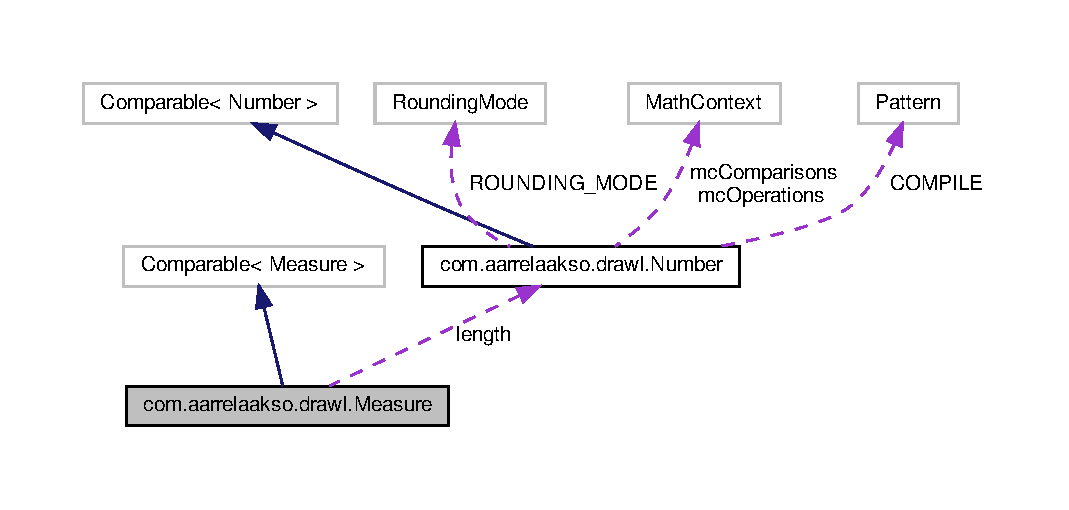
\includegraphics[width=350pt]{d5/ddb/classcom_1_1aarrelaakso_1_1drawl_1_1_measure__coll__graph}
\end{center}
\end{figure}
\subsection*{Public Member Functions}
\begin{DoxyCompactItemize}
\item 
\hyperlink{classcom_1_1aarrelaakso_1_1drawl_1_1_measure_a1eb630b258eb8f181f7e0c96d2df7951}{Measure} (@Not\+Null Integer \hyperlink{classcom_1_1aarrelaakso_1_1drawl_1_1_measure_a13ac55ae968c5e7bed4b3305370d94c5}{length})
\begin{DoxyCompactList}\small\item\em Creates a new \hyperlink{classcom_1_1aarrelaakso_1_1drawl_1_1_measure}{Measure} object from an Integer. \end{DoxyCompactList}\end{DoxyCompactItemize}
\subsection*{Protected Member Functions}
\begin{DoxyCompactItemize}
\item 
\hyperlink{classcom_1_1aarrelaakso_1_1drawl_1_1_measure_a8de66af52cef5213749889357261110b}{Measure} (\hyperlink{classcom_1_1aarrelaakso_1_1drawl_1_1_drawl_number}{Drawl\+Number} \hyperlink{classcom_1_1aarrelaakso_1_1drawl_1_1_measure_a13ac55ae968c5e7bed4b3305370d94c5}{length})
\begin{DoxyCompactList}\small\item\em Creates a new \hyperlink{classcom_1_1aarrelaakso_1_1drawl_1_1_measure}{Measure} object from a \hyperlink{classcom_1_1aarrelaakso_1_1drawl_1_1_drawl_number}{Drawl\+Number}. \end{DoxyCompactList}\item 
\hyperlink{classcom_1_1aarrelaakso_1_1drawl_1_1_drawl_number}{Drawl\+Number} \hyperlink{classcom_1_1aarrelaakso_1_1drawl_1_1_measure_a847bbfcc708d3ff19c89c5303cf69543}{to\+Drawl\+Number} ()
\begin{DoxyCompactList}\small\item\em Converts this \hyperlink{classcom_1_1aarrelaakso_1_1drawl_1_1_measure}{Measure} to a \hyperlink{classcom_1_1aarrelaakso_1_1drawl_1_1_drawl_number}{Drawl\+Number}. \end{DoxyCompactList}\end{DoxyCompactItemize}
\subsection*{Private Attributes}
\begin{DoxyCompactItemize}
\item 
\hyperlink{classcom_1_1aarrelaakso_1_1drawl_1_1_drawl_number}{Drawl\+Number} \hyperlink{classcom_1_1aarrelaakso_1_1drawl_1_1_measure_a13ac55ae968c5e7bed4b3305370d94c5}{length}
\end{DoxyCompactItemize}


\subsection{Detailed Description}
Defines a public \hyperlink{classcom_1_1aarrelaakso_1_1drawl_1_1_measure}{Measure} class to represent measures on the diagram without exposing internal numerical measurements to the user. 

\subsection{Constructor \& Destructor Documentation}
\mbox{\Hypertarget{classcom_1_1aarrelaakso_1_1drawl_1_1_measure_a8de66af52cef5213749889357261110b}\label{classcom_1_1aarrelaakso_1_1drawl_1_1_measure_a8de66af52cef5213749889357261110b}} 
\index{com\+::aarrelaakso\+::drawl\+::\+Measure@{com\+::aarrelaakso\+::drawl\+::\+Measure}!Measure@{Measure}}
\index{Measure@{Measure}!com\+::aarrelaakso\+::drawl\+::\+Measure@{com\+::aarrelaakso\+::drawl\+::\+Measure}}
\subsubsection{\texorpdfstring{Measure()}{Measure()}\hspace{0.1cm}{\footnotesize\ttfamily [1/2]}}
{\footnotesize\ttfamily com.\+aarrelaakso.\+drawl.\+Measure.\+Measure (\begin{DoxyParamCaption}\item[{\hyperlink{classcom_1_1aarrelaakso_1_1drawl_1_1_drawl_number}{Drawl\+Number}}]{length }\end{DoxyParamCaption})\hspace{0.3cm}{\ttfamily [protected]}}



Creates a new \hyperlink{classcom_1_1aarrelaakso_1_1drawl_1_1_measure}{Measure} object from a \hyperlink{classcom_1_1aarrelaakso_1_1drawl_1_1_drawl_number}{Drawl\+Number}. 

In general, this should be the preferred way of constructing a \hyperlink{classcom_1_1aarrelaakso_1_1drawl_1_1_measure}{Measure} object, to keep all underlying math as Drawl\+Numbers, allowing flexibility with the math implementation.


\begin{DoxyParams}{Parameters}
{\em length} & The length to associate with this \hyperlink{classcom_1_1aarrelaakso_1_1drawl_1_1_measure}{Measure}. \\
\hline
\end{DoxyParams}
\mbox{\Hypertarget{classcom_1_1aarrelaakso_1_1drawl_1_1_measure_a1eb630b258eb8f181f7e0c96d2df7951}\label{classcom_1_1aarrelaakso_1_1drawl_1_1_measure_a1eb630b258eb8f181f7e0c96d2df7951}} 
\index{com\+::aarrelaakso\+::drawl\+::\+Measure@{com\+::aarrelaakso\+::drawl\+::\+Measure}!Measure@{Measure}}
\index{Measure@{Measure}!com\+::aarrelaakso\+::drawl\+::\+Measure@{com\+::aarrelaakso\+::drawl\+::\+Measure}}
\subsubsection{\texorpdfstring{Measure()}{Measure()}\hspace{0.1cm}{\footnotesize\ttfamily [2/2]}}
{\footnotesize\ttfamily com.\+aarrelaakso.\+drawl.\+Measure.\+Measure (\begin{DoxyParamCaption}\item[{@Not\+Null Integer}]{length }\end{DoxyParamCaption})}



Creates a new \hyperlink{classcom_1_1aarrelaakso_1_1drawl_1_1_measure}{Measure} object from an Integer. 

Convenience method.


\begin{DoxyParams}{Parameters}
{\em length} & The length to associate with this \hyperlink{classcom_1_1aarrelaakso_1_1drawl_1_1_measure}{Measure}. \\
\hline
\end{DoxyParams}


\subsection{Member Function Documentation}
\mbox{\Hypertarget{classcom_1_1aarrelaakso_1_1drawl_1_1_measure_a847bbfcc708d3ff19c89c5303cf69543}\label{classcom_1_1aarrelaakso_1_1drawl_1_1_measure_a847bbfcc708d3ff19c89c5303cf69543}} 
\index{com\+::aarrelaakso\+::drawl\+::\+Measure@{com\+::aarrelaakso\+::drawl\+::\+Measure}!to\+Drawl\+Number@{to\+Drawl\+Number}}
\index{to\+Drawl\+Number@{to\+Drawl\+Number}!com\+::aarrelaakso\+::drawl\+::\+Measure@{com\+::aarrelaakso\+::drawl\+::\+Measure}}
\subsubsection{\texorpdfstring{to\+Drawl\+Number()}{toDrawlNumber()}}
{\footnotesize\ttfamily \hyperlink{classcom_1_1aarrelaakso_1_1drawl_1_1_drawl_number}{Drawl\+Number} com.\+aarrelaakso.\+drawl.\+Measure.\+to\+Drawl\+Number (\begin{DoxyParamCaption}{ }\end{DoxyParamCaption})\hspace{0.3cm}{\ttfamily [protected]}}



Converts this \hyperlink{classcom_1_1aarrelaakso_1_1drawl_1_1_measure}{Measure} to a \hyperlink{classcom_1_1aarrelaakso_1_1drawl_1_1_drawl_number}{Drawl\+Number}. 

\begin{DoxyReturn}{Returns}
A \hyperlink{classcom_1_1aarrelaakso_1_1drawl_1_1_drawl_number}{Drawl\+Number} representing the length of this Meausre. 
\end{DoxyReturn}


\subsection{Member Data Documentation}
\mbox{\Hypertarget{classcom_1_1aarrelaakso_1_1drawl_1_1_measure_a13ac55ae968c5e7bed4b3305370d94c5}\label{classcom_1_1aarrelaakso_1_1drawl_1_1_measure_a13ac55ae968c5e7bed4b3305370d94c5}} 
\index{com\+::aarrelaakso\+::drawl\+::\+Measure@{com\+::aarrelaakso\+::drawl\+::\+Measure}!length@{length}}
\index{length@{length}!com\+::aarrelaakso\+::drawl\+::\+Measure@{com\+::aarrelaakso\+::drawl\+::\+Measure}}
\subsubsection{\texorpdfstring{length}{length}}
{\footnotesize\ttfamily \hyperlink{classcom_1_1aarrelaakso_1_1drawl_1_1_drawl_number}{Drawl\+Number} com.\+aarrelaakso.\+drawl.\+Measure.\+length\hspace{0.3cm}{\ttfamily [private]}}



The documentation for this class was generated from the following file\+:\begin{DoxyCompactItemize}
\item 
/mnt/d/\+One\+Drive/\+Documents/src/drawl/src/main/java/com/aarrelaakso/drawl/\hyperlink{_measure_8java}{Measure.\+java}\end{DoxyCompactItemize}

\hypertarget{classcom_1_1aarrelaakso_1_1drawl_1_1examples_1_1_nonadjacency}{}\section{com.\+aarrelaakso.\+drawl.\+examples.\+Nonadjacency Class Reference}
\label{classcom_1_1aarrelaakso_1_1drawl_1_1examples_1_1_nonadjacency}\index{com.\+aarrelaakso.\+drawl.\+examples.\+Nonadjacency@{com.\+aarrelaakso.\+drawl.\+examples.\+Nonadjacency}}
\subsection*{Static Public Member Functions}
\begin{DoxyCompactItemize}
\item 
static void \hyperlink{classcom_1_1aarrelaakso_1_1drawl_1_1examples_1_1_nonadjacency_a41d8f11e6e03cf95442b5149f2848183}{main} (String\mbox{[}$\,$\mbox{]} args)  throws I\+O\+Exception     
\end{DoxyCompactItemize}


\subsection{Member Function Documentation}
\mbox{\Hypertarget{classcom_1_1aarrelaakso_1_1drawl_1_1examples_1_1_nonadjacency_a41d8f11e6e03cf95442b5149f2848183}\label{classcom_1_1aarrelaakso_1_1drawl_1_1examples_1_1_nonadjacency_a41d8f11e6e03cf95442b5149f2848183}} 
\index{com\+::aarrelaakso\+::drawl\+::examples\+::\+Nonadjacency@{com\+::aarrelaakso\+::drawl\+::examples\+::\+Nonadjacency}!main@{main}}
\index{main@{main}!com\+::aarrelaakso\+::drawl\+::examples\+::\+Nonadjacency@{com\+::aarrelaakso\+::drawl\+::examples\+::\+Nonadjacency}}
\subsubsection{\texorpdfstring{main()}{main()}}
{\footnotesize\ttfamily static void com.\+aarrelaakso.\+drawl.\+examples.\+Nonadjacency.\+main (\begin{DoxyParamCaption}\item[{String \mbox{[}$\,$\mbox{]}}]{args }\end{DoxyParamCaption}) throws I\+O\+Exception\hspace{0.3cm}{\ttfamily [static]}}



The documentation for this class was generated from the following file\+:\begin{DoxyCompactItemize}
\item 
/mnt/d/\+One\+Drive/\+Documents/src/drawl/src/main/java/com/aarrelaakso/drawl/examples/\hyperlink{_nonadjacency_8java}{Nonadjacency.\+java}\end{DoxyCompactItemize}

\hypertarget{interfacecom_1_1aarrelaakso_1_1drawl_1_1_number}{}\section{com.\+aarrelaakso.\+drawl.\+Number Interface Reference}
\label{interfacecom_1_1aarrelaakso_1_1drawl_1_1_number}\index{com.\+aarrelaakso.\+drawl.\+Number@{com.\+aarrelaakso.\+drawl.\+Number}}


Class for mathematical operations with Double values that have a similar A\+PI to that of the Big\+Decimal class.  




Inheritance diagram for com.\+aarrelaakso.\+drawl.\+Number\+:\nopagebreak
\begin{figure}[H]
\begin{center}
\leavevmode
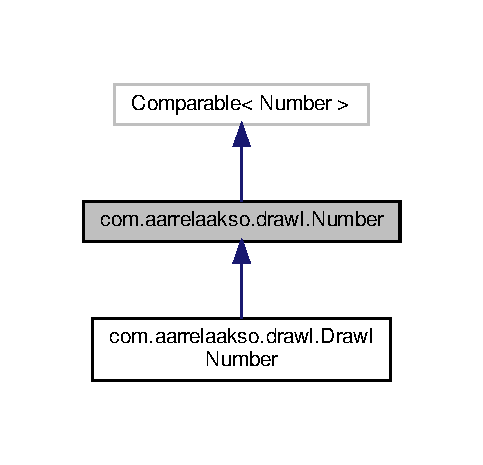
\includegraphics[width=232pt]{d5/de2/interfacecom_1_1aarrelaakso_1_1drawl_1_1_number__inherit__graph}
\end{center}
\end{figure}


Collaboration diagram for com.\+aarrelaakso.\+drawl.\+Number\+:\nopagebreak
\begin{figure}[H]
\begin{center}
\leavevmode
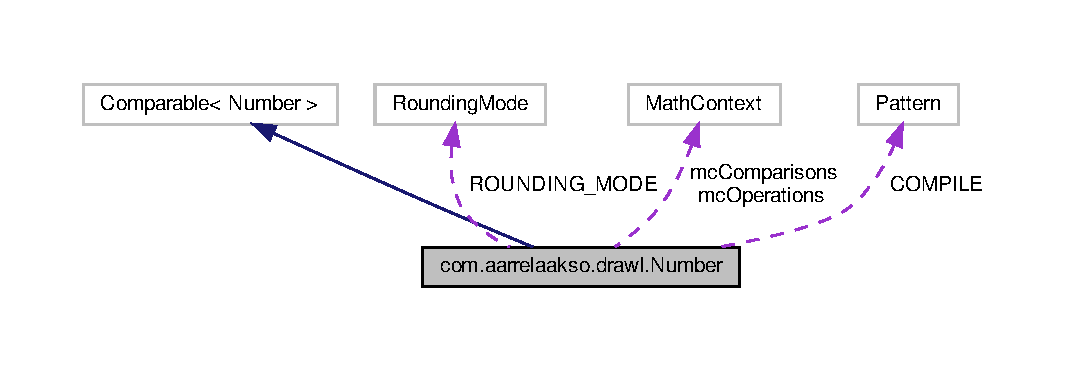
\includegraphics[width=350pt]{df/d78/interfacecom_1_1aarrelaakso_1_1drawl_1_1_number__coll__graph}
\end{center}
\end{figure}
\subsection*{Public Member Functions}
\begin{DoxyCompactItemize}
\item 
boolean \hyperlink{interfacecom_1_1aarrelaakso_1_1drawl_1_1_number_a5bba650d5d9651e83c4ff4364d6f6abc}{is\+Integer\+Value} (@Not\+Null final Big\+Decimal bd)
\begin{DoxyCompactList}\small\item\em Test whether a Big\+Decimal is a mathematical integer. \end{DoxyCompactList}\item 
boolean \hyperlink{interfacecom_1_1aarrelaakso_1_1drawl_1_1_number_a731dbb91dcfd46319662f57c26fcf06a}{is\+Integer\+Value} (final float val)
\begin{DoxyCompactList}\small\item\em Test whether a float is a mathematical integer. \end{DoxyCompactList}\item 
\hyperlink{interfacecom_1_1aarrelaakso_1_1drawl_1_1_number}{Number} \hyperlink{interfacecom_1_1aarrelaakso_1_1drawl_1_1_number_a62af4c1c24c3f9c70dabfe3318e53ac3}{abs} ()
\begin{DoxyCompactList}\small\item\em Returns absolute value of this number. \end{DoxyCompactList}\item 
\hyperlink{interfacecom_1_1aarrelaakso_1_1drawl_1_1_number}{Number} \hyperlink{interfacecom_1_1aarrelaakso_1_1drawl_1_1_number_a05193401712bbba333a586751633c5f6}{add} (@Not\+Null final \hyperlink{interfacecom_1_1aarrelaakso_1_1drawl_1_1_number}{Number} x)
\begin{DoxyCompactList}\small\item\em Performs addition operation. \end{DoxyCompactList}\item 
\hyperlink{interfacecom_1_1aarrelaakso_1_1drawl_1_1_number}{Number} \hyperlink{interfacecom_1_1aarrelaakso_1_1drawl_1_1_number_abd063ef436254888b283a30da6fff78a}{add} (final double x)
\begin{DoxyCompactList}\small\item\em Performs addition operation. \end{DoxyCompactList}\item 
\hyperlink{interfacecom_1_1aarrelaakso_1_1drawl_1_1_number}{Number} \hyperlink{interfacecom_1_1aarrelaakso_1_1drawl_1_1_number_ad71ea7d41bcc751bc6e08ccd0d5f9885}{add} (@Not\+Null final \hyperlink{interfacecom_1_1aarrelaakso_1_1drawl_1_1_number}{Number} augend, final Math\+Context mc)
\begin{DoxyCompactList}\small\item\em Returns a Sisu\+Big\+Decimal whose value is (this + augend), with rounding according to the context settings. \end{DoxyCompactList}\item 
Big\+Decimal \hyperlink{interfacecom_1_1aarrelaakso_1_1drawl_1_1_number_a88d32e8ed7137662dc845ac6937107e6}{big\+Decimal\+Value} ()
\begin{DoxyCompactList}\small\item\em Converts this Sisu\+Big\+Decimal to a Big\+Decimal. \end{DoxyCompactList}\item 
int \hyperlink{interfacecom_1_1aarrelaakso_1_1drawl_1_1_number_a8182808f41dc9573e32884e7155f2776}{compare\+To} (@Not\+Null final \hyperlink{interfacecom_1_1aarrelaakso_1_1drawl_1_1_number}{Number} val)
\begin{DoxyCompactList}\small\item\em Compares this Big\+Decimal with the specified Big\+Decimal. \end{DoxyCompactList}\item 
int \hyperlink{interfacecom_1_1aarrelaakso_1_1drawl_1_1_number_abe6993852fed7bc6f13dbda74b78dde3}{compare\+To\+Fuzzy} (@Not\+Null final \hyperlink{interfacecom_1_1aarrelaakso_1_1drawl_1_1_number}{Number} val)
\begin{DoxyCompactList}\small\item\em Compare this \hyperlink{classcom_1_1aarrelaakso_1_1drawl_1_1_drawl_number}{Drawl\+Number} to another using the default Math\+Context. \end{DoxyCompactList}\item 
int \hyperlink{interfacecom_1_1aarrelaakso_1_1drawl_1_1_number_afb73cae0a12c1d25e450be6270eecfb1}{compare\+To\+Fuzzy} (@Not\+Null final \hyperlink{interfacecom_1_1aarrelaakso_1_1drawl_1_1_number}{Number} val, final Math\+Context mc)
\begin{DoxyCompactList}\small\item\em Compare this \hyperlink{classcom_1_1aarrelaakso_1_1drawl_1_1_drawl_number}{Drawl\+Number} to another fuzzily. \end{DoxyCompactList}\item 
\hyperlink{classcom_1_1aarrelaakso_1_1drawl_1_1_drawl_number_remainder_pair}{Drawl\+Number\+Remainder\+Pair} \hyperlink{interfacecom_1_1aarrelaakso_1_1drawl_1_1_number_abf7f5f2ea47601b2dbf399c68e4bf895}{div\+With\+Remainder} (@Not\+Null final \hyperlink{interfacecom_1_1aarrelaakso_1_1drawl_1_1_number}{Number} x, final int precision)
\begin{DoxyCompactList}\small\item\em Performs division operation and returns the result with remainder. \end{DoxyCompactList}\item 
\hyperlink{classcom_1_1aarrelaakso_1_1drawl_1_1_drawl_number_remainder_pair}{Drawl\+Number\+Remainder\+Pair} \hyperlink{interfacecom_1_1aarrelaakso_1_1drawl_1_1_number_ae3fd76a012e2afc4d71a3ccb93bace92}{div\+With\+Remainder} (final double x, final int precision)
\begin{DoxyCompactList}\small\item\em Performs division operation and returns the result with remainder. \end{DoxyCompactList}\item 
\hyperlink{interfacecom_1_1aarrelaakso_1_1drawl_1_1_number}{Number} \hyperlink{interfacecom_1_1aarrelaakso_1_1drawl_1_1_number_adfd6e1a6e96cbface21eef9b2d8860d0}{divide} (@Not\+Null final \hyperlink{interfacecom_1_1aarrelaakso_1_1drawl_1_1_number}{Number} divisor, final Math\+Context math\+Context)
\begin{DoxyCompactList}\small\item\em Divides with \hyperlink{classcom_1_1aarrelaakso_1_1drawl_1_1_drawl_number}{Drawl\+Number} by another. \end{DoxyCompactList}\item 
\hyperlink{interfacecom_1_1aarrelaakso_1_1drawl_1_1_number}{Number} \hyperlink{interfacecom_1_1aarrelaakso_1_1drawl_1_1_number_acfcd993a82faa41956430086986084e7}{divide} (@Not\+Null final \hyperlink{interfacecom_1_1aarrelaakso_1_1drawl_1_1_number}{Number} divisor, final int precision)
\begin{DoxyCompactList}\small\item\em Divides this \hyperlink{classcom_1_1aarrelaakso_1_1drawl_1_1_drawl_number}{Drawl\+Number} by another. \end{DoxyCompactList}\item 
\hyperlink{interfacecom_1_1aarrelaakso_1_1drawl_1_1_number}{Number} \hyperlink{interfacecom_1_1aarrelaakso_1_1drawl_1_1_number_aa4a70324e7a3dfd7da7fae72cb7fe5b5}{divide} (final double x, final int precision)
\begin{DoxyCompactList}\small\item\em Divides this \hyperlink{classcom_1_1aarrelaakso_1_1drawl_1_1_drawl_number}{Drawl\+Number} by a Double. \end{DoxyCompactList}\item 
double \hyperlink{interfacecom_1_1aarrelaakso_1_1drawl_1_1_number_ad409a636270d5fcc2591791a4e862179}{double\+Value} ()
\begin{DoxyCompactList}\small\item\em Returns double representation of this number. \end{DoxyCompactList}\item 
boolean \hyperlink{interfacecom_1_1aarrelaakso_1_1drawl_1_1_number_afe7ed1040e76bfb7a01c1e3835218827}{equals} (@Not\+Null final \hyperlink{interfacecom_1_1aarrelaakso_1_1drawl_1_1_number}{Number} x)
\begin{DoxyCompactList}\small\item\em Returns whether this number is equal with the other number. \end{DoxyCompactList}\item 
boolean \hyperlink{interfacecom_1_1aarrelaakso_1_1drawl_1_1_number_a102dab4f981a76317b20d69d352ddb15}{equals} (final double x)
\begin{DoxyCompactList}\small\item\em Returns whether this number is equal with the other number. \end{DoxyCompactList}\item 
boolean \hyperlink{interfacecom_1_1aarrelaakso_1_1drawl_1_1_number_a9cf883b0a5979a9f0420cca2c2ff9d89}{equals} (final Object obj)
\begin{DoxyCompactList}\small\item\em Compares this Sisu\+Big\+Decimal with the specified Object for equality. \end{DoxyCompactList}\item 
Float \hyperlink{interfacecom_1_1aarrelaakso_1_1drawl_1_1_number_ad6df5caf5478cc3f85cc808cf39a0610}{float\+Value} ()
\begin{DoxyCompactList}\small\item\em Converts this Big\+Decimal to a Float. \end{DoxyCompactList}\item 
int \hyperlink{interfacecom_1_1aarrelaakso_1_1drawl_1_1_number_a493e402b6856cded24d43022bd1b816a}{hash\+Code} ()
\begin{DoxyCompactList}\small\item\em Returns the hash code for this Sisu\+Big\+Decimal. \end{DoxyCompactList}\item 
Integer \hyperlink{interfacecom_1_1aarrelaakso_1_1drawl_1_1_number_a82bd01108e6f99cba2e83759fa363f39}{int\+Value} ()
\begin{DoxyCompactList}\small\item\em Converts this Big\+Decimal to an Integer. \end{DoxyCompactList}\item 
boolean \hyperlink{interfacecom_1_1aarrelaakso_1_1drawl_1_1_number_aa8ef6fc2e77da054f3a42f2cd81ec8a6}{is\+Equal\+To} (@Not\+Null final \hyperlink{interfacecom_1_1aarrelaakso_1_1drawl_1_1_number}{Number} val)
\begin{DoxyCompactList}\small\item\em Returns whether this number is equal with another number. \end{DoxyCompactList}\item 
boolean \hyperlink{interfacecom_1_1aarrelaakso_1_1drawl_1_1_number_a487be710eb911b7f3395014ee8cd4155}{is\+Greater\+Than} (@Not\+Null final \hyperlink{interfacecom_1_1aarrelaakso_1_1drawl_1_1_number}{Number} val)
\begin{DoxyCompactList}\small\item\em Returns whether this number is greater than the other number. \end{DoxyCompactList}\item 
boolean \hyperlink{interfacecom_1_1aarrelaakso_1_1drawl_1_1_number_ab3c02c742e083e6850ee6d2fe88e985b}{is\+Greater\+Than} (final double val)
\begin{DoxyCompactList}\small\item\em Returns whether this number is greater than the other number. \end{DoxyCompactList}\item 
boolean \hyperlink{interfacecom_1_1aarrelaakso_1_1drawl_1_1_number_a9c3df12a860251807827d670994b89a4}{is\+Greater\+Than\+Or\+Equal\+To} (@Not\+Null final \hyperlink{interfacecom_1_1aarrelaakso_1_1drawl_1_1_number}{Number} val)
\begin{DoxyCompactList}\small\item\em Returns whether this number is greater or equal to the other number. \end{DoxyCompactList}\item 
boolean \hyperlink{interfacecom_1_1aarrelaakso_1_1drawl_1_1_number_ae41d4d8a98ecc4a8e9e3be80d1a6b291}{is\+Greater\+Than\+Or\+Equal\+To} (final double val)
\begin{DoxyCompactList}\small\item\em Returns whether this number is greater or equal to the other number. \end{DoxyCompactList}\item 
boolean \hyperlink{interfacecom_1_1aarrelaakso_1_1drawl_1_1_number_a33d0b6d8f3aeb0ccb9f710739c80f6e7}{is\+Integer\+Value} ()
\begin{DoxyCompactList}\small\item\em Determines whether this \hyperlink{classcom_1_1aarrelaakso_1_1drawl_1_1_drawl_number}{Drawl\+Number} is an integer. \end{DoxyCompactList}\item 
boolean \hyperlink{interfacecom_1_1aarrelaakso_1_1drawl_1_1_number_acc7fec3a209cb27e09a45f17ed9fd4e1}{is\+Less\+Than} (@Not\+Null final \hyperlink{interfacecom_1_1aarrelaakso_1_1drawl_1_1_number}{Number} val)
\begin{DoxyCompactList}\small\item\em Returns whether this number is less than the other number. \end{DoxyCompactList}\item 
boolean \hyperlink{interfacecom_1_1aarrelaakso_1_1drawl_1_1_number_a82b299428c48204fb05229dbea2b439b}{is\+Less\+Than} (final double val)
\begin{DoxyCompactList}\small\item\em Returns whether this number is less than the other number. \end{DoxyCompactList}\item 
boolean \hyperlink{interfacecom_1_1aarrelaakso_1_1drawl_1_1_number_a195d37075fcef873df2907194e794836}{is\+Less\+Than\+Or\+Equal\+To} (@Not\+Null final \hyperlink{interfacecom_1_1aarrelaakso_1_1drawl_1_1_number}{Number} val)
\begin{DoxyCompactList}\small\item\em Returns whether this number is less or equal to the other number. \end{DoxyCompactList}\item 
boolean \hyperlink{interfacecom_1_1aarrelaakso_1_1drawl_1_1_number_a99ddc795a01b241e97345cfd6b85e00b}{is\+Less\+Than\+Or\+Equal\+To} (final double val)
\begin{DoxyCompactList}\small\item\em Returns whether this number is less or equal to the other number. \end{DoxyCompactList}\item 
Boolean \hyperlink{interfacecom_1_1aarrelaakso_1_1drawl_1_1_number_a4684335f60995aca55e4b972fbb3b8ca}{is\+Not\+Equal\+To} (@Not\+Null final \hyperlink{interfacecom_1_1aarrelaakso_1_1drawl_1_1_number}{Number} val)
\begin{DoxyCompactList}\small\item\em Indicates whether another value is not equal to this Sisu\+Big\+Decimal. \end{DoxyCompactList}\item 
\hyperlink{interfacecom_1_1aarrelaakso_1_1drawl_1_1_number}{Number} \hyperlink{interfacecom_1_1aarrelaakso_1_1drawl_1_1_number_a4748fed26ef4d662d7a277dc2687acca}{multiply} (@Not\+Null final \hyperlink{interfacecom_1_1aarrelaakso_1_1drawl_1_1_number}{Number} multiplicand)
\begin{DoxyCompactList}\small\item\em Performs multiplication operation. \end{DoxyCompactList}\item 
\hyperlink{interfacecom_1_1aarrelaakso_1_1drawl_1_1_number}{Number} \hyperlink{interfacecom_1_1aarrelaakso_1_1drawl_1_1_number_a8e43a4a565fb62b7f71a809aa791ecc2}{multiply} (@Not\+Null final \hyperlink{interfacecom_1_1aarrelaakso_1_1drawl_1_1_number}{Number} multiplicand, final Math\+Context mc)
\begin{DoxyCompactList}\small\item\em Returns a Big\+Decimal whose value is (this × multiplicand), with rounding according to the context settings. \end{DoxyCompactList}\item 
\hyperlink{interfacecom_1_1aarrelaakso_1_1drawl_1_1_number}{Number} \hyperlink{interfacecom_1_1aarrelaakso_1_1drawl_1_1_number_a47435944efde1dec963b401dbdf45d62}{multiply} (final double multiplicand)
\begin{DoxyCompactList}\small\item\em Performs multiplication operation. \end{DoxyCompactList}\item 
\hyperlink{interfacecom_1_1aarrelaakso_1_1drawl_1_1_number}{Number} \hyperlink{interfacecom_1_1aarrelaakso_1_1drawl_1_1_number_abeb61241a83c318464f15c0059d65885}{negate} ()
\begin{DoxyCompactList}\small\item\em Negates this number. \end{DoxyCompactList}\item 
\hyperlink{interfacecom_1_1aarrelaakso_1_1drawl_1_1_number}{Number} \hyperlink{interfacecom_1_1aarrelaakso_1_1drawl_1_1_number_a38679e8f0f11db201ee07e3b0541b6a4}{pow} (final int n, final int precision)
\begin{DoxyCompactList}\small\item\em Returns this number powered by n. \end{DoxyCompactList}\item 
\hyperlink{interfacecom_1_1aarrelaakso_1_1drawl_1_1_number}{Number} \hyperlink{interfacecom_1_1aarrelaakso_1_1drawl_1_1_number_aa49b7b3b06a362bdef37241652f35a44}{round} (final Math\+Context mc)
\begin{DoxyCompactList}\small\item\em Create a new instance that has same value as this one rounded. \end{DoxyCompactList}\item 
\hyperlink{interfacecom_1_1aarrelaakso_1_1drawl_1_1_number}{Number} \hyperlink{interfacecom_1_1aarrelaakso_1_1drawl_1_1_number_a0d76b3c8e56e9f18a3ce9baf42be705f}{round} (final int places)
\begin{DoxyCompactList}\small\item\em Create a new instance that has the same value as this one rounded. \end{DoxyCompactList}\item 
\hyperlink{interfacecom_1_1aarrelaakso_1_1drawl_1_1_number}{Number} \hyperlink{interfacecom_1_1aarrelaakso_1_1drawl_1_1_number_ac28e81198ea485a48568a9a543cb5293}{subtract} (@Not\+Null final \hyperlink{interfacecom_1_1aarrelaakso_1_1drawl_1_1_number}{Number} subtrahend)
\begin{DoxyCompactList}\small\item\em Performs subtraction operation. \end{DoxyCompactList}\item 
\hyperlink{interfacecom_1_1aarrelaakso_1_1drawl_1_1_number}{Number} \hyperlink{interfacecom_1_1aarrelaakso_1_1drawl_1_1_number_aae7cf801905b2510138d37ff932c4d30}{subtract} (@Not\+Null final \hyperlink{interfacecom_1_1aarrelaakso_1_1drawl_1_1_number}{Number} subtrahend, final Math\+Context mc)
\begin{DoxyCompactList}\small\item\em Returns a Big\+Decimal whose value is (this -\/ subtrahend), with rounding according to the context settings. \end{DoxyCompactList}\item 
\hyperlink{interfacecom_1_1aarrelaakso_1_1drawl_1_1_number}{Number} \hyperlink{interfacecom_1_1aarrelaakso_1_1drawl_1_1_number_ac04969f656d823c91e55a798df7d6913}{subtract} (final double subtrahend)
\begin{DoxyCompactList}\small\item\em Performs subtraction operation. \end{DoxyCompactList}\item 
String \hyperlink{interfacecom_1_1aarrelaakso_1_1drawl_1_1_number_a8e672210b2f919571e6b09d4cb95c569}{to\+Fixed\+Decimal\+String} (final int num\+Decimals)
\begin{DoxyCompactList}\small\item\em Converts number to the string with fixed decimal digits. \end{DoxyCompactList}\item 
String \hyperlink{interfacecom_1_1aarrelaakso_1_1drawl_1_1_number_accc9efbfff1dfc0ff3d6352e3c1cfd4e}{to\+Full\+String} ()
\begin{DoxyCompactList}\small\item\em Converts this number to the full, containing everything that can be restored. \end{DoxyCompactList}\item 
String \hyperlink{interfacecom_1_1aarrelaakso_1_1drawl_1_1_number_a0c6dd9fbd93fdb6d7e487f507d55ba43}{to\+Plain\+String} ()
\item 
String \hyperlink{interfacecom_1_1aarrelaakso_1_1drawl_1_1_number_a9dc0aea5633aebc8f5888b5a194dcd81}{to\+String} ()
\item 
String \hyperlink{interfacecom_1_1aarrelaakso_1_1drawl_1_1_number_a1cb9c85b621dc2669b2f52a4e82bdd3c}{to\+S\+VG} ()
\begin{DoxyCompactList}\small\item\em Convert this \hyperlink{classcom_1_1aarrelaakso_1_1drawl_1_1_drawl_number}{Drawl\+Number} to a String for \hyperlink{classcom_1_1aarrelaakso_1_1drawl_1_1_s_v_g}{S\+VG}. \end{DoxyCompactList}\end{DoxyCompactItemize}
\subsection*{Public Attributes}
\begin{DoxyCompactItemize}
\item 
Pattern \hyperlink{interfacecom_1_1aarrelaakso_1_1drawl_1_1_number_ad6cff21beec53c9eb5d47ee035e67aa7}{C\+O\+M\+P\+I\+LE} = Pattern.\+compile(\char`\"{}$^\wedge$0+(?!\$)\char`\"{})
\item 
Rounding\+Mode \hyperlink{interfacecom_1_1aarrelaakso_1_1drawl_1_1_number_a98fc7994c62ec7d9a44b11ba2a5b1b02}{R\+O\+U\+N\+D\+I\+N\+G\+\_\+\+M\+O\+DE} = Rounding\+Mode.\+H\+A\+L\+F\+\_\+\+UP
\item 
int \hyperlink{interfacecom_1_1aarrelaakso_1_1drawl_1_1_number_a026ad95b5d9df801218f36987bc1982e}{S\+C\+A\+L\+E\+\_\+\+F\+O\+R\+\_\+\+C\+O\+M\+P\+A\+R\+I\+S\+O\+NS} = 32
\item 
int \hyperlink{interfacecom_1_1aarrelaakso_1_1drawl_1_1_number_afdeba9a614751537318fdb3500ffea79}{S\+C\+A\+L\+E\+\_\+\+F\+O\+R\+\_\+\+O\+P\+E\+R\+A\+T\+I\+O\+NS} = 64
\item 
Math\+Context \hyperlink{interfacecom_1_1aarrelaakso_1_1drawl_1_1_number_ad58946b10553ff37f8b02913de34b664}{mc\+Comparisons} = new Math\+Context(\hyperlink{interfacecom_1_1aarrelaakso_1_1drawl_1_1_number_a026ad95b5d9df801218f36987bc1982e}{S\+C\+A\+L\+E\+\_\+\+F\+O\+R\+\_\+\+C\+O\+M\+P\+A\+R\+I\+S\+O\+NS}, \hyperlink{interfacecom_1_1aarrelaakso_1_1drawl_1_1_number_a98fc7994c62ec7d9a44b11ba2a5b1b02}{R\+O\+U\+N\+D\+I\+N\+G\+\_\+\+M\+O\+DE})
\begin{DoxyCompactList}\small\item\em Use this Math\+Context for comparisons. \end{DoxyCompactList}\item 
Math\+Context \hyperlink{interfacecom_1_1aarrelaakso_1_1drawl_1_1_number_aee829b12bd1d3dc81ecf7bdf4207f778}{mc\+Operations} = new Math\+Context(\hyperlink{interfacecom_1_1aarrelaakso_1_1drawl_1_1_number_afdeba9a614751537318fdb3500ffea79}{S\+C\+A\+L\+E\+\_\+\+F\+O\+R\+\_\+\+O\+P\+E\+R\+A\+T\+I\+O\+NS}, \hyperlink{interfacecom_1_1aarrelaakso_1_1drawl_1_1_number_a98fc7994c62ec7d9a44b11ba2a5b1b02}{R\+O\+U\+N\+D\+I\+N\+G\+\_\+\+M\+O\+DE})
\begin{DoxyCompactList}\small\item\em Use this Math\+Context for other operations, such as multiplying and dividing. \end{DoxyCompactList}\end{DoxyCompactItemize}


\subsection{Detailed Description}
Class for mathematical operations with Double values that have a similar A\+PI to that of the Big\+Decimal class. 

Makes it easier to swap out a Double implementation for a Big\+Decimal implementation (Sisu\+Big\+Decimal) as needs dictate. 

\subsection{Member Function Documentation}
\mbox{\Hypertarget{interfacecom_1_1aarrelaakso_1_1drawl_1_1_number_a62af4c1c24c3f9c70dabfe3318e53ac3}\label{interfacecom_1_1aarrelaakso_1_1drawl_1_1_number_a62af4c1c24c3f9c70dabfe3318e53ac3}} 
\index{com\+::aarrelaakso\+::drawl\+::\+Number@{com\+::aarrelaakso\+::drawl\+::\+Number}!abs@{abs}}
\index{abs@{abs}!com\+::aarrelaakso\+::drawl\+::\+Number@{com\+::aarrelaakso\+::drawl\+::\+Number}}
\subsubsection{\texorpdfstring{abs()}{abs()}}
{\footnotesize\ttfamily \hyperlink{interfacecom_1_1aarrelaakso_1_1drawl_1_1_number}{Number} com.\+aarrelaakso.\+drawl.\+Number.\+abs (\begin{DoxyParamCaption}{ }\end{DoxyParamCaption})}



Returns absolute value of this number. 

\begin{DoxyReturn}{Returns}
absolute value of this number 
\end{DoxyReturn}


Implemented in \hyperlink{classcom_1_1aarrelaakso_1_1drawl_1_1_drawl_number_a2bdcf6f7da129ae45c46f7e91bc65636}{com.\+aarrelaakso.\+drawl.\+Drawl\+Number}.

\mbox{\Hypertarget{interfacecom_1_1aarrelaakso_1_1drawl_1_1_number_a05193401712bbba333a586751633c5f6}\label{interfacecom_1_1aarrelaakso_1_1drawl_1_1_number_a05193401712bbba333a586751633c5f6}} 
\index{com\+::aarrelaakso\+::drawl\+::\+Number@{com\+::aarrelaakso\+::drawl\+::\+Number}!add@{add}}
\index{add@{add}!com\+::aarrelaakso\+::drawl\+::\+Number@{com\+::aarrelaakso\+::drawl\+::\+Number}}
\subsubsection{\texorpdfstring{add()}{add()}\hspace{0.1cm}{\footnotesize\ttfamily [1/3]}}
{\footnotesize\ttfamily \hyperlink{interfacecom_1_1aarrelaakso_1_1drawl_1_1_number}{Number} com.\+aarrelaakso.\+drawl.\+Number.\+add (\begin{DoxyParamCaption}\item[{@Not\+Null final \hyperlink{interfacecom_1_1aarrelaakso_1_1drawl_1_1_number}{Number}}]{x }\end{DoxyParamCaption})}



Performs addition operation. 


\begin{DoxyParams}{Parameters}
{\em x} & other number \\
\hline
\end{DoxyParams}
\begin{DoxyReturn}{Returns}
addition operation result 
\end{DoxyReturn}


Implemented in \hyperlink{classcom_1_1aarrelaakso_1_1drawl_1_1_drawl_number_a484120b1cacb13f1266bf1d3f002ce3d}{com.\+aarrelaakso.\+drawl.\+Drawl\+Number}.

\mbox{\Hypertarget{interfacecom_1_1aarrelaakso_1_1drawl_1_1_number_abd063ef436254888b283a30da6fff78a}\label{interfacecom_1_1aarrelaakso_1_1drawl_1_1_number_abd063ef436254888b283a30da6fff78a}} 
\index{com\+::aarrelaakso\+::drawl\+::\+Number@{com\+::aarrelaakso\+::drawl\+::\+Number}!add@{add}}
\index{add@{add}!com\+::aarrelaakso\+::drawl\+::\+Number@{com\+::aarrelaakso\+::drawl\+::\+Number}}
\subsubsection{\texorpdfstring{add()}{add()}\hspace{0.1cm}{\footnotesize\ttfamily [2/3]}}
{\footnotesize\ttfamily \hyperlink{interfacecom_1_1aarrelaakso_1_1drawl_1_1_number}{Number} com.\+aarrelaakso.\+drawl.\+Number.\+add (\begin{DoxyParamCaption}\item[{final double}]{x }\end{DoxyParamCaption})}



Performs addition operation. 


\begin{DoxyParams}{Parameters}
{\em x} & other number \\
\hline
\end{DoxyParams}
\begin{DoxyReturn}{Returns}
addition operation result 
\end{DoxyReturn}


Implemented in \hyperlink{classcom_1_1aarrelaakso_1_1drawl_1_1_drawl_number_adf7216ecb118a2bbd1d4aba6a51110bc}{com.\+aarrelaakso.\+drawl.\+Drawl\+Number}.

\mbox{\Hypertarget{interfacecom_1_1aarrelaakso_1_1drawl_1_1_number_ad71ea7d41bcc751bc6e08ccd0d5f9885}\label{interfacecom_1_1aarrelaakso_1_1drawl_1_1_number_ad71ea7d41bcc751bc6e08ccd0d5f9885}} 
\index{com\+::aarrelaakso\+::drawl\+::\+Number@{com\+::aarrelaakso\+::drawl\+::\+Number}!add@{add}}
\index{add@{add}!com\+::aarrelaakso\+::drawl\+::\+Number@{com\+::aarrelaakso\+::drawl\+::\+Number}}
\subsubsection{\texorpdfstring{add()}{add()}\hspace{0.1cm}{\footnotesize\ttfamily [3/3]}}
{\footnotesize\ttfamily \hyperlink{interfacecom_1_1aarrelaakso_1_1drawl_1_1_number}{Number} com.\+aarrelaakso.\+drawl.\+Number.\+add (\begin{DoxyParamCaption}\item[{@Not\+Null final \hyperlink{interfacecom_1_1aarrelaakso_1_1drawl_1_1_number}{Number}}]{augend,  }\item[{final Math\+Context}]{mc }\end{DoxyParamCaption})}



Returns a Sisu\+Big\+Decimal whose value is (this + augend), with rounding according to the context settings. 

If either number is zero and the precision setting is nonzero, then the other number, rounded if necessary, is used as the result.


\begin{DoxyParams}{Parameters}
{\em augend} & value to be added to this Sisu\+Big\+Decimal. \\
\hline
{\em mc} & the Math\+Context to use. \\
\hline
\end{DoxyParams}
\begin{DoxyReturn}{Returns}
this + augend, rounded as necessary 
\end{DoxyReturn}


Implemented in \hyperlink{classcom_1_1aarrelaakso_1_1drawl_1_1_drawl_number_a1ecd88ae492b29cf92013f7441f488f8}{com.\+aarrelaakso.\+drawl.\+Drawl\+Number}.

\mbox{\Hypertarget{interfacecom_1_1aarrelaakso_1_1drawl_1_1_number_a88d32e8ed7137662dc845ac6937107e6}\label{interfacecom_1_1aarrelaakso_1_1drawl_1_1_number_a88d32e8ed7137662dc845ac6937107e6}} 
\index{com\+::aarrelaakso\+::drawl\+::\+Number@{com\+::aarrelaakso\+::drawl\+::\+Number}!big\+Decimal\+Value@{big\+Decimal\+Value}}
\index{big\+Decimal\+Value@{big\+Decimal\+Value}!com\+::aarrelaakso\+::drawl\+::\+Number@{com\+::aarrelaakso\+::drawl\+::\+Number}}
\subsubsection{\texorpdfstring{big\+Decimal\+Value()}{bigDecimalValue()}}
{\footnotesize\ttfamily Big\+Decimal com.\+aarrelaakso.\+drawl.\+Number.\+big\+Decimal\+Value (\begin{DoxyParamCaption}{ }\end{DoxyParamCaption})}



Converts this Sisu\+Big\+Decimal to a Big\+Decimal. 

\begin{DoxyReturn}{Returns}
this Sisu\+Big\+Decimal converted to a Big\+Decimal. 
\end{DoxyReturn}


Implemented in \hyperlink{classcom_1_1aarrelaakso_1_1drawl_1_1_drawl_number_acf97abc572acd173a4d8cd6c5b5c2ecd}{com.\+aarrelaakso.\+drawl.\+Drawl\+Number}.

\mbox{\Hypertarget{interfacecom_1_1aarrelaakso_1_1drawl_1_1_number_a8182808f41dc9573e32884e7155f2776}\label{interfacecom_1_1aarrelaakso_1_1drawl_1_1_number_a8182808f41dc9573e32884e7155f2776}} 
\index{com\+::aarrelaakso\+::drawl\+::\+Number@{com\+::aarrelaakso\+::drawl\+::\+Number}!compare\+To@{compare\+To}}
\index{compare\+To@{compare\+To}!com\+::aarrelaakso\+::drawl\+::\+Number@{com\+::aarrelaakso\+::drawl\+::\+Number}}
\subsubsection{\texorpdfstring{compare\+To()}{compareTo()}}
{\footnotesize\ttfamily int com.\+aarrelaakso.\+drawl.\+Number.\+compare\+To (\begin{DoxyParamCaption}\item[{@Not\+Null final \hyperlink{interfacecom_1_1aarrelaakso_1_1drawl_1_1_number}{Number}}]{val }\end{DoxyParamCaption})}



Compares this Big\+Decimal with the specified Big\+Decimal. 

Two Big\+Decimal objects that are equal in value but have a different scale (like 2.\+0 and 2.\+00) are considered equal by this method. 

This method overrides the compare\+To method in the java.\+lang.\+Comparable interface.


\begin{DoxyParams}{Parameters}
{\em val} & Big\+Decimal to which this Big\+Decimal is to be compared. \\
\hline
\end{DoxyParams}
\begin{DoxyReturn}{Returns}
-\/1, 0, or 1 as this Big\+Decimal is numerically less than, equal to, or greater than val. 
\end{DoxyReturn}


Implemented in \hyperlink{classcom_1_1aarrelaakso_1_1drawl_1_1_drawl_number_a40d2c6535f85306aaf5b6e5886c51266}{com.\+aarrelaakso.\+drawl.\+Drawl\+Number}.

\mbox{\Hypertarget{interfacecom_1_1aarrelaakso_1_1drawl_1_1_number_abe6993852fed7bc6f13dbda74b78dde3}\label{interfacecom_1_1aarrelaakso_1_1drawl_1_1_number_abe6993852fed7bc6f13dbda74b78dde3}} 
\index{com\+::aarrelaakso\+::drawl\+::\+Number@{com\+::aarrelaakso\+::drawl\+::\+Number}!compare\+To\+Fuzzy@{compare\+To\+Fuzzy}}
\index{compare\+To\+Fuzzy@{compare\+To\+Fuzzy}!com\+::aarrelaakso\+::drawl\+::\+Number@{com\+::aarrelaakso\+::drawl\+::\+Number}}
\subsubsection{\texorpdfstring{compare\+To\+Fuzzy()}{compareToFuzzy()}\hspace{0.1cm}{\footnotesize\ttfamily [1/2]}}
{\footnotesize\ttfamily int com.\+aarrelaakso.\+drawl.\+Number.\+compare\+To\+Fuzzy (\begin{DoxyParamCaption}\item[{@Not\+Null final \hyperlink{interfacecom_1_1aarrelaakso_1_1drawl_1_1_number}{Number}}]{val }\end{DoxyParamCaption})}



Compare this \hyperlink{classcom_1_1aarrelaakso_1_1drawl_1_1_drawl_number}{Drawl\+Number} to another using the default Math\+Context. 


\begin{DoxyParams}{Parameters}
{\em val} & The other \hyperlink{classcom_1_1aarrelaakso_1_1drawl_1_1_drawl_number}{Drawl\+Number} to compare to this one. \\
\hline
\end{DoxyParams}
\begin{DoxyReturn}{Returns}
-\/1, 0, or 1 as this Big\+Decimal is numerically less than, equal to, or greater than val. 
\end{DoxyReturn}


Implemented in \hyperlink{classcom_1_1aarrelaakso_1_1drawl_1_1_drawl_number_ab2624aa98592bb5dd20990c7f5921024}{com.\+aarrelaakso.\+drawl.\+Drawl\+Number}.

\mbox{\Hypertarget{interfacecom_1_1aarrelaakso_1_1drawl_1_1_number_afb73cae0a12c1d25e450be6270eecfb1}\label{interfacecom_1_1aarrelaakso_1_1drawl_1_1_number_afb73cae0a12c1d25e450be6270eecfb1}} 
\index{com\+::aarrelaakso\+::drawl\+::\+Number@{com\+::aarrelaakso\+::drawl\+::\+Number}!compare\+To\+Fuzzy@{compare\+To\+Fuzzy}}
\index{compare\+To\+Fuzzy@{compare\+To\+Fuzzy}!com\+::aarrelaakso\+::drawl\+::\+Number@{com\+::aarrelaakso\+::drawl\+::\+Number}}
\subsubsection{\texorpdfstring{compare\+To\+Fuzzy()}{compareToFuzzy()}\hspace{0.1cm}{\footnotesize\ttfamily [2/2]}}
{\footnotesize\ttfamily int com.\+aarrelaakso.\+drawl.\+Number.\+compare\+To\+Fuzzy (\begin{DoxyParamCaption}\item[{@Not\+Null final \hyperlink{interfacecom_1_1aarrelaakso_1_1drawl_1_1_number}{Number}}]{val,  }\item[{final Math\+Context}]{mc }\end{DoxyParamCaption})}



Compare this \hyperlink{classcom_1_1aarrelaakso_1_1drawl_1_1_drawl_number}{Drawl\+Number} to another fuzzily. 


\begin{DoxyParams}{Parameters}
{\em val} & The other \hyperlink{classcom_1_1aarrelaakso_1_1drawl_1_1_drawl_number}{Drawl\+Number} to compare to this one. \\
\hline
{\em mc} & A Math\+Context object. The precision field (total number of significant digits) is used as the scale (number of digits to the right of the decimal place) for this operation. \\
\hline
\end{DoxyParams}
\begin{DoxyReturn}{Returns}
-\/1, 0, or 1 as this Big\+Decimal is numerically less than, equal to, or greater than val. 
\end{DoxyReturn}


Implemented in \hyperlink{classcom_1_1aarrelaakso_1_1drawl_1_1_drawl_number_a67bb221c313ba22d920db646d130d66f}{com.\+aarrelaakso.\+drawl.\+Drawl\+Number}.

\mbox{\Hypertarget{interfacecom_1_1aarrelaakso_1_1drawl_1_1_number_adfd6e1a6e96cbface21eef9b2d8860d0}\label{interfacecom_1_1aarrelaakso_1_1drawl_1_1_number_adfd6e1a6e96cbface21eef9b2d8860d0}} 
\index{com\+::aarrelaakso\+::drawl\+::\+Number@{com\+::aarrelaakso\+::drawl\+::\+Number}!divide@{divide}}
\index{divide@{divide}!com\+::aarrelaakso\+::drawl\+::\+Number@{com\+::aarrelaakso\+::drawl\+::\+Number}}
\subsubsection{\texorpdfstring{divide()}{divide()}\hspace{0.1cm}{\footnotesize\ttfamily [1/3]}}
{\footnotesize\ttfamily \hyperlink{interfacecom_1_1aarrelaakso_1_1drawl_1_1_number}{Number} com.\+aarrelaakso.\+drawl.\+Number.\+divide (\begin{DoxyParamCaption}\item[{@Not\+Null final \hyperlink{interfacecom_1_1aarrelaakso_1_1drawl_1_1_number}{Number}}]{divisor,  }\item[{final Math\+Context}]{math\+Context }\end{DoxyParamCaption})}



Divides with \hyperlink{classcom_1_1aarrelaakso_1_1drawl_1_1_drawl_number}{Drawl\+Number} by another. 


\begin{DoxyParams}{Parameters}
{\em divisor} & The divisor. \\
\hline
{\em math\+Context} & Ignored. Retained for compatibility with \hyperlink{classcom_1_1aarrelaakso_1_1drawl_1_1_sisu_number}{Sisu\+Number} interface. \\
\hline
\end{DoxyParams}
\begin{DoxyReturn}{Returns}
This divided by val. 
\end{DoxyReturn}


Implemented in \hyperlink{classcom_1_1aarrelaakso_1_1drawl_1_1_drawl_number_ad6350a9965757a1ffeb859d71ee0219e}{com.\+aarrelaakso.\+drawl.\+Drawl\+Number}.

\mbox{\Hypertarget{interfacecom_1_1aarrelaakso_1_1drawl_1_1_number_acfcd993a82faa41956430086986084e7}\label{interfacecom_1_1aarrelaakso_1_1drawl_1_1_number_acfcd993a82faa41956430086986084e7}} 
\index{com\+::aarrelaakso\+::drawl\+::\+Number@{com\+::aarrelaakso\+::drawl\+::\+Number}!divide@{divide}}
\index{divide@{divide}!com\+::aarrelaakso\+::drawl\+::\+Number@{com\+::aarrelaakso\+::drawl\+::\+Number}}
\subsubsection{\texorpdfstring{divide()}{divide()}\hspace{0.1cm}{\footnotesize\ttfamily [2/3]}}
{\footnotesize\ttfamily \hyperlink{interfacecom_1_1aarrelaakso_1_1drawl_1_1_number}{Number} com.\+aarrelaakso.\+drawl.\+Number.\+divide (\begin{DoxyParamCaption}\item[{@Not\+Null final \hyperlink{interfacecom_1_1aarrelaakso_1_1drawl_1_1_number}{Number}}]{divisor,  }\item[{final int}]{precision }\end{DoxyParamCaption})}



Divides this \hyperlink{classcom_1_1aarrelaakso_1_1drawl_1_1_drawl_number}{Drawl\+Number} by another. 


\begin{DoxyParams}{Parameters}
{\em divisor} & divisor number \\
\hline
{\em precision} & The precision (number of significant digits) of the result. \\
\hline
\end{DoxyParams}
\begin{DoxyReturn}{Returns}
division operation result 
\end{DoxyReturn}


Implemented in \hyperlink{classcom_1_1aarrelaakso_1_1drawl_1_1_drawl_number_a24ee9901f4d84a2fc086d4e727bf40c7}{com.\+aarrelaakso.\+drawl.\+Drawl\+Number}.

\mbox{\Hypertarget{interfacecom_1_1aarrelaakso_1_1drawl_1_1_number_aa4a70324e7a3dfd7da7fae72cb7fe5b5}\label{interfacecom_1_1aarrelaakso_1_1drawl_1_1_number_aa4a70324e7a3dfd7da7fae72cb7fe5b5}} 
\index{com\+::aarrelaakso\+::drawl\+::\+Number@{com\+::aarrelaakso\+::drawl\+::\+Number}!divide@{divide}}
\index{divide@{divide}!com\+::aarrelaakso\+::drawl\+::\+Number@{com\+::aarrelaakso\+::drawl\+::\+Number}}
\subsubsection{\texorpdfstring{divide()}{divide()}\hspace{0.1cm}{\footnotesize\ttfamily [3/3]}}
{\footnotesize\ttfamily \hyperlink{interfacecom_1_1aarrelaakso_1_1drawl_1_1_number}{Number} com.\+aarrelaakso.\+drawl.\+Number.\+divide (\begin{DoxyParamCaption}\item[{final double}]{x,  }\item[{final int}]{precision }\end{DoxyParamCaption})}



Divides this \hyperlink{classcom_1_1aarrelaakso_1_1drawl_1_1_drawl_number}{Drawl\+Number} by a Double. 


\begin{DoxyParams}{Parameters}
{\em x} & divisor number \\
\hline
{\em precision} & precision of the result (see the class level comment for details) \\
\hline
\end{DoxyParams}
\begin{DoxyReturn}{Returns}
division operation result 
\end{DoxyReturn}


Implemented in \hyperlink{classcom_1_1aarrelaakso_1_1drawl_1_1_drawl_number_a4ba0f1728e95fe494d440c04228041f7}{com.\+aarrelaakso.\+drawl.\+Drawl\+Number}.

\mbox{\Hypertarget{interfacecom_1_1aarrelaakso_1_1drawl_1_1_number_abf7f5f2ea47601b2dbf399c68e4bf895}\label{interfacecom_1_1aarrelaakso_1_1drawl_1_1_number_abf7f5f2ea47601b2dbf399c68e4bf895}} 
\index{com\+::aarrelaakso\+::drawl\+::\+Number@{com\+::aarrelaakso\+::drawl\+::\+Number}!div\+With\+Remainder@{div\+With\+Remainder}}
\index{div\+With\+Remainder@{div\+With\+Remainder}!com\+::aarrelaakso\+::drawl\+::\+Number@{com\+::aarrelaakso\+::drawl\+::\+Number}}
\subsubsection{\texorpdfstring{div\+With\+Remainder()}{divWithRemainder()}\hspace{0.1cm}{\footnotesize\ttfamily [1/2]}}
{\footnotesize\ttfamily \hyperlink{classcom_1_1aarrelaakso_1_1drawl_1_1_drawl_number_remainder_pair}{Drawl\+Number\+Remainder\+Pair} com.\+aarrelaakso.\+drawl.\+Number.\+div\+With\+Remainder (\begin{DoxyParamCaption}\item[{@Not\+Null final \hyperlink{interfacecom_1_1aarrelaakso_1_1drawl_1_1_number}{Number}}]{x,  }\item[{final int}]{precision }\end{DoxyParamCaption})}



Performs division operation and returns the result with remainder. 


\begin{DoxyParams}{Parameters}
{\em x} & divisor number \\
\hline
{\em precision} & This parameter is ignored. It is preserved for interface compatibility with Sisu\+Big\+Decimal. \\
\hline
\end{DoxyParams}
\begin{DoxyReturn}{Returns}
division operation result 
\end{DoxyReturn}


Implemented in \hyperlink{classcom_1_1aarrelaakso_1_1drawl_1_1_drawl_number_a452c8b23180fe298592093adde0fa87e}{com.\+aarrelaakso.\+drawl.\+Drawl\+Number}.

\mbox{\Hypertarget{interfacecom_1_1aarrelaakso_1_1drawl_1_1_number_ae3fd76a012e2afc4d71a3ccb93bace92}\label{interfacecom_1_1aarrelaakso_1_1drawl_1_1_number_ae3fd76a012e2afc4d71a3ccb93bace92}} 
\index{com\+::aarrelaakso\+::drawl\+::\+Number@{com\+::aarrelaakso\+::drawl\+::\+Number}!div\+With\+Remainder@{div\+With\+Remainder}}
\index{div\+With\+Remainder@{div\+With\+Remainder}!com\+::aarrelaakso\+::drawl\+::\+Number@{com\+::aarrelaakso\+::drawl\+::\+Number}}
\subsubsection{\texorpdfstring{div\+With\+Remainder()}{divWithRemainder()}\hspace{0.1cm}{\footnotesize\ttfamily [2/2]}}
{\footnotesize\ttfamily \hyperlink{classcom_1_1aarrelaakso_1_1drawl_1_1_drawl_number_remainder_pair}{Drawl\+Number\+Remainder\+Pair} com.\+aarrelaakso.\+drawl.\+Number.\+div\+With\+Remainder (\begin{DoxyParamCaption}\item[{final double}]{x,  }\item[{final int}]{precision }\end{DoxyParamCaption})}



Performs division operation and returns the result with remainder. 


\begin{DoxyParams}{Parameters}
{\em x} & divisor number \\
\hline
{\em precision} & precision of the result (see the class level comment for details) \\
\hline
\end{DoxyParams}
\begin{DoxyReturn}{Returns}
division operation result 
\end{DoxyReturn}


Implemented in \hyperlink{classcom_1_1aarrelaakso_1_1drawl_1_1_drawl_number_a6dc7cefb2574b9675ab3bc099760cbd2}{com.\+aarrelaakso.\+drawl.\+Drawl\+Number}.

\mbox{\Hypertarget{interfacecom_1_1aarrelaakso_1_1drawl_1_1_number_ad409a636270d5fcc2591791a4e862179}\label{interfacecom_1_1aarrelaakso_1_1drawl_1_1_number_ad409a636270d5fcc2591791a4e862179}} 
\index{com\+::aarrelaakso\+::drawl\+::\+Number@{com\+::aarrelaakso\+::drawl\+::\+Number}!double\+Value@{double\+Value}}
\index{double\+Value@{double\+Value}!com\+::aarrelaakso\+::drawl\+::\+Number@{com\+::aarrelaakso\+::drawl\+::\+Number}}
\subsubsection{\texorpdfstring{double\+Value()}{doubleValue()}}
{\footnotesize\ttfamily double com.\+aarrelaakso.\+drawl.\+Number.\+double\+Value (\begin{DoxyParamCaption}{ }\end{DoxyParamCaption})}



Returns double representation of this number. 

Conversion might ended up by loosing the precision.

\begin{DoxyReturn}{Returns}
double representation of this value 
\end{DoxyReturn}


Implemented in \hyperlink{classcom_1_1aarrelaakso_1_1drawl_1_1_drawl_number_af5e6d77e51e7b6167d18acec2eb26877}{com.\+aarrelaakso.\+drawl.\+Drawl\+Number}.

\mbox{\Hypertarget{interfacecom_1_1aarrelaakso_1_1drawl_1_1_number_afe7ed1040e76bfb7a01c1e3835218827}\label{interfacecom_1_1aarrelaakso_1_1drawl_1_1_number_afe7ed1040e76bfb7a01c1e3835218827}} 
\index{com\+::aarrelaakso\+::drawl\+::\+Number@{com\+::aarrelaakso\+::drawl\+::\+Number}!equals@{equals}}
\index{equals@{equals}!com\+::aarrelaakso\+::drawl\+::\+Number@{com\+::aarrelaakso\+::drawl\+::\+Number}}
\subsubsection{\texorpdfstring{equals()}{equals()}\hspace{0.1cm}{\footnotesize\ttfamily [1/3]}}
{\footnotesize\ttfamily boolean com.\+aarrelaakso.\+drawl.\+Number.\+equals (\begin{DoxyParamCaption}\item[{@Not\+Null final \hyperlink{interfacecom_1_1aarrelaakso_1_1drawl_1_1_number}{Number}}]{x }\end{DoxyParamCaption})}



Returns whether this number is equal with the other number. 


\begin{DoxyParams}{Parameters}
{\em x} & tested number \\
\hline
\end{DoxyParams}
\begin{DoxyReturn}{Returns}
true if this number is equal to the other number 
\end{DoxyReturn}


Implemented in \hyperlink{classcom_1_1aarrelaakso_1_1drawl_1_1_drawl_number_ad5b1c1aea2f1d2d04a9064a3041059c5}{com.\+aarrelaakso.\+drawl.\+Drawl\+Number}.

\mbox{\Hypertarget{interfacecom_1_1aarrelaakso_1_1drawl_1_1_number_a102dab4f981a76317b20d69d352ddb15}\label{interfacecom_1_1aarrelaakso_1_1drawl_1_1_number_a102dab4f981a76317b20d69d352ddb15}} 
\index{com\+::aarrelaakso\+::drawl\+::\+Number@{com\+::aarrelaakso\+::drawl\+::\+Number}!equals@{equals}}
\index{equals@{equals}!com\+::aarrelaakso\+::drawl\+::\+Number@{com\+::aarrelaakso\+::drawl\+::\+Number}}
\subsubsection{\texorpdfstring{equals()}{equals()}\hspace{0.1cm}{\footnotesize\ttfamily [2/3]}}
{\footnotesize\ttfamily boolean com.\+aarrelaakso.\+drawl.\+Number.\+equals (\begin{DoxyParamCaption}\item[{final double}]{x }\end{DoxyParamCaption})}



Returns whether this number is equal with the other number. 


\begin{DoxyParams}{Parameters}
{\em x} & tested number \\
\hline
\end{DoxyParams}
\begin{DoxyReturn}{Returns}
true if this number is equal to the other number 
\end{DoxyReturn}


Implemented in \hyperlink{classcom_1_1aarrelaakso_1_1drawl_1_1_drawl_number_a09dfa96894d84cc9734e41bf4a88ae3b}{com.\+aarrelaakso.\+drawl.\+Drawl\+Number}.

\mbox{\Hypertarget{interfacecom_1_1aarrelaakso_1_1drawl_1_1_number_a9cf883b0a5979a9f0420cca2c2ff9d89}\label{interfacecom_1_1aarrelaakso_1_1drawl_1_1_number_a9cf883b0a5979a9f0420cca2c2ff9d89}} 
\index{com\+::aarrelaakso\+::drawl\+::\+Number@{com\+::aarrelaakso\+::drawl\+::\+Number}!equals@{equals}}
\index{equals@{equals}!com\+::aarrelaakso\+::drawl\+::\+Number@{com\+::aarrelaakso\+::drawl\+::\+Number}}
\subsubsection{\texorpdfstring{equals()}{equals()}\hspace{0.1cm}{\footnotesize\ttfamily [3/3]}}
{\footnotesize\ttfamily boolean com.\+aarrelaakso.\+drawl.\+Number.\+equals (\begin{DoxyParamCaption}\item[{final Object}]{obj }\end{DoxyParamCaption})}



Compares this Sisu\+Big\+Decimal with the specified Object for equality. 

Unlike compare\+To, this method considers two Sisu\+Big\+Decimal objects equal only if they are equal in value and scale (thus 2.\+0 is not equal to 2.\+00 when compared by this method).


\begin{DoxyParams}{Parameters}
{\em obj} & Object to which this Big\+Decimal is to be compared. \\
\hline
\end{DoxyParams}
\begin{DoxyReturn}{Returns}
true if and only if the specified Object is a Sisu\+Big\+Decimal whose value and scale are equal to this Sisu\+Big\+Decimal\textquotesingle{}s. 
\end{DoxyReturn}


Implemented in \hyperlink{classcom_1_1aarrelaakso_1_1drawl_1_1_drawl_number_a54d65831347b02b14569ddfc021a4ade}{com.\+aarrelaakso.\+drawl.\+Drawl\+Number}.

\mbox{\Hypertarget{interfacecom_1_1aarrelaakso_1_1drawl_1_1_number_ad6df5caf5478cc3f85cc808cf39a0610}\label{interfacecom_1_1aarrelaakso_1_1drawl_1_1_number_ad6df5caf5478cc3f85cc808cf39a0610}} 
\index{com\+::aarrelaakso\+::drawl\+::\+Number@{com\+::aarrelaakso\+::drawl\+::\+Number}!float\+Value@{float\+Value}}
\index{float\+Value@{float\+Value}!com\+::aarrelaakso\+::drawl\+::\+Number@{com\+::aarrelaakso\+::drawl\+::\+Number}}
\subsubsection{\texorpdfstring{float\+Value()}{floatValue()}}
{\footnotesize\ttfamily Float com.\+aarrelaakso.\+drawl.\+Number.\+float\+Value (\begin{DoxyParamCaption}{ }\end{DoxyParamCaption})}



Converts this Big\+Decimal to a Float. 

This conversion is similar to the narrowing primitive conversion from double to float as defined in section 5.\+1.\+3 of The Java™ Language Specification\+: if this Big\+Decimal has too great a magnitude to represent as a Float, it will be converted to Float.\+N\+E\+G\+A\+T\+I\+V\+E\+\_\+\+I\+N\+F\+I\+N\+I\+TY or Float.\+P\+O\+S\+I\+T\+I\+V\+E\+\_\+\+I\+N\+F\+I\+N\+I\+TY as appropriate. Note that even when the return value is finite, this conversion can lose information about the precision of the Big\+Decimal value.

\begin{DoxyReturn}{Returns}
this Sisu\+Big\+Decimal converted to a Float. 
\end{DoxyReturn}


Implemented in \hyperlink{classcom_1_1aarrelaakso_1_1drawl_1_1_drawl_number_ae8442cbd5cc7ab0c35c0302b196b3819}{com.\+aarrelaakso.\+drawl.\+Drawl\+Number}.

\mbox{\Hypertarget{interfacecom_1_1aarrelaakso_1_1drawl_1_1_number_a493e402b6856cded24d43022bd1b816a}\label{interfacecom_1_1aarrelaakso_1_1drawl_1_1_number_a493e402b6856cded24d43022bd1b816a}} 
\index{com\+::aarrelaakso\+::drawl\+::\+Number@{com\+::aarrelaakso\+::drawl\+::\+Number}!hash\+Code@{hash\+Code}}
\index{hash\+Code@{hash\+Code}!com\+::aarrelaakso\+::drawl\+::\+Number@{com\+::aarrelaakso\+::drawl\+::\+Number}}
\subsubsection{\texorpdfstring{hash\+Code()}{hashCode()}}
{\footnotesize\ttfamily int com.\+aarrelaakso.\+drawl.\+Number.\+hash\+Code (\begin{DoxyParamCaption}{ }\end{DoxyParamCaption})}



Returns the hash code for this Sisu\+Big\+Decimal. 

Note that two Sisu\+Big\+Decimal objects that are numerically equal but differ in scale (like 2.\+0 and 2.\+00) will generally not have the same hash code.

\begin{DoxyReturn}{Returns}
hash code for this Big\+Decimal. 
\end{DoxyReturn}


Implemented in \hyperlink{classcom_1_1aarrelaakso_1_1drawl_1_1_drawl_number_a0048361007923e4b902a4581eb9ba45c}{com.\+aarrelaakso.\+drawl.\+Drawl\+Number}.

\mbox{\Hypertarget{interfacecom_1_1aarrelaakso_1_1drawl_1_1_number_a82bd01108e6f99cba2e83759fa363f39}\label{interfacecom_1_1aarrelaakso_1_1drawl_1_1_number_a82bd01108e6f99cba2e83759fa363f39}} 
\index{com\+::aarrelaakso\+::drawl\+::\+Number@{com\+::aarrelaakso\+::drawl\+::\+Number}!int\+Value@{int\+Value}}
\index{int\+Value@{int\+Value}!com\+::aarrelaakso\+::drawl\+::\+Number@{com\+::aarrelaakso\+::drawl\+::\+Number}}
\subsubsection{\texorpdfstring{int\+Value()}{intValue()}}
{\footnotesize\ttfamily Integer com.\+aarrelaakso.\+drawl.\+Number.\+int\+Value (\begin{DoxyParamCaption}{ }\end{DoxyParamCaption})}



Converts this Big\+Decimal to an Integer. 

This conversion is analogous to the narrowing primitive conversion from double to short as defined in section 5.\+1.\+3 of The Java™ Language Specification\+: any fractional part of this Big\+Decimal will be discarded, and if the resulting \char`\"{}\+Big\+Integer\char`\"{} is too big to fit in an int, only the low-\/order 32 bits are returned. Note that this conversion can lose information about the overall magnitude and precision of this Big\+Decimal value as well as return a result with the opposite sign.

\begin{DoxyReturn}{Returns}
this Big\+Decimal converted to an Integer. 
\end{DoxyReturn}


Implemented in \hyperlink{classcom_1_1aarrelaakso_1_1drawl_1_1_drawl_number_a8022d04415c5449344ac1e23658f8802}{com.\+aarrelaakso.\+drawl.\+Drawl\+Number}.

\mbox{\Hypertarget{interfacecom_1_1aarrelaakso_1_1drawl_1_1_number_aa8ef6fc2e77da054f3a42f2cd81ec8a6}\label{interfacecom_1_1aarrelaakso_1_1drawl_1_1_number_aa8ef6fc2e77da054f3a42f2cd81ec8a6}} 
\index{com\+::aarrelaakso\+::drawl\+::\+Number@{com\+::aarrelaakso\+::drawl\+::\+Number}!is\+Equal\+To@{is\+Equal\+To}}
\index{is\+Equal\+To@{is\+Equal\+To}!com\+::aarrelaakso\+::drawl\+::\+Number@{com\+::aarrelaakso\+::drawl\+::\+Number}}
\subsubsection{\texorpdfstring{is\+Equal\+To()}{isEqualTo()}}
{\footnotesize\ttfamily boolean com.\+aarrelaakso.\+drawl.\+Number.\+is\+Equal\+To (\begin{DoxyParamCaption}\item[{@Not\+Null final \hyperlink{interfacecom_1_1aarrelaakso_1_1drawl_1_1_number}{Number}}]{val }\end{DoxyParamCaption})}



Returns whether this number is equal with another number. 


\begin{DoxyParams}{Parameters}
{\em val} & tested number \\
\hline
\end{DoxyParams}
\begin{DoxyReturn}{Returns}
true if this number is equal to the other number 
\end{DoxyReturn}
\begin{DoxyAuthor}{Author}
Aarre Laakso 
\end{DoxyAuthor}
\begin{DoxyVersion}{Version}
1.\+0, 04/28/2020 
\end{DoxyVersion}
\begin{DoxySince}{Since}
04/28/2020 
\end{DoxySince}


Implemented in \hyperlink{classcom_1_1aarrelaakso_1_1drawl_1_1_drawl_number_af9c62a136858a5eae279039658a2cfdc}{com.\+aarrelaakso.\+drawl.\+Drawl\+Number}.

\mbox{\Hypertarget{interfacecom_1_1aarrelaakso_1_1drawl_1_1_number_a487be710eb911b7f3395014ee8cd4155}\label{interfacecom_1_1aarrelaakso_1_1drawl_1_1_number_a487be710eb911b7f3395014ee8cd4155}} 
\index{com\+::aarrelaakso\+::drawl\+::\+Number@{com\+::aarrelaakso\+::drawl\+::\+Number}!is\+Greater\+Than@{is\+Greater\+Than}}
\index{is\+Greater\+Than@{is\+Greater\+Than}!com\+::aarrelaakso\+::drawl\+::\+Number@{com\+::aarrelaakso\+::drawl\+::\+Number}}
\subsubsection{\texorpdfstring{is\+Greater\+Than()}{isGreaterThan()}\hspace{0.1cm}{\footnotesize\ttfamily [1/2]}}
{\footnotesize\ttfamily boolean com.\+aarrelaakso.\+drawl.\+Number.\+is\+Greater\+Than (\begin{DoxyParamCaption}\item[{@Not\+Null final \hyperlink{interfacecom_1_1aarrelaakso_1_1drawl_1_1_number}{Number}}]{val }\end{DoxyParamCaption})}



Returns whether this number is greater than the other number. 


\begin{DoxyParams}{Parameters}
{\em val} & tested number \\
\hline
\end{DoxyParams}
\begin{DoxyReturn}{Returns}
true if this number is greater than the other one 
\end{DoxyReturn}


Implemented in \hyperlink{classcom_1_1aarrelaakso_1_1drawl_1_1_drawl_number_a17616696cef2e7b72d2614481182293a}{com.\+aarrelaakso.\+drawl.\+Drawl\+Number}.

\mbox{\Hypertarget{interfacecom_1_1aarrelaakso_1_1drawl_1_1_number_ab3c02c742e083e6850ee6d2fe88e985b}\label{interfacecom_1_1aarrelaakso_1_1drawl_1_1_number_ab3c02c742e083e6850ee6d2fe88e985b}} 
\index{com\+::aarrelaakso\+::drawl\+::\+Number@{com\+::aarrelaakso\+::drawl\+::\+Number}!is\+Greater\+Than@{is\+Greater\+Than}}
\index{is\+Greater\+Than@{is\+Greater\+Than}!com\+::aarrelaakso\+::drawl\+::\+Number@{com\+::aarrelaakso\+::drawl\+::\+Number}}
\subsubsection{\texorpdfstring{is\+Greater\+Than()}{isGreaterThan()}\hspace{0.1cm}{\footnotesize\ttfamily [2/2]}}
{\footnotesize\ttfamily boolean com.\+aarrelaakso.\+drawl.\+Number.\+is\+Greater\+Than (\begin{DoxyParamCaption}\item[{final double}]{val }\end{DoxyParamCaption})}



Returns whether this number is greater than the other number. 


\begin{DoxyParams}{Parameters}
{\em val} & tested number \\
\hline
\end{DoxyParams}
\begin{DoxyReturn}{Returns}
true if this number is greater than the other one 
\end{DoxyReturn}


Implemented in \hyperlink{classcom_1_1aarrelaakso_1_1drawl_1_1_drawl_number_ae60f5bdfeec3c50dec35e5310f163fa4}{com.\+aarrelaakso.\+drawl.\+Drawl\+Number}.

\mbox{\Hypertarget{interfacecom_1_1aarrelaakso_1_1drawl_1_1_number_a9c3df12a860251807827d670994b89a4}\label{interfacecom_1_1aarrelaakso_1_1drawl_1_1_number_a9c3df12a860251807827d670994b89a4}} 
\index{com\+::aarrelaakso\+::drawl\+::\+Number@{com\+::aarrelaakso\+::drawl\+::\+Number}!is\+Greater\+Than\+Or\+Equal\+To@{is\+Greater\+Than\+Or\+Equal\+To}}
\index{is\+Greater\+Than\+Or\+Equal\+To@{is\+Greater\+Than\+Or\+Equal\+To}!com\+::aarrelaakso\+::drawl\+::\+Number@{com\+::aarrelaakso\+::drawl\+::\+Number}}
\subsubsection{\texorpdfstring{is\+Greater\+Than\+Or\+Equal\+To()}{isGreaterThanOrEqualTo()}\hspace{0.1cm}{\footnotesize\ttfamily [1/2]}}
{\footnotesize\ttfamily boolean com.\+aarrelaakso.\+drawl.\+Number.\+is\+Greater\+Than\+Or\+Equal\+To (\begin{DoxyParamCaption}\item[{@Not\+Null final \hyperlink{interfacecom_1_1aarrelaakso_1_1drawl_1_1_number}{Number}}]{val }\end{DoxyParamCaption})}



Returns whether this number is greater or equal to the other number. 


\begin{DoxyParams}{Parameters}
{\em val} & tested number \\
\hline
\end{DoxyParams}
\begin{DoxyReturn}{Returns}
true if this number is greater or equal to the other one 
\end{DoxyReturn}


Implemented in \hyperlink{classcom_1_1aarrelaakso_1_1drawl_1_1_drawl_number_a4818a61a5d26f43b0d5e11cb9f22551f}{com.\+aarrelaakso.\+drawl.\+Drawl\+Number}.

\mbox{\Hypertarget{interfacecom_1_1aarrelaakso_1_1drawl_1_1_number_ae41d4d8a98ecc4a8e9e3be80d1a6b291}\label{interfacecom_1_1aarrelaakso_1_1drawl_1_1_number_ae41d4d8a98ecc4a8e9e3be80d1a6b291}} 
\index{com\+::aarrelaakso\+::drawl\+::\+Number@{com\+::aarrelaakso\+::drawl\+::\+Number}!is\+Greater\+Than\+Or\+Equal\+To@{is\+Greater\+Than\+Or\+Equal\+To}}
\index{is\+Greater\+Than\+Or\+Equal\+To@{is\+Greater\+Than\+Or\+Equal\+To}!com\+::aarrelaakso\+::drawl\+::\+Number@{com\+::aarrelaakso\+::drawl\+::\+Number}}
\subsubsection{\texorpdfstring{is\+Greater\+Than\+Or\+Equal\+To()}{isGreaterThanOrEqualTo()}\hspace{0.1cm}{\footnotesize\ttfamily [2/2]}}
{\footnotesize\ttfamily boolean com.\+aarrelaakso.\+drawl.\+Number.\+is\+Greater\+Than\+Or\+Equal\+To (\begin{DoxyParamCaption}\item[{final double}]{val }\end{DoxyParamCaption})}



Returns whether this number is greater or equal to the other number. 


\begin{DoxyParams}{Parameters}
{\em val} & tested number \\
\hline
\end{DoxyParams}
\begin{DoxyReturn}{Returns}
true if this number is greater or equal to the other one 
\end{DoxyReturn}


Implemented in \hyperlink{classcom_1_1aarrelaakso_1_1drawl_1_1_drawl_number_a372a1c39c58497d16d02476d7ecd8299}{com.\+aarrelaakso.\+drawl.\+Drawl\+Number}.

\mbox{\Hypertarget{interfacecom_1_1aarrelaakso_1_1drawl_1_1_number_a5bba650d5d9651e83c4ff4364d6f6abc}\label{interfacecom_1_1aarrelaakso_1_1drawl_1_1_number_a5bba650d5d9651e83c4ff4364d6f6abc}} 
\index{com\+::aarrelaakso\+::drawl\+::\+Number@{com\+::aarrelaakso\+::drawl\+::\+Number}!is\+Integer\+Value@{is\+Integer\+Value}}
\index{is\+Integer\+Value@{is\+Integer\+Value}!com\+::aarrelaakso\+::drawl\+::\+Number@{com\+::aarrelaakso\+::drawl\+::\+Number}}
\subsubsection{\texorpdfstring{is\+Integer\+Value()}{isIntegerValue()}\hspace{0.1cm}{\footnotesize\ttfamily [1/3]}}
{\footnotesize\ttfamily boolean com.\+aarrelaakso.\+drawl.\+Number.\+is\+Integer\+Value (\begin{DoxyParamCaption}\item[{@Not\+Null final Big\+Decimal}]{bd }\end{DoxyParamCaption})}



Test whether a Big\+Decimal is a mathematical integer. 


\begin{DoxyParams}{Parameters}
{\em bd} & the Big\+Decimal value to test \\
\hline
\end{DoxyParams}
\begin{DoxyReturn}{Returns}
True if bd is a mathematical integer, false otherwise. 
\end{DoxyReturn}


Implemented in \hyperlink{classcom_1_1aarrelaakso_1_1drawl_1_1_drawl_number_aae7f631882c9400f8fcc7d5c04441d2b}{com.\+aarrelaakso.\+drawl.\+Drawl\+Number}.

\mbox{\Hypertarget{interfacecom_1_1aarrelaakso_1_1drawl_1_1_number_a731dbb91dcfd46319662f57c26fcf06a}\label{interfacecom_1_1aarrelaakso_1_1drawl_1_1_number_a731dbb91dcfd46319662f57c26fcf06a}} 
\index{com\+::aarrelaakso\+::drawl\+::\+Number@{com\+::aarrelaakso\+::drawl\+::\+Number}!is\+Integer\+Value@{is\+Integer\+Value}}
\index{is\+Integer\+Value@{is\+Integer\+Value}!com\+::aarrelaakso\+::drawl\+::\+Number@{com\+::aarrelaakso\+::drawl\+::\+Number}}
\subsubsection{\texorpdfstring{is\+Integer\+Value()}{isIntegerValue()}\hspace{0.1cm}{\footnotesize\ttfamily [2/3]}}
{\footnotesize\ttfamily boolean com.\+aarrelaakso.\+drawl.\+Number.\+is\+Integer\+Value (\begin{DoxyParamCaption}\item[{final float}]{val }\end{DoxyParamCaption})}



Test whether a float is a mathematical integer. 


\begin{DoxyParams}{Parameters}
{\em val} & \\
\hline
\end{DoxyParams}
\begin{DoxyReturn}{Returns}

\end{DoxyReturn}


Implemented in \hyperlink{classcom_1_1aarrelaakso_1_1drawl_1_1_drawl_number_a6400df8bf99b502371a39347f8d7dff2}{com.\+aarrelaakso.\+drawl.\+Drawl\+Number}.

\mbox{\Hypertarget{interfacecom_1_1aarrelaakso_1_1drawl_1_1_number_a33d0b6d8f3aeb0ccb9f710739c80f6e7}\label{interfacecom_1_1aarrelaakso_1_1drawl_1_1_number_a33d0b6d8f3aeb0ccb9f710739c80f6e7}} 
\index{com\+::aarrelaakso\+::drawl\+::\+Number@{com\+::aarrelaakso\+::drawl\+::\+Number}!is\+Integer\+Value@{is\+Integer\+Value}}
\index{is\+Integer\+Value@{is\+Integer\+Value}!com\+::aarrelaakso\+::drawl\+::\+Number@{com\+::aarrelaakso\+::drawl\+::\+Number}}
\subsubsection{\texorpdfstring{is\+Integer\+Value()}{isIntegerValue()}\hspace{0.1cm}{\footnotesize\ttfamily [3/3]}}
{\footnotesize\ttfamily boolean com.\+aarrelaakso.\+drawl.\+Number.\+is\+Integer\+Value (\begin{DoxyParamCaption}{ }\end{DoxyParamCaption})}



Determines whether this \hyperlink{classcom_1_1aarrelaakso_1_1drawl_1_1_drawl_number}{Drawl\+Number} is an integer. 

\begin{DoxyReturn}{Returns}
{\ttfamily T\+R\+UE} if this \hyperlink{classcom_1_1aarrelaakso_1_1drawl_1_1_drawl_number}{Drawl\+Number} is an integer, {\ttfamily F\+A\+L\+SE} otherwise. 
\end{DoxyReturn}


Implemented in \hyperlink{classcom_1_1aarrelaakso_1_1drawl_1_1_drawl_number_a520419e41b314adf719cfcd5939dee01}{com.\+aarrelaakso.\+drawl.\+Drawl\+Number}.

\mbox{\Hypertarget{interfacecom_1_1aarrelaakso_1_1drawl_1_1_number_acc7fec3a209cb27e09a45f17ed9fd4e1}\label{interfacecom_1_1aarrelaakso_1_1drawl_1_1_number_acc7fec3a209cb27e09a45f17ed9fd4e1}} 
\index{com\+::aarrelaakso\+::drawl\+::\+Number@{com\+::aarrelaakso\+::drawl\+::\+Number}!is\+Less\+Than@{is\+Less\+Than}}
\index{is\+Less\+Than@{is\+Less\+Than}!com\+::aarrelaakso\+::drawl\+::\+Number@{com\+::aarrelaakso\+::drawl\+::\+Number}}
\subsubsection{\texorpdfstring{is\+Less\+Than()}{isLessThan()}\hspace{0.1cm}{\footnotesize\ttfamily [1/2]}}
{\footnotesize\ttfamily boolean com.\+aarrelaakso.\+drawl.\+Number.\+is\+Less\+Than (\begin{DoxyParamCaption}\item[{@Not\+Null final \hyperlink{interfacecom_1_1aarrelaakso_1_1drawl_1_1_number}{Number}}]{val }\end{DoxyParamCaption})}



Returns whether this number is less than the other number. 


\begin{DoxyParams}{Parameters}
{\em val} & tested number \\
\hline
\end{DoxyParams}
\begin{DoxyReturn}{Returns}
true if this number is less than the other one 
\end{DoxyReturn}


Implemented in \hyperlink{classcom_1_1aarrelaakso_1_1drawl_1_1_drawl_number_a6b5501320af37fd5aa623ed4bcbbd104}{com.\+aarrelaakso.\+drawl.\+Drawl\+Number}.

\mbox{\Hypertarget{interfacecom_1_1aarrelaakso_1_1drawl_1_1_number_a82b299428c48204fb05229dbea2b439b}\label{interfacecom_1_1aarrelaakso_1_1drawl_1_1_number_a82b299428c48204fb05229dbea2b439b}} 
\index{com\+::aarrelaakso\+::drawl\+::\+Number@{com\+::aarrelaakso\+::drawl\+::\+Number}!is\+Less\+Than@{is\+Less\+Than}}
\index{is\+Less\+Than@{is\+Less\+Than}!com\+::aarrelaakso\+::drawl\+::\+Number@{com\+::aarrelaakso\+::drawl\+::\+Number}}
\subsubsection{\texorpdfstring{is\+Less\+Than()}{isLessThan()}\hspace{0.1cm}{\footnotesize\ttfamily [2/2]}}
{\footnotesize\ttfamily boolean com.\+aarrelaakso.\+drawl.\+Number.\+is\+Less\+Than (\begin{DoxyParamCaption}\item[{final double}]{val }\end{DoxyParamCaption})}



Returns whether this number is less than the other number. 


\begin{DoxyParams}{Parameters}
{\em val} & tested number \\
\hline
\end{DoxyParams}
\begin{DoxyReturn}{Returns}
true if this number is less than the other one 
\end{DoxyReturn}


Implemented in \hyperlink{classcom_1_1aarrelaakso_1_1drawl_1_1_drawl_number_a01bc433270b27f6b50ea59fd0d5fcc90}{com.\+aarrelaakso.\+drawl.\+Drawl\+Number}.

\mbox{\Hypertarget{interfacecom_1_1aarrelaakso_1_1drawl_1_1_number_a195d37075fcef873df2907194e794836}\label{interfacecom_1_1aarrelaakso_1_1drawl_1_1_number_a195d37075fcef873df2907194e794836}} 
\index{com\+::aarrelaakso\+::drawl\+::\+Number@{com\+::aarrelaakso\+::drawl\+::\+Number}!is\+Less\+Than\+Or\+Equal\+To@{is\+Less\+Than\+Or\+Equal\+To}}
\index{is\+Less\+Than\+Or\+Equal\+To@{is\+Less\+Than\+Or\+Equal\+To}!com\+::aarrelaakso\+::drawl\+::\+Number@{com\+::aarrelaakso\+::drawl\+::\+Number}}
\subsubsection{\texorpdfstring{is\+Less\+Than\+Or\+Equal\+To()}{isLessThanOrEqualTo()}\hspace{0.1cm}{\footnotesize\ttfamily [1/2]}}
{\footnotesize\ttfamily boolean com.\+aarrelaakso.\+drawl.\+Number.\+is\+Less\+Than\+Or\+Equal\+To (\begin{DoxyParamCaption}\item[{@Not\+Null final \hyperlink{interfacecom_1_1aarrelaakso_1_1drawl_1_1_number}{Number}}]{val }\end{DoxyParamCaption})}



Returns whether this number is less or equal to the other number. 


\begin{DoxyParams}{Parameters}
{\em val} & tested number \\
\hline
\end{DoxyParams}
\begin{DoxyReturn}{Returns}
true if this number is less than the other one 
\end{DoxyReturn}


Implemented in \hyperlink{classcom_1_1aarrelaakso_1_1drawl_1_1_drawl_number_af3936483f84eec933c41b7dc78bb473a}{com.\+aarrelaakso.\+drawl.\+Drawl\+Number}.

\mbox{\Hypertarget{interfacecom_1_1aarrelaakso_1_1drawl_1_1_number_a99ddc795a01b241e97345cfd6b85e00b}\label{interfacecom_1_1aarrelaakso_1_1drawl_1_1_number_a99ddc795a01b241e97345cfd6b85e00b}} 
\index{com\+::aarrelaakso\+::drawl\+::\+Number@{com\+::aarrelaakso\+::drawl\+::\+Number}!is\+Less\+Than\+Or\+Equal\+To@{is\+Less\+Than\+Or\+Equal\+To}}
\index{is\+Less\+Than\+Or\+Equal\+To@{is\+Less\+Than\+Or\+Equal\+To}!com\+::aarrelaakso\+::drawl\+::\+Number@{com\+::aarrelaakso\+::drawl\+::\+Number}}
\subsubsection{\texorpdfstring{is\+Less\+Than\+Or\+Equal\+To()}{isLessThanOrEqualTo()}\hspace{0.1cm}{\footnotesize\ttfamily [2/2]}}
{\footnotesize\ttfamily boolean com.\+aarrelaakso.\+drawl.\+Number.\+is\+Less\+Than\+Or\+Equal\+To (\begin{DoxyParamCaption}\item[{final double}]{val }\end{DoxyParamCaption})}



Returns whether this number is less or equal to the other number. 


\begin{DoxyParams}{Parameters}
{\em val} & tested number \\
\hline
\end{DoxyParams}
\begin{DoxyReturn}{Returns}
true if this number is less than the other one 
\end{DoxyReturn}


Implemented in \hyperlink{classcom_1_1aarrelaakso_1_1drawl_1_1_drawl_number_af112edcaa36d2518baab553fe11d39fe}{com.\+aarrelaakso.\+drawl.\+Drawl\+Number}.

\mbox{\Hypertarget{interfacecom_1_1aarrelaakso_1_1drawl_1_1_number_a4684335f60995aca55e4b972fbb3b8ca}\label{interfacecom_1_1aarrelaakso_1_1drawl_1_1_number_a4684335f60995aca55e4b972fbb3b8ca}} 
\index{com\+::aarrelaakso\+::drawl\+::\+Number@{com\+::aarrelaakso\+::drawl\+::\+Number}!is\+Not\+Equal\+To@{is\+Not\+Equal\+To}}
\index{is\+Not\+Equal\+To@{is\+Not\+Equal\+To}!com\+::aarrelaakso\+::drawl\+::\+Number@{com\+::aarrelaakso\+::drawl\+::\+Number}}
\subsubsection{\texorpdfstring{is\+Not\+Equal\+To()}{isNotEqualTo()}}
{\footnotesize\ttfamily Boolean com.\+aarrelaakso.\+drawl.\+Number.\+is\+Not\+Equal\+To (\begin{DoxyParamCaption}\item[{@Not\+Null final \hyperlink{interfacecom_1_1aarrelaakso_1_1drawl_1_1_number}{Number}}]{val }\end{DoxyParamCaption})}



Indicates whether another value is not equal to this Sisu\+Big\+Decimal. 


\begin{DoxyParams}{Parameters}
{\em val} & \\
\hline
\end{DoxyParams}
\begin{DoxyReturn}{Returns}
True if this Sisu\+Big\+Decimal are not equal, False if they are. 
\end{DoxyReturn}
\begin{DoxyAuthor}{Author}
Aarre Laakso 
\end{DoxyAuthor}
\begin{DoxyVersion}{Version}
1.\+0, 04/28/2020 
\end{DoxyVersion}
\begin{DoxySince}{Since}
1.\+0, 04/28/2020 
\end{DoxySince}


Implemented in \hyperlink{classcom_1_1aarrelaakso_1_1drawl_1_1_drawl_number_a9d60605e816e0cb6430545fa3ea28b19}{com.\+aarrelaakso.\+drawl.\+Drawl\+Number}.

\mbox{\Hypertarget{interfacecom_1_1aarrelaakso_1_1drawl_1_1_number_a4748fed26ef4d662d7a277dc2687acca}\label{interfacecom_1_1aarrelaakso_1_1drawl_1_1_number_a4748fed26ef4d662d7a277dc2687acca}} 
\index{com\+::aarrelaakso\+::drawl\+::\+Number@{com\+::aarrelaakso\+::drawl\+::\+Number}!multiply@{multiply}}
\index{multiply@{multiply}!com\+::aarrelaakso\+::drawl\+::\+Number@{com\+::aarrelaakso\+::drawl\+::\+Number}}
\subsubsection{\texorpdfstring{multiply()}{multiply()}\hspace{0.1cm}{\footnotesize\ttfamily [1/3]}}
{\footnotesize\ttfamily \hyperlink{interfacecom_1_1aarrelaakso_1_1drawl_1_1_number}{Number} com.\+aarrelaakso.\+drawl.\+Number.\+multiply (\begin{DoxyParamCaption}\item[{@Not\+Null final \hyperlink{interfacecom_1_1aarrelaakso_1_1drawl_1_1_number}{Number}}]{multiplicand }\end{DoxyParamCaption})}



Performs multiplication operation. 


\begin{DoxyParams}{Parameters}
{\em multiplicand} & other number \\
\hline
\end{DoxyParams}
\begin{DoxyReturn}{Returns}
multiplication result 
\end{DoxyReturn}


Implemented in \hyperlink{classcom_1_1aarrelaakso_1_1drawl_1_1_drawl_number_ad26a515fb406363d921543b82c428b46}{com.\+aarrelaakso.\+drawl.\+Drawl\+Number}.

\mbox{\Hypertarget{interfacecom_1_1aarrelaakso_1_1drawl_1_1_number_a8e43a4a565fb62b7f71a809aa791ecc2}\label{interfacecom_1_1aarrelaakso_1_1drawl_1_1_number_a8e43a4a565fb62b7f71a809aa791ecc2}} 
\index{com\+::aarrelaakso\+::drawl\+::\+Number@{com\+::aarrelaakso\+::drawl\+::\+Number}!multiply@{multiply}}
\index{multiply@{multiply}!com\+::aarrelaakso\+::drawl\+::\+Number@{com\+::aarrelaakso\+::drawl\+::\+Number}}
\subsubsection{\texorpdfstring{multiply()}{multiply()}\hspace{0.1cm}{\footnotesize\ttfamily [2/3]}}
{\footnotesize\ttfamily \hyperlink{interfacecom_1_1aarrelaakso_1_1drawl_1_1_number}{Number} com.\+aarrelaakso.\+drawl.\+Number.\+multiply (\begin{DoxyParamCaption}\item[{@Not\+Null final \hyperlink{interfacecom_1_1aarrelaakso_1_1drawl_1_1_number}{Number}}]{multiplicand,  }\item[{final Math\+Context}]{mc }\end{DoxyParamCaption})}



Returns a Big\+Decimal whose value is (this × multiplicand), with rounding according to the context settings. 


\begin{DoxyParams}{Parameters}
{\em multiplicand} & value to be multiplied by this Big\+Decimal. \\
\hline
{\em mc} & Ignored. Preserved for interface compatibility with Sisu\+Big\+Decimal. \\
\hline
\end{DoxyParams}
\begin{DoxyReturn}{Returns}
this $\ast$ multiplicand, rounded as necessary. 
\end{DoxyReturn}

\begin{DoxyExceptions}{Exceptions}
{\em Arithmetic\+Exception} & if the result is inexact but the rounding mode is U\+N\+N\+E\+C\+E\+S\+S\+A\+RY. \\
\hline
\end{DoxyExceptions}


Implemented in \hyperlink{classcom_1_1aarrelaakso_1_1drawl_1_1_drawl_number_a11144527a91f9a750b9042a3ac84f631}{com.\+aarrelaakso.\+drawl.\+Drawl\+Number}.

\mbox{\Hypertarget{interfacecom_1_1aarrelaakso_1_1drawl_1_1_number_a47435944efde1dec963b401dbdf45d62}\label{interfacecom_1_1aarrelaakso_1_1drawl_1_1_number_a47435944efde1dec963b401dbdf45d62}} 
\index{com\+::aarrelaakso\+::drawl\+::\+Number@{com\+::aarrelaakso\+::drawl\+::\+Number}!multiply@{multiply}}
\index{multiply@{multiply}!com\+::aarrelaakso\+::drawl\+::\+Number@{com\+::aarrelaakso\+::drawl\+::\+Number}}
\subsubsection{\texorpdfstring{multiply()}{multiply()}\hspace{0.1cm}{\footnotesize\ttfamily [3/3]}}
{\footnotesize\ttfamily \hyperlink{interfacecom_1_1aarrelaakso_1_1drawl_1_1_number}{Number} com.\+aarrelaakso.\+drawl.\+Number.\+multiply (\begin{DoxyParamCaption}\item[{final double}]{multiplicand }\end{DoxyParamCaption})}



Performs multiplication operation. 


\begin{DoxyParams}{Parameters}
{\em multiplicand} & other number \\
\hline
\end{DoxyParams}
\begin{DoxyReturn}{Returns}
addition multiplication result 
\end{DoxyReturn}


Implemented in \hyperlink{classcom_1_1aarrelaakso_1_1drawl_1_1_drawl_number_a5595b3908527eb8a893f9c0a5d061677}{com.\+aarrelaakso.\+drawl.\+Drawl\+Number}.

\mbox{\Hypertarget{interfacecom_1_1aarrelaakso_1_1drawl_1_1_number_abeb61241a83c318464f15c0059d65885}\label{interfacecom_1_1aarrelaakso_1_1drawl_1_1_number_abeb61241a83c318464f15c0059d65885}} 
\index{com\+::aarrelaakso\+::drawl\+::\+Number@{com\+::aarrelaakso\+::drawl\+::\+Number}!negate@{negate}}
\index{negate@{negate}!com\+::aarrelaakso\+::drawl\+::\+Number@{com\+::aarrelaakso\+::drawl\+::\+Number}}
\subsubsection{\texorpdfstring{negate()}{negate()}}
{\footnotesize\ttfamily \hyperlink{interfacecom_1_1aarrelaakso_1_1drawl_1_1_number}{Number} com.\+aarrelaakso.\+drawl.\+Number.\+negate (\begin{DoxyParamCaption}{ }\end{DoxyParamCaption})}



Negates this number. 

\begin{DoxyReturn}{Returns}
negative of this number 
\end{DoxyReturn}


Implemented in \hyperlink{classcom_1_1aarrelaakso_1_1drawl_1_1_drawl_number_a7cfa9c1e6042505b82277cb795cc84e3}{com.\+aarrelaakso.\+drawl.\+Drawl\+Number}.

\mbox{\Hypertarget{interfacecom_1_1aarrelaakso_1_1drawl_1_1_number_a38679e8f0f11db201ee07e3b0541b6a4}\label{interfacecom_1_1aarrelaakso_1_1drawl_1_1_number_a38679e8f0f11db201ee07e3b0541b6a4}} 
\index{com\+::aarrelaakso\+::drawl\+::\+Number@{com\+::aarrelaakso\+::drawl\+::\+Number}!pow@{pow}}
\index{pow@{pow}!com\+::aarrelaakso\+::drawl\+::\+Number@{com\+::aarrelaakso\+::drawl\+::\+Number}}
\subsubsection{\texorpdfstring{pow()}{pow()}}
{\footnotesize\ttfamily \hyperlink{interfacecom_1_1aarrelaakso_1_1drawl_1_1_number}{Number} com.\+aarrelaakso.\+drawl.\+Number.\+pow (\begin{DoxyParamCaption}\item[{final int}]{n,  }\item[{final int}]{precision }\end{DoxyParamCaption})}



Returns this number powered by n. 


\begin{DoxyParams}{Parameters}
{\em n} & power \\
\hline
{\em precision} & Ignored. Provided for compatibility with Sisu\+Big\+Decimal interface. \\
\hline
\end{DoxyParams}
\begin{DoxyReturn}{Returns}
power operation result 
\end{DoxyReturn}


Implemented in \hyperlink{classcom_1_1aarrelaakso_1_1drawl_1_1_drawl_number_a13f1ea57cce88e852cd7e01b0b3e8cf2}{com.\+aarrelaakso.\+drawl.\+Drawl\+Number}.

\mbox{\Hypertarget{interfacecom_1_1aarrelaakso_1_1drawl_1_1_number_aa49b7b3b06a362bdef37241652f35a44}\label{interfacecom_1_1aarrelaakso_1_1drawl_1_1_number_aa49b7b3b06a362bdef37241652f35a44}} 
\index{com\+::aarrelaakso\+::drawl\+::\+Number@{com\+::aarrelaakso\+::drawl\+::\+Number}!round@{round}}
\index{round@{round}!com\+::aarrelaakso\+::drawl\+::\+Number@{com\+::aarrelaakso\+::drawl\+::\+Number}}
\subsubsection{\texorpdfstring{round()}{round()}\hspace{0.1cm}{\footnotesize\ttfamily [1/2]}}
{\footnotesize\ttfamily \hyperlink{interfacecom_1_1aarrelaakso_1_1drawl_1_1_number}{Number} com.\+aarrelaakso.\+drawl.\+Number.\+round (\begin{DoxyParamCaption}\item[{final Math\+Context}]{mc }\end{DoxyParamCaption})}



Create a new instance that has same value as this one rounded. 


\begin{DoxyParams}{Parameters}
{\em mc} & Ignored. Provided for interface compatibility with Sisu\+Big\+Decimal. \\
\hline
\end{DoxyParams}
\begin{DoxyReturn}{Returns}
A new instance of Sisu\+Big\+Decimal that has the same value as this one rounded. 
\end{DoxyReturn}


Implemented in \hyperlink{classcom_1_1aarrelaakso_1_1drawl_1_1_drawl_number_aec6cdb055d029b375d5dc72f87926a11}{com.\+aarrelaakso.\+drawl.\+Drawl\+Number}.

\mbox{\Hypertarget{interfacecom_1_1aarrelaakso_1_1drawl_1_1_number_a0d76b3c8e56e9f18a3ce9baf42be705f}\label{interfacecom_1_1aarrelaakso_1_1drawl_1_1_number_a0d76b3c8e56e9f18a3ce9baf42be705f}} 
\index{com\+::aarrelaakso\+::drawl\+::\+Number@{com\+::aarrelaakso\+::drawl\+::\+Number}!round@{round}}
\index{round@{round}!com\+::aarrelaakso\+::drawl\+::\+Number@{com\+::aarrelaakso\+::drawl\+::\+Number}}
\subsubsection{\texorpdfstring{round()}{round()}\hspace{0.1cm}{\footnotesize\ttfamily [2/2]}}
{\footnotesize\ttfamily \hyperlink{interfacecom_1_1aarrelaakso_1_1drawl_1_1_number}{Number} com.\+aarrelaakso.\+drawl.\+Number.\+round (\begin{DoxyParamCaption}\item[{final int}]{places }\end{DoxyParamCaption})}



Create a new instance that has the same value as this one rounded. 


\begin{DoxyParams}{Parameters}
{\em places} & How many decimal places to preserve in the new instance \\
\hline
\end{DoxyParams}
\begin{DoxyReturn}{Returns}

\end{DoxyReturn}


Implemented in \hyperlink{classcom_1_1aarrelaakso_1_1drawl_1_1_drawl_number_a9755cb62f7e9df1377379aa6781b8de0}{com.\+aarrelaakso.\+drawl.\+Drawl\+Number}.

\mbox{\Hypertarget{interfacecom_1_1aarrelaakso_1_1drawl_1_1_number_ac28e81198ea485a48568a9a543cb5293}\label{interfacecom_1_1aarrelaakso_1_1drawl_1_1_number_ac28e81198ea485a48568a9a543cb5293}} 
\index{com\+::aarrelaakso\+::drawl\+::\+Number@{com\+::aarrelaakso\+::drawl\+::\+Number}!subtract@{subtract}}
\index{subtract@{subtract}!com\+::aarrelaakso\+::drawl\+::\+Number@{com\+::aarrelaakso\+::drawl\+::\+Number}}
\subsubsection{\texorpdfstring{subtract()}{subtract()}\hspace{0.1cm}{\footnotesize\ttfamily [1/3]}}
{\footnotesize\ttfamily \hyperlink{interfacecom_1_1aarrelaakso_1_1drawl_1_1_number}{Number} com.\+aarrelaakso.\+drawl.\+Number.\+subtract (\begin{DoxyParamCaption}\item[{@Not\+Null final \hyperlink{interfacecom_1_1aarrelaakso_1_1drawl_1_1_number}{Number}}]{subtrahend }\end{DoxyParamCaption})}



Performs subtraction operation. 


\begin{DoxyParams}{Parameters}
{\em subtrahend} & value to be subtracted from this \hyperlink{classcom_1_1aarrelaakso_1_1drawl_1_1_drawl_number}{Drawl\+Number}. \\
\hline
\end{DoxyParams}
\begin{DoxyReturn}{Returns}
addition subtraction result 
\end{DoxyReturn}


Implemented in \hyperlink{classcom_1_1aarrelaakso_1_1drawl_1_1_drawl_number_ab5072a1d6694648646b386c3f7e65b0e}{com.\+aarrelaakso.\+drawl.\+Drawl\+Number}.

\mbox{\Hypertarget{interfacecom_1_1aarrelaakso_1_1drawl_1_1_number_aae7cf801905b2510138d37ff932c4d30}\label{interfacecom_1_1aarrelaakso_1_1drawl_1_1_number_aae7cf801905b2510138d37ff932c4d30}} 
\index{com\+::aarrelaakso\+::drawl\+::\+Number@{com\+::aarrelaakso\+::drawl\+::\+Number}!subtract@{subtract}}
\index{subtract@{subtract}!com\+::aarrelaakso\+::drawl\+::\+Number@{com\+::aarrelaakso\+::drawl\+::\+Number}}
\subsubsection{\texorpdfstring{subtract()}{subtract()}\hspace{0.1cm}{\footnotesize\ttfamily [2/3]}}
{\footnotesize\ttfamily \hyperlink{interfacecom_1_1aarrelaakso_1_1drawl_1_1_number}{Number} com.\+aarrelaakso.\+drawl.\+Number.\+subtract (\begin{DoxyParamCaption}\item[{@Not\+Null final \hyperlink{interfacecom_1_1aarrelaakso_1_1drawl_1_1_number}{Number}}]{subtrahend,  }\item[{final Math\+Context}]{mc }\end{DoxyParamCaption})}



Returns a Big\+Decimal whose value is (this -\/ subtrahend), with rounding according to the context settings. 

If subtrahend is zero, then this, rounded if necessary, is used as the result. If this is zero then the result is subtrahend.\+negate(mc).


\begin{DoxyParams}{Parameters}
{\em subtrahend} & value to be subtracted from this \hyperlink{classcom_1_1aarrelaakso_1_1drawl_1_1_drawl_number}{Drawl\+Number}. \\
\hline
{\em mc} & Ignored. Preserved for compatibility with the Sisu\+Big\+Decimal interface. \\
\hline
\end{DoxyParams}
\begin{DoxyReturn}{Returns}
this -\/ subtrahend, rounded as necessary 
\end{DoxyReturn}

\begin{DoxyExceptions}{Exceptions}
{\em Arithmetic\+Exception} & if the result is inexact but the rounding mode is U\+N\+N\+E\+C\+E\+S\+S\+A\+RY. \\
\hline
\end{DoxyExceptions}


Implemented in \hyperlink{classcom_1_1aarrelaakso_1_1drawl_1_1_drawl_number_aaf0d1f797d24144d3ec2dba861217cb9}{com.\+aarrelaakso.\+drawl.\+Drawl\+Number}.

\mbox{\Hypertarget{interfacecom_1_1aarrelaakso_1_1drawl_1_1_number_ac04969f656d823c91e55a798df7d6913}\label{interfacecom_1_1aarrelaakso_1_1drawl_1_1_number_ac04969f656d823c91e55a798df7d6913}} 
\index{com\+::aarrelaakso\+::drawl\+::\+Number@{com\+::aarrelaakso\+::drawl\+::\+Number}!subtract@{subtract}}
\index{subtract@{subtract}!com\+::aarrelaakso\+::drawl\+::\+Number@{com\+::aarrelaakso\+::drawl\+::\+Number}}
\subsubsection{\texorpdfstring{subtract()}{subtract()}\hspace{0.1cm}{\footnotesize\ttfamily [3/3]}}
{\footnotesize\ttfamily \hyperlink{interfacecom_1_1aarrelaakso_1_1drawl_1_1_number}{Number} com.\+aarrelaakso.\+drawl.\+Number.\+subtract (\begin{DoxyParamCaption}\item[{final double}]{subtrahend }\end{DoxyParamCaption})}



Performs subtraction operation. 


\begin{DoxyParams}{Parameters}
{\em subtrahend} & value to be subtracted from this \hyperlink{classcom_1_1aarrelaakso_1_1drawl_1_1_drawl_number}{Drawl\+Number}. \\
\hline
\end{DoxyParams}
\begin{DoxyReturn}{Returns}
addition subtraction result 
\end{DoxyReturn}


Implemented in \hyperlink{classcom_1_1aarrelaakso_1_1drawl_1_1_drawl_number_ade985c4a55ea33886939801ceacd254c}{com.\+aarrelaakso.\+drawl.\+Drawl\+Number}.

\mbox{\Hypertarget{interfacecom_1_1aarrelaakso_1_1drawl_1_1_number_a8e672210b2f919571e6b09d4cb95c569}\label{interfacecom_1_1aarrelaakso_1_1drawl_1_1_number_a8e672210b2f919571e6b09d4cb95c569}} 
\index{com\+::aarrelaakso\+::drawl\+::\+Number@{com\+::aarrelaakso\+::drawl\+::\+Number}!to\+Fixed\+Decimal\+String@{to\+Fixed\+Decimal\+String}}
\index{to\+Fixed\+Decimal\+String@{to\+Fixed\+Decimal\+String}!com\+::aarrelaakso\+::drawl\+::\+Number@{com\+::aarrelaakso\+::drawl\+::\+Number}}
\subsubsection{\texorpdfstring{to\+Fixed\+Decimal\+String()}{toFixedDecimalString()}}
{\footnotesize\ttfamily String com.\+aarrelaakso.\+drawl.\+Number.\+to\+Fixed\+Decimal\+String (\begin{DoxyParamCaption}\item[{final int}]{num\+Decimals }\end{DoxyParamCaption})}



Converts number to the string with fixed decimal digits. 

This method might truncate some numbers or add extra zeros at the end.


\begin{DoxyParams}{Parameters}
{\em num\+Decimals} & number of decimals, must be non negative \\
\hline
\end{DoxyParams}
\begin{DoxyReturn}{Returns}
number as a plain string with specified number of decimals 
\end{DoxyReturn}


Implemented in \hyperlink{classcom_1_1aarrelaakso_1_1drawl_1_1_drawl_number_a5fe84caaf56b210850be966218f70ca9}{com.\+aarrelaakso.\+drawl.\+Drawl\+Number}.

\mbox{\Hypertarget{interfacecom_1_1aarrelaakso_1_1drawl_1_1_number_accc9efbfff1dfc0ff3d6352e3c1cfd4e}\label{interfacecom_1_1aarrelaakso_1_1drawl_1_1_number_accc9efbfff1dfc0ff3d6352e3c1cfd4e}} 
\index{com\+::aarrelaakso\+::drawl\+::\+Number@{com\+::aarrelaakso\+::drawl\+::\+Number}!to\+Full\+String@{to\+Full\+String}}
\index{to\+Full\+String@{to\+Full\+String}!com\+::aarrelaakso\+::drawl\+::\+Number@{com\+::aarrelaakso\+::drawl\+::\+Number}}
\subsubsection{\texorpdfstring{to\+Full\+String()}{toFullString()}}
{\footnotesize\ttfamily String com.\+aarrelaakso.\+drawl.\+Number.\+to\+Full\+String (\begin{DoxyParamCaption}{ }\end{DoxyParamCaption})}



Converts this number to the full, containing everything that can be restored. 

\begin{DoxyReturn}{Returns}
number in it\textquotesingle{}s string representation 
\end{DoxyReturn}


Implemented in \hyperlink{classcom_1_1aarrelaakso_1_1drawl_1_1_drawl_number_afa8d185aa5f961e7d54e62c96d788660}{com.\+aarrelaakso.\+drawl.\+Drawl\+Number}.

\mbox{\Hypertarget{interfacecom_1_1aarrelaakso_1_1drawl_1_1_number_a0c6dd9fbd93fdb6d7e487f507d55ba43}\label{interfacecom_1_1aarrelaakso_1_1drawl_1_1_number_a0c6dd9fbd93fdb6d7e487f507d55ba43}} 
\index{com\+::aarrelaakso\+::drawl\+::\+Number@{com\+::aarrelaakso\+::drawl\+::\+Number}!to\+Plain\+String@{to\+Plain\+String}}
\index{to\+Plain\+String@{to\+Plain\+String}!com\+::aarrelaakso\+::drawl\+::\+Number@{com\+::aarrelaakso\+::drawl\+::\+Number}}
\subsubsection{\texorpdfstring{to\+Plain\+String()}{toPlainString()}}
{\footnotesize\ttfamily String com.\+aarrelaakso.\+drawl.\+Number.\+to\+Plain\+String (\begin{DoxyParamCaption}{ }\end{DoxyParamCaption})}

\begin{DoxyReturn}{Returns}
a string representation of this Sisu\+Big\+Decimal without an exponent field. 
\end{DoxyReturn}


Implemented in \hyperlink{classcom_1_1aarrelaakso_1_1drawl_1_1_drawl_number_a07c4c1c3a0e81ae9aef3325bef3e0152}{com.\+aarrelaakso.\+drawl.\+Drawl\+Number}.

\mbox{\Hypertarget{interfacecom_1_1aarrelaakso_1_1drawl_1_1_number_a9dc0aea5633aebc8f5888b5a194dcd81}\label{interfacecom_1_1aarrelaakso_1_1drawl_1_1_number_a9dc0aea5633aebc8f5888b5a194dcd81}} 
\index{com\+::aarrelaakso\+::drawl\+::\+Number@{com\+::aarrelaakso\+::drawl\+::\+Number}!to\+String@{to\+String}}
\index{to\+String@{to\+String}!com\+::aarrelaakso\+::drawl\+::\+Number@{com\+::aarrelaakso\+::drawl\+::\+Number}}
\subsubsection{\texorpdfstring{to\+String()}{toString()}}
{\footnotesize\ttfamily String com.\+aarrelaakso.\+drawl.\+Number.\+to\+String (\begin{DoxyParamCaption}{ }\end{DoxyParamCaption})}



Implemented in \hyperlink{classcom_1_1aarrelaakso_1_1drawl_1_1_drawl_number_a24775bf5217d477c4b39149596210184}{com.\+aarrelaakso.\+drawl.\+Drawl\+Number}.

\mbox{\Hypertarget{interfacecom_1_1aarrelaakso_1_1drawl_1_1_number_a1cb9c85b621dc2669b2f52a4e82bdd3c}\label{interfacecom_1_1aarrelaakso_1_1drawl_1_1_number_a1cb9c85b621dc2669b2f52a4e82bdd3c}} 
\index{com\+::aarrelaakso\+::drawl\+::\+Number@{com\+::aarrelaakso\+::drawl\+::\+Number}!to\+S\+VG@{to\+S\+VG}}
\index{to\+S\+VG@{to\+S\+VG}!com\+::aarrelaakso\+::drawl\+::\+Number@{com\+::aarrelaakso\+::drawl\+::\+Number}}
\subsubsection{\texorpdfstring{to\+S\+V\+G()}{toSVG()}}
{\footnotesize\ttfamily String com.\+aarrelaakso.\+drawl.\+Number.\+to\+S\+VG (\begin{DoxyParamCaption}{ }\end{DoxyParamCaption})}



Convert this \hyperlink{classcom_1_1aarrelaakso_1_1drawl_1_1_drawl_number}{Drawl\+Number} to a String for \hyperlink{classcom_1_1aarrelaakso_1_1drawl_1_1_s_v_g}{S\+VG}. 

The number will be represented with as many decimal points as necessary for \hyperlink{classcom_1_1aarrelaakso_1_1drawl_1_1_s_v_g}{S\+VG} and no more than \hyperlink{classcom_1_1aarrelaakso_1_1drawl_1_1_s_v_g}{S\+VG} can handle. 

Implemented in \hyperlink{classcom_1_1aarrelaakso_1_1drawl_1_1_drawl_number_a63169b633e2d9807b56379238f5acaa0}{com.\+aarrelaakso.\+drawl.\+Drawl\+Number}.



\subsection{Member Data Documentation}
\mbox{\Hypertarget{interfacecom_1_1aarrelaakso_1_1drawl_1_1_number_ad6cff21beec53c9eb5d47ee035e67aa7}\label{interfacecom_1_1aarrelaakso_1_1drawl_1_1_number_ad6cff21beec53c9eb5d47ee035e67aa7}} 
\index{com\+::aarrelaakso\+::drawl\+::\+Number@{com\+::aarrelaakso\+::drawl\+::\+Number}!C\+O\+M\+P\+I\+LE@{C\+O\+M\+P\+I\+LE}}
\index{C\+O\+M\+P\+I\+LE@{C\+O\+M\+P\+I\+LE}!com\+::aarrelaakso\+::drawl\+::\+Number@{com\+::aarrelaakso\+::drawl\+::\+Number}}
\subsubsection{\texorpdfstring{C\+O\+M\+P\+I\+LE}{COMPILE}}
{\footnotesize\ttfamily Pattern com.\+aarrelaakso.\+drawl.\+Number.\+C\+O\+M\+P\+I\+LE = Pattern.\+compile(\char`\"{}$^\wedge$0+(?!\$)\char`\"{})}

\mbox{\Hypertarget{interfacecom_1_1aarrelaakso_1_1drawl_1_1_number_ad58946b10553ff37f8b02913de34b664}\label{interfacecom_1_1aarrelaakso_1_1drawl_1_1_number_ad58946b10553ff37f8b02913de34b664}} 
\index{com\+::aarrelaakso\+::drawl\+::\+Number@{com\+::aarrelaakso\+::drawl\+::\+Number}!mc\+Comparisons@{mc\+Comparisons}}
\index{mc\+Comparisons@{mc\+Comparisons}!com\+::aarrelaakso\+::drawl\+::\+Number@{com\+::aarrelaakso\+::drawl\+::\+Number}}
\subsubsection{\texorpdfstring{mc\+Comparisons}{mcComparisons}}
{\footnotesize\ttfamily Math\+Context com.\+aarrelaakso.\+drawl.\+Number.\+mc\+Comparisons = new Math\+Context(\hyperlink{interfacecom_1_1aarrelaakso_1_1drawl_1_1_number_a026ad95b5d9df801218f36987bc1982e}{S\+C\+A\+L\+E\+\_\+\+F\+O\+R\+\_\+\+C\+O\+M\+P\+A\+R\+I\+S\+O\+NS}, \hyperlink{interfacecom_1_1aarrelaakso_1_1drawl_1_1_number_a98fc7994c62ec7d9a44b11ba2a5b1b02}{R\+O\+U\+N\+D\+I\+N\+G\+\_\+\+M\+O\+DE})}



Use this Math\+Context for comparisons. 

\mbox{\Hypertarget{interfacecom_1_1aarrelaakso_1_1drawl_1_1_number_aee829b12bd1d3dc81ecf7bdf4207f778}\label{interfacecom_1_1aarrelaakso_1_1drawl_1_1_number_aee829b12bd1d3dc81ecf7bdf4207f778}} 
\index{com\+::aarrelaakso\+::drawl\+::\+Number@{com\+::aarrelaakso\+::drawl\+::\+Number}!mc\+Operations@{mc\+Operations}}
\index{mc\+Operations@{mc\+Operations}!com\+::aarrelaakso\+::drawl\+::\+Number@{com\+::aarrelaakso\+::drawl\+::\+Number}}
\subsubsection{\texorpdfstring{mc\+Operations}{mcOperations}}
{\footnotesize\ttfamily Math\+Context com.\+aarrelaakso.\+drawl.\+Number.\+mc\+Operations = new Math\+Context(\hyperlink{interfacecom_1_1aarrelaakso_1_1drawl_1_1_number_afdeba9a614751537318fdb3500ffea79}{S\+C\+A\+L\+E\+\_\+\+F\+O\+R\+\_\+\+O\+P\+E\+R\+A\+T\+I\+O\+NS}, \hyperlink{interfacecom_1_1aarrelaakso_1_1drawl_1_1_number_a98fc7994c62ec7d9a44b11ba2a5b1b02}{R\+O\+U\+N\+D\+I\+N\+G\+\_\+\+M\+O\+DE})}



Use this Math\+Context for other operations, such as multiplying and dividing. 

\mbox{\Hypertarget{interfacecom_1_1aarrelaakso_1_1drawl_1_1_number_a98fc7994c62ec7d9a44b11ba2a5b1b02}\label{interfacecom_1_1aarrelaakso_1_1drawl_1_1_number_a98fc7994c62ec7d9a44b11ba2a5b1b02}} 
\index{com\+::aarrelaakso\+::drawl\+::\+Number@{com\+::aarrelaakso\+::drawl\+::\+Number}!R\+O\+U\+N\+D\+I\+N\+G\+\_\+\+M\+O\+DE@{R\+O\+U\+N\+D\+I\+N\+G\+\_\+\+M\+O\+DE}}
\index{R\+O\+U\+N\+D\+I\+N\+G\+\_\+\+M\+O\+DE@{R\+O\+U\+N\+D\+I\+N\+G\+\_\+\+M\+O\+DE}!com\+::aarrelaakso\+::drawl\+::\+Number@{com\+::aarrelaakso\+::drawl\+::\+Number}}
\subsubsection{\texorpdfstring{R\+O\+U\+N\+D\+I\+N\+G\+\_\+\+M\+O\+DE}{ROUNDING\_MODE}}
{\footnotesize\ttfamily Rounding\+Mode com.\+aarrelaakso.\+drawl.\+Number.\+R\+O\+U\+N\+D\+I\+N\+G\+\_\+\+M\+O\+DE = Rounding\+Mode.\+H\+A\+L\+F\+\_\+\+UP}

\mbox{\Hypertarget{interfacecom_1_1aarrelaakso_1_1drawl_1_1_number_a026ad95b5d9df801218f36987bc1982e}\label{interfacecom_1_1aarrelaakso_1_1drawl_1_1_number_a026ad95b5d9df801218f36987bc1982e}} 
\index{com\+::aarrelaakso\+::drawl\+::\+Number@{com\+::aarrelaakso\+::drawl\+::\+Number}!S\+C\+A\+L\+E\+\_\+\+F\+O\+R\+\_\+\+C\+O\+M\+P\+A\+R\+I\+S\+O\+NS@{S\+C\+A\+L\+E\+\_\+\+F\+O\+R\+\_\+\+C\+O\+M\+P\+A\+R\+I\+S\+O\+NS}}
\index{S\+C\+A\+L\+E\+\_\+\+F\+O\+R\+\_\+\+C\+O\+M\+P\+A\+R\+I\+S\+O\+NS@{S\+C\+A\+L\+E\+\_\+\+F\+O\+R\+\_\+\+C\+O\+M\+P\+A\+R\+I\+S\+O\+NS}!com\+::aarrelaakso\+::drawl\+::\+Number@{com\+::aarrelaakso\+::drawl\+::\+Number}}
\subsubsection{\texorpdfstring{S\+C\+A\+L\+E\+\_\+\+F\+O\+R\+\_\+\+C\+O\+M\+P\+A\+R\+I\+S\+O\+NS}{SCALE\_FOR\_COMPARISONS}}
{\footnotesize\ttfamily int com.\+aarrelaakso.\+drawl.\+Number.\+S\+C\+A\+L\+E\+\_\+\+F\+O\+R\+\_\+\+C\+O\+M\+P\+A\+R\+I\+S\+O\+NS = 32}

\mbox{\Hypertarget{interfacecom_1_1aarrelaakso_1_1drawl_1_1_number_afdeba9a614751537318fdb3500ffea79}\label{interfacecom_1_1aarrelaakso_1_1drawl_1_1_number_afdeba9a614751537318fdb3500ffea79}} 
\index{com\+::aarrelaakso\+::drawl\+::\+Number@{com\+::aarrelaakso\+::drawl\+::\+Number}!S\+C\+A\+L\+E\+\_\+\+F\+O\+R\+\_\+\+O\+P\+E\+R\+A\+T\+I\+O\+NS@{S\+C\+A\+L\+E\+\_\+\+F\+O\+R\+\_\+\+O\+P\+E\+R\+A\+T\+I\+O\+NS}}
\index{S\+C\+A\+L\+E\+\_\+\+F\+O\+R\+\_\+\+O\+P\+E\+R\+A\+T\+I\+O\+NS@{S\+C\+A\+L\+E\+\_\+\+F\+O\+R\+\_\+\+O\+P\+E\+R\+A\+T\+I\+O\+NS}!com\+::aarrelaakso\+::drawl\+::\+Number@{com\+::aarrelaakso\+::drawl\+::\+Number}}
\subsubsection{\texorpdfstring{S\+C\+A\+L\+E\+\_\+\+F\+O\+R\+\_\+\+O\+P\+E\+R\+A\+T\+I\+O\+NS}{SCALE\_FOR\_OPERATIONS}}
{\footnotesize\ttfamily int com.\+aarrelaakso.\+drawl.\+Number.\+S\+C\+A\+L\+E\+\_\+\+F\+O\+R\+\_\+\+O\+P\+E\+R\+A\+T\+I\+O\+NS = 64}



The documentation for this interface was generated from the following file\+:\begin{DoxyCompactItemize}
\item 
/mnt/d/\+One\+Drive/\+Documents/src/drawl/src/main/java/com/aarrelaakso/drawl/\hyperlink{_number_8java}{Number.\+java}\end{DoxyCompactItemize}

\hypertarget{classcom_1_1aarrelaakso_1_1drawl_1_1_point}{}\section{com.\+aarrelaakso.\+drawl.\+Point Class Reference}
\label{classcom_1_1aarrelaakso_1_1drawl_1_1_point}\index{com.\+aarrelaakso.\+drawl.\+Point@{com.\+aarrelaakso.\+drawl.\+Point}}


Represents a point on the drawing canvas.  




Collaboration diagram for com.\+aarrelaakso.\+drawl.\+Point\+:\nopagebreak
\begin{figure}[H]
\begin{center}
\leavevmode
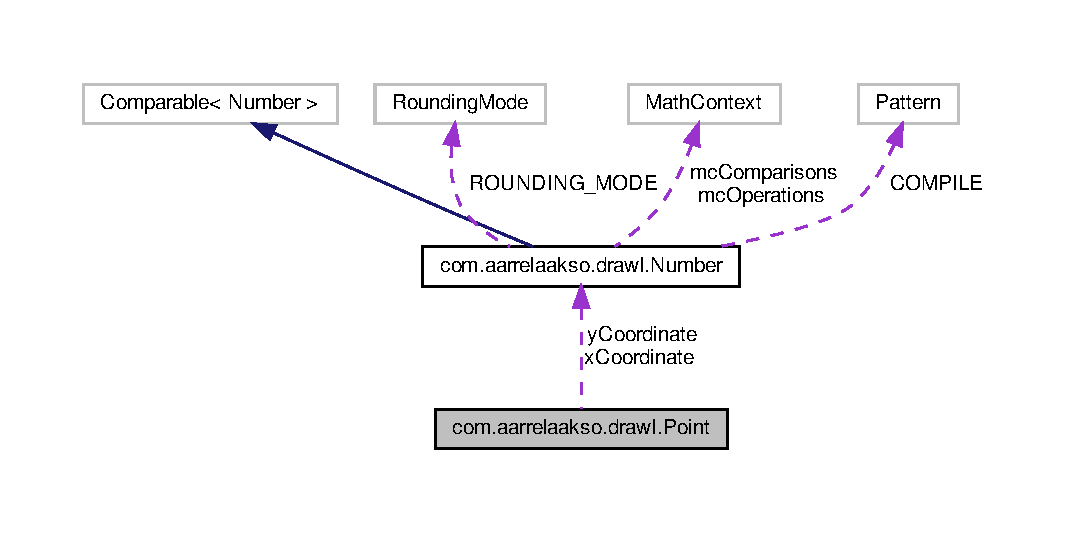
\includegraphics[width=350pt]{d8/d8b/classcom_1_1aarrelaakso_1_1drawl_1_1_point__coll__graph}
\end{center}
\end{figure}
\subsection*{Protected Member Functions}
\begin{DoxyCompactItemize}
\item 
\hyperlink{classcom_1_1aarrelaakso_1_1drawl_1_1_point_a1eb402d4971df738ea66227c7c12cb70}{Point} (final \hyperlink{interfacecom_1_1aarrelaakso_1_1drawl_1_1_number}{Number} \hyperlink{classcom_1_1aarrelaakso_1_1drawl_1_1_point_aa5144c5cca82c86f845bead6d4a51041}{x\+Coordinate}, final \hyperlink{interfacecom_1_1aarrelaakso_1_1drawl_1_1_number}{Number} \hyperlink{classcom_1_1aarrelaakso_1_1drawl_1_1_point_ab84afea50a66677c32ed2fd3100838c7}{y\+Coordinate})
\begin{DoxyCompactList}\small\item\em Constructs a new \hyperlink{classcom_1_1aarrelaakso_1_1drawl_1_1_point}{Point} object. \end{DoxyCompactList}\item 
\hyperlink{classcom_1_1aarrelaakso_1_1drawl_1_1_point_afb3376a5897946911a2230562fff07cf}{Point} (@Not\+Null final Integer \hyperlink{classcom_1_1aarrelaakso_1_1drawl_1_1_point_aa5144c5cca82c86f845bead6d4a51041}{x\+Coordinate}, @Not\+Null final Integer \hyperlink{classcom_1_1aarrelaakso_1_1drawl_1_1_point_ab84afea50a66677c32ed2fd3100838c7}{y\+Coordinate})
\item 
\hyperlink{interfacecom_1_1aarrelaakso_1_1drawl_1_1_number}{Number} \hyperlink{classcom_1_1aarrelaakso_1_1drawl_1_1_point_a39d39c84f2d05c9a2551cbc584c47bfc}{getX} ()
\begin{DoxyCompactList}\small\item\em Gets the x coordinate of this \hyperlink{classcom_1_1aarrelaakso_1_1drawl_1_1_point}{Point}. \end{DoxyCompactList}\item 
void \hyperlink{classcom_1_1aarrelaakso_1_1drawl_1_1_point_acf1cca24c7cf879f402e1b549a5e3864}{setX} (final \hyperlink{interfacecom_1_1aarrelaakso_1_1drawl_1_1_number}{Number} x)
\begin{DoxyCompactList}\small\item\em Sets the x coordinate of this \hyperlink{classcom_1_1aarrelaakso_1_1drawl_1_1_point}{Point}. \end{DoxyCompactList}\item 
\hyperlink{interfacecom_1_1aarrelaakso_1_1drawl_1_1_number}{Number} \hyperlink{classcom_1_1aarrelaakso_1_1drawl_1_1_point_a8247f55c36600e067be27a1586255767}{getY} ()
\begin{DoxyCompactList}\small\item\em Gets the y coordinate of this \hyperlink{classcom_1_1aarrelaakso_1_1drawl_1_1_point}{Point}. \end{DoxyCompactList}\end{DoxyCompactItemize}
\subsection*{Package Functions}
\begin{DoxyCompactItemize}
\item 
void \hyperlink{classcom_1_1aarrelaakso_1_1drawl_1_1_point_a713f16e843349993ac2b79bc05b5aeb6}{setY} (final \hyperlink{interfacecom_1_1aarrelaakso_1_1drawl_1_1_number}{Number} y)
\begin{DoxyCompactList}\small\item\em Sets the y coordinate of this \hyperlink{classcom_1_1aarrelaakso_1_1drawl_1_1_point}{Point}. \end{DoxyCompactList}\end{DoxyCompactItemize}
\subsection*{Private Attributes}
\begin{DoxyCompactItemize}
\item 
\hyperlink{interfacecom_1_1aarrelaakso_1_1drawl_1_1_number}{Number} \hyperlink{classcom_1_1aarrelaakso_1_1drawl_1_1_point_aa5144c5cca82c86f845bead6d4a51041}{x\+Coordinate}
\item 
\hyperlink{interfacecom_1_1aarrelaakso_1_1drawl_1_1_number}{Number} \hyperlink{classcom_1_1aarrelaakso_1_1drawl_1_1_point_ab84afea50a66677c32ed2fd3100838c7}{y\+Coordinate}
\end{DoxyCompactItemize}


\subsection{Detailed Description}
Represents a point on the drawing canvas. 

\subsection{Constructor \& Destructor Documentation}
\mbox{\Hypertarget{classcom_1_1aarrelaakso_1_1drawl_1_1_point_a1eb402d4971df738ea66227c7c12cb70}\label{classcom_1_1aarrelaakso_1_1drawl_1_1_point_a1eb402d4971df738ea66227c7c12cb70}} 
\index{com\+::aarrelaakso\+::drawl\+::\+Point@{com\+::aarrelaakso\+::drawl\+::\+Point}!Point@{Point}}
\index{Point@{Point}!com\+::aarrelaakso\+::drawl\+::\+Point@{com\+::aarrelaakso\+::drawl\+::\+Point}}
\subsubsection{\texorpdfstring{Point()}{Point()}\hspace{0.1cm}{\footnotesize\ttfamily [1/2]}}
{\footnotesize\ttfamily com.\+aarrelaakso.\+drawl.\+Point.\+Point (\begin{DoxyParamCaption}\item[{final \hyperlink{interfacecom_1_1aarrelaakso_1_1drawl_1_1_number}{Number}}]{x\+Coordinate,  }\item[{final \hyperlink{interfacecom_1_1aarrelaakso_1_1drawl_1_1_number}{Number}}]{y\+Coordinate }\end{DoxyParamCaption})\hspace{0.3cm}{\ttfamily [protected]}}



Constructs a new \hyperlink{classcom_1_1aarrelaakso_1_1drawl_1_1_point}{Point} object. 


\begin{DoxyParams}{Parameters}
{\em x\+Coordinate} & \\
\hline
{\em y\+Coordinate} & \\
\hline
\end{DoxyParams}
\mbox{\Hypertarget{classcom_1_1aarrelaakso_1_1drawl_1_1_point_afb3376a5897946911a2230562fff07cf}\label{classcom_1_1aarrelaakso_1_1drawl_1_1_point_afb3376a5897946911a2230562fff07cf}} 
\index{com\+::aarrelaakso\+::drawl\+::\+Point@{com\+::aarrelaakso\+::drawl\+::\+Point}!Point@{Point}}
\index{Point@{Point}!com\+::aarrelaakso\+::drawl\+::\+Point@{com\+::aarrelaakso\+::drawl\+::\+Point}}
\subsubsection{\texorpdfstring{Point()}{Point()}\hspace{0.1cm}{\footnotesize\ttfamily [2/2]}}
{\footnotesize\ttfamily com.\+aarrelaakso.\+drawl.\+Point.\+Point (\begin{DoxyParamCaption}\item[{@Not\+Null final Integer}]{x\+Coordinate,  }\item[{@Not\+Null final Integer}]{y\+Coordinate }\end{DoxyParamCaption})\hspace{0.3cm}{\ttfamily [protected]}}



\subsection{Member Function Documentation}
\mbox{\Hypertarget{classcom_1_1aarrelaakso_1_1drawl_1_1_point_a39d39c84f2d05c9a2551cbc584c47bfc}\label{classcom_1_1aarrelaakso_1_1drawl_1_1_point_a39d39c84f2d05c9a2551cbc584c47bfc}} 
\index{com\+::aarrelaakso\+::drawl\+::\+Point@{com\+::aarrelaakso\+::drawl\+::\+Point}!getX@{getX}}
\index{getX@{getX}!com\+::aarrelaakso\+::drawl\+::\+Point@{com\+::aarrelaakso\+::drawl\+::\+Point}}
\subsubsection{\texorpdfstring{get\+X()}{getX()}}
{\footnotesize\ttfamily \hyperlink{interfacecom_1_1aarrelaakso_1_1drawl_1_1_number}{Number} com.\+aarrelaakso.\+drawl.\+Point.\+getX (\begin{DoxyParamCaption}{ }\end{DoxyParamCaption})\hspace{0.3cm}{\ttfamily [protected]}}



Gets the x coordinate of this \hyperlink{classcom_1_1aarrelaakso_1_1drawl_1_1_point}{Point}. 

\begin{DoxyReturn}{Returns}

\end{DoxyReturn}
\begin{DoxyAuthor}{Author}
Aarre Laakso 
\end{DoxyAuthor}
\begin{DoxyVersion}{Version}
1, 05/08/2020 
\end{DoxyVersion}
\begin{DoxySince}{Since}
05/08/2020 
\end{DoxySince}
\mbox{\Hypertarget{classcom_1_1aarrelaakso_1_1drawl_1_1_point_a8247f55c36600e067be27a1586255767}\label{classcom_1_1aarrelaakso_1_1drawl_1_1_point_a8247f55c36600e067be27a1586255767}} 
\index{com\+::aarrelaakso\+::drawl\+::\+Point@{com\+::aarrelaakso\+::drawl\+::\+Point}!getY@{getY}}
\index{getY@{getY}!com\+::aarrelaakso\+::drawl\+::\+Point@{com\+::aarrelaakso\+::drawl\+::\+Point}}
\subsubsection{\texorpdfstring{get\+Y()}{getY()}}
{\footnotesize\ttfamily \hyperlink{interfacecom_1_1aarrelaakso_1_1drawl_1_1_number}{Number} com.\+aarrelaakso.\+drawl.\+Point.\+getY (\begin{DoxyParamCaption}{ }\end{DoxyParamCaption})\hspace{0.3cm}{\ttfamily [protected]}}



Gets the y coordinate of this \hyperlink{classcom_1_1aarrelaakso_1_1drawl_1_1_point}{Point}. 

\begin{DoxyReturn}{Returns}

\end{DoxyReturn}
\begin{DoxyAuthor}{Author}
Aarre Laakso 
\end{DoxyAuthor}
\begin{DoxyVersion}{Version}
1, 05/08/2020 
\end{DoxyVersion}
\begin{DoxySince}{Since}
05/08/2020 
\end{DoxySince}
\mbox{\Hypertarget{classcom_1_1aarrelaakso_1_1drawl_1_1_point_acf1cca24c7cf879f402e1b549a5e3864}\label{classcom_1_1aarrelaakso_1_1drawl_1_1_point_acf1cca24c7cf879f402e1b549a5e3864}} 
\index{com\+::aarrelaakso\+::drawl\+::\+Point@{com\+::aarrelaakso\+::drawl\+::\+Point}!setX@{setX}}
\index{setX@{setX}!com\+::aarrelaakso\+::drawl\+::\+Point@{com\+::aarrelaakso\+::drawl\+::\+Point}}
\subsubsection{\texorpdfstring{set\+X()}{setX()}}
{\footnotesize\ttfamily void com.\+aarrelaakso.\+drawl.\+Point.\+setX (\begin{DoxyParamCaption}\item[{final \hyperlink{interfacecom_1_1aarrelaakso_1_1drawl_1_1_number}{Number}}]{x }\end{DoxyParamCaption})\hspace{0.3cm}{\ttfamily [protected]}}



Sets the x coordinate of this \hyperlink{classcom_1_1aarrelaakso_1_1drawl_1_1_point}{Point}. 


\begin{DoxyParams}{Parameters}
{\em x} & the new x coordinate of this \hyperlink{classcom_1_1aarrelaakso_1_1drawl_1_1_point}{Point}. \\
\hline
\end{DoxyParams}
\begin{DoxyAuthor}{Author}
Aarre Laakso 
\end{DoxyAuthor}
\begin{DoxyVersion}{Version}
1, 05/08/2020 
\end{DoxyVersion}
\begin{DoxySince}{Since}
05/08/2020 
\end{DoxySince}
\mbox{\Hypertarget{classcom_1_1aarrelaakso_1_1drawl_1_1_point_a713f16e843349993ac2b79bc05b5aeb6}\label{classcom_1_1aarrelaakso_1_1drawl_1_1_point_a713f16e843349993ac2b79bc05b5aeb6}} 
\index{com\+::aarrelaakso\+::drawl\+::\+Point@{com\+::aarrelaakso\+::drawl\+::\+Point}!setY@{setY}}
\index{setY@{setY}!com\+::aarrelaakso\+::drawl\+::\+Point@{com\+::aarrelaakso\+::drawl\+::\+Point}}
\subsubsection{\texorpdfstring{set\+Y()}{setY()}}
{\footnotesize\ttfamily void com.\+aarrelaakso.\+drawl.\+Point.\+setY (\begin{DoxyParamCaption}\item[{final \hyperlink{interfacecom_1_1aarrelaakso_1_1drawl_1_1_number}{Number}}]{y }\end{DoxyParamCaption})\hspace{0.3cm}{\ttfamily [package]}}



Sets the y coordinate of this \hyperlink{classcom_1_1aarrelaakso_1_1drawl_1_1_point}{Point}. 


\begin{DoxyParams}{Parameters}
{\em y} & the new y coordinate of this \hyperlink{classcom_1_1aarrelaakso_1_1drawl_1_1_point}{Point}. \\
\hline
\end{DoxyParams}
\begin{DoxyAuthor}{Author}
Aarre Laakso 
\end{DoxyAuthor}
\begin{DoxyVersion}{Version}
1, 05/08/2020 
\end{DoxyVersion}
\begin{DoxySince}{Since}
05/08/2020 
\end{DoxySince}


\subsection{Member Data Documentation}
\mbox{\Hypertarget{classcom_1_1aarrelaakso_1_1drawl_1_1_point_aa5144c5cca82c86f845bead6d4a51041}\label{classcom_1_1aarrelaakso_1_1drawl_1_1_point_aa5144c5cca82c86f845bead6d4a51041}} 
\index{com\+::aarrelaakso\+::drawl\+::\+Point@{com\+::aarrelaakso\+::drawl\+::\+Point}!x\+Coordinate@{x\+Coordinate}}
\index{x\+Coordinate@{x\+Coordinate}!com\+::aarrelaakso\+::drawl\+::\+Point@{com\+::aarrelaakso\+::drawl\+::\+Point}}
\subsubsection{\texorpdfstring{x\+Coordinate}{xCoordinate}}
{\footnotesize\ttfamily \hyperlink{interfacecom_1_1aarrelaakso_1_1drawl_1_1_number}{Number} com.\+aarrelaakso.\+drawl.\+Point.\+x\+Coordinate\hspace{0.3cm}{\ttfamily [private]}}

\mbox{\Hypertarget{classcom_1_1aarrelaakso_1_1drawl_1_1_point_ab84afea50a66677c32ed2fd3100838c7}\label{classcom_1_1aarrelaakso_1_1drawl_1_1_point_ab84afea50a66677c32ed2fd3100838c7}} 
\index{com\+::aarrelaakso\+::drawl\+::\+Point@{com\+::aarrelaakso\+::drawl\+::\+Point}!y\+Coordinate@{y\+Coordinate}}
\index{y\+Coordinate@{y\+Coordinate}!com\+::aarrelaakso\+::drawl\+::\+Point@{com\+::aarrelaakso\+::drawl\+::\+Point}}
\subsubsection{\texorpdfstring{y\+Coordinate}{yCoordinate}}
{\footnotesize\ttfamily \hyperlink{interfacecom_1_1aarrelaakso_1_1drawl_1_1_number}{Number} com.\+aarrelaakso.\+drawl.\+Point.\+y\+Coordinate\hspace{0.3cm}{\ttfamily [private]}}



The documentation for this class was generated from the following file\+:\begin{DoxyCompactItemize}
\item 
/mnt/d/\+One\+Drive/\+Documents/src/drawl/src/main/java/com/aarrelaakso/drawl/\hyperlink{_point_8java}{Point.\+java}\end{DoxyCompactItemize}

\hypertarget{classcom_1_1aarrelaakso_1_1drawl_1_1examples_1_1_policy_priorities}{}\section{com.\+aarrelaakso.\+drawl.\+examples.\+Policy\+Priorities Class Reference}
\label{classcom_1_1aarrelaakso_1_1drawl_1_1examples_1_1_policy_priorities}\index{com.\+aarrelaakso.\+drawl.\+examples.\+Policy\+Priorities@{com.\+aarrelaakso.\+drawl.\+examples.\+Policy\+Priorities}}
\subsection*{Static Public Member Functions}
\begin{DoxyCompactItemize}
\item 
static void \hyperlink{classcom_1_1aarrelaakso_1_1drawl_1_1examples_1_1_policy_priorities_a8e93196f3da008884909a2dabec04d3f}{main} (final String\mbox{[}$\,$\mbox{]} args)  throws I\+O\+Exception     
\end{DoxyCompactItemize}


\subsection{Member Function Documentation}
\mbox{\Hypertarget{classcom_1_1aarrelaakso_1_1drawl_1_1examples_1_1_policy_priorities_a8e93196f3da008884909a2dabec04d3f}\label{classcom_1_1aarrelaakso_1_1drawl_1_1examples_1_1_policy_priorities_a8e93196f3da008884909a2dabec04d3f}} 
\index{com\+::aarrelaakso\+::drawl\+::examples\+::\+Policy\+Priorities@{com\+::aarrelaakso\+::drawl\+::examples\+::\+Policy\+Priorities}!main@{main}}
\index{main@{main}!com\+::aarrelaakso\+::drawl\+::examples\+::\+Policy\+Priorities@{com\+::aarrelaakso\+::drawl\+::examples\+::\+Policy\+Priorities}}
\subsubsection{\texorpdfstring{main()}{main()}}
{\footnotesize\ttfamily static void com.\+aarrelaakso.\+drawl.\+examples.\+Policy\+Priorities.\+main (\begin{DoxyParamCaption}\item[{final String \mbox{[}$\,$\mbox{]}}]{args }\end{DoxyParamCaption}) throws I\+O\+Exception\hspace{0.3cm}{\ttfamily [static]}}



The documentation for this class was generated from the following file\+:\begin{DoxyCompactItemize}
\item 
/mnt/d/\+One\+Drive/\+Documents/src/drawl/src/main/java/com/aarrelaakso/drawl/examples/\hyperlink{_policy_priorities_8java}{Policy\+Priorities.\+java}\end{DoxyCompactItemize}

\hypertarget{classcom_1_1aarrelaakso_1_1drawl_1_1_rectangle}{}\section{com.\+aarrelaakso.\+drawl.\+Rectangle Class Reference}
\label{classcom_1_1aarrelaakso_1_1drawl_1_1_rectangle}\index{com.\+aarrelaakso.\+drawl.\+Rectangle@{com.\+aarrelaakso.\+drawl.\+Rectangle}}


Inheritance diagram for com.\+aarrelaakso.\+drawl.\+Rectangle\+:\nopagebreak
\begin{figure}[H]
\begin{center}
\leavevmode
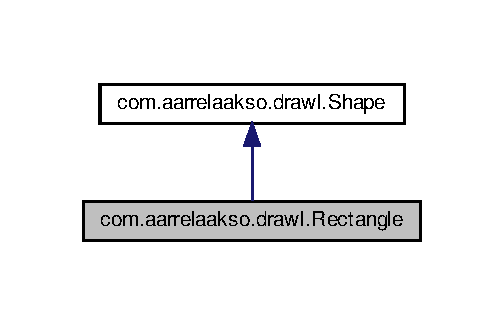
\includegraphics[width=242pt]{classcom_1_1aarrelaakso_1_1drawl_1_1_rectangle__inherit__graph}
\end{center}
\end{figure}


Collaboration diagram for com.\+aarrelaakso.\+drawl.\+Rectangle\+:\nopagebreak
\begin{figure}[H]
\begin{center}
\leavevmode
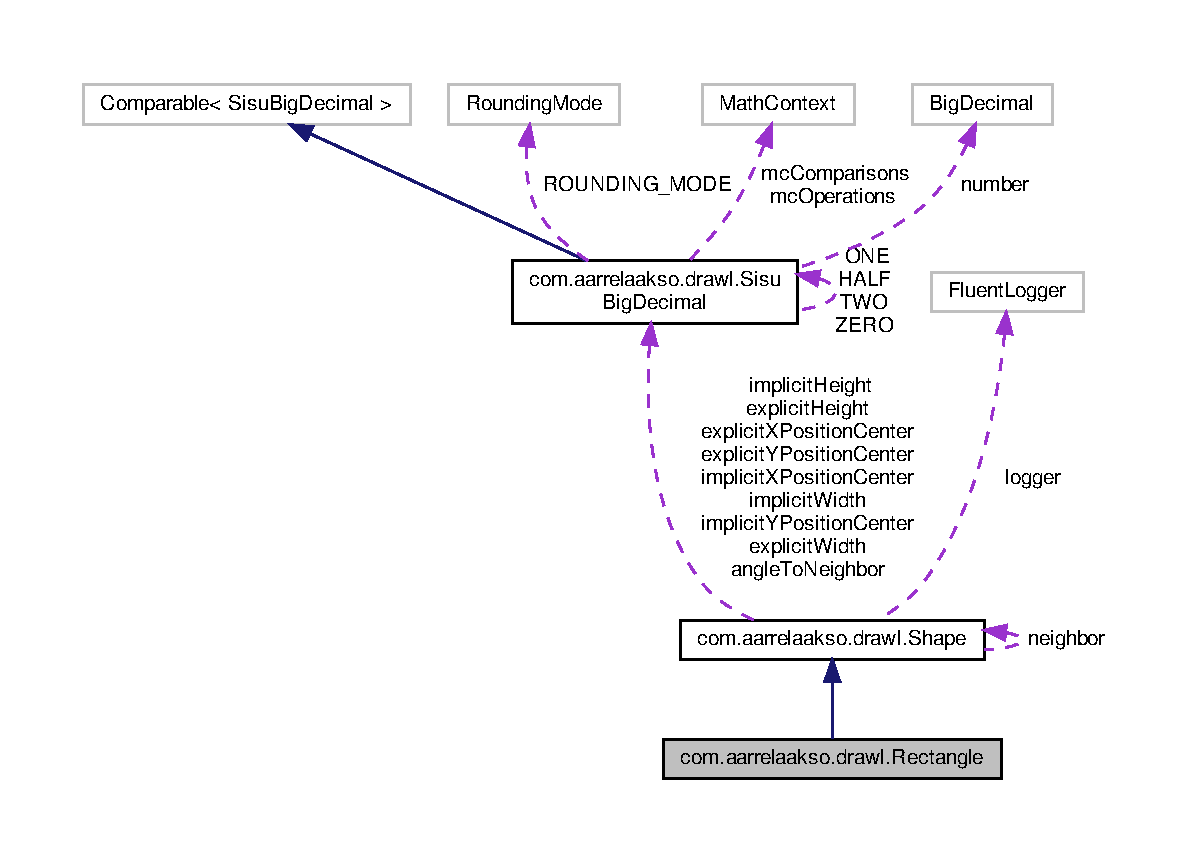
\includegraphics[width=350pt]{classcom_1_1aarrelaakso_1_1drawl_1_1_rectangle__coll__graph}
\end{center}
\end{figure}
\subsection*{Public Member Functions}
\begin{DoxyCompactItemize}
\item 
\hyperlink{classcom_1_1aarrelaakso_1_1drawl_1_1_rectangle_aa595469acf7ff55a123ba946633c573f}{Rectangle} ()
\item 
\hyperlink{classcom_1_1aarrelaakso_1_1drawl_1_1_rectangle_ab0fbbbcfd8392e59ffdb4cb78f3447ff}{Rectangle} (Double aspect\+Ratio)
\item 
String \hyperlink{classcom_1_1aarrelaakso_1_1drawl_1_1_rectangle_a175f326e054b08426648a81a246904a7}{get\+S\+VG} ()
\item 
\hyperlink{classcom_1_1aarrelaakso_1_1drawl_1_1_shape}{Shape} \hyperlink{classcom_1_1aarrelaakso_1_1drawl_1_1_shape_acebea2aa57031322323c9bf50ee447db}{get\+Above} ()
\item 
\hyperlink{classcom_1_1aarrelaakso_1_1drawl_1_1_shape}{Shape} \hyperlink{classcom_1_1aarrelaakso_1_1drawl_1_1_shape_a53de5ab609d879719cd3b372dfe8df58}{get\+Below} ()
\item 
String \hyperlink{classcom_1_1aarrelaakso_1_1drawl_1_1_shape_a0d9a33a3e151aaceeec140bea343a650}{get\+Fill} ()
\item 
\hyperlink{classcom_1_1aarrelaakso_1_1drawl_1_1_shape}{Shape} \hyperlink{classcom_1_1aarrelaakso_1_1drawl_1_1_shape_a2b19d5964ac46d545a7bae3133df6532}{get\+Left\+Of} ()
\item 
\hyperlink{classcom_1_1aarrelaakso_1_1drawl_1_1_shape}{Shape} \hyperlink{classcom_1_1aarrelaakso_1_1drawl_1_1_shape_a1ad573b06f341aa79f6a255a476ae6e4}{get\+Right\+Of} ()
\item 
String \hyperlink{classcom_1_1aarrelaakso_1_1drawl_1_1_shape_a4e1d54c7e161e3af5053939ddefdf9e6}{get\+Stroke} ()
\item 
void \hyperlink{classcom_1_1aarrelaakso_1_1drawl_1_1_shape_a942b3cf3365498dc1ac6b0309ce33b86}{set\+Above} (\hyperlink{classcom_1_1aarrelaakso_1_1drawl_1_1_shape}{Shape} shape)
\item 
void \hyperlink{classcom_1_1aarrelaakso_1_1drawl_1_1_shape_aa0ec0030515b5096820e4dd030c0b320}{set\+Below} (\hyperlink{classcom_1_1aarrelaakso_1_1drawl_1_1_shape}{Shape} shape)
\item 
void \hyperlink{classcom_1_1aarrelaakso_1_1drawl_1_1_shape_a2a2868c85bfbf4d2940d929950001b3d}{set\+Fill} (String s)
\item 
void \hyperlink{classcom_1_1aarrelaakso_1_1drawl_1_1_shape_aad14fa860ab74cfa90815f56cf4c3ecf}{set\+Left\+Of} (\hyperlink{classcom_1_1aarrelaakso_1_1drawl_1_1_shape}{Shape} shape)
\item 
void \hyperlink{classcom_1_1aarrelaakso_1_1drawl_1_1_shape_a09e1586ce85c1d964cc3b7ce94bc5d4c}{set\+Right\+Of} (\hyperlink{classcom_1_1aarrelaakso_1_1drawl_1_1_shape}{Shape} shape)
\item 
void \hyperlink{classcom_1_1aarrelaakso_1_1drawl_1_1_shape_a3930f6fe72f6c5e0c0aa4c25ffbf18ff}{set\+Stroke} (String s)
\end{DoxyCompactItemize}
\subsection*{Protected Member Functions}
\begin{DoxyCompactItemize}
\item 
\hyperlink{classcom_1_1aarrelaakso_1_1drawl_1_1_rectangle_a178c07a0610409258818f61ae332d85a}{Rectangle} (Integer \hyperlink{classcom_1_1aarrelaakso_1_1drawl_1_1_shape_a100066b3ccbb6e88080211b00ad8ebb9}{implicit\+Width}, Integer \hyperlink{classcom_1_1aarrelaakso_1_1drawl_1_1_shape_ab374c520d98692018b1a5866acd33849}{implicit\+Height})
\item 
\hyperlink{classcom_1_1aarrelaakso_1_1drawl_1_1_rectangle_aa5cd32bd84c1b9f0dd53757d2b4460f2}{Rectangle} (\hyperlink{classcom_1_1aarrelaakso_1_1drawl_1_1_sisu_big_decimal}{Sisu\+Big\+Decimal} \hyperlink{classcom_1_1aarrelaakso_1_1drawl_1_1_shape_a100066b3ccbb6e88080211b00ad8ebb9}{implicit\+Width}, \hyperlink{classcom_1_1aarrelaakso_1_1drawl_1_1_sisu_big_decimal}{Sisu\+Big\+Decimal} \hyperlink{classcom_1_1aarrelaakso_1_1drawl_1_1_shape_ab374c520d98692018b1a5866acd33849}{implicit\+Height})
\item 
\hyperlink{classcom_1_1aarrelaakso_1_1drawl_1_1_sisu_big_decimal}{Sisu\+Big\+Decimal} \hyperlink{classcom_1_1aarrelaakso_1_1drawl_1_1_shape_aa3857406bc4f6c7373f1cd7cbe16dfd9}{get\+Explicit\+Half\+Height} ()
\item 
\hyperlink{classcom_1_1aarrelaakso_1_1drawl_1_1_sisu_big_decimal}{Sisu\+Big\+Decimal} \hyperlink{classcom_1_1aarrelaakso_1_1drawl_1_1_shape_a4fba348eaeef3c258aa7443410137ad7}{get\+Explicit\+Half\+Width} ()
\item 
\hyperlink{classcom_1_1aarrelaakso_1_1drawl_1_1_sisu_big_decimal}{Sisu\+Big\+Decimal} \hyperlink{classcom_1_1aarrelaakso_1_1drawl_1_1_shape_a0a263872f3a0bd19822415420e132a07}{get\+Explicit\+Height} ()
\item 
\hyperlink{classcom_1_1aarrelaakso_1_1drawl_1_1_sisu_big_decimal}{Sisu\+Big\+Decimal} \hyperlink{classcom_1_1aarrelaakso_1_1drawl_1_1_shape_a398f978e0902c270a8f61d6827bcfd8f}{get\+Explicit\+Width} ()
\item 
\hyperlink{classcom_1_1aarrelaakso_1_1drawl_1_1_sisu_big_decimal}{Sisu\+Big\+Decimal} \hyperlink{classcom_1_1aarrelaakso_1_1drawl_1_1_shape_a079e4ec300c2ab3cd2514230b7428ea4}{get\+Explicit\+X\+Position\+Center} ()
\item 
\hyperlink{classcom_1_1aarrelaakso_1_1drawl_1_1_sisu_big_decimal}{Sisu\+Big\+Decimal} \hyperlink{classcom_1_1aarrelaakso_1_1drawl_1_1_shape_a4e26548d18a063bff6bb0781526b909f}{get\+Explicit\+X\+Position\+Left} ()
\item 
\hyperlink{classcom_1_1aarrelaakso_1_1drawl_1_1_sisu_big_decimal}{Sisu\+Big\+Decimal} \hyperlink{classcom_1_1aarrelaakso_1_1drawl_1_1_shape_adfeaa06d8a6943d8f5bc90e91f0b4fac}{get\+Explicit\+Y\+Position\+Bottom} ()
\item 
\hyperlink{classcom_1_1aarrelaakso_1_1drawl_1_1_sisu_big_decimal}{Sisu\+Big\+Decimal} \hyperlink{classcom_1_1aarrelaakso_1_1drawl_1_1_shape_a6499eaa6fd9cdef3d77fe20a5b039401}{get\+Explicit\+Y\+Position\+Center} ()
\item 
\hyperlink{classcom_1_1aarrelaakso_1_1drawl_1_1_sisu_big_decimal}{Sisu\+Big\+Decimal} \hyperlink{classcom_1_1aarrelaakso_1_1drawl_1_1_shape_af5d7293539d67234c9941e6abc3e642b}{get\+Explicit\+Y\+Position\+Top} ()
\item 
\hyperlink{classcom_1_1aarrelaakso_1_1drawl_1_1_sisu_big_decimal}{Sisu\+Big\+Decimal} \hyperlink{classcom_1_1aarrelaakso_1_1drawl_1_1_shape_a33908342a13df06645b6ab7c1fd7a801}{get\+Implicit\+Half\+Height} ()
\item 
\hyperlink{classcom_1_1aarrelaakso_1_1drawl_1_1_sisu_big_decimal}{Sisu\+Big\+Decimal} \hyperlink{classcom_1_1aarrelaakso_1_1drawl_1_1_shape_a46d1d2823bc131d796a6a41383334d85}{get\+Implicit\+Half\+Width} ()
\item 
\hyperlink{classcom_1_1aarrelaakso_1_1drawl_1_1_sisu_big_decimal}{Sisu\+Big\+Decimal} \hyperlink{classcom_1_1aarrelaakso_1_1drawl_1_1_shape_a76f8b3c8365af3e5800ad06113b3e507}{get\+Implicit\+Height} ()
\item 
\hyperlink{classcom_1_1aarrelaakso_1_1drawl_1_1_sisu_big_decimal}{Sisu\+Big\+Decimal} \hyperlink{classcom_1_1aarrelaakso_1_1drawl_1_1_shape_af6a043538a5aba4f4b3eb7278206a841}{get\+Implicit\+Width} ()
\item 
\hyperlink{classcom_1_1aarrelaakso_1_1drawl_1_1_sisu_big_decimal}{Sisu\+Big\+Decimal} \hyperlink{classcom_1_1aarrelaakso_1_1drawl_1_1_shape_a3bde9d5b2cc582ddb6c521b122c40ff8}{get\+Implicit\+X\+Maximum} ()
\item 
\hyperlink{classcom_1_1aarrelaakso_1_1drawl_1_1_sisu_big_decimal}{Sisu\+Big\+Decimal} \hyperlink{classcom_1_1aarrelaakso_1_1drawl_1_1_shape_af0ceac29118047c73bd3ff308a71c36f}{get\+Implicit\+X\+Minimum} ()
\item 
\hyperlink{classcom_1_1aarrelaakso_1_1drawl_1_1_sisu_big_decimal}{Sisu\+Big\+Decimal} \hyperlink{classcom_1_1aarrelaakso_1_1drawl_1_1_shape_a50c12c30790bd28ec0b71b58f59b1e96}{get\+Implicit\+X\+Position\+Center} ()
\item 
\hyperlink{classcom_1_1aarrelaakso_1_1drawl_1_1_sisu_big_decimal}{Sisu\+Big\+Decimal} \hyperlink{classcom_1_1aarrelaakso_1_1drawl_1_1_shape_ad9b2aee9937d5f034f7f4a2a1d979260}{get\+Implicit\+X\+Position\+Left} ()
\item 
\hyperlink{classcom_1_1aarrelaakso_1_1drawl_1_1_sisu_big_decimal}{Sisu\+Big\+Decimal} \hyperlink{classcom_1_1aarrelaakso_1_1drawl_1_1_shape_a7a4579f2966a3d5ebbfa46b5b2528f9d}{get\+Implicit\+Y\+Maximum} ()
\item 
\hyperlink{classcom_1_1aarrelaakso_1_1drawl_1_1_sisu_big_decimal}{Sisu\+Big\+Decimal} \hyperlink{classcom_1_1aarrelaakso_1_1drawl_1_1_shape_aa0877965f7f172378e87ba69f27c7ad6}{get\+Implicit\+Y\+Minimum} ()
\item 
\hyperlink{classcom_1_1aarrelaakso_1_1drawl_1_1_sisu_big_decimal}{Sisu\+Big\+Decimal} \hyperlink{classcom_1_1aarrelaakso_1_1drawl_1_1_shape_a5116673c093c60f66bba9fddf9533db6}{get\+Implicit\+Y\+Position\+Bottom} ()
\item 
\hyperlink{classcom_1_1aarrelaakso_1_1drawl_1_1_sisu_big_decimal}{Sisu\+Big\+Decimal} \hyperlink{classcom_1_1aarrelaakso_1_1drawl_1_1_shape_ad10def6c8dd7cbe03c281817406ab461}{get\+Implicit\+Y\+Position\+Center} ()
\item 
\hyperlink{classcom_1_1aarrelaakso_1_1drawl_1_1_sisu_big_decimal}{Sisu\+Big\+Decimal} \hyperlink{classcom_1_1aarrelaakso_1_1drawl_1_1_shape_a5ffc02627cca0723e3555b5d04ba2b75}{get\+Implicit\+Y\+Position\+Top} ()
\item 
void \hyperlink{classcom_1_1aarrelaakso_1_1drawl_1_1_shape_a37e0c4b85c07c4c87a24609ae1cb50a5}{set\+Explicit\+Height} (@Nullable \hyperlink{classcom_1_1aarrelaakso_1_1drawl_1_1_sisu_big_decimal}{Sisu\+Big\+Decimal} height)
\item 
void \hyperlink{classcom_1_1aarrelaakso_1_1drawl_1_1_shape_a976c002388892d227697cab39c1e5724}{set\+Explicit\+Width} (@Nullable \hyperlink{classcom_1_1aarrelaakso_1_1drawl_1_1_sisu_big_decimal}{Sisu\+Big\+Decimal} width)
\item 
void \hyperlink{classcom_1_1aarrelaakso_1_1drawl_1_1_shape_a8e4c74480fede49f44519554136c12b0}{set\+Explicit\+X\+Position\+Center} (\hyperlink{classcom_1_1aarrelaakso_1_1drawl_1_1_sisu_big_decimal}{Sisu\+Big\+Decimal} x)
\item 
void \hyperlink{classcom_1_1aarrelaakso_1_1drawl_1_1_shape_aa7855df6d98b3bfa556b7d857755181b}{set\+Explicit\+X\+Position\+Center} (Integer x)
\item 
void \hyperlink{classcom_1_1aarrelaakso_1_1drawl_1_1_shape_af8af5129e3e61324439a1035428016a2}{set\+Explicit\+Y\+Position} (Integer y)
\item 
void \hyperlink{classcom_1_1aarrelaakso_1_1drawl_1_1_shape_a0ddc58345fca924e973fac474955ef14}{set\+Explicit\+Y\+Position\+Center} (\hyperlink{classcom_1_1aarrelaakso_1_1drawl_1_1_sisu_big_decimal}{Sisu\+Big\+Decimal} y)
\item 
final void \hyperlink{classcom_1_1aarrelaakso_1_1drawl_1_1_shape_ad41ecfc8ce74638066d8a21c97e3f399}{set\+Implicit\+Height} (\hyperlink{classcom_1_1aarrelaakso_1_1drawl_1_1_sisu_big_decimal}{Sisu\+Big\+Decimal} \hyperlink{classcom_1_1aarrelaakso_1_1drawl_1_1_shape_ab374c520d98692018b1a5866acd33849}{implicit\+Height})
\item 
final void \hyperlink{classcom_1_1aarrelaakso_1_1drawl_1_1_shape_a6ec4c2bd26d08f0a1545bd1d5f47c05a}{set\+Implicit\+Width} (\hyperlink{classcom_1_1aarrelaakso_1_1drawl_1_1_sisu_big_decimal}{Sisu\+Big\+Decimal} \hyperlink{classcom_1_1aarrelaakso_1_1drawl_1_1_shape_a100066b3ccbb6e88080211b00ad8ebb9}{implicit\+Width})
\item 
void \hyperlink{classcom_1_1aarrelaakso_1_1drawl_1_1_shape_a4fbc0d430cfe312e018e4ec58f726842}{set\+Implicit\+X\+Position\+Center} (\hyperlink{classcom_1_1aarrelaakso_1_1drawl_1_1_sisu_big_decimal}{Sisu\+Big\+Decimal} x)
\item 
void \hyperlink{classcom_1_1aarrelaakso_1_1drawl_1_1_shape_ac1cf4cf6f0bcc489b996a10a600d5629}{set\+Implicit\+Y\+Position\+Center} (\hyperlink{classcom_1_1aarrelaakso_1_1drawl_1_1_sisu_big_decimal}{Sisu\+Big\+Decimal} y)
\end{DoxyCompactItemize}
\subsection*{Static Package Functions}
\begin{DoxyCompactItemize}
\item 
\hyperlink{classcom_1_1aarrelaakso_1_1drawl_1_1_shape_ad2adcb85374cf5d6d59429628314e8d1}{\mbox{[}static initializer\mbox{]}}
\end{DoxyCompactItemize}


\subsection{Constructor \& Destructor Documentation}
\mbox{\Hypertarget{classcom_1_1aarrelaakso_1_1drawl_1_1_rectangle_aa595469acf7ff55a123ba946633c573f}\label{classcom_1_1aarrelaakso_1_1drawl_1_1_rectangle_aa595469acf7ff55a123ba946633c573f}} 
\index{com\+::aarrelaakso\+::drawl\+::\+Rectangle@{com\+::aarrelaakso\+::drawl\+::\+Rectangle}!Rectangle@{Rectangle}}
\index{Rectangle@{Rectangle}!com\+::aarrelaakso\+::drawl\+::\+Rectangle@{com\+::aarrelaakso\+::drawl\+::\+Rectangle}}
\subsubsection{\texorpdfstring{Rectangle()}{Rectangle()}\hspace{0.1cm}{\footnotesize\ttfamily [1/4]}}
{\footnotesize\ttfamily com.\+aarrelaakso.\+drawl.\+Rectangle.\+Rectangle (\begin{DoxyParamCaption}{ }\end{DoxyParamCaption})}

Creates a \hyperlink{classcom_1_1aarrelaakso_1_1drawl_1_1_rectangle}{Rectangle} with the default width and height. \mbox{\Hypertarget{classcom_1_1aarrelaakso_1_1drawl_1_1_rectangle_ab0fbbbcfd8392e59ffdb4cb78f3447ff}\label{classcom_1_1aarrelaakso_1_1drawl_1_1_rectangle_ab0fbbbcfd8392e59ffdb4cb78f3447ff}} 
\index{com\+::aarrelaakso\+::drawl\+::\+Rectangle@{com\+::aarrelaakso\+::drawl\+::\+Rectangle}!Rectangle@{Rectangle}}
\index{Rectangle@{Rectangle}!com\+::aarrelaakso\+::drawl\+::\+Rectangle@{com\+::aarrelaakso\+::drawl\+::\+Rectangle}}
\subsubsection{\texorpdfstring{Rectangle()}{Rectangle()}\hspace{0.1cm}{\footnotesize\ttfamily [2/4]}}
{\footnotesize\ttfamily com.\+aarrelaakso.\+drawl.\+Rectangle.\+Rectangle (\begin{DoxyParamCaption}\item[{Double}]{aspect\+Ratio }\end{DoxyParamCaption})}

Creates a rectangle with a given aspect ratio.


\begin{DoxyParams}{Parameters}
{\em aspect\+Ratio} & The aspect ratio of the new rectangle. The aspect ratio is expressed as width over height. \\
\hline
\end{DoxyParams}
\mbox{\Hypertarget{classcom_1_1aarrelaakso_1_1drawl_1_1_rectangle_a178c07a0610409258818f61ae332d85a}\label{classcom_1_1aarrelaakso_1_1drawl_1_1_rectangle_a178c07a0610409258818f61ae332d85a}} 
\index{com\+::aarrelaakso\+::drawl\+::\+Rectangle@{com\+::aarrelaakso\+::drawl\+::\+Rectangle}!Rectangle@{Rectangle}}
\index{Rectangle@{Rectangle}!com\+::aarrelaakso\+::drawl\+::\+Rectangle@{com\+::aarrelaakso\+::drawl\+::\+Rectangle}}
\subsubsection{\texorpdfstring{Rectangle()}{Rectangle()}\hspace{0.1cm}{\footnotesize\ttfamily [3/4]}}
{\footnotesize\ttfamily com.\+aarrelaakso.\+drawl.\+Rectangle.\+Rectangle (\begin{DoxyParamCaption}\item[{Integer}]{implicit\+Width,  }\item[{Integer}]{implicit\+Height }\end{DoxyParamCaption})\hspace{0.3cm}{\ttfamily [protected]}}

Creates a new \hyperlink{classcom_1_1aarrelaakso_1_1drawl_1_1_rectangle}{Rectangle} with a given width and height.


\begin{DoxyParams}{Parameters}
{\em implicit\+Width} & the width of the new \hyperlink{classcom_1_1aarrelaakso_1_1drawl_1_1_rectangle}{Rectangle}. \\
\hline
{\em implicit\+Height} & the height of the new \hyperlink{classcom_1_1aarrelaakso_1_1drawl_1_1_rectangle}{Rectangle}. \\
\hline
\end{DoxyParams}
\mbox{\Hypertarget{classcom_1_1aarrelaakso_1_1drawl_1_1_rectangle_aa5cd32bd84c1b9f0dd53757d2b4460f2}\label{classcom_1_1aarrelaakso_1_1drawl_1_1_rectangle_aa5cd32bd84c1b9f0dd53757d2b4460f2}} 
\index{com\+::aarrelaakso\+::drawl\+::\+Rectangle@{com\+::aarrelaakso\+::drawl\+::\+Rectangle}!Rectangle@{Rectangle}}
\index{Rectangle@{Rectangle}!com\+::aarrelaakso\+::drawl\+::\+Rectangle@{com\+::aarrelaakso\+::drawl\+::\+Rectangle}}
\subsubsection{\texorpdfstring{Rectangle()}{Rectangle()}\hspace{0.1cm}{\footnotesize\ttfamily [4/4]}}
{\footnotesize\ttfamily com.\+aarrelaakso.\+drawl.\+Rectangle.\+Rectangle (\begin{DoxyParamCaption}\item[{\hyperlink{classcom_1_1aarrelaakso_1_1drawl_1_1_sisu_big_decimal}{Sisu\+Big\+Decimal}}]{implicit\+Width,  }\item[{\hyperlink{classcom_1_1aarrelaakso_1_1drawl_1_1_sisu_big_decimal}{Sisu\+Big\+Decimal}}]{implicit\+Height }\end{DoxyParamCaption})\hspace{0.3cm}{\ttfamily [protected]}}

Creates a new \hyperlink{classcom_1_1aarrelaakso_1_1drawl_1_1_rectangle}{Rectangle} with a given width and height.


\begin{DoxyParams}{Parameters}
{\em implicit\+Width} & the width of the new \hyperlink{classcom_1_1aarrelaakso_1_1drawl_1_1_rectangle}{Rectangle}. \\
\hline
{\em implicit\+Height} & the height of the new \hyperlink{classcom_1_1aarrelaakso_1_1drawl_1_1_rectangle}{Rectangle}. \\
\hline
\end{DoxyParams}


\subsection{Member Function Documentation}
\mbox{\Hypertarget{classcom_1_1aarrelaakso_1_1drawl_1_1_shape_ad2adcb85374cf5d6d59429628314e8d1}\label{classcom_1_1aarrelaakso_1_1drawl_1_1_shape_ad2adcb85374cf5d6d59429628314e8d1}} 
\index{com\+::aarrelaakso\+::drawl\+::\+Rectangle@{com\+::aarrelaakso\+::drawl\+::\+Rectangle}!\mbox{[}static initializer\mbox{]}@{[static initializer]}}
\index{\mbox{[}static initializer\mbox{]}@{[static initializer]}!com\+::aarrelaakso\+::drawl\+::\+Rectangle@{com\+::aarrelaakso\+::drawl\+::\+Rectangle}}
\subsubsection{\texorpdfstring{[static initializer]()}{[static initializer]()}}
{\footnotesize\ttfamily com.\+aarrelaakso.\+drawl.\+Shape.\mbox{[}static initializer\mbox{]} (\begin{DoxyParamCaption}{ }\end{DoxyParamCaption})\hspace{0.3cm}{\ttfamily [static]}, {\ttfamily [package]}, {\ttfamily [inherited]}}

\mbox{\Hypertarget{classcom_1_1aarrelaakso_1_1drawl_1_1_shape_acebea2aa57031322323c9bf50ee447db}\label{classcom_1_1aarrelaakso_1_1drawl_1_1_shape_acebea2aa57031322323c9bf50ee447db}} 
\index{com\+::aarrelaakso\+::drawl\+::\+Rectangle@{com\+::aarrelaakso\+::drawl\+::\+Rectangle}!get\+Above@{get\+Above}}
\index{get\+Above@{get\+Above}!com\+::aarrelaakso\+::drawl\+::\+Rectangle@{com\+::aarrelaakso\+::drawl\+::\+Rectangle}}
\subsubsection{\texorpdfstring{get\+Above()}{getAbove()}}
{\footnotesize\ttfamily \hyperlink{classcom_1_1aarrelaakso_1_1drawl_1_1_shape}{Shape} com.\+aarrelaakso.\+drawl.\+Shape.\+get\+Above (\begin{DoxyParamCaption}{ }\end{DoxyParamCaption})\hspace{0.3cm}{\ttfamily [inherited]}}

Get this \hyperlink{classcom_1_1aarrelaakso_1_1drawl_1_1_shape}{Shape}\textquotesingle{}s neighbor above (this \hyperlink{classcom_1_1aarrelaakso_1_1drawl_1_1_shape}{Shape} is below that one), if any.

\begin{DoxyReturn}{Returns}
the \hyperlink{classcom_1_1aarrelaakso_1_1drawl_1_1_shape}{Shape} to the right of this one, if any; {\ttfamily null} otherwise. 
\end{DoxyReturn}
\mbox{\Hypertarget{classcom_1_1aarrelaakso_1_1drawl_1_1_shape_a53de5ab609d879719cd3b372dfe8df58}\label{classcom_1_1aarrelaakso_1_1drawl_1_1_shape_a53de5ab609d879719cd3b372dfe8df58}} 
\index{com\+::aarrelaakso\+::drawl\+::\+Rectangle@{com\+::aarrelaakso\+::drawl\+::\+Rectangle}!get\+Below@{get\+Below}}
\index{get\+Below@{get\+Below}!com\+::aarrelaakso\+::drawl\+::\+Rectangle@{com\+::aarrelaakso\+::drawl\+::\+Rectangle}}
\subsubsection{\texorpdfstring{get\+Below()}{getBelow()}}
{\footnotesize\ttfamily \hyperlink{classcom_1_1aarrelaakso_1_1drawl_1_1_shape}{Shape} com.\+aarrelaakso.\+drawl.\+Shape.\+get\+Below (\begin{DoxyParamCaption}{ }\end{DoxyParamCaption})\hspace{0.3cm}{\ttfamily [inherited]}}

Get this \hyperlink{classcom_1_1aarrelaakso_1_1drawl_1_1_shape}{Shape}\textquotesingle{}s neighbor below (this \hyperlink{classcom_1_1aarrelaakso_1_1drawl_1_1_shape}{Shape} is below that one), if any.

\begin{DoxyReturn}{Returns}
the \hyperlink{classcom_1_1aarrelaakso_1_1drawl_1_1_shape}{Shape} to below this one, if any; {\ttfamily null} otherwise. 
\end{DoxyReturn}
\mbox{\Hypertarget{classcom_1_1aarrelaakso_1_1drawl_1_1_shape_aa3857406bc4f6c7373f1cd7cbe16dfd9}\label{classcom_1_1aarrelaakso_1_1drawl_1_1_shape_aa3857406bc4f6c7373f1cd7cbe16dfd9}} 
\index{com\+::aarrelaakso\+::drawl\+::\+Rectangle@{com\+::aarrelaakso\+::drawl\+::\+Rectangle}!get\+Explicit\+Half\+Height@{get\+Explicit\+Half\+Height}}
\index{get\+Explicit\+Half\+Height@{get\+Explicit\+Half\+Height}!com\+::aarrelaakso\+::drawl\+::\+Rectangle@{com\+::aarrelaakso\+::drawl\+::\+Rectangle}}
\subsubsection{\texorpdfstring{get\+Explicit\+Half\+Height()}{getExplicitHalfHeight()}}
{\footnotesize\ttfamily \hyperlink{classcom_1_1aarrelaakso_1_1drawl_1_1_sisu_big_decimal}{Sisu\+Big\+Decimal} com.\+aarrelaakso.\+drawl.\+Shape.\+get\+Explicit\+Half\+Height (\begin{DoxyParamCaption}{ }\end{DoxyParamCaption})\hspace{0.3cm}{\ttfamily [protected]}, {\ttfamily [inherited]}}

\mbox{\Hypertarget{classcom_1_1aarrelaakso_1_1drawl_1_1_shape_a4fba348eaeef3c258aa7443410137ad7}\label{classcom_1_1aarrelaakso_1_1drawl_1_1_shape_a4fba348eaeef3c258aa7443410137ad7}} 
\index{com\+::aarrelaakso\+::drawl\+::\+Rectangle@{com\+::aarrelaakso\+::drawl\+::\+Rectangle}!get\+Explicit\+Half\+Width@{get\+Explicit\+Half\+Width}}
\index{get\+Explicit\+Half\+Width@{get\+Explicit\+Half\+Width}!com\+::aarrelaakso\+::drawl\+::\+Rectangle@{com\+::aarrelaakso\+::drawl\+::\+Rectangle}}
\subsubsection{\texorpdfstring{get\+Explicit\+Half\+Width()}{getExplicitHalfWidth()}}
{\footnotesize\ttfamily \hyperlink{classcom_1_1aarrelaakso_1_1drawl_1_1_sisu_big_decimal}{Sisu\+Big\+Decimal} com.\+aarrelaakso.\+drawl.\+Shape.\+get\+Explicit\+Half\+Width (\begin{DoxyParamCaption}{ }\end{DoxyParamCaption})\hspace{0.3cm}{\ttfamily [protected]}, {\ttfamily [inherited]}}

\mbox{\Hypertarget{classcom_1_1aarrelaakso_1_1drawl_1_1_shape_a0a263872f3a0bd19822415420e132a07}\label{classcom_1_1aarrelaakso_1_1drawl_1_1_shape_a0a263872f3a0bd19822415420e132a07}} 
\index{com\+::aarrelaakso\+::drawl\+::\+Rectangle@{com\+::aarrelaakso\+::drawl\+::\+Rectangle}!get\+Explicit\+Height@{get\+Explicit\+Height}}
\index{get\+Explicit\+Height@{get\+Explicit\+Height}!com\+::aarrelaakso\+::drawl\+::\+Rectangle@{com\+::aarrelaakso\+::drawl\+::\+Rectangle}}
\subsubsection{\texorpdfstring{get\+Explicit\+Height()}{getExplicitHeight()}}
{\footnotesize\ttfamily \hyperlink{classcom_1_1aarrelaakso_1_1drawl_1_1_sisu_big_decimal}{Sisu\+Big\+Decimal} com.\+aarrelaakso.\+drawl.\+Shape.\+get\+Explicit\+Height (\begin{DoxyParamCaption}{ }\end{DoxyParamCaption})\hspace{0.3cm}{\ttfamily [protected]}, {\ttfamily [inherited]}}

Get the explicit height of this \hyperlink{classcom_1_1aarrelaakso_1_1drawl_1_1_shape}{Shape}.

\begin{DoxyReturn}{Returns}
the explicit height of this \hyperlink{classcom_1_1aarrelaakso_1_1drawl_1_1_shape}{Shape}, or {\ttfamily null} if this \hyperlink{classcom_1_1aarrelaakso_1_1drawl_1_1_shape}{Shape} has not yet been assigned an explicit height. 
\end{DoxyReturn}
\mbox{\Hypertarget{classcom_1_1aarrelaakso_1_1drawl_1_1_shape_a398f978e0902c270a8f61d6827bcfd8f}\label{classcom_1_1aarrelaakso_1_1drawl_1_1_shape_a398f978e0902c270a8f61d6827bcfd8f}} 
\index{com\+::aarrelaakso\+::drawl\+::\+Rectangle@{com\+::aarrelaakso\+::drawl\+::\+Rectangle}!get\+Explicit\+Width@{get\+Explicit\+Width}}
\index{get\+Explicit\+Width@{get\+Explicit\+Width}!com\+::aarrelaakso\+::drawl\+::\+Rectangle@{com\+::aarrelaakso\+::drawl\+::\+Rectangle}}
\subsubsection{\texorpdfstring{get\+Explicit\+Width()}{getExplicitWidth()}}
{\footnotesize\ttfamily \hyperlink{classcom_1_1aarrelaakso_1_1drawl_1_1_sisu_big_decimal}{Sisu\+Big\+Decimal} com.\+aarrelaakso.\+drawl.\+Shape.\+get\+Explicit\+Width (\begin{DoxyParamCaption}{ }\end{DoxyParamCaption})\hspace{0.3cm}{\ttfamily [protected]}, {\ttfamily [inherited]}}

Get the explicit width of this \hyperlink{classcom_1_1aarrelaakso_1_1drawl_1_1_shape}{Shape}.

\begin{DoxyReturn}{Returns}
the explicit width of this \hyperlink{classcom_1_1aarrelaakso_1_1drawl_1_1_shape}{Shape}, or {\ttfamily null} if this \hyperlink{classcom_1_1aarrelaakso_1_1drawl_1_1_shape}{Shape} has not yet been assigned an explicit width. 
\end{DoxyReturn}
\mbox{\Hypertarget{classcom_1_1aarrelaakso_1_1drawl_1_1_shape_a079e4ec300c2ab3cd2514230b7428ea4}\label{classcom_1_1aarrelaakso_1_1drawl_1_1_shape_a079e4ec300c2ab3cd2514230b7428ea4}} 
\index{com\+::aarrelaakso\+::drawl\+::\+Rectangle@{com\+::aarrelaakso\+::drawl\+::\+Rectangle}!get\+Explicit\+X\+Position\+Center@{get\+Explicit\+X\+Position\+Center}}
\index{get\+Explicit\+X\+Position\+Center@{get\+Explicit\+X\+Position\+Center}!com\+::aarrelaakso\+::drawl\+::\+Rectangle@{com\+::aarrelaakso\+::drawl\+::\+Rectangle}}
\subsubsection{\texorpdfstring{get\+Explicit\+X\+Position\+Center()}{getExplicitXPositionCenter()}}
{\footnotesize\ttfamily \hyperlink{classcom_1_1aarrelaakso_1_1drawl_1_1_sisu_big_decimal}{Sisu\+Big\+Decimal} com.\+aarrelaakso.\+drawl.\+Shape.\+get\+Explicit\+X\+Position\+Center (\begin{DoxyParamCaption}{ }\end{DoxyParamCaption})\hspace{0.3cm}{\ttfamily [protected]}, {\ttfamily [inherited]}}

Gets the explicit x-\/position of this \hyperlink{classcom_1_1aarrelaakso_1_1drawl_1_1_shape}{Shape}.

\begin{DoxyReturn}{Returns}
the explicit x-\/position of this \hyperlink{classcom_1_1aarrelaakso_1_1drawl_1_1_shape}{Shape}. 
\end{DoxyReturn}
\mbox{\Hypertarget{classcom_1_1aarrelaakso_1_1drawl_1_1_shape_a4e26548d18a063bff6bb0781526b909f}\label{classcom_1_1aarrelaakso_1_1drawl_1_1_shape_a4e26548d18a063bff6bb0781526b909f}} 
\index{com\+::aarrelaakso\+::drawl\+::\+Rectangle@{com\+::aarrelaakso\+::drawl\+::\+Rectangle}!get\+Explicit\+X\+Position\+Left@{get\+Explicit\+X\+Position\+Left}}
\index{get\+Explicit\+X\+Position\+Left@{get\+Explicit\+X\+Position\+Left}!com\+::aarrelaakso\+::drawl\+::\+Rectangle@{com\+::aarrelaakso\+::drawl\+::\+Rectangle}}
\subsubsection{\texorpdfstring{get\+Explicit\+X\+Position\+Left()}{getExplicitXPositionLeft()}}
{\footnotesize\ttfamily \hyperlink{classcom_1_1aarrelaakso_1_1drawl_1_1_sisu_big_decimal}{Sisu\+Big\+Decimal} com.\+aarrelaakso.\+drawl.\+Shape.\+get\+Explicit\+X\+Position\+Left (\begin{DoxyParamCaption}{ }\end{DoxyParamCaption})\hspace{0.3cm}{\ttfamily [protected]}, {\ttfamily [inherited]}}

\mbox{\Hypertarget{classcom_1_1aarrelaakso_1_1drawl_1_1_shape_adfeaa06d8a6943d8f5bc90e91f0b4fac}\label{classcom_1_1aarrelaakso_1_1drawl_1_1_shape_adfeaa06d8a6943d8f5bc90e91f0b4fac}} 
\index{com\+::aarrelaakso\+::drawl\+::\+Rectangle@{com\+::aarrelaakso\+::drawl\+::\+Rectangle}!get\+Explicit\+Y\+Position\+Bottom@{get\+Explicit\+Y\+Position\+Bottom}}
\index{get\+Explicit\+Y\+Position\+Bottom@{get\+Explicit\+Y\+Position\+Bottom}!com\+::aarrelaakso\+::drawl\+::\+Rectangle@{com\+::aarrelaakso\+::drawl\+::\+Rectangle}}
\subsubsection{\texorpdfstring{get\+Explicit\+Y\+Position\+Bottom()}{getExplicitYPositionBottom()}}
{\footnotesize\ttfamily \hyperlink{classcom_1_1aarrelaakso_1_1drawl_1_1_sisu_big_decimal}{Sisu\+Big\+Decimal} com.\+aarrelaakso.\+drawl.\+Shape.\+get\+Explicit\+Y\+Position\+Bottom (\begin{DoxyParamCaption}{ }\end{DoxyParamCaption})\hspace{0.3cm}{\ttfamily [protected]}, {\ttfamily [inherited]}}

Gets the explicit y position of the bottom of this \hyperlink{classcom_1_1aarrelaakso_1_1drawl_1_1_shape}{Shape}.

\begin{DoxyReturn}{Returns}
the explicit y position of the bottom of this \hyperlink{classcom_1_1aarrelaakso_1_1drawl_1_1_shape}{Shape}. 
\end{DoxyReturn}
\mbox{\Hypertarget{classcom_1_1aarrelaakso_1_1drawl_1_1_shape_a6499eaa6fd9cdef3d77fe20a5b039401}\label{classcom_1_1aarrelaakso_1_1drawl_1_1_shape_a6499eaa6fd9cdef3d77fe20a5b039401}} 
\index{com\+::aarrelaakso\+::drawl\+::\+Rectangle@{com\+::aarrelaakso\+::drawl\+::\+Rectangle}!get\+Explicit\+Y\+Position\+Center@{get\+Explicit\+Y\+Position\+Center}}
\index{get\+Explicit\+Y\+Position\+Center@{get\+Explicit\+Y\+Position\+Center}!com\+::aarrelaakso\+::drawl\+::\+Rectangle@{com\+::aarrelaakso\+::drawl\+::\+Rectangle}}
\subsubsection{\texorpdfstring{get\+Explicit\+Y\+Position\+Center()}{getExplicitYPositionCenter()}}
{\footnotesize\ttfamily \hyperlink{classcom_1_1aarrelaakso_1_1drawl_1_1_sisu_big_decimal}{Sisu\+Big\+Decimal} com.\+aarrelaakso.\+drawl.\+Shape.\+get\+Explicit\+Y\+Position\+Center (\begin{DoxyParamCaption}{ }\end{DoxyParamCaption})\hspace{0.3cm}{\ttfamily [protected]}, {\ttfamily [inherited]}}

Gets the explicit y-\/position of the center of this \hyperlink{classcom_1_1aarrelaakso_1_1drawl_1_1_shape}{Shape}.

\begin{DoxyReturn}{Returns}
the explicit y-\/position of the center of this \hyperlink{classcom_1_1aarrelaakso_1_1drawl_1_1_shape}{Shape}. 
\end{DoxyReturn}
\mbox{\Hypertarget{classcom_1_1aarrelaakso_1_1drawl_1_1_shape_af5d7293539d67234c9941e6abc3e642b}\label{classcom_1_1aarrelaakso_1_1drawl_1_1_shape_af5d7293539d67234c9941e6abc3e642b}} 
\index{com\+::aarrelaakso\+::drawl\+::\+Rectangle@{com\+::aarrelaakso\+::drawl\+::\+Rectangle}!get\+Explicit\+Y\+Position\+Top@{get\+Explicit\+Y\+Position\+Top}}
\index{get\+Explicit\+Y\+Position\+Top@{get\+Explicit\+Y\+Position\+Top}!com\+::aarrelaakso\+::drawl\+::\+Rectangle@{com\+::aarrelaakso\+::drawl\+::\+Rectangle}}
\subsubsection{\texorpdfstring{get\+Explicit\+Y\+Position\+Top()}{getExplicitYPositionTop()}}
{\footnotesize\ttfamily \hyperlink{classcom_1_1aarrelaakso_1_1drawl_1_1_sisu_big_decimal}{Sisu\+Big\+Decimal} com.\+aarrelaakso.\+drawl.\+Shape.\+get\+Explicit\+Y\+Position\+Top (\begin{DoxyParamCaption}{ }\end{DoxyParamCaption})\hspace{0.3cm}{\ttfamily [protected]}, {\ttfamily [inherited]}}

Gets the explicit y-\/position of the top of this \hyperlink{classcom_1_1aarrelaakso_1_1drawl_1_1_shape}{Shape}.

\begin{DoxyReturn}{Returns}
the explicit y-\/position of the top of this \hyperlink{classcom_1_1aarrelaakso_1_1drawl_1_1_shape}{Shape}. 
\end{DoxyReturn}
\mbox{\Hypertarget{classcom_1_1aarrelaakso_1_1drawl_1_1_shape_a0d9a33a3e151aaceeec140bea343a650}\label{classcom_1_1aarrelaakso_1_1drawl_1_1_shape_a0d9a33a3e151aaceeec140bea343a650}} 
\index{com\+::aarrelaakso\+::drawl\+::\+Rectangle@{com\+::aarrelaakso\+::drawl\+::\+Rectangle}!get\+Fill@{get\+Fill}}
\index{get\+Fill@{get\+Fill}!com\+::aarrelaakso\+::drawl\+::\+Rectangle@{com\+::aarrelaakso\+::drawl\+::\+Rectangle}}
\subsubsection{\texorpdfstring{get\+Fill()}{getFill()}}
{\footnotesize\ttfamily String com.\+aarrelaakso.\+drawl.\+Shape.\+get\+Fill (\begin{DoxyParamCaption}{ }\end{DoxyParamCaption})\hspace{0.3cm}{\ttfamily [inherited]}}

Returns the fill associated with this \hyperlink{classcom_1_1aarrelaakso_1_1drawl_1_1_shape}{Shape}, if any.

\begin{DoxyReturn}{Returns}
the fill associated with this \hyperlink{classcom_1_1aarrelaakso_1_1drawl_1_1_shape}{Shape}, or null if no fill has been associated with this \hyperlink{classcom_1_1aarrelaakso_1_1drawl_1_1_shape}{Shape}. 
\end{DoxyReturn}
\mbox{\Hypertarget{classcom_1_1aarrelaakso_1_1drawl_1_1_shape_a33908342a13df06645b6ab7c1fd7a801}\label{classcom_1_1aarrelaakso_1_1drawl_1_1_shape_a33908342a13df06645b6ab7c1fd7a801}} 
\index{com\+::aarrelaakso\+::drawl\+::\+Rectangle@{com\+::aarrelaakso\+::drawl\+::\+Rectangle}!get\+Implicit\+Half\+Height@{get\+Implicit\+Half\+Height}}
\index{get\+Implicit\+Half\+Height@{get\+Implicit\+Half\+Height}!com\+::aarrelaakso\+::drawl\+::\+Rectangle@{com\+::aarrelaakso\+::drawl\+::\+Rectangle}}
\subsubsection{\texorpdfstring{get\+Implicit\+Half\+Height()}{getImplicitHalfHeight()}}
{\footnotesize\ttfamily \hyperlink{classcom_1_1aarrelaakso_1_1drawl_1_1_sisu_big_decimal}{Sisu\+Big\+Decimal} com.\+aarrelaakso.\+drawl.\+Shape.\+get\+Implicit\+Half\+Height (\begin{DoxyParamCaption}{ }\end{DoxyParamCaption})\hspace{0.3cm}{\ttfamily [protected]}, {\ttfamily [inherited]}}

\mbox{\Hypertarget{classcom_1_1aarrelaakso_1_1drawl_1_1_shape_a46d1d2823bc131d796a6a41383334d85}\label{classcom_1_1aarrelaakso_1_1drawl_1_1_shape_a46d1d2823bc131d796a6a41383334d85}} 
\index{com\+::aarrelaakso\+::drawl\+::\+Rectangle@{com\+::aarrelaakso\+::drawl\+::\+Rectangle}!get\+Implicit\+Half\+Width@{get\+Implicit\+Half\+Width}}
\index{get\+Implicit\+Half\+Width@{get\+Implicit\+Half\+Width}!com\+::aarrelaakso\+::drawl\+::\+Rectangle@{com\+::aarrelaakso\+::drawl\+::\+Rectangle}}
\subsubsection{\texorpdfstring{get\+Implicit\+Half\+Width()}{getImplicitHalfWidth()}}
{\footnotesize\ttfamily \hyperlink{classcom_1_1aarrelaakso_1_1drawl_1_1_sisu_big_decimal}{Sisu\+Big\+Decimal} com.\+aarrelaakso.\+drawl.\+Shape.\+get\+Implicit\+Half\+Width (\begin{DoxyParamCaption}{ }\end{DoxyParamCaption})\hspace{0.3cm}{\ttfamily [protected]}, {\ttfamily [inherited]}}

\mbox{\Hypertarget{classcom_1_1aarrelaakso_1_1drawl_1_1_shape_a76f8b3c8365af3e5800ad06113b3e507}\label{classcom_1_1aarrelaakso_1_1drawl_1_1_shape_a76f8b3c8365af3e5800ad06113b3e507}} 
\index{com\+::aarrelaakso\+::drawl\+::\+Rectangle@{com\+::aarrelaakso\+::drawl\+::\+Rectangle}!get\+Implicit\+Height@{get\+Implicit\+Height}}
\index{get\+Implicit\+Height@{get\+Implicit\+Height}!com\+::aarrelaakso\+::drawl\+::\+Rectangle@{com\+::aarrelaakso\+::drawl\+::\+Rectangle}}
\subsubsection{\texorpdfstring{get\+Implicit\+Height()}{getImplicitHeight()}}
{\footnotesize\ttfamily \hyperlink{classcom_1_1aarrelaakso_1_1drawl_1_1_sisu_big_decimal}{Sisu\+Big\+Decimal} com.\+aarrelaakso.\+drawl.\+Shape.\+get\+Implicit\+Height (\begin{DoxyParamCaption}{ }\end{DoxyParamCaption})\hspace{0.3cm}{\ttfamily [protected]}, {\ttfamily [inherited]}}

Get the implicit height of this \hyperlink{classcom_1_1aarrelaakso_1_1drawl_1_1_shape}{Shape}

\begin{DoxyReturn}{Returns}
the implicit height of this \hyperlink{classcom_1_1aarrelaakso_1_1drawl_1_1_shape}{Shape} 
\end{DoxyReturn}
\mbox{\Hypertarget{classcom_1_1aarrelaakso_1_1drawl_1_1_shape_af6a043538a5aba4f4b3eb7278206a841}\label{classcom_1_1aarrelaakso_1_1drawl_1_1_shape_af6a043538a5aba4f4b3eb7278206a841}} 
\index{com\+::aarrelaakso\+::drawl\+::\+Rectangle@{com\+::aarrelaakso\+::drawl\+::\+Rectangle}!get\+Implicit\+Width@{get\+Implicit\+Width}}
\index{get\+Implicit\+Width@{get\+Implicit\+Width}!com\+::aarrelaakso\+::drawl\+::\+Rectangle@{com\+::aarrelaakso\+::drawl\+::\+Rectangle}}
\subsubsection{\texorpdfstring{get\+Implicit\+Width()}{getImplicitWidth()}}
{\footnotesize\ttfamily \hyperlink{classcom_1_1aarrelaakso_1_1drawl_1_1_sisu_big_decimal}{Sisu\+Big\+Decimal} com.\+aarrelaakso.\+drawl.\+Shape.\+get\+Implicit\+Width (\begin{DoxyParamCaption}{ }\end{DoxyParamCaption})\hspace{0.3cm}{\ttfamily [protected]}, {\ttfamily [inherited]}}

Get the implicit width of this \hyperlink{classcom_1_1aarrelaakso_1_1drawl_1_1_shape}{Shape}

\begin{DoxyReturn}{Returns}
the implicit width of this \hyperlink{classcom_1_1aarrelaakso_1_1drawl_1_1_shape}{Shape} 
\end{DoxyReturn}
\mbox{\Hypertarget{classcom_1_1aarrelaakso_1_1drawl_1_1_shape_a3bde9d5b2cc582ddb6c521b122c40ff8}\label{classcom_1_1aarrelaakso_1_1drawl_1_1_shape_a3bde9d5b2cc582ddb6c521b122c40ff8}} 
\index{com\+::aarrelaakso\+::drawl\+::\+Rectangle@{com\+::aarrelaakso\+::drawl\+::\+Rectangle}!get\+Implicit\+X\+Maximum@{get\+Implicit\+X\+Maximum}}
\index{get\+Implicit\+X\+Maximum@{get\+Implicit\+X\+Maximum}!com\+::aarrelaakso\+::drawl\+::\+Rectangle@{com\+::aarrelaakso\+::drawl\+::\+Rectangle}}
\subsubsection{\texorpdfstring{get\+Implicit\+X\+Maximum()}{getImplicitXMaximum()}}
{\footnotesize\ttfamily \hyperlink{classcom_1_1aarrelaakso_1_1drawl_1_1_sisu_big_decimal}{Sisu\+Big\+Decimal} com.\+aarrelaakso.\+drawl.\+Shape.\+get\+Implicit\+X\+Maximum (\begin{DoxyParamCaption}{ }\end{DoxyParamCaption})\hspace{0.3cm}{\ttfamily [protected]}, {\ttfamily [inherited]}}

Get the implicit maximum (rightmost) x-\/position of this \hyperlink{classcom_1_1aarrelaakso_1_1drawl_1_1_shape}{Shape}.

\begin{DoxyReturn}{Returns}
The implicit maximum (rightmost) x-\/position of this \hyperlink{classcom_1_1aarrelaakso_1_1drawl_1_1_shape}{Shape}. 
\end{DoxyReturn}
\mbox{\Hypertarget{classcom_1_1aarrelaakso_1_1drawl_1_1_shape_af0ceac29118047c73bd3ff308a71c36f}\label{classcom_1_1aarrelaakso_1_1drawl_1_1_shape_af0ceac29118047c73bd3ff308a71c36f}} 
\index{com\+::aarrelaakso\+::drawl\+::\+Rectangle@{com\+::aarrelaakso\+::drawl\+::\+Rectangle}!get\+Implicit\+X\+Minimum@{get\+Implicit\+X\+Minimum}}
\index{get\+Implicit\+X\+Minimum@{get\+Implicit\+X\+Minimum}!com\+::aarrelaakso\+::drawl\+::\+Rectangle@{com\+::aarrelaakso\+::drawl\+::\+Rectangle}}
\subsubsection{\texorpdfstring{get\+Implicit\+X\+Minimum()}{getImplicitXMinimum()}}
{\footnotesize\ttfamily \hyperlink{classcom_1_1aarrelaakso_1_1drawl_1_1_sisu_big_decimal}{Sisu\+Big\+Decimal} com.\+aarrelaakso.\+drawl.\+Shape.\+get\+Implicit\+X\+Minimum (\begin{DoxyParamCaption}{ }\end{DoxyParamCaption})\hspace{0.3cm}{\ttfamily [protected]}, {\ttfamily [inherited]}}

Get the implicit minimum (leftmost) x-\/position of this \hyperlink{classcom_1_1aarrelaakso_1_1drawl_1_1_shape}{Shape}.

\begin{DoxyReturn}{Returns}
The implicit minimum (leftmost) x-\/position of this \hyperlink{classcom_1_1aarrelaakso_1_1drawl_1_1_shape}{Shape}. 
\end{DoxyReturn}
\mbox{\Hypertarget{classcom_1_1aarrelaakso_1_1drawl_1_1_shape_a50c12c30790bd28ec0b71b58f59b1e96}\label{classcom_1_1aarrelaakso_1_1drawl_1_1_shape_a50c12c30790bd28ec0b71b58f59b1e96}} 
\index{com\+::aarrelaakso\+::drawl\+::\+Rectangle@{com\+::aarrelaakso\+::drawl\+::\+Rectangle}!get\+Implicit\+X\+Position\+Center@{get\+Implicit\+X\+Position\+Center}}
\index{get\+Implicit\+X\+Position\+Center@{get\+Implicit\+X\+Position\+Center}!com\+::aarrelaakso\+::drawl\+::\+Rectangle@{com\+::aarrelaakso\+::drawl\+::\+Rectangle}}
\subsubsection{\texorpdfstring{get\+Implicit\+X\+Position\+Center()}{getImplicitXPositionCenter()}}
{\footnotesize\ttfamily \hyperlink{classcom_1_1aarrelaakso_1_1drawl_1_1_sisu_big_decimal}{Sisu\+Big\+Decimal} com.\+aarrelaakso.\+drawl.\+Shape.\+get\+Implicit\+X\+Position\+Center (\begin{DoxyParamCaption}{ }\end{DoxyParamCaption})\hspace{0.3cm}{\ttfamily [protected]}, {\ttfamily [inherited]}}

Get the implicit x position of the center of this \hyperlink{classcom_1_1aarrelaakso_1_1drawl_1_1_shape}{Shape}.

\begin{DoxyReturn}{Returns}
The implicit x position of the center of this \hyperlink{classcom_1_1aarrelaakso_1_1drawl_1_1_shape}{Shape}. 
\end{DoxyReturn}
\mbox{\Hypertarget{classcom_1_1aarrelaakso_1_1drawl_1_1_shape_ad9b2aee9937d5f034f7f4a2a1d979260}\label{classcom_1_1aarrelaakso_1_1drawl_1_1_shape_ad9b2aee9937d5f034f7f4a2a1d979260}} 
\index{com\+::aarrelaakso\+::drawl\+::\+Rectangle@{com\+::aarrelaakso\+::drawl\+::\+Rectangle}!get\+Implicit\+X\+Position\+Left@{get\+Implicit\+X\+Position\+Left}}
\index{get\+Implicit\+X\+Position\+Left@{get\+Implicit\+X\+Position\+Left}!com\+::aarrelaakso\+::drawl\+::\+Rectangle@{com\+::aarrelaakso\+::drawl\+::\+Rectangle}}
\subsubsection{\texorpdfstring{get\+Implicit\+X\+Position\+Left()}{getImplicitXPositionLeft()}}
{\footnotesize\ttfamily \hyperlink{classcom_1_1aarrelaakso_1_1drawl_1_1_sisu_big_decimal}{Sisu\+Big\+Decimal} com.\+aarrelaakso.\+drawl.\+Shape.\+get\+Implicit\+X\+Position\+Left (\begin{DoxyParamCaption}{ }\end{DoxyParamCaption})\hspace{0.3cm}{\ttfamily [protected]}, {\ttfamily [inherited]}}

Get the implicit x position of the left edge of this \hyperlink{classcom_1_1aarrelaakso_1_1drawl_1_1_shape}{Shape}.

\begin{DoxyReturn}{Returns}
The implicit x position of the left edge of this \hyperlink{classcom_1_1aarrelaakso_1_1drawl_1_1_shape}{Shape}. 
\end{DoxyReturn}
\mbox{\Hypertarget{classcom_1_1aarrelaakso_1_1drawl_1_1_shape_a7a4579f2966a3d5ebbfa46b5b2528f9d}\label{classcom_1_1aarrelaakso_1_1drawl_1_1_shape_a7a4579f2966a3d5ebbfa46b5b2528f9d}} 
\index{com\+::aarrelaakso\+::drawl\+::\+Rectangle@{com\+::aarrelaakso\+::drawl\+::\+Rectangle}!get\+Implicit\+Y\+Maximum@{get\+Implicit\+Y\+Maximum}}
\index{get\+Implicit\+Y\+Maximum@{get\+Implicit\+Y\+Maximum}!com\+::aarrelaakso\+::drawl\+::\+Rectangle@{com\+::aarrelaakso\+::drawl\+::\+Rectangle}}
\subsubsection{\texorpdfstring{get\+Implicit\+Y\+Maximum()}{getImplicitYMaximum()}}
{\footnotesize\ttfamily \hyperlink{classcom_1_1aarrelaakso_1_1drawl_1_1_sisu_big_decimal}{Sisu\+Big\+Decimal} com.\+aarrelaakso.\+drawl.\+Shape.\+get\+Implicit\+Y\+Maximum (\begin{DoxyParamCaption}{ }\end{DoxyParamCaption})\hspace{0.3cm}{\ttfamily [protected]}, {\ttfamily [inherited]}}

Get the implicit maximum (topmost) y-\/position of this \hyperlink{classcom_1_1aarrelaakso_1_1drawl_1_1_shape}{Shape}.

\begin{DoxyReturn}{Returns}
The implicit maximum (topmost) x-\/position of this \hyperlink{classcom_1_1aarrelaakso_1_1drawl_1_1_shape}{Shape}. 
\end{DoxyReturn}
\mbox{\Hypertarget{classcom_1_1aarrelaakso_1_1drawl_1_1_shape_aa0877965f7f172378e87ba69f27c7ad6}\label{classcom_1_1aarrelaakso_1_1drawl_1_1_shape_aa0877965f7f172378e87ba69f27c7ad6}} 
\index{com\+::aarrelaakso\+::drawl\+::\+Rectangle@{com\+::aarrelaakso\+::drawl\+::\+Rectangle}!get\+Implicit\+Y\+Minimum@{get\+Implicit\+Y\+Minimum}}
\index{get\+Implicit\+Y\+Minimum@{get\+Implicit\+Y\+Minimum}!com\+::aarrelaakso\+::drawl\+::\+Rectangle@{com\+::aarrelaakso\+::drawl\+::\+Rectangle}}
\subsubsection{\texorpdfstring{get\+Implicit\+Y\+Minimum()}{getImplicitYMinimum()}}
{\footnotesize\ttfamily \hyperlink{classcom_1_1aarrelaakso_1_1drawl_1_1_sisu_big_decimal}{Sisu\+Big\+Decimal} com.\+aarrelaakso.\+drawl.\+Shape.\+get\+Implicit\+Y\+Minimum (\begin{DoxyParamCaption}{ }\end{DoxyParamCaption})\hspace{0.3cm}{\ttfamily [protected]}, {\ttfamily [inherited]}}

Get the implicit minimum (bottommost) y-\/position of this \hyperlink{classcom_1_1aarrelaakso_1_1drawl_1_1_shape}{Shape}.

\begin{DoxyReturn}{Returns}
The implicit minimum (bottommost) y-\/position of this \hyperlink{classcom_1_1aarrelaakso_1_1drawl_1_1_shape}{Shape}. 
\end{DoxyReturn}
\mbox{\Hypertarget{classcom_1_1aarrelaakso_1_1drawl_1_1_shape_a5116673c093c60f66bba9fddf9533db6}\label{classcom_1_1aarrelaakso_1_1drawl_1_1_shape_a5116673c093c60f66bba9fddf9533db6}} 
\index{com\+::aarrelaakso\+::drawl\+::\+Rectangle@{com\+::aarrelaakso\+::drawl\+::\+Rectangle}!get\+Implicit\+Y\+Position\+Bottom@{get\+Implicit\+Y\+Position\+Bottom}}
\index{get\+Implicit\+Y\+Position\+Bottom@{get\+Implicit\+Y\+Position\+Bottom}!com\+::aarrelaakso\+::drawl\+::\+Rectangle@{com\+::aarrelaakso\+::drawl\+::\+Rectangle}}
\subsubsection{\texorpdfstring{get\+Implicit\+Y\+Position\+Bottom()}{getImplicitYPositionBottom()}}
{\footnotesize\ttfamily \hyperlink{classcom_1_1aarrelaakso_1_1drawl_1_1_sisu_big_decimal}{Sisu\+Big\+Decimal} com.\+aarrelaakso.\+drawl.\+Shape.\+get\+Implicit\+Y\+Position\+Bottom (\begin{DoxyParamCaption}{ }\end{DoxyParamCaption})\hspace{0.3cm}{\ttfamily [protected]}, {\ttfamily [inherited]}}

Gets the implicit y position of the top of this \hyperlink{classcom_1_1aarrelaakso_1_1drawl_1_1_shape}{Shape}.

\begin{DoxyReturn}{Returns}
The implicit y position of the top of this \hyperlink{classcom_1_1aarrelaakso_1_1drawl_1_1_shape}{Shape}. 
\end{DoxyReturn}
\mbox{\Hypertarget{classcom_1_1aarrelaakso_1_1drawl_1_1_shape_ad10def6c8dd7cbe03c281817406ab461}\label{classcom_1_1aarrelaakso_1_1drawl_1_1_shape_ad10def6c8dd7cbe03c281817406ab461}} 
\index{com\+::aarrelaakso\+::drawl\+::\+Rectangle@{com\+::aarrelaakso\+::drawl\+::\+Rectangle}!get\+Implicit\+Y\+Position\+Center@{get\+Implicit\+Y\+Position\+Center}}
\index{get\+Implicit\+Y\+Position\+Center@{get\+Implicit\+Y\+Position\+Center}!com\+::aarrelaakso\+::drawl\+::\+Rectangle@{com\+::aarrelaakso\+::drawl\+::\+Rectangle}}
\subsubsection{\texorpdfstring{get\+Implicit\+Y\+Position\+Center()}{getImplicitYPositionCenter()}}
{\footnotesize\ttfamily \hyperlink{classcom_1_1aarrelaakso_1_1drawl_1_1_sisu_big_decimal}{Sisu\+Big\+Decimal} com.\+aarrelaakso.\+drawl.\+Shape.\+get\+Implicit\+Y\+Position\+Center (\begin{DoxyParamCaption}{ }\end{DoxyParamCaption})\hspace{0.3cm}{\ttfamily [protected]}, {\ttfamily [inherited]}}

Get the implicit y position of the center of this \hyperlink{classcom_1_1aarrelaakso_1_1drawl_1_1_shape}{Shape}.

\begin{DoxyReturn}{Returns}
The implicit y position of the center of this \hyperlink{classcom_1_1aarrelaakso_1_1drawl_1_1_shape}{Shape}. 
\end{DoxyReturn}
\mbox{\Hypertarget{classcom_1_1aarrelaakso_1_1drawl_1_1_shape_a5ffc02627cca0723e3555b5d04ba2b75}\label{classcom_1_1aarrelaakso_1_1drawl_1_1_shape_a5ffc02627cca0723e3555b5d04ba2b75}} 
\index{com\+::aarrelaakso\+::drawl\+::\+Rectangle@{com\+::aarrelaakso\+::drawl\+::\+Rectangle}!get\+Implicit\+Y\+Position\+Top@{get\+Implicit\+Y\+Position\+Top}}
\index{get\+Implicit\+Y\+Position\+Top@{get\+Implicit\+Y\+Position\+Top}!com\+::aarrelaakso\+::drawl\+::\+Rectangle@{com\+::aarrelaakso\+::drawl\+::\+Rectangle}}
\subsubsection{\texorpdfstring{get\+Implicit\+Y\+Position\+Top()}{getImplicitYPositionTop()}}
{\footnotesize\ttfamily \hyperlink{classcom_1_1aarrelaakso_1_1drawl_1_1_sisu_big_decimal}{Sisu\+Big\+Decimal} com.\+aarrelaakso.\+drawl.\+Shape.\+get\+Implicit\+Y\+Position\+Top (\begin{DoxyParamCaption}{ }\end{DoxyParamCaption})\hspace{0.3cm}{\ttfamily [protected]}, {\ttfamily [inherited]}}

Get the implicit y position of the top of this \hyperlink{classcom_1_1aarrelaakso_1_1drawl_1_1_shape}{Shape}.

\begin{DoxyReturn}{Returns}
The implicit y position of the top of this \hyperlink{classcom_1_1aarrelaakso_1_1drawl_1_1_shape}{Shape}. 
\end{DoxyReturn}
\mbox{\Hypertarget{classcom_1_1aarrelaakso_1_1drawl_1_1_shape_a2b19d5964ac46d545a7bae3133df6532}\label{classcom_1_1aarrelaakso_1_1drawl_1_1_shape_a2b19d5964ac46d545a7bae3133df6532}} 
\index{com\+::aarrelaakso\+::drawl\+::\+Rectangle@{com\+::aarrelaakso\+::drawl\+::\+Rectangle}!get\+Left\+Of@{get\+Left\+Of}}
\index{get\+Left\+Of@{get\+Left\+Of}!com\+::aarrelaakso\+::drawl\+::\+Rectangle@{com\+::aarrelaakso\+::drawl\+::\+Rectangle}}
\subsubsection{\texorpdfstring{get\+Left\+Of()}{getLeftOf()}}
{\footnotesize\ttfamily \hyperlink{classcom_1_1aarrelaakso_1_1drawl_1_1_shape}{Shape} com.\+aarrelaakso.\+drawl.\+Shape.\+get\+Left\+Of (\begin{DoxyParamCaption}{ }\end{DoxyParamCaption})\hspace{0.3cm}{\ttfamily [inherited]}}

Get this \hyperlink{classcom_1_1aarrelaakso_1_1drawl_1_1_shape}{Shape}\textquotesingle{}s neighbor to the right (this \hyperlink{classcom_1_1aarrelaakso_1_1drawl_1_1_shape}{Shape} is to the left of that one), if any.

\begin{DoxyReturn}{Returns}
the \hyperlink{classcom_1_1aarrelaakso_1_1drawl_1_1_shape}{Shape} to the right of this one, if any; {\ttfamily null} otherwise. 
\end{DoxyReturn}
\mbox{\Hypertarget{classcom_1_1aarrelaakso_1_1drawl_1_1_shape_a1ad573b06f341aa79f6a255a476ae6e4}\label{classcom_1_1aarrelaakso_1_1drawl_1_1_shape_a1ad573b06f341aa79f6a255a476ae6e4}} 
\index{com\+::aarrelaakso\+::drawl\+::\+Rectangle@{com\+::aarrelaakso\+::drawl\+::\+Rectangle}!get\+Right\+Of@{get\+Right\+Of}}
\index{get\+Right\+Of@{get\+Right\+Of}!com\+::aarrelaakso\+::drawl\+::\+Rectangle@{com\+::aarrelaakso\+::drawl\+::\+Rectangle}}
\subsubsection{\texorpdfstring{get\+Right\+Of()}{getRightOf()}}
{\footnotesize\ttfamily \hyperlink{classcom_1_1aarrelaakso_1_1drawl_1_1_shape}{Shape} com.\+aarrelaakso.\+drawl.\+Shape.\+get\+Right\+Of (\begin{DoxyParamCaption}{ }\end{DoxyParamCaption})\hspace{0.3cm}{\ttfamily [inherited]}}

Get this \hyperlink{classcom_1_1aarrelaakso_1_1drawl_1_1_shape}{Shape}\textquotesingle{}s neighbor to the left (this \hyperlink{classcom_1_1aarrelaakso_1_1drawl_1_1_shape}{Shape} is to the right of that one), if any.

\begin{DoxyReturn}{Returns}
the \hyperlink{classcom_1_1aarrelaakso_1_1drawl_1_1_shape}{Shape} to the left of this one, if any; {\ttfamily null} otherwise. 
\end{DoxyReturn}
\mbox{\Hypertarget{classcom_1_1aarrelaakso_1_1drawl_1_1_shape_a4e1d54c7e161e3af5053939ddefdf9e6}\label{classcom_1_1aarrelaakso_1_1drawl_1_1_shape_a4e1d54c7e161e3af5053939ddefdf9e6}} 
\index{com\+::aarrelaakso\+::drawl\+::\+Rectangle@{com\+::aarrelaakso\+::drawl\+::\+Rectangle}!get\+Stroke@{get\+Stroke}}
\index{get\+Stroke@{get\+Stroke}!com\+::aarrelaakso\+::drawl\+::\+Rectangle@{com\+::aarrelaakso\+::drawl\+::\+Rectangle}}
\subsubsection{\texorpdfstring{get\+Stroke()}{getStroke()}}
{\footnotesize\ttfamily String com.\+aarrelaakso.\+drawl.\+Shape.\+get\+Stroke (\begin{DoxyParamCaption}{ }\end{DoxyParamCaption})\hspace{0.3cm}{\ttfamily [inherited]}}

Gets the stroke of this \hyperlink{classcom_1_1aarrelaakso_1_1drawl_1_1_shape}{Shape}.

\begin{DoxyReturn}{Returns}
The stroke of this shape, or null if the stroke of this \hyperlink{classcom_1_1aarrelaakso_1_1drawl_1_1_shape}{Shape} has not been set. 
\end{DoxyReturn}
\mbox{\Hypertarget{classcom_1_1aarrelaakso_1_1drawl_1_1_rectangle_a175f326e054b08426648a81a246904a7}\label{classcom_1_1aarrelaakso_1_1drawl_1_1_rectangle_a175f326e054b08426648a81a246904a7}} 
\index{com\+::aarrelaakso\+::drawl\+::\+Rectangle@{com\+::aarrelaakso\+::drawl\+::\+Rectangle}!get\+S\+VG@{get\+S\+VG}}
\index{get\+S\+VG@{get\+S\+VG}!com\+::aarrelaakso\+::drawl\+::\+Rectangle@{com\+::aarrelaakso\+::drawl\+::\+Rectangle}}
\subsubsection{\texorpdfstring{get\+S\+V\+G()}{getSVG()}}
{\footnotesize\ttfamily String com.\+aarrelaakso.\+drawl.\+Rectangle.\+get\+S\+VG (\begin{DoxyParamCaption}{ }\end{DoxyParamCaption})}

\mbox{\Hypertarget{classcom_1_1aarrelaakso_1_1drawl_1_1_shape_a942b3cf3365498dc1ac6b0309ce33b86}\label{classcom_1_1aarrelaakso_1_1drawl_1_1_shape_a942b3cf3365498dc1ac6b0309ce33b86}} 
\index{com\+::aarrelaakso\+::drawl\+::\+Rectangle@{com\+::aarrelaakso\+::drawl\+::\+Rectangle}!set\+Above@{set\+Above}}
\index{set\+Above@{set\+Above}!com\+::aarrelaakso\+::drawl\+::\+Rectangle@{com\+::aarrelaakso\+::drawl\+::\+Rectangle}}
\subsubsection{\texorpdfstring{set\+Above()}{setAbove()}}
{\footnotesize\ttfamily void com.\+aarrelaakso.\+drawl.\+Shape.\+set\+Above (\begin{DoxyParamCaption}\item[{\hyperlink{classcom_1_1aarrelaakso_1_1drawl_1_1_shape}{Shape}}]{shape }\end{DoxyParamCaption})\hspace{0.3cm}{\ttfamily [inherited]}}

Set this \hyperlink{classcom_1_1aarrelaakso_1_1drawl_1_1_shape}{Shape} above another \hyperlink{classcom_1_1aarrelaakso_1_1drawl_1_1_shape}{Shape}.


\begin{DoxyParams}{Parameters}
{\em shape} & The circle that will be below this one. \\
\hline
\end{DoxyParams}
\mbox{\Hypertarget{classcom_1_1aarrelaakso_1_1drawl_1_1_shape_aa0ec0030515b5096820e4dd030c0b320}\label{classcom_1_1aarrelaakso_1_1drawl_1_1_shape_aa0ec0030515b5096820e4dd030c0b320}} 
\index{com\+::aarrelaakso\+::drawl\+::\+Rectangle@{com\+::aarrelaakso\+::drawl\+::\+Rectangle}!set\+Below@{set\+Below}}
\index{set\+Below@{set\+Below}!com\+::aarrelaakso\+::drawl\+::\+Rectangle@{com\+::aarrelaakso\+::drawl\+::\+Rectangle}}
\subsubsection{\texorpdfstring{set\+Below()}{setBelow()}}
{\footnotesize\ttfamily void com.\+aarrelaakso.\+drawl.\+Shape.\+set\+Below (\begin{DoxyParamCaption}\item[{\hyperlink{classcom_1_1aarrelaakso_1_1drawl_1_1_shape}{Shape}}]{shape }\end{DoxyParamCaption})\hspace{0.3cm}{\ttfamily [inherited]}}

Set this circle below another circle.


\begin{DoxyParams}{Parameters}
{\em shape} & The circle that will be above this one. \\
\hline
\end{DoxyParams}
\mbox{\Hypertarget{classcom_1_1aarrelaakso_1_1drawl_1_1_shape_a37e0c4b85c07c4c87a24609ae1cb50a5}\label{classcom_1_1aarrelaakso_1_1drawl_1_1_shape_a37e0c4b85c07c4c87a24609ae1cb50a5}} 
\index{com\+::aarrelaakso\+::drawl\+::\+Rectangle@{com\+::aarrelaakso\+::drawl\+::\+Rectangle}!set\+Explicit\+Height@{set\+Explicit\+Height}}
\index{set\+Explicit\+Height@{set\+Explicit\+Height}!com\+::aarrelaakso\+::drawl\+::\+Rectangle@{com\+::aarrelaakso\+::drawl\+::\+Rectangle}}
\subsubsection{\texorpdfstring{set\+Explicit\+Height()}{setExplicitHeight()}}
{\footnotesize\ttfamily void com.\+aarrelaakso.\+drawl.\+Shape.\+set\+Explicit\+Height (\begin{DoxyParamCaption}\item[{@Nullable \hyperlink{classcom_1_1aarrelaakso_1_1drawl_1_1_sisu_big_decimal}{Sisu\+Big\+Decimal}}]{height }\end{DoxyParamCaption})\hspace{0.3cm}{\ttfamily [protected]}, {\ttfamily [inherited]}}

Set the height of this \hyperlink{classcom_1_1aarrelaakso_1_1drawl_1_1_shape}{Shape} to an explicit value. 


\begin{DoxyParams}{Parameters}
{\em height} & The new height of this \hyperlink{classcom_1_1aarrelaakso_1_1drawl_1_1_shape}{Shape}. Can be {\ttfamily null} to indicate that this \hyperlink{classcom_1_1aarrelaakso_1_1drawl_1_1_shape}{Shape} has not yet been assigned an explicit height. \\
\hline
\end{DoxyParams}
\mbox{\Hypertarget{classcom_1_1aarrelaakso_1_1drawl_1_1_shape_a976c002388892d227697cab39c1e5724}\label{classcom_1_1aarrelaakso_1_1drawl_1_1_shape_a976c002388892d227697cab39c1e5724}} 
\index{com\+::aarrelaakso\+::drawl\+::\+Rectangle@{com\+::aarrelaakso\+::drawl\+::\+Rectangle}!set\+Explicit\+Width@{set\+Explicit\+Width}}
\index{set\+Explicit\+Width@{set\+Explicit\+Width}!com\+::aarrelaakso\+::drawl\+::\+Rectangle@{com\+::aarrelaakso\+::drawl\+::\+Rectangle}}
\subsubsection{\texorpdfstring{set\+Explicit\+Width()}{setExplicitWidth()}}
{\footnotesize\ttfamily void com.\+aarrelaakso.\+drawl.\+Shape.\+set\+Explicit\+Width (\begin{DoxyParamCaption}\item[{@Nullable \hyperlink{classcom_1_1aarrelaakso_1_1drawl_1_1_sisu_big_decimal}{Sisu\+Big\+Decimal}}]{width }\end{DoxyParamCaption})\hspace{0.3cm}{\ttfamily [protected]}, {\ttfamily [inherited]}}

Set the width of this \hyperlink{classcom_1_1aarrelaakso_1_1drawl_1_1_shape}{Shape} to an explicit value. 


\begin{DoxyParams}{Parameters}
{\em width} & the new width of this \hyperlink{classcom_1_1aarrelaakso_1_1drawl_1_1_shape}{Shape}, or {\ttfamily null} to indicate that this \hyperlink{classcom_1_1aarrelaakso_1_1drawl_1_1_shape}{Shape} has not yet been assigned an explicit width. \\
\hline
\end{DoxyParams}
\mbox{\Hypertarget{classcom_1_1aarrelaakso_1_1drawl_1_1_shape_a8e4c74480fede49f44519554136c12b0}\label{classcom_1_1aarrelaakso_1_1drawl_1_1_shape_a8e4c74480fede49f44519554136c12b0}} 
\index{com\+::aarrelaakso\+::drawl\+::\+Rectangle@{com\+::aarrelaakso\+::drawl\+::\+Rectangle}!set\+Explicit\+X\+Position\+Center@{set\+Explicit\+X\+Position\+Center}}
\index{set\+Explicit\+X\+Position\+Center@{set\+Explicit\+X\+Position\+Center}!com\+::aarrelaakso\+::drawl\+::\+Rectangle@{com\+::aarrelaakso\+::drawl\+::\+Rectangle}}
\subsubsection{\texorpdfstring{set\+Explicit\+X\+Position\+Center()}{setExplicitXPositionCenter()}\hspace{0.1cm}{\footnotesize\ttfamily [1/2]}}
{\footnotesize\ttfamily void com.\+aarrelaakso.\+drawl.\+Shape.\+set\+Explicit\+X\+Position\+Center (\begin{DoxyParamCaption}\item[{\hyperlink{classcom_1_1aarrelaakso_1_1drawl_1_1_sisu_big_decimal}{Sisu\+Big\+Decimal}}]{x }\end{DoxyParamCaption})\hspace{0.3cm}{\ttfamily [protected]}, {\ttfamily [inherited]}}

\mbox{\Hypertarget{classcom_1_1aarrelaakso_1_1drawl_1_1_shape_aa7855df6d98b3bfa556b7d857755181b}\label{classcom_1_1aarrelaakso_1_1drawl_1_1_shape_aa7855df6d98b3bfa556b7d857755181b}} 
\index{com\+::aarrelaakso\+::drawl\+::\+Rectangle@{com\+::aarrelaakso\+::drawl\+::\+Rectangle}!set\+Explicit\+X\+Position\+Center@{set\+Explicit\+X\+Position\+Center}}
\index{set\+Explicit\+X\+Position\+Center@{set\+Explicit\+X\+Position\+Center}!com\+::aarrelaakso\+::drawl\+::\+Rectangle@{com\+::aarrelaakso\+::drawl\+::\+Rectangle}}
\subsubsection{\texorpdfstring{set\+Explicit\+X\+Position\+Center()}{setExplicitXPositionCenter()}\hspace{0.1cm}{\footnotesize\ttfamily [2/2]}}
{\footnotesize\ttfamily void com.\+aarrelaakso.\+drawl.\+Shape.\+set\+Explicit\+X\+Position\+Center (\begin{DoxyParamCaption}\item[{Integer}]{x }\end{DoxyParamCaption})\hspace{0.3cm}{\ttfamily [protected]}, {\ttfamily [inherited]}}

\mbox{\Hypertarget{classcom_1_1aarrelaakso_1_1drawl_1_1_shape_af8af5129e3e61324439a1035428016a2}\label{classcom_1_1aarrelaakso_1_1drawl_1_1_shape_af8af5129e3e61324439a1035428016a2}} 
\index{com\+::aarrelaakso\+::drawl\+::\+Rectangle@{com\+::aarrelaakso\+::drawl\+::\+Rectangle}!set\+Explicit\+Y\+Position@{set\+Explicit\+Y\+Position}}
\index{set\+Explicit\+Y\+Position@{set\+Explicit\+Y\+Position}!com\+::aarrelaakso\+::drawl\+::\+Rectangle@{com\+::aarrelaakso\+::drawl\+::\+Rectangle}}
\subsubsection{\texorpdfstring{set\+Explicit\+Y\+Position()}{setExplicitYPosition()}}
{\footnotesize\ttfamily void com.\+aarrelaakso.\+drawl.\+Shape.\+set\+Explicit\+Y\+Position (\begin{DoxyParamCaption}\item[{Integer}]{y }\end{DoxyParamCaption})\hspace{0.3cm}{\ttfamily [protected]}, {\ttfamily [inherited]}}

\mbox{\Hypertarget{classcom_1_1aarrelaakso_1_1drawl_1_1_shape_a0ddc58345fca924e973fac474955ef14}\label{classcom_1_1aarrelaakso_1_1drawl_1_1_shape_a0ddc58345fca924e973fac474955ef14}} 
\index{com\+::aarrelaakso\+::drawl\+::\+Rectangle@{com\+::aarrelaakso\+::drawl\+::\+Rectangle}!set\+Explicit\+Y\+Position\+Center@{set\+Explicit\+Y\+Position\+Center}}
\index{set\+Explicit\+Y\+Position\+Center@{set\+Explicit\+Y\+Position\+Center}!com\+::aarrelaakso\+::drawl\+::\+Rectangle@{com\+::aarrelaakso\+::drawl\+::\+Rectangle}}
\subsubsection{\texorpdfstring{set\+Explicit\+Y\+Position\+Center()}{setExplicitYPositionCenter()}}
{\footnotesize\ttfamily void com.\+aarrelaakso.\+drawl.\+Shape.\+set\+Explicit\+Y\+Position\+Center (\begin{DoxyParamCaption}\item[{\hyperlink{classcom_1_1aarrelaakso_1_1drawl_1_1_sisu_big_decimal}{Sisu\+Big\+Decimal}}]{y }\end{DoxyParamCaption})\hspace{0.3cm}{\ttfamily [protected]}, {\ttfamily [inherited]}}

Set the explicit y position of this \hyperlink{classcom_1_1aarrelaakso_1_1drawl_1_1_shape}{Shape}. 

The y position marks the vertical position of the \hyperlink{classcom_1_1aarrelaakso_1_1drawl_1_1_shape}{Shape}\textquotesingle{}s center. The explicit coordinate system is the common Cartesian coordinate system, with higher values of y upward and lower values of y downward.


\begin{DoxyParams}{Parameters}
{\em y} & The explicit y position of this \hyperlink{classcom_1_1aarrelaakso_1_1drawl_1_1_shape}{Shape}. \\
\hline
\end{DoxyParams}
\mbox{\Hypertarget{classcom_1_1aarrelaakso_1_1drawl_1_1_shape_a2a2868c85bfbf4d2940d929950001b3d}\label{classcom_1_1aarrelaakso_1_1drawl_1_1_shape_a2a2868c85bfbf4d2940d929950001b3d}} 
\index{com\+::aarrelaakso\+::drawl\+::\+Rectangle@{com\+::aarrelaakso\+::drawl\+::\+Rectangle}!set\+Fill@{set\+Fill}}
\index{set\+Fill@{set\+Fill}!com\+::aarrelaakso\+::drawl\+::\+Rectangle@{com\+::aarrelaakso\+::drawl\+::\+Rectangle}}
\subsubsection{\texorpdfstring{set\+Fill()}{setFill()}}
{\footnotesize\ttfamily void com.\+aarrelaakso.\+drawl.\+Shape.\+set\+Fill (\begin{DoxyParamCaption}\item[{String}]{s }\end{DoxyParamCaption})\hspace{0.3cm}{\ttfamily [inherited]}}

Set the fill of this \hyperlink{classcom_1_1aarrelaakso_1_1drawl_1_1_shape}{Shape}.


\begin{DoxyParams}{Parameters}
{\em s} & A string representing a fill color, e.\+g., \char`\"{}white\char`\"{}. \\
\hline
\end{DoxyParams}
\mbox{\Hypertarget{classcom_1_1aarrelaakso_1_1drawl_1_1_shape_ad41ecfc8ce74638066d8a21c97e3f399}\label{classcom_1_1aarrelaakso_1_1drawl_1_1_shape_ad41ecfc8ce74638066d8a21c97e3f399}} 
\index{com\+::aarrelaakso\+::drawl\+::\+Rectangle@{com\+::aarrelaakso\+::drawl\+::\+Rectangle}!set\+Implicit\+Height@{set\+Implicit\+Height}}
\index{set\+Implicit\+Height@{set\+Implicit\+Height}!com\+::aarrelaakso\+::drawl\+::\+Rectangle@{com\+::aarrelaakso\+::drawl\+::\+Rectangle}}
\subsubsection{\texorpdfstring{set\+Implicit\+Height()}{setImplicitHeight()}}
{\footnotesize\ttfamily final void com.\+aarrelaakso.\+drawl.\+Shape.\+set\+Implicit\+Height (\begin{DoxyParamCaption}\item[{\hyperlink{classcom_1_1aarrelaakso_1_1drawl_1_1_sisu_big_decimal}{Sisu\+Big\+Decimal}}]{implicit\+Height }\end{DoxyParamCaption})\hspace{0.3cm}{\ttfamily [protected]}, {\ttfamily [inherited]}}

\mbox{\Hypertarget{classcom_1_1aarrelaakso_1_1drawl_1_1_shape_a6ec4c2bd26d08f0a1545bd1d5f47c05a}\label{classcom_1_1aarrelaakso_1_1drawl_1_1_shape_a6ec4c2bd26d08f0a1545bd1d5f47c05a}} 
\index{com\+::aarrelaakso\+::drawl\+::\+Rectangle@{com\+::aarrelaakso\+::drawl\+::\+Rectangle}!set\+Implicit\+Width@{set\+Implicit\+Width}}
\index{set\+Implicit\+Width@{set\+Implicit\+Width}!com\+::aarrelaakso\+::drawl\+::\+Rectangle@{com\+::aarrelaakso\+::drawl\+::\+Rectangle}}
\subsubsection{\texorpdfstring{set\+Implicit\+Width()}{setImplicitWidth()}}
{\footnotesize\ttfamily final void com.\+aarrelaakso.\+drawl.\+Shape.\+set\+Implicit\+Width (\begin{DoxyParamCaption}\item[{\hyperlink{classcom_1_1aarrelaakso_1_1drawl_1_1_sisu_big_decimal}{Sisu\+Big\+Decimal}}]{implicit\+Width }\end{DoxyParamCaption})\hspace{0.3cm}{\ttfamily [protected]}, {\ttfamily [inherited]}}

\mbox{\Hypertarget{classcom_1_1aarrelaakso_1_1drawl_1_1_shape_a4fbc0d430cfe312e018e4ec58f726842}\label{classcom_1_1aarrelaakso_1_1drawl_1_1_shape_a4fbc0d430cfe312e018e4ec58f726842}} 
\index{com\+::aarrelaakso\+::drawl\+::\+Rectangle@{com\+::aarrelaakso\+::drawl\+::\+Rectangle}!set\+Implicit\+X\+Position\+Center@{set\+Implicit\+X\+Position\+Center}}
\index{set\+Implicit\+X\+Position\+Center@{set\+Implicit\+X\+Position\+Center}!com\+::aarrelaakso\+::drawl\+::\+Rectangle@{com\+::aarrelaakso\+::drawl\+::\+Rectangle}}
\subsubsection{\texorpdfstring{set\+Implicit\+X\+Position\+Center()}{setImplicitXPositionCenter()}}
{\footnotesize\ttfamily void com.\+aarrelaakso.\+drawl.\+Shape.\+set\+Implicit\+X\+Position\+Center (\begin{DoxyParamCaption}\item[{\hyperlink{classcom_1_1aarrelaakso_1_1drawl_1_1_sisu_big_decimal}{Sisu\+Big\+Decimal}}]{x }\end{DoxyParamCaption})\hspace{0.3cm}{\ttfamily [protected]}, {\ttfamily [inherited]}}

\mbox{\Hypertarget{classcom_1_1aarrelaakso_1_1drawl_1_1_shape_ac1cf4cf6f0bcc489b996a10a600d5629}\label{classcom_1_1aarrelaakso_1_1drawl_1_1_shape_ac1cf4cf6f0bcc489b996a10a600d5629}} 
\index{com\+::aarrelaakso\+::drawl\+::\+Rectangle@{com\+::aarrelaakso\+::drawl\+::\+Rectangle}!set\+Implicit\+Y\+Position\+Center@{set\+Implicit\+Y\+Position\+Center}}
\index{set\+Implicit\+Y\+Position\+Center@{set\+Implicit\+Y\+Position\+Center}!com\+::aarrelaakso\+::drawl\+::\+Rectangle@{com\+::aarrelaakso\+::drawl\+::\+Rectangle}}
\subsubsection{\texorpdfstring{set\+Implicit\+Y\+Position\+Center()}{setImplicitYPositionCenter()}}
{\footnotesize\ttfamily void com.\+aarrelaakso.\+drawl.\+Shape.\+set\+Implicit\+Y\+Position\+Center (\begin{DoxyParamCaption}\item[{\hyperlink{classcom_1_1aarrelaakso_1_1drawl_1_1_sisu_big_decimal}{Sisu\+Big\+Decimal}}]{y }\end{DoxyParamCaption})\hspace{0.3cm}{\ttfamily [protected]}, {\ttfamily [inherited]}}

Set the implicit y position of this \hyperlink{classcom_1_1aarrelaakso_1_1drawl_1_1_shape}{Shape}. 

The y position marks the vertical position of the \hyperlink{classcom_1_1aarrelaakso_1_1drawl_1_1_shape}{Shape}\textquotesingle{}s center. In the implicit coordinate system, higher values of y are upward whereas lower values of y are downward.


\begin{DoxyParams}{Parameters}
{\em y} & The implicit y position of this \hyperlink{classcom_1_1aarrelaakso_1_1drawl_1_1_shape}{Shape}. \\
\hline
\end{DoxyParams}
\mbox{\Hypertarget{classcom_1_1aarrelaakso_1_1drawl_1_1_shape_aad14fa860ab74cfa90815f56cf4c3ecf}\label{classcom_1_1aarrelaakso_1_1drawl_1_1_shape_aad14fa860ab74cfa90815f56cf4c3ecf}} 
\index{com\+::aarrelaakso\+::drawl\+::\+Rectangle@{com\+::aarrelaakso\+::drawl\+::\+Rectangle}!set\+Left\+Of@{set\+Left\+Of}}
\index{set\+Left\+Of@{set\+Left\+Of}!com\+::aarrelaakso\+::drawl\+::\+Rectangle@{com\+::aarrelaakso\+::drawl\+::\+Rectangle}}
\subsubsection{\texorpdfstring{set\+Left\+Of()}{setLeftOf()}}
{\footnotesize\ttfamily void com.\+aarrelaakso.\+drawl.\+Shape.\+set\+Left\+Of (\begin{DoxyParamCaption}\item[{\hyperlink{classcom_1_1aarrelaakso_1_1drawl_1_1_shape}{Shape}}]{shape }\end{DoxyParamCaption})\hspace{0.3cm}{\ttfamily [inherited]}}

Set this \hyperlink{classcom_1_1aarrelaakso_1_1drawl_1_1_shape}{Shape}\textquotesingle{}s neighbor to the right (this \hyperlink{classcom_1_1aarrelaakso_1_1drawl_1_1_shape}{Shape} is to the left of that one).


\begin{DoxyParams}{Parameters}
{\em shape} & the \hyperlink{classcom_1_1aarrelaakso_1_1drawl_1_1_shape}{Shape} to the right of this one \\
\hline
\end{DoxyParams}
\mbox{\Hypertarget{classcom_1_1aarrelaakso_1_1drawl_1_1_shape_a09e1586ce85c1d964cc3b7ce94bc5d4c}\label{classcom_1_1aarrelaakso_1_1drawl_1_1_shape_a09e1586ce85c1d964cc3b7ce94bc5d4c}} 
\index{com\+::aarrelaakso\+::drawl\+::\+Rectangle@{com\+::aarrelaakso\+::drawl\+::\+Rectangle}!set\+Right\+Of@{set\+Right\+Of}}
\index{set\+Right\+Of@{set\+Right\+Of}!com\+::aarrelaakso\+::drawl\+::\+Rectangle@{com\+::aarrelaakso\+::drawl\+::\+Rectangle}}
\subsubsection{\texorpdfstring{set\+Right\+Of()}{setRightOf()}}
{\footnotesize\ttfamily void com.\+aarrelaakso.\+drawl.\+Shape.\+set\+Right\+Of (\begin{DoxyParamCaption}\item[{\hyperlink{classcom_1_1aarrelaakso_1_1drawl_1_1_shape}{Shape}}]{shape }\end{DoxyParamCaption})\hspace{0.3cm}{\ttfamily [inherited]}}

Set this \hyperlink{classcom_1_1aarrelaakso_1_1drawl_1_1_shape}{Shape}\textquotesingle{}s neighbor to the left (this \hyperlink{classcom_1_1aarrelaakso_1_1drawl_1_1_shape}{Shape} is to the right of that one).


\begin{DoxyParams}{Parameters}
{\em shape} & the \hyperlink{classcom_1_1aarrelaakso_1_1drawl_1_1_shape}{Shape} to the left of this one \\
\hline
\end{DoxyParams}
\mbox{\Hypertarget{classcom_1_1aarrelaakso_1_1drawl_1_1_shape_a3930f6fe72f6c5e0c0aa4c25ffbf18ff}\label{classcom_1_1aarrelaakso_1_1drawl_1_1_shape_a3930f6fe72f6c5e0c0aa4c25ffbf18ff}} 
\index{com\+::aarrelaakso\+::drawl\+::\+Rectangle@{com\+::aarrelaakso\+::drawl\+::\+Rectangle}!set\+Stroke@{set\+Stroke}}
\index{set\+Stroke@{set\+Stroke}!com\+::aarrelaakso\+::drawl\+::\+Rectangle@{com\+::aarrelaakso\+::drawl\+::\+Rectangle}}
\subsubsection{\texorpdfstring{set\+Stroke()}{setStroke()}}
{\footnotesize\ttfamily void com.\+aarrelaakso.\+drawl.\+Shape.\+set\+Stroke (\begin{DoxyParamCaption}\item[{String}]{s }\end{DoxyParamCaption})\hspace{0.3cm}{\ttfamily [inherited]}}

Sets the stroke of this shape.


\begin{DoxyParams}{Parameters}
{\em s} & A stroke name. \\
\hline
\end{DoxyParams}


The documentation for this class was generated from the following file\+:\begin{DoxyCompactItemize}
\item 
/mnt/d/\+One\+Drive/\+Documents/src/drawl/src/main/java/com/aarrelaakso/drawl/\hyperlink{_rectangle_8java}{Rectangle.\+java}\end{DoxyCompactItemize}

\hypertarget{classcom_1_1aarrelaakso_1_1drawl_1_1examples_1_1_shaded_rectangles}{}\section{com.\+aarrelaakso.\+drawl.\+examples.\+Shaded\+Rectangles Class Reference}
\label{classcom_1_1aarrelaakso_1_1drawl_1_1examples_1_1_shaded_rectangles}\index{com.\+aarrelaakso.\+drawl.\+examples.\+Shaded\+Rectangles@{com.\+aarrelaakso.\+drawl.\+examples.\+Shaded\+Rectangles}}
\subsection*{Static Public Member Functions}
\begin{DoxyCompactItemize}
\item 
static void \hyperlink{classcom_1_1aarrelaakso_1_1drawl_1_1examples_1_1_shaded_rectangles_a08e036088dc3ac523392c9e86ecef089}{main} (String\mbox{[}$\,$\mbox{]} args)  throws I\+O\+Exception     
\end{DoxyCompactItemize}


\subsection{Member Function Documentation}
\mbox{\Hypertarget{classcom_1_1aarrelaakso_1_1drawl_1_1examples_1_1_shaded_rectangles_a08e036088dc3ac523392c9e86ecef089}\label{classcom_1_1aarrelaakso_1_1drawl_1_1examples_1_1_shaded_rectangles_a08e036088dc3ac523392c9e86ecef089}} 
\index{com\+::aarrelaakso\+::drawl\+::examples\+::\+Shaded\+Rectangles@{com\+::aarrelaakso\+::drawl\+::examples\+::\+Shaded\+Rectangles}!main@{main}}
\index{main@{main}!com\+::aarrelaakso\+::drawl\+::examples\+::\+Shaded\+Rectangles@{com\+::aarrelaakso\+::drawl\+::examples\+::\+Shaded\+Rectangles}}
\subsubsection{\texorpdfstring{main()}{main()}}
{\footnotesize\ttfamily static void com.\+aarrelaakso.\+drawl.\+examples.\+Shaded\+Rectangles.\+main (\begin{DoxyParamCaption}\item[{String \mbox{[}$\,$\mbox{]}}]{args }\end{DoxyParamCaption}) throws I\+O\+Exception\hspace{0.3cm}{\ttfamily [static]}}



The documentation for this class was generated from the following file\+:\begin{DoxyCompactItemize}
\item 
/mnt/d/\+One\+Drive/\+Documents/src/drawl/src/main/java/com/aarrelaakso/drawl/examples/\hyperlink{_shaded_rectangles_8java}{Shaded\+Rectangles.\+java}\end{DoxyCompactItemize}

\hypertarget{classcom_1_1aarrelaakso_1_1drawl_1_1_shape}{}\section{com.\+aarrelaakso.\+drawl.\+Shape Class Reference}
\label{classcom_1_1aarrelaakso_1_1drawl_1_1_shape}\index{com.\+aarrelaakso.\+drawl.\+Shape@{com.\+aarrelaakso.\+drawl.\+Shape}}


Abstract class represents shapes such as circles, rectangles, and lines.  




Inheritance diagram for com.\+aarrelaakso.\+drawl.\+Shape\+:\nopagebreak
\begin{figure}[H]
\begin{center}
\leavevmode
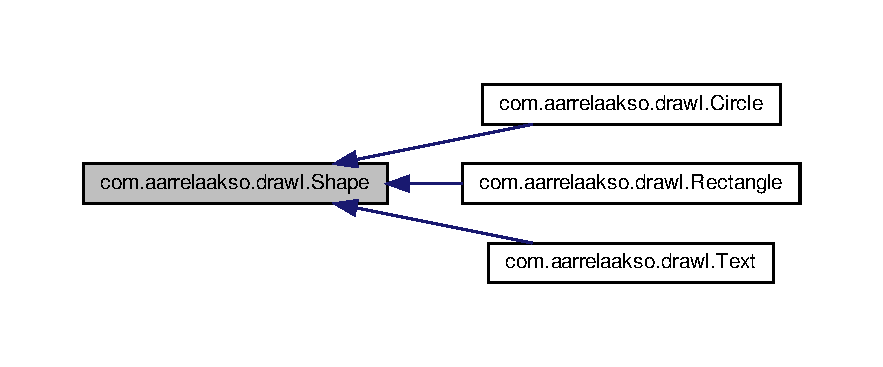
\includegraphics[width=350pt]{d1/d7f/classcom_1_1aarrelaakso_1_1drawl_1_1_shape__inherit__graph}
\end{center}
\end{figure}


Collaboration diagram for com.\+aarrelaakso.\+drawl.\+Shape\+:
\nopagebreak
\begin{figure}[H]
\begin{center}
\leavevmode
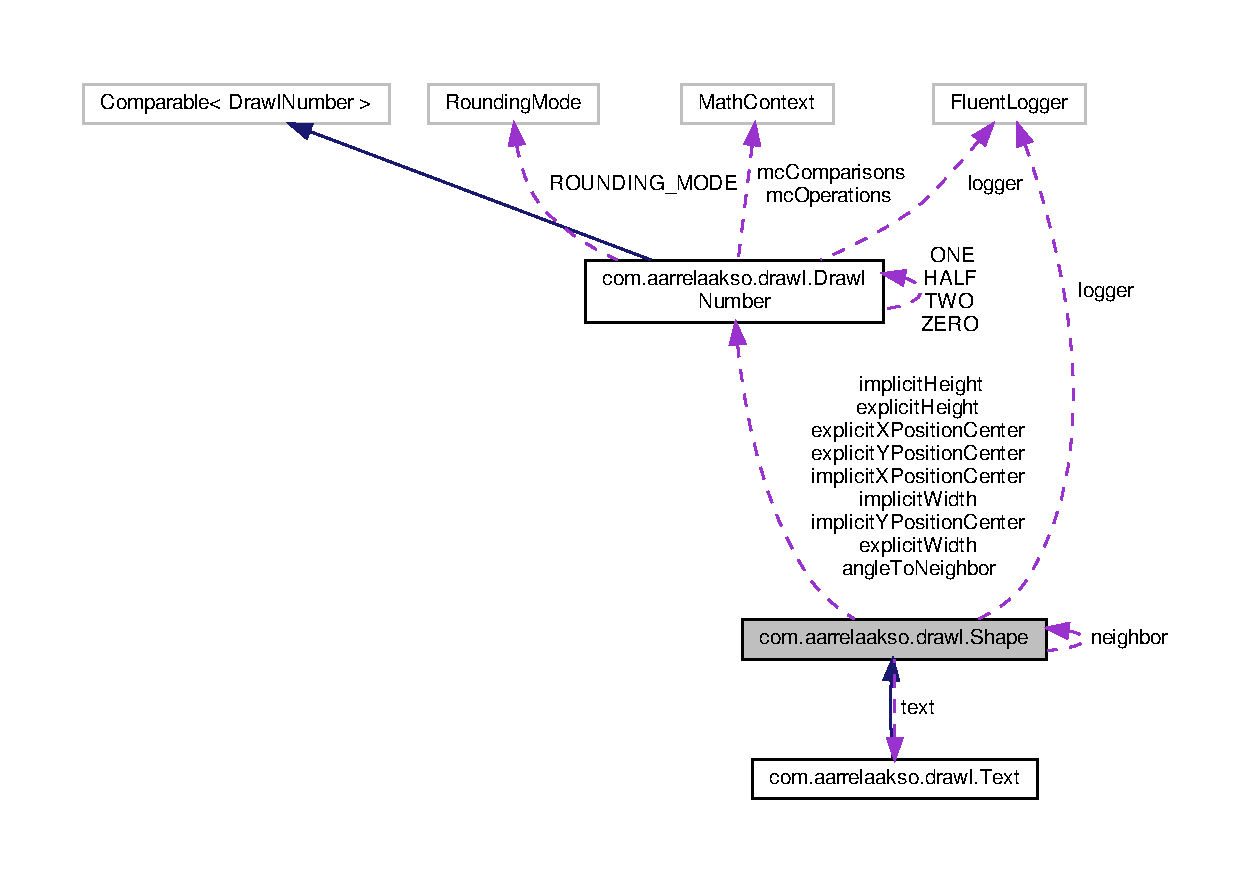
\includegraphics[width=350pt]{d7/d06/classcom_1_1aarrelaakso_1_1drawl_1_1_shape__coll__graph}
\end{center}
\end{figure}
\subsection*{Public Member Functions}
\begin{DoxyCompactItemize}
\item 
void \hyperlink{classcom_1_1aarrelaakso_1_1drawl_1_1_shape_af6fea9610721de462c18ee640043aba7}{add\+Text} (@Nullable final \hyperlink{classcom_1_1aarrelaakso_1_1drawl_1_1_text}{Text} \hyperlink{classcom_1_1aarrelaakso_1_1drawl_1_1_shape_ab54afc2d95d3447532f5ecf3fec3faa8}{text})
\begin{DoxyCompactList}\small\item\em Adds \hyperlink{classcom_1_1aarrelaakso_1_1drawl_1_1_text}{Text} inside this \hyperlink{classcom_1_1aarrelaakso_1_1drawl_1_1_shape}{Shape}. \end{DoxyCompactList}\item 
\hyperlink{classcom_1_1aarrelaakso_1_1drawl_1_1_shape}{Shape} \hyperlink{classcom_1_1aarrelaakso_1_1drawl_1_1_shape_acebea2aa57031322323c9bf50ee447db}{get\+Above} ()
\begin{DoxyCompactList}\small\item\em Gets this \hyperlink{classcom_1_1aarrelaakso_1_1drawl_1_1_shape}{Shape}\textquotesingle{}s neighbor above (this \hyperlink{classcom_1_1aarrelaakso_1_1drawl_1_1_shape}{Shape} is below that one), if any. \end{DoxyCompactList}\item 
void \hyperlink{classcom_1_1aarrelaakso_1_1drawl_1_1_shape_a4deb22d64fef2115a0bc4802e8dba682}{set\+Above} (@Not\+Null final \hyperlink{classcom_1_1aarrelaakso_1_1drawl_1_1_shape}{Shape} shape)
\begin{DoxyCompactList}\small\item\em Sets this \hyperlink{classcom_1_1aarrelaakso_1_1drawl_1_1_shape}{Shape} above another \hyperlink{classcom_1_1aarrelaakso_1_1drawl_1_1_shape}{Shape}. \end{DoxyCompactList}\item 
\hyperlink{classcom_1_1aarrelaakso_1_1drawl_1_1_shape}{Shape} \hyperlink{classcom_1_1aarrelaakso_1_1drawl_1_1_shape_a53de5ab609d879719cd3b372dfe8df58}{get\+Below} ()
\begin{DoxyCompactList}\small\item\em Gets this \hyperlink{classcom_1_1aarrelaakso_1_1drawl_1_1_shape}{Shape}\textquotesingle{}s neighbor below (this \hyperlink{classcom_1_1aarrelaakso_1_1drawl_1_1_shape}{Shape} is above that one), if any. \end{DoxyCompactList}\item 
void \hyperlink{classcom_1_1aarrelaakso_1_1drawl_1_1_shape_a4147526667449f5beb534d4404ba8f77}{set\+Below} (@Not\+Null final \hyperlink{classcom_1_1aarrelaakso_1_1drawl_1_1_shape}{Shape} shape)
\begin{DoxyCompactList}\small\item\em Sets this \hyperlink{classcom_1_1aarrelaakso_1_1drawl_1_1_shape}{Shape} below another \hyperlink{classcom_1_1aarrelaakso_1_1drawl_1_1_shape}{Shape}. \end{DoxyCompactList}\item 
\hyperlink{classcom_1_1aarrelaakso_1_1drawl_1_1_point}{Point} \hyperlink{classcom_1_1aarrelaakso_1_1drawl_1_1_shape_aba14efe9a16c0808580963c66b171082}{get\+Bottom\+Port} ()
\begin{DoxyCompactList}\small\item\em Returns a \hyperlink{classcom_1_1aarrelaakso_1_1drawl_1_1_point}{Point} object representing this \hyperlink{classcom_1_1aarrelaakso_1_1drawl_1_1_shape}{Shape}\textquotesingle{}s bottom port. \end{DoxyCompactList}\item 
String \hyperlink{classcom_1_1aarrelaakso_1_1drawl_1_1_shape_a0d9a33a3e151aaceeec140bea343a650}{get\+Fill} ()
\begin{DoxyCompactList}\small\item\em Returns the fill associated with this \hyperlink{classcom_1_1aarrelaakso_1_1drawl_1_1_shape}{Shape}, if any. \end{DoxyCompactList}\item 
void \hyperlink{classcom_1_1aarrelaakso_1_1drawl_1_1_shape_a81ff4feb49b8f74c1a639564748a23ee}{set\+Fill} (final String s)
\begin{DoxyCompactList}\small\item\em Set the fill of this \hyperlink{classcom_1_1aarrelaakso_1_1drawl_1_1_shape}{Shape}. \end{DoxyCompactList}\item 
\hyperlink{classcom_1_1aarrelaakso_1_1drawl_1_1_measure}{Measure} \hyperlink{classcom_1_1aarrelaakso_1_1drawl_1_1_shape_ac9f74d31c332aab76b329edc22080e67}{get\+Height} ()
\begin{DoxyCompactList}\small\item\em Returns a \hyperlink{classcom_1_1aarrelaakso_1_1drawl_1_1_measure}{Measure} object that represents the height of this \hyperlink{classcom_1_1aarrelaakso_1_1drawl_1_1_shape}{Shape}. \end{DoxyCompactList}\item 
\hyperlink{classcom_1_1aarrelaakso_1_1drawl_1_1_shape}{Shape} \hyperlink{classcom_1_1aarrelaakso_1_1drawl_1_1_shape_a2b19d5964ac46d545a7bae3133df6532}{get\+Left\+Of} ()
\begin{DoxyCompactList}\small\item\em Gets this \hyperlink{classcom_1_1aarrelaakso_1_1drawl_1_1_shape}{Shape}\textquotesingle{}s neighbor to the right (this \hyperlink{classcom_1_1aarrelaakso_1_1drawl_1_1_shape}{Shape} is to the left of that one), if any. \end{DoxyCompactList}\item 
void \hyperlink{classcom_1_1aarrelaakso_1_1drawl_1_1_shape_a0aef56392d76202235a9520394e87492}{set\+Left\+Of} (@Not\+Null final \hyperlink{classcom_1_1aarrelaakso_1_1drawl_1_1_shape}{Shape} shape)
\begin{DoxyCompactList}\small\item\em Sets this \hyperlink{classcom_1_1aarrelaakso_1_1drawl_1_1_shape}{Shape} to the left of another one. \end{DoxyCompactList}\item 
\hyperlink{classcom_1_1aarrelaakso_1_1drawl_1_1_point}{Point} \hyperlink{classcom_1_1aarrelaakso_1_1drawl_1_1_shape_aeffa96786ca552adf46924ec77da9555}{get\+Left\+Port} ()
\begin{DoxyCompactList}\small\item\em Returns a \hyperlink{classcom_1_1aarrelaakso_1_1drawl_1_1_point}{Point} object representing this \hyperlink{classcom_1_1aarrelaakso_1_1drawl_1_1_shape}{Shape}\textquotesingle{}s left port. \end{DoxyCompactList}\item 
\hyperlink{classcom_1_1aarrelaakso_1_1drawl_1_1_shape}{Shape} \hyperlink{classcom_1_1aarrelaakso_1_1drawl_1_1_shape_a1ad573b06f341aa79f6a255a476ae6e4}{get\+Right\+Of} ()
\begin{DoxyCompactList}\small\item\em Gets this \hyperlink{classcom_1_1aarrelaakso_1_1drawl_1_1_shape}{Shape}\textquotesingle{}s neighbor to the left (this \hyperlink{classcom_1_1aarrelaakso_1_1drawl_1_1_shape}{Shape} is to the right of that one), if any. \end{DoxyCompactList}\item 
void \hyperlink{classcom_1_1aarrelaakso_1_1drawl_1_1_shape_a3cada5e03bd1552a79702d2945c7ed01}{set\+Right\+Of} (@Not\+Null final \hyperlink{classcom_1_1aarrelaakso_1_1drawl_1_1_shape}{Shape} shape)
\begin{DoxyCompactList}\small\item\em Sets this \hyperlink{classcom_1_1aarrelaakso_1_1drawl_1_1_shape}{Shape}\textquotesingle{}s neighbor to the left (this \hyperlink{classcom_1_1aarrelaakso_1_1drawl_1_1_shape}{Shape} is to the right of that one). \end{DoxyCompactList}\item 
\hyperlink{classcom_1_1aarrelaakso_1_1drawl_1_1_point}{Point} \hyperlink{classcom_1_1aarrelaakso_1_1drawl_1_1_shape_a319c78d425ec91e1aef1072a95e349ad}{get\+Right\+Port} ()
\begin{DoxyCompactList}\small\item\em Returns a \hyperlink{classcom_1_1aarrelaakso_1_1drawl_1_1_point}{Point} object representing this \hyperlink{classcom_1_1aarrelaakso_1_1drawl_1_1_shape}{Shape}\textquotesingle{}s left port. \end{DoxyCompactList}\item 
String \hyperlink{classcom_1_1aarrelaakso_1_1drawl_1_1_shape_aca74cc0c71117040f28329744eebde9d}{get\+S\+VG} ()
\item 
String \hyperlink{classcom_1_1aarrelaakso_1_1drawl_1_1_shape_a4e1d54c7e161e3af5053939ddefdf9e6}{get\+Stroke} ()
\begin{DoxyCompactList}\small\item\em Gets the stroke of this \hyperlink{classcom_1_1aarrelaakso_1_1drawl_1_1_shape}{Shape}. \end{DoxyCompactList}\item 
void \hyperlink{classcom_1_1aarrelaakso_1_1drawl_1_1_shape_a75685cbfea36858836df8e1fb4f8b821}{set\+Stroke} (final String s)
\begin{DoxyCompactList}\small\item\em Sets the stroke of this shape. \end{DoxyCompactList}\item 
\hyperlink{classcom_1_1aarrelaakso_1_1drawl_1_1_text}{Text} \hyperlink{classcom_1_1aarrelaakso_1_1drawl_1_1_shape_a6f876978d4102974fedc5b41c93c7b26}{get\+Text} ()
\begin{DoxyCompactList}\small\item\em Returns a \hyperlink{classcom_1_1aarrelaakso_1_1drawl_1_1_text}{Text} object that belongs to this \hyperlink{classcom_1_1aarrelaakso_1_1drawl_1_1_shape}{Shape}, if there is one. \end{DoxyCompactList}\item 
\hyperlink{classcom_1_1aarrelaakso_1_1drawl_1_1_point}{Point} \hyperlink{classcom_1_1aarrelaakso_1_1drawl_1_1_shape_aed4e9caa294aacc973b7a531a960e9e5}{get\+Top\+Port} ()
\begin{DoxyCompactList}\small\item\em Returns a \hyperlink{classcom_1_1aarrelaakso_1_1drawl_1_1_point}{Point} object representing this \hyperlink{classcom_1_1aarrelaakso_1_1drawl_1_1_shape}{Shape}\textquotesingle{}s top port. \end{DoxyCompactList}\item 
\hyperlink{classcom_1_1aarrelaakso_1_1drawl_1_1_measure}{Measure} \hyperlink{classcom_1_1aarrelaakso_1_1drawl_1_1_shape_a3e2c58984f1bcbc2e9e86cf30868561e}{get\+Width} ()
\begin{DoxyCompactList}\small\item\em Returns a \hyperlink{classcom_1_1aarrelaakso_1_1drawl_1_1_measure}{Measure} object that represents the width of this \hyperlink{classcom_1_1aarrelaakso_1_1drawl_1_1_shape}{Shape}. \end{DoxyCompactList}\item 
Boolean \hyperlink{classcom_1_1aarrelaakso_1_1drawl_1_1_shape_a037a5515b2a6e1df1d1981aa5516e78e}{has\+Text} ()
\begin{DoxyCompactList}\small\item\em Indicates whether this shape has a \hyperlink{classcom_1_1aarrelaakso_1_1drawl_1_1_text}{Text} object associated with it. \end{DoxyCompactList}\item 
void \hyperlink{classcom_1_1aarrelaakso_1_1drawl_1_1_shape_aad0b2fb173c0112b71b06cf90709acc3}{set\+Above} (@Not\+Null final \hyperlink{classcom_1_1aarrelaakso_1_1drawl_1_1_shape}{Shape} shape, @Not\+Null final \hyperlink{classcom_1_1aarrelaakso_1_1drawl_1_1_measure}{Measure} offset)
\begin{DoxyCompactList}\small\item\em Sets this \hyperlink{classcom_1_1aarrelaakso_1_1drawl_1_1_shape}{Shape} above another \hyperlink{classcom_1_1aarrelaakso_1_1drawl_1_1_shape}{Shape}. \end{DoxyCompactList}\item 
void \hyperlink{classcom_1_1aarrelaakso_1_1drawl_1_1_shape_a63c902c4e79235901744c6d83544fa54}{set\+Below} (@Not\+Null final \hyperlink{classcom_1_1aarrelaakso_1_1drawl_1_1_shape}{Shape} shape, @Not\+Null final \hyperlink{classcom_1_1aarrelaakso_1_1drawl_1_1_measure}{Measure} offset)
\begin{DoxyCompactList}\small\item\em Sets this circle below another circle. \end{DoxyCompactList}\item 
void \hyperlink{classcom_1_1aarrelaakso_1_1drawl_1_1_shape_a8012a3823982d77b563ef61787ccb523}{set\+Left\+Of} (@Not\+Null final \hyperlink{classcom_1_1aarrelaakso_1_1drawl_1_1_shape}{Shape} shape, @Not\+Null final \hyperlink{classcom_1_1aarrelaakso_1_1drawl_1_1_measure}{Measure} offset)
\begin{DoxyCompactList}\small\item\em Sets this \hyperlink{classcom_1_1aarrelaakso_1_1drawl_1_1_shape}{Shape}\textquotesingle{}s neighbor to the right (this \hyperlink{classcom_1_1aarrelaakso_1_1drawl_1_1_shape}{Shape} is to the left of that one). \end{DoxyCompactList}\item 
void \hyperlink{classcom_1_1aarrelaakso_1_1drawl_1_1_shape_a89e85848d24dca0fa60ff68d169eef11}{set\+Right\+Of} (@Not\+Null final \hyperlink{classcom_1_1aarrelaakso_1_1drawl_1_1_shape}{Shape} shape, @Not\+Null final \hyperlink{classcom_1_1aarrelaakso_1_1drawl_1_1_measure}{Measure} offset)
\begin{DoxyCompactList}\small\item\em Sets this \hyperlink{classcom_1_1aarrelaakso_1_1drawl_1_1_shape}{Shape}\textquotesingle{}s neighbor to the left with an offset. \end{DoxyCompactList}\end{DoxyCompactItemize}
\subsection*{Protected Member Functions}
\begin{DoxyCompactItemize}
\item 
\hyperlink{interfacecom_1_1aarrelaakso_1_1drawl_1_1_number}{Number} \hyperlink{classcom_1_1aarrelaakso_1_1drawl_1_1_shape_a3acdc2fd1944e2efacd0bfbb8aefe89b}{get\+Explicit\+Half\+Width} ()
\begin{DoxyCompactList}\small\item\em Gets half the explicit width of this \hyperlink{classcom_1_1aarrelaakso_1_1drawl_1_1_shape}{Shape}. \end{DoxyCompactList}\item 
\hyperlink{interfacecom_1_1aarrelaakso_1_1drawl_1_1_number}{Number} \hyperlink{classcom_1_1aarrelaakso_1_1drawl_1_1_shape_a48917787cedbfd447cd37edbb59a1145}{get\+Explicit\+Height} ()
\begin{DoxyCompactList}\small\item\em Get the explicit height of this \hyperlink{classcom_1_1aarrelaakso_1_1drawl_1_1_shape}{Shape}. \end{DoxyCompactList}\item 
void \hyperlink{classcom_1_1aarrelaakso_1_1drawl_1_1_shape_a3680a63cef0d766132d1f64813ca8eca}{set\+Explicit\+Height} (@Nullable final \hyperlink{interfacecom_1_1aarrelaakso_1_1drawl_1_1_number}{Number} height)
\begin{DoxyCompactList}\small\item\em Set the height of this \hyperlink{classcom_1_1aarrelaakso_1_1drawl_1_1_shape}{Shape} to an explicit value. \end{DoxyCompactList}\item 
\hyperlink{interfacecom_1_1aarrelaakso_1_1drawl_1_1_number}{Number} \hyperlink{classcom_1_1aarrelaakso_1_1drawl_1_1_shape_aca08f18bbe102a5cf6a77cb746d42875}{get\+Explicit\+Width} ()
\begin{DoxyCompactList}\small\item\em Get the explicit width of this \hyperlink{classcom_1_1aarrelaakso_1_1drawl_1_1_shape}{Shape}. \end{DoxyCompactList}\item 
void \hyperlink{classcom_1_1aarrelaakso_1_1drawl_1_1_shape_a386685477bfc007aab782565f140265d}{set\+Explicit\+Width} (@Nullable final \hyperlink{interfacecom_1_1aarrelaakso_1_1drawl_1_1_number}{Number} width)
\begin{DoxyCompactList}\small\item\em Set the width of this \hyperlink{classcom_1_1aarrelaakso_1_1drawl_1_1_shape}{Shape} to an explicit value. \end{DoxyCompactList}\item 
\hyperlink{interfacecom_1_1aarrelaakso_1_1drawl_1_1_number}{Number} \hyperlink{classcom_1_1aarrelaakso_1_1drawl_1_1_shape_aa1fbd5a290bc5d2df437f0bd79f30a89}{get\+Explicit\+X\+Position\+Center} ()
\begin{DoxyCompactList}\small\item\em Gets the explicit x-\/position of the center of this \hyperlink{classcom_1_1aarrelaakso_1_1drawl_1_1_shape}{Shape}. \end{DoxyCompactList}\item 
void \hyperlink{classcom_1_1aarrelaakso_1_1drawl_1_1_shape_a28c766b414be0cd8767093f9be557dbd}{set\+Explicit\+X\+Position\+Center} (final \hyperlink{interfacecom_1_1aarrelaakso_1_1drawl_1_1_number}{Number} x)
\begin{DoxyCompactList}\small\item\em Sets the explicit center position of this \hyperlink{classcom_1_1aarrelaakso_1_1drawl_1_1_shape}{Shape}. \end{DoxyCompactList}\item 
void \hyperlink{classcom_1_1aarrelaakso_1_1drawl_1_1_shape_a271cd9377952616a30a434b22e22000a}{set\+Explicit\+X\+Position\+Center} (final Integer x)
\begin{DoxyCompactList}\small\item\em Sets the explicit x position of the center of this \hyperlink{classcom_1_1aarrelaakso_1_1drawl_1_1_shape}{Shape}. \end{DoxyCompactList}\item 
\hyperlink{interfacecom_1_1aarrelaakso_1_1drawl_1_1_number}{Number} \hyperlink{classcom_1_1aarrelaakso_1_1drawl_1_1_shape_abd7f6c77e2c62100bb72d8ad3085e288}{get\+Explicit\+X\+Position\+Left} ()
\begin{DoxyCompactList}\small\item\em Gets the explicit x position of the left edge of this \hyperlink{classcom_1_1aarrelaakso_1_1drawl_1_1_shape}{Shape}. \end{DoxyCompactList}\item 
\hyperlink{interfacecom_1_1aarrelaakso_1_1drawl_1_1_number}{Number} \hyperlink{classcom_1_1aarrelaakso_1_1drawl_1_1_shape_a86920ba43a76d5a02977e5f9ea3509ac}{get\+Explicit\+X\+Position\+Right} ()
\begin{DoxyCompactList}\small\item\em Gets the explicit x position of the right edge of this \hyperlink{classcom_1_1aarrelaakso_1_1drawl_1_1_shape}{Shape}. \end{DoxyCompactList}\item 
\hyperlink{interfacecom_1_1aarrelaakso_1_1drawl_1_1_number}{Number} \hyperlink{classcom_1_1aarrelaakso_1_1drawl_1_1_shape_a28b8e03381be6afdc7c5c8da48c80afe}{get\+Explicit\+Y\+Position\+Bottom} ()
\begin{DoxyCompactList}\small\item\em Gets the explicit y position of the bottom of this \hyperlink{classcom_1_1aarrelaakso_1_1drawl_1_1_shape}{Shape}. \end{DoxyCompactList}\item 
\hyperlink{interfacecom_1_1aarrelaakso_1_1drawl_1_1_number}{Number} \hyperlink{classcom_1_1aarrelaakso_1_1drawl_1_1_shape_a1e46cc626d5f5e1360d9d35d23cc50ea}{get\+Explicit\+Y\+Position\+Center} ()
\begin{DoxyCompactList}\small\item\em Gets the explicit y-\/position of the center of this \hyperlink{classcom_1_1aarrelaakso_1_1drawl_1_1_shape}{Shape}. \end{DoxyCompactList}\item 
void \hyperlink{classcom_1_1aarrelaakso_1_1drawl_1_1_shape_a93e9e1bdd05f111661660e9de621cd12}{set\+Explicit\+Y\+Position\+Center} (final Integer y)
\begin{DoxyCompactList}\small\item\em Sets the explicit y-\/position of the center of this \hyperlink{classcom_1_1aarrelaakso_1_1drawl_1_1_shape}{Shape}. \end{DoxyCompactList}\item 
void \hyperlink{classcom_1_1aarrelaakso_1_1drawl_1_1_shape_a7d49d69bd74e57c3a3341a025c3cce50}{set\+Explicit\+Y\+Position\+Center} (final \hyperlink{interfacecom_1_1aarrelaakso_1_1drawl_1_1_number}{Number} y)
\begin{DoxyCompactList}\small\item\em Sets the explicit y position of this \hyperlink{classcom_1_1aarrelaakso_1_1drawl_1_1_shape}{Shape}. \end{DoxyCompactList}\item 
\hyperlink{interfacecom_1_1aarrelaakso_1_1drawl_1_1_number}{Number} \hyperlink{classcom_1_1aarrelaakso_1_1drawl_1_1_shape_a8c65dff2026744ae10648de3908165e5}{get\+Explicit\+Y\+Position\+Top} ()
\begin{DoxyCompactList}\small\item\em Gets the explicit y-\/position of the top of this \hyperlink{classcom_1_1aarrelaakso_1_1drawl_1_1_shape}{Shape}. \end{DoxyCompactList}\item 
\hyperlink{interfacecom_1_1aarrelaakso_1_1drawl_1_1_number}{Number} \hyperlink{classcom_1_1aarrelaakso_1_1drawl_1_1_shape_a4af0fd7e309ea01bced73076510ef897}{get\+Implicit\+Half\+Height} ()
\begin{DoxyCompactList}\small\item\em Gets half of the implicit height of this \hyperlink{classcom_1_1aarrelaakso_1_1drawl_1_1_shape}{Shape}. \end{DoxyCompactList}\item 
\hyperlink{interfacecom_1_1aarrelaakso_1_1drawl_1_1_number}{Number} \hyperlink{classcom_1_1aarrelaakso_1_1drawl_1_1_shape_a02d73887a309bcd1178b142ad0c7edd9}{get\+Implicit\+Half\+Width} ()
\begin{DoxyCompactList}\small\item\em Gets half of the implicit width of this \hyperlink{classcom_1_1aarrelaakso_1_1drawl_1_1_shape}{Shape}. \end{DoxyCompactList}\item 
\hyperlink{interfacecom_1_1aarrelaakso_1_1drawl_1_1_number}{Number} \hyperlink{classcom_1_1aarrelaakso_1_1drawl_1_1_shape_a3b0ad73b41fe8c9ae66d20f7fc1de7c9}{get\+Implicit\+Height} ()
\begin{DoxyCompactList}\small\item\em Gets the implicit height of this \hyperlink{classcom_1_1aarrelaakso_1_1drawl_1_1_shape}{Shape}. \end{DoxyCompactList}\item 
final void \hyperlink{classcom_1_1aarrelaakso_1_1drawl_1_1_shape_a608e72be0fb16380e5fda14564c46739}{set\+Implicit\+Height} (@Not\+Null final \hyperlink{interfacecom_1_1aarrelaakso_1_1drawl_1_1_number}{Number} \hyperlink{classcom_1_1aarrelaakso_1_1drawl_1_1_shape_a9270317569c41e7f3f3fbe6e71df86e6}{implicit\+Height})
\begin{DoxyCompactList}\small\item\em Sets the implicit height of this \hyperlink{classcom_1_1aarrelaakso_1_1drawl_1_1_shape}{Shape}. \end{DoxyCompactList}\item 
\hyperlink{interfacecom_1_1aarrelaakso_1_1drawl_1_1_number}{Number} \hyperlink{classcom_1_1aarrelaakso_1_1drawl_1_1_shape_af8182545b3b1c85ecaee849474f63c6b}{get\+Implicit\+Width} ()
\begin{DoxyCompactList}\small\item\em Gets the implicit width of this \hyperlink{classcom_1_1aarrelaakso_1_1drawl_1_1_shape}{Shape}. \end{DoxyCompactList}\item 
final void \hyperlink{classcom_1_1aarrelaakso_1_1drawl_1_1_shape_acc3e365064b5d4f719ac920a5a70aedb}{set\+Implicit\+Width} (@Not\+Null final \hyperlink{interfacecom_1_1aarrelaakso_1_1drawl_1_1_number}{Number} \hyperlink{classcom_1_1aarrelaakso_1_1drawl_1_1_shape_a06c9063aa0b51139910e23414428c9d6}{implicit\+Width})
\begin{DoxyCompactList}\small\item\em Sets the implicit width of this \hyperlink{classcom_1_1aarrelaakso_1_1drawl_1_1_shape}{Shape}. \end{DoxyCompactList}\item 
\hyperlink{interfacecom_1_1aarrelaakso_1_1drawl_1_1_number}{Number} \hyperlink{classcom_1_1aarrelaakso_1_1drawl_1_1_shape_a0903079fd35e3cfdd6cdc299548a9680}{get\+Implicit\+X\+Maximum} ()
\begin{DoxyCompactList}\small\item\em Get the implicit maximum (rightmost) x-\/position of this \hyperlink{classcom_1_1aarrelaakso_1_1drawl_1_1_shape}{Shape}. \end{DoxyCompactList}\item 
\hyperlink{interfacecom_1_1aarrelaakso_1_1drawl_1_1_number}{Number} \hyperlink{classcom_1_1aarrelaakso_1_1drawl_1_1_shape_a264da8a94218b09267c2e177ff0b0951}{get\+Implicit\+X\+Minimum} ()
\begin{DoxyCompactList}\small\item\em Get the implicit minimum (leftmost) x-\/position of this \hyperlink{classcom_1_1aarrelaakso_1_1drawl_1_1_shape}{Shape}. \end{DoxyCompactList}\item 
\hyperlink{interfacecom_1_1aarrelaakso_1_1drawl_1_1_number}{Number} \hyperlink{classcom_1_1aarrelaakso_1_1drawl_1_1_shape_a9632097be62eb03e09145763852bda85}{get\+Implicit\+X\+Position\+Center} ()
\begin{DoxyCompactList}\small\item\em Get the implicit x position of the center of this \hyperlink{classcom_1_1aarrelaakso_1_1drawl_1_1_shape}{Shape}. \end{DoxyCompactList}\item 
void \hyperlink{classcom_1_1aarrelaakso_1_1drawl_1_1_shape_a945597709a9d79688e48a9802c86b13b}{set\+Implicit\+X\+Position\+Center} (final \hyperlink{interfacecom_1_1aarrelaakso_1_1drawl_1_1_number}{Number} x)
\begin{DoxyCompactList}\small\item\em Sets the implicit x position of the center of this \hyperlink{classcom_1_1aarrelaakso_1_1drawl_1_1_shape}{Shape}. \end{DoxyCompactList}\item 
\hyperlink{interfacecom_1_1aarrelaakso_1_1drawl_1_1_number}{Number} \hyperlink{classcom_1_1aarrelaakso_1_1drawl_1_1_shape_a2f272e8bfa625bb7959d1f722d5ac3df}{get\+Implicit\+X\+Position\+Left} ()
\begin{DoxyCompactList}\small\item\em Gets the implicit x position of the left edge of this \hyperlink{classcom_1_1aarrelaakso_1_1drawl_1_1_shape}{Shape}. \end{DoxyCompactList}\item 
\hyperlink{interfacecom_1_1aarrelaakso_1_1drawl_1_1_number}{Number} \hyperlink{classcom_1_1aarrelaakso_1_1drawl_1_1_shape_a15599ef4ee30a0ddd372f7cf1b155ce1}{get\+Implicit\+X\+Position\+Right} ()
\begin{DoxyCompactList}\small\item\em Gets the implicit x position of the right edge of this \hyperlink{classcom_1_1aarrelaakso_1_1drawl_1_1_shape}{Shape}. \end{DoxyCompactList}\item 
\hyperlink{interfacecom_1_1aarrelaakso_1_1drawl_1_1_number}{Number} \hyperlink{classcom_1_1aarrelaakso_1_1drawl_1_1_shape_a8d44b02976656bf4a81055a2dbae66cb}{get\+Implicit\+Y\+Position\+Bottom} ()
\begin{DoxyCompactList}\small\item\em Gets the implicit bottommost y-\/position of this \hyperlink{classcom_1_1aarrelaakso_1_1drawl_1_1_shape}{Shape}. \end{DoxyCompactList}\item 
\hyperlink{interfacecom_1_1aarrelaakso_1_1drawl_1_1_number}{Number} \hyperlink{classcom_1_1aarrelaakso_1_1drawl_1_1_shape_a1f27f0adc1716dc60691a7d0c14f2ace}{get\+Implicit\+Y\+Position\+Center} ()
\begin{DoxyCompactList}\small\item\em Gets the implicit y position of the center of this \hyperlink{classcom_1_1aarrelaakso_1_1drawl_1_1_shape}{Shape}. \end{DoxyCompactList}\item 
void \hyperlink{classcom_1_1aarrelaakso_1_1drawl_1_1_shape_a79c79420c626b8b2d2534b6c9aa64d8f}{set\+Implicit\+Y\+Position\+Center} (final \hyperlink{interfacecom_1_1aarrelaakso_1_1drawl_1_1_number}{Number} y)
\begin{DoxyCompactList}\small\item\em Sets the implicit y position of this \hyperlink{classcom_1_1aarrelaakso_1_1drawl_1_1_shape}{Shape}. \end{DoxyCompactList}\item 
\hyperlink{interfacecom_1_1aarrelaakso_1_1drawl_1_1_number}{Number} \hyperlink{classcom_1_1aarrelaakso_1_1drawl_1_1_shape_a6a52176302dd9b5d2bfc2d25409c310e}{get\+Implicit\+Y\+Position\+Top} ()
\begin{DoxyCompactList}\small\item\em Gets the implicit topmost y position of this \hyperlink{classcom_1_1aarrelaakso_1_1drawl_1_1_shape}{Shape}. \end{DoxyCompactList}\end{DoxyCompactItemize}
\subsection*{Static Package Functions}
\begin{DoxyCompactItemize}
\item 
\hyperlink{classcom_1_1aarrelaakso_1_1drawl_1_1_shape_ad2adcb85374cf5d6d59429628314e8d1}{\mbox{[}static initializer\mbox{]}}
\end{DoxyCompactItemize}
\subsection*{Private Member Functions}
\begin{DoxyCompactItemize}
\item 
\hyperlink{interfacecom_1_1aarrelaakso_1_1drawl_1_1_number}{Number} \hyperlink{classcom_1_1aarrelaakso_1_1drawl_1_1_shape_a10833aa0e7e8ef7b45c866ccf6d419e5}{get\+Explicit\+Half\+Height} ()
\begin{DoxyCompactList}\small\item\em Gets half the explicit height of this \hyperlink{classcom_1_1aarrelaakso_1_1drawl_1_1_shape}{Shape}. \end{DoxyCompactList}\end{DoxyCompactItemize}
\subsection*{Private Attributes}
\begin{DoxyCompactItemize}
\item 
\hyperlink{interfacecom_1_1aarrelaakso_1_1drawl_1_1_number}{Number} \hyperlink{classcom_1_1aarrelaakso_1_1drawl_1_1_shape_a0281d9f3d35d7ff5db2be3c3f9362c9f}{angle\+To\+Neighbor}
\begin{DoxyCompactList}\small\item\em The angle, in degrees, to a neighbor. \end{DoxyCompactList}\item 
\hyperlink{interfacecom_1_1aarrelaakso_1_1drawl_1_1_number}{Number} \hyperlink{classcom_1_1aarrelaakso_1_1drawl_1_1_shape_aa153ceaedb47e7aa504cd52a556dc7ac}{explicit\+Height}
\begin{DoxyCompactList}\small\item\em The explicit height of a \hyperlink{classcom_1_1aarrelaakso_1_1drawl_1_1_shape}{Shape} defaults to {\ttfamily null} to indicate it that has not yet been set. \end{DoxyCompactList}\item 
\hyperlink{interfacecom_1_1aarrelaakso_1_1drawl_1_1_number}{Number} \hyperlink{classcom_1_1aarrelaakso_1_1drawl_1_1_shape_af297289dcb30e099587976e95431e327}{explicit\+Width}
\begin{DoxyCompactList}\small\item\em The explicit width of a \hyperlink{classcom_1_1aarrelaakso_1_1drawl_1_1_shape}{Shape} defaults to {\ttfamily null} to indicate that it has not yet been set. \end{DoxyCompactList}\item 
\hyperlink{classcom_1_1aarrelaakso_1_1drawl_1_1_point}{Point} \hyperlink{classcom_1_1aarrelaakso_1_1drawl_1_1_shape_ab843843602722cca47778675d5d77bb5}{explicit\+Position\+Center} = new \hyperlink{classcom_1_1aarrelaakso_1_1drawl_1_1_point}{Point}(0, 0)
\begin{DoxyCompactList}\small\item\em A default \hyperlink{classcom_1_1aarrelaakso_1_1drawl_1_1_shape}{Shape} is centered at (0,0) in explicit coordinates. \end{DoxyCompactList}\item 
String \hyperlink{classcom_1_1aarrelaakso_1_1drawl_1_1_shape_ade398fbc41c7814eebb5b4c7a62861f6}{fill}
\begin{DoxyCompactList}\small\item\em The fill of this \hyperlink{classcom_1_1aarrelaakso_1_1drawl_1_1_shape}{Shape}. \end{DoxyCompactList}\item 
\hyperlink{interfacecom_1_1aarrelaakso_1_1drawl_1_1_number}{Number} \hyperlink{classcom_1_1aarrelaakso_1_1drawl_1_1_shape_a9270317569c41e7f3f3fbe6e71df86e6}{implicit\+Height} = \hyperlink{classcom_1_1aarrelaakso_1_1drawl_1_1_drawl_number_a0cd06e1d6344869ed300bc99afcde20a}{Drawl\+Number.\+O\+NE}
\begin{DoxyCompactList}\small\item\em The implicit height of a default \hyperlink{classcom_1_1aarrelaakso_1_1drawl_1_1_shape}{Shape} is 1. \end{DoxyCompactList}\item 
\hyperlink{interfacecom_1_1aarrelaakso_1_1drawl_1_1_number}{Number} \hyperlink{classcom_1_1aarrelaakso_1_1drawl_1_1_shape_a06c9063aa0b51139910e23414428c9d6}{implicit\+Width} = \hyperlink{classcom_1_1aarrelaakso_1_1drawl_1_1_drawl_number_a0cd06e1d6344869ed300bc99afcde20a}{Drawl\+Number.\+O\+NE}
\begin{DoxyCompactList}\small\item\em The implicit width of a default \hyperlink{classcom_1_1aarrelaakso_1_1drawl_1_1_shape}{Shape} is 1. \end{DoxyCompactList}\item 
\hyperlink{classcom_1_1aarrelaakso_1_1drawl_1_1_point}{Point} \hyperlink{classcom_1_1aarrelaakso_1_1drawl_1_1_shape_af3b507f99acaa3b6b28f1e2e91409e1e}{implicit\+Position\+Center} = new \hyperlink{classcom_1_1aarrelaakso_1_1drawl_1_1_point}{Point}(0, 0)
\begin{DoxyCompactList}\small\item\em A default \hyperlink{classcom_1_1aarrelaakso_1_1drawl_1_1_shape}{Shape} is centered at (0,0) in implicit coordinates. \end{DoxyCompactList}\item 
\hyperlink{classcom_1_1aarrelaakso_1_1drawl_1_1_shape}{Shape} \hyperlink{classcom_1_1aarrelaakso_1_1drawl_1_1_shape_a57da030925a9bfc11bc49333b63a2e0f}{neighbor}
\begin{DoxyCompactList}\small\item\em A shape adjacent to this one, if any. \end{DoxyCompactList}\item 
String \hyperlink{classcom_1_1aarrelaakso_1_1drawl_1_1_shape_a7889c6cd8d073a3adad5ce6bcf8247a3}{stroke}
\begin{DoxyCompactList}\small\item\em The stroke of this \hyperlink{classcom_1_1aarrelaakso_1_1drawl_1_1_shape}{Shape}. \end{DoxyCompactList}\item 
\hyperlink{classcom_1_1aarrelaakso_1_1drawl_1_1_text}{Text} \hyperlink{classcom_1_1aarrelaakso_1_1drawl_1_1_shape_ab54afc2d95d3447532f5ecf3fec3faa8}{text}
\begin{DoxyCompactList}\small\item\em \hyperlink{classcom_1_1aarrelaakso_1_1drawl_1_1_text}{Text} inside this \hyperlink{classcom_1_1aarrelaakso_1_1drawl_1_1_shape}{Shape}. \end{DoxyCompactList}\end{DoxyCompactItemize}
\subsection*{Static Private Attributes}
\begin{DoxyCompactItemize}
\item 
static final \hyperlink{interfacecom_1_1aarrelaakso_1_1drawl_1_1_number}{Number} \hyperlink{classcom_1_1aarrelaakso_1_1drawl_1_1_shape_ac71780529ecfc46ae126d895d7735ac4}{A\+B\+O\+VE} = \hyperlink{classcom_1_1aarrelaakso_1_1drawl_1_1_drawl_number_ae79e88954ed30a7f939cc62836fdc75c}{Drawl\+Number.\+Z\+E\+RO}
\item 
static final \hyperlink{interfacecom_1_1aarrelaakso_1_1drawl_1_1_number}{Number} \hyperlink{classcom_1_1aarrelaakso_1_1drawl_1_1_shape_af670d34e6a0155ea0c350312d8ebc39f}{B\+E\+L\+OW} = \hyperlink{classcom_1_1aarrelaakso_1_1drawl_1_1_drawl_number_a368da87af7b1b38bd5185715afadcad6}{Drawl\+Number.\+value\+Of}(180)
\item 
static final \hyperlink{interfacecom_1_1aarrelaakso_1_1drawl_1_1_number}{Number} \hyperlink{classcom_1_1aarrelaakso_1_1drawl_1_1_shape_a682479373a5944ae84fc33fd65324e9d}{L\+E\+FT} = \hyperlink{classcom_1_1aarrelaakso_1_1drawl_1_1_drawl_number_a368da87af7b1b38bd5185715afadcad6}{Drawl\+Number.\+value\+Of}(270)
\item 
static final \hyperlink{interfacecom_1_1aarrelaakso_1_1drawl_1_1_number}{Number} \hyperlink{classcom_1_1aarrelaakso_1_1drawl_1_1_shape_ad4f620afc88ad5d6fadc698f443cbe38}{R\+I\+G\+HT} = \hyperlink{classcom_1_1aarrelaakso_1_1drawl_1_1_drawl_number_a368da87af7b1b38bd5185715afadcad6}{Drawl\+Number.\+value\+Of}(90)
\item 
static final String \hyperlink{classcom_1_1aarrelaakso_1_1drawl_1_1_shape_a82d5613ad2795e107346a68e48ae8379}{C\+A\+N\+N\+O\+T\+\_\+\+B\+E\+\_\+\+A\+D\+J\+A\+C\+E\+N\+T\+\_\+\+T\+O\+\_\+\+I\+T\+S\+E\+LF} = \char`\"{}A circle cannot be adjacent to itself\char`\"{}
\item 
static final Fluent\+Logger \hyperlink{classcom_1_1aarrelaakso_1_1drawl_1_1_shape_ab9ce64789a45acc1bdd2cee046264ff6}{logger}
\end{DoxyCompactItemize}


\subsection{Detailed Description}
Abstract class represents shapes such as circles, rectangles, and lines. 

\subsection{Member Function Documentation}
\mbox{\Hypertarget{classcom_1_1aarrelaakso_1_1drawl_1_1_shape_ad2adcb85374cf5d6d59429628314e8d1}\label{classcom_1_1aarrelaakso_1_1drawl_1_1_shape_ad2adcb85374cf5d6d59429628314e8d1}} 
\index{com\+::aarrelaakso\+::drawl\+::\+Shape@{com\+::aarrelaakso\+::drawl\+::\+Shape}!\mbox{[}static initializer\mbox{]}@{[static initializer]}}
\index{\mbox{[}static initializer\mbox{]}@{[static initializer]}!com\+::aarrelaakso\+::drawl\+::\+Shape@{com\+::aarrelaakso\+::drawl\+::\+Shape}}
\subsubsection{\texorpdfstring{[static initializer]()}{[static initializer]()}}
{\footnotesize\ttfamily com.\+aarrelaakso.\+drawl.\+Shape.\mbox{[}static initializer\mbox{]} (\begin{DoxyParamCaption}{ }\end{DoxyParamCaption})\hspace{0.3cm}{\ttfamily [static]}, {\ttfamily [package]}}

\mbox{\Hypertarget{classcom_1_1aarrelaakso_1_1drawl_1_1_shape_af6fea9610721de462c18ee640043aba7}\label{classcom_1_1aarrelaakso_1_1drawl_1_1_shape_af6fea9610721de462c18ee640043aba7}} 
\index{com\+::aarrelaakso\+::drawl\+::\+Shape@{com\+::aarrelaakso\+::drawl\+::\+Shape}!add\+Text@{add\+Text}}
\index{add\+Text@{add\+Text}!com\+::aarrelaakso\+::drawl\+::\+Shape@{com\+::aarrelaakso\+::drawl\+::\+Shape}}
\subsubsection{\texorpdfstring{add\+Text()}{addText()}}
{\footnotesize\ttfamily void com.\+aarrelaakso.\+drawl.\+Shape.\+add\+Text (\begin{DoxyParamCaption}\item[{@Nullable final \hyperlink{classcom_1_1aarrelaakso_1_1drawl_1_1_text}{Text}}]{text }\end{DoxyParamCaption})}



Adds \hyperlink{classcom_1_1aarrelaakso_1_1drawl_1_1_text}{Text} inside this \hyperlink{classcom_1_1aarrelaakso_1_1drawl_1_1_shape}{Shape}. 


\begin{DoxyParams}{Parameters}
{\em text} & a \hyperlink{classcom_1_1aarrelaakso_1_1drawl_1_1_text}{Text} object representing the text to be drawn inside this \hyperlink{classcom_1_1aarrelaakso_1_1drawl_1_1_shape}{Shape}. \\
\hline
\end{DoxyParams}
\mbox{\Hypertarget{classcom_1_1aarrelaakso_1_1drawl_1_1_shape_acebea2aa57031322323c9bf50ee447db}\label{classcom_1_1aarrelaakso_1_1drawl_1_1_shape_acebea2aa57031322323c9bf50ee447db}} 
\index{com\+::aarrelaakso\+::drawl\+::\+Shape@{com\+::aarrelaakso\+::drawl\+::\+Shape}!get\+Above@{get\+Above}}
\index{get\+Above@{get\+Above}!com\+::aarrelaakso\+::drawl\+::\+Shape@{com\+::aarrelaakso\+::drawl\+::\+Shape}}
\subsubsection{\texorpdfstring{get\+Above()}{getAbove()}}
{\footnotesize\ttfamily \hyperlink{classcom_1_1aarrelaakso_1_1drawl_1_1_shape}{Shape} com.\+aarrelaakso.\+drawl.\+Shape.\+get\+Above (\begin{DoxyParamCaption}{ }\end{DoxyParamCaption})}



Gets this \hyperlink{classcom_1_1aarrelaakso_1_1drawl_1_1_shape}{Shape}\textquotesingle{}s neighbor above (this \hyperlink{classcom_1_1aarrelaakso_1_1drawl_1_1_shape}{Shape} is below that one), if any. 

\begin{DoxyReturn}{Returns}
the \hyperlink{classcom_1_1aarrelaakso_1_1drawl_1_1_shape}{Shape} to the right of this one, if any; {\ttfamily null} otherwise. 
\end{DoxyReturn}
\mbox{\Hypertarget{classcom_1_1aarrelaakso_1_1drawl_1_1_shape_a53de5ab609d879719cd3b372dfe8df58}\label{classcom_1_1aarrelaakso_1_1drawl_1_1_shape_a53de5ab609d879719cd3b372dfe8df58}} 
\index{com\+::aarrelaakso\+::drawl\+::\+Shape@{com\+::aarrelaakso\+::drawl\+::\+Shape}!get\+Below@{get\+Below}}
\index{get\+Below@{get\+Below}!com\+::aarrelaakso\+::drawl\+::\+Shape@{com\+::aarrelaakso\+::drawl\+::\+Shape}}
\subsubsection{\texorpdfstring{get\+Below()}{getBelow()}}
{\footnotesize\ttfamily \hyperlink{classcom_1_1aarrelaakso_1_1drawl_1_1_shape}{Shape} com.\+aarrelaakso.\+drawl.\+Shape.\+get\+Below (\begin{DoxyParamCaption}{ }\end{DoxyParamCaption})}



Gets this \hyperlink{classcom_1_1aarrelaakso_1_1drawl_1_1_shape}{Shape}\textquotesingle{}s neighbor below (this \hyperlink{classcom_1_1aarrelaakso_1_1drawl_1_1_shape}{Shape} is above that one), if any. 

\begin{DoxyReturn}{Returns}
the \hyperlink{classcom_1_1aarrelaakso_1_1drawl_1_1_shape}{Shape} to below this one, if any; {\ttfamily null} otherwise. 
\end{DoxyReturn}
\mbox{\Hypertarget{classcom_1_1aarrelaakso_1_1drawl_1_1_shape_aba14efe9a16c0808580963c66b171082}\label{classcom_1_1aarrelaakso_1_1drawl_1_1_shape_aba14efe9a16c0808580963c66b171082}} 
\index{com\+::aarrelaakso\+::drawl\+::\+Shape@{com\+::aarrelaakso\+::drawl\+::\+Shape}!get\+Bottom\+Port@{get\+Bottom\+Port}}
\index{get\+Bottom\+Port@{get\+Bottom\+Port}!com\+::aarrelaakso\+::drawl\+::\+Shape@{com\+::aarrelaakso\+::drawl\+::\+Shape}}
\subsubsection{\texorpdfstring{get\+Bottom\+Port()}{getBottomPort()}}
{\footnotesize\ttfamily \hyperlink{classcom_1_1aarrelaakso_1_1drawl_1_1_point}{Point} com.\+aarrelaakso.\+drawl.\+Shape.\+get\+Bottom\+Port (\begin{DoxyParamCaption}{ }\end{DoxyParamCaption})}



Returns a \hyperlink{classcom_1_1aarrelaakso_1_1drawl_1_1_point}{Point} object representing this \hyperlink{classcom_1_1aarrelaakso_1_1drawl_1_1_shape}{Shape}\textquotesingle{}s bottom port. 

\begin{DoxyReturn}{Returns}

\end{DoxyReturn}
\mbox{\Hypertarget{classcom_1_1aarrelaakso_1_1drawl_1_1_shape_a10833aa0e7e8ef7b45c866ccf6d419e5}\label{classcom_1_1aarrelaakso_1_1drawl_1_1_shape_a10833aa0e7e8ef7b45c866ccf6d419e5}} 
\index{com\+::aarrelaakso\+::drawl\+::\+Shape@{com\+::aarrelaakso\+::drawl\+::\+Shape}!get\+Explicit\+Half\+Height@{get\+Explicit\+Half\+Height}}
\index{get\+Explicit\+Half\+Height@{get\+Explicit\+Half\+Height}!com\+::aarrelaakso\+::drawl\+::\+Shape@{com\+::aarrelaakso\+::drawl\+::\+Shape}}
\subsubsection{\texorpdfstring{get\+Explicit\+Half\+Height()}{getExplicitHalfHeight()}}
{\footnotesize\ttfamily \hyperlink{interfacecom_1_1aarrelaakso_1_1drawl_1_1_number}{Number} com.\+aarrelaakso.\+drawl.\+Shape.\+get\+Explicit\+Half\+Height (\begin{DoxyParamCaption}{ }\end{DoxyParamCaption})\hspace{0.3cm}{\ttfamily [private]}}



Gets half the explicit height of this \hyperlink{classcom_1_1aarrelaakso_1_1drawl_1_1_shape}{Shape}. 

\begin{DoxyReturn}{Returns}
half the explicit height of this \hyperlink{classcom_1_1aarrelaakso_1_1drawl_1_1_shape}{Shape}. 
\end{DoxyReturn}
\mbox{\Hypertarget{classcom_1_1aarrelaakso_1_1drawl_1_1_shape_a3acdc2fd1944e2efacd0bfbb8aefe89b}\label{classcom_1_1aarrelaakso_1_1drawl_1_1_shape_a3acdc2fd1944e2efacd0bfbb8aefe89b}} 
\index{com\+::aarrelaakso\+::drawl\+::\+Shape@{com\+::aarrelaakso\+::drawl\+::\+Shape}!get\+Explicit\+Half\+Width@{get\+Explicit\+Half\+Width}}
\index{get\+Explicit\+Half\+Width@{get\+Explicit\+Half\+Width}!com\+::aarrelaakso\+::drawl\+::\+Shape@{com\+::aarrelaakso\+::drawl\+::\+Shape}}
\subsubsection{\texorpdfstring{get\+Explicit\+Half\+Width()}{getExplicitHalfWidth()}}
{\footnotesize\ttfamily \hyperlink{interfacecom_1_1aarrelaakso_1_1drawl_1_1_number}{Number} com.\+aarrelaakso.\+drawl.\+Shape.\+get\+Explicit\+Half\+Width (\begin{DoxyParamCaption}{ }\end{DoxyParamCaption})\hspace{0.3cm}{\ttfamily [protected]}}



Gets half the explicit width of this \hyperlink{classcom_1_1aarrelaakso_1_1drawl_1_1_shape}{Shape}. 

\begin{DoxyReturn}{Returns}
half the explicit width of this \hyperlink{classcom_1_1aarrelaakso_1_1drawl_1_1_shape}{Shape}. 
\end{DoxyReturn}
\mbox{\Hypertarget{classcom_1_1aarrelaakso_1_1drawl_1_1_shape_a48917787cedbfd447cd37edbb59a1145}\label{classcom_1_1aarrelaakso_1_1drawl_1_1_shape_a48917787cedbfd447cd37edbb59a1145}} 
\index{com\+::aarrelaakso\+::drawl\+::\+Shape@{com\+::aarrelaakso\+::drawl\+::\+Shape}!get\+Explicit\+Height@{get\+Explicit\+Height}}
\index{get\+Explicit\+Height@{get\+Explicit\+Height}!com\+::aarrelaakso\+::drawl\+::\+Shape@{com\+::aarrelaakso\+::drawl\+::\+Shape}}
\subsubsection{\texorpdfstring{get\+Explicit\+Height()}{getExplicitHeight()}}
{\footnotesize\ttfamily \hyperlink{interfacecom_1_1aarrelaakso_1_1drawl_1_1_number}{Number} com.\+aarrelaakso.\+drawl.\+Shape.\+get\+Explicit\+Height (\begin{DoxyParamCaption}{ }\end{DoxyParamCaption})\hspace{0.3cm}{\ttfamily [protected]}}



Get the explicit height of this \hyperlink{classcom_1_1aarrelaakso_1_1drawl_1_1_shape}{Shape}. 

\begin{DoxyReturn}{Returns}
the explicit height of this \hyperlink{classcom_1_1aarrelaakso_1_1drawl_1_1_shape}{Shape}, or {\ttfamily null} if this \hyperlink{classcom_1_1aarrelaakso_1_1drawl_1_1_shape}{Shape} has not yet been assigned an explicit height. 
\end{DoxyReturn}
\mbox{\Hypertarget{classcom_1_1aarrelaakso_1_1drawl_1_1_shape_aca08f18bbe102a5cf6a77cb746d42875}\label{classcom_1_1aarrelaakso_1_1drawl_1_1_shape_aca08f18bbe102a5cf6a77cb746d42875}} 
\index{com\+::aarrelaakso\+::drawl\+::\+Shape@{com\+::aarrelaakso\+::drawl\+::\+Shape}!get\+Explicit\+Width@{get\+Explicit\+Width}}
\index{get\+Explicit\+Width@{get\+Explicit\+Width}!com\+::aarrelaakso\+::drawl\+::\+Shape@{com\+::aarrelaakso\+::drawl\+::\+Shape}}
\subsubsection{\texorpdfstring{get\+Explicit\+Width()}{getExplicitWidth()}}
{\footnotesize\ttfamily \hyperlink{interfacecom_1_1aarrelaakso_1_1drawl_1_1_number}{Number} com.\+aarrelaakso.\+drawl.\+Shape.\+get\+Explicit\+Width (\begin{DoxyParamCaption}{ }\end{DoxyParamCaption})\hspace{0.3cm}{\ttfamily [protected]}}



Get the explicit width of this \hyperlink{classcom_1_1aarrelaakso_1_1drawl_1_1_shape}{Shape}. 

\begin{DoxyReturn}{Returns}
the explicit width of this \hyperlink{classcom_1_1aarrelaakso_1_1drawl_1_1_shape}{Shape}, or {\ttfamily null} if this \hyperlink{classcom_1_1aarrelaakso_1_1drawl_1_1_shape}{Shape} has not yet been assigned an explicit width. 
\end{DoxyReturn}
\mbox{\Hypertarget{classcom_1_1aarrelaakso_1_1drawl_1_1_shape_aa1fbd5a290bc5d2df437f0bd79f30a89}\label{classcom_1_1aarrelaakso_1_1drawl_1_1_shape_aa1fbd5a290bc5d2df437f0bd79f30a89}} 
\index{com\+::aarrelaakso\+::drawl\+::\+Shape@{com\+::aarrelaakso\+::drawl\+::\+Shape}!get\+Explicit\+X\+Position\+Center@{get\+Explicit\+X\+Position\+Center}}
\index{get\+Explicit\+X\+Position\+Center@{get\+Explicit\+X\+Position\+Center}!com\+::aarrelaakso\+::drawl\+::\+Shape@{com\+::aarrelaakso\+::drawl\+::\+Shape}}
\subsubsection{\texorpdfstring{get\+Explicit\+X\+Position\+Center()}{getExplicitXPositionCenter()}}
{\footnotesize\ttfamily \hyperlink{interfacecom_1_1aarrelaakso_1_1drawl_1_1_number}{Number} com.\+aarrelaakso.\+drawl.\+Shape.\+get\+Explicit\+X\+Position\+Center (\begin{DoxyParamCaption}{ }\end{DoxyParamCaption})\hspace{0.3cm}{\ttfamily [protected]}}



Gets the explicit x-\/position of the center of this \hyperlink{classcom_1_1aarrelaakso_1_1drawl_1_1_shape}{Shape}. 

\begin{DoxyReturn}{Returns}
the explicit x-\/position of the center of this \hyperlink{classcom_1_1aarrelaakso_1_1drawl_1_1_shape}{Shape}. 
\end{DoxyReturn}
\mbox{\Hypertarget{classcom_1_1aarrelaakso_1_1drawl_1_1_shape_abd7f6c77e2c62100bb72d8ad3085e288}\label{classcom_1_1aarrelaakso_1_1drawl_1_1_shape_abd7f6c77e2c62100bb72d8ad3085e288}} 
\index{com\+::aarrelaakso\+::drawl\+::\+Shape@{com\+::aarrelaakso\+::drawl\+::\+Shape}!get\+Explicit\+X\+Position\+Left@{get\+Explicit\+X\+Position\+Left}}
\index{get\+Explicit\+X\+Position\+Left@{get\+Explicit\+X\+Position\+Left}!com\+::aarrelaakso\+::drawl\+::\+Shape@{com\+::aarrelaakso\+::drawl\+::\+Shape}}
\subsubsection{\texorpdfstring{get\+Explicit\+X\+Position\+Left()}{getExplicitXPositionLeft()}}
{\footnotesize\ttfamily \hyperlink{interfacecom_1_1aarrelaakso_1_1drawl_1_1_number}{Number} com.\+aarrelaakso.\+drawl.\+Shape.\+get\+Explicit\+X\+Position\+Left (\begin{DoxyParamCaption}{ }\end{DoxyParamCaption})\hspace{0.3cm}{\ttfamily [protected]}}



Gets the explicit x position of the left edge of this \hyperlink{classcom_1_1aarrelaakso_1_1drawl_1_1_shape}{Shape}. 

\begin{DoxyReturn}{Returns}
the explicit x position of the left edge of this \hyperlink{classcom_1_1aarrelaakso_1_1drawl_1_1_shape}{Shape}. 
\end{DoxyReturn}
\mbox{\Hypertarget{classcom_1_1aarrelaakso_1_1drawl_1_1_shape_a86920ba43a76d5a02977e5f9ea3509ac}\label{classcom_1_1aarrelaakso_1_1drawl_1_1_shape_a86920ba43a76d5a02977e5f9ea3509ac}} 
\index{com\+::aarrelaakso\+::drawl\+::\+Shape@{com\+::aarrelaakso\+::drawl\+::\+Shape}!get\+Explicit\+X\+Position\+Right@{get\+Explicit\+X\+Position\+Right}}
\index{get\+Explicit\+X\+Position\+Right@{get\+Explicit\+X\+Position\+Right}!com\+::aarrelaakso\+::drawl\+::\+Shape@{com\+::aarrelaakso\+::drawl\+::\+Shape}}
\subsubsection{\texorpdfstring{get\+Explicit\+X\+Position\+Right()}{getExplicitXPositionRight()}}
{\footnotesize\ttfamily \hyperlink{interfacecom_1_1aarrelaakso_1_1drawl_1_1_number}{Number} com.\+aarrelaakso.\+drawl.\+Shape.\+get\+Explicit\+X\+Position\+Right (\begin{DoxyParamCaption}{ }\end{DoxyParamCaption})\hspace{0.3cm}{\ttfamily [protected]}}



Gets the explicit x position of the right edge of this \hyperlink{classcom_1_1aarrelaakso_1_1drawl_1_1_shape}{Shape}. 

\begin{DoxyReturn}{Returns}
the explicit x position of the right edge of this \hyperlink{classcom_1_1aarrelaakso_1_1drawl_1_1_shape}{Shape}. 
\end{DoxyReturn}
\mbox{\Hypertarget{classcom_1_1aarrelaakso_1_1drawl_1_1_shape_a28b8e03381be6afdc7c5c8da48c80afe}\label{classcom_1_1aarrelaakso_1_1drawl_1_1_shape_a28b8e03381be6afdc7c5c8da48c80afe}} 
\index{com\+::aarrelaakso\+::drawl\+::\+Shape@{com\+::aarrelaakso\+::drawl\+::\+Shape}!get\+Explicit\+Y\+Position\+Bottom@{get\+Explicit\+Y\+Position\+Bottom}}
\index{get\+Explicit\+Y\+Position\+Bottom@{get\+Explicit\+Y\+Position\+Bottom}!com\+::aarrelaakso\+::drawl\+::\+Shape@{com\+::aarrelaakso\+::drawl\+::\+Shape}}
\subsubsection{\texorpdfstring{get\+Explicit\+Y\+Position\+Bottom()}{getExplicitYPositionBottom()}}
{\footnotesize\ttfamily \hyperlink{interfacecom_1_1aarrelaakso_1_1drawl_1_1_number}{Number} com.\+aarrelaakso.\+drawl.\+Shape.\+get\+Explicit\+Y\+Position\+Bottom (\begin{DoxyParamCaption}{ }\end{DoxyParamCaption})\hspace{0.3cm}{\ttfamily [protected]}}



Gets the explicit y position of the bottom of this \hyperlink{classcom_1_1aarrelaakso_1_1drawl_1_1_shape}{Shape}. 

\begin{DoxyReturn}{Returns}
the explicit y position of the bottom of this \hyperlink{classcom_1_1aarrelaakso_1_1drawl_1_1_shape}{Shape}. 
\end{DoxyReturn}
\mbox{\Hypertarget{classcom_1_1aarrelaakso_1_1drawl_1_1_shape_a1e46cc626d5f5e1360d9d35d23cc50ea}\label{classcom_1_1aarrelaakso_1_1drawl_1_1_shape_a1e46cc626d5f5e1360d9d35d23cc50ea}} 
\index{com\+::aarrelaakso\+::drawl\+::\+Shape@{com\+::aarrelaakso\+::drawl\+::\+Shape}!get\+Explicit\+Y\+Position\+Center@{get\+Explicit\+Y\+Position\+Center}}
\index{get\+Explicit\+Y\+Position\+Center@{get\+Explicit\+Y\+Position\+Center}!com\+::aarrelaakso\+::drawl\+::\+Shape@{com\+::aarrelaakso\+::drawl\+::\+Shape}}
\subsubsection{\texorpdfstring{get\+Explicit\+Y\+Position\+Center()}{getExplicitYPositionCenter()}}
{\footnotesize\ttfamily \hyperlink{interfacecom_1_1aarrelaakso_1_1drawl_1_1_number}{Number} com.\+aarrelaakso.\+drawl.\+Shape.\+get\+Explicit\+Y\+Position\+Center (\begin{DoxyParamCaption}{ }\end{DoxyParamCaption})\hspace{0.3cm}{\ttfamily [protected]}}



Gets the explicit y-\/position of the center of this \hyperlink{classcom_1_1aarrelaakso_1_1drawl_1_1_shape}{Shape}. 

\begin{DoxyReturn}{Returns}
the explicit y-\/position of the center of this \hyperlink{classcom_1_1aarrelaakso_1_1drawl_1_1_shape}{Shape}. 
\end{DoxyReturn}
\mbox{\Hypertarget{classcom_1_1aarrelaakso_1_1drawl_1_1_shape_a8c65dff2026744ae10648de3908165e5}\label{classcom_1_1aarrelaakso_1_1drawl_1_1_shape_a8c65dff2026744ae10648de3908165e5}} 
\index{com\+::aarrelaakso\+::drawl\+::\+Shape@{com\+::aarrelaakso\+::drawl\+::\+Shape}!get\+Explicit\+Y\+Position\+Top@{get\+Explicit\+Y\+Position\+Top}}
\index{get\+Explicit\+Y\+Position\+Top@{get\+Explicit\+Y\+Position\+Top}!com\+::aarrelaakso\+::drawl\+::\+Shape@{com\+::aarrelaakso\+::drawl\+::\+Shape}}
\subsubsection{\texorpdfstring{get\+Explicit\+Y\+Position\+Top()}{getExplicitYPositionTop()}}
{\footnotesize\ttfamily \hyperlink{interfacecom_1_1aarrelaakso_1_1drawl_1_1_number}{Number} com.\+aarrelaakso.\+drawl.\+Shape.\+get\+Explicit\+Y\+Position\+Top (\begin{DoxyParamCaption}{ }\end{DoxyParamCaption})\hspace{0.3cm}{\ttfamily [protected]}}



Gets the explicit y-\/position of the top of this \hyperlink{classcom_1_1aarrelaakso_1_1drawl_1_1_shape}{Shape}. 

\begin{DoxyReturn}{Returns}
the explicit y-\/position of the top of this \hyperlink{classcom_1_1aarrelaakso_1_1drawl_1_1_shape}{Shape}. 
\end{DoxyReturn}
\mbox{\Hypertarget{classcom_1_1aarrelaakso_1_1drawl_1_1_shape_a0d9a33a3e151aaceeec140bea343a650}\label{classcom_1_1aarrelaakso_1_1drawl_1_1_shape_a0d9a33a3e151aaceeec140bea343a650}} 
\index{com\+::aarrelaakso\+::drawl\+::\+Shape@{com\+::aarrelaakso\+::drawl\+::\+Shape}!get\+Fill@{get\+Fill}}
\index{get\+Fill@{get\+Fill}!com\+::aarrelaakso\+::drawl\+::\+Shape@{com\+::aarrelaakso\+::drawl\+::\+Shape}}
\subsubsection{\texorpdfstring{get\+Fill()}{getFill()}}
{\footnotesize\ttfamily String com.\+aarrelaakso.\+drawl.\+Shape.\+get\+Fill (\begin{DoxyParamCaption}{ }\end{DoxyParamCaption})}



Returns the fill associated with this \hyperlink{classcom_1_1aarrelaakso_1_1drawl_1_1_shape}{Shape}, if any. 

\begin{DoxyReturn}{Returns}
the fill associated with this \hyperlink{classcom_1_1aarrelaakso_1_1drawl_1_1_shape}{Shape}, or null if no fill has been associated with this \hyperlink{classcom_1_1aarrelaakso_1_1drawl_1_1_shape}{Shape}. 
\end{DoxyReturn}
\mbox{\Hypertarget{classcom_1_1aarrelaakso_1_1drawl_1_1_shape_ac9f74d31c332aab76b329edc22080e67}\label{classcom_1_1aarrelaakso_1_1drawl_1_1_shape_ac9f74d31c332aab76b329edc22080e67}} 
\index{com\+::aarrelaakso\+::drawl\+::\+Shape@{com\+::aarrelaakso\+::drawl\+::\+Shape}!get\+Height@{get\+Height}}
\index{get\+Height@{get\+Height}!com\+::aarrelaakso\+::drawl\+::\+Shape@{com\+::aarrelaakso\+::drawl\+::\+Shape}}
\subsubsection{\texorpdfstring{get\+Height()}{getHeight()}}
{\footnotesize\ttfamily \hyperlink{classcom_1_1aarrelaakso_1_1drawl_1_1_measure}{Measure} com.\+aarrelaakso.\+drawl.\+Shape.\+get\+Height (\begin{DoxyParamCaption}{ }\end{DoxyParamCaption})}



Returns a \hyperlink{classcom_1_1aarrelaakso_1_1drawl_1_1_measure}{Measure} object that represents the height of this \hyperlink{classcom_1_1aarrelaakso_1_1drawl_1_1_shape}{Shape}. 

\begin{DoxyReturn}{Returns}
a \hyperlink{classcom_1_1aarrelaakso_1_1drawl_1_1_measure}{Measure} object that represents the height of this \hyperlink{classcom_1_1aarrelaakso_1_1drawl_1_1_shape}{Shape}. 
\end{DoxyReturn}
\mbox{\Hypertarget{classcom_1_1aarrelaakso_1_1drawl_1_1_shape_a4af0fd7e309ea01bced73076510ef897}\label{classcom_1_1aarrelaakso_1_1drawl_1_1_shape_a4af0fd7e309ea01bced73076510ef897}} 
\index{com\+::aarrelaakso\+::drawl\+::\+Shape@{com\+::aarrelaakso\+::drawl\+::\+Shape}!get\+Implicit\+Half\+Height@{get\+Implicit\+Half\+Height}}
\index{get\+Implicit\+Half\+Height@{get\+Implicit\+Half\+Height}!com\+::aarrelaakso\+::drawl\+::\+Shape@{com\+::aarrelaakso\+::drawl\+::\+Shape}}
\subsubsection{\texorpdfstring{get\+Implicit\+Half\+Height()}{getImplicitHalfHeight()}}
{\footnotesize\ttfamily \hyperlink{interfacecom_1_1aarrelaakso_1_1drawl_1_1_number}{Number} com.\+aarrelaakso.\+drawl.\+Shape.\+get\+Implicit\+Half\+Height (\begin{DoxyParamCaption}{ }\end{DoxyParamCaption})\hspace{0.3cm}{\ttfamily [protected]}}



Gets half of the implicit height of this \hyperlink{classcom_1_1aarrelaakso_1_1drawl_1_1_shape}{Shape}. 

\begin{DoxyReturn}{Returns}
half of the implicit height of this \hyperlink{classcom_1_1aarrelaakso_1_1drawl_1_1_shape}{Shape}. 
\end{DoxyReturn}
\mbox{\Hypertarget{classcom_1_1aarrelaakso_1_1drawl_1_1_shape_a02d73887a309bcd1178b142ad0c7edd9}\label{classcom_1_1aarrelaakso_1_1drawl_1_1_shape_a02d73887a309bcd1178b142ad0c7edd9}} 
\index{com\+::aarrelaakso\+::drawl\+::\+Shape@{com\+::aarrelaakso\+::drawl\+::\+Shape}!get\+Implicit\+Half\+Width@{get\+Implicit\+Half\+Width}}
\index{get\+Implicit\+Half\+Width@{get\+Implicit\+Half\+Width}!com\+::aarrelaakso\+::drawl\+::\+Shape@{com\+::aarrelaakso\+::drawl\+::\+Shape}}
\subsubsection{\texorpdfstring{get\+Implicit\+Half\+Width()}{getImplicitHalfWidth()}}
{\footnotesize\ttfamily \hyperlink{interfacecom_1_1aarrelaakso_1_1drawl_1_1_number}{Number} com.\+aarrelaakso.\+drawl.\+Shape.\+get\+Implicit\+Half\+Width (\begin{DoxyParamCaption}{ }\end{DoxyParamCaption})\hspace{0.3cm}{\ttfamily [protected]}}



Gets half of the implicit width of this \hyperlink{classcom_1_1aarrelaakso_1_1drawl_1_1_shape}{Shape}. 

\begin{DoxyReturn}{Returns}
half of the implicit width of this \hyperlink{classcom_1_1aarrelaakso_1_1drawl_1_1_shape}{Shape}. 
\end{DoxyReturn}
\mbox{\Hypertarget{classcom_1_1aarrelaakso_1_1drawl_1_1_shape_a3b0ad73b41fe8c9ae66d20f7fc1de7c9}\label{classcom_1_1aarrelaakso_1_1drawl_1_1_shape_a3b0ad73b41fe8c9ae66d20f7fc1de7c9}} 
\index{com\+::aarrelaakso\+::drawl\+::\+Shape@{com\+::aarrelaakso\+::drawl\+::\+Shape}!get\+Implicit\+Height@{get\+Implicit\+Height}}
\index{get\+Implicit\+Height@{get\+Implicit\+Height}!com\+::aarrelaakso\+::drawl\+::\+Shape@{com\+::aarrelaakso\+::drawl\+::\+Shape}}
\subsubsection{\texorpdfstring{get\+Implicit\+Height()}{getImplicitHeight()}}
{\footnotesize\ttfamily \hyperlink{interfacecom_1_1aarrelaakso_1_1drawl_1_1_number}{Number} com.\+aarrelaakso.\+drawl.\+Shape.\+get\+Implicit\+Height (\begin{DoxyParamCaption}{ }\end{DoxyParamCaption})\hspace{0.3cm}{\ttfamily [protected]}}



Gets the implicit height of this \hyperlink{classcom_1_1aarrelaakso_1_1drawl_1_1_shape}{Shape}. 

\begin{DoxyReturn}{Returns}
the implicit height of this \hyperlink{classcom_1_1aarrelaakso_1_1drawl_1_1_shape}{Shape}. 
\end{DoxyReturn}
\mbox{\Hypertarget{classcom_1_1aarrelaakso_1_1drawl_1_1_shape_af8182545b3b1c85ecaee849474f63c6b}\label{classcom_1_1aarrelaakso_1_1drawl_1_1_shape_af8182545b3b1c85ecaee849474f63c6b}} 
\index{com\+::aarrelaakso\+::drawl\+::\+Shape@{com\+::aarrelaakso\+::drawl\+::\+Shape}!get\+Implicit\+Width@{get\+Implicit\+Width}}
\index{get\+Implicit\+Width@{get\+Implicit\+Width}!com\+::aarrelaakso\+::drawl\+::\+Shape@{com\+::aarrelaakso\+::drawl\+::\+Shape}}
\subsubsection{\texorpdfstring{get\+Implicit\+Width()}{getImplicitWidth()}}
{\footnotesize\ttfamily \hyperlink{interfacecom_1_1aarrelaakso_1_1drawl_1_1_number}{Number} com.\+aarrelaakso.\+drawl.\+Shape.\+get\+Implicit\+Width (\begin{DoxyParamCaption}{ }\end{DoxyParamCaption})\hspace{0.3cm}{\ttfamily [protected]}}



Gets the implicit width of this \hyperlink{classcom_1_1aarrelaakso_1_1drawl_1_1_shape}{Shape}. 

\begin{DoxyReturn}{Returns}
the implicit width of this \hyperlink{classcom_1_1aarrelaakso_1_1drawl_1_1_shape}{Shape}. 
\end{DoxyReturn}
\mbox{\Hypertarget{classcom_1_1aarrelaakso_1_1drawl_1_1_shape_a0903079fd35e3cfdd6cdc299548a9680}\label{classcom_1_1aarrelaakso_1_1drawl_1_1_shape_a0903079fd35e3cfdd6cdc299548a9680}} 
\index{com\+::aarrelaakso\+::drawl\+::\+Shape@{com\+::aarrelaakso\+::drawl\+::\+Shape}!get\+Implicit\+X\+Maximum@{get\+Implicit\+X\+Maximum}}
\index{get\+Implicit\+X\+Maximum@{get\+Implicit\+X\+Maximum}!com\+::aarrelaakso\+::drawl\+::\+Shape@{com\+::aarrelaakso\+::drawl\+::\+Shape}}
\subsubsection{\texorpdfstring{get\+Implicit\+X\+Maximum()}{getImplicitXMaximum()}}
{\footnotesize\ttfamily \hyperlink{interfacecom_1_1aarrelaakso_1_1drawl_1_1_number}{Number} com.\+aarrelaakso.\+drawl.\+Shape.\+get\+Implicit\+X\+Maximum (\begin{DoxyParamCaption}{ }\end{DoxyParamCaption})\hspace{0.3cm}{\ttfamily [protected]}}



Get the implicit maximum (rightmost) x-\/position of this \hyperlink{classcom_1_1aarrelaakso_1_1drawl_1_1_shape}{Shape}. 

\begin{DoxyReturn}{Returns}
The implicit maximum (rightmost) x-\/position of this \hyperlink{classcom_1_1aarrelaakso_1_1drawl_1_1_shape}{Shape}. 
\end{DoxyReturn}
\mbox{\Hypertarget{classcom_1_1aarrelaakso_1_1drawl_1_1_shape_a264da8a94218b09267c2e177ff0b0951}\label{classcom_1_1aarrelaakso_1_1drawl_1_1_shape_a264da8a94218b09267c2e177ff0b0951}} 
\index{com\+::aarrelaakso\+::drawl\+::\+Shape@{com\+::aarrelaakso\+::drawl\+::\+Shape}!get\+Implicit\+X\+Minimum@{get\+Implicit\+X\+Minimum}}
\index{get\+Implicit\+X\+Minimum@{get\+Implicit\+X\+Minimum}!com\+::aarrelaakso\+::drawl\+::\+Shape@{com\+::aarrelaakso\+::drawl\+::\+Shape}}
\subsubsection{\texorpdfstring{get\+Implicit\+X\+Minimum()}{getImplicitXMinimum()}}
{\footnotesize\ttfamily \hyperlink{interfacecom_1_1aarrelaakso_1_1drawl_1_1_number}{Number} com.\+aarrelaakso.\+drawl.\+Shape.\+get\+Implicit\+X\+Minimum (\begin{DoxyParamCaption}{ }\end{DoxyParamCaption})\hspace{0.3cm}{\ttfamily [protected]}}



Get the implicit minimum (leftmost) x-\/position of this \hyperlink{classcom_1_1aarrelaakso_1_1drawl_1_1_shape}{Shape}. 

\begin{DoxyReturn}{Returns}
The implicit minimum (leftmost) x-\/position of this \hyperlink{classcom_1_1aarrelaakso_1_1drawl_1_1_shape}{Shape}. 
\end{DoxyReturn}
\mbox{\Hypertarget{classcom_1_1aarrelaakso_1_1drawl_1_1_shape_a9632097be62eb03e09145763852bda85}\label{classcom_1_1aarrelaakso_1_1drawl_1_1_shape_a9632097be62eb03e09145763852bda85}} 
\index{com\+::aarrelaakso\+::drawl\+::\+Shape@{com\+::aarrelaakso\+::drawl\+::\+Shape}!get\+Implicit\+X\+Position\+Center@{get\+Implicit\+X\+Position\+Center}}
\index{get\+Implicit\+X\+Position\+Center@{get\+Implicit\+X\+Position\+Center}!com\+::aarrelaakso\+::drawl\+::\+Shape@{com\+::aarrelaakso\+::drawl\+::\+Shape}}
\subsubsection{\texorpdfstring{get\+Implicit\+X\+Position\+Center()}{getImplicitXPositionCenter()}}
{\footnotesize\ttfamily \hyperlink{interfacecom_1_1aarrelaakso_1_1drawl_1_1_number}{Number} com.\+aarrelaakso.\+drawl.\+Shape.\+get\+Implicit\+X\+Position\+Center (\begin{DoxyParamCaption}{ }\end{DoxyParamCaption})\hspace{0.3cm}{\ttfamily [protected]}}



Get the implicit x position of the center of this \hyperlink{classcom_1_1aarrelaakso_1_1drawl_1_1_shape}{Shape}. 

\begin{DoxyReturn}{Returns}
The implicit x position of the center of this \hyperlink{classcom_1_1aarrelaakso_1_1drawl_1_1_shape}{Shape}. 
\end{DoxyReturn}
\mbox{\Hypertarget{classcom_1_1aarrelaakso_1_1drawl_1_1_shape_a2f272e8bfa625bb7959d1f722d5ac3df}\label{classcom_1_1aarrelaakso_1_1drawl_1_1_shape_a2f272e8bfa625bb7959d1f722d5ac3df}} 
\index{com\+::aarrelaakso\+::drawl\+::\+Shape@{com\+::aarrelaakso\+::drawl\+::\+Shape}!get\+Implicit\+X\+Position\+Left@{get\+Implicit\+X\+Position\+Left}}
\index{get\+Implicit\+X\+Position\+Left@{get\+Implicit\+X\+Position\+Left}!com\+::aarrelaakso\+::drawl\+::\+Shape@{com\+::aarrelaakso\+::drawl\+::\+Shape}}
\subsubsection{\texorpdfstring{get\+Implicit\+X\+Position\+Left()}{getImplicitXPositionLeft()}}
{\footnotesize\ttfamily \hyperlink{interfacecom_1_1aarrelaakso_1_1drawl_1_1_number}{Number} com.\+aarrelaakso.\+drawl.\+Shape.\+get\+Implicit\+X\+Position\+Left (\begin{DoxyParamCaption}{ }\end{DoxyParamCaption})\hspace{0.3cm}{\ttfamily [protected]}}



Gets the implicit x position of the left edge of this \hyperlink{classcom_1_1aarrelaakso_1_1drawl_1_1_shape}{Shape}. 

\begin{DoxyReturn}{Returns}
The implicit x position of the left edge of this \hyperlink{classcom_1_1aarrelaakso_1_1drawl_1_1_shape}{Shape}. 
\end{DoxyReturn}
\mbox{\Hypertarget{classcom_1_1aarrelaakso_1_1drawl_1_1_shape_a15599ef4ee30a0ddd372f7cf1b155ce1}\label{classcom_1_1aarrelaakso_1_1drawl_1_1_shape_a15599ef4ee30a0ddd372f7cf1b155ce1}} 
\index{com\+::aarrelaakso\+::drawl\+::\+Shape@{com\+::aarrelaakso\+::drawl\+::\+Shape}!get\+Implicit\+X\+Position\+Right@{get\+Implicit\+X\+Position\+Right}}
\index{get\+Implicit\+X\+Position\+Right@{get\+Implicit\+X\+Position\+Right}!com\+::aarrelaakso\+::drawl\+::\+Shape@{com\+::aarrelaakso\+::drawl\+::\+Shape}}
\subsubsection{\texorpdfstring{get\+Implicit\+X\+Position\+Right()}{getImplicitXPositionRight()}}
{\footnotesize\ttfamily \hyperlink{interfacecom_1_1aarrelaakso_1_1drawl_1_1_number}{Number} com.\+aarrelaakso.\+drawl.\+Shape.\+get\+Implicit\+X\+Position\+Right (\begin{DoxyParamCaption}{ }\end{DoxyParamCaption})\hspace{0.3cm}{\ttfamily [protected]}}



Gets the implicit x position of the right edge of this \hyperlink{classcom_1_1aarrelaakso_1_1drawl_1_1_shape}{Shape}. 

\begin{DoxyReturn}{Returns}
The implicit x position of the right edge of this \hyperlink{classcom_1_1aarrelaakso_1_1drawl_1_1_shape}{Shape}. 
\end{DoxyReturn}
\mbox{\Hypertarget{classcom_1_1aarrelaakso_1_1drawl_1_1_shape_a8d44b02976656bf4a81055a2dbae66cb}\label{classcom_1_1aarrelaakso_1_1drawl_1_1_shape_a8d44b02976656bf4a81055a2dbae66cb}} 
\index{com\+::aarrelaakso\+::drawl\+::\+Shape@{com\+::aarrelaakso\+::drawl\+::\+Shape}!get\+Implicit\+Y\+Position\+Bottom@{get\+Implicit\+Y\+Position\+Bottom}}
\index{get\+Implicit\+Y\+Position\+Bottom@{get\+Implicit\+Y\+Position\+Bottom}!com\+::aarrelaakso\+::drawl\+::\+Shape@{com\+::aarrelaakso\+::drawl\+::\+Shape}}
\subsubsection{\texorpdfstring{get\+Implicit\+Y\+Position\+Bottom()}{getImplicitYPositionBottom()}}
{\footnotesize\ttfamily \hyperlink{interfacecom_1_1aarrelaakso_1_1drawl_1_1_number}{Number} com.\+aarrelaakso.\+drawl.\+Shape.\+get\+Implicit\+Y\+Position\+Bottom (\begin{DoxyParamCaption}{ }\end{DoxyParamCaption})\hspace{0.3cm}{\ttfamily [protected]}}



Gets the implicit bottommost y-\/position of this \hyperlink{classcom_1_1aarrelaakso_1_1drawl_1_1_shape}{Shape}. 

In implicit coordinates, this is the minimum y-\/position.

\begin{DoxyReturn}{Returns}
The implicit minimum (bottommost) y-\/position of this \hyperlink{classcom_1_1aarrelaakso_1_1drawl_1_1_shape}{Shape}. 
\end{DoxyReturn}
\mbox{\Hypertarget{classcom_1_1aarrelaakso_1_1drawl_1_1_shape_a1f27f0adc1716dc60691a7d0c14f2ace}\label{classcom_1_1aarrelaakso_1_1drawl_1_1_shape_a1f27f0adc1716dc60691a7d0c14f2ace}} 
\index{com\+::aarrelaakso\+::drawl\+::\+Shape@{com\+::aarrelaakso\+::drawl\+::\+Shape}!get\+Implicit\+Y\+Position\+Center@{get\+Implicit\+Y\+Position\+Center}}
\index{get\+Implicit\+Y\+Position\+Center@{get\+Implicit\+Y\+Position\+Center}!com\+::aarrelaakso\+::drawl\+::\+Shape@{com\+::aarrelaakso\+::drawl\+::\+Shape}}
\subsubsection{\texorpdfstring{get\+Implicit\+Y\+Position\+Center()}{getImplicitYPositionCenter()}}
{\footnotesize\ttfamily \hyperlink{interfacecom_1_1aarrelaakso_1_1drawl_1_1_number}{Number} com.\+aarrelaakso.\+drawl.\+Shape.\+get\+Implicit\+Y\+Position\+Center (\begin{DoxyParamCaption}{ }\end{DoxyParamCaption})\hspace{0.3cm}{\ttfamily [protected]}}



Gets the implicit y position of the center of this \hyperlink{classcom_1_1aarrelaakso_1_1drawl_1_1_shape}{Shape}. 

\begin{DoxyReturn}{Returns}
The implicit y position of the center of this \hyperlink{classcom_1_1aarrelaakso_1_1drawl_1_1_shape}{Shape}. 
\end{DoxyReturn}
\mbox{\Hypertarget{classcom_1_1aarrelaakso_1_1drawl_1_1_shape_a6a52176302dd9b5d2bfc2d25409c310e}\label{classcom_1_1aarrelaakso_1_1drawl_1_1_shape_a6a52176302dd9b5d2bfc2d25409c310e}} 
\index{com\+::aarrelaakso\+::drawl\+::\+Shape@{com\+::aarrelaakso\+::drawl\+::\+Shape}!get\+Implicit\+Y\+Position\+Top@{get\+Implicit\+Y\+Position\+Top}}
\index{get\+Implicit\+Y\+Position\+Top@{get\+Implicit\+Y\+Position\+Top}!com\+::aarrelaakso\+::drawl\+::\+Shape@{com\+::aarrelaakso\+::drawl\+::\+Shape}}
\subsubsection{\texorpdfstring{get\+Implicit\+Y\+Position\+Top()}{getImplicitYPositionTop()}}
{\footnotesize\ttfamily \hyperlink{interfacecom_1_1aarrelaakso_1_1drawl_1_1_number}{Number} com.\+aarrelaakso.\+drawl.\+Shape.\+get\+Implicit\+Y\+Position\+Top (\begin{DoxyParamCaption}{ }\end{DoxyParamCaption})\hspace{0.3cm}{\ttfamily [protected]}}



Gets the implicit topmost y position of this \hyperlink{classcom_1_1aarrelaakso_1_1drawl_1_1_shape}{Shape}. 

In implicit coordinates, this is the maximum y position.

\begin{DoxyReturn}{Returns}
The implicit maximum (topmost) y-\/position of this \hyperlink{classcom_1_1aarrelaakso_1_1drawl_1_1_shape}{Shape}. 
\end{DoxyReturn}
\mbox{\Hypertarget{classcom_1_1aarrelaakso_1_1drawl_1_1_shape_a2b19d5964ac46d545a7bae3133df6532}\label{classcom_1_1aarrelaakso_1_1drawl_1_1_shape_a2b19d5964ac46d545a7bae3133df6532}} 
\index{com\+::aarrelaakso\+::drawl\+::\+Shape@{com\+::aarrelaakso\+::drawl\+::\+Shape}!get\+Left\+Of@{get\+Left\+Of}}
\index{get\+Left\+Of@{get\+Left\+Of}!com\+::aarrelaakso\+::drawl\+::\+Shape@{com\+::aarrelaakso\+::drawl\+::\+Shape}}
\subsubsection{\texorpdfstring{get\+Left\+Of()}{getLeftOf()}}
{\footnotesize\ttfamily \hyperlink{classcom_1_1aarrelaakso_1_1drawl_1_1_shape}{Shape} com.\+aarrelaakso.\+drawl.\+Shape.\+get\+Left\+Of (\begin{DoxyParamCaption}{ }\end{DoxyParamCaption})}



Gets this \hyperlink{classcom_1_1aarrelaakso_1_1drawl_1_1_shape}{Shape}\textquotesingle{}s neighbor to the right (this \hyperlink{classcom_1_1aarrelaakso_1_1drawl_1_1_shape}{Shape} is to the left of that one), if any. 

\begin{DoxyReturn}{Returns}
the \hyperlink{classcom_1_1aarrelaakso_1_1drawl_1_1_shape}{Shape} to the right of this one, if any; {\ttfamily null} otherwise. 
\end{DoxyReturn}
\mbox{\Hypertarget{classcom_1_1aarrelaakso_1_1drawl_1_1_shape_aeffa96786ca552adf46924ec77da9555}\label{classcom_1_1aarrelaakso_1_1drawl_1_1_shape_aeffa96786ca552adf46924ec77da9555}} 
\index{com\+::aarrelaakso\+::drawl\+::\+Shape@{com\+::aarrelaakso\+::drawl\+::\+Shape}!get\+Left\+Port@{get\+Left\+Port}}
\index{get\+Left\+Port@{get\+Left\+Port}!com\+::aarrelaakso\+::drawl\+::\+Shape@{com\+::aarrelaakso\+::drawl\+::\+Shape}}
\subsubsection{\texorpdfstring{get\+Left\+Port()}{getLeftPort()}}
{\footnotesize\ttfamily \hyperlink{classcom_1_1aarrelaakso_1_1drawl_1_1_point}{Point} com.\+aarrelaakso.\+drawl.\+Shape.\+get\+Left\+Port (\begin{DoxyParamCaption}{ }\end{DoxyParamCaption})}



Returns a \hyperlink{classcom_1_1aarrelaakso_1_1drawl_1_1_point}{Point} object representing this \hyperlink{classcom_1_1aarrelaakso_1_1drawl_1_1_shape}{Shape}\textquotesingle{}s left port. 

\begin{DoxyReturn}{Returns}

\end{DoxyReturn}
\mbox{\Hypertarget{classcom_1_1aarrelaakso_1_1drawl_1_1_shape_a1ad573b06f341aa79f6a255a476ae6e4}\label{classcom_1_1aarrelaakso_1_1drawl_1_1_shape_a1ad573b06f341aa79f6a255a476ae6e4}} 
\index{com\+::aarrelaakso\+::drawl\+::\+Shape@{com\+::aarrelaakso\+::drawl\+::\+Shape}!get\+Right\+Of@{get\+Right\+Of}}
\index{get\+Right\+Of@{get\+Right\+Of}!com\+::aarrelaakso\+::drawl\+::\+Shape@{com\+::aarrelaakso\+::drawl\+::\+Shape}}
\subsubsection{\texorpdfstring{get\+Right\+Of()}{getRightOf()}}
{\footnotesize\ttfamily \hyperlink{classcom_1_1aarrelaakso_1_1drawl_1_1_shape}{Shape} com.\+aarrelaakso.\+drawl.\+Shape.\+get\+Right\+Of (\begin{DoxyParamCaption}{ }\end{DoxyParamCaption})}



Gets this \hyperlink{classcom_1_1aarrelaakso_1_1drawl_1_1_shape}{Shape}\textquotesingle{}s neighbor to the left (this \hyperlink{classcom_1_1aarrelaakso_1_1drawl_1_1_shape}{Shape} is to the right of that one), if any. 

\begin{DoxyReturn}{Returns}
the \hyperlink{classcom_1_1aarrelaakso_1_1drawl_1_1_shape}{Shape} to the left of this one, if any; {\ttfamily null} otherwise. 
\end{DoxyReturn}
\mbox{\Hypertarget{classcom_1_1aarrelaakso_1_1drawl_1_1_shape_a319c78d425ec91e1aef1072a95e349ad}\label{classcom_1_1aarrelaakso_1_1drawl_1_1_shape_a319c78d425ec91e1aef1072a95e349ad}} 
\index{com\+::aarrelaakso\+::drawl\+::\+Shape@{com\+::aarrelaakso\+::drawl\+::\+Shape}!get\+Right\+Port@{get\+Right\+Port}}
\index{get\+Right\+Port@{get\+Right\+Port}!com\+::aarrelaakso\+::drawl\+::\+Shape@{com\+::aarrelaakso\+::drawl\+::\+Shape}}
\subsubsection{\texorpdfstring{get\+Right\+Port()}{getRightPort()}}
{\footnotesize\ttfamily \hyperlink{classcom_1_1aarrelaakso_1_1drawl_1_1_point}{Point} com.\+aarrelaakso.\+drawl.\+Shape.\+get\+Right\+Port (\begin{DoxyParamCaption}{ }\end{DoxyParamCaption})}



Returns a \hyperlink{classcom_1_1aarrelaakso_1_1drawl_1_1_point}{Point} object representing this \hyperlink{classcom_1_1aarrelaakso_1_1drawl_1_1_shape}{Shape}\textquotesingle{}s left port. 

\begin{DoxyReturn}{Returns}

\end{DoxyReturn}
\mbox{\Hypertarget{classcom_1_1aarrelaakso_1_1drawl_1_1_shape_a4e1d54c7e161e3af5053939ddefdf9e6}\label{classcom_1_1aarrelaakso_1_1drawl_1_1_shape_a4e1d54c7e161e3af5053939ddefdf9e6}} 
\index{com\+::aarrelaakso\+::drawl\+::\+Shape@{com\+::aarrelaakso\+::drawl\+::\+Shape}!get\+Stroke@{get\+Stroke}}
\index{get\+Stroke@{get\+Stroke}!com\+::aarrelaakso\+::drawl\+::\+Shape@{com\+::aarrelaakso\+::drawl\+::\+Shape}}
\subsubsection{\texorpdfstring{get\+Stroke()}{getStroke()}}
{\footnotesize\ttfamily String com.\+aarrelaakso.\+drawl.\+Shape.\+get\+Stroke (\begin{DoxyParamCaption}{ }\end{DoxyParamCaption})}



Gets the stroke of this \hyperlink{classcom_1_1aarrelaakso_1_1drawl_1_1_shape}{Shape}. 

\begin{DoxyReturn}{Returns}
The stroke of this shape, or null if the stroke of this \hyperlink{classcom_1_1aarrelaakso_1_1drawl_1_1_shape}{Shape} has not been set. 
\end{DoxyReturn}
\mbox{\Hypertarget{classcom_1_1aarrelaakso_1_1drawl_1_1_shape_aca74cc0c71117040f28329744eebde9d}\label{classcom_1_1aarrelaakso_1_1drawl_1_1_shape_aca74cc0c71117040f28329744eebde9d}} 
\index{com\+::aarrelaakso\+::drawl\+::\+Shape@{com\+::aarrelaakso\+::drawl\+::\+Shape}!get\+S\+VG@{get\+S\+VG}}
\index{get\+S\+VG@{get\+S\+VG}!com\+::aarrelaakso\+::drawl\+::\+Shape@{com\+::aarrelaakso\+::drawl\+::\+Shape}}
\subsubsection{\texorpdfstring{get\+S\+V\+G()}{getSVG()}}
{\footnotesize\ttfamily String com.\+aarrelaakso.\+drawl.\+Shape.\+get\+S\+VG (\begin{DoxyParamCaption}{ }\end{DoxyParamCaption})}

\mbox{\Hypertarget{classcom_1_1aarrelaakso_1_1drawl_1_1_shape_a6f876978d4102974fedc5b41c93c7b26}\label{classcom_1_1aarrelaakso_1_1drawl_1_1_shape_a6f876978d4102974fedc5b41c93c7b26}} 
\index{com\+::aarrelaakso\+::drawl\+::\+Shape@{com\+::aarrelaakso\+::drawl\+::\+Shape}!get\+Text@{get\+Text}}
\index{get\+Text@{get\+Text}!com\+::aarrelaakso\+::drawl\+::\+Shape@{com\+::aarrelaakso\+::drawl\+::\+Shape}}
\subsubsection{\texorpdfstring{get\+Text()}{getText()}}
{\footnotesize\ttfamily \hyperlink{classcom_1_1aarrelaakso_1_1drawl_1_1_text}{Text} com.\+aarrelaakso.\+drawl.\+Shape.\+get\+Text (\begin{DoxyParamCaption}{ }\end{DoxyParamCaption})}



Returns a \hyperlink{classcom_1_1aarrelaakso_1_1drawl_1_1_text}{Text} object that belongs to this \hyperlink{classcom_1_1aarrelaakso_1_1drawl_1_1_shape}{Shape}, if there is one. 

\begin{DoxyReturn}{Returns}
A \hyperlink{classcom_1_1aarrelaakso_1_1drawl_1_1_text}{Text} object that belongs to this \hyperlink{classcom_1_1aarrelaakso_1_1drawl_1_1_shape}{Shape}, or {\ttfamily null} if this \hyperlink{classcom_1_1aarrelaakso_1_1drawl_1_1_shape}{Shape} does not have a \hyperlink{classcom_1_1aarrelaakso_1_1drawl_1_1_text}{Text} object associated with it. 
\end{DoxyReturn}
\mbox{\Hypertarget{classcom_1_1aarrelaakso_1_1drawl_1_1_shape_aed4e9caa294aacc973b7a531a960e9e5}\label{classcom_1_1aarrelaakso_1_1drawl_1_1_shape_aed4e9caa294aacc973b7a531a960e9e5}} 
\index{com\+::aarrelaakso\+::drawl\+::\+Shape@{com\+::aarrelaakso\+::drawl\+::\+Shape}!get\+Top\+Port@{get\+Top\+Port}}
\index{get\+Top\+Port@{get\+Top\+Port}!com\+::aarrelaakso\+::drawl\+::\+Shape@{com\+::aarrelaakso\+::drawl\+::\+Shape}}
\subsubsection{\texorpdfstring{get\+Top\+Port()}{getTopPort()}}
{\footnotesize\ttfamily \hyperlink{classcom_1_1aarrelaakso_1_1drawl_1_1_point}{Point} com.\+aarrelaakso.\+drawl.\+Shape.\+get\+Top\+Port (\begin{DoxyParamCaption}{ }\end{DoxyParamCaption})}



Returns a \hyperlink{classcom_1_1aarrelaakso_1_1drawl_1_1_point}{Point} object representing this \hyperlink{classcom_1_1aarrelaakso_1_1drawl_1_1_shape}{Shape}\textquotesingle{}s top port. 

\begin{DoxyReturn}{Returns}

\end{DoxyReturn}
\mbox{\Hypertarget{classcom_1_1aarrelaakso_1_1drawl_1_1_shape_a3e2c58984f1bcbc2e9e86cf30868561e}\label{classcom_1_1aarrelaakso_1_1drawl_1_1_shape_a3e2c58984f1bcbc2e9e86cf30868561e}} 
\index{com\+::aarrelaakso\+::drawl\+::\+Shape@{com\+::aarrelaakso\+::drawl\+::\+Shape}!get\+Width@{get\+Width}}
\index{get\+Width@{get\+Width}!com\+::aarrelaakso\+::drawl\+::\+Shape@{com\+::aarrelaakso\+::drawl\+::\+Shape}}
\subsubsection{\texorpdfstring{get\+Width()}{getWidth()}}
{\footnotesize\ttfamily \hyperlink{classcom_1_1aarrelaakso_1_1drawl_1_1_measure}{Measure} com.\+aarrelaakso.\+drawl.\+Shape.\+get\+Width (\begin{DoxyParamCaption}{ }\end{DoxyParamCaption})}



Returns a \hyperlink{classcom_1_1aarrelaakso_1_1drawl_1_1_measure}{Measure} object that represents the width of this \hyperlink{classcom_1_1aarrelaakso_1_1drawl_1_1_shape}{Shape}. 

\begin{DoxyReturn}{Returns}

\end{DoxyReturn}
\mbox{\Hypertarget{classcom_1_1aarrelaakso_1_1drawl_1_1_shape_a037a5515b2a6e1df1d1981aa5516e78e}\label{classcom_1_1aarrelaakso_1_1drawl_1_1_shape_a037a5515b2a6e1df1d1981aa5516e78e}} 
\index{com\+::aarrelaakso\+::drawl\+::\+Shape@{com\+::aarrelaakso\+::drawl\+::\+Shape}!has\+Text@{has\+Text}}
\index{has\+Text@{has\+Text}!com\+::aarrelaakso\+::drawl\+::\+Shape@{com\+::aarrelaakso\+::drawl\+::\+Shape}}
\subsubsection{\texorpdfstring{has\+Text()}{hasText()}}
{\footnotesize\ttfamily Boolean com.\+aarrelaakso.\+drawl.\+Shape.\+has\+Text (\begin{DoxyParamCaption}{ }\end{DoxyParamCaption})}



Indicates whether this shape has a \hyperlink{classcom_1_1aarrelaakso_1_1drawl_1_1_text}{Text} object associated with it. 

\begin{DoxyReturn}{Returns}
T\+R\+UE if this shape has a \hyperlink{classcom_1_1aarrelaakso_1_1drawl_1_1_text}{Text} object associated with it, F\+A\+L\+SE otherwise. 
\end{DoxyReturn}
\mbox{\Hypertarget{classcom_1_1aarrelaakso_1_1drawl_1_1_shape_a4deb22d64fef2115a0bc4802e8dba682}\label{classcom_1_1aarrelaakso_1_1drawl_1_1_shape_a4deb22d64fef2115a0bc4802e8dba682}} 
\index{com\+::aarrelaakso\+::drawl\+::\+Shape@{com\+::aarrelaakso\+::drawl\+::\+Shape}!set\+Above@{set\+Above}}
\index{set\+Above@{set\+Above}!com\+::aarrelaakso\+::drawl\+::\+Shape@{com\+::aarrelaakso\+::drawl\+::\+Shape}}
\subsubsection{\texorpdfstring{set\+Above()}{setAbove()}\hspace{0.1cm}{\footnotesize\ttfamily [1/2]}}
{\footnotesize\ttfamily void com.\+aarrelaakso.\+drawl.\+Shape.\+set\+Above (\begin{DoxyParamCaption}\item[{@Not\+Null final \hyperlink{classcom_1_1aarrelaakso_1_1drawl_1_1_shape}{Shape}}]{shape }\end{DoxyParamCaption})}



Sets this \hyperlink{classcom_1_1aarrelaakso_1_1drawl_1_1_shape}{Shape} above another \hyperlink{classcom_1_1aarrelaakso_1_1drawl_1_1_shape}{Shape}. 


\begin{DoxyParams}{Parameters}
{\em shape} & The \hyperlink{classcom_1_1aarrelaakso_1_1drawl_1_1_shape}{Shape} that will be below this one. \\
\hline
\end{DoxyParams}
\mbox{\Hypertarget{classcom_1_1aarrelaakso_1_1drawl_1_1_shape_aad0b2fb173c0112b71b06cf90709acc3}\label{classcom_1_1aarrelaakso_1_1drawl_1_1_shape_aad0b2fb173c0112b71b06cf90709acc3}} 
\index{com\+::aarrelaakso\+::drawl\+::\+Shape@{com\+::aarrelaakso\+::drawl\+::\+Shape}!set\+Above@{set\+Above}}
\index{set\+Above@{set\+Above}!com\+::aarrelaakso\+::drawl\+::\+Shape@{com\+::aarrelaakso\+::drawl\+::\+Shape}}
\subsubsection{\texorpdfstring{set\+Above()}{setAbove()}\hspace{0.1cm}{\footnotesize\ttfamily [2/2]}}
{\footnotesize\ttfamily void com.\+aarrelaakso.\+drawl.\+Shape.\+set\+Above (\begin{DoxyParamCaption}\item[{@Not\+Null final \hyperlink{classcom_1_1aarrelaakso_1_1drawl_1_1_shape}{Shape}}]{shape,  }\item[{@Not\+Null final \hyperlink{classcom_1_1aarrelaakso_1_1drawl_1_1_measure}{Measure}}]{offset }\end{DoxyParamCaption})}



Sets this \hyperlink{classcom_1_1aarrelaakso_1_1drawl_1_1_shape}{Shape} above another \hyperlink{classcom_1_1aarrelaakso_1_1drawl_1_1_shape}{Shape}. 


\begin{DoxyParams}{Parameters}
{\em shape} & The circle that will be below this one. \\
\hline
\end{DoxyParams}
\mbox{\Hypertarget{classcom_1_1aarrelaakso_1_1drawl_1_1_shape_a4147526667449f5beb534d4404ba8f77}\label{classcom_1_1aarrelaakso_1_1drawl_1_1_shape_a4147526667449f5beb534d4404ba8f77}} 
\index{com\+::aarrelaakso\+::drawl\+::\+Shape@{com\+::aarrelaakso\+::drawl\+::\+Shape}!set\+Below@{set\+Below}}
\index{set\+Below@{set\+Below}!com\+::aarrelaakso\+::drawl\+::\+Shape@{com\+::aarrelaakso\+::drawl\+::\+Shape}}
\subsubsection{\texorpdfstring{set\+Below()}{setBelow()}\hspace{0.1cm}{\footnotesize\ttfamily [1/2]}}
{\footnotesize\ttfamily void com.\+aarrelaakso.\+drawl.\+Shape.\+set\+Below (\begin{DoxyParamCaption}\item[{@Not\+Null final \hyperlink{classcom_1_1aarrelaakso_1_1drawl_1_1_shape}{Shape}}]{shape }\end{DoxyParamCaption})}



Sets this \hyperlink{classcom_1_1aarrelaakso_1_1drawl_1_1_shape}{Shape} below another \hyperlink{classcom_1_1aarrelaakso_1_1drawl_1_1_shape}{Shape}. 


\begin{DoxyParams}{Parameters}
{\em shape} & The \hyperlink{classcom_1_1aarrelaakso_1_1drawl_1_1_shape}{Shape} that will be above this one. \\
\hline
\end{DoxyParams}
\mbox{\Hypertarget{classcom_1_1aarrelaakso_1_1drawl_1_1_shape_a63c902c4e79235901744c6d83544fa54}\label{classcom_1_1aarrelaakso_1_1drawl_1_1_shape_a63c902c4e79235901744c6d83544fa54}} 
\index{com\+::aarrelaakso\+::drawl\+::\+Shape@{com\+::aarrelaakso\+::drawl\+::\+Shape}!set\+Below@{set\+Below}}
\index{set\+Below@{set\+Below}!com\+::aarrelaakso\+::drawl\+::\+Shape@{com\+::aarrelaakso\+::drawl\+::\+Shape}}
\subsubsection{\texorpdfstring{set\+Below()}{setBelow()}\hspace{0.1cm}{\footnotesize\ttfamily [2/2]}}
{\footnotesize\ttfamily void com.\+aarrelaakso.\+drawl.\+Shape.\+set\+Below (\begin{DoxyParamCaption}\item[{@Not\+Null final \hyperlink{classcom_1_1aarrelaakso_1_1drawl_1_1_shape}{Shape}}]{shape,  }\item[{@Not\+Null final \hyperlink{classcom_1_1aarrelaakso_1_1drawl_1_1_measure}{Measure}}]{offset }\end{DoxyParamCaption})}



Sets this circle below another circle. 


\begin{DoxyParams}{Parameters}
{\em shape} & The circle that will be above this one. \\
\hline
\end{DoxyParams}
\mbox{\Hypertarget{classcom_1_1aarrelaakso_1_1drawl_1_1_shape_a3680a63cef0d766132d1f64813ca8eca}\label{classcom_1_1aarrelaakso_1_1drawl_1_1_shape_a3680a63cef0d766132d1f64813ca8eca}} 
\index{com\+::aarrelaakso\+::drawl\+::\+Shape@{com\+::aarrelaakso\+::drawl\+::\+Shape}!set\+Explicit\+Height@{set\+Explicit\+Height}}
\index{set\+Explicit\+Height@{set\+Explicit\+Height}!com\+::aarrelaakso\+::drawl\+::\+Shape@{com\+::aarrelaakso\+::drawl\+::\+Shape}}
\subsubsection{\texorpdfstring{set\+Explicit\+Height()}{setExplicitHeight()}}
{\footnotesize\ttfamily void com.\+aarrelaakso.\+drawl.\+Shape.\+set\+Explicit\+Height (\begin{DoxyParamCaption}\item[{@Nullable final \hyperlink{interfacecom_1_1aarrelaakso_1_1drawl_1_1_number}{Number}}]{height }\end{DoxyParamCaption})\hspace{0.3cm}{\ttfamily [protected]}}



Set the height of this \hyperlink{classcom_1_1aarrelaakso_1_1drawl_1_1_shape}{Shape} to an explicit value. 


\begin{DoxyParams}{Parameters}
{\em height} & The new height of this \hyperlink{classcom_1_1aarrelaakso_1_1drawl_1_1_shape}{Shape}. Can be {\ttfamily null} to indicate that this \hyperlink{classcom_1_1aarrelaakso_1_1drawl_1_1_shape}{Shape} has not yet been assigned an explicit height. \\
\hline
\end{DoxyParams}
\mbox{\Hypertarget{classcom_1_1aarrelaakso_1_1drawl_1_1_shape_a386685477bfc007aab782565f140265d}\label{classcom_1_1aarrelaakso_1_1drawl_1_1_shape_a386685477bfc007aab782565f140265d}} 
\index{com\+::aarrelaakso\+::drawl\+::\+Shape@{com\+::aarrelaakso\+::drawl\+::\+Shape}!set\+Explicit\+Width@{set\+Explicit\+Width}}
\index{set\+Explicit\+Width@{set\+Explicit\+Width}!com\+::aarrelaakso\+::drawl\+::\+Shape@{com\+::aarrelaakso\+::drawl\+::\+Shape}}
\subsubsection{\texorpdfstring{set\+Explicit\+Width()}{setExplicitWidth()}}
{\footnotesize\ttfamily void com.\+aarrelaakso.\+drawl.\+Shape.\+set\+Explicit\+Width (\begin{DoxyParamCaption}\item[{@Nullable final \hyperlink{interfacecom_1_1aarrelaakso_1_1drawl_1_1_number}{Number}}]{width }\end{DoxyParamCaption})\hspace{0.3cm}{\ttfamily [protected]}}



Set the width of this \hyperlink{classcom_1_1aarrelaakso_1_1drawl_1_1_shape}{Shape} to an explicit value. 


\begin{DoxyParams}{Parameters}
{\em width} & the new width of this \hyperlink{classcom_1_1aarrelaakso_1_1drawl_1_1_shape}{Shape}, or {\ttfamily null} to indicate that this \hyperlink{classcom_1_1aarrelaakso_1_1drawl_1_1_shape}{Shape} has not yet been assigned an explicit width. \\
\hline
\end{DoxyParams}
\mbox{\Hypertarget{classcom_1_1aarrelaakso_1_1drawl_1_1_shape_a28c766b414be0cd8767093f9be557dbd}\label{classcom_1_1aarrelaakso_1_1drawl_1_1_shape_a28c766b414be0cd8767093f9be557dbd}} 
\index{com\+::aarrelaakso\+::drawl\+::\+Shape@{com\+::aarrelaakso\+::drawl\+::\+Shape}!set\+Explicit\+X\+Position\+Center@{set\+Explicit\+X\+Position\+Center}}
\index{set\+Explicit\+X\+Position\+Center@{set\+Explicit\+X\+Position\+Center}!com\+::aarrelaakso\+::drawl\+::\+Shape@{com\+::aarrelaakso\+::drawl\+::\+Shape}}
\subsubsection{\texorpdfstring{set\+Explicit\+X\+Position\+Center()}{setExplicitXPositionCenter()}\hspace{0.1cm}{\footnotesize\ttfamily [1/2]}}
{\footnotesize\ttfamily void com.\+aarrelaakso.\+drawl.\+Shape.\+set\+Explicit\+X\+Position\+Center (\begin{DoxyParamCaption}\item[{final \hyperlink{interfacecom_1_1aarrelaakso_1_1drawl_1_1_number}{Number}}]{x }\end{DoxyParamCaption})\hspace{0.3cm}{\ttfamily [protected]}}



Sets the explicit center position of this \hyperlink{classcom_1_1aarrelaakso_1_1drawl_1_1_shape}{Shape}. 


\begin{DoxyParams}{Parameters}
{\em x} & the explicit x position of the center of this \hyperlink{classcom_1_1aarrelaakso_1_1drawl_1_1_shape}{Shape}. \\
\hline
\end{DoxyParams}
\mbox{\Hypertarget{classcom_1_1aarrelaakso_1_1drawl_1_1_shape_a271cd9377952616a30a434b22e22000a}\label{classcom_1_1aarrelaakso_1_1drawl_1_1_shape_a271cd9377952616a30a434b22e22000a}} 
\index{com\+::aarrelaakso\+::drawl\+::\+Shape@{com\+::aarrelaakso\+::drawl\+::\+Shape}!set\+Explicit\+X\+Position\+Center@{set\+Explicit\+X\+Position\+Center}}
\index{set\+Explicit\+X\+Position\+Center@{set\+Explicit\+X\+Position\+Center}!com\+::aarrelaakso\+::drawl\+::\+Shape@{com\+::aarrelaakso\+::drawl\+::\+Shape}}
\subsubsection{\texorpdfstring{set\+Explicit\+X\+Position\+Center()}{setExplicitXPositionCenter()}\hspace{0.1cm}{\footnotesize\ttfamily [2/2]}}
{\footnotesize\ttfamily void com.\+aarrelaakso.\+drawl.\+Shape.\+set\+Explicit\+X\+Position\+Center (\begin{DoxyParamCaption}\item[{final Integer}]{x }\end{DoxyParamCaption})\hspace{0.3cm}{\ttfamily [protected]}}



Sets the explicit x position of the center of this \hyperlink{classcom_1_1aarrelaakso_1_1drawl_1_1_shape}{Shape}. 


\begin{DoxyParams}{Parameters}
{\em x} & the explicit x position of the center of this \hyperlink{classcom_1_1aarrelaakso_1_1drawl_1_1_shape}{Shape}. \\
\hline
\end{DoxyParams}
\mbox{\Hypertarget{classcom_1_1aarrelaakso_1_1drawl_1_1_shape_a93e9e1bdd05f111661660e9de621cd12}\label{classcom_1_1aarrelaakso_1_1drawl_1_1_shape_a93e9e1bdd05f111661660e9de621cd12}} 
\index{com\+::aarrelaakso\+::drawl\+::\+Shape@{com\+::aarrelaakso\+::drawl\+::\+Shape}!set\+Explicit\+Y\+Position\+Center@{set\+Explicit\+Y\+Position\+Center}}
\index{set\+Explicit\+Y\+Position\+Center@{set\+Explicit\+Y\+Position\+Center}!com\+::aarrelaakso\+::drawl\+::\+Shape@{com\+::aarrelaakso\+::drawl\+::\+Shape}}
\subsubsection{\texorpdfstring{set\+Explicit\+Y\+Position\+Center()}{setExplicitYPositionCenter()}\hspace{0.1cm}{\footnotesize\ttfamily [1/2]}}
{\footnotesize\ttfamily void com.\+aarrelaakso.\+drawl.\+Shape.\+set\+Explicit\+Y\+Position\+Center (\begin{DoxyParamCaption}\item[{final Integer}]{y }\end{DoxyParamCaption})\hspace{0.3cm}{\ttfamily [protected]}}



Sets the explicit y-\/position of the center of this \hyperlink{classcom_1_1aarrelaakso_1_1drawl_1_1_shape}{Shape}. 

This convenience allows passing the argument as an Integer rather than a \hyperlink{classcom_1_1aarrelaakso_1_1drawl_1_1_drawl_number}{Drawl\+Number}.


\begin{DoxyParams}{Parameters}
{\em y} & The explicit y position of this shape. \\
\hline
\end{DoxyParams}
\mbox{\Hypertarget{classcom_1_1aarrelaakso_1_1drawl_1_1_shape_a7d49d69bd74e57c3a3341a025c3cce50}\label{classcom_1_1aarrelaakso_1_1drawl_1_1_shape_a7d49d69bd74e57c3a3341a025c3cce50}} 
\index{com\+::aarrelaakso\+::drawl\+::\+Shape@{com\+::aarrelaakso\+::drawl\+::\+Shape}!set\+Explicit\+Y\+Position\+Center@{set\+Explicit\+Y\+Position\+Center}}
\index{set\+Explicit\+Y\+Position\+Center@{set\+Explicit\+Y\+Position\+Center}!com\+::aarrelaakso\+::drawl\+::\+Shape@{com\+::aarrelaakso\+::drawl\+::\+Shape}}
\subsubsection{\texorpdfstring{set\+Explicit\+Y\+Position\+Center()}{setExplicitYPositionCenter()}\hspace{0.1cm}{\footnotesize\ttfamily [2/2]}}
{\footnotesize\ttfamily void com.\+aarrelaakso.\+drawl.\+Shape.\+set\+Explicit\+Y\+Position\+Center (\begin{DoxyParamCaption}\item[{final \hyperlink{interfacecom_1_1aarrelaakso_1_1drawl_1_1_number}{Number}}]{y }\end{DoxyParamCaption})\hspace{0.3cm}{\ttfamily [protected]}}



Sets the explicit y position of this \hyperlink{classcom_1_1aarrelaakso_1_1drawl_1_1_shape}{Shape}. 

The y position marks the vertical position of the \hyperlink{classcom_1_1aarrelaakso_1_1drawl_1_1_shape}{Shape}\textquotesingle{}s center. The explicit coordinate system is the common Cartesian coordinate system, with higher values of y upward and lower values of y downward.


\begin{DoxyParams}{Parameters}
{\em y} & The explicit y position of this \hyperlink{classcom_1_1aarrelaakso_1_1drawl_1_1_shape}{Shape}. \\
\hline
\end{DoxyParams}
\mbox{\Hypertarget{classcom_1_1aarrelaakso_1_1drawl_1_1_shape_a81ff4feb49b8f74c1a639564748a23ee}\label{classcom_1_1aarrelaakso_1_1drawl_1_1_shape_a81ff4feb49b8f74c1a639564748a23ee}} 
\index{com\+::aarrelaakso\+::drawl\+::\+Shape@{com\+::aarrelaakso\+::drawl\+::\+Shape}!set\+Fill@{set\+Fill}}
\index{set\+Fill@{set\+Fill}!com\+::aarrelaakso\+::drawl\+::\+Shape@{com\+::aarrelaakso\+::drawl\+::\+Shape}}
\subsubsection{\texorpdfstring{set\+Fill()}{setFill()}}
{\footnotesize\ttfamily void com.\+aarrelaakso.\+drawl.\+Shape.\+set\+Fill (\begin{DoxyParamCaption}\item[{final String}]{s }\end{DoxyParamCaption})}



Set the fill of this \hyperlink{classcom_1_1aarrelaakso_1_1drawl_1_1_shape}{Shape}. 


\begin{DoxyParams}{Parameters}
{\em s} & A string representing a fill color, e.\+g., \char`\"{}white\char`\"{}. \\
\hline
\end{DoxyParams}
\mbox{\Hypertarget{classcom_1_1aarrelaakso_1_1drawl_1_1_shape_a608e72be0fb16380e5fda14564c46739}\label{classcom_1_1aarrelaakso_1_1drawl_1_1_shape_a608e72be0fb16380e5fda14564c46739}} 
\index{com\+::aarrelaakso\+::drawl\+::\+Shape@{com\+::aarrelaakso\+::drawl\+::\+Shape}!set\+Implicit\+Height@{set\+Implicit\+Height}}
\index{set\+Implicit\+Height@{set\+Implicit\+Height}!com\+::aarrelaakso\+::drawl\+::\+Shape@{com\+::aarrelaakso\+::drawl\+::\+Shape}}
\subsubsection{\texorpdfstring{set\+Implicit\+Height()}{setImplicitHeight()}}
{\footnotesize\ttfamily final void com.\+aarrelaakso.\+drawl.\+Shape.\+set\+Implicit\+Height (\begin{DoxyParamCaption}\item[{@Not\+Null final \hyperlink{interfacecom_1_1aarrelaakso_1_1drawl_1_1_number}{Number}}]{implicit\+Height }\end{DoxyParamCaption})\hspace{0.3cm}{\ttfamily [protected]}}



Sets the implicit height of this \hyperlink{classcom_1_1aarrelaakso_1_1drawl_1_1_shape}{Shape}. 


\begin{DoxyParams}{Parameters}
{\em implicit\+Height} & \\
\hline
\end{DoxyParams}
\mbox{\Hypertarget{classcom_1_1aarrelaakso_1_1drawl_1_1_shape_acc3e365064b5d4f719ac920a5a70aedb}\label{classcom_1_1aarrelaakso_1_1drawl_1_1_shape_acc3e365064b5d4f719ac920a5a70aedb}} 
\index{com\+::aarrelaakso\+::drawl\+::\+Shape@{com\+::aarrelaakso\+::drawl\+::\+Shape}!set\+Implicit\+Width@{set\+Implicit\+Width}}
\index{set\+Implicit\+Width@{set\+Implicit\+Width}!com\+::aarrelaakso\+::drawl\+::\+Shape@{com\+::aarrelaakso\+::drawl\+::\+Shape}}
\subsubsection{\texorpdfstring{set\+Implicit\+Width()}{setImplicitWidth()}}
{\footnotesize\ttfamily final void com.\+aarrelaakso.\+drawl.\+Shape.\+set\+Implicit\+Width (\begin{DoxyParamCaption}\item[{@Not\+Null final \hyperlink{interfacecom_1_1aarrelaakso_1_1drawl_1_1_number}{Number}}]{implicit\+Width }\end{DoxyParamCaption})\hspace{0.3cm}{\ttfamily [protected]}}



Sets the implicit width of this \hyperlink{classcom_1_1aarrelaakso_1_1drawl_1_1_shape}{Shape}. 


\begin{DoxyParams}{Parameters}
{\em implicit\+Width} & the implicit width of this \hyperlink{classcom_1_1aarrelaakso_1_1drawl_1_1_shape}{Shape}. \\
\hline
\end{DoxyParams}
\mbox{\Hypertarget{classcom_1_1aarrelaakso_1_1drawl_1_1_shape_a945597709a9d79688e48a9802c86b13b}\label{classcom_1_1aarrelaakso_1_1drawl_1_1_shape_a945597709a9d79688e48a9802c86b13b}} 
\index{com\+::aarrelaakso\+::drawl\+::\+Shape@{com\+::aarrelaakso\+::drawl\+::\+Shape}!set\+Implicit\+X\+Position\+Center@{set\+Implicit\+X\+Position\+Center}}
\index{set\+Implicit\+X\+Position\+Center@{set\+Implicit\+X\+Position\+Center}!com\+::aarrelaakso\+::drawl\+::\+Shape@{com\+::aarrelaakso\+::drawl\+::\+Shape}}
\subsubsection{\texorpdfstring{set\+Implicit\+X\+Position\+Center()}{setImplicitXPositionCenter()}}
{\footnotesize\ttfamily void com.\+aarrelaakso.\+drawl.\+Shape.\+set\+Implicit\+X\+Position\+Center (\begin{DoxyParamCaption}\item[{final \hyperlink{interfacecom_1_1aarrelaakso_1_1drawl_1_1_number}{Number}}]{x }\end{DoxyParamCaption})\hspace{0.3cm}{\ttfamily [protected]}}



Sets the implicit x position of the center of this \hyperlink{classcom_1_1aarrelaakso_1_1drawl_1_1_shape}{Shape}. 


\begin{DoxyParams}{Parameters}
{\em x} & implicit x position of the center of this \hyperlink{classcom_1_1aarrelaakso_1_1drawl_1_1_shape}{Shape}. \\
\hline
\end{DoxyParams}
\mbox{\Hypertarget{classcom_1_1aarrelaakso_1_1drawl_1_1_shape_a79c79420c626b8b2d2534b6c9aa64d8f}\label{classcom_1_1aarrelaakso_1_1drawl_1_1_shape_a79c79420c626b8b2d2534b6c9aa64d8f}} 
\index{com\+::aarrelaakso\+::drawl\+::\+Shape@{com\+::aarrelaakso\+::drawl\+::\+Shape}!set\+Implicit\+Y\+Position\+Center@{set\+Implicit\+Y\+Position\+Center}}
\index{set\+Implicit\+Y\+Position\+Center@{set\+Implicit\+Y\+Position\+Center}!com\+::aarrelaakso\+::drawl\+::\+Shape@{com\+::aarrelaakso\+::drawl\+::\+Shape}}
\subsubsection{\texorpdfstring{set\+Implicit\+Y\+Position\+Center()}{setImplicitYPositionCenter()}}
{\footnotesize\ttfamily void com.\+aarrelaakso.\+drawl.\+Shape.\+set\+Implicit\+Y\+Position\+Center (\begin{DoxyParamCaption}\item[{final \hyperlink{interfacecom_1_1aarrelaakso_1_1drawl_1_1_number}{Number}}]{y }\end{DoxyParamCaption})\hspace{0.3cm}{\ttfamily [protected]}}



Sets the implicit y position of this \hyperlink{classcom_1_1aarrelaakso_1_1drawl_1_1_shape}{Shape}. 

The y position marks the vertical position of the \hyperlink{classcom_1_1aarrelaakso_1_1drawl_1_1_shape}{Shape}\textquotesingle{}s center. In the implicit coordinate system, higher values of y are upward whereas lower values of y are downward.


\begin{DoxyParams}{Parameters}
{\em y} & The implicit y position of this \hyperlink{classcom_1_1aarrelaakso_1_1drawl_1_1_shape}{Shape}. \\
\hline
\end{DoxyParams}
\mbox{\Hypertarget{classcom_1_1aarrelaakso_1_1drawl_1_1_shape_a0aef56392d76202235a9520394e87492}\label{classcom_1_1aarrelaakso_1_1drawl_1_1_shape_a0aef56392d76202235a9520394e87492}} 
\index{com\+::aarrelaakso\+::drawl\+::\+Shape@{com\+::aarrelaakso\+::drawl\+::\+Shape}!set\+Left\+Of@{set\+Left\+Of}}
\index{set\+Left\+Of@{set\+Left\+Of}!com\+::aarrelaakso\+::drawl\+::\+Shape@{com\+::aarrelaakso\+::drawl\+::\+Shape}}
\subsubsection{\texorpdfstring{set\+Left\+Of()}{setLeftOf()}\hspace{0.1cm}{\footnotesize\ttfamily [1/2]}}
{\footnotesize\ttfamily void com.\+aarrelaakso.\+drawl.\+Shape.\+set\+Left\+Of (\begin{DoxyParamCaption}\item[{@Not\+Null final \hyperlink{classcom_1_1aarrelaakso_1_1drawl_1_1_shape}{Shape}}]{shape }\end{DoxyParamCaption})}



Sets this \hyperlink{classcom_1_1aarrelaakso_1_1drawl_1_1_shape}{Shape} to the left of another one. 


\begin{DoxyParams}{Parameters}
{\em shape} & the \hyperlink{classcom_1_1aarrelaakso_1_1drawl_1_1_shape}{Shape} that will be to the right of this one. \\
\hline
\end{DoxyParams}
\mbox{\Hypertarget{classcom_1_1aarrelaakso_1_1drawl_1_1_shape_a8012a3823982d77b563ef61787ccb523}\label{classcom_1_1aarrelaakso_1_1drawl_1_1_shape_a8012a3823982d77b563ef61787ccb523}} 
\index{com\+::aarrelaakso\+::drawl\+::\+Shape@{com\+::aarrelaakso\+::drawl\+::\+Shape}!set\+Left\+Of@{set\+Left\+Of}}
\index{set\+Left\+Of@{set\+Left\+Of}!com\+::aarrelaakso\+::drawl\+::\+Shape@{com\+::aarrelaakso\+::drawl\+::\+Shape}}
\subsubsection{\texorpdfstring{set\+Left\+Of()}{setLeftOf()}\hspace{0.1cm}{\footnotesize\ttfamily [2/2]}}
{\footnotesize\ttfamily void com.\+aarrelaakso.\+drawl.\+Shape.\+set\+Left\+Of (\begin{DoxyParamCaption}\item[{@Not\+Null final \hyperlink{classcom_1_1aarrelaakso_1_1drawl_1_1_shape}{Shape}}]{shape,  }\item[{@Not\+Null final \hyperlink{classcom_1_1aarrelaakso_1_1drawl_1_1_measure}{Measure}}]{offset }\end{DoxyParamCaption})}



Sets this \hyperlink{classcom_1_1aarrelaakso_1_1drawl_1_1_shape}{Shape}\textquotesingle{}s neighbor to the right (this \hyperlink{classcom_1_1aarrelaakso_1_1drawl_1_1_shape}{Shape} is to the left of that one). 


\begin{DoxyParams}{Parameters}
{\em shape} & the \hyperlink{classcom_1_1aarrelaakso_1_1drawl_1_1_shape}{Shape} to the right of this one \\
\hline
\end{DoxyParams}
\mbox{\Hypertarget{classcom_1_1aarrelaakso_1_1drawl_1_1_shape_a3cada5e03bd1552a79702d2945c7ed01}\label{classcom_1_1aarrelaakso_1_1drawl_1_1_shape_a3cada5e03bd1552a79702d2945c7ed01}} 
\index{com\+::aarrelaakso\+::drawl\+::\+Shape@{com\+::aarrelaakso\+::drawl\+::\+Shape}!set\+Right\+Of@{set\+Right\+Of}}
\index{set\+Right\+Of@{set\+Right\+Of}!com\+::aarrelaakso\+::drawl\+::\+Shape@{com\+::aarrelaakso\+::drawl\+::\+Shape}}
\subsubsection{\texorpdfstring{set\+Right\+Of()}{setRightOf()}\hspace{0.1cm}{\footnotesize\ttfamily [1/2]}}
{\footnotesize\ttfamily void com.\+aarrelaakso.\+drawl.\+Shape.\+set\+Right\+Of (\begin{DoxyParamCaption}\item[{@Not\+Null final \hyperlink{classcom_1_1aarrelaakso_1_1drawl_1_1_shape}{Shape}}]{shape }\end{DoxyParamCaption})}



Sets this \hyperlink{classcom_1_1aarrelaakso_1_1drawl_1_1_shape}{Shape}\textquotesingle{}s neighbor to the left (this \hyperlink{classcom_1_1aarrelaakso_1_1drawl_1_1_shape}{Shape} is to the right of that one). 


\begin{DoxyParams}{Parameters}
{\em shape} & the \hyperlink{classcom_1_1aarrelaakso_1_1drawl_1_1_shape}{Shape} to the left of this one \\
\hline
\end{DoxyParams}
\mbox{\Hypertarget{classcom_1_1aarrelaakso_1_1drawl_1_1_shape_a89e85848d24dca0fa60ff68d169eef11}\label{classcom_1_1aarrelaakso_1_1drawl_1_1_shape_a89e85848d24dca0fa60ff68d169eef11}} 
\index{com\+::aarrelaakso\+::drawl\+::\+Shape@{com\+::aarrelaakso\+::drawl\+::\+Shape}!set\+Right\+Of@{set\+Right\+Of}}
\index{set\+Right\+Of@{set\+Right\+Of}!com\+::aarrelaakso\+::drawl\+::\+Shape@{com\+::aarrelaakso\+::drawl\+::\+Shape}}
\subsubsection{\texorpdfstring{set\+Right\+Of()}{setRightOf()}\hspace{0.1cm}{\footnotesize\ttfamily [2/2]}}
{\footnotesize\ttfamily void com.\+aarrelaakso.\+drawl.\+Shape.\+set\+Right\+Of (\begin{DoxyParamCaption}\item[{@Not\+Null final \hyperlink{classcom_1_1aarrelaakso_1_1drawl_1_1_shape}{Shape}}]{shape,  }\item[{@Not\+Null final \hyperlink{classcom_1_1aarrelaakso_1_1drawl_1_1_measure}{Measure}}]{offset }\end{DoxyParamCaption})}



Sets this \hyperlink{classcom_1_1aarrelaakso_1_1drawl_1_1_shape}{Shape}\textquotesingle{}s neighbor to the left with an offset. 

(This \hyperlink{classcom_1_1aarrelaakso_1_1drawl_1_1_shape}{Shape} is to the right of that one by an offset.)


\begin{DoxyParams}{Parameters}
{\em shape} & The \hyperlink{classcom_1_1aarrelaakso_1_1drawl_1_1_shape}{Shape} to set to the right of which this one will be set. \\
\hline
{\em offset} & The distance to offset the other \hyperlink{classcom_1_1aarrelaakso_1_1drawl_1_1_shape}{Shape} from this one. \\
\hline
\end{DoxyParams}
\mbox{\Hypertarget{classcom_1_1aarrelaakso_1_1drawl_1_1_shape_a75685cbfea36858836df8e1fb4f8b821}\label{classcom_1_1aarrelaakso_1_1drawl_1_1_shape_a75685cbfea36858836df8e1fb4f8b821}} 
\index{com\+::aarrelaakso\+::drawl\+::\+Shape@{com\+::aarrelaakso\+::drawl\+::\+Shape}!set\+Stroke@{set\+Stroke}}
\index{set\+Stroke@{set\+Stroke}!com\+::aarrelaakso\+::drawl\+::\+Shape@{com\+::aarrelaakso\+::drawl\+::\+Shape}}
\subsubsection{\texorpdfstring{set\+Stroke()}{setStroke()}}
{\footnotesize\ttfamily void com.\+aarrelaakso.\+drawl.\+Shape.\+set\+Stroke (\begin{DoxyParamCaption}\item[{final String}]{s }\end{DoxyParamCaption})}



Sets the stroke of this shape. 


\begin{DoxyParams}{Parameters}
{\em s} & A stroke name. \\
\hline
\end{DoxyParams}


\subsection{Member Data Documentation}
\mbox{\Hypertarget{classcom_1_1aarrelaakso_1_1drawl_1_1_shape_ac71780529ecfc46ae126d895d7735ac4}\label{classcom_1_1aarrelaakso_1_1drawl_1_1_shape_ac71780529ecfc46ae126d895d7735ac4}} 
\index{com\+::aarrelaakso\+::drawl\+::\+Shape@{com\+::aarrelaakso\+::drawl\+::\+Shape}!A\+B\+O\+VE@{A\+B\+O\+VE}}
\index{A\+B\+O\+VE@{A\+B\+O\+VE}!com\+::aarrelaakso\+::drawl\+::\+Shape@{com\+::aarrelaakso\+::drawl\+::\+Shape}}
\subsubsection{\texorpdfstring{A\+B\+O\+VE}{ABOVE}}
{\footnotesize\ttfamily final \hyperlink{interfacecom_1_1aarrelaakso_1_1drawl_1_1_number}{Number} com.\+aarrelaakso.\+drawl.\+Shape.\+A\+B\+O\+VE = \hyperlink{classcom_1_1aarrelaakso_1_1drawl_1_1_drawl_number_ae79e88954ed30a7f939cc62836fdc75c}{Drawl\+Number.\+Z\+E\+RO}\hspace{0.3cm}{\ttfamily [static]}, {\ttfamily [private]}}

\mbox{\Hypertarget{classcom_1_1aarrelaakso_1_1drawl_1_1_shape_a0281d9f3d35d7ff5db2be3c3f9362c9f}\label{classcom_1_1aarrelaakso_1_1drawl_1_1_shape_a0281d9f3d35d7ff5db2be3c3f9362c9f}} 
\index{com\+::aarrelaakso\+::drawl\+::\+Shape@{com\+::aarrelaakso\+::drawl\+::\+Shape}!angle\+To\+Neighbor@{angle\+To\+Neighbor}}
\index{angle\+To\+Neighbor@{angle\+To\+Neighbor}!com\+::aarrelaakso\+::drawl\+::\+Shape@{com\+::aarrelaakso\+::drawl\+::\+Shape}}
\subsubsection{\texorpdfstring{angle\+To\+Neighbor}{angleToNeighbor}}
{\footnotesize\ttfamily \hyperlink{interfacecom_1_1aarrelaakso_1_1drawl_1_1_number}{Number} com.\+aarrelaakso.\+drawl.\+Shape.\+angle\+To\+Neighbor\hspace{0.3cm}{\ttfamily [private]}}



The angle, in degrees, to a neighbor. 

0 represents up, and 90 degrees represents to the right. \mbox{\Hypertarget{classcom_1_1aarrelaakso_1_1drawl_1_1_shape_af670d34e6a0155ea0c350312d8ebc39f}\label{classcom_1_1aarrelaakso_1_1drawl_1_1_shape_af670d34e6a0155ea0c350312d8ebc39f}} 
\index{com\+::aarrelaakso\+::drawl\+::\+Shape@{com\+::aarrelaakso\+::drawl\+::\+Shape}!B\+E\+L\+OW@{B\+E\+L\+OW}}
\index{B\+E\+L\+OW@{B\+E\+L\+OW}!com\+::aarrelaakso\+::drawl\+::\+Shape@{com\+::aarrelaakso\+::drawl\+::\+Shape}}
\subsubsection{\texorpdfstring{B\+E\+L\+OW}{BELOW}}
{\footnotesize\ttfamily final \hyperlink{interfacecom_1_1aarrelaakso_1_1drawl_1_1_number}{Number} com.\+aarrelaakso.\+drawl.\+Shape.\+B\+E\+L\+OW = \hyperlink{classcom_1_1aarrelaakso_1_1drawl_1_1_drawl_number_a368da87af7b1b38bd5185715afadcad6}{Drawl\+Number.\+value\+Of}(180)\hspace{0.3cm}{\ttfamily [static]}, {\ttfamily [private]}}

\mbox{\Hypertarget{classcom_1_1aarrelaakso_1_1drawl_1_1_shape_a82d5613ad2795e107346a68e48ae8379}\label{classcom_1_1aarrelaakso_1_1drawl_1_1_shape_a82d5613ad2795e107346a68e48ae8379}} 
\index{com\+::aarrelaakso\+::drawl\+::\+Shape@{com\+::aarrelaakso\+::drawl\+::\+Shape}!C\+A\+N\+N\+O\+T\+\_\+\+B\+E\+\_\+\+A\+D\+J\+A\+C\+E\+N\+T\+\_\+\+T\+O\+\_\+\+I\+T\+S\+E\+LF@{C\+A\+N\+N\+O\+T\+\_\+\+B\+E\+\_\+\+A\+D\+J\+A\+C\+E\+N\+T\+\_\+\+T\+O\+\_\+\+I\+T\+S\+E\+LF}}
\index{C\+A\+N\+N\+O\+T\+\_\+\+B\+E\+\_\+\+A\+D\+J\+A\+C\+E\+N\+T\+\_\+\+T\+O\+\_\+\+I\+T\+S\+E\+LF@{C\+A\+N\+N\+O\+T\+\_\+\+B\+E\+\_\+\+A\+D\+J\+A\+C\+E\+N\+T\+\_\+\+T\+O\+\_\+\+I\+T\+S\+E\+LF}!com\+::aarrelaakso\+::drawl\+::\+Shape@{com\+::aarrelaakso\+::drawl\+::\+Shape}}
\subsubsection{\texorpdfstring{C\+A\+N\+N\+O\+T\+\_\+\+B\+E\+\_\+\+A\+D\+J\+A\+C\+E\+N\+T\+\_\+\+T\+O\+\_\+\+I\+T\+S\+E\+LF}{CANNOT\_BE\_ADJACENT\_TO\_ITSELF}}
{\footnotesize\ttfamily final String com.\+aarrelaakso.\+drawl.\+Shape.\+C\+A\+N\+N\+O\+T\+\_\+\+B\+E\+\_\+\+A\+D\+J\+A\+C\+E\+N\+T\+\_\+\+T\+O\+\_\+\+I\+T\+S\+E\+LF = \char`\"{}A circle cannot be adjacent to itself\char`\"{}\hspace{0.3cm}{\ttfamily [static]}, {\ttfamily [private]}}

\mbox{\Hypertarget{classcom_1_1aarrelaakso_1_1drawl_1_1_shape_aa153ceaedb47e7aa504cd52a556dc7ac}\label{classcom_1_1aarrelaakso_1_1drawl_1_1_shape_aa153ceaedb47e7aa504cd52a556dc7ac}} 
\index{com\+::aarrelaakso\+::drawl\+::\+Shape@{com\+::aarrelaakso\+::drawl\+::\+Shape}!explicit\+Height@{explicit\+Height}}
\index{explicit\+Height@{explicit\+Height}!com\+::aarrelaakso\+::drawl\+::\+Shape@{com\+::aarrelaakso\+::drawl\+::\+Shape}}
\subsubsection{\texorpdfstring{explicit\+Height}{explicitHeight}}
{\footnotesize\ttfamily \hyperlink{interfacecom_1_1aarrelaakso_1_1drawl_1_1_number}{Number} com.\+aarrelaakso.\+drawl.\+Shape.\+explicit\+Height\hspace{0.3cm}{\ttfamily [private]}}



The explicit height of a \hyperlink{classcom_1_1aarrelaakso_1_1drawl_1_1_shape}{Shape} defaults to {\ttfamily null} to indicate it that has not yet been set. 

\mbox{\Hypertarget{classcom_1_1aarrelaakso_1_1drawl_1_1_shape_ab843843602722cca47778675d5d77bb5}\label{classcom_1_1aarrelaakso_1_1drawl_1_1_shape_ab843843602722cca47778675d5d77bb5}} 
\index{com\+::aarrelaakso\+::drawl\+::\+Shape@{com\+::aarrelaakso\+::drawl\+::\+Shape}!explicit\+Position\+Center@{explicit\+Position\+Center}}
\index{explicit\+Position\+Center@{explicit\+Position\+Center}!com\+::aarrelaakso\+::drawl\+::\+Shape@{com\+::aarrelaakso\+::drawl\+::\+Shape}}
\subsubsection{\texorpdfstring{explicit\+Position\+Center}{explicitPositionCenter}}
{\footnotesize\ttfamily \hyperlink{classcom_1_1aarrelaakso_1_1drawl_1_1_point}{Point} com.\+aarrelaakso.\+drawl.\+Shape.\+explicit\+Position\+Center = new \hyperlink{classcom_1_1aarrelaakso_1_1drawl_1_1_point}{Point}(0, 0)\hspace{0.3cm}{\ttfamily [private]}}



A default \hyperlink{classcom_1_1aarrelaakso_1_1drawl_1_1_shape}{Shape} is centered at (0,0) in explicit coordinates. 

\mbox{\Hypertarget{classcom_1_1aarrelaakso_1_1drawl_1_1_shape_af297289dcb30e099587976e95431e327}\label{classcom_1_1aarrelaakso_1_1drawl_1_1_shape_af297289dcb30e099587976e95431e327}} 
\index{com\+::aarrelaakso\+::drawl\+::\+Shape@{com\+::aarrelaakso\+::drawl\+::\+Shape}!explicit\+Width@{explicit\+Width}}
\index{explicit\+Width@{explicit\+Width}!com\+::aarrelaakso\+::drawl\+::\+Shape@{com\+::aarrelaakso\+::drawl\+::\+Shape}}
\subsubsection{\texorpdfstring{explicit\+Width}{explicitWidth}}
{\footnotesize\ttfamily \hyperlink{interfacecom_1_1aarrelaakso_1_1drawl_1_1_number}{Number} com.\+aarrelaakso.\+drawl.\+Shape.\+explicit\+Width\hspace{0.3cm}{\ttfamily [private]}}



The explicit width of a \hyperlink{classcom_1_1aarrelaakso_1_1drawl_1_1_shape}{Shape} defaults to {\ttfamily null} to indicate that it has not yet been set. 

\mbox{\Hypertarget{classcom_1_1aarrelaakso_1_1drawl_1_1_shape_ade398fbc41c7814eebb5b4c7a62861f6}\label{classcom_1_1aarrelaakso_1_1drawl_1_1_shape_ade398fbc41c7814eebb5b4c7a62861f6}} 
\index{com\+::aarrelaakso\+::drawl\+::\+Shape@{com\+::aarrelaakso\+::drawl\+::\+Shape}!fill@{fill}}
\index{fill@{fill}!com\+::aarrelaakso\+::drawl\+::\+Shape@{com\+::aarrelaakso\+::drawl\+::\+Shape}}
\subsubsection{\texorpdfstring{fill}{fill}}
{\footnotesize\ttfamily String com.\+aarrelaakso.\+drawl.\+Shape.\+fill\hspace{0.3cm}{\ttfamily [private]}}



The fill of this \hyperlink{classcom_1_1aarrelaakso_1_1drawl_1_1_shape}{Shape}. 

Defaults to null, meaning the \hyperlink{classcom_1_1aarrelaakso_1_1drawl_1_1_s_v_g}{S\+VG} default. \mbox{\Hypertarget{classcom_1_1aarrelaakso_1_1drawl_1_1_shape_a9270317569c41e7f3f3fbe6e71df86e6}\label{classcom_1_1aarrelaakso_1_1drawl_1_1_shape_a9270317569c41e7f3f3fbe6e71df86e6}} 
\index{com\+::aarrelaakso\+::drawl\+::\+Shape@{com\+::aarrelaakso\+::drawl\+::\+Shape}!implicit\+Height@{implicit\+Height}}
\index{implicit\+Height@{implicit\+Height}!com\+::aarrelaakso\+::drawl\+::\+Shape@{com\+::aarrelaakso\+::drawl\+::\+Shape}}
\subsubsection{\texorpdfstring{implicit\+Height}{implicitHeight}}
{\footnotesize\ttfamily \hyperlink{interfacecom_1_1aarrelaakso_1_1drawl_1_1_number}{Number} com.\+aarrelaakso.\+drawl.\+Shape.\+implicit\+Height = \hyperlink{classcom_1_1aarrelaakso_1_1drawl_1_1_drawl_number_a0cd06e1d6344869ed300bc99afcde20a}{Drawl\+Number.\+O\+NE}\hspace{0.3cm}{\ttfamily [private]}}



The implicit height of a default \hyperlink{classcom_1_1aarrelaakso_1_1drawl_1_1_shape}{Shape} is 1. 

\mbox{\Hypertarget{classcom_1_1aarrelaakso_1_1drawl_1_1_shape_af3b507f99acaa3b6b28f1e2e91409e1e}\label{classcom_1_1aarrelaakso_1_1drawl_1_1_shape_af3b507f99acaa3b6b28f1e2e91409e1e}} 
\index{com\+::aarrelaakso\+::drawl\+::\+Shape@{com\+::aarrelaakso\+::drawl\+::\+Shape}!implicit\+Position\+Center@{implicit\+Position\+Center}}
\index{implicit\+Position\+Center@{implicit\+Position\+Center}!com\+::aarrelaakso\+::drawl\+::\+Shape@{com\+::aarrelaakso\+::drawl\+::\+Shape}}
\subsubsection{\texorpdfstring{implicit\+Position\+Center}{implicitPositionCenter}}
{\footnotesize\ttfamily \hyperlink{classcom_1_1aarrelaakso_1_1drawl_1_1_point}{Point} com.\+aarrelaakso.\+drawl.\+Shape.\+implicit\+Position\+Center = new \hyperlink{classcom_1_1aarrelaakso_1_1drawl_1_1_point}{Point}(0, 0)\hspace{0.3cm}{\ttfamily [private]}}



A default \hyperlink{classcom_1_1aarrelaakso_1_1drawl_1_1_shape}{Shape} is centered at (0,0) in implicit coordinates. 

\mbox{\Hypertarget{classcom_1_1aarrelaakso_1_1drawl_1_1_shape_a06c9063aa0b51139910e23414428c9d6}\label{classcom_1_1aarrelaakso_1_1drawl_1_1_shape_a06c9063aa0b51139910e23414428c9d6}} 
\index{com\+::aarrelaakso\+::drawl\+::\+Shape@{com\+::aarrelaakso\+::drawl\+::\+Shape}!implicit\+Width@{implicit\+Width}}
\index{implicit\+Width@{implicit\+Width}!com\+::aarrelaakso\+::drawl\+::\+Shape@{com\+::aarrelaakso\+::drawl\+::\+Shape}}
\subsubsection{\texorpdfstring{implicit\+Width}{implicitWidth}}
{\footnotesize\ttfamily \hyperlink{interfacecom_1_1aarrelaakso_1_1drawl_1_1_number}{Number} com.\+aarrelaakso.\+drawl.\+Shape.\+implicit\+Width = \hyperlink{classcom_1_1aarrelaakso_1_1drawl_1_1_drawl_number_a0cd06e1d6344869ed300bc99afcde20a}{Drawl\+Number.\+O\+NE}\hspace{0.3cm}{\ttfamily [private]}}



The implicit width of a default \hyperlink{classcom_1_1aarrelaakso_1_1drawl_1_1_shape}{Shape} is 1. 

\mbox{\Hypertarget{classcom_1_1aarrelaakso_1_1drawl_1_1_shape_a682479373a5944ae84fc33fd65324e9d}\label{classcom_1_1aarrelaakso_1_1drawl_1_1_shape_a682479373a5944ae84fc33fd65324e9d}} 
\index{com\+::aarrelaakso\+::drawl\+::\+Shape@{com\+::aarrelaakso\+::drawl\+::\+Shape}!L\+E\+FT@{L\+E\+FT}}
\index{L\+E\+FT@{L\+E\+FT}!com\+::aarrelaakso\+::drawl\+::\+Shape@{com\+::aarrelaakso\+::drawl\+::\+Shape}}
\subsubsection{\texorpdfstring{L\+E\+FT}{LEFT}}
{\footnotesize\ttfamily final \hyperlink{interfacecom_1_1aarrelaakso_1_1drawl_1_1_number}{Number} com.\+aarrelaakso.\+drawl.\+Shape.\+L\+E\+FT = \hyperlink{classcom_1_1aarrelaakso_1_1drawl_1_1_drawl_number_a368da87af7b1b38bd5185715afadcad6}{Drawl\+Number.\+value\+Of}(270)\hspace{0.3cm}{\ttfamily [static]}, {\ttfamily [private]}}

\mbox{\Hypertarget{classcom_1_1aarrelaakso_1_1drawl_1_1_shape_ab9ce64789a45acc1bdd2cee046264ff6}\label{classcom_1_1aarrelaakso_1_1drawl_1_1_shape_ab9ce64789a45acc1bdd2cee046264ff6}} 
\index{com\+::aarrelaakso\+::drawl\+::\+Shape@{com\+::aarrelaakso\+::drawl\+::\+Shape}!logger@{logger}}
\index{logger@{logger}!com\+::aarrelaakso\+::drawl\+::\+Shape@{com\+::aarrelaakso\+::drawl\+::\+Shape}}
\subsubsection{\texorpdfstring{logger}{logger}}
{\footnotesize\ttfamily final Fluent\+Logger com.\+aarrelaakso.\+drawl.\+Shape.\+logger\hspace{0.3cm}{\ttfamily [static]}, {\ttfamily [private]}}

\mbox{\Hypertarget{classcom_1_1aarrelaakso_1_1drawl_1_1_shape_a57da030925a9bfc11bc49333b63a2e0f}\label{classcom_1_1aarrelaakso_1_1drawl_1_1_shape_a57da030925a9bfc11bc49333b63a2e0f}} 
\index{com\+::aarrelaakso\+::drawl\+::\+Shape@{com\+::aarrelaakso\+::drawl\+::\+Shape}!neighbor@{neighbor}}
\index{neighbor@{neighbor}!com\+::aarrelaakso\+::drawl\+::\+Shape@{com\+::aarrelaakso\+::drawl\+::\+Shape}}
\subsubsection{\texorpdfstring{neighbor}{neighbor}}
{\footnotesize\ttfamily \hyperlink{classcom_1_1aarrelaakso_1_1drawl_1_1_shape}{Shape} com.\+aarrelaakso.\+drawl.\+Shape.\+neighbor\hspace{0.3cm}{\ttfamily [private]}}



A shape adjacent to this one, if any. 

\mbox{\Hypertarget{classcom_1_1aarrelaakso_1_1drawl_1_1_shape_ad4f620afc88ad5d6fadc698f443cbe38}\label{classcom_1_1aarrelaakso_1_1drawl_1_1_shape_ad4f620afc88ad5d6fadc698f443cbe38}} 
\index{com\+::aarrelaakso\+::drawl\+::\+Shape@{com\+::aarrelaakso\+::drawl\+::\+Shape}!R\+I\+G\+HT@{R\+I\+G\+HT}}
\index{R\+I\+G\+HT@{R\+I\+G\+HT}!com\+::aarrelaakso\+::drawl\+::\+Shape@{com\+::aarrelaakso\+::drawl\+::\+Shape}}
\subsubsection{\texorpdfstring{R\+I\+G\+HT}{RIGHT}}
{\footnotesize\ttfamily final \hyperlink{interfacecom_1_1aarrelaakso_1_1drawl_1_1_number}{Number} com.\+aarrelaakso.\+drawl.\+Shape.\+R\+I\+G\+HT = \hyperlink{classcom_1_1aarrelaakso_1_1drawl_1_1_drawl_number_a368da87af7b1b38bd5185715afadcad6}{Drawl\+Number.\+value\+Of}(90)\hspace{0.3cm}{\ttfamily [static]}, {\ttfamily [private]}}

\mbox{\Hypertarget{classcom_1_1aarrelaakso_1_1drawl_1_1_shape_a7889c6cd8d073a3adad5ce6bcf8247a3}\label{classcom_1_1aarrelaakso_1_1drawl_1_1_shape_a7889c6cd8d073a3adad5ce6bcf8247a3}} 
\index{com\+::aarrelaakso\+::drawl\+::\+Shape@{com\+::aarrelaakso\+::drawl\+::\+Shape}!stroke@{stroke}}
\index{stroke@{stroke}!com\+::aarrelaakso\+::drawl\+::\+Shape@{com\+::aarrelaakso\+::drawl\+::\+Shape}}
\subsubsection{\texorpdfstring{stroke}{stroke}}
{\footnotesize\ttfamily String com.\+aarrelaakso.\+drawl.\+Shape.\+stroke\hspace{0.3cm}{\ttfamily [private]}}



The stroke of this \hyperlink{classcom_1_1aarrelaakso_1_1drawl_1_1_shape}{Shape}. 

Defaults to null, meaning the \hyperlink{classcom_1_1aarrelaakso_1_1drawl_1_1_s_v_g}{S\+VG} default. \mbox{\Hypertarget{classcom_1_1aarrelaakso_1_1drawl_1_1_shape_ab54afc2d95d3447532f5ecf3fec3faa8}\label{classcom_1_1aarrelaakso_1_1drawl_1_1_shape_ab54afc2d95d3447532f5ecf3fec3faa8}} 
\index{com\+::aarrelaakso\+::drawl\+::\+Shape@{com\+::aarrelaakso\+::drawl\+::\+Shape}!text@{text}}
\index{text@{text}!com\+::aarrelaakso\+::drawl\+::\+Shape@{com\+::aarrelaakso\+::drawl\+::\+Shape}}
\subsubsection{\texorpdfstring{text}{text}}
{\footnotesize\ttfamily \hyperlink{classcom_1_1aarrelaakso_1_1drawl_1_1_text}{Text} com.\+aarrelaakso.\+drawl.\+Shape.\+text\hspace{0.3cm}{\ttfamily [private]}}



\hyperlink{classcom_1_1aarrelaakso_1_1drawl_1_1_text}{Text} inside this \hyperlink{classcom_1_1aarrelaakso_1_1drawl_1_1_shape}{Shape}. 

Defaults to null, meaning no \hyperlink{classcom_1_1aarrelaakso_1_1drawl_1_1_text}{Text} in this \hyperlink{classcom_1_1aarrelaakso_1_1drawl_1_1_shape}{Shape}. 

The documentation for this class was generated from the following file\+:\begin{DoxyCompactItemize}
\item 
/mnt/d/\+One\+Drive/\+Documents/src/drawl/src/main/java/com/aarrelaakso/drawl/\hyperlink{_shape_8java}{Shape.\+java}\end{DoxyCompactItemize}

\hypertarget{classcom_1_1aarrelaakso_1_1drawl_1_1_shape_explicit}{}\section{com.\+aarrelaakso.\+drawl.\+Shape\+Explicit Class Reference}
\label{classcom_1_1aarrelaakso_1_1drawl_1_1_shape_explicit}\index{com.\+aarrelaakso.\+drawl.\+Shape\+Explicit@{com.\+aarrelaakso.\+drawl.\+Shape\+Explicit}}


Collaboration diagram for com.\+aarrelaakso.\+drawl.\+Shape\+Explicit\+:
\nopagebreak
\begin{figure}[H]
\begin{center}
\leavevmode
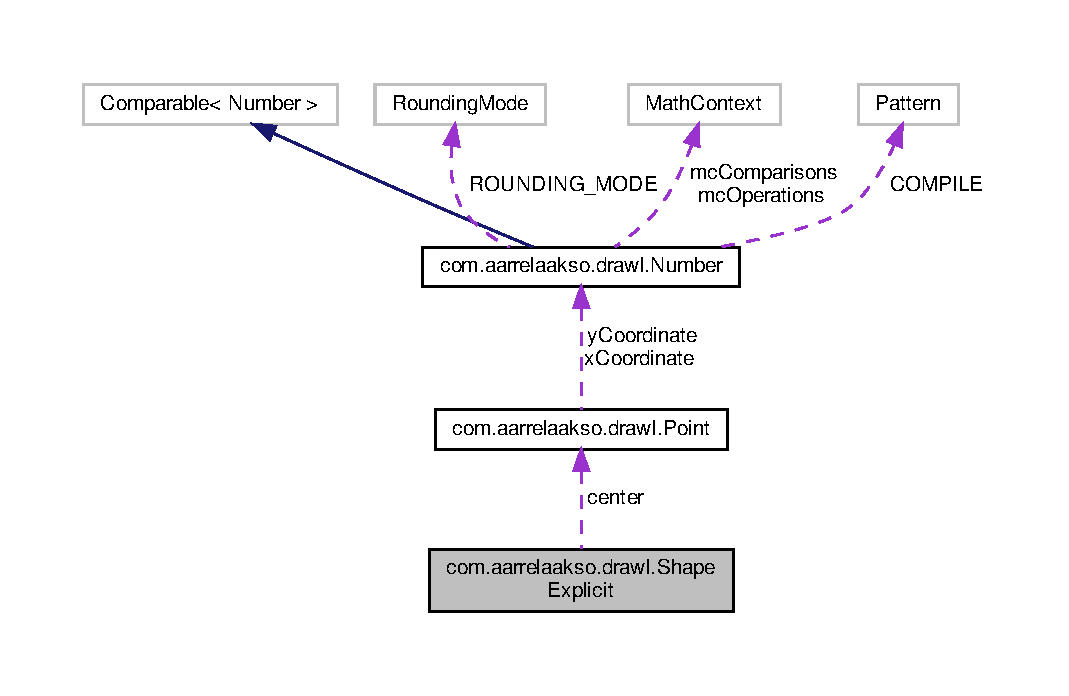
\includegraphics[width=350pt]{de/d31/classcom_1_1aarrelaakso_1_1drawl_1_1_shape_explicit__coll__graph}
\end{center}
\end{figure}
\subsection*{Private Attributes}
\begin{DoxyCompactItemize}
\item 
\hyperlink{classcom_1_1aarrelaakso_1_1drawl_1_1_point}{Point} \hyperlink{classcom_1_1aarrelaakso_1_1drawl_1_1_shape_explicit_aecea9209d9d5d5803acd7ff7b8ec9642}{center}
\end{DoxyCompactItemize}


\subsection{Member Data Documentation}
\mbox{\Hypertarget{classcom_1_1aarrelaakso_1_1drawl_1_1_shape_explicit_aecea9209d9d5d5803acd7ff7b8ec9642}\label{classcom_1_1aarrelaakso_1_1drawl_1_1_shape_explicit_aecea9209d9d5d5803acd7ff7b8ec9642}} 
\index{com\+::aarrelaakso\+::drawl\+::\+Shape\+Explicit@{com\+::aarrelaakso\+::drawl\+::\+Shape\+Explicit}!center@{center}}
\index{center@{center}!com\+::aarrelaakso\+::drawl\+::\+Shape\+Explicit@{com\+::aarrelaakso\+::drawl\+::\+Shape\+Explicit}}
\subsubsection{\texorpdfstring{center}{center}}
{\footnotesize\ttfamily \hyperlink{classcom_1_1aarrelaakso_1_1drawl_1_1_point}{Point} com.\+aarrelaakso.\+drawl.\+Shape\+Explicit.\+center\hspace{0.3cm}{\ttfamily [private]}}



The documentation for this class was generated from the following file\+:\begin{DoxyCompactItemize}
\item 
/mnt/d/\+One\+Drive/\+Documents/src/drawl/src/main/java/com/aarrelaakso/drawl/\hyperlink{_shape_explicit_8java}{Shape\+Explicit.\+java}\end{DoxyCompactItemize}

\hypertarget{classcom_1_1aarrelaakso_1_1drawl_1_1_sisu_number}{}\section{com.\+aarrelaakso.\+drawl.\+Sisu\+Number Class Reference}
\label{classcom_1_1aarrelaakso_1_1drawl_1_1_sisu_number}\index{com.\+aarrelaakso.\+drawl.\+Sisu\+Number@{com.\+aarrelaakso.\+drawl.\+Sisu\+Number}}


Class for mathematical operations with Big\+Decimal values that are not provided by the Big\+Decimal class itself.  




Inheritance diagram for com.\+aarrelaakso.\+drawl.\+Sisu\+Number\+:\nopagebreak
\begin{figure}[H]
\begin{center}
\leavevmode
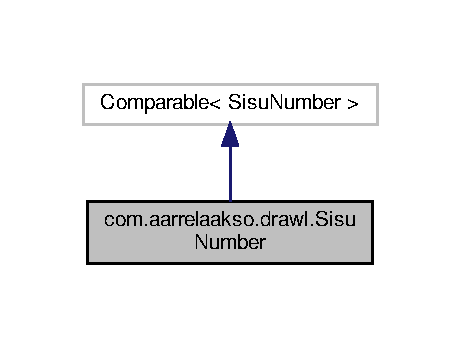
\includegraphics[width=221pt]{df/d65/classcom_1_1aarrelaakso_1_1drawl_1_1_sisu_number__inherit__graph}
\end{center}
\end{figure}


Collaboration diagram for com.\+aarrelaakso.\+drawl.\+Sisu\+Number\+:\nopagebreak
\begin{figure}[H]
\begin{center}
\leavevmode
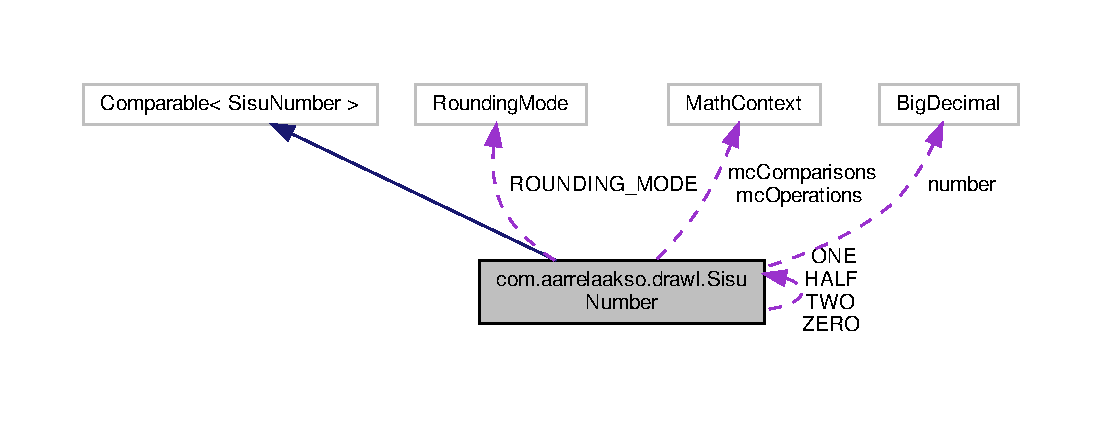
\includegraphics[width=350pt]{df/d10/classcom_1_1aarrelaakso_1_1drawl_1_1_sisu_number__coll__graph}
\end{center}
\end{figure}
\subsection*{Public Member Functions}
\begin{DoxyCompactItemize}
\item 
int \hyperlink{classcom_1_1aarrelaakso_1_1drawl_1_1_sisu_number_a554f83d5273ba11b53e1c82743a7ece0}{compare\+To} (@Not\+Null final \hyperlink{classcom_1_1aarrelaakso_1_1drawl_1_1_sisu_number}{Sisu\+Number} val)
\begin{DoxyCompactList}\small\item\em Compares this Big\+Decimal with the specified Big\+Decimal. \end{DoxyCompactList}\item 
boolean \hyperlink{classcom_1_1aarrelaakso_1_1drawl_1_1_sisu_number_afb509c2c09d10318b136e4defbedd47e}{equals} (final Object obj)
\begin{DoxyCompactList}\small\item\em Compares this \hyperlink{classcom_1_1aarrelaakso_1_1drawl_1_1_sisu_number}{Sisu\+Number} with the specified Object for equality. \end{DoxyCompactList}\item 
int \hyperlink{classcom_1_1aarrelaakso_1_1drawl_1_1_sisu_number_a84f5852d7f79f865cc51d710d09b7032}{hash\+Code} ()
\begin{DoxyCompactList}\small\item\em Returns the hash code for this \hyperlink{classcom_1_1aarrelaakso_1_1drawl_1_1_sisu_number}{Sisu\+Number}. \end{DoxyCompactList}\item 
String \hyperlink{classcom_1_1aarrelaakso_1_1drawl_1_1_sisu_number_a0ed133b435cf93b55afbecb6d28e6cd6}{to\+String} ()
\end{DoxyCompactItemize}
\subsection*{Protected Member Functions}
\begin{DoxyCompactItemize}
\item 
\hyperlink{classcom_1_1aarrelaakso_1_1drawl_1_1_sisu_number_a65081a1817d003c1f9b9dfa8d96af2f1}{Sisu\+Number} (@Not\+Null final Big\+Decimal \hyperlink{classcom_1_1aarrelaakso_1_1drawl_1_1_sisu_number_a5741c4131458787e3adb0bfe649d7758}{number})
\begin{DoxyCompactList}\small\item\em Creates new instance. \end{DoxyCompactList}\item 
\hyperlink{classcom_1_1aarrelaakso_1_1drawl_1_1_sisu_number}{Sisu\+Number} \hyperlink{classcom_1_1aarrelaakso_1_1drawl_1_1_sisu_number_ab0fbcc012471bbf5dc73166c9e27c66c}{abs} ()
\begin{DoxyCompactList}\small\item\em Returns absolute value of this number. \end{DoxyCompactList}\item 
\hyperlink{classcom_1_1aarrelaakso_1_1drawl_1_1_sisu_number}{Sisu\+Number} \hyperlink{classcom_1_1aarrelaakso_1_1drawl_1_1_sisu_number_aae549e52d35575127f6bd52a31d2b2a1}{add} (@Not\+Null final \hyperlink{classcom_1_1aarrelaakso_1_1drawl_1_1_sisu_number}{Sisu\+Number} x)
\begin{DoxyCompactList}\small\item\em Performs addition operation. \end{DoxyCompactList}\item 
\hyperlink{classcom_1_1aarrelaakso_1_1drawl_1_1_sisu_number}{Sisu\+Number} \hyperlink{classcom_1_1aarrelaakso_1_1drawl_1_1_sisu_number_ab3743d41ecc3be5c0e8ca01f958fd166}{add} (final double x)
\begin{DoxyCompactList}\small\item\em Performs addition operation. \end{DoxyCompactList}\item 
\hyperlink{classcom_1_1aarrelaakso_1_1drawl_1_1_sisu_number}{Sisu\+Number} \hyperlink{classcom_1_1aarrelaakso_1_1drawl_1_1_sisu_number_abb2250aca90eb9a85d81c8d83c811a54}{add} (@Not\+Null final \hyperlink{classcom_1_1aarrelaakso_1_1drawl_1_1_sisu_number}{Sisu\+Number} augend, final Math\+Context mc)
\begin{DoxyCompactList}\small\item\em Returns a \hyperlink{classcom_1_1aarrelaakso_1_1drawl_1_1_sisu_number}{Sisu\+Number} whose value is (this + augend), with rounding according to the context settings. \end{DoxyCompactList}\item 
Big\+Decimal \hyperlink{classcom_1_1aarrelaakso_1_1drawl_1_1_sisu_number_a75650999d142612f813ee7ba74ca1318}{big\+Decimal\+Value} ()
\begin{DoxyCompactList}\small\item\em Converts this \hyperlink{classcom_1_1aarrelaakso_1_1drawl_1_1_sisu_number}{Sisu\+Number} to a Big\+Decimal. \end{DoxyCompactList}\item 
int \hyperlink{classcom_1_1aarrelaakso_1_1drawl_1_1_sisu_number_ab061427f9847de3dfd0cb241abd3cd33}{compare\+To\+Fuzzy} (@Not\+Null final \hyperlink{classcom_1_1aarrelaakso_1_1drawl_1_1_sisu_number}{Sisu\+Number} val)
\begin{DoxyCompactList}\small\item\em Compare this Sisus\+Big\+Int to another using the default Math\+Context. \end{DoxyCompactList}\item 
int \hyperlink{classcom_1_1aarrelaakso_1_1drawl_1_1_sisu_number_a0835c9bb9e1bba532983d61844b37109}{compare\+To\+Fuzzy} (@Not\+Null final \hyperlink{classcom_1_1aarrelaakso_1_1drawl_1_1_sisu_number}{Sisu\+Number} val, final Math\+Context mc)
\begin{DoxyCompactList}\small\item\em Compare this \hyperlink{classcom_1_1aarrelaakso_1_1drawl_1_1_sisu_number}{Sisu\+Number} to another fuzzily. \end{DoxyCompactList}\item 
\hyperlink{classcom_1_1aarrelaakso_1_1drawl_1_1_sisu_number}{Sisu\+Number} \hyperlink{classcom_1_1aarrelaakso_1_1drawl_1_1_sisu_number_a79b82b6be0a884a272b80d3462fb0c17}{divide} (@Not\+Null final \hyperlink{classcom_1_1aarrelaakso_1_1drawl_1_1_sisu_number}{Sisu\+Number} val, final Math\+Context math\+Context)
\item 
\hyperlink{classcom_1_1aarrelaakso_1_1drawl_1_1_sisu_number}{Sisu\+Number} \hyperlink{classcom_1_1aarrelaakso_1_1drawl_1_1_sisu_number_ab081d05ed15ab685b2dca36a987d5f63}{divide} (@Not\+Null final \hyperlink{classcom_1_1aarrelaakso_1_1drawl_1_1_sisu_number}{Sisu\+Number} x, final int precision)
\begin{DoxyCompactList}\small\item\em Performs division operation. \end{DoxyCompactList}\item 
\hyperlink{classcom_1_1aarrelaakso_1_1drawl_1_1_sisu_number}{Sisu\+Number} \hyperlink{classcom_1_1aarrelaakso_1_1drawl_1_1_sisu_number_a1d3eea8f14d4700647f1c21cfe366593}{divide} (final double x, final int precision)
\begin{DoxyCompactList}\small\item\em Performs division operation. \end{DoxyCompactList}\item 
double \hyperlink{classcom_1_1aarrelaakso_1_1drawl_1_1_sisu_number_a2ec0d89a34f60f2283ea189a1ae951c1}{double\+Value} ()
\begin{DoxyCompactList}\small\item\em Returns double representation of this number. \end{DoxyCompactList}\item 
boolean \hyperlink{classcom_1_1aarrelaakso_1_1drawl_1_1_sisu_number_a9e6fe0faefc1721b27b4c53f5d8d93ea}{equals} (@Not\+Null final \hyperlink{classcom_1_1aarrelaakso_1_1drawl_1_1_sisu_number}{Sisu\+Number} x)
\begin{DoxyCompactList}\small\item\em Returns whether this number is equal with the other number. \end{DoxyCompactList}\item 
boolean \hyperlink{classcom_1_1aarrelaakso_1_1drawl_1_1_sisu_number_afb83c3ee221f4b839bae842d39ae9067}{equals} (final double x)
\begin{DoxyCompactList}\small\item\em Returns whether this number is equal with the other number. \end{DoxyCompactList}\item 
Float \hyperlink{classcom_1_1aarrelaakso_1_1drawl_1_1_sisu_number_a4c7db66d6d3016a3d10a1664b43117b9}{float\+Value} ()
\begin{DoxyCompactList}\small\item\em Converts this Big\+Decimal to a Float. \end{DoxyCompactList}\item 
boolean \hyperlink{classcom_1_1aarrelaakso_1_1drawl_1_1_sisu_number_a453cb4d7609c2ea7aa0360477e88b6c4}{is\+Greater\+Than} (@Not\+Null final \hyperlink{classcom_1_1aarrelaakso_1_1drawl_1_1_sisu_number}{Sisu\+Number} x)
\begin{DoxyCompactList}\small\item\em Returns whether this number is greater than the other number. \end{DoxyCompactList}\item 
boolean \hyperlink{classcom_1_1aarrelaakso_1_1drawl_1_1_sisu_number_a3910d3f0a3a3de0eea7261eed941742b}{is\+Greater\+Than} (final double x)
\begin{DoxyCompactList}\small\item\em Returns whether this number is greater than the other number. \end{DoxyCompactList}\item 
Integer \hyperlink{classcom_1_1aarrelaakso_1_1drawl_1_1_sisu_number_aa47667c48867cb223722df6facb0da42}{int\+Value} ()
\begin{DoxyCompactList}\small\item\em Converts this Big\+Decimal to an int. \end{DoxyCompactList}\item 
boolean \hyperlink{classcom_1_1aarrelaakso_1_1drawl_1_1_sisu_number_a155f10efc361b9c5b3baf64604aba9f0}{is\+Equal\+To} (@Not\+Null final \hyperlink{classcom_1_1aarrelaakso_1_1drawl_1_1_sisu_number}{Sisu\+Number} x)
\begin{DoxyCompactList}\small\item\em Returns whether this number is equal with another number. \end{DoxyCompactList}\item 
boolean \hyperlink{classcom_1_1aarrelaakso_1_1drawl_1_1_sisu_number_ac64e4cbed7b630a61fa7707a4dbcbd68}{is\+Greater\+Than\+Or\+Equal\+To} (@Not\+Null final \hyperlink{classcom_1_1aarrelaakso_1_1drawl_1_1_sisu_number}{Sisu\+Number} x)
\begin{DoxyCompactList}\small\item\em Returns whether this number is greater or equal to the other number. \end{DoxyCompactList}\item 
boolean \hyperlink{classcom_1_1aarrelaakso_1_1drawl_1_1_sisu_number_a62cf6cef49aa597e48a87ecd9b37650e}{is\+Greater\+Than\+Or\+Equal\+To} (final double x)
\begin{DoxyCompactList}\small\item\em Returns whether this number is greater or equal to the other number. \end{DoxyCompactList}\item 
boolean \hyperlink{classcom_1_1aarrelaakso_1_1drawl_1_1_sisu_number_a58e0ccfb02e7bf83e7c2773e5dc94797}{is\+Less\+Than\+Or\+Equal\+To} (@Not\+Null final \hyperlink{classcom_1_1aarrelaakso_1_1drawl_1_1_sisu_number}{Sisu\+Number} x)
\begin{DoxyCompactList}\small\item\em Returns whether this number is less or equal to the other number. \end{DoxyCompactList}\item 
boolean \hyperlink{classcom_1_1aarrelaakso_1_1drawl_1_1_sisu_number_a540f0064d0baf65b1f783758bb2b5e2c}{is\+Less\+Than\+Or\+Equal\+To} (final double x)
\begin{DoxyCompactList}\small\item\em Returns whether this number is less or equal to the other number. \end{DoxyCompactList}\item 
Boolean \hyperlink{classcom_1_1aarrelaakso_1_1drawl_1_1_sisu_number_a883076b9744036998096851169a09ff4}{is\+Not\+Equal\+To} (@Not\+Null final \hyperlink{classcom_1_1aarrelaakso_1_1drawl_1_1_sisu_number}{Sisu\+Number} val)
\begin{DoxyCompactList}\small\item\em Indicates whether another value is not equal to this \hyperlink{classcom_1_1aarrelaakso_1_1drawl_1_1_sisu_number}{Sisu\+Number}. \end{DoxyCompactList}\item 
boolean \hyperlink{classcom_1_1aarrelaakso_1_1drawl_1_1_sisu_number_ada4f742aeff0f73e1257a8f7254714c9}{is\+Less\+Than} (@Not\+Null final \hyperlink{classcom_1_1aarrelaakso_1_1drawl_1_1_sisu_number}{Sisu\+Number} x)
\begin{DoxyCompactList}\small\item\em Returns whether this number is less than the other number. \end{DoxyCompactList}\item 
boolean \hyperlink{classcom_1_1aarrelaakso_1_1drawl_1_1_sisu_number_aa636492e0db290bbf9a0e58562346f2a}{is\+Less\+Than} (final double x)
\begin{DoxyCompactList}\small\item\em Returns whether this number is less than the other number. \end{DoxyCompactList}\item 
\hyperlink{classcom_1_1aarrelaakso_1_1drawl_1_1_sisu_number}{Sisu\+Number} \hyperlink{classcom_1_1aarrelaakso_1_1drawl_1_1_sisu_number_a0afac67b8a6e28baa04f762c1fd64e64}{multiply} (@Not\+Null final \hyperlink{classcom_1_1aarrelaakso_1_1drawl_1_1_sisu_number}{Sisu\+Number} x)
\begin{DoxyCompactList}\small\item\em Performs multiplication operation. \end{DoxyCompactList}\item 
\hyperlink{classcom_1_1aarrelaakso_1_1drawl_1_1_sisu_number}{Sisu\+Number} \hyperlink{classcom_1_1aarrelaakso_1_1drawl_1_1_sisu_number_ab6665d252e9ea749316cb123846ea476}{multiply} (@Not\+Null final \hyperlink{classcom_1_1aarrelaakso_1_1drawl_1_1_sisu_number}{Sisu\+Number} multiplicand, final Math\+Context mc)
\begin{DoxyCompactList}\small\item\em Returns a Big\+Decimal whose value is (this × multiplicand), with rounding according to the context settings. \end{DoxyCompactList}\item 
\hyperlink{classcom_1_1aarrelaakso_1_1drawl_1_1_sisu_number}{Sisu\+Number} \hyperlink{classcom_1_1aarrelaakso_1_1drawl_1_1_sisu_number_ac95dad537574d5b991f658181e27a0e3}{multiply} (final double x)
\begin{DoxyCompactList}\small\item\em Performs multiplication operation. \end{DoxyCompactList}\item 
\hyperlink{classcom_1_1aarrelaakso_1_1drawl_1_1_sisu_number}{Sisu\+Number} \hyperlink{classcom_1_1aarrelaakso_1_1drawl_1_1_sisu_number_a2386c00d733c84ee7c97ae11d7d05ea8}{negate} ()
\begin{DoxyCompactList}\small\item\em Negates this number. \end{DoxyCompactList}\item 
\hyperlink{classcom_1_1aarrelaakso_1_1drawl_1_1_sisu_number}{Sisu\+Number} \hyperlink{classcom_1_1aarrelaakso_1_1drawl_1_1_sisu_number_a72dee08eae0e9522da081b0c67481b44}{pow} (final int n, final int precision)
\begin{DoxyCompactList}\small\item\em Returns this number powered by n. \end{DoxyCompactList}\item 
\hyperlink{classcom_1_1aarrelaakso_1_1drawl_1_1_sisu_number}{Sisu\+Number} \hyperlink{classcom_1_1aarrelaakso_1_1drawl_1_1_sisu_number_ad3965ead995f42b7f2c52421f69bba7e}{round} (final Math\+Context mc)
\begin{DoxyCompactList}\small\item\em Create a new instance that has same value as this one rounded. \end{DoxyCompactList}\item 
\hyperlink{classcom_1_1aarrelaakso_1_1drawl_1_1_sisu_number}{Sisu\+Number} \hyperlink{classcom_1_1aarrelaakso_1_1drawl_1_1_sisu_number_a3c4d186b36b3eb9efac741e435f94024}{set\+Scale} (final Integer scale)
\begin{DoxyCompactList}\small\item\em Create a new instance with a set scale. \end{DoxyCompactList}\item 
\hyperlink{classcom_1_1aarrelaakso_1_1drawl_1_1_sisu_number}{Sisu\+Number} \hyperlink{classcom_1_1aarrelaakso_1_1drawl_1_1_sisu_number_a09a313ba215327b1e59528090e2632a1}{subtract} (@Not\+Null final \hyperlink{classcom_1_1aarrelaakso_1_1drawl_1_1_sisu_number}{Sisu\+Number} x)
\begin{DoxyCompactList}\small\item\em Performs subtraction operation. \end{DoxyCompactList}\item 
\hyperlink{classcom_1_1aarrelaakso_1_1drawl_1_1_sisu_number}{Sisu\+Number} \hyperlink{classcom_1_1aarrelaakso_1_1drawl_1_1_sisu_number_aec3ddec2b485920d5fe75707f40793e8}{subtract} (@Not\+Null final \hyperlink{classcom_1_1aarrelaakso_1_1drawl_1_1_sisu_number}{Sisu\+Number} subtrahend, final Math\+Context mc)
\begin{DoxyCompactList}\small\item\em Returns a Big\+Decimal whose value is (this -\/ subtrahend), with rounding according to the context settings. \end{DoxyCompactList}\item 
\hyperlink{classcom_1_1aarrelaakso_1_1drawl_1_1_sisu_number}{Sisu\+Number} \hyperlink{classcom_1_1aarrelaakso_1_1drawl_1_1_sisu_number_ab152fb0010ff0cee6a4f94a157c58a02}{subtract} (final double x)
\begin{DoxyCompactList}\small\item\em Performs subtraction operation. \end{DoxyCompactList}\item 
String \hyperlink{classcom_1_1aarrelaakso_1_1drawl_1_1_sisu_number_a487c37a577a8b4a52e86832a32bc303d}{to\+Fixed\+Decimal\+String} (final int num\+Decimals)
\begin{DoxyCompactList}\small\item\em Converts number to the string with fixed decimal digits. \end{DoxyCompactList}\item 
String \hyperlink{classcom_1_1aarrelaakso_1_1drawl_1_1_sisu_number_af92a070f5f79dbd684b2c1b8cf423c6f}{to\+Full\+String} ()
\item 
String \hyperlink{classcom_1_1aarrelaakso_1_1drawl_1_1_sisu_number_af5251e6a7d1f5ed6762394384f2ec604}{to\+Plain\+String} ()
\item 
\hyperlink{classcom_1_1aarrelaakso_1_1drawl_1_1_sisu_number}{Sisu\+Number} \hyperlink{classcom_1_1aarrelaakso_1_1drawl_1_1_sisu_number_ad237bd3a51bc78b3e8cf78d53c1d09c9}{trunc\+Decimals} ()
\begin{DoxyCompactList}\small\item\em Truncates all the fractional part of this number. \end{DoxyCompactList}\end{DoxyCompactItemize}
\subsection*{Static Protected Member Functions}
\begin{DoxyCompactItemize}
\item 
static \hyperlink{classcom_1_1aarrelaakso_1_1drawl_1_1_sisu_number}{Sisu\+Number} \hyperlink{classcom_1_1aarrelaakso_1_1drawl_1_1_sisu_number_abf3f63611bbeb0505b3d6217ba140f9b}{value\+Of} (@Not\+Null final String s)
\begin{DoxyCompactList}\small\item\em Creates new instance. \end{DoxyCompactList}\item 
static \hyperlink{classcom_1_1aarrelaakso_1_1drawl_1_1_sisu_number}{Sisu\+Number} \hyperlink{classcom_1_1aarrelaakso_1_1drawl_1_1_sisu_number_ad51fc8c36a8e9d3dcca80dd633631904}{value\+Of} (final double \hyperlink{classcom_1_1aarrelaakso_1_1drawl_1_1_sisu_number_a5741c4131458787e3adb0bfe649d7758}{number})
\begin{DoxyCompactList}\small\item\em Creates new instance. \end{DoxyCompactList}\item 
static \hyperlink{classcom_1_1aarrelaakso_1_1drawl_1_1_sisu_number}{Sisu\+Number} \hyperlink{classcom_1_1aarrelaakso_1_1drawl_1_1_sisu_number_ad12beb94319a712de494e2710620031f}{value\+Of} (@Not\+Null final Big\+Decimal \hyperlink{classcom_1_1aarrelaakso_1_1drawl_1_1_sisu_number_a5741c4131458787e3adb0bfe649d7758}{number})
\begin{DoxyCompactList}\small\item\em Creates new instance. \end{DoxyCompactList}\item 
static \hyperlink{classcom_1_1aarrelaakso_1_1drawl_1_1_sisu_number}{Sisu\+Number} \hyperlink{classcom_1_1aarrelaakso_1_1drawl_1_1_sisu_number_aff49a9d0e8fa7aa03b45a15ee2365bb6}{value\+Of} (final Integer \hyperlink{classcom_1_1aarrelaakso_1_1drawl_1_1_sisu_number_a5741c4131458787e3adb0bfe649d7758}{number})
\item 
static boolean \hyperlink{classcom_1_1aarrelaakso_1_1drawl_1_1_sisu_number_a6fd0fcaee1f9723b48fbea1200f96414}{is\+Integer\+Value} (@Not\+Null final Big\+Decimal bd)
\begin{DoxyCompactList}\small\item\em Test whether a Big\+Decimal is a mathematical integer. \end{DoxyCompactList}\item 
static boolean \hyperlink{classcom_1_1aarrelaakso_1_1drawl_1_1_sisu_number_ab2ea066abe7a6f8f565ebfc7ac382b28}{is\+Integer\+Value} (final float val)
\begin{DoxyCompactList}\small\item\em Test whether a float is a mathematical integer. \end{DoxyCompactList}\end{DoxyCompactItemize}
\subsection*{Static Protected Attributes}
\begin{DoxyCompactItemize}
\item 
static final \hyperlink{classcom_1_1aarrelaakso_1_1drawl_1_1_sisu_number}{Sisu\+Number} \hyperlink{classcom_1_1aarrelaakso_1_1drawl_1_1_sisu_number_afae3e6d652b8c125dccab3e110d038b0}{H\+A\+LF} = \hyperlink{classcom_1_1aarrelaakso_1_1drawl_1_1_sisu_number_abf3f63611bbeb0505b3d6217ba140f9b}{value\+Of}(0.\+5)
\item 
static final \hyperlink{classcom_1_1aarrelaakso_1_1drawl_1_1_sisu_number}{Sisu\+Number} \hyperlink{classcom_1_1aarrelaakso_1_1drawl_1_1_sisu_number_ad74e537df980406b3282861605df259c}{O\+NE} = \hyperlink{classcom_1_1aarrelaakso_1_1drawl_1_1_sisu_number_abf3f63611bbeb0505b3d6217ba140f9b}{value\+Of}(Big\+Decimal.\+O\+NE)
\item 
static final \hyperlink{classcom_1_1aarrelaakso_1_1drawl_1_1_sisu_number}{Sisu\+Number} \hyperlink{classcom_1_1aarrelaakso_1_1drawl_1_1_sisu_number_a699eb6b7e4648b4a8d888890b32e26f9}{T\+WO} = \hyperlink{classcom_1_1aarrelaakso_1_1drawl_1_1_sisu_number_abf3f63611bbeb0505b3d6217ba140f9b}{value\+Of}(2)
\item 
static \hyperlink{classcom_1_1aarrelaakso_1_1drawl_1_1_sisu_number}{Sisu\+Number} \hyperlink{classcom_1_1aarrelaakso_1_1drawl_1_1_sisu_number_ae9e547c1510ee19d5cc6401c828f1003}{Z\+E\+RO} = new \hyperlink{classcom_1_1aarrelaakso_1_1drawl_1_1_sisu_number}{Sisu\+Number}(\char`\"{}0\char`\"{})
\begin{DoxyCompactList}\small\item\em Zero. \end{DoxyCompactList}\item 
static Math\+Context \hyperlink{classcom_1_1aarrelaakso_1_1drawl_1_1_sisu_number_a09a6e4440f1be870727ad0bc028fc237}{mc\+Comparisons} = new Math\+Context(\hyperlink{classcom_1_1aarrelaakso_1_1drawl_1_1_sisu_number_a4630f8f5414673cb5021dc7d194dc257}{Sisu\+Number.\+S\+C\+A\+L\+E\+\_\+\+F\+O\+R\+\_\+\+C\+O\+M\+P\+A\+R\+I\+S\+O\+NS}, \hyperlink{classcom_1_1aarrelaakso_1_1drawl_1_1_sisu_number_a98077c422e928740febf571e3f2ec6b5}{Sisu\+Number.\+R\+O\+U\+N\+D\+I\+N\+G\+\_\+\+M\+O\+DE})
\begin{DoxyCompactList}\small\item\em Use this Math\+Context for comparisons. \end{DoxyCompactList}\item 
static Math\+Context \hyperlink{classcom_1_1aarrelaakso_1_1drawl_1_1_sisu_number_a526b69c7921d715b6b49ad98ecf442fc}{mc\+Operations} = new Math\+Context(\hyperlink{classcom_1_1aarrelaakso_1_1drawl_1_1_sisu_number_a0ab71e0c4e4143159d9341c562d131af}{Sisu\+Number.\+S\+C\+A\+L\+E\+\_\+\+F\+O\+R\+\_\+\+O\+P\+E\+R\+A\+T\+I\+O\+NS}, \hyperlink{classcom_1_1aarrelaakso_1_1drawl_1_1_sisu_number_a98077c422e928740febf571e3f2ec6b5}{Sisu\+Number.\+R\+O\+U\+N\+D\+I\+N\+G\+\_\+\+M\+O\+DE})
\begin{DoxyCompactList}\small\item\em Use this Math\+Context for other operations, such as multiplying and dividing. \end{DoxyCompactList}\end{DoxyCompactItemize}
\subsection*{Private Member Functions}
\begin{DoxyCompactItemize}
\item 
\hyperlink{classcom_1_1aarrelaakso_1_1drawl_1_1_sisu_number_a3e7b40170c4ae69461b94208a0f82f5e}{Sisu\+Number} ()
\begin{DoxyCompactList}\small\item\em Prevents construction from outside. \end{DoxyCompactList}\item 
\hyperlink{classcom_1_1aarrelaakso_1_1drawl_1_1_sisu_number_acd07ad566abfb66de69b21bb1b31c189}{Sisu\+Number} (@Not\+Null final String s)
\begin{DoxyCompactList}\small\item\em Creates new instance. \end{DoxyCompactList}\item 
int \hyperlink{classcom_1_1aarrelaakso_1_1drawl_1_1_sisu_number_a846e0834c619e63a8d85579484ab4276}{temp} ()
\begin{DoxyCompactList}\small\item\em Returns the string representation of this \hyperlink{classcom_1_1aarrelaakso_1_1drawl_1_1_sisu_number}{Sisu\+Number}, using scientific notation if an exponent is needed. \end{DoxyCompactList}\end{DoxyCompactItemize}
\subsection*{Private Attributes}
\begin{DoxyCompactItemize}
\item 
Big\+Decimal \hyperlink{classcom_1_1aarrelaakso_1_1drawl_1_1_sisu_number_a5741c4131458787e3adb0bfe649d7758}{number}
\begin{DoxyCompactList}\small\item\em Precise number representation. \end{DoxyCompactList}\end{DoxyCompactItemize}
\subsection*{Static Private Attributes}
\begin{DoxyCompactItemize}
\item 
static Rounding\+Mode \hyperlink{classcom_1_1aarrelaakso_1_1drawl_1_1_sisu_number_a98077c422e928740febf571e3f2ec6b5}{R\+O\+U\+N\+D\+I\+N\+G\+\_\+\+M\+O\+DE} = Rounding\+Mode.\+H\+A\+L\+F\+\_\+\+UP
\item 
static final int \hyperlink{classcom_1_1aarrelaakso_1_1drawl_1_1_sisu_number_a4630f8f5414673cb5021dc7d194dc257}{S\+C\+A\+L\+E\+\_\+\+F\+O\+R\+\_\+\+C\+O\+M\+P\+A\+R\+I\+S\+O\+NS} = 32
\item 
static final int \hyperlink{classcom_1_1aarrelaakso_1_1drawl_1_1_sisu_number_a0ab71e0c4e4143159d9341c562d131af}{S\+C\+A\+L\+E\+\_\+\+F\+O\+R\+\_\+\+O\+P\+E\+R\+A\+T\+I\+O\+NS} = 64
\end{DoxyCompactItemize}


\subsection{Detailed Description}
Class for mathematical operations with Big\+Decimal values that are not provided by the Big\+Decimal class itself. 

Like a Big\+Decimal, a \hyperlink{classcom_1_1aarrelaakso_1_1drawl_1_1_sisu_number}{Sisu\+Number} consists of an arbitrary precision integer unscaled value and a 32-\/bit integer scale. If zero or positive, the scale is the number of digits to the right of the decimal point. If negative, the unscaled value of the number is multiplied by ten to the power of the negation of the scale. The value of the number represented by the Big\+Decimal is therefore (unscaled\+Value × 10$^\wedge$scale). 

In this class precision has same meaning as in the standard java Big\+Decimal class. That means number of digits representing the number counted from to most left non zero one.

\begin{DoxyAuthor}{Author}
radek.\+hecl  \href{https://dzone.com/articles/arbitrary-precision-numbers}{\tt https\+://dzone.\+com/articles/arbitrary-\/precision-\/numbers} 
\end{DoxyAuthor}


\subsection{Constructor \& Destructor Documentation}
\mbox{\Hypertarget{classcom_1_1aarrelaakso_1_1drawl_1_1_sisu_number_a3e7b40170c4ae69461b94208a0f82f5e}\label{classcom_1_1aarrelaakso_1_1drawl_1_1_sisu_number_a3e7b40170c4ae69461b94208a0f82f5e}} 
\index{com\+::aarrelaakso\+::drawl\+::\+Sisu\+Number@{com\+::aarrelaakso\+::drawl\+::\+Sisu\+Number}!Sisu\+Number@{Sisu\+Number}}
\index{Sisu\+Number@{Sisu\+Number}!com\+::aarrelaakso\+::drawl\+::\+Sisu\+Number@{com\+::aarrelaakso\+::drawl\+::\+Sisu\+Number}}
\subsubsection{\texorpdfstring{Sisu\+Number()}{SisuNumber()}\hspace{0.1cm}{\footnotesize\ttfamily [1/3]}}
{\footnotesize\ttfamily com.\+aarrelaakso.\+drawl.\+Sisu\+Number.\+Sisu\+Number (\begin{DoxyParamCaption}{ }\end{DoxyParamCaption})\hspace{0.3cm}{\ttfamily [private]}}



Prevents construction from outside. 

\mbox{\Hypertarget{classcom_1_1aarrelaakso_1_1drawl_1_1_sisu_number_a65081a1817d003c1f9b9dfa8d96af2f1}\label{classcom_1_1aarrelaakso_1_1drawl_1_1_sisu_number_a65081a1817d003c1f9b9dfa8d96af2f1}} 
\index{com\+::aarrelaakso\+::drawl\+::\+Sisu\+Number@{com\+::aarrelaakso\+::drawl\+::\+Sisu\+Number}!Sisu\+Number@{Sisu\+Number}}
\index{Sisu\+Number@{Sisu\+Number}!com\+::aarrelaakso\+::drawl\+::\+Sisu\+Number@{com\+::aarrelaakso\+::drawl\+::\+Sisu\+Number}}
\subsubsection{\texorpdfstring{Sisu\+Number()}{SisuNumber()}\hspace{0.1cm}{\footnotesize\ttfamily [2/3]}}
{\footnotesize\ttfamily com.\+aarrelaakso.\+drawl.\+Sisu\+Number.\+Sisu\+Number (\begin{DoxyParamCaption}\item[{@Not\+Null final Big\+Decimal}]{number }\end{DoxyParamCaption})\hspace{0.3cm}{\ttfamily [protected]}}



Creates new instance. 


\begin{DoxyParams}{Parameters}
{\em number} & number \\
\hline
\end{DoxyParams}
\mbox{\Hypertarget{classcom_1_1aarrelaakso_1_1drawl_1_1_sisu_number_acd07ad566abfb66de69b21bb1b31c189}\label{classcom_1_1aarrelaakso_1_1drawl_1_1_sisu_number_acd07ad566abfb66de69b21bb1b31c189}} 
\index{com\+::aarrelaakso\+::drawl\+::\+Sisu\+Number@{com\+::aarrelaakso\+::drawl\+::\+Sisu\+Number}!Sisu\+Number@{Sisu\+Number}}
\index{Sisu\+Number@{Sisu\+Number}!com\+::aarrelaakso\+::drawl\+::\+Sisu\+Number@{com\+::aarrelaakso\+::drawl\+::\+Sisu\+Number}}
\subsubsection{\texorpdfstring{Sisu\+Number()}{SisuNumber()}\hspace{0.1cm}{\footnotesize\ttfamily [3/3]}}
{\footnotesize\ttfamily com.\+aarrelaakso.\+drawl.\+Sisu\+Number.\+Sisu\+Number (\begin{DoxyParamCaption}\item[{@Not\+Null final String}]{s }\end{DoxyParamCaption})\hspace{0.3cm}{\ttfamily [private]}}



Creates new instance. 


\begin{DoxyParams}{Parameters}
{\em s} & string representation \\
\hline
\end{DoxyParams}


\subsection{Member Function Documentation}
\mbox{\Hypertarget{classcom_1_1aarrelaakso_1_1drawl_1_1_sisu_number_ab0fbcc012471bbf5dc73166c9e27c66c}\label{classcom_1_1aarrelaakso_1_1drawl_1_1_sisu_number_ab0fbcc012471bbf5dc73166c9e27c66c}} 
\index{com\+::aarrelaakso\+::drawl\+::\+Sisu\+Number@{com\+::aarrelaakso\+::drawl\+::\+Sisu\+Number}!abs@{abs}}
\index{abs@{abs}!com\+::aarrelaakso\+::drawl\+::\+Sisu\+Number@{com\+::aarrelaakso\+::drawl\+::\+Sisu\+Number}}
\subsubsection{\texorpdfstring{abs()}{abs()}}
{\footnotesize\ttfamily \hyperlink{classcom_1_1aarrelaakso_1_1drawl_1_1_sisu_number}{Sisu\+Number} com.\+aarrelaakso.\+drawl.\+Sisu\+Number.\+abs (\begin{DoxyParamCaption}{ }\end{DoxyParamCaption})\hspace{0.3cm}{\ttfamily [protected]}}



Returns absolute value of this number. 

\begin{DoxyReturn}{Returns}
absolute value of this number 
\end{DoxyReturn}
\mbox{\Hypertarget{classcom_1_1aarrelaakso_1_1drawl_1_1_sisu_number_aae549e52d35575127f6bd52a31d2b2a1}\label{classcom_1_1aarrelaakso_1_1drawl_1_1_sisu_number_aae549e52d35575127f6bd52a31d2b2a1}} 
\index{com\+::aarrelaakso\+::drawl\+::\+Sisu\+Number@{com\+::aarrelaakso\+::drawl\+::\+Sisu\+Number}!add@{add}}
\index{add@{add}!com\+::aarrelaakso\+::drawl\+::\+Sisu\+Number@{com\+::aarrelaakso\+::drawl\+::\+Sisu\+Number}}
\subsubsection{\texorpdfstring{add()}{add()}\hspace{0.1cm}{\footnotesize\ttfamily [1/3]}}
{\footnotesize\ttfamily \hyperlink{classcom_1_1aarrelaakso_1_1drawl_1_1_sisu_number}{Sisu\+Number} com.\+aarrelaakso.\+drawl.\+Sisu\+Number.\+add (\begin{DoxyParamCaption}\item[{@Not\+Null final \hyperlink{classcom_1_1aarrelaakso_1_1drawl_1_1_sisu_number}{Sisu\+Number}}]{x }\end{DoxyParamCaption})\hspace{0.3cm}{\ttfamily [protected]}}



Performs addition operation. 


\begin{DoxyParams}{Parameters}
{\em x} & other number \\
\hline
\end{DoxyParams}
\begin{DoxyReturn}{Returns}
addition operation result 
\end{DoxyReturn}
\mbox{\Hypertarget{classcom_1_1aarrelaakso_1_1drawl_1_1_sisu_number_ab3743d41ecc3be5c0e8ca01f958fd166}\label{classcom_1_1aarrelaakso_1_1drawl_1_1_sisu_number_ab3743d41ecc3be5c0e8ca01f958fd166}} 
\index{com\+::aarrelaakso\+::drawl\+::\+Sisu\+Number@{com\+::aarrelaakso\+::drawl\+::\+Sisu\+Number}!add@{add}}
\index{add@{add}!com\+::aarrelaakso\+::drawl\+::\+Sisu\+Number@{com\+::aarrelaakso\+::drawl\+::\+Sisu\+Number}}
\subsubsection{\texorpdfstring{add()}{add()}\hspace{0.1cm}{\footnotesize\ttfamily [2/3]}}
{\footnotesize\ttfamily \hyperlink{classcom_1_1aarrelaakso_1_1drawl_1_1_sisu_number}{Sisu\+Number} com.\+aarrelaakso.\+drawl.\+Sisu\+Number.\+add (\begin{DoxyParamCaption}\item[{final double}]{x }\end{DoxyParamCaption})\hspace{0.3cm}{\ttfamily [protected]}}



Performs addition operation. 


\begin{DoxyParams}{Parameters}
{\em x} & other number \\
\hline
\end{DoxyParams}
\begin{DoxyReturn}{Returns}
addition operation result 
\end{DoxyReturn}
\mbox{\Hypertarget{classcom_1_1aarrelaakso_1_1drawl_1_1_sisu_number_abb2250aca90eb9a85d81c8d83c811a54}\label{classcom_1_1aarrelaakso_1_1drawl_1_1_sisu_number_abb2250aca90eb9a85d81c8d83c811a54}} 
\index{com\+::aarrelaakso\+::drawl\+::\+Sisu\+Number@{com\+::aarrelaakso\+::drawl\+::\+Sisu\+Number}!add@{add}}
\index{add@{add}!com\+::aarrelaakso\+::drawl\+::\+Sisu\+Number@{com\+::aarrelaakso\+::drawl\+::\+Sisu\+Number}}
\subsubsection{\texorpdfstring{add()}{add()}\hspace{0.1cm}{\footnotesize\ttfamily [3/3]}}
{\footnotesize\ttfamily \hyperlink{classcom_1_1aarrelaakso_1_1drawl_1_1_sisu_number}{Sisu\+Number} com.\+aarrelaakso.\+drawl.\+Sisu\+Number.\+add (\begin{DoxyParamCaption}\item[{@Not\+Null final \hyperlink{classcom_1_1aarrelaakso_1_1drawl_1_1_sisu_number}{Sisu\+Number}}]{augend,  }\item[{final Math\+Context}]{mc }\end{DoxyParamCaption})\hspace{0.3cm}{\ttfamily [protected]}}



Returns a \hyperlink{classcom_1_1aarrelaakso_1_1drawl_1_1_sisu_number}{Sisu\+Number} whose value is (this + augend), with rounding according to the context settings. 

If either number is zero and the precision setting is nonzero, then the other number, rounded if necessary, is used as the result.


\begin{DoxyParams}{Parameters}
{\em augend} & value to be added to this \hyperlink{classcom_1_1aarrelaakso_1_1drawl_1_1_sisu_number}{Sisu\+Number}. \\
\hline
{\em mc} & the Math\+Context to use. \\
\hline
\end{DoxyParams}
\begin{DoxyReturn}{Returns}
this + augend, rounded as necessary 
\end{DoxyReturn}

\begin{DoxyExceptions}{Exceptions}
{\em Arithmetic\+Exception} & if the result is inexact but the rounding mode is U\+N\+N\+E\+C\+E\+S\+S\+A\+RY. \\
\hline
\end{DoxyExceptions}
\mbox{\Hypertarget{classcom_1_1aarrelaakso_1_1drawl_1_1_sisu_number_a75650999d142612f813ee7ba74ca1318}\label{classcom_1_1aarrelaakso_1_1drawl_1_1_sisu_number_a75650999d142612f813ee7ba74ca1318}} 
\index{com\+::aarrelaakso\+::drawl\+::\+Sisu\+Number@{com\+::aarrelaakso\+::drawl\+::\+Sisu\+Number}!big\+Decimal\+Value@{big\+Decimal\+Value}}
\index{big\+Decimal\+Value@{big\+Decimal\+Value}!com\+::aarrelaakso\+::drawl\+::\+Sisu\+Number@{com\+::aarrelaakso\+::drawl\+::\+Sisu\+Number}}
\subsubsection{\texorpdfstring{big\+Decimal\+Value()}{bigDecimalValue()}}
{\footnotesize\ttfamily Big\+Decimal com.\+aarrelaakso.\+drawl.\+Sisu\+Number.\+big\+Decimal\+Value (\begin{DoxyParamCaption}{ }\end{DoxyParamCaption})\hspace{0.3cm}{\ttfamily [protected]}}



Converts this \hyperlink{classcom_1_1aarrelaakso_1_1drawl_1_1_sisu_number}{Sisu\+Number} to a Big\+Decimal. 

\begin{DoxyReturn}{Returns}
this \hyperlink{classcom_1_1aarrelaakso_1_1drawl_1_1_sisu_number}{Sisu\+Number} converted to a Big\+Decimal. 
\end{DoxyReturn}
\mbox{\Hypertarget{classcom_1_1aarrelaakso_1_1drawl_1_1_sisu_number_a554f83d5273ba11b53e1c82743a7ece0}\label{classcom_1_1aarrelaakso_1_1drawl_1_1_sisu_number_a554f83d5273ba11b53e1c82743a7ece0}} 
\index{com\+::aarrelaakso\+::drawl\+::\+Sisu\+Number@{com\+::aarrelaakso\+::drawl\+::\+Sisu\+Number}!compare\+To@{compare\+To}}
\index{compare\+To@{compare\+To}!com\+::aarrelaakso\+::drawl\+::\+Sisu\+Number@{com\+::aarrelaakso\+::drawl\+::\+Sisu\+Number}}
\subsubsection{\texorpdfstring{compare\+To()}{compareTo()}}
{\footnotesize\ttfamily int com.\+aarrelaakso.\+drawl.\+Sisu\+Number.\+compare\+To (\begin{DoxyParamCaption}\item[{@Not\+Null final \hyperlink{classcom_1_1aarrelaakso_1_1drawl_1_1_sisu_number}{Sisu\+Number}}]{val }\end{DoxyParamCaption})}



Compares this Big\+Decimal with the specified Big\+Decimal. 

Two Big\+Decimal objects that are equal in value but have a different scale (like 2.\+0 and 2.\+00) are considered equal by this method. 

This method overrides the compare\+To method in the java.\+lang.\+Comparable interface.


\begin{DoxyParams}{Parameters}
{\em val} & Big\+Decimal to which this Big\+Decimal is to be compared. \\
\hline
\end{DoxyParams}
\begin{DoxyReturn}{Returns}
-\/1, 0, or 1 as this Big\+Decimal is numerically less than, equal to, or greater than val. 
\end{DoxyReturn}
\mbox{\Hypertarget{classcom_1_1aarrelaakso_1_1drawl_1_1_sisu_number_ab061427f9847de3dfd0cb241abd3cd33}\label{classcom_1_1aarrelaakso_1_1drawl_1_1_sisu_number_ab061427f9847de3dfd0cb241abd3cd33}} 
\index{com\+::aarrelaakso\+::drawl\+::\+Sisu\+Number@{com\+::aarrelaakso\+::drawl\+::\+Sisu\+Number}!compare\+To\+Fuzzy@{compare\+To\+Fuzzy}}
\index{compare\+To\+Fuzzy@{compare\+To\+Fuzzy}!com\+::aarrelaakso\+::drawl\+::\+Sisu\+Number@{com\+::aarrelaakso\+::drawl\+::\+Sisu\+Number}}
\subsubsection{\texorpdfstring{compare\+To\+Fuzzy()}{compareToFuzzy()}\hspace{0.1cm}{\footnotesize\ttfamily [1/2]}}
{\footnotesize\ttfamily int com.\+aarrelaakso.\+drawl.\+Sisu\+Number.\+compare\+To\+Fuzzy (\begin{DoxyParamCaption}\item[{@Not\+Null final \hyperlink{classcom_1_1aarrelaakso_1_1drawl_1_1_sisu_number}{Sisu\+Number}}]{val }\end{DoxyParamCaption})\hspace{0.3cm}{\ttfamily [protected]}}



Compare this Sisus\+Big\+Int to another using the default Math\+Context. 


\begin{DoxyParams}{Parameters}
{\em val} & The other \hyperlink{classcom_1_1aarrelaakso_1_1drawl_1_1_sisu_number}{Sisu\+Number} to compare to this one. \\
\hline
\end{DoxyParams}
\begin{DoxyReturn}{Returns}
-\/1, 0, or 1 as this Big\+Decimal is numerically less than, equal to, or greater than val. 
\end{DoxyReturn}
\mbox{\Hypertarget{classcom_1_1aarrelaakso_1_1drawl_1_1_sisu_number_a0835c9bb9e1bba532983d61844b37109}\label{classcom_1_1aarrelaakso_1_1drawl_1_1_sisu_number_a0835c9bb9e1bba532983d61844b37109}} 
\index{com\+::aarrelaakso\+::drawl\+::\+Sisu\+Number@{com\+::aarrelaakso\+::drawl\+::\+Sisu\+Number}!compare\+To\+Fuzzy@{compare\+To\+Fuzzy}}
\index{compare\+To\+Fuzzy@{compare\+To\+Fuzzy}!com\+::aarrelaakso\+::drawl\+::\+Sisu\+Number@{com\+::aarrelaakso\+::drawl\+::\+Sisu\+Number}}
\subsubsection{\texorpdfstring{compare\+To\+Fuzzy()}{compareToFuzzy()}\hspace{0.1cm}{\footnotesize\ttfamily [2/2]}}
{\footnotesize\ttfamily int com.\+aarrelaakso.\+drawl.\+Sisu\+Number.\+compare\+To\+Fuzzy (\begin{DoxyParamCaption}\item[{@Not\+Null final \hyperlink{classcom_1_1aarrelaakso_1_1drawl_1_1_sisu_number}{Sisu\+Number}}]{val,  }\item[{final Math\+Context}]{mc }\end{DoxyParamCaption})\hspace{0.3cm}{\ttfamily [protected]}}



Compare this \hyperlink{classcom_1_1aarrelaakso_1_1drawl_1_1_sisu_number}{Sisu\+Number} to another fuzzily. 


\begin{DoxyParams}{Parameters}
{\em val} & The other \hyperlink{classcom_1_1aarrelaakso_1_1drawl_1_1_sisu_number}{Sisu\+Number} to compare to this one. \\
\hline
{\em mc} & The Math\+Context to use for the comparison. \\
\hline
\end{DoxyParams}
\begin{DoxyReturn}{Returns}
-\/1, 0, or 1 as this Big\+Decimal is numerically less than, equal to, or greater than val. 
\end{DoxyReturn}
\mbox{\Hypertarget{classcom_1_1aarrelaakso_1_1drawl_1_1_sisu_number_a79b82b6be0a884a272b80d3462fb0c17}\label{classcom_1_1aarrelaakso_1_1drawl_1_1_sisu_number_a79b82b6be0a884a272b80d3462fb0c17}} 
\index{com\+::aarrelaakso\+::drawl\+::\+Sisu\+Number@{com\+::aarrelaakso\+::drawl\+::\+Sisu\+Number}!divide@{divide}}
\index{divide@{divide}!com\+::aarrelaakso\+::drawl\+::\+Sisu\+Number@{com\+::aarrelaakso\+::drawl\+::\+Sisu\+Number}}
\subsubsection{\texorpdfstring{divide()}{divide()}\hspace{0.1cm}{\footnotesize\ttfamily [1/3]}}
{\footnotesize\ttfamily \hyperlink{classcom_1_1aarrelaakso_1_1drawl_1_1_sisu_number}{Sisu\+Number} com.\+aarrelaakso.\+drawl.\+Sisu\+Number.\+divide (\begin{DoxyParamCaption}\item[{@Not\+Null final \hyperlink{classcom_1_1aarrelaakso_1_1drawl_1_1_sisu_number}{Sisu\+Number}}]{val,  }\item[{final Math\+Context}]{math\+Context }\end{DoxyParamCaption})\hspace{0.3cm}{\ttfamily [protected]}}

\mbox{\Hypertarget{classcom_1_1aarrelaakso_1_1drawl_1_1_sisu_number_ab081d05ed15ab685b2dca36a987d5f63}\label{classcom_1_1aarrelaakso_1_1drawl_1_1_sisu_number_ab081d05ed15ab685b2dca36a987d5f63}} 
\index{com\+::aarrelaakso\+::drawl\+::\+Sisu\+Number@{com\+::aarrelaakso\+::drawl\+::\+Sisu\+Number}!divide@{divide}}
\index{divide@{divide}!com\+::aarrelaakso\+::drawl\+::\+Sisu\+Number@{com\+::aarrelaakso\+::drawl\+::\+Sisu\+Number}}
\subsubsection{\texorpdfstring{divide()}{divide()}\hspace{0.1cm}{\footnotesize\ttfamily [2/3]}}
{\footnotesize\ttfamily \hyperlink{classcom_1_1aarrelaakso_1_1drawl_1_1_sisu_number}{Sisu\+Number} com.\+aarrelaakso.\+drawl.\+Sisu\+Number.\+divide (\begin{DoxyParamCaption}\item[{@Not\+Null final \hyperlink{classcom_1_1aarrelaakso_1_1drawl_1_1_sisu_number}{Sisu\+Number}}]{x,  }\item[{final int}]{precision }\end{DoxyParamCaption})\hspace{0.3cm}{\ttfamily [protected]}}



Performs division operation. 


\begin{DoxyParams}{Parameters}
{\em x} & divisor number \\
\hline
{\em precision} & precision of the result (see the class level comment for details) \\
\hline
\end{DoxyParams}
\begin{DoxyReturn}{Returns}
division operation result 
\end{DoxyReturn}
\mbox{\Hypertarget{classcom_1_1aarrelaakso_1_1drawl_1_1_sisu_number_a1d3eea8f14d4700647f1c21cfe366593}\label{classcom_1_1aarrelaakso_1_1drawl_1_1_sisu_number_a1d3eea8f14d4700647f1c21cfe366593}} 
\index{com\+::aarrelaakso\+::drawl\+::\+Sisu\+Number@{com\+::aarrelaakso\+::drawl\+::\+Sisu\+Number}!divide@{divide}}
\index{divide@{divide}!com\+::aarrelaakso\+::drawl\+::\+Sisu\+Number@{com\+::aarrelaakso\+::drawl\+::\+Sisu\+Number}}
\subsubsection{\texorpdfstring{divide()}{divide()}\hspace{0.1cm}{\footnotesize\ttfamily [3/3]}}
{\footnotesize\ttfamily \hyperlink{classcom_1_1aarrelaakso_1_1drawl_1_1_sisu_number}{Sisu\+Number} com.\+aarrelaakso.\+drawl.\+Sisu\+Number.\+divide (\begin{DoxyParamCaption}\item[{final double}]{x,  }\item[{final int}]{precision }\end{DoxyParamCaption})\hspace{0.3cm}{\ttfamily [protected]}}



Performs division operation. 


\begin{DoxyParams}{Parameters}
{\em x} & divisor number \\
\hline
{\em precision} & precision of the result (see the class level comment for details) \\
\hline
\end{DoxyParams}
\begin{DoxyReturn}{Returns}
division operation result 
\end{DoxyReturn}
\mbox{\Hypertarget{classcom_1_1aarrelaakso_1_1drawl_1_1_sisu_number_a2ec0d89a34f60f2283ea189a1ae951c1}\label{classcom_1_1aarrelaakso_1_1drawl_1_1_sisu_number_a2ec0d89a34f60f2283ea189a1ae951c1}} 
\index{com\+::aarrelaakso\+::drawl\+::\+Sisu\+Number@{com\+::aarrelaakso\+::drawl\+::\+Sisu\+Number}!double\+Value@{double\+Value}}
\index{double\+Value@{double\+Value}!com\+::aarrelaakso\+::drawl\+::\+Sisu\+Number@{com\+::aarrelaakso\+::drawl\+::\+Sisu\+Number}}
\subsubsection{\texorpdfstring{double\+Value()}{doubleValue()}}
{\footnotesize\ttfamily double com.\+aarrelaakso.\+drawl.\+Sisu\+Number.\+double\+Value (\begin{DoxyParamCaption}{ }\end{DoxyParamCaption})\hspace{0.3cm}{\ttfamily [protected]}}



Returns double representation of this number. 

Conversion might ended up by loosing the precision.

\begin{DoxyReturn}{Returns}
double representation of this value 
\end{DoxyReturn}
\mbox{\Hypertarget{classcom_1_1aarrelaakso_1_1drawl_1_1_sisu_number_a9e6fe0faefc1721b27b4c53f5d8d93ea}\label{classcom_1_1aarrelaakso_1_1drawl_1_1_sisu_number_a9e6fe0faefc1721b27b4c53f5d8d93ea}} 
\index{com\+::aarrelaakso\+::drawl\+::\+Sisu\+Number@{com\+::aarrelaakso\+::drawl\+::\+Sisu\+Number}!equals@{equals}}
\index{equals@{equals}!com\+::aarrelaakso\+::drawl\+::\+Sisu\+Number@{com\+::aarrelaakso\+::drawl\+::\+Sisu\+Number}}
\subsubsection{\texorpdfstring{equals()}{equals()}\hspace{0.1cm}{\footnotesize\ttfamily [1/3]}}
{\footnotesize\ttfamily boolean com.\+aarrelaakso.\+drawl.\+Sisu\+Number.\+equals (\begin{DoxyParamCaption}\item[{@Not\+Null final \hyperlink{classcom_1_1aarrelaakso_1_1drawl_1_1_sisu_number}{Sisu\+Number}}]{x }\end{DoxyParamCaption})\hspace{0.3cm}{\ttfamily [protected]}}



Returns whether this number is equal with the other number. 


\begin{DoxyParams}{Parameters}
{\em x} & tested number \\
\hline
\end{DoxyParams}
\begin{DoxyReturn}{Returns}
true if this number is equal to the other number 
\end{DoxyReturn}
\mbox{\Hypertarget{classcom_1_1aarrelaakso_1_1drawl_1_1_sisu_number_afb83c3ee221f4b839bae842d39ae9067}\label{classcom_1_1aarrelaakso_1_1drawl_1_1_sisu_number_afb83c3ee221f4b839bae842d39ae9067}} 
\index{com\+::aarrelaakso\+::drawl\+::\+Sisu\+Number@{com\+::aarrelaakso\+::drawl\+::\+Sisu\+Number}!equals@{equals}}
\index{equals@{equals}!com\+::aarrelaakso\+::drawl\+::\+Sisu\+Number@{com\+::aarrelaakso\+::drawl\+::\+Sisu\+Number}}
\subsubsection{\texorpdfstring{equals()}{equals()}\hspace{0.1cm}{\footnotesize\ttfamily [2/3]}}
{\footnotesize\ttfamily boolean com.\+aarrelaakso.\+drawl.\+Sisu\+Number.\+equals (\begin{DoxyParamCaption}\item[{final double}]{x }\end{DoxyParamCaption})\hspace{0.3cm}{\ttfamily [protected]}}



Returns whether this number is equal with the other number. 


\begin{DoxyParams}{Parameters}
{\em x} & tested number \\
\hline
\end{DoxyParams}
\begin{DoxyReturn}{Returns}
true if this number is equal to the other number 
\end{DoxyReturn}
\mbox{\Hypertarget{classcom_1_1aarrelaakso_1_1drawl_1_1_sisu_number_afb509c2c09d10318b136e4defbedd47e}\label{classcom_1_1aarrelaakso_1_1drawl_1_1_sisu_number_afb509c2c09d10318b136e4defbedd47e}} 
\index{com\+::aarrelaakso\+::drawl\+::\+Sisu\+Number@{com\+::aarrelaakso\+::drawl\+::\+Sisu\+Number}!equals@{equals}}
\index{equals@{equals}!com\+::aarrelaakso\+::drawl\+::\+Sisu\+Number@{com\+::aarrelaakso\+::drawl\+::\+Sisu\+Number}}
\subsubsection{\texorpdfstring{equals()}{equals()}\hspace{0.1cm}{\footnotesize\ttfamily [3/3]}}
{\footnotesize\ttfamily boolean com.\+aarrelaakso.\+drawl.\+Sisu\+Number.\+equals (\begin{DoxyParamCaption}\item[{final Object}]{obj }\end{DoxyParamCaption})}



Compares this \hyperlink{classcom_1_1aarrelaakso_1_1drawl_1_1_sisu_number}{Sisu\+Number} with the specified Object for equality. 

Unlike compare\+To, this method considers two \hyperlink{classcom_1_1aarrelaakso_1_1drawl_1_1_sisu_number}{Sisu\+Number} objects equal only if they are equal in value and scale (thus 2.\+0 is not equal to 2.\+00 when compared by this method).


\begin{DoxyParams}{Parameters}
{\em obj} & Object to which this Big\+Decimal is to be compared. \\
\hline
\end{DoxyParams}
\begin{DoxyReturn}{Returns}
true if and only if the specified Object is a \hyperlink{classcom_1_1aarrelaakso_1_1drawl_1_1_sisu_number}{Sisu\+Number} whose value and scale are equal to this \hyperlink{classcom_1_1aarrelaakso_1_1drawl_1_1_sisu_number}{Sisu\+Number}\textquotesingle{}s. 
\end{DoxyReturn}
\mbox{\Hypertarget{classcom_1_1aarrelaakso_1_1drawl_1_1_sisu_number_a4c7db66d6d3016a3d10a1664b43117b9}\label{classcom_1_1aarrelaakso_1_1drawl_1_1_sisu_number_a4c7db66d6d3016a3d10a1664b43117b9}} 
\index{com\+::aarrelaakso\+::drawl\+::\+Sisu\+Number@{com\+::aarrelaakso\+::drawl\+::\+Sisu\+Number}!float\+Value@{float\+Value}}
\index{float\+Value@{float\+Value}!com\+::aarrelaakso\+::drawl\+::\+Sisu\+Number@{com\+::aarrelaakso\+::drawl\+::\+Sisu\+Number}}
\subsubsection{\texorpdfstring{float\+Value()}{floatValue()}}
{\footnotesize\ttfamily Float com.\+aarrelaakso.\+drawl.\+Sisu\+Number.\+float\+Value (\begin{DoxyParamCaption}{ }\end{DoxyParamCaption})\hspace{0.3cm}{\ttfamily [protected]}}



Converts this Big\+Decimal to a Float. 

This conversion is similar to the narrowing primitive conversion from double to float as defined in section 5.\+1.\+3 of The Java™ Language Specification\+: if this Big\+Decimal has too great a magnitude to represent as a Float, it will be converted to Float.\+N\+E\+G\+A\+T\+I\+V\+E\+\_\+\+I\+N\+F\+I\+N\+I\+TY or Float.\+P\+O\+S\+I\+T\+I\+V\+E\+\_\+\+I\+N\+F\+I\+N\+I\+TY as appropriate. Note that even when the return value is finite, this conversion can lose information about the precision of the Big\+Decimal value.

\begin{DoxyReturn}{Returns}
this \hyperlink{classcom_1_1aarrelaakso_1_1drawl_1_1_sisu_number}{Sisu\+Number} converted to a Float. 
\end{DoxyReturn}
\mbox{\Hypertarget{classcom_1_1aarrelaakso_1_1drawl_1_1_sisu_number_a84f5852d7f79f865cc51d710d09b7032}\label{classcom_1_1aarrelaakso_1_1drawl_1_1_sisu_number_a84f5852d7f79f865cc51d710d09b7032}} 
\index{com\+::aarrelaakso\+::drawl\+::\+Sisu\+Number@{com\+::aarrelaakso\+::drawl\+::\+Sisu\+Number}!hash\+Code@{hash\+Code}}
\index{hash\+Code@{hash\+Code}!com\+::aarrelaakso\+::drawl\+::\+Sisu\+Number@{com\+::aarrelaakso\+::drawl\+::\+Sisu\+Number}}
\subsubsection{\texorpdfstring{hash\+Code()}{hashCode()}}
{\footnotesize\ttfamily int com.\+aarrelaakso.\+drawl.\+Sisu\+Number.\+hash\+Code (\begin{DoxyParamCaption}{ }\end{DoxyParamCaption})}



Returns the hash code for this \hyperlink{classcom_1_1aarrelaakso_1_1drawl_1_1_sisu_number}{Sisu\+Number}. 

Note that two \hyperlink{classcom_1_1aarrelaakso_1_1drawl_1_1_sisu_number}{Sisu\+Number} objects that are numerically equal but differ in scale (like 2.\+0 and 2.\+00) will generally not have the same hash code.

\begin{DoxyReturn}{Returns}
hash code for this Big\+Decimal. 
\end{DoxyReturn}
\mbox{\Hypertarget{classcom_1_1aarrelaakso_1_1drawl_1_1_sisu_number_aa47667c48867cb223722df6facb0da42}\label{classcom_1_1aarrelaakso_1_1drawl_1_1_sisu_number_aa47667c48867cb223722df6facb0da42}} 
\index{com\+::aarrelaakso\+::drawl\+::\+Sisu\+Number@{com\+::aarrelaakso\+::drawl\+::\+Sisu\+Number}!int\+Value@{int\+Value}}
\index{int\+Value@{int\+Value}!com\+::aarrelaakso\+::drawl\+::\+Sisu\+Number@{com\+::aarrelaakso\+::drawl\+::\+Sisu\+Number}}
\subsubsection{\texorpdfstring{int\+Value()}{intValue()}}
{\footnotesize\ttfamily Integer com.\+aarrelaakso.\+drawl.\+Sisu\+Number.\+int\+Value (\begin{DoxyParamCaption}{ }\end{DoxyParamCaption})\hspace{0.3cm}{\ttfamily [protected]}}



Converts this Big\+Decimal to an int. 

This conversion is analogous to the narrowing primitive conversion from double to short as defined in section 5.\+1.\+3 of The Java™ Language Specification\+: any fractional part of this Big\+Decimal will be discarded, and if the resulting \char`\"{}\+Big\+Integer\char`\"{} is too big to fit in an int, only the low-\/order 32 bits are returned. Note that this conversion can lose information about the overall magnitude and precision of this Big\+Decimal value as well as return a result with the opposite sign.

\begin{DoxyReturn}{Returns}
this Big\+Decimal converted to an int. 
\end{DoxyReturn}
\mbox{\Hypertarget{classcom_1_1aarrelaakso_1_1drawl_1_1_sisu_number_a155f10efc361b9c5b3baf64604aba9f0}\label{classcom_1_1aarrelaakso_1_1drawl_1_1_sisu_number_a155f10efc361b9c5b3baf64604aba9f0}} 
\index{com\+::aarrelaakso\+::drawl\+::\+Sisu\+Number@{com\+::aarrelaakso\+::drawl\+::\+Sisu\+Number}!is\+Equal\+To@{is\+Equal\+To}}
\index{is\+Equal\+To@{is\+Equal\+To}!com\+::aarrelaakso\+::drawl\+::\+Sisu\+Number@{com\+::aarrelaakso\+::drawl\+::\+Sisu\+Number}}
\subsubsection{\texorpdfstring{is\+Equal\+To()}{isEqualTo()}}
{\footnotesize\ttfamily boolean com.\+aarrelaakso.\+drawl.\+Sisu\+Number.\+is\+Equal\+To (\begin{DoxyParamCaption}\item[{@Not\+Null final \hyperlink{classcom_1_1aarrelaakso_1_1drawl_1_1_sisu_number}{Sisu\+Number}}]{x }\end{DoxyParamCaption})\hspace{0.3cm}{\ttfamily [protected]}}



Returns whether this number is equal with another number. 


\begin{DoxyParams}{Parameters}
{\em x} & tested number \\
\hline
\end{DoxyParams}
\begin{DoxyReturn}{Returns}
true if this number is equal to the other number 
\end{DoxyReturn}
\begin{DoxyAuthor}{Author}
Aarre Laakso 
\end{DoxyAuthor}
\begin{DoxyVersion}{Version}
1.\+0, 04/28/2020 
\end{DoxyVersion}
\begin{DoxySince}{Since}
04/28/2020 
\end{DoxySince}
\mbox{\Hypertarget{classcom_1_1aarrelaakso_1_1drawl_1_1_sisu_number_a453cb4d7609c2ea7aa0360477e88b6c4}\label{classcom_1_1aarrelaakso_1_1drawl_1_1_sisu_number_a453cb4d7609c2ea7aa0360477e88b6c4}} 
\index{com\+::aarrelaakso\+::drawl\+::\+Sisu\+Number@{com\+::aarrelaakso\+::drawl\+::\+Sisu\+Number}!is\+Greater\+Than@{is\+Greater\+Than}}
\index{is\+Greater\+Than@{is\+Greater\+Than}!com\+::aarrelaakso\+::drawl\+::\+Sisu\+Number@{com\+::aarrelaakso\+::drawl\+::\+Sisu\+Number}}
\subsubsection{\texorpdfstring{is\+Greater\+Than()}{isGreaterThan()}\hspace{0.1cm}{\footnotesize\ttfamily [1/2]}}
{\footnotesize\ttfamily boolean com.\+aarrelaakso.\+drawl.\+Sisu\+Number.\+is\+Greater\+Than (\begin{DoxyParamCaption}\item[{@Not\+Null final \hyperlink{classcom_1_1aarrelaakso_1_1drawl_1_1_sisu_number}{Sisu\+Number}}]{x }\end{DoxyParamCaption})\hspace{0.3cm}{\ttfamily [protected]}}



Returns whether this number is greater than the other number. 


\begin{DoxyParams}{Parameters}
{\em x} & tested number \\
\hline
\end{DoxyParams}
\begin{DoxyReturn}{Returns}
true if this number is greater than the other one 
\end{DoxyReturn}
\mbox{\Hypertarget{classcom_1_1aarrelaakso_1_1drawl_1_1_sisu_number_a3910d3f0a3a3de0eea7261eed941742b}\label{classcom_1_1aarrelaakso_1_1drawl_1_1_sisu_number_a3910d3f0a3a3de0eea7261eed941742b}} 
\index{com\+::aarrelaakso\+::drawl\+::\+Sisu\+Number@{com\+::aarrelaakso\+::drawl\+::\+Sisu\+Number}!is\+Greater\+Than@{is\+Greater\+Than}}
\index{is\+Greater\+Than@{is\+Greater\+Than}!com\+::aarrelaakso\+::drawl\+::\+Sisu\+Number@{com\+::aarrelaakso\+::drawl\+::\+Sisu\+Number}}
\subsubsection{\texorpdfstring{is\+Greater\+Than()}{isGreaterThan()}\hspace{0.1cm}{\footnotesize\ttfamily [2/2]}}
{\footnotesize\ttfamily boolean com.\+aarrelaakso.\+drawl.\+Sisu\+Number.\+is\+Greater\+Than (\begin{DoxyParamCaption}\item[{final double}]{x }\end{DoxyParamCaption})\hspace{0.3cm}{\ttfamily [protected]}}



Returns whether this number is greater than the other number. 


\begin{DoxyParams}{Parameters}
{\em x} & tested number \\
\hline
\end{DoxyParams}
\begin{DoxyReturn}{Returns}
true if this number is greater than the other one 
\end{DoxyReturn}
\mbox{\Hypertarget{classcom_1_1aarrelaakso_1_1drawl_1_1_sisu_number_ac64e4cbed7b630a61fa7707a4dbcbd68}\label{classcom_1_1aarrelaakso_1_1drawl_1_1_sisu_number_ac64e4cbed7b630a61fa7707a4dbcbd68}} 
\index{com\+::aarrelaakso\+::drawl\+::\+Sisu\+Number@{com\+::aarrelaakso\+::drawl\+::\+Sisu\+Number}!is\+Greater\+Than\+Or\+Equal\+To@{is\+Greater\+Than\+Or\+Equal\+To}}
\index{is\+Greater\+Than\+Or\+Equal\+To@{is\+Greater\+Than\+Or\+Equal\+To}!com\+::aarrelaakso\+::drawl\+::\+Sisu\+Number@{com\+::aarrelaakso\+::drawl\+::\+Sisu\+Number}}
\subsubsection{\texorpdfstring{is\+Greater\+Than\+Or\+Equal\+To()}{isGreaterThanOrEqualTo()}\hspace{0.1cm}{\footnotesize\ttfamily [1/2]}}
{\footnotesize\ttfamily boolean com.\+aarrelaakso.\+drawl.\+Sisu\+Number.\+is\+Greater\+Than\+Or\+Equal\+To (\begin{DoxyParamCaption}\item[{@Not\+Null final \hyperlink{classcom_1_1aarrelaakso_1_1drawl_1_1_sisu_number}{Sisu\+Number}}]{x }\end{DoxyParamCaption})\hspace{0.3cm}{\ttfamily [protected]}}



Returns whether this number is greater or equal to the other number. 


\begin{DoxyParams}{Parameters}
{\em x} & tested number \\
\hline
\end{DoxyParams}
\begin{DoxyReturn}{Returns}
true if this number is greater or equal to the other one 
\end{DoxyReturn}
\mbox{\Hypertarget{classcom_1_1aarrelaakso_1_1drawl_1_1_sisu_number_a62cf6cef49aa597e48a87ecd9b37650e}\label{classcom_1_1aarrelaakso_1_1drawl_1_1_sisu_number_a62cf6cef49aa597e48a87ecd9b37650e}} 
\index{com\+::aarrelaakso\+::drawl\+::\+Sisu\+Number@{com\+::aarrelaakso\+::drawl\+::\+Sisu\+Number}!is\+Greater\+Than\+Or\+Equal\+To@{is\+Greater\+Than\+Or\+Equal\+To}}
\index{is\+Greater\+Than\+Or\+Equal\+To@{is\+Greater\+Than\+Or\+Equal\+To}!com\+::aarrelaakso\+::drawl\+::\+Sisu\+Number@{com\+::aarrelaakso\+::drawl\+::\+Sisu\+Number}}
\subsubsection{\texorpdfstring{is\+Greater\+Than\+Or\+Equal\+To()}{isGreaterThanOrEqualTo()}\hspace{0.1cm}{\footnotesize\ttfamily [2/2]}}
{\footnotesize\ttfamily boolean com.\+aarrelaakso.\+drawl.\+Sisu\+Number.\+is\+Greater\+Than\+Or\+Equal\+To (\begin{DoxyParamCaption}\item[{final double}]{x }\end{DoxyParamCaption})\hspace{0.3cm}{\ttfamily [protected]}}



Returns whether this number is greater or equal to the other number. 


\begin{DoxyParams}{Parameters}
{\em x} & tested number \\
\hline
\end{DoxyParams}
\begin{DoxyReturn}{Returns}
true if this number is greater or equal to the other one 
\end{DoxyReturn}
\mbox{\Hypertarget{classcom_1_1aarrelaakso_1_1drawl_1_1_sisu_number_a6fd0fcaee1f9723b48fbea1200f96414}\label{classcom_1_1aarrelaakso_1_1drawl_1_1_sisu_number_a6fd0fcaee1f9723b48fbea1200f96414}} 
\index{com\+::aarrelaakso\+::drawl\+::\+Sisu\+Number@{com\+::aarrelaakso\+::drawl\+::\+Sisu\+Number}!is\+Integer\+Value@{is\+Integer\+Value}}
\index{is\+Integer\+Value@{is\+Integer\+Value}!com\+::aarrelaakso\+::drawl\+::\+Sisu\+Number@{com\+::aarrelaakso\+::drawl\+::\+Sisu\+Number}}
\subsubsection{\texorpdfstring{is\+Integer\+Value()}{isIntegerValue()}\hspace{0.1cm}{\footnotesize\ttfamily [1/2]}}
{\footnotesize\ttfamily static boolean com.\+aarrelaakso.\+drawl.\+Sisu\+Number.\+is\+Integer\+Value (\begin{DoxyParamCaption}\item[{@Not\+Null final Big\+Decimal}]{bd }\end{DoxyParamCaption})\hspace{0.3cm}{\ttfamily [static]}, {\ttfamily [protected]}}



Test whether a Big\+Decimal is a mathematical integer. 


\begin{DoxyParams}{Parameters}
{\em bd} & the Big\+Decimal value to test \\
\hline
\end{DoxyParams}
\begin{DoxyReturn}{Returns}
True if bd is a mathematical integer, false otherwise. 
\end{DoxyReturn}
\mbox{\Hypertarget{classcom_1_1aarrelaakso_1_1drawl_1_1_sisu_number_ab2ea066abe7a6f8f565ebfc7ac382b28}\label{classcom_1_1aarrelaakso_1_1drawl_1_1_sisu_number_ab2ea066abe7a6f8f565ebfc7ac382b28}} 
\index{com\+::aarrelaakso\+::drawl\+::\+Sisu\+Number@{com\+::aarrelaakso\+::drawl\+::\+Sisu\+Number}!is\+Integer\+Value@{is\+Integer\+Value}}
\index{is\+Integer\+Value@{is\+Integer\+Value}!com\+::aarrelaakso\+::drawl\+::\+Sisu\+Number@{com\+::aarrelaakso\+::drawl\+::\+Sisu\+Number}}
\subsubsection{\texorpdfstring{is\+Integer\+Value()}{isIntegerValue()}\hspace{0.1cm}{\footnotesize\ttfamily [2/2]}}
{\footnotesize\ttfamily static boolean com.\+aarrelaakso.\+drawl.\+Sisu\+Number.\+is\+Integer\+Value (\begin{DoxyParamCaption}\item[{final float}]{val }\end{DoxyParamCaption})\hspace{0.3cm}{\ttfamily [static]}, {\ttfamily [protected]}}



Test whether a float is a mathematical integer. 


\begin{DoxyParams}{Parameters}
{\em val} & \\
\hline
\end{DoxyParams}
\begin{DoxyReturn}{Returns}

\end{DoxyReturn}
\mbox{\Hypertarget{classcom_1_1aarrelaakso_1_1drawl_1_1_sisu_number_ada4f742aeff0f73e1257a8f7254714c9}\label{classcom_1_1aarrelaakso_1_1drawl_1_1_sisu_number_ada4f742aeff0f73e1257a8f7254714c9}} 
\index{com\+::aarrelaakso\+::drawl\+::\+Sisu\+Number@{com\+::aarrelaakso\+::drawl\+::\+Sisu\+Number}!is\+Less\+Than@{is\+Less\+Than}}
\index{is\+Less\+Than@{is\+Less\+Than}!com\+::aarrelaakso\+::drawl\+::\+Sisu\+Number@{com\+::aarrelaakso\+::drawl\+::\+Sisu\+Number}}
\subsubsection{\texorpdfstring{is\+Less\+Than()}{isLessThan()}\hspace{0.1cm}{\footnotesize\ttfamily [1/2]}}
{\footnotesize\ttfamily boolean com.\+aarrelaakso.\+drawl.\+Sisu\+Number.\+is\+Less\+Than (\begin{DoxyParamCaption}\item[{@Not\+Null final \hyperlink{classcom_1_1aarrelaakso_1_1drawl_1_1_sisu_number}{Sisu\+Number}}]{x }\end{DoxyParamCaption})\hspace{0.3cm}{\ttfamily [protected]}}



Returns whether this number is less than the other number. 


\begin{DoxyParams}{Parameters}
{\em x} & tested number \\
\hline
\end{DoxyParams}
\begin{DoxyReturn}{Returns}
true if this number is less than the other one 
\end{DoxyReturn}
\mbox{\Hypertarget{classcom_1_1aarrelaakso_1_1drawl_1_1_sisu_number_aa636492e0db290bbf9a0e58562346f2a}\label{classcom_1_1aarrelaakso_1_1drawl_1_1_sisu_number_aa636492e0db290bbf9a0e58562346f2a}} 
\index{com\+::aarrelaakso\+::drawl\+::\+Sisu\+Number@{com\+::aarrelaakso\+::drawl\+::\+Sisu\+Number}!is\+Less\+Than@{is\+Less\+Than}}
\index{is\+Less\+Than@{is\+Less\+Than}!com\+::aarrelaakso\+::drawl\+::\+Sisu\+Number@{com\+::aarrelaakso\+::drawl\+::\+Sisu\+Number}}
\subsubsection{\texorpdfstring{is\+Less\+Than()}{isLessThan()}\hspace{0.1cm}{\footnotesize\ttfamily [2/2]}}
{\footnotesize\ttfamily boolean com.\+aarrelaakso.\+drawl.\+Sisu\+Number.\+is\+Less\+Than (\begin{DoxyParamCaption}\item[{final double}]{x }\end{DoxyParamCaption})\hspace{0.3cm}{\ttfamily [protected]}}



Returns whether this number is less than the other number. 


\begin{DoxyParams}{Parameters}
{\em x} & tested number \\
\hline
\end{DoxyParams}
\begin{DoxyReturn}{Returns}
true if this number is less than the other one 
\end{DoxyReturn}
\mbox{\Hypertarget{classcom_1_1aarrelaakso_1_1drawl_1_1_sisu_number_a58e0ccfb02e7bf83e7c2773e5dc94797}\label{classcom_1_1aarrelaakso_1_1drawl_1_1_sisu_number_a58e0ccfb02e7bf83e7c2773e5dc94797}} 
\index{com\+::aarrelaakso\+::drawl\+::\+Sisu\+Number@{com\+::aarrelaakso\+::drawl\+::\+Sisu\+Number}!is\+Less\+Than\+Or\+Equal\+To@{is\+Less\+Than\+Or\+Equal\+To}}
\index{is\+Less\+Than\+Or\+Equal\+To@{is\+Less\+Than\+Or\+Equal\+To}!com\+::aarrelaakso\+::drawl\+::\+Sisu\+Number@{com\+::aarrelaakso\+::drawl\+::\+Sisu\+Number}}
\subsubsection{\texorpdfstring{is\+Less\+Than\+Or\+Equal\+To()}{isLessThanOrEqualTo()}\hspace{0.1cm}{\footnotesize\ttfamily [1/2]}}
{\footnotesize\ttfamily boolean com.\+aarrelaakso.\+drawl.\+Sisu\+Number.\+is\+Less\+Than\+Or\+Equal\+To (\begin{DoxyParamCaption}\item[{@Not\+Null final \hyperlink{classcom_1_1aarrelaakso_1_1drawl_1_1_sisu_number}{Sisu\+Number}}]{x }\end{DoxyParamCaption})\hspace{0.3cm}{\ttfamily [protected]}}



Returns whether this number is less or equal to the other number. 


\begin{DoxyParams}{Parameters}
{\em x} & tested number \\
\hline
\end{DoxyParams}
\begin{DoxyReturn}{Returns}
true if this number is less than the other one 
\end{DoxyReturn}
\mbox{\Hypertarget{classcom_1_1aarrelaakso_1_1drawl_1_1_sisu_number_a540f0064d0baf65b1f783758bb2b5e2c}\label{classcom_1_1aarrelaakso_1_1drawl_1_1_sisu_number_a540f0064d0baf65b1f783758bb2b5e2c}} 
\index{com\+::aarrelaakso\+::drawl\+::\+Sisu\+Number@{com\+::aarrelaakso\+::drawl\+::\+Sisu\+Number}!is\+Less\+Than\+Or\+Equal\+To@{is\+Less\+Than\+Or\+Equal\+To}}
\index{is\+Less\+Than\+Or\+Equal\+To@{is\+Less\+Than\+Or\+Equal\+To}!com\+::aarrelaakso\+::drawl\+::\+Sisu\+Number@{com\+::aarrelaakso\+::drawl\+::\+Sisu\+Number}}
\subsubsection{\texorpdfstring{is\+Less\+Than\+Or\+Equal\+To()}{isLessThanOrEqualTo()}\hspace{0.1cm}{\footnotesize\ttfamily [2/2]}}
{\footnotesize\ttfamily boolean com.\+aarrelaakso.\+drawl.\+Sisu\+Number.\+is\+Less\+Than\+Or\+Equal\+To (\begin{DoxyParamCaption}\item[{final double}]{x }\end{DoxyParamCaption})\hspace{0.3cm}{\ttfamily [protected]}}



Returns whether this number is less or equal to the other number. 


\begin{DoxyParams}{Parameters}
{\em x} & tested number \\
\hline
\end{DoxyParams}
\begin{DoxyReturn}{Returns}
true if this number is less than the other one 
\end{DoxyReturn}
\mbox{\Hypertarget{classcom_1_1aarrelaakso_1_1drawl_1_1_sisu_number_a883076b9744036998096851169a09ff4}\label{classcom_1_1aarrelaakso_1_1drawl_1_1_sisu_number_a883076b9744036998096851169a09ff4}} 
\index{com\+::aarrelaakso\+::drawl\+::\+Sisu\+Number@{com\+::aarrelaakso\+::drawl\+::\+Sisu\+Number}!is\+Not\+Equal\+To@{is\+Not\+Equal\+To}}
\index{is\+Not\+Equal\+To@{is\+Not\+Equal\+To}!com\+::aarrelaakso\+::drawl\+::\+Sisu\+Number@{com\+::aarrelaakso\+::drawl\+::\+Sisu\+Number}}
\subsubsection{\texorpdfstring{is\+Not\+Equal\+To()}{isNotEqualTo()}}
{\footnotesize\ttfamily Boolean com.\+aarrelaakso.\+drawl.\+Sisu\+Number.\+is\+Not\+Equal\+To (\begin{DoxyParamCaption}\item[{@Not\+Null final \hyperlink{classcom_1_1aarrelaakso_1_1drawl_1_1_sisu_number}{Sisu\+Number}}]{val }\end{DoxyParamCaption})\hspace{0.3cm}{\ttfamily [protected]}}



Indicates whether another value is not equal to this \hyperlink{classcom_1_1aarrelaakso_1_1drawl_1_1_sisu_number}{Sisu\+Number}. 


\begin{DoxyParams}{Parameters}
{\em val} & \\
\hline
\end{DoxyParams}
\begin{DoxyReturn}{Returns}
True if this \hyperlink{classcom_1_1aarrelaakso_1_1drawl_1_1_sisu_number}{Sisu\+Number} are not equal, False if they are. 
\end{DoxyReturn}
\begin{DoxyAuthor}{Author}
Aarre Laakso 
\end{DoxyAuthor}
\begin{DoxyVersion}{Version}
1.\+0, 04/28/2020 
\end{DoxyVersion}
\begin{DoxySince}{Since}
1.\+0, 04/28/2020 
\end{DoxySince}
\mbox{\Hypertarget{classcom_1_1aarrelaakso_1_1drawl_1_1_sisu_number_a0afac67b8a6e28baa04f762c1fd64e64}\label{classcom_1_1aarrelaakso_1_1drawl_1_1_sisu_number_a0afac67b8a6e28baa04f762c1fd64e64}} 
\index{com\+::aarrelaakso\+::drawl\+::\+Sisu\+Number@{com\+::aarrelaakso\+::drawl\+::\+Sisu\+Number}!multiply@{multiply}}
\index{multiply@{multiply}!com\+::aarrelaakso\+::drawl\+::\+Sisu\+Number@{com\+::aarrelaakso\+::drawl\+::\+Sisu\+Number}}
\subsubsection{\texorpdfstring{multiply()}{multiply()}\hspace{0.1cm}{\footnotesize\ttfamily [1/3]}}
{\footnotesize\ttfamily \hyperlink{classcom_1_1aarrelaakso_1_1drawl_1_1_sisu_number}{Sisu\+Number} com.\+aarrelaakso.\+drawl.\+Sisu\+Number.\+multiply (\begin{DoxyParamCaption}\item[{@Not\+Null final \hyperlink{classcom_1_1aarrelaakso_1_1drawl_1_1_sisu_number}{Sisu\+Number}}]{x }\end{DoxyParamCaption})\hspace{0.3cm}{\ttfamily [protected]}}



Performs multiplication operation. 


\begin{DoxyParams}{Parameters}
{\em x} & other number \\
\hline
\end{DoxyParams}
\begin{DoxyReturn}{Returns}
addition multiplication result 
\end{DoxyReturn}
\mbox{\Hypertarget{classcom_1_1aarrelaakso_1_1drawl_1_1_sisu_number_ab6665d252e9ea749316cb123846ea476}\label{classcom_1_1aarrelaakso_1_1drawl_1_1_sisu_number_ab6665d252e9ea749316cb123846ea476}} 
\index{com\+::aarrelaakso\+::drawl\+::\+Sisu\+Number@{com\+::aarrelaakso\+::drawl\+::\+Sisu\+Number}!multiply@{multiply}}
\index{multiply@{multiply}!com\+::aarrelaakso\+::drawl\+::\+Sisu\+Number@{com\+::aarrelaakso\+::drawl\+::\+Sisu\+Number}}
\subsubsection{\texorpdfstring{multiply()}{multiply()}\hspace{0.1cm}{\footnotesize\ttfamily [2/3]}}
{\footnotesize\ttfamily \hyperlink{classcom_1_1aarrelaakso_1_1drawl_1_1_sisu_number}{Sisu\+Number} com.\+aarrelaakso.\+drawl.\+Sisu\+Number.\+multiply (\begin{DoxyParamCaption}\item[{@Not\+Null final \hyperlink{classcom_1_1aarrelaakso_1_1drawl_1_1_sisu_number}{Sisu\+Number}}]{multiplicand,  }\item[{final Math\+Context}]{mc }\end{DoxyParamCaption})\hspace{0.3cm}{\ttfamily [protected]}}



Returns a Big\+Decimal whose value is (this × multiplicand), with rounding according to the context settings. 


\begin{DoxyParams}{Parameters}
{\em multiplicand} & value to be multiplied by this Big\+Decimal. \\
\hline
{\em mc} & the Math\+Context to use. \\
\hline
\end{DoxyParams}
\begin{DoxyReturn}{Returns}
this $\ast$ multiplicand, rounded as necessary. 
\end{DoxyReturn}

\begin{DoxyExceptions}{Exceptions}
{\em Arithmetic\+Exception} & if the result is inexact but the rounding mode is U\+N\+N\+E\+C\+E\+S\+S\+A\+RY. \\
\hline
\end{DoxyExceptions}
\mbox{\Hypertarget{classcom_1_1aarrelaakso_1_1drawl_1_1_sisu_number_ac95dad537574d5b991f658181e27a0e3}\label{classcom_1_1aarrelaakso_1_1drawl_1_1_sisu_number_ac95dad537574d5b991f658181e27a0e3}} 
\index{com\+::aarrelaakso\+::drawl\+::\+Sisu\+Number@{com\+::aarrelaakso\+::drawl\+::\+Sisu\+Number}!multiply@{multiply}}
\index{multiply@{multiply}!com\+::aarrelaakso\+::drawl\+::\+Sisu\+Number@{com\+::aarrelaakso\+::drawl\+::\+Sisu\+Number}}
\subsubsection{\texorpdfstring{multiply()}{multiply()}\hspace{0.1cm}{\footnotesize\ttfamily [3/3]}}
{\footnotesize\ttfamily \hyperlink{classcom_1_1aarrelaakso_1_1drawl_1_1_sisu_number}{Sisu\+Number} com.\+aarrelaakso.\+drawl.\+Sisu\+Number.\+multiply (\begin{DoxyParamCaption}\item[{final double}]{x }\end{DoxyParamCaption})\hspace{0.3cm}{\ttfamily [protected]}}



Performs multiplication operation. 


\begin{DoxyParams}{Parameters}
{\em x} & other number \\
\hline
\end{DoxyParams}
\begin{DoxyReturn}{Returns}
addition multiplication result 
\end{DoxyReturn}
\mbox{\Hypertarget{classcom_1_1aarrelaakso_1_1drawl_1_1_sisu_number_a2386c00d733c84ee7c97ae11d7d05ea8}\label{classcom_1_1aarrelaakso_1_1drawl_1_1_sisu_number_a2386c00d733c84ee7c97ae11d7d05ea8}} 
\index{com\+::aarrelaakso\+::drawl\+::\+Sisu\+Number@{com\+::aarrelaakso\+::drawl\+::\+Sisu\+Number}!negate@{negate}}
\index{negate@{negate}!com\+::aarrelaakso\+::drawl\+::\+Sisu\+Number@{com\+::aarrelaakso\+::drawl\+::\+Sisu\+Number}}
\subsubsection{\texorpdfstring{negate()}{negate()}}
{\footnotesize\ttfamily \hyperlink{classcom_1_1aarrelaakso_1_1drawl_1_1_sisu_number}{Sisu\+Number} com.\+aarrelaakso.\+drawl.\+Sisu\+Number.\+negate (\begin{DoxyParamCaption}{ }\end{DoxyParamCaption})\hspace{0.3cm}{\ttfamily [protected]}}



Negates this number. 

\begin{DoxyReturn}{Returns}
negative of this number 
\end{DoxyReturn}
\mbox{\Hypertarget{classcom_1_1aarrelaakso_1_1drawl_1_1_sisu_number_a72dee08eae0e9522da081b0c67481b44}\label{classcom_1_1aarrelaakso_1_1drawl_1_1_sisu_number_a72dee08eae0e9522da081b0c67481b44}} 
\index{com\+::aarrelaakso\+::drawl\+::\+Sisu\+Number@{com\+::aarrelaakso\+::drawl\+::\+Sisu\+Number}!pow@{pow}}
\index{pow@{pow}!com\+::aarrelaakso\+::drawl\+::\+Sisu\+Number@{com\+::aarrelaakso\+::drawl\+::\+Sisu\+Number}}
\subsubsection{\texorpdfstring{pow()}{pow()}}
{\footnotesize\ttfamily \hyperlink{classcom_1_1aarrelaakso_1_1drawl_1_1_sisu_number}{Sisu\+Number} com.\+aarrelaakso.\+drawl.\+Sisu\+Number.\+pow (\begin{DoxyParamCaption}\item[{final int}]{n,  }\item[{final int}]{precision }\end{DoxyParamCaption})\hspace{0.3cm}{\ttfamily [protected]}}



Returns this number powered by n. 


\begin{DoxyParams}{Parameters}
{\em n} & power \\
\hline
{\em precision} & precision of the result (see the class level comment for details) \\
\hline
\end{DoxyParams}
\begin{DoxyReturn}{Returns}
power operation result 
\end{DoxyReturn}
\mbox{\Hypertarget{classcom_1_1aarrelaakso_1_1drawl_1_1_sisu_number_ad3965ead995f42b7f2c52421f69bba7e}\label{classcom_1_1aarrelaakso_1_1drawl_1_1_sisu_number_ad3965ead995f42b7f2c52421f69bba7e}} 
\index{com\+::aarrelaakso\+::drawl\+::\+Sisu\+Number@{com\+::aarrelaakso\+::drawl\+::\+Sisu\+Number}!round@{round}}
\index{round@{round}!com\+::aarrelaakso\+::drawl\+::\+Sisu\+Number@{com\+::aarrelaakso\+::drawl\+::\+Sisu\+Number}}
\subsubsection{\texorpdfstring{round()}{round()}}
{\footnotesize\ttfamily \hyperlink{classcom_1_1aarrelaakso_1_1drawl_1_1_sisu_number}{Sisu\+Number} com.\+aarrelaakso.\+drawl.\+Sisu\+Number.\+round (\begin{DoxyParamCaption}\item[{final Math\+Context}]{mc }\end{DoxyParamCaption})\hspace{0.3cm}{\ttfamily [protected]}}



Create a new instance that has same value as this one rounded. 


\begin{DoxyParams}{Parameters}
{\em mc} & The Math\+Context to use for the rounding operation. \\
\hline
\end{DoxyParams}
\begin{DoxyReturn}{Returns}
A new instance of \hyperlink{classcom_1_1aarrelaakso_1_1drawl_1_1_sisu_number}{Sisu\+Number} that has the same value as this one rounded. 
\end{DoxyReturn}
\mbox{\Hypertarget{classcom_1_1aarrelaakso_1_1drawl_1_1_sisu_number_a3c4d186b36b3eb9efac741e435f94024}\label{classcom_1_1aarrelaakso_1_1drawl_1_1_sisu_number_a3c4d186b36b3eb9efac741e435f94024}} 
\index{com\+::aarrelaakso\+::drawl\+::\+Sisu\+Number@{com\+::aarrelaakso\+::drawl\+::\+Sisu\+Number}!set\+Scale@{set\+Scale}}
\index{set\+Scale@{set\+Scale}!com\+::aarrelaakso\+::drawl\+::\+Sisu\+Number@{com\+::aarrelaakso\+::drawl\+::\+Sisu\+Number}}
\subsubsection{\texorpdfstring{set\+Scale()}{setScale()}}
{\footnotesize\ttfamily \hyperlink{classcom_1_1aarrelaakso_1_1drawl_1_1_sisu_number}{Sisu\+Number} com.\+aarrelaakso.\+drawl.\+Sisu\+Number.\+set\+Scale (\begin{DoxyParamCaption}\item[{final Integer}]{scale }\end{DoxyParamCaption})\hspace{0.3cm}{\ttfamily [protected]}}



Create a new instance with a set scale. 

\mbox{\Hypertarget{classcom_1_1aarrelaakso_1_1drawl_1_1_sisu_number_a09a313ba215327b1e59528090e2632a1}\label{classcom_1_1aarrelaakso_1_1drawl_1_1_sisu_number_a09a313ba215327b1e59528090e2632a1}} 
\index{com\+::aarrelaakso\+::drawl\+::\+Sisu\+Number@{com\+::aarrelaakso\+::drawl\+::\+Sisu\+Number}!subtract@{subtract}}
\index{subtract@{subtract}!com\+::aarrelaakso\+::drawl\+::\+Sisu\+Number@{com\+::aarrelaakso\+::drawl\+::\+Sisu\+Number}}
\subsubsection{\texorpdfstring{subtract()}{subtract()}\hspace{0.1cm}{\footnotesize\ttfamily [1/3]}}
{\footnotesize\ttfamily \hyperlink{classcom_1_1aarrelaakso_1_1drawl_1_1_sisu_number}{Sisu\+Number} com.\+aarrelaakso.\+drawl.\+Sisu\+Number.\+subtract (\begin{DoxyParamCaption}\item[{@Not\+Null final \hyperlink{classcom_1_1aarrelaakso_1_1drawl_1_1_sisu_number}{Sisu\+Number}}]{x }\end{DoxyParamCaption})\hspace{0.3cm}{\ttfamily [protected]}}



Performs subtraction operation. 


\begin{DoxyParams}{Parameters}
{\em x} & other number \\
\hline
\end{DoxyParams}
\begin{DoxyReturn}{Returns}
addition subtraction result 
\end{DoxyReturn}
\mbox{\Hypertarget{classcom_1_1aarrelaakso_1_1drawl_1_1_sisu_number_aec3ddec2b485920d5fe75707f40793e8}\label{classcom_1_1aarrelaakso_1_1drawl_1_1_sisu_number_aec3ddec2b485920d5fe75707f40793e8}} 
\index{com\+::aarrelaakso\+::drawl\+::\+Sisu\+Number@{com\+::aarrelaakso\+::drawl\+::\+Sisu\+Number}!subtract@{subtract}}
\index{subtract@{subtract}!com\+::aarrelaakso\+::drawl\+::\+Sisu\+Number@{com\+::aarrelaakso\+::drawl\+::\+Sisu\+Number}}
\subsubsection{\texorpdfstring{subtract()}{subtract()}\hspace{0.1cm}{\footnotesize\ttfamily [2/3]}}
{\footnotesize\ttfamily \hyperlink{classcom_1_1aarrelaakso_1_1drawl_1_1_sisu_number}{Sisu\+Number} com.\+aarrelaakso.\+drawl.\+Sisu\+Number.\+subtract (\begin{DoxyParamCaption}\item[{@Not\+Null final \hyperlink{classcom_1_1aarrelaakso_1_1drawl_1_1_sisu_number}{Sisu\+Number}}]{subtrahend,  }\item[{final Math\+Context}]{mc }\end{DoxyParamCaption})\hspace{0.3cm}{\ttfamily [protected]}}



Returns a Big\+Decimal whose value is (this -\/ subtrahend), with rounding according to the context settings. 

If subtrahend is zero, then this, rounded if necessary, is used as the result. If this is zero then the result is subtrahend.\+negate(mc).


\begin{DoxyParams}{Parameters}
{\em subtrahend} & value to be subtracted from this \hyperlink{classcom_1_1aarrelaakso_1_1drawl_1_1_sisu_number}{Sisu\+Number}. \\
\hline
{\em mc} & the Math\+Context to use. \\
\hline
\end{DoxyParams}
\begin{DoxyReturn}{Returns}
this -\/ subtrahend, rounded as necessary 
\end{DoxyReturn}

\begin{DoxyExceptions}{Exceptions}
{\em Arithmetic\+Exception} & if the result is inexact but the rounding mode is U\+N\+N\+E\+C\+E\+S\+S\+A\+RY. \\
\hline
\end{DoxyExceptions}
\mbox{\Hypertarget{classcom_1_1aarrelaakso_1_1drawl_1_1_sisu_number_ab152fb0010ff0cee6a4f94a157c58a02}\label{classcom_1_1aarrelaakso_1_1drawl_1_1_sisu_number_ab152fb0010ff0cee6a4f94a157c58a02}} 
\index{com\+::aarrelaakso\+::drawl\+::\+Sisu\+Number@{com\+::aarrelaakso\+::drawl\+::\+Sisu\+Number}!subtract@{subtract}}
\index{subtract@{subtract}!com\+::aarrelaakso\+::drawl\+::\+Sisu\+Number@{com\+::aarrelaakso\+::drawl\+::\+Sisu\+Number}}
\subsubsection{\texorpdfstring{subtract()}{subtract()}\hspace{0.1cm}{\footnotesize\ttfamily [3/3]}}
{\footnotesize\ttfamily \hyperlink{classcom_1_1aarrelaakso_1_1drawl_1_1_sisu_number}{Sisu\+Number} com.\+aarrelaakso.\+drawl.\+Sisu\+Number.\+subtract (\begin{DoxyParamCaption}\item[{final double}]{x }\end{DoxyParamCaption})\hspace{0.3cm}{\ttfamily [protected]}}



Performs subtraction operation. 


\begin{DoxyParams}{Parameters}
{\em x} & other number \\
\hline
\end{DoxyParams}
\begin{DoxyReturn}{Returns}
addition subtraction result 
\end{DoxyReturn}
\mbox{\Hypertarget{classcom_1_1aarrelaakso_1_1drawl_1_1_sisu_number_a846e0834c619e63a8d85579484ab4276}\label{classcom_1_1aarrelaakso_1_1drawl_1_1_sisu_number_a846e0834c619e63a8d85579484ab4276}} 
\index{com\+::aarrelaakso\+::drawl\+::\+Sisu\+Number@{com\+::aarrelaakso\+::drawl\+::\+Sisu\+Number}!temp@{temp}}
\index{temp@{temp}!com\+::aarrelaakso\+::drawl\+::\+Sisu\+Number@{com\+::aarrelaakso\+::drawl\+::\+Sisu\+Number}}
\subsubsection{\texorpdfstring{temp()}{temp()}}
{\footnotesize\ttfamily int com.\+aarrelaakso.\+drawl.\+Sisu\+Number.\+temp (\begin{DoxyParamCaption}{ }\end{DoxyParamCaption})\hspace{0.3cm}{\ttfamily [private]}}



Returns the string representation of this \hyperlink{classcom_1_1aarrelaakso_1_1drawl_1_1_sisu_number}{Sisu\+Number}, using scientific notation if an exponent is needed. 

A standard canonical string form of the \hyperlink{classcom_1_1aarrelaakso_1_1drawl_1_1_sisu_number}{Sisu\+Number} is created as though by the following steps\+: first, the absolute value of the unscaled value of the Big\+Decimal is converted to a string in base ten using the characters \textquotesingle{}0\textquotesingle{} through \textquotesingle{}9\textquotesingle{} with no leading zeros (except if its value is zero, in which case a single \textquotesingle{}0\textquotesingle{} character is used). Next, an adjusted exponent is calculated; this is the negated scale, plus the number of characters in the converted unscaled value, less one. That is, -\/scale+(ulength-\/1), where ulength is the length of the absolute value of the unscaled value in decimal digits (its precision). 

If the scale is greater than or equal to zero and the adjusted exponent is greater than or equal to -\/6, the number will be converted to a character form without using exponential notation. In this case, if the scale is zero then no decimal point is added and if the scale is positive a decimal point will be inserted with the scale specifying the number of characters to the right of the decimal point. \textquotesingle{}0\textquotesingle{} characters are added to the left of the converted unscaled value as necessary. If no character precedes the decimal point after this insertion then a conventional \textquotesingle{}0\textquotesingle{} character is prefixed. 

Otherwise (that is, if the scale is negative, or the adjusted exponent is less than -\/6), the number will be converted to a character form using exponential notation. In this case, if the converted Big\+Integer has more than one digit a decimal point is inserted after the first digit. An exponent in character form is then suffixed to the converted unscaled value (perhaps with inserted decimal point); this comprises the letter \textquotesingle{}E\textquotesingle{} followed immediately by the adjusted exponent converted to a character form. The latter is in base ten, using the characters \textquotesingle{}0\textquotesingle{} through \textquotesingle{}9\textquotesingle{} with no leading zeros, and is always prefixed by a sign character \textquotesingle{}-\/\textquotesingle{} (\textquotesingle{}\textquotesingle{}) if the adjusted exponent is negative, \textquotesingle{}+\textquotesingle{} (\textquotesingle{}\textquotesingle{}) otherwise). 

Finally, the entire string is prefixed by a minus sign character \textquotesingle{}-\/\textquotesingle{} (\textquotesingle{}\textquotesingle{}) if the unscaled value is less than zero. No sign character is prefixed if the unscaled value is zero or positive. 

Examples\+: 

For each representation \mbox{[}unscaled value, scale\mbox{]} on the left, the resulting string is shown on the right. 

\mbox{[}123,0\mbox{]} \char`\"{}123\char`\"{} \mbox{[}-\/123,0\mbox{]} \char`\"{}-\/123\char`\"{} \mbox{[}123,-\/1\mbox{]} \char`\"{}1.\+23\+E+3\char`\"{} \mbox{[}123,-\/3\mbox{]} \char`\"{}1.\+23\+E+5\char`\"{} \mbox{[}123,1\mbox{]} \char`\"{}12.\+3\char`\"{} \mbox{[}123,5\mbox{]} \char`\"{}0.\+00123\char`\"{} \mbox{[}123,10\mbox{]} \char`\"{}1.\+23\+E-\/8\char`\"{} \mbox{[}-\/123,12\mbox{]} \char`\"{}-\/1.\+23\+E-\/10\char`\"{} 

Notes\+: 

There is a one-\/to-\/one mapping between the distinguishable Big\+Decimal values and the result of this conversion. That is, every distinguishable Big\+Decimal value (unscaled value and scale) has a unique string representation as a result of using to\+String. If that string representation is converted back to a Big\+Decimal using the Big\+Decimal(\+String) constructor, then the original value will be recovered. 

The string produced for a given number is always the same; it is not affected by locale. This means that it can be used as a canonical string representation for exchanging decimal data, or as a key for a Hashtable, etc. Locale-\/sensitive number formatting and parsing is handled by the Number\+Format class and its subclasses. 

The to\+Engineering\+String() method may be used for presenting numbers with exponents in engineering notation, and the set\+Scale method may be used for rounding a Big\+Decimal so it has a known number of digits after the decimal point. 

The digit-\/to-\/character mapping provided by Character.\+for\+Digit is used. 

Overrides\+: to\+String in class Object

\begin{DoxyReturn}{Returns}
string representation of this Big\+Decimal. 
\end{DoxyReturn}
\mbox{\Hypertarget{classcom_1_1aarrelaakso_1_1drawl_1_1_sisu_number_a487c37a577a8b4a52e86832a32bc303d}\label{classcom_1_1aarrelaakso_1_1drawl_1_1_sisu_number_a487c37a577a8b4a52e86832a32bc303d}} 
\index{com\+::aarrelaakso\+::drawl\+::\+Sisu\+Number@{com\+::aarrelaakso\+::drawl\+::\+Sisu\+Number}!to\+Fixed\+Decimal\+String@{to\+Fixed\+Decimal\+String}}
\index{to\+Fixed\+Decimal\+String@{to\+Fixed\+Decimal\+String}!com\+::aarrelaakso\+::drawl\+::\+Sisu\+Number@{com\+::aarrelaakso\+::drawl\+::\+Sisu\+Number}}
\subsubsection{\texorpdfstring{to\+Fixed\+Decimal\+String()}{toFixedDecimalString()}}
{\footnotesize\ttfamily String com.\+aarrelaakso.\+drawl.\+Sisu\+Number.\+to\+Fixed\+Decimal\+String (\begin{DoxyParamCaption}\item[{final int}]{num\+Decimals }\end{DoxyParamCaption})\hspace{0.3cm}{\ttfamily [protected]}}



Converts number to the string with fixed decimal digits. 

This method might truncate some numbers or add extra zeros at the end.


\begin{DoxyParams}{Parameters}
{\em num\+Decimals} & number of decimals, must be non negative \\
\hline
\end{DoxyParams}
\begin{DoxyReturn}{Returns}
number as a plain string with specified number of decimals 
\end{DoxyReturn}
\mbox{\Hypertarget{classcom_1_1aarrelaakso_1_1drawl_1_1_sisu_number_af92a070f5f79dbd684b2c1b8cf423c6f}\label{classcom_1_1aarrelaakso_1_1drawl_1_1_sisu_number_af92a070f5f79dbd684b2c1b8cf423c6f}} 
\index{com\+::aarrelaakso\+::drawl\+::\+Sisu\+Number@{com\+::aarrelaakso\+::drawl\+::\+Sisu\+Number}!to\+Full\+String@{to\+Full\+String}}
\index{to\+Full\+String@{to\+Full\+String}!com\+::aarrelaakso\+::drawl\+::\+Sisu\+Number@{com\+::aarrelaakso\+::drawl\+::\+Sisu\+Number}}
\subsubsection{\texorpdfstring{to\+Full\+String()}{toFullString()}}
{\footnotesize\ttfamily String com.\+aarrelaakso.\+drawl.\+Sisu\+Number.\+to\+Full\+String (\begin{DoxyParamCaption}{ }\end{DoxyParamCaption})\hspace{0.3cm}{\ttfamily [protected]}}

\begin{DoxyReturn}{Returns}
number in it\textquotesingle{}s string representation 
\end{DoxyReturn}
\mbox{\Hypertarget{classcom_1_1aarrelaakso_1_1drawl_1_1_sisu_number_af5251e6a7d1f5ed6762394384f2ec604}\label{classcom_1_1aarrelaakso_1_1drawl_1_1_sisu_number_af5251e6a7d1f5ed6762394384f2ec604}} 
\index{com\+::aarrelaakso\+::drawl\+::\+Sisu\+Number@{com\+::aarrelaakso\+::drawl\+::\+Sisu\+Number}!to\+Plain\+String@{to\+Plain\+String}}
\index{to\+Plain\+String@{to\+Plain\+String}!com\+::aarrelaakso\+::drawl\+::\+Sisu\+Number@{com\+::aarrelaakso\+::drawl\+::\+Sisu\+Number}}
\subsubsection{\texorpdfstring{to\+Plain\+String()}{toPlainString()}}
{\footnotesize\ttfamily String com.\+aarrelaakso.\+drawl.\+Sisu\+Number.\+to\+Plain\+String (\begin{DoxyParamCaption}{ }\end{DoxyParamCaption})\hspace{0.3cm}{\ttfamily [protected]}}

\begin{DoxyReturn}{Returns}
a string representation of this \hyperlink{classcom_1_1aarrelaakso_1_1drawl_1_1_sisu_number}{Sisu\+Number} without an exponent field. 
\end{DoxyReturn}
\mbox{\Hypertarget{classcom_1_1aarrelaakso_1_1drawl_1_1_sisu_number_a0ed133b435cf93b55afbecb6d28e6cd6}\label{classcom_1_1aarrelaakso_1_1drawl_1_1_sisu_number_a0ed133b435cf93b55afbecb6d28e6cd6}} 
\index{com\+::aarrelaakso\+::drawl\+::\+Sisu\+Number@{com\+::aarrelaakso\+::drawl\+::\+Sisu\+Number}!to\+String@{to\+String}}
\index{to\+String@{to\+String}!com\+::aarrelaakso\+::drawl\+::\+Sisu\+Number@{com\+::aarrelaakso\+::drawl\+::\+Sisu\+Number}}
\subsubsection{\texorpdfstring{to\+String()}{toString()}}
{\footnotesize\ttfamily String com.\+aarrelaakso.\+drawl.\+Sisu\+Number.\+to\+String (\begin{DoxyParamCaption}{ }\end{DoxyParamCaption})}

\mbox{\Hypertarget{classcom_1_1aarrelaakso_1_1drawl_1_1_sisu_number_ad237bd3a51bc78b3e8cf78d53c1d09c9}\label{classcom_1_1aarrelaakso_1_1drawl_1_1_sisu_number_ad237bd3a51bc78b3e8cf78d53c1d09c9}} 
\index{com\+::aarrelaakso\+::drawl\+::\+Sisu\+Number@{com\+::aarrelaakso\+::drawl\+::\+Sisu\+Number}!trunc\+Decimals@{trunc\+Decimals}}
\index{trunc\+Decimals@{trunc\+Decimals}!com\+::aarrelaakso\+::drawl\+::\+Sisu\+Number@{com\+::aarrelaakso\+::drawl\+::\+Sisu\+Number}}
\subsubsection{\texorpdfstring{trunc\+Decimals()}{truncDecimals()}}
{\footnotesize\ttfamily \hyperlink{classcom_1_1aarrelaakso_1_1drawl_1_1_sisu_number}{Sisu\+Number} com.\+aarrelaakso.\+drawl.\+Sisu\+Number.\+trunc\+Decimals (\begin{DoxyParamCaption}{ }\end{DoxyParamCaption})\hspace{0.3cm}{\ttfamily [protected]}}



Truncates all the fractional part of this number. 

This is similar to narrowing type from double to long.

\begin{DoxyReturn}{Returns}
number without part right from the decimal point 
\end{DoxyReturn}
\mbox{\Hypertarget{classcom_1_1aarrelaakso_1_1drawl_1_1_sisu_number_abf3f63611bbeb0505b3d6217ba140f9b}\label{classcom_1_1aarrelaakso_1_1drawl_1_1_sisu_number_abf3f63611bbeb0505b3d6217ba140f9b}} 
\index{com\+::aarrelaakso\+::drawl\+::\+Sisu\+Number@{com\+::aarrelaakso\+::drawl\+::\+Sisu\+Number}!value\+Of@{value\+Of}}
\index{value\+Of@{value\+Of}!com\+::aarrelaakso\+::drawl\+::\+Sisu\+Number@{com\+::aarrelaakso\+::drawl\+::\+Sisu\+Number}}
\subsubsection{\texorpdfstring{value\+Of()}{valueOf()}\hspace{0.1cm}{\footnotesize\ttfamily [1/4]}}
{\footnotesize\ttfamily static \hyperlink{classcom_1_1aarrelaakso_1_1drawl_1_1_sisu_number}{Sisu\+Number} com.\+aarrelaakso.\+drawl.\+Sisu\+Number.\+value\+Of (\begin{DoxyParamCaption}\item[{@Not\+Null final String}]{s }\end{DoxyParamCaption})\hspace{0.3cm}{\ttfamily [static]}, {\ttfamily [protected]}}



Creates new instance. 

This method is capable to parse any result of to\+Full\+String method.


\begin{DoxyParams}{Parameters}
{\em s} & source string \\
\hline
\end{DoxyParams}
\begin{DoxyReturn}{Returns}
created number 
\end{DoxyReturn}
\mbox{\Hypertarget{classcom_1_1aarrelaakso_1_1drawl_1_1_sisu_number_ad51fc8c36a8e9d3dcca80dd633631904}\label{classcom_1_1aarrelaakso_1_1drawl_1_1_sisu_number_ad51fc8c36a8e9d3dcca80dd633631904}} 
\index{com\+::aarrelaakso\+::drawl\+::\+Sisu\+Number@{com\+::aarrelaakso\+::drawl\+::\+Sisu\+Number}!value\+Of@{value\+Of}}
\index{value\+Of@{value\+Of}!com\+::aarrelaakso\+::drawl\+::\+Sisu\+Number@{com\+::aarrelaakso\+::drawl\+::\+Sisu\+Number}}
\subsubsection{\texorpdfstring{value\+Of()}{valueOf()}\hspace{0.1cm}{\footnotesize\ttfamily [2/4]}}
{\footnotesize\ttfamily static \hyperlink{classcom_1_1aarrelaakso_1_1drawl_1_1_sisu_number}{Sisu\+Number} com.\+aarrelaakso.\+drawl.\+Sisu\+Number.\+value\+Of (\begin{DoxyParamCaption}\item[{final double}]{number }\end{DoxyParamCaption})\hspace{0.3cm}{\ttfamily [static]}, {\ttfamily [protected]}}



Creates new instance. 


\begin{DoxyParams}{Parameters}
{\em number} & number \\
\hline
\end{DoxyParams}
\begin{DoxyReturn}{Returns}
created number 
\end{DoxyReturn}
\mbox{\Hypertarget{classcom_1_1aarrelaakso_1_1drawl_1_1_sisu_number_ad12beb94319a712de494e2710620031f}\label{classcom_1_1aarrelaakso_1_1drawl_1_1_sisu_number_ad12beb94319a712de494e2710620031f}} 
\index{com\+::aarrelaakso\+::drawl\+::\+Sisu\+Number@{com\+::aarrelaakso\+::drawl\+::\+Sisu\+Number}!value\+Of@{value\+Of}}
\index{value\+Of@{value\+Of}!com\+::aarrelaakso\+::drawl\+::\+Sisu\+Number@{com\+::aarrelaakso\+::drawl\+::\+Sisu\+Number}}
\subsubsection{\texorpdfstring{value\+Of()}{valueOf()}\hspace{0.1cm}{\footnotesize\ttfamily [3/4]}}
{\footnotesize\ttfamily static \hyperlink{classcom_1_1aarrelaakso_1_1drawl_1_1_sisu_number}{Sisu\+Number} com.\+aarrelaakso.\+drawl.\+Sisu\+Number.\+value\+Of (\begin{DoxyParamCaption}\item[{@Not\+Null final Big\+Decimal}]{number }\end{DoxyParamCaption})\hspace{0.3cm}{\ttfamily [static]}, {\ttfamily [protected]}}



Creates new instance. 


\begin{DoxyParams}{Parameters}
{\em number} & number \\
\hline
\end{DoxyParams}
\begin{DoxyReturn}{Returns}
created number 
\end{DoxyReturn}
\mbox{\Hypertarget{classcom_1_1aarrelaakso_1_1drawl_1_1_sisu_number_aff49a9d0e8fa7aa03b45a15ee2365bb6}\label{classcom_1_1aarrelaakso_1_1drawl_1_1_sisu_number_aff49a9d0e8fa7aa03b45a15ee2365bb6}} 
\index{com\+::aarrelaakso\+::drawl\+::\+Sisu\+Number@{com\+::aarrelaakso\+::drawl\+::\+Sisu\+Number}!value\+Of@{value\+Of}}
\index{value\+Of@{value\+Of}!com\+::aarrelaakso\+::drawl\+::\+Sisu\+Number@{com\+::aarrelaakso\+::drawl\+::\+Sisu\+Number}}
\subsubsection{\texorpdfstring{value\+Of()}{valueOf()}\hspace{0.1cm}{\footnotesize\ttfamily [4/4]}}
{\footnotesize\ttfamily static \hyperlink{classcom_1_1aarrelaakso_1_1drawl_1_1_sisu_number}{Sisu\+Number} com.\+aarrelaakso.\+drawl.\+Sisu\+Number.\+value\+Of (\begin{DoxyParamCaption}\item[{final Integer}]{number }\end{DoxyParamCaption})\hspace{0.3cm}{\ttfamily [static]}, {\ttfamily [protected]}}



\subsection{Member Data Documentation}
\mbox{\Hypertarget{classcom_1_1aarrelaakso_1_1drawl_1_1_sisu_number_afae3e6d652b8c125dccab3e110d038b0}\label{classcom_1_1aarrelaakso_1_1drawl_1_1_sisu_number_afae3e6d652b8c125dccab3e110d038b0}} 
\index{com\+::aarrelaakso\+::drawl\+::\+Sisu\+Number@{com\+::aarrelaakso\+::drawl\+::\+Sisu\+Number}!H\+A\+LF@{H\+A\+LF}}
\index{H\+A\+LF@{H\+A\+LF}!com\+::aarrelaakso\+::drawl\+::\+Sisu\+Number@{com\+::aarrelaakso\+::drawl\+::\+Sisu\+Number}}
\subsubsection{\texorpdfstring{H\+A\+LF}{HALF}}
{\footnotesize\ttfamily final \hyperlink{classcom_1_1aarrelaakso_1_1drawl_1_1_sisu_number}{Sisu\+Number} com.\+aarrelaakso.\+drawl.\+Sisu\+Number.\+H\+A\+LF = \hyperlink{classcom_1_1aarrelaakso_1_1drawl_1_1_sisu_number_abf3f63611bbeb0505b3d6217ba140f9b}{value\+Of}(0.\+5)\hspace{0.3cm}{\ttfamily [static]}, {\ttfamily [protected]}}

\mbox{\Hypertarget{classcom_1_1aarrelaakso_1_1drawl_1_1_sisu_number_a09a6e4440f1be870727ad0bc028fc237}\label{classcom_1_1aarrelaakso_1_1drawl_1_1_sisu_number_a09a6e4440f1be870727ad0bc028fc237}} 
\index{com\+::aarrelaakso\+::drawl\+::\+Sisu\+Number@{com\+::aarrelaakso\+::drawl\+::\+Sisu\+Number}!mc\+Comparisons@{mc\+Comparisons}}
\index{mc\+Comparisons@{mc\+Comparisons}!com\+::aarrelaakso\+::drawl\+::\+Sisu\+Number@{com\+::aarrelaakso\+::drawl\+::\+Sisu\+Number}}
\subsubsection{\texorpdfstring{mc\+Comparisons}{mcComparisons}}
{\footnotesize\ttfamily Math\+Context com.\+aarrelaakso.\+drawl.\+Sisu\+Number.\+mc\+Comparisons = new Math\+Context(\hyperlink{classcom_1_1aarrelaakso_1_1drawl_1_1_sisu_number_a4630f8f5414673cb5021dc7d194dc257}{Sisu\+Number.\+S\+C\+A\+L\+E\+\_\+\+F\+O\+R\+\_\+\+C\+O\+M\+P\+A\+R\+I\+S\+O\+NS}, \hyperlink{classcom_1_1aarrelaakso_1_1drawl_1_1_sisu_number_a98077c422e928740febf571e3f2ec6b5}{Sisu\+Number.\+R\+O\+U\+N\+D\+I\+N\+G\+\_\+\+M\+O\+DE})\hspace{0.3cm}{\ttfamily [static]}, {\ttfamily [protected]}}



Use this Math\+Context for comparisons. 

\mbox{\Hypertarget{classcom_1_1aarrelaakso_1_1drawl_1_1_sisu_number_a526b69c7921d715b6b49ad98ecf442fc}\label{classcom_1_1aarrelaakso_1_1drawl_1_1_sisu_number_a526b69c7921d715b6b49ad98ecf442fc}} 
\index{com\+::aarrelaakso\+::drawl\+::\+Sisu\+Number@{com\+::aarrelaakso\+::drawl\+::\+Sisu\+Number}!mc\+Operations@{mc\+Operations}}
\index{mc\+Operations@{mc\+Operations}!com\+::aarrelaakso\+::drawl\+::\+Sisu\+Number@{com\+::aarrelaakso\+::drawl\+::\+Sisu\+Number}}
\subsubsection{\texorpdfstring{mc\+Operations}{mcOperations}}
{\footnotesize\ttfamily Math\+Context com.\+aarrelaakso.\+drawl.\+Sisu\+Number.\+mc\+Operations = new Math\+Context(\hyperlink{classcom_1_1aarrelaakso_1_1drawl_1_1_sisu_number_a0ab71e0c4e4143159d9341c562d131af}{Sisu\+Number.\+S\+C\+A\+L\+E\+\_\+\+F\+O\+R\+\_\+\+O\+P\+E\+R\+A\+T\+I\+O\+NS}, \hyperlink{classcom_1_1aarrelaakso_1_1drawl_1_1_sisu_number_a98077c422e928740febf571e3f2ec6b5}{Sisu\+Number.\+R\+O\+U\+N\+D\+I\+N\+G\+\_\+\+M\+O\+DE})\hspace{0.3cm}{\ttfamily [static]}, {\ttfamily [protected]}}



Use this Math\+Context for other operations, such as multiplying and dividing. 

\mbox{\Hypertarget{classcom_1_1aarrelaakso_1_1drawl_1_1_sisu_number_a5741c4131458787e3adb0bfe649d7758}\label{classcom_1_1aarrelaakso_1_1drawl_1_1_sisu_number_a5741c4131458787e3adb0bfe649d7758}} 
\index{com\+::aarrelaakso\+::drawl\+::\+Sisu\+Number@{com\+::aarrelaakso\+::drawl\+::\+Sisu\+Number}!number@{number}}
\index{number@{number}!com\+::aarrelaakso\+::drawl\+::\+Sisu\+Number@{com\+::aarrelaakso\+::drawl\+::\+Sisu\+Number}}
\subsubsection{\texorpdfstring{number}{number}}
{\footnotesize\ttfamily Big\+Decimal com.\+aarrelaakso.\+drawl.\+Sisu\+Number.\+number\hspace{0.3cm}{\ttfamily [private]}}



Precise number representation. 

\mbox{\Hypertarget{classcom_1_1aarrelaakso_1_1drawl_1_1_sisu_number_ad74e537df980406b3282861605df259c}\label{classcom_1_1aarrelaakso_1_1drawl_1_1_sisu_number_ad74e537df980406b3282861605df259c}} 
\index{com\+::aarrelaakso\+::drawl\+::\+Sisu\+Number@{com\+::aarrelaakso\+::drawl\+::\+Sisu\+Number}!O\+NE@{O\+NE}}
\index{O\+NE@{O\+NE}!com\+::aarrelaakso\+::drawl\+::\+Sisu\+Number@{com\+::aarrelaakso\+::drawl\+::\+Sisu\+Number}}
\subsubsection{\texorpdfstring{O\+NE}{ONE}}
{\footnotesize\ttfamily final \hyperlink{classcom_1_1aarrelaakso_1_1drawl_1_1_sisu_number}{Sisu\+Number} com.\+aarrelaakso.\+drawl.\+Sisu\+Number.\+O\+NE = \hyperlink{classcom_1_1aarrelaakso_1_1drawl_1_1_sisu_number_abf3f63611bbeb0505b3d6217ba140f9b}{value\+Of}(Big\+Decimal.\+O\+NE)\hspace{0.3cm}{\ttfamily [static]}, {\ttfamily [protected]}}

\mbox{\Hypertarget{classcom_1_1aarrelaakso_1_1drawl_1_1_sisu_number_a98077c422e928740febf571e3f2ec6b5}\label{classcom_1_1aarrelaakso_1_1drawl_1_1_sisu_number_a98077c422e928740febf571e3f2ec6b5}} 
\index{com\+::aarrelaakso\+::drawl\+::\+Sisu\+Number@{com\+::aarrelaakso\+::drawl\+::\+Sisu\+Number}!R\+O\+U\+N\+D\+I\+N\+G\+\_\+\+M\+O\+DE@{R\+O\+U\+N\+D\+I\+N\+G\+\_\+\+M\+O\+DE}}
\index{R\+O\+U\+N\+D\+I\+N\+G\+\_\+\+M\+O\+DE@{R\+O\+U\+N\+D\+I\+N\+G\+\_\+\+M\+O\+DE}!com\+::aarrelaakso\+::drawl\+::\+Sisu\+Number@{com\+::aarrelaakso\+::drawl\+::\+Sisu\+Number}}
\subsubsection{\texorpdfstring{R\+O\+U\+N\+D\+I\+N\+G\+\_\+\+M\+O\+DE}{ROUNDING\_MODE}}
{\footnotesize\ttfamily Rounding\+Mode com.\+aarrelaakso.\+drawl.\+Sisu\+Number.\+R\+O\+U\+N\+D\+I\+N\+G\+\_\+\+M\+O\+DE = Rounding\+Mode.\+H\+A\+L\+F\+\_\+\+UP\hspace{0.3cm}{\ttfamily [static]}, {\ttfamily [private]}}

\mbox{\Hypertarget{classcom_1_1aarrelaakso_1_1drawl_1_1_sisu_number_a4630f8f5414673cb5021dc7d194dc257}\label{classcom_1_1aarrelaakso_1_1drawl_1_1_sisu_number_a4630f8f5414673cb5021dc7d194dc257}} 
\index{com\+::aarrelaakso\+::drawl\+::\+Sisu\+Number@{com\+::aarrelaakso\+::drawl\+::\+Sisu\+Number}!S\+C\+A\+L\+E\+\_\+\+F\+O\+R\+\_\+\+C\+O\+M\+P\+A\+R\+I\+S\+O\+NS@{S\+C\+A\+L\+E\+\_\+\+F\+O\+R\+\_\+\+C\+O\+M\+P\+A\+R\+I\+S\+O\+NS}}
\index{S\+C\+A\+L\+E\+\_\+\+F\+O\+R\+\_\+\+C\+O\+M\+P\+A\+R\+I\+S\+O\+NS@{S\+C\+A\+L\+E\+\_\+\+F\+O\+R\+\_\+\+C\+O\+M\+P\+A\+R\+I\+S\+O\+NS}!com\+::aarrelaakso\+::drawl\+::\+Sisu\+Number@{com\+::aarrelaakso\+::drawl\+::\+Sisu\+Number}}
\subsubsection{\texorpdfstring{S\+C\+A\+L\+E\+\_\+\+F\+O\+R\+\_\+\+C\+O\+M\+P\+A\+R\+I\+S\+O\+NS}{SCALE\_FOR\_COMPARISONS}}
{\footnotesize\ttfamily final int com.\+aarrelaakso.\+drawl.\+Sisu\+Number.\+S\+C\+A\+L\+E\+\_\+\+F\+O\+R\+\_\+\+C\+O\+M\+P\+A\+R\+I\+S\+O\+NS = 32\hspace{0.3cm}{\ttfamily [static]}, {\ttfamily [private]}}

\mbox{\Hypertarget{classcom_1_1aarrelaakso_1_1drawl_1_1_sisu_number_a0ab71e0c4e4143159d9341c562d131af}\label{classcom_1_1aarrelaakso_1_1drawl_1_1_sisu_number_a0ab71e0c4e4143159d9341c562d131af}} 
\index{com\+::aarrelaakso\+::drawl\+::\+Sisu\+Number@{com\+::aarrelaakso\+::drawl\+::\+Sisu\+Number}!S\+C\+A\+L\+E\+\_\+\+F\+O\+R\+\_\+\+O\+P\+E\+R\+A\+T\+I\+O\+NS@{S\+C\+A\+L\+E\+\_\+\+F\+O\+R\+\_\+\+O\+P\+E\+R\+A\+T\+I\+O\+NS}}
\index{S\+C\+A\+L\+E\+\_\+\+F\+O\+R\+\_\+\+O\+P\+E\+R\+A\+T\+I\+O\+NS@{S\+C\+A\+L\+E\+\_\+\+F\+O\+R\+\_\+\+O\+P\+E\+R\+A\+T\+I\+O\+NS}!com\+::aarrelaakso\+::drawl\+::\+Sisu\+Number@{com\+::aarrelaakso\+::drawl\+::\+Sisu\+Number}}
\subsubsection{\texorpdfstring{S\+C\+A\+L\+E\+\_\+\+F\+O\+R\+\_\+\+O\+P\+E\+R\+A\+T\+I\+O\+NS}{SCALE\_FOR\_OPERATIONS}}
{\footnotesize\ttfamily final int com.\+aarrelaakso.\+drawl.\+Sisu\+Number.\+S\+C\+A\+L\+E\+\_\+\+F\+O\+R\+\_\+\+O\+P\+E\+R\+A\+T\+I\+O\+NS = 64\hspace{0.3cm}{\ttfamily [static]}, {\ttfamily [private]}}

\mbox{\Hypertarget{classcom_1_1aarrelaakso_1_1drawl_1_1_sisu_number_a699eb6b7e4648b4a8d888890b32e26f9}\label{classcom_1_1aarrelaakso_1_1drawl_1_1_sisu_number_a699eb6b7e4648b4a8d888890b32e26f9}} 
\index{com\+::aarrelaakso\+::drawl\+::\+Sisu\+Number@{com\+::aarrelaakso\+::drawl\+::\+Sisu\+Number}!T\+WO@{T\+WO}}
\index{T\+WO@{T\+WO}!com\+::aarrelaakso\+::drawl\+::\+Sisu\+Number@{com\+::aarrelaakso\+::drawl\+::\+Sisu\+Number}}
\subsubsection{\texorpdfstring{T\+WO}{TWO}}
{\footnotesize\ttfamily final \hyperlink{classcom_1_1aarrelaakso_1_1drawl_1_1_sisu_number}{Sisu\+Number} com.\+aarrelaakso.\+drawl.\+Sisu\+Number.\+T\+WO = \hyperlink{classcom_1_1aarrelaakso_1_1drawl_1_1_sisu_number_abf3f63611bbeb0505b3d6217ba140f9b}{value\+Of}(2)\hspace{0.3cm}{\ttfamily [static]}, {\ttfamily [protected]}}

\mbox{\Hypertarget{classcom_1_1aarrelaakso_1_1drawl_1_1_sisu_number_ae9e547c1510ee19d5cc6401c828f1003}\label{classcom_1_1aarrelaakso_1_1drawl_1_1_sisu_number_ae9e547c1510ee19d5cc6401c828f1003}} 
\index{com\+::aarrelaakso\+::drawl\+::\+Sisu\+Number@{com\+::aarrelaakso\+::drawl\+::\+Sisu\+Number}!Z\+E\+RO@{Z\+E\+RO}}
\index{Z\+E\+RO@{Z\+E\+RO}!com\+::aarrelaakso\+::drawl\+::\+Sisu\+Number@{com\+::aarrelaakso\+::drawl\+::\+Sisu\+Number}}
\subsubsection{\texorpdfstring{Z\+E\+RO}{ZERO}}
{\footnotesize\ttfamily \hyperlink{classcom_1_1aarrelaakso_1_1drawl_1_1_sisu_number}{Sisu\+Number} com.\+aarrelaakso.\+drawl.\+Sisu\+Number.\+Z\+E\+RO = new \hyperlink{classcom_1_1aarrelaakso_1_1drawl_1_1_sisu_number}{Sisu\+Number}(\char`\"{}0\char`\"{})\hspace{0.3cm}{\ttfamily [static]}, {\ttfamily [protected]}}



Zero. 



The documentation for this class was generated from the following file\+:\begin{DoxyCompactItemize}
\item 
/mnt/d/\+One\+Drive/\+Documents/src/drawl/src/main/java/com/aarrelaakso/drawl/\hyperlink{_sisu_number_8java}{Sisu\+Number.\+java}\end{DoxyCompactItemize}

\hypertarget{classcom_1_1aarrelaakso_1_1drawl_1_1_sisu_number_remainder_pair}{}\section{com.\+aarrelaakso.\+drawl.\+Sisu\+Number\+Remainder\+Pair Class Reference}
\label{classcom_1_1aarrelaakso_1_1drawl_1_1_sisu_number_remainder_pair}\index{com.\+aarrelaakso.\+drawl.\+Sisu\+Number\+Remainder\+Pair@{com.\+aarrelaakso.\+drawl.\+Sisu\+Number\+Remainder\+Pair}}


Pair of the arbitrary number and remainder.  




Collaboration diagram for com.\+aarrelaakso.\+drawl.\+Sisu\+Number\+Remainder\+Pair\+:\nopagebreak
\begin{figure}[H]
\begin{center}
\leavevmode
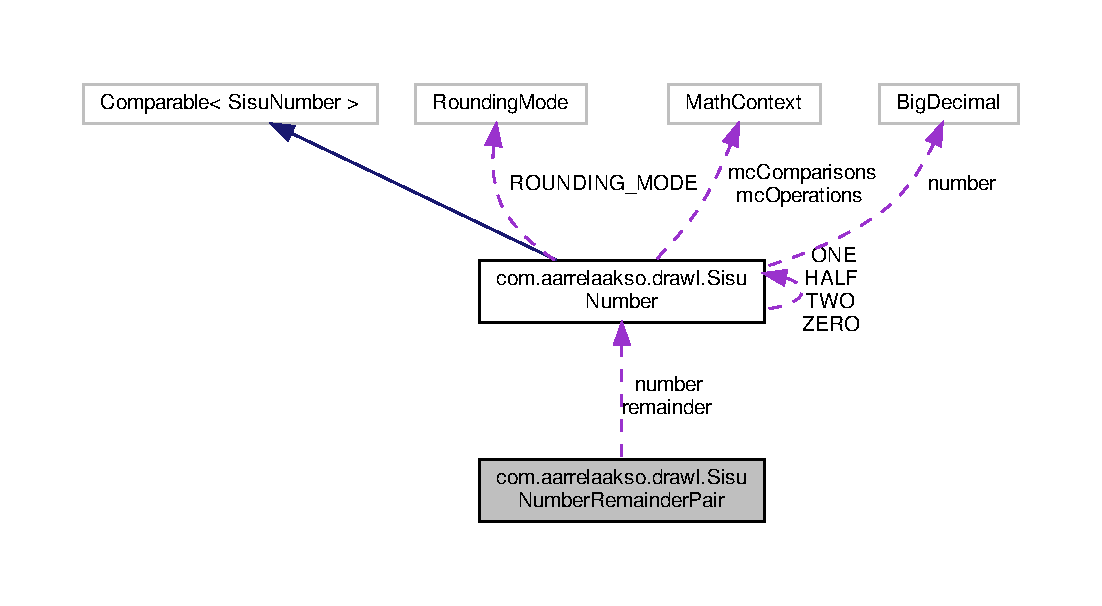
\includegraphics[width=350pt]{d3/d6a/classcom_1_1aarrelaakso_1_1drawl_1_1_sisu_number_remainder_pair__coll__graph}
\end{center}
\end{figure}
\subsection*{Public Member Functions}
\begin{DoxyCompactItemize}
\item 
boolean \hyperlink{classcom_1_1aarrelaakso_1_1drawl_1_1_sisu_number_remainder_pair_ad019d3d5cbc76e6e66b92f6e7aed6794}{equals} (final Object obj)
\item 
\hyperlink{classcom_1_1aarrelaakso_1_1drawl_1_1_sisu_number}{Sisu\+Number} \hyperlink{classcom_1_1aarrelaakso_1_1drawl_1_1_sisu_number_remainder_pair_a0811842d4cf4746c09c81fca090f98e1}{get\+Number} ()
\begin{DoxyCompactList}\small\item\em Returns number. \end{DoxyCompactList}\item 
\hyperlink{classcom_1_1aarrelaakso_1_1drawl_1_1_sisu_number}{Sisu\+Number} \hyperlink{classcom_1_1aarrelaakso_1_1drawl_1_1_sisu_number_remainder_pair_a2fb5bd3f444211337da3ce927b821c56}{get\+Remainder} ()
\begin{DoxyCompactList}\small\item\em Returns remainder. \end{DoxyCompactList}\item 
int \hyperlink{classcom_1_1aarrelaakso_1_1drawl_1_1_sisu_number_remainder_pair_a1cb5209ed6a95a1337fea5f4c9709b33}{hash\+Code} ()
\item 
String \hyperlink{classcom_1_1aarrelaakso_1_1drawl_1_1_sisu_number_remainder_pair_a0468d2a2b1f5db91a39390dbc18de7a8}{to\+String} ()
\end{DoxyCompactItemize}
\subsection*{Static Public Member Functions}
\begin{DoxyCompactItemize}
\item 
static \hyperlink{classcom_1_1aarrelaakso_1_1drawl_1_1_sisu_number_remainder_pair}{Sisu\+Number\+Remainder\+Pair} \hyperlink{classcom_1_1aarrelaakso_1_1drawl_1_1_sisu_number_remainder_pair_aa489b0cd18117d9c7d4994ec60af0984}{value\+Of} (final \hyperlink{classcom_1_1aarrelaakso_1_1drawl_1_1_sisu_number}{Sisu\+Number} \hyperlink{classcom_1_1aarrelaakso_1_1drawl_1_1_sisu_number_remainder_pair_a7ff7c95e41cb9dfbccb419fc75d05706}{number}, final \hyperlink{classcom_1_1aarrelaakso_1_1drawl_1_1_sisu_number}{Sisu\+Number} \hyperlink{classcom_1_1aarrelaakso_1_1drawl_1_1_sisu_number_remainder_pair_a2db9bc3ff60d0078b3341f75dd830890}{remainder})
\begin{DoxyCompactList}\small\item\em Creates new instance. \end{DoxyCompactList}\end{DoxyCompactItemize}
\subsection*{Private Member Functions}
\begin{DoxyCompactItemize}
\item 
\hyperlink{classcom_1_1aarrelaakso_1_1drawl_1_1_sisu_number_remainder_pair_adc48547d9eb6d9b59734cda97198e37c}{Sisu\+Number\+Remainder\+Pair} ()
\begin{DoxyCompactList}\small\item\em Creates new instance. \end{DoxyCompactList}\item 
void \hyperlink{classcom_1_1aarrelaakso_1_1drawl_1_1_sisu_number_remainder_pair_ac1a84d348f25642a02cae7df8903119c}{guard\+Invariants} ()
\begin{DoxyCompactList}\small\item\em Guards this object to be consistent. \end{DoxyCompactList}\end{DoxyCompactItemize}
\subsection*{Private Attributes}
\begin{DoxyCompactItemize}
\item 
\hyperlink{classcom_1_1aarrelaakso_1_1drawl_1_1_sisu_number}{Sisu\+Number} \hyperlink{classcom_1_1aarrelaakso_1_1drawl_1_1_sisu_number_remainder_pair_a7ff7c95e41cb9dfbccb419fc75d05706}{number}
\begin{DoxyCompactList}\small\item\em Unit number. \end{DoxyCompactList}\item 
\hyperlink{classcom_1_1aarrelaakso_1_1drawl_1_1_sisu_number}{Sisu\+Number} \hyperlink{classcom_1_1aarrelaakso_1_1drawl_1_1_sisu_number_remainder_pair_a2db9bc3ff60d0078b3341f75dd830890}{remainder}
\begin{DoxyCompactList}\small\item\em Remainder. \end{DoxyCompactList}\end{DoxyCompactItemize}


\subsection{Detailed Description}
Pair of the arbitrary number and remainder. 

This is the result after division operation.

\begin{DoxyAuthor}{Author}
radek.\+hecl 
\end{DoxyAuthor}


\subsection{Constructor \& Destructor Documentation}
\mbox{\Hypertarget{classcom_1_1aarrelaakso_1_1drawl_1_1_sisu_number_remainder_pair_adc48547d9eb6d9b59734cda97198e37c}\label{classcom_1_1aarrelaakso_1_1drawl_1_1_sisu_number_remainder_pair_adc48547d9eb6d9b59734cda97198e37c}} 
\index{com\+::aarrelaakso\+::drawl\+::\+Sisu\+Number\+Remainder\+Pair@{com\+::aarrelaakso\+::drawl\+::\+Sisu\+Number\+Remainder\+Pair}!Sisu\+Number\+Remainder\+Pair@{Sisu\+Number\+Remainder\+Pair}}
\index{Sisu\+Number\+Remainder\+Pair@{Sisu\+Number\+Remainder\+Pair}!com\+::aarrelaakso\+::drawl\+::\+Sisu\+Number\+Remainder\+Pair@{com\+::aarrelaakso\+::drawl\+::\+Sisu\+Number\+Remainder\+Pair}}
\subsubsection{\texorpdfstring{Sisu\+Number\+Remainder\+Pair()}{SisuNumberRemainderPair()}}
{\footnotesize\ttfamily com.\+aarrelaakso.\+drawl.\+Sisu\+Number\+Remainder\+Pair.\+Sisu\+Number\+Remainder\+Pair (\begin{DoxyParamCaption}{ }\end{DoxyParamCaption})\hspace{0.3cm}{\ttfamily [private]}}



Creates new instance. 



\subsection{Member Function Documentation}
\mbox{\Hypertarget{classcom_1_1aarrelaakso_1_1drawl_1_1_sisu_number_remainder_pair_ad019d3d5cbc76e6e66b92f6e7aed6794}\label{classcom_1_1aarrelaakso_1_1drawl_1_1_sisu_number_remainder_pair_ad019d3d5cbc76e6e66b92f6e7aed6794}} 
\index{com\+::aarrelaakso\+::drawl\+::\+Sisu\+Number\+Remainder\+Pair@{com\+::aarrelaakso\+::drawl\+::\+Sisu\+Number\+Remainder\+Pair}!equals@{equals}}
\index{equals@{equals}!com\+::aarrelaakso\+::drawl\+::\+Sisu\+Number\+Remainder\+Pair@{com\+::aarrelaakso\+::drawl\+::\+Sisu\+Number\+Remainder\+Pair}}
\subsubsection{\texorpdfstring{equals()}{equals()}}
{\footnotesize\ttfamily boolean com.\+aarrelaakso.\+drawl.\+Sisu\+Number\+Remainder\+Pair.\+equals (\begin{DoxyParamCaption}\item[{final Object}]{obj }\end{DoxyParamCaption})}

\mbox{\Hypertarget{classcom_1_1aarrelaakso_1_1drawl_1_1_sisu_number_remainder_pair_a0811842d4cf4746c09c81fca090f98e1}\label{classcom_1_1aarrelaakso_1_1drawl_1_1_sisu_number_remainder_pair_a0811842d4cf4746c09c81fca090f98e1}} 
\index{com\+::aarrelaakso\+::drawl\+::\+Sisu\+Number\+Remainder\+Pair@{com\+::aarrelaakso\+::drawl\+::\+Sisu\+Number\+Remainder\+Pair}!get\+Number@{get\+Number}}
\index{get\+Number@{get\+Number}!com\+::aarrelaakso\+::drawl\+::\+Sisu\+Number\+Remainder\+Pair@{com\+::aarrelaakso\+::drawl\+::\+Sisu\+Number\+Remainder\+Pair}}
\subsubsection{\texorpdfstring{get\+Number()}{getNumber()}}
{\footnotesize\ttfamily \hyperlink{classcom_1_1aarrelaakso_1_1drawl_1_1_sisu_number}{Sisu\+Number} com.\+aarrelaakso.\+drawl.\+Sisu\+Number\+Remainder\+Pair.\+get\+Number (\begin{DoxyParamCaption}{ }\end{DoxyParamCaption})}



Returns number. 

\begin{DoxyReturn}{Returns}
number 
\end{DoxyReturn}
\mbox{\Hypertarget{classcom_1_1aarrelaakso_1_1drawl_1_1_sisu_number_remainder_pair_a2fb5bd3f444211337da3ce927b821c56}\label{classcom_1_1aarrelaakso_1_1drawl_1_1_sisu_number_remainder_pair_a2fb5bd3f444211337da3ce927b821c56}} 
\index{com\+::aarrelaakso\+::drawl\+::\+Sisu\+Number\+Remainder\+Pair@{com\+::aarrelaakso\+::drawl\+::\+Sisu\+Number\+Remainder\+Pair}!get\+Remainder@{get\+Remainder}}
\index{get\+Remainder@{get\+Remainder}!com\+::aarrelaakso\+::drawl\+::\+Sisu\+Number\+Remainder\+Pair@{com\+::aarrelaakso\+::drawl\+::\+Sisu\+Number\+Remainder\+Pair}}
\subsubsection{\texorpdfstring{get\+Remainder()}{getRemainder()}}
{\footnotesize\ttfamily \hyperlink{classcom_1_1aarrelaakso_1_1drawl_1_1_sisu_number}{Sisu\+Number} com.\+aarrelaakso.\+drawl.\+Sisu\+Number\+Remainder\+Pair.\+get\+Remainder (\begin{DoxyParamCaption}{ }\end{DoxyParamCaption})}



Returns remainder. 

\begin{DoxyReturn}{Returns}
remainder 
\end{DoxyReturn}
\mbox{\Hypertarget{classcom_1_1aarrelaakso_1_1drawl_1_1_sisu_number_remainder_pair_ac1a84d348f25642a02cae7df8903119c}\label{classcom_1_1aarrelaakso_1_1drawl_1_1_sisu_number_remainder_pair_ac1a84d348f25642a02cae7df8903119c}} 
\index{com\+::aarrelaakso\+::drawl\+::\+Sisu\+Number\+Remainder\+Pair@{com\+::aarrelaakso\+::drawl\+::\+Sisu\+Number\+Remainder\+Pair}!guard\+Invariants@{guard\+Invariants}}
\index{guard\+Invariants@{guard\+Invariants}!com\+::aarrelaakso\+::drawl\+::\+Sisu\+Number\+Remainder\+Pair@{com\+::aarrelaakso\+::drawl\+::\+Sisu\+Number\+Remainder\+Pair}}
\subsubsection{\texorpdfstring{guard\+Invariants()}{guardInvariants()}}
{\footnotesize\ttfamily void com.\+aarrelaakso.\+drawl.\+Sisu\+Number\+Remainder\+Pair.\+guard\+Invariants (\begin{DoxyParamCaption}{ }\end{DoxyParamCaption})\hspace{0.3cm}{\ttfamily [private]}}



Guards this object to be consistent. 

Throws exception if this is not the case. \mbox{\Hypertarget{classcom_1_1aarrelaakso_1_1drawl_1_1_sisu_number_remainder_pair_a1cb5209ed6a95a1337fea5f4c9709b33}\label{classcom_1_1aarrelaakso_1_1drawl_1_1_sisu_number_remainder_pair_a1cb5209ed6a95a1337fea5f4c9709b33}} 
\index{com\+::aarrelaakso\+::drawl\+::\+Sisu\+Number\+Remainder\+Pair@{com\+::aarrelaakso\+::drawl\+::\+Sisu\+Number\+Remainder\+Pair}!hash\+Code@{hash\+Code}}
\index{hash\+Code@{hash\+Code}!com\+::aarrelaakso\+::drawl\+::\+Sisu\+Number\+Remainder\+Pair@{com\+::aarrelaakso\+::drawl\+::\+Sisu\+Number\+Remainder\+Pair}}
\subsubsection{\texorpdfstring{hash\+Code()}{hashCode()}}
{\footnotesize\ttfamily int com.\+aarrelaakso.\+drawl.\+Sisu\+Number\+Remainder\+Pair.\+hash\+Code (\begin{DoxyParamCaption}{ }\end{DoxyParamCaption})}

\mbox{\Hypertarget{classcom_1_1aarrelaakso_1_1drawl_1_1_sisu_number_remainder_pair_a0468d2a2b1f5db91a39390dbc18de7a8}\label{classcom_1_1aarrelaakso_1_1drawl_1_1_sisu_number_remainder_pair_a0468d2a2b1f5db91a39390dbc18de7a8}} 
\index{com\+::aarrelaakso\+::drawl\+::\+Sisu\+Number\+Remainder\+Pair@{com\+::aarrelaakso\+::drawl\+::\+Sisu\+Number\+Remainder\+Pair}!to\+String@{to\+String}}
\index{to\+String@{to\+String}!com\+::aarrelaakso\+::drawl\+::\+Sisu\+Number\+Remainder\+Pair@{com\+::aarrelaakso\+::drawl\+::\+Sisu\+Number\+Remainder\+Pair}}
\subsubsection{\texorpdfstring{to\+String()}{toString()}}
{\footnotesize\ttfamily String com.\+aarrelaakso.\+drawl.\+Sisu\+Number\+Remainder\+Pair.\+to\+String (\begin{DoxyParamCaption}{ }\end{DoxyParamCaption})}

\mbox{\Hypertarget{classcom_1_1aarrelaakso_1_1drawl_1_1_sisu_number_remainder_pair_aa489b0cd18117d9c7d4994ec60af0984}\label{classcom_1_1aarrelaakso_1_1drawl_1_1_sisu_number_remainder_pair_aa489b0cd18117d9c7d4994ec60af0984}} 
\index{com\+::aarrelaakso\+::drawl\+::\+Sisu\+Number\+Remainder\+Pair@{com\+::aarrelaakso\+::drawl\+::\+Sisu\+Number\+Remainder\+Pair}!value\+Of@{value\+Of}}
\index{value\+Of@{value\+Of}!com\+::aarrelaakso\+::drawl\+::\+Sisu\+Number\+Remainder\+Pair@{com\+::aarrelaakso\+::drawl\+::\+Sisu\+Number\+Remainder\+Pair}}
\subsubsection{\texorpdfstring{value\+Of()}{valueOf()}}
{\footnotesize\ttfamily static \hyperlink{classcom_1_1aarrelaakso_1_1drawl_1_1_sisu_number_remainder_pair}{Sisu\+Number\+Remainder\+Pair} com.\+aarrelaakso.\+drawl.\+Sisu\+Number\+Remainder\+Pair.\+value\+Of (\begin{DoxyParamCaption}\item[{final \hyperlink{classcom_1_1aarrelaakso_1_1drawl_1_1_sisu_number}{Sisu\+Number}}]{number,  }\item[{final \hyperlink{classcom_1_1aarrelaakso_1_1drawl_1_1_sisu_number}{Sisu\+Number}}]{remainder }\end{DoxyParamCaption})\hspace{0.3cm}{\ttfamily [static]}}



Creates new instance. 


\begin{DoxyParams}{Parameters}
{\em number} & number \\
\hline
{\em remainder} & remainder \\
\hline
\end{DoxyParams}
\begin{DoxyReturn}{Returns}
number remainder pair 
\end{DoxyReturn}


\subsection{Member Data Documentation}
\mbox{\Hypertarget{classcom_1_1aarrelaakso_1_1drawl_1_1_sisu_number_remainder_pair_a7ff7c95e41cb9dfbccb419fc75d05706}\label{classcom_1_1aarrelaakso_1_1drawl_1_1_sisu_number_remainder_pair_a7ff7c95e41cb9dfbccb419fc75d05706}} 
\index{com\+::aarrelaakso\+::drawl\+::\+Sisu\+Number\+Remainder\+Pair@{com\+::aarrelaakso\+::drawl\+::\+Sisu\+Number\+Remainder\+Pair}!number@{number}}
\index{number@{number}!com\+::aarrelaakso\+::drawl\+::\+Sisu\+Number\+Remainder\+Pair@{com\+::aarrelaakso\+::drawl\+::\+Sisu\+Number\+Remainder\+Pair}}
\subsubsection{\texorpdfstring{number}{number}}
{\footnotesize\ttfamily \hyperlink{classcom_1_1aarrelaakso_1_1drawl_1_1_sisu_number}{Sisu\+Number} com.\+aarrelaakso.\+drawl.\+Sisu\+Number\+Remainder\+Pair.\+number\hspace{0.3cm}{\ttfamily [private]}}



Unit number. 

\mbox{\Hypertarget{classcom_1_1aarrelaakso_1_1drawl_1_1_sisu_number_remainder_pair_a2db9bc3ff60d0078b3341f75dd830890}\label{classcom_1_1aarrelaakso_1_1drawl_1_1_sisu_number_remainder_pair_a2db9bc3ff60d0078b3341f75dd830890}} 
\index{com\+::aarrelaakso\+::drawl\+::\+Sisu\+Number\+Remainder\+Pair@{com\+::aarrelaakso\+::drawl\+::\+Sisu\+Number\+Remainder\+Pair}!remainder@{remainder}}
\index{remainder@{remainder}!com\+::aarrelaakso\+::drawl\+::\+Sisu\+Number\+Remainder\+Pair@{com\+::aarrelaakso\+::drawl\+::\+Sisu\+Number\+Remainder\+Pair}}
\subsubsection{\texorpdfstring{remainder}{remainder}}
{\footnotesize\ttfamily \hyperlink{classcom_1_1aarrelaakso_1_1drawl_1_1_sisu_number}{Sisu\+Number} com.\+aarrelaakso.\+drawl.\+Sisu\+Number\+Remainder\+Pair.\+remainder\hspace{0.3cm}{\ttfamily [private]}}



Remainder. 



The documentation for this class was generated from the following file\+:\begin{DoxyCompactItemize}
\item 
/mnt/d/\+One\+Drive/\+Documents/src/drawl/src/main/java/com/aarrelaakso/drawl/\hyperlink{_sisu_number_remainder_pair_8java}{Sisu\+Number\+Remainder\+Pair.\+java}\end{DoxyCompactItemize}

\hypertarget{classcom_1_1aarrelaakso_1_1drawl_1_1_s_v_g}{}\section{com.\+aarrelaakso.\+drawl.\+S\+VG Class Reference}
\label{classcom_1_1aarrelaakso_1_1drawl_1_1_s_v_g}\index{com.\+aarrelaakso.\+drawl.\+S\+VG@{com.\+aarrelaakso.\+drawl.\+S\+VG}}
\subsection*{Static Public Member Functions}
\begin{DoxyCompactItemize}
\item 
static String \hyperlink{classcom_1_1aarrelaakso_1_1drawl_1_1_s_v_g_ae360f344b090fed4452294dbf980185d}{to\+String} (\hyperlink{classcom_1_1aarrelaakso_1_1drawl_1_1_drawl_number}{Drawl\+Number} number)
\begin{DoxyCompactList}\small\item\em Convert a number to a string for \hyperlink{classcom_1_1aarrelaakso_1_1drawl_1_1_s_v_g}{S\+VG}. \end{DoxyCompactList}\end{DoxyCompactItemize}


\subsection{Member Function Documentation}
\mbox{\Hypertarget{classcom_1_1aarrelaakso_1_1drawl_1_1_s_v_g_ae360f344b090fed4452294dbf980185d}\label{classcom_1_1aarrelaakso_1_1drawl_1_1_s_v_g_ae360f344b090fed4452294dbf980185d}} 
\index{com\+::aarrelaakso\+::drawl\+::\+S\+VG@{com\+::aarrelaakso\+::drawl\+::\+S\+VG}!to\+String@{to\+String}}
\index{to\+String@{to\+String}!com\+::aarrelaakso\+::drawl\+::\+S\+VG@{com\+::aarrelaakso\+::drawl\+::\+S\+VG}}
\subsubsection{\texorpdfstring{to\+String()}{toString()}}
{\footnotesize\ttfamily static String com.\+aarrelaakso.\+drawl.\+S\+V\+G.\+to\+String (\begin{DoxyParamCaption}\item[{\hyperlink{classcom_1_1aarrelaakso_1_1drawl_1_1_drawl_number}{Drawl\+Number}}]{number }\end{DoxyParamCaption})\hspace{0.3cm}{\ttfamily [static]}}



Convert a number to a string for \hyperlink{classcom_1_1aarrelaakso_1_1drawl_1_1_s_v_g}{S\+VG}. 

The number will be represented with as many decimal points as necessary for \hyperlink{classcom_1_1aarrelaakso_1_1drawl_1_1_s_v_g}{S\+VG} and no more than \hyperlink{classcom_1_1aarrelaakso_1_1drawl_1_1_s_v_g}{S\+VG} can handle.


\begin{DoxyParams}{Parameters}
{\em number} & the number to convert. \\
\hline
\end{DoxyParams}


The documentation for this class was generated from the following file\+:\begin{DoxyCompactItemize}
\item 
/mnt/d/\+One\+Drive/\+Documents/src/drawl/src/main/java/com/aarrelaakso/drawl/\hyperlink{_s_v_g_8java}{S\+V\+G.\+java}\end{DoxyCompactItemize}

\hypertarget{classcom_1_1aarrelaakso_1_1drawl_1_1_text}{}\section{com.\+aarrelaakso.\+drawl.\+Text Class Reference}
\label{classcom_1_1aarrelaakso_1_1drawl_1_1_text}\index{com.\+aarrelaakso.\+drawl.\+Text@{com.\+aarrelaakso.\+drawl.\+Text}}


Represents text on a drawing.  




Inheritance diagram for com.\+aarrelaakso.\+drawl.\+Text\+:\nopagebreak
\begin{figure}[H]
\begin{center}
\leavevmode
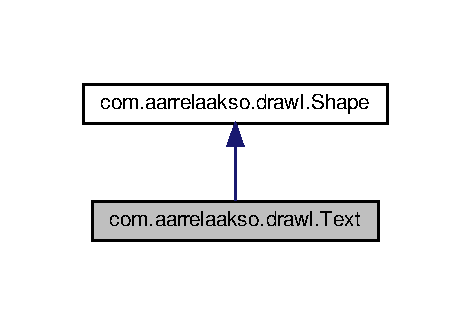
\includegraphics[width=226pt]{dd/dcf/classcom_1_1aarrelaakso_1_1drawl_1_1_text__inherit__graph}
\end{center}
\end{figure}


Collaboration diagram for com.\+aarrelaakso.\+drawl.\+Text\+:\nopagebreak
\begin{figure}[H]
\begin{center}
\leavevmode
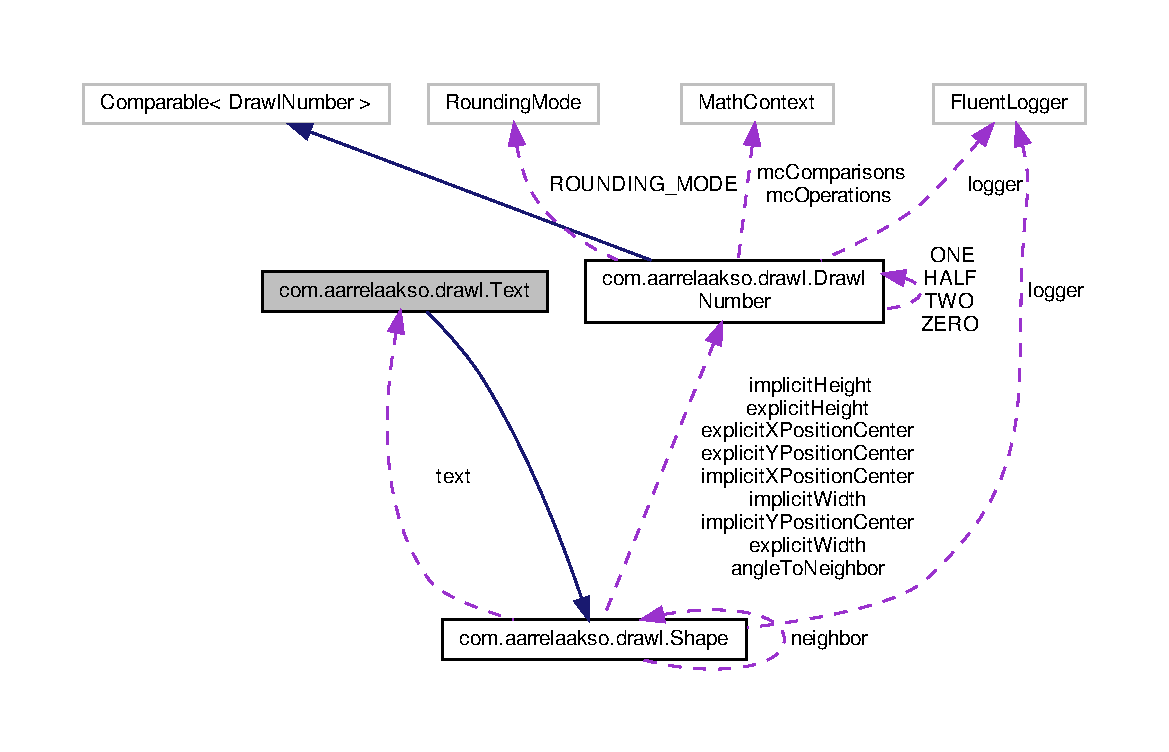
\includegraphics[width=350pt]{df/d69/classcom_1_1aarrelaakso_1_1drawl_1_1_text__coll__graph}
\end{center}
\end{figure}
\subsection*{Public Member Functions}
\begin{DoxyCompactItemize}
\item 
\hyperlink{classcom_1_1aarrelaakso_1_1drawl_1_1_text_a9d9bdd3df91ff551c7bf96f741cde0e9}{Text} ()
\begin{DoxyCompactList}\small\item\em Constructs a default \hyperlink{classcom_1_1aarrelaakso_1_1drawl_1_1_text}{Text} object. \end{DoxyCompactList}\item 
\hyperlink{classcom_1_1aarrelaakso_1_1drawl_1_1_text_a8a30634e847c9c235c97aa3c20f991b7}{Text} (@Not\+Null final String \hyperlink{classcom_1_1aarrelaakso_1_1drawl_1_1_text_a94bf15b06c72349f5d5a1bfc56496685}{string})
\begin{DoxyCompactList}\small\item\em Constructs a \hyperlink{classcom_1_1aarrelaakso_1_1drawl_1_1_text}{Text} object with some text. \end{DoxyCompactList}\item 
String \hyperlink{classcom_1_1aarrelaakso_1_1drawl_1_1_text_ab1a6091b007ea4da41de26bc8c6ea021}{get\+S\+VG} ()
\begin{DoxyCompactList}\small\item\em Gets the \hyperlink{classcom_1_1aarrelaakso_1_1drawl_1_1_s_v_g}{S\+VG} associated with this \hyperlink{classcom_1_1aarrelaakso_1_1drawl_1_1_text}{Text} object. \end{DoxyCompactList}\item 
void \hyperlink{classcom_1_1aarrelaakso_1_1drawl_1_1_text_a8fec7a478b7a7f4a141e36ee52a66a42}{set\+String} (@Nullable final String \hyperlink{classcom_1_1aarrelaakso_1_1drawl_1_1_text_a94bf15b06c72349f5d5a1bfc56496685}{string})
\begin{DoxyCompactList}\small\item\em Sets the string associated with this \hyperlink{classcom_1_1aarrelaakso_1_1drawl_1_1_text}{Text} object. \end{DoxyCompactList}\item 
String \hyperlink{classcom_1_1aarrelaakso_1_1drawl_1_1_text_aaded65428b035e05b91e65f21808b434}{to\+String} ()
\begin{DoxyCompactList}\small\item\em Gets the text string associated with this \hyperlink{classcom_1_1aarrelaakso_1_1drawl_1_1_text}{Text} object. \end{DoxyCompactList}\item 
void \hyperlink{classcom_1_1aarrelaakso_1_1drawl_1_1_shape_af6fea9610721de462c18ee640043aba7}{add\+Text} (@Nullable final \hyperlink{classcom_1_1aarrelaakso_1_1drawl_1_1_text}{Text} \hyperlink{classcom_1_1aarrelaakso_1_1drawl_1_1_shape_ab54afc2d95d3447532f5ecf3fec3faa8}{text})
\begin{DoxyCompactList}\small\item\em Adds \hyperlink{classcom_1_1aarrelaakso_1_1drawl_1_1_text}{Text} inside this \hyperlink{classcom_1_1aarrelaakso_1_1drawl_1_1_shape}{Shape}. \end{DoxyCompactList}\item 
\hyperlink{classcom_1_1aarrelaakso_1_1drawl_1_1_shape}{Shape} \hyperlink{classcom_1_1aarrelaakso_1_1drawl_1_1_shape_acebea2aa57031322323c9bf50ee447db}{get\+Above} ()
\begin{DoxyCompactList}\small\item\em Gets this \hyperlink{classcom_1_1aarrelaakso_1_1drawl_1_1_shape}{Shape}\textquotesingle{}s neighbor above (this \hyperlink{classcom_1_1aarrelaakso_1_1drawl_1_1_shape}{Shape} is below that one), if any. \end{DoxyCompactList}\item 
void \hyperlink{classcom_1_1aarrelaakso_1_1drawl_1_1_shape_a4deb22d64fef2115a0bc4802e8dba682}{set\+Above} (@Not\+Null final \hyperlink{classcom_1_1aarrelaakso_1_1drawl_1_1_shape}{Shape} shape)
\begin{DoxyCompactList}\small\item\em Sets this \hyperlink{classcom_1_1aarrelaakso_1_1drawl_1_1_shape}{Shape} above another \hyperlink{classcom_1_1aarrelaakso_1_1drawl_1_1_shape}{Shape}. \end{DoxyCompactList}\item 
void \hyperlink{classcom_1_1aarrelaakso_1_1drawl_1_1_shape_aad0b2fb173c0112b71b06cf90709acc3}{set\+Above} (@Not\+Null final \hyperlink{classcom_1_1aarrelaakso_1_1drawl_1_1_shape}{Shape} shape, @Not\+Null final \hyperlink{classcom_1_1aarrelaakso_1_1drawl_1_1_measure}{Measure} offset)
\begin{DoxyCompactList}\small\item\em Sets this \hyperlink{classcom_1_1aarrelaakso_1_1drawl_1_1_shape}{Shape} above another \hyperlink{classcom_1_1aarrelaakso_1_1drawl_1_1_shape}{Shape}. \end{DoxyCompactList}\item 
\hyperlink{classcom_1_1aarrelaakso_1_1drawl_1_1_shape}{Shape} \hyperlink{classcom_1_1aarrelaakso_1_1drawl_1_1_shape_a53de5ab609d879719cd3b372dfe8df58}{get\+Below} ()
\begin{DoxyCompactList}\small\item\em Gets this \hyperlink{classcom_1_1aarrelaakso_1_1drawl_1_1_shape}{Shape}\textquotesingle{}s neighbor below (this \hyperlink{classcom_1_1aarrelaakso_1_1drawl_1_1_shape}{Shape} is above that one), if any. \end{DoxyCompactList}\item 
void \hyperlink{classcom_1_1aarrelaakso_1_1drawl_1_1_shape_a4147526667449f5beb534d4404ba8f77}{set\+Below} (@Not\+Null final \hyperlink{classcom_1_1aarrelaakso_1_1drawl_1_1_shape}{Shape} shape)
\begin{DoxyCompactList}\small\item\em Sets this \hyperlink{classcom_1_1aarrelaakso_1_1drawl_1_1_shape}{Shape} below another \hyperlink{classcom_1_1aarrelaakso_1_1drawl_1_1_shape}{Shape}. \end{DoxyCompactList}\item 
void \hyperlink{classcom_1_1aarrelaakso_1_1drawl_1_1_shape_a63c902c4e79235901744c6d83544fa54}{set\+Below} (@Not\+Null final \hyperlink{classcom_1_1aarrelaakso_1_1drawl_1_1_shape}{Shape} shape, @Not\+Null final \hyperlink{classcom_1_1aarrelaakso_1_1drawl_1_1_measure}{Measure} offset)
\begin{DoxyCompactList}\small\item\em Sets this circle below another circle. \end{DoxyCompactList}\item 
\hyperlink{classcom_1_1aarrelaakso_1_1drawl_1_1_point}{Point} \hyperlink{classcom_1_1aarrelaakso_1_1drawl_1_1_shape_aba14efe9a16c0808580963c66b171082}{get\+Bottom\+Port} ()
\begin{DoxyCompactList}\small\item\em Returns a \hyperlink{classcom_1_1aarrelaakso_1_1drawl_1_1_point}{Point} object representing this \hyperlink{classcom_1_1aarrelaakso_1_1drawl_1_1_shape}{Shape}\textquotesingle{}s bottom port. \end{DoxyCompactList}\item 
String \hyperlink{classcom_1_1aarrelaakso_1_1drawl_1_1_shape_a0d9a33a3e151aaceeec140bea343a650}{get\+Fill} ()
\begin{DoxyCompactList}\small\item\em Returns the fill associated with this \hyperlink{classcom_1_1aarrelaakso_1_1drawl_1_1_shape}{Shape}, if any. \end{DoxyCompactList}\item 
void \hyperlink{classcom_1_1aarrelaakso_1_1drawl_1_1_shape_a81ff4feb49b8f74c1a639564748a23ee}{set\+Fill} (final String s)
\begin{DoxyCompactList}\small\item\em Set the fill of this \hyperlink{classcom_1_1aarrelaakso_1_1drawl_1_1_shape}{Shape}. \end{DoxyCompactList}\item 
\hyperlink{classcom_1_1aarrelaakso_1_1drawl_1_1_measure}{Measure} \hyperlink{classcom_1_1aarrelaakso_1_1drawl_1_1_shape_ac9f74d31c332aab76b329edc22080e67}{get\+Height} ()
\begin{DoxyCompactList}\small\item\em Returns a \hyperlink{classcom_1_1aarrelaakso_1_1drawl_1_1_measure}{Measure} object that represents the height of this \hyperlink{classcom_1_1aarrelaakso_1_1drawl_1_1_shape}{Shape}. \end{DoxyCompactList}\item 
\hyperlink{classcom_1_1aarrelaakso_1_1drawl_1_1_shape}{Shape} \hyperlink{classcom_1_1aarrelaakso_1_1drawl_1_1_shape_a2b19d5964ac46d545a7bae3133df6532}{get\+Left\+Of} ()
\begin{DoxyCompactList}\small\item\em Gets this \hyperlink{classcom_1_1aarrelaakso_1_1drawl_1_1_shape}{Shape}\textquotesingle{}s neighbor to the right (this \hyperlink{classcom_1_1aarrelaakso_1_1drawl_1_1_shape}{Shape} is to the left of that one), if any. \end{DoxyCompactList}\item 
void \hyperlink{classcom_1_1aarrelaakso_1_1drawl_1_1_shape_a0aef56392d76202235a9520394e87492}{set\+Left\+Of} (@Not\+Null final \hyperlink{classcom_1_1aarrelaakso_1_1drawl_1_1_shape}{Shape} shape)
\begin{DoxyCompactList}\small\item\em Sets this \hyperlink{classcom_1_1aarrelaakso_1_1drawl_1_1_shape}{Shape} to the left of another one. \end{DoxyCompactList}\item 
void \hyperlink{classcom_1_1aarrelaakso_1_1drawl_1_1_shape_a8012a3823982d77b563ef61787ccb523}{set\+Left\+Of} (@Not\+Null final \hyperlink{classcom_1_1aarrelaakso_1_1drawl_1_1_shape}{Shape} shape, @Not\+Null final \hyperlink{classcom_1_1aarrelaakso_1_1drawl_1_1_measure}{Measure} offset)
\begin{DoxyCompactList}\small\item\em Sets this \hyperlink{classcom_1_1aarrelaakso_1_1drawl_1_1_shape}{Shape}\textquotesingle{}s neighbor to the right (this \hyperlink{classcom_1_1aarrelaakso_1_1drawl_1_1_shape}{Shape} is to the left of that one). \end{DoxyCompactList}\item 
\hyperlink{classcom_1_1aarrelaakso_1_1drawl_1_1_point}{Point} \hyperlink{classcom_1_1aarrelaakso_1_1drawl_1_1_shape_aeffa96786ca552adf46924ec77da9555}{get\+Left\+Port} ()
\begin{DoxyCompactList}\small\item\em Returns a \hyperlink{classcom_1_1aarrelaakso_1_1drawl_1_1_point}{Point} object representing this \hyperlink{classcom_1_1aarrelaakso_1_1drawl_1_1_shape}{Shape}\textquotesingle{}s left port. \end{DoxyCompactList}\item 
\hyperlink{classcom_1_1aarrelaakso_1_1drawl_1_1_shape}{Shape} \hyperlink{classcom_1_1aarrelaakso_1_1drawl_1_1_shape_a1ad573b06f341aa79f6a255a476ae6e4}{get\+Right\+Of} ()
\begin{DoxyCompactList}\small\item\em Gets this \hyperlink{classcom_1_1aarrelaakso_1_1drawl_1_1_shape}{Shape}\textquotesingle{}s neighbor to the left (this \hyperlink{classcom_1_1aarrelaakso_1_1drawl_1_1_shape}{Shape} is to the right of that one), if any. \end{DoxyCompactList}\item 
void \hyperlink{classcom_1_1aarrelaakso_1_1drawl_1_1_shape_a3cada5e03bd1552a79702d2945c7ed01}{set\+Right\+Of} (@Not\+Null final \hyperlink{classcom_1_1aarrelaakso_1_1drawl_1_1_shape}{Shape} shape)
\begin{DoxyCompactList}\small\item\em Sets this \hyperlink{classcom_1_1aarrelaakso_1_1drawl_1_1_shape}{Shape}\textquotesingle{}s neighbor to the left (this \hyperlink{classcom_1_1aarrelaakso_1_1drawl_1_1_shape}{Shape} is to the right of that one). \end{DoxyCompactList}\item 
void \hyperlink{classcom_1_1aarrelaakso_1_1drawl_1_1_shape_a89e85848d24dca0fa60ff68d169eef11}{set\+Right\+Of} (@Not\+Null final \hyperlink{classcom_1_1aarrelaakso_1_1drawl_1_1_shape}{Shape} shape, @Not\+Null final \hyperlink{classcom_1_1aarrelaakso_1_1drawl_1_1_measure}{Measure} offset)
\begin{DoxyCompactList}\small\item\em Sets this \hyperlink{classcom_1_1aarrelaakso_1_1drawl_1_1_shape}{Shape}\textquotesingle{}s neighbor to the left with an offset. \end{DoxyCompactList}\item 
\hyperlink{classcom_1_1aarrelaakso_1_1drawl_1_1_point}{Point} \hyperlink{classcom_1_1aarrelaakso_1_1drawl_1_1_shape_a319c78d425ec91e1aef1072a95e349ad}{get\+Right\+Port} ()
\begin{DoxyCompactList}\small\item\em Returns a \hyperlink{classcom_1_1aarrelaakso_1_1drawl_1_1_point}{Point} object representing this \hyperlink{classcom_1_1aarrelaakso_1_1drawl_1_1_shape}{Shape}\textquotesingle{}s left port. \end{DoxyCompactList}\item 
String \hyperlink{classcom_1_1aarrelaakso_1_1drawl_1_1_shape_a4e1d54c7e161e3af5053939ddefdf9e6}{get\+Stroke} ()
\begin{DoxyCompactList}\small\item\em Gets the stroke of this \hyperlink{classcom_1_1aarrelaakso_1_1drawl_1_1_shape}{Shape}. \end{DoxyCompactList}\item 
void \hyperlink{classcom_1_1aarrelaakso_1_1drawl_1_1_shape_a75685cbfea36858836df8e1fb4f8b821}{set\+Stroke} (final String s)
\begin{DoxyCompactList}\small\item\em Sets the stroke of this shape. \end{DoxyCompactList}\item 
\hyperlink{classcom_1_1aarrelaakso_1_1drawl_1_1_text}{Text} \hyperlink{classcom_1_1aarrelaakso_1_1drawl_1_1_shape_a6f876978d4102974fedc5b41c93c7b26}{get\+Text} ()
\begin{DoxyCompactList}\small\item\em Returns a \hyperlink{classcom_1_1aarrelaakso_1_1drawl_1_1_text}{Text} object that belongs to this \hyperlink{classcom_1_1aarrelaakso_1_1drawl_1_1_shape}{Shape}, if there is one. \end{DoxyCompactList}\item 
\hyperlink{classcom_1_1aarrelaakso_1_1drawl_1_1_point}{Point} \hyperlink{classcom_1_1aarrelaakso_1_1drawl_1_1_shape_aed4e9caa294aacc973b7a531a960e9e5}{get\+Top\+Port} ()
\begin{DoxyCompactList}\small\item\em Returns a \hyperlink{classcom_1_1aarrelaakso_1_1drawl_1_1_point}{Point} object representing this \hyperlink{classcom_1_1aarrelaakso_1_1drawl_1_1_shape}{Shape}\textquotesingle{}s top port. \end{DoxyCompactList}\item 
void \hyperlink{classcom_1_1aarrelaakso_1_1drawl_1_1_shape_a8b5f19ff40445c0cf8cad2688d7df810}{set\+Width} (\hyperlink{classcom_1_1aarrelaakso_1_1drawl_1_1_measure}{Measure} width)
\begin{DoxyCompactList}\small\item\em Sets the width of this object. \end{DoxyCompactList}\item 
\hyperlink{classcom_1_1aarrelaakso_1_1drawl_1_1_measure}{Measure} \hyperlink{classcom_1_1aarrelaakso_1_1drawl_1_1_shape_a3e2c58984f1bcbc2e9e86cf30868561e}{get\+Width} ()
\begin{DoxyCompactList}\small\item\em Returns a \hyperlink{classcom_1_1aarrelaakso_1_1drawl_1_1_measure}{Measure} object that represents the width of this \hyperlink{classcom_1_1aarrelaakso_1_1drawl_1_1_shape}{Shape}. \end{DoxyCompactList}\item 
Boolean \hyperlink{classcom_1_1aarrelaakso_1_1drawl_1_1_shape_a037a5515b2a6e1df1d1981aa5516e78e}{has\+Text} ()
\begin{DoxyCompactList}\small\item\em Indicates whether this shape has a \hyperlink{classcom_1_1aarrelaakso_1_1drawl_1_1_text}{Text} object associated with it. \end{DoxyCompactList}\end{DoxyCompactItemize}
\subsection*{Protected Member Functions}
\begin{DoxyCompactItemize}
\item 
\hyperlink{interfacecom_1_1aarrelaakso_1_1drawl_1_1_number}{Number} \hyperlink{classcom_1_1aarrelaakso_1_1drawl_1_1_shape_a3acdc2fd1944e2efacd0bfbb8aefe89b}{get\+Explicit\+Half\+Width} ()
\begin{DoxyCompactList}\small\item\em Gets half the explicit width of this \hyperlink{classcom_1_1aarrelaakso_1_1drawl_1_1_shape}{Shape}. \end{DoxyCompactList}\item 
\hyperlink{interfacecom_1_1aarrelaakso_1_1drawl_1_1_number}{Number} \hyperlink{classcom_1_1aarrelaakso_1_1drawl_1_1_shape_a48917787cedbfd447cd37edbb59a1145}{get\+Explicit\+Height} ()
\begin{DoxyCompactList}\small\item\em Get the explicit height of this \hyperlink{classcom_1_1aarrelaakso_1_1drawl_1_1_shape}{Shape}. \end{DoxyCompactList}\item 
void \hyperlink{classcom_1_1aarrelaakso_1_1drawl_1_1_shape_a3680a63cef0d766132d1f64813ca8eca}{set\+Explicit\+Height} (@Nullable final \hyperlink{interfacecom_1_1aarrelaakso_1_1drawl_1_1_number}{Number} height)
\begin{DoxyCompactList}\small\item\em Set the height of this \hyperlink{classcom_1_1aarrelaakso_1_1drawl_1_1_shape}{Shape} to an explicit value. \end{DoxyCompactList}\item 
\hyperlink{interfacecom_1_1aarrelaakso_1_1drawl_1_1_number}{Number} \hyperlink{classcom_1_1aarrelaakso_1_1drawl_1_1_shape_aca08f18bbe102a5cf6a77cb746d42875}{get\+Explicit\+Width} ()
\begin{DoxyCompactList}\small\item\em Get the explicit width of this \hyperlink{classcom_1_1aarrelaakso_1_1drawl_1_1_shape}{Shape}. \end{DoxyCompactList}\item 
void \hyperlink{classcom_1_1aarrelaakso_1_1drawl_1_1_shape_a386685477bfc007aab782565f140265d}{set\+Explicit\+Width} (@Nullable final \hyperlink{interfacecom_1_1aarrelaakso_1_1drawl_1_1_number}{Number} width)
\begin{DoxyCompactList}\small\item\em Set the width of this \hyperlink{classcom_1_1aarrelaakso_1_1drawl_1_1_shape}{Shape} to an explicit value. \end{DoxyCompactList}\item 
\hyperlink{interfacecom_1_1aarrelaakso_1_1drawl_1_1_number}{Number} \hyperlink{classcom_1_1aarrelaakso_1_1drawl_1_1_shape_aa1fbd5a290bc5d2df437f0bd79f30a89}{get\+Explicit\+X\+Position\+Center} ()
\begin{DoxyCompactList}\small\item\em Gets the explicit x-\/position of the center of this \hyperlink{classcom_1_1aarrelaakso_1_1drawl_1_1_shape}{Shape}. \end{DoxyCompactList}\item 
void \hyperlink{classcom_1_1aarrelaakso_1_1drawl_1_1_shape_a28c766b414be0cd8767093f9be557dbd}{set\+Explicit\+X\+Position\+Center} (final \hyperlink{interfacecom_1_1aarrelaakso_1_1drawl_1_1_number}{Number} x)
\begin{DoxyCompactList}\small\item\em Sets the explicit center position of this \hyperlink{classcom_1_1aarrelaakso_1_1drawl_1_1_shape}{Shape}. \end{DoxyCompactList}\item 
void \hyperlink{classcom_1_1aarrelaakso_1_1drawl_1_1_shape_a271cd9377952616a30a434b22e22000a}{set\+Explicit\+X\+Position\+Center} (final Integer x)
\begin{DoxyCompactList}\small\item\em Sets the explicit x position of the center of this \hyperlink{classcom_1_1aarrelaakso_1_1drawl_1_1_shape}{Shape}. \end{DoxyCompactList}\item 
\hyperlink{interfacecom_1_1aarrelaakso_1_1drawl_1_1_number}{Number} \hyperlink{classcom_1_1aarrelaakso_1_1drawl_1_1_shape_abd7f6c77e2c62100bb72d8ad3085e288}{get\+Explicit\+X\+Position\+Left} ()
\begin{DoxyCompactList}\small\item\em Gets the explicit x position of the left edge of this \hyperlink{classcom_1_1aarrelaakso_1_1drawl_1_1_shape}{Shape}. \end{DoxyCompactList}\item 
\hyperlink{interfacecom_1_1aarrelaakso_1_1drawl_1_1_number}{Number} \hyperlink{classcom_1_1aarrelaakso_1_1drawl_1_1_shape_a86920ba43a76d5a02977e5f9ea3509ac}{get\+Explicit\+X\+Position\+Right} ()
\begin{DoxyCompactList}\small\item\em Gets the explicit x position of the right edge of this \hyperlink{classcom_1_1aarrelaakso_1_1drawl_1_1_shape}{Shape}. \end{DoxyCompactList}\item 
\hyperlink{interfacecom_1_1aarrelaakso_1_1drawl_1_1_number}{Number} \hyperlink{classcom_1_1aarrelaakso_1_1drawl_1_1_shape_a28b8e03381be6afdc7c5c8da48c80afe}{get\+Explicit\+Y\+Position\+Bottom} ()
\begin{DoxyCompactList}\small\item\em Gets the explicit y position of the bottom of this \hyperlink{classcom_1_1aarrelaakso_1_1drawl_1_1_shape}{Shape}. \end{DoxyCompactList}\item 
\hyperlink{interfacecom_1_1aarrelaakso_1_1drawl_1_1_number}{Number} \hyperlink{classcom_1_1aarrelaakso_1_1drawl_1_1_shape_a1e46cc626d5f5e1360d9d35d23cc50ea}{get\+Explicit\+Y\+Position\+Center} ()
\begin{DoxyCompactList}\small\item\em Gets the explicit y-\/position of the center of this \hyperlink{classcom_1_1aarrelaakso_1_1drawl_1_1_shape}{Shape}. \end{DoxyCompactList}\item 
void \hyperlink{classcom_1_1aarrelaakso_1_1drawl_1_1_shape_a93e9e1bdd05f111661660e9de621cd12}{set\+Explicit\+Y\+Position\+Center} (final Integer y)
\begin{DoxyCompactList}\small\item\em Sets the explicit y-\/position of the center of this \hyperlink{classcom_1_1aarrelaakso_1_1drawl_1_1_shape}{Shape}. \end{DoxyCompactList}\item 
void \hyperlink{classcom_1_1aarrelaakso_1_1drawl_1_1_shape_a7d49d69bd74e57c3a3341a025c3cce50}{set\+Explicit\+Y\+Position\+Center} (final \hyperlink{interfacecom_1_1aarrelaakso_1_1drawl_1_1_number}{Number} y)
\begin{DoxyCompactList}\small\item\em Sets the explicit y position of this \hyperlink{classcom_1_1aarrelaakso_1_1drawl_1_1_shape}{Shape}. \end{DoxyCompactList}\item 
\hyperlink{interfacecom_1_1aarrelaakso_1_1drawl_1_1_number}{Number} \hyperlink{classcom_1_1aarrelaakso_1_1drawl_1_1_shape_a8c65dff2026744ae10648de3908165e5}{get\+Explicit\+Y\+Position\+Top} ()
\begin{DoxyCompactList}\small\item\em Gets the explicit y-\/position of the top of this \hyperlink{classcom_1_1aarrelaakso_1_1drawl_1_1_shape}{Shape}. \end{DoxyCompactList}\item 
\hyperlink{interfacecom_1_1aarrelaakso_1_1drawl_1_1_number}{Number} \hyperlink{classcom_1_1aarrelaakso_1_1drawl_1_1_shape_a4af0fd7e309ea01bced73076510ef897}{get\+Implicit\+Half\+Height} ()
\begin{DoxyCompactList}\small\item\em Gets half of the implicit height of this \hyperlink{classcom_1_1aarrelaakso_1_1drawl_1_1_shape}{Shape}. \end{DoxyCompactList}\item 
\hyperlink{interfacecom_1_1aarrelaakso_1_1drawl_1_1_number}{Number} \hyperlink{classcom_1_1aarrelaakso_1_1drawl_1_1_shape_a02d73887a309bcd1178b142ad0c7edd9}{get\+Implicit\+Half\+Width} ()
\begin{DoxyCompactList}\small\item\em Gets half of the implicit width of this \hyperlink{classcom_1_1aarrelaakso_1_1drawl_1_1_shape}{Shape}. \end{DoxyCompactList}\item 
\hyperlink{interfacecom_1_1aarrelaakso_1_1drawl_1_1_number}{Number} \hyperlink{classcom_1_1aarrelaakso_1_1drawl_1_1_shape_a3b0ad73b41fe8c9ae66d20f7fc1de7c9}{get\+Implicit\+Height} ()
\begin{DoxyCompactList}\small\item\em Gets the implicit height of this \hyperlink{classcom_1_1aarrelaakso_1_1drawl_1_1_shape}{Shape}. \end{DoxyCompactList}\item 
final void \hyperlink{classcom_1_1aarrelaakso_1_1drawl_1_1_shape_a608e72be0fb16380e5fda14564c46739}{set\+Implicit\+Height} (@Not\+Null final \hyperlink{interfacecom_1_1aarrelaakso_1_1drawl_1_1_number}{Number} \hyperlink{classcom_1_1aarrelaakso_1_1drawl_1_1_shape_a9270317569c41e7f3f3fbe6e71df86e6}{implicit\+Height})
\begin{DoxyCompactList}\small\item\em Sets the implicit height of this \hyperlink{classcom_1_1aarrelaakso_1_1drawl_1_1_shape}{Shape}. \end{DoxyCompactList}\item 
\hyperlink{interfacecom_1_1aarrelaakso_1_1drawl_1_1_number}{Number} \hyperlink{classcom_1_1aarrelaakso_1_1drawl_1_1_shape_af8182545b3b1c85ecaee849474f63c6b}{get\+Implicit\+Width} ()
\begin{DoxyCompactList}\small\item\em Gets the implicit width of this \hyperlink{classcom_1_1aarrelaakso_1_1drawl_1_1_shape}{Shape}. \end{DoxyCompactList}\item 
final void \hyperlink{classcom_1_1aarrelaakso_1_1drawl_1_1_shape_acc3e365064b5d4f719ac920a5a70aedb}{set\+Implicit\+Width} (@Not\+Null final \hyperlink{interfacecom_1_1aarrelaakso_1_1drawl_1_1_number}{Number} \hyperlink{classcom_1_1aarrelaakso_1_1drawl_1_1_shape_a06c9063aa0b51139910e23414428c9d6}{implicit\+Width})
\begin{DoxyCompactList}\small\item\em Sets the implicit width of this \hyperlink{classcom_1_1aarrelaakso_1_1drawl_1_1_shape}{Shape}. \end{DoxyCompactList}\item 
\hyperlink{interfacecom_1_1aarrelaakso_1_1drawl_1_1_number}{Number} \hyperlink{classcom_1_1aarrelaakso_1_1drawl_1_1_shape_a0903079fd35e3cfdd6cdc299548a9680}{get\+Implicit\+X\+Maximum} ()
\begin{DoxyCompactList}\small\item\em Get the implicit maximum (rightmost) x-\/position of this \hyperlink{classcom_1_1aarrelaakso_1_1drawl_1_1_shape}{Shape}. \end{DoxyCompactList}\item 
\hyperlink{interfacecom_1_1aarrelaakso_1_1drawl_1_1_number}{Number} \hyperlink{classcom_1_1aarrelaakso_1_1drawl_1_1_shape_a264da8a94218b09267c2e177ff0b0951}{get\+Implicit\+X\+Minimum} ()
\begin{DoxyCompactList}\small\item\em Get the implicit minimum (leftmost) x-\/position of this \hyperlink{classcom_1_1aarrelaakso_1_1drawl_1_1_shape}{Shape}. \end{DoxyCompactList}\item 
\hyperlink{interfacecom_1_1aarrelaakso_1_1drawl_1_1_number}{Number} \hyperlink{classcom_1_1aarrelaakso_1_1drawl_1_1_shape_a9632097be62eb03e09145763852bda85}{get\+Implicit\+X\+Position\+Center} ()
\begin{DoxyCompactList}\small\item\em Get the implicit x position of the center of this \hyperlink{classcom_1_1aarrelaakso_1_1drawl_1_1_shape}{Shape}. \end{DoxyCompactList}\item 
void \hyperlink{classcom_1_1aarrelaakso_1_1drawl_1_1_shape_a945597709a9d79688e48a9802c86b13b}{set\+Implicit\+X\+Position\+Center} (final \hyperlink{interfacecom_1_1aarrelaakso_1_1drawl_1_1_number}{Number} x)
\begin{DoxyCompactList}\small\item\em Sets the implicit x position of the center of this \hyperlink{classcom_1_1aarrelaakso_1_1drawl_1_1_shape}{Shape}. \end{DoxyCompactList}\item 
\hyperlink{interfacecom_1_1aarrelaakso_1_1drawl_1_1_number}{Number} \hyperlink{classcom_1_1aarrelaakso_1_1drawl_1_1_shape_a2f272e8bfa625bb7959d1f722d5ac3df}{get\+Implicit\+X\+Position\+Left} ()
\begin{DoxyCompactList}\small\item\em Gets the implicit x position of the left edge of this \hyperlink{classcom_1_1aarrelaakso_1_1drawl_1_1_shape}{Shape}. \end{DoxyCompactList}\item 
\hyperlink{interfacecom_1_1aarrelaakso_1_1drawl_1_1_number}{Number} \hyperlink{classcom_1_1aarrelaakso_1_1drawl_1_1_shape_a15599ef4ee30a0ddd372f7cf1b155ce1}{get\+Implicit\+X\+Position\+Right} ()
\begin{DoxyCompactList}\small\item\em Gets the implicit x position of the right edge of this \hyperlink{classcom_1_1aarrelaakso_1_1drawl_1_1_shape}{Shape}. \end{DoxyCompactList}\item 
\hyperlink{interfacecom_1_1aarrelaakso_1_1drawl_1_1_number}{Number} \hyperlink{classcom_1_1aarrelaakso_1_1drawl_1_1_shape_a8d44b02976656bf4a81055a2dbae66cb}{get\+Implicit\+Y\+Position\+Bottom} ()
\begin{DoxyCompactList}\small\item\em Gets the implicit bottommost y-\/position of this \hyperlink{classcom_1_1aarrelaakso_1_1drawl_1_1_shape}{Shape}. \end{DoxyCompactList}\item 
\hyperlink{interfacecom_1_1aarrelaakso_1_1drawl_1_1_number}{Number} \hyperlink{classcom_1_1aarrelaakso_1_1drawl_1_1_shape_a1f27f0adc1716dc60691a7d0c14f2ace}{get\+Implicit\+Y\+Position\+Center} ()
\begin{DoxyCompactList}\small\item\em Gets the implicit y position of the center of this \hyperlink{classcom_1_1aarrelaakso_1_1drawl_1_1_shape}{Shape}. \end{DoxyCompactList}\item 
void \hyperlink{classcom_1_1aarrelaakso_1_1drawl_1_1_shape_a79c79420c626b8b2d2534b6c9aa64d8f}{set\+Implicit\+Y\+Position\+Center} (final \hyperlink{interfacecom_1_1aarrelaakso_1_1drawl_1_1_number}{Number} y)
\begin{DoxyCompactList}\small\item\em Sets the implicit y position of this \hyperlink{classcom_1_1aarrelaakso_1_1drawl_1_1_shape}{Shape}. \end{DoxyCompactList}\item 
\hyperlink{interfacecom_1_1aarrelaakso_1_1drawl_1_1_number}{Number} \hyperlink{classcom_1_1aarrelaakso_1_1drawl_1_1_shape_a6a52176302dd9b5d2bfc2d25409c310e}{get\+Implicit\+Y\+Position\+Top} ()
\begin{DoxyCompactList}\small\item\em Gets the implicit topmost y position of this \hyperlink{classcom_1_1aarrelaakso_1_1drawl_1_1_shape}{Shape}. \end{DoxyCompactList}\end{DoxyCompactItemize}
\subsection*{Static Package Functions}
\begin{DoxyCompactItemize}
\item 
\hyperlink{classcom_1_1aarrelaakso_1_1drawl_1_1_shape_ad2adcb85374cf5d6d59429628314e8d1}{\mbox{[}static initializer\mbox{]}}
\end{DoxyCompactItemize}
\subsection*{Private Attributes}
\begin{DoxyCompactItemize}
\item 
String \hyperlink{classcom_1_1aarrelaakso_1_1drawl_1_1_text_a94bf15b06c72349f5d5a1bfc56496685}{string}
\begin{DoxyCompactList}\small\item\em The string associated with this \hyperlink{classcom_1_1aarrelaakso_1_1drawl_1_1_text}{Text} object. \end{DoxyCompactList}\end{DoxyCompactItemize}


\subsection{Detailed Description}
Represents text on a drawing. 

\subsection{Constructor \& Destructor Documentation}
\mbox{\Hypertarget{classcom_1_1aarrelaakso_1_1drawl_1_1_text_a9d9bdd3df91ff551c7bf96f741cde0e9}\label{classcom_1_1aarrelaakso_1_1drawl_1_1_text_a9d9bdd3df91ff551c7bf96f741cde0e9}} 
\index{com\+::aarrelaakso\+::drawl\+::\+Text@{com\+::aarrelaakso\+::drawl\+::\+Text}!Text@{Text}}
\index{Text@{Text}!com\+::aarrelaakso\+::drawl\+::\+Text@{com\+::aarrelaakso\+::drawl\+::\+Text}}
\subsubsection{\texorpdfstring{Text()}{Text()}\hspace{0.1cm}{\footnotesize\ttfamily [1/2]}}
{\footnotesize\ttfamily com.\+aarrelaakso.\+drawl.\+Text.\+Text (\begin{DoxyParamCaption}{ }\end{DoxyParamCaption})}



Constructs a default \hyperlink{classcom_1_1aarrelaakso_1_1drawl_1_1_text}{Text} object. 

\mbox{\Hypertarget{classcom_1_1aarrelaakso_1_1drawl_1_1_text_a8a30634e847c9c235c97aa3c20f991b7}\label{classcom_1_1aarrelaakso_1_1drawl_1_1_text_a8a30634e847c9c235c97aa3c20f991b7}} 
\index{com\+::aarrelaakso\+::drawl\+::\+Text@{com\+::aarrelaakso\+::drawl\+::\+Text}!Text@{Text}}
\index{Text@{Text}!com\+::aarrelaakso\+::drawl\+::\+Text@{com\+::aarrelaakso\+::drawl\+::\+Text}}
\subsubsection{\texorpdfstring{Text()}{Text()}\hspace{0.1cm}{\footnotesize\ttfamily [2/2]}}
{\footnotesize\ttfamily com.\+aarrelaakso.\+drawl.\+Text.\+Text (\begin{DoxyParamCaption}\item[{@Not\+Null final String}]{string }\end{DoxyParamCaption})}



Constructs a \hyperlink{classcom_1_1aarrelaakso_1_1drawl_1_1_text}{Text} object with some text. 


\begin{DoxyParams}{Parameters}
{\em string} & the text to associate with the new \hyperlink{classcom_1_1aarrelaakso_1_1drawl_1_1_text}{Text} object. \\
\hline
\end{DoxyParams}


\subsection{Member Function Documentation}
\mbox{\Hypertarget{classcom_1_1aarrelaakso_1_1drawl_1_1_shape_ad2adcb85374cf5d6d59429628314e8d1}\label{classcom_1_1aarrelaakso_1_1drawl_1_1_shape_ad2adcb85374cf5d6d59429628314e8d1}} 
\index{com\+::aarrelaakso\+::drawl\+::\+Text@{com\+::aarrelaakso\+::drawl\+::\+Text}!\mbox{[}static initializer\mbox{]}@{[static initializer]}}
\index{\mbox{[}static initializer\mbox{]}@{[static initializer]}!com\+::aarrelaakso\+::drawl\+::\+Text@{com\+::aarrelaakso\+::drawl\+::\+Text}}
\subsubsection{\texorpdfstring{[static initializer]()}{[static initializer]()}}
{\footnotesize\ttfamily com.\+aarrelaakso.\+drawl.\+Shape.\mbox{[}static initializer\mbox{]} (\begin{DoxyParamCaption}{ }\end{DoxyParamCaption})\hspace{0.3cm}{\ttfamily [static]}, {\ttfamily [package]}, {\ttfamily [inherited]}}

\mbox{\Hypertarget{classcom_1_1aarrelaakso_1_1drawl_1_1_shape_af6fea9610721de462c18ee640043aba7}\label{classcom_1_1aarrelaakso_1_1drawl_1_1_shape_af6fea9610721de462c18ee640043aba7}} 
\index{com\+::aarrelaakso\+::drawl\+::\+Text@{com\+::aarrelaakso\+::drawl\+::\+Text}!add\+Text@{add\+Text}}
\index{add\+Text@{add\+Text}!com\+::aarrelaakso\+::drawl\+::\+Text@{com\+::aarrelaakso\+::drawl\+::\+Text}}
\subsubsection{\texorpdfstring{add\+Text()}{addText()}}
{\footnotesize\ttfamily void com.\+aarrelaakso.\+drawl.\+Shape.\+add\+Text (\begin{DoxyParamCaption}\item[{@Nullable final \hyperlink{classcom_1_1aarrelaakso_1_1drawl_1_1_text}{Text}}]{text }\end{DoxyParamCaption})\hspace{0.3cm}{\ttfamily [inherited]}}



Adds \hyperlink{classcom_1_1aarrelaakso_1_1drawl_1_1_text}{Text} inside this \hyperlink{classcom_1_1aarrelaakso_1_1drawl_1_1_shape}{Shape}. 


\begin{DoxyParams}{Parameters}
{\em text} & a \hyperlink{classcom_1_1aarrelaakso_1_1drawl_1_1_text}{Text} object representing the text to be drawn inside this \hyperlink{classcom_1_1aarrelaakso_1_1drawl_1_1_shape}{Shape}. \\
\hline
\end{DoxyParams}
\mbox{\Hypertarget{classcom_1_1aarrelaakso_1_1drawl_1_1_shape_acebea2aa57031322323c9bf50ee447db}\label{classcom_1_1aarrelaakso_1_1drawl_1_1_shape_acebea2aa57031322323c9bf50ee447db}} 
\index{com\+::aarrelaakso\+::drawl\+::\+Text@{com\+::aarrelaakso\+::drawl\+::\+Text}!get\+Above@{get\+Above}}
\index{get\+Above@{get\+Above}!com\+::aarrelaakso\+::drawl\+::\+Text@{com\+::aarrelaakso\+::drawl\+::\+Text}}
\subsubsection{\texorpdfstring{get\+Above()}{getAbove()}}
{\footnotesize\ttfamily \hyperlink{classcom_1_1aarrelaakso_1_1drawl_1_1_shape}{Shape} com.\+aarrelaakso.\+drawl.\+Shape.\+get\+Above (\begin{DoxyParamCaption}{ }\end{DoxyParamCaption})\hspace{0.3cm}{\ttfamily [inherited]}}



Gets this \hyperlink{classcom_1_1aarrelaakso_1_1drawl_1_1_shape}{Shape}\textquotesingle{}s neighbor above (this \hyperlink{classcom_1_1aarrelaakso_1_1drawl_1_1_shape}{Shape} is below that one), if any. 

\begin{DoxyReturn}{Returns}
the \hyperlink{classcom_1_1aarrelaakso_1_1drawl_1_1_shape}{Shape} to the right of this one, if any; {\ttfamily null} otherwise. 
\end{DoxyReturn}
\mbox{\Hypertarget{classcom_1_1aarrelaakso_1_1drawl_1_1_shape_a53de5ab609d879719cd3b372dfe8df58}\label{classcom_1_1aarrelaakso_1_1drawl_1_1_shape_a53de5ab609d879719cd3b372dfe8df58}} 
\index{com\+::aarrelaakso\+::drawl\+::\+Text@{com\+::aarrelaakso\+::drawl\+::\+Text}!get\+Below@{get\+Below}}
\index{get\+Below@{get\+Below}!com\+::aarrelaakso\+::drawl\+::\+Text@{com\+::aarrelaakso\+::drawl\+::\+Text}}
\subsubsection{\texorpdfstring{get\+Below()}{getBelow()}}
{\footnotesize\ttfamily \hyperlink{classcom_1_1aarrelaakso_1_1drawl_1_1_shape}{Shape} com.\+aarrelaakso.\+drawl.\+Shape.\+get\+Below (\begin{DoxyParamCaption}{ }\end{DoxyParamCaption})\hspace{0.3cm}{\ttfamily [inherited]}}



Gets this \hyperlink{classcom_1_1aarrelaakso_1_1drawl_1_1_shape}{Shape}\textquotesingle{}s neighbor below (this \hyperlink{classcom_1_1aarrelaakso_1_1drawl_1_1_shape}{Shape} is above that one), if any. 

\begin{DoxyReturn}{Returns}
the \hyperlink{classcom_1_1aarrelaakso_1_1drawl_1_1_shape}{Shape} to below this one, if any; {\ttfamily null} otherwise. 
\end{DoxyReturn}
\mbox{\Hypertarget{classcom_1_1aarrelaakso_1_1drawl_1_1_shape_aba14efe9a16c0808580963c66b171082}\label{classcom_1_1aarrelaakso_1_1drawl_1_1_shape_aba14efe9a16c0808580963c66b171082}} 
\index{com\+::aarrelaakso\+::drawl\+::\+Text@{com\+::aarrelaakso\+::drawl\+::\+Text}!get\+Bottom\+Port@{get\+Bottom\+Port}}
\index{get\+Bottom\+Port@{get\+Bottom\+Port}!com\+::aarrelaakso\+::drawl\+::\+Text@{com\+::aarrelaakso\+::drawl\+::\+Text}}
\subsubsection{\texorpdfstring{get\+Bottom\+Port()}{getBottomPort()}}
{\footnotesize\ttfamily \hyperlink{classcom_1_1aarrelaakso_1_1drawl_1_1_point}{Point} com.\+aarrelaakso.\+drawl.\+Shape.\+get\+Bottom\+Port (\begin{DoxyParamCaption}{ }\end{DoxyParamCaption})\hspace{0.3cm}{\ttfamily [inherited]}}



Returns a \hyperlink{classcom_1_1aarrelaakso_1_1drawl_1_1_point}{Point} object representing this \hyperlink{classcom_1_1aarrelaakso_1_1drawl_1_1_shape}{Shape}\textquotesingle{}s bottom port. 

\begin{DoxyReturn}{Returns}

\end{DoxyReturn}
\mbox{\Hypertarget{classcom_1_1aarrelaakso_1_1drawl_1_1_shape_a3acdc2fd1944e2efacd0bfbb8aefe89b}\label{classcom_1_1aarrelaakso_1_1drawl_1_1_shape_a3acdc2fd1944e2efacd0bfbb8aefe89b}} 
\index{com\+::aarrelaakso\+::drawl\+::\+Text@{com\+::aarrelaakso\+::drawl\+::\+Text}!get\+Explicit\+Half\+Width@{get\+Explicit\+Half\+Width}}
\index{get\+Explicit\+Half\+Width@{get\+Explicit\+Half\+Width}!com\+::aarrelaakso\+::drawl\+::\+Text@{com\+::aarrelaakso\+::drawl\+::\+Text}}
\subsubsection{\texorpdfstring{get\+Explicit\+Half\+Width()}{getExplicitHalfWidth()}}
{\footnotesize\ttfamily \hyperlink{interfacecom_1_1aarrelaakso_1_1drawl_1_1_number}{Number} com.\+aarrelaakso.\+drawl.\+Shape.\+get\+Explicit\+Half\+Width (\begin{DoxyParamCaption}{ }\end{DoxyParamCaption})\hspace{0.3cm}{\ttfamily [protected]}, {\ttfamily [inherited]}}



Gets half the explicit width of this \hyperlink{classcom_1_1aarrelaakso_1_1drawl_1_1_shape}{Shape}. 

\begin{DoxyReturn}{Returns}
half the explicit width of this \hyperlink{classcom_1_1aarrelaakso_1_1drawl_1_1_shape}{Shape}. 
\end{DoxyReturn}
\mbox{\Hypertarget{classcom_1_1aarrelaakso_1_1drawl_1_1_shape_a48917787cedbfd447cd37edbb59a1145}\label{classcom_1_1aarrelaakso_1_1drawl_1_1_shape_a48917787cedbfd447cd37edbb59a1145}} 
\index{com\+::aarrelaakso\+::drawl\+::\+Text@{com\+::aarrelaakso\+::drawl\+::\+Text}!get\+Explicit\+Height@{get\+Explicit\+Height}}
\index{get\+Explicit\+Height@{get\+Explicit\+Height}!com\+::aarrelaakso\+::drawl\+::\+Text@{com\+::aarrelaakso\+::drawl\+::\+Text}}
\subsubsection{\texorpdfstring{get\+Explicit\+Height()}{getExplicitHeight()}}
{\footnotesize\ttfamily \hyperlink{interfacecom_1_1aarrelaakso_1_1drawl_1_1_number}{Number} com.\+aarrelaakso.\+drawl.\+Shape.\+get\+Explicit\+Height (\begin{DoxyParamCaption}{ }\end{DoxyParamCaption})\hspace{0.3cm}{\ttfamily [protected]}, {\ttfamily [inherited]}}



Get the explicit height of this \hyperlink{classcom_1_1aarrelaakso_1_1drawl_1_1_shape}{Shape}. 

\begin{DoxyReturn}{Returns}
the explicit height of this \hyperlink{classcom_1_1aarrelaakso_1_1drawl_1_1_shape}{Shape}, or {\ttfamily null} if this \hyperlink{classcom_1_1aarrelaakso_1_1drawl_1_1_shape}{Shape} has not yet been assigned an explicit height. 
\end{DoxyReturn}
\mbox{\Hypertarget{classcom_1_1aarrelaakso_1_1drawl_1_1_shape_aca08f18bbe102a5cf6a77cb746d42875}\label{classcom_1_1aarrelaakso_1_1drawl_1_1_shape_aca08f18bbe102a5cf6a77cb746d42875}} 
\index{com\+::aarrelaakso\+::drawl\+::\+Text@{com\+::aarrelaakso\+::drawl\+::\+Text}!get\+Explicit\+Width@{get\+Explicit\+Width}}
\index{get\+Explicit\+Width@{get\+Explicit\+Width}!com\+::aarrelaakso\+::drawl\+::\+Text@{com\+::aarrelaakso\+::drawl\+::\+Text}}
\subsubsection{\texorpdfstring{get\+Explicit\+Width()}{getExplicitWidth()}}
{\footnotesize\ttfamily \hyperlink{interfacecom_1_1aarrelaakso_1_1drawl_1_1_number}{Number} com.\+aarrelaakso.\+drawl.\+Shape.\+get\+Explicit\+Width (\begin{DoxyParamCaption}{ }\end{DoxyParamCaption})\hspace{0.3cm}{\ttfamily [protected]}, {\ttfamily [inherited]}}



Get the explicit width of this \hyperlink{classcom_1_1aarrelaakso_1_1drawl_1_1_shape}{Shape}. 

\begin{DoxyReturn}{Returns}
the explicit width of this \hyperlink{classcom_1_1aarrelaakso_1_1drawl_1_1_shape}{Shape}, or {\ttfamily null} if this \hyperlink{classcom_1_1aarrelaakso_1_1drawl_1_1_shape}{Shape} has not yet been assigned an explicit width. 
\end{DoxyReturn}
\mbox{\Hypertarget{classcom_1_1aarrelaakso_1_1drawl_1_1_shape_aa1fbd5a290bc5d2df437f0bd79f30a89}\label{classcom_1_1aarrelaakso_1_1drawl_1_1_shape_aa1fbd5a290bc5d2df437f0bd79f30a89}} 
\index{com\+::aarrelaakso\+::drawl\+::\+Text@{com\+::aarrelaakso\+::drawl\+::\+Text}!get\+Explicit\+X\+Position\+Center@{get\+Explicit\+X\+Position\+Center}}
\index{get\+Explicit\+X\+Position\+Center@{get\+Explicit\+X\+Position\+Center}!com\+::aarrelaakso\+::drawl\+::\+Text@{com\+::aarrelaakso\+::drawl\+::\+Text}}
\subsubsection{\texorpdfstring{get\+Explicit\+X\+Position\+Center()}{getExplicitXPositionCenter()}}
{\footnotesize\ttfamily \hyperlink{interfacecom_1_1aarrelaakso_1_1drawl_1_1_number}{Number} com.\+aarrelaakso.\+drawl.\+Shape.\+get\+Explicit\+X\+Position\+Center (\begin{DoxyParamCaption}{ }\end{DoxyParamCaption})\hspace{0.3cm}{\ttfamily [protected]}, {\ttfamily [inherited]}}



Gets the explicit x-\/position of the center of this \hyperlink{classcom_1_1aarrelaakso_1_1drawl_1_1_shape}{Shape}. 

\begin{DoxyReturn}{Returns}
the explicit x-\/position of the center of this \hyperlink{classcom_1_1aarrelaakso_1_1drawl_1_1_shape}{Shape}. 
\end{DoxyReturn}
\mbox{\Hypertarget{classcom_1_1aarrelaakso_1_1drawl_1_1_shape_abd7f6c77e2c62100bb72d8ad3085e288}\label{classcom_1_1aarrelaakso_1_1drawl_1_1_shape_abd7f6c77e2c62100bb72d8ad3085e288}} 
\index{com\+::aarrelaakso\+::drawl\+::\+Text@{com\+::aarrelaakso\+::drawl\+::\+Text}!get\+Explicit\+X\+Position\+Left@{get\+Explicit\+X\+Position\+Left}}
\index{get\+Explicit\+X\+Position\+Left@{get\+Explicit\+X\+Position\+Left}!com\+::aarrelaakso\+::drawl\+::\+Text@{com\+::aarrelaakso\+::drawl\+::\+Text}}
\subsubsection{\texorpdfstring{get\+Explicit\+X\+Position\+Left()}{getExplicitXPositionLeft()}}
{\footnotesize\ttfamily \hyperlink{interfacecom_1_1aarrelaakso_1_1drawl_1_1_number}{Number} com.\+aarrelaakso.\+drawl.\+Shape.\+get\+Explicit\+X\+Position\+Left (\begin{DoxyParamCaption}{ }\end{DoxyParamCaption})\hspace{0.3cm}{\ttfamily [protected]}, {\ttfamily [inherited]}}



Gets the explicit x position of the left edge of this \hyperlink{classcom_1_1aarrelaakso_1_1drawl_1_1_shape}{Shape}. 

\begin{DoxyReturn}{Returns}
the explicit x position of the left edge of this \hyperlink{classcom_1_1aarrelaakso_1_1drawl_1_1_shape}{Shape}. 
\end{DoxyReturn}
\mbox{\Hypertarget{classcom_1_1aarrelaakso_1_1drawl_1_1_shape_a86920ba43a76d5a02977e5f9ea3509ac}\label{classcom_1_1aarrelaakso_1_1drawl_1_1_shape_a86920ba43a76d5a02977e5f9ea3509ac}} 
\index{com\+::aarrelaakso\+::drawl\+::\+Text@{com\+::aarrelaakso\+::drawl\+::\+Text}!get\+Explicit\+X\+Position\+Right@{get\+Explicit\+X\+Position\+Right}}
\index{get\+Explicit\+X\+Position\+Right@{get\+Explicit\+X\+Position\+Right}!com\+::aarrelaakso\+::drawl\+::\+Text@{com\+::aarrelaakso\+::drawl\+::\+Text}}
\subsubsection{\texorpdfstring{get\+Explicit\+X\+Position\+Right()}{getExplicitXPositionRight()}}
{\footnotesize\ttfamily \hyperlink{interfacecom_1_1aarrelaakso_1_1drawl_1_1_number}{Number} com.\+aarrelaakso.\+drawl.\+Shape.\+get\+Explicit\+X\+Position\+Right (\begin{DoxyParamCaption}{ }\end{DoxyParamCaption})\hspace{0.3cm}{\ttfamily [protected]}, {\ttfamily [inherited]}}



Gets the explicit x position of the right edge of this \hyperlink{classcom_1_1aarrelaakso_1_1drawl_1_1_shape}{Shape}. 

\begin{DoxyReturn}{Returns}
the explicit x position of the right edge of this \hyperlink{classcom_1_1aarrelaakso_1_1drawl_1_1_shape}{Shape}. 
\end{DoxyReturn}
\mbox{\Hypertarget{classcom_1_1aarrelaakso_1_1drawl_1_1_shape_a28b8e03381be6afdc7c5c8da48c80afe}\label{classcom_1_1aarrelaakso_1_1drawl_1_1_shape_a28b8e03381be6afdc7c5c8da48c80afe}} 
\index{com\+::aarrelaakso\+::drawl\+::\+Text@{com\+::aarrelaakso\+::drawl\+::\+Text}!get\+Explicit\+Y\+Position\+Bottom@{get\+Explicit\+Y\+Position\+Bottom}}
\index{get\+Explicit\+Y\+Position\+Bottom@{get\+Explicit\+Y\+Position\+Bottom}!com\+::aarrelaakso\+::drawl\+::\+Text@{com\+::aarrelaakso\+::drawl\+::\+Text}}
\subsubsection{\texorpdfstring{get\+Explicit\+Y\+Position\+Bottom()}{getExplicitYPositionBottom()}}
{\footnotesize\ttfamily \hyperlink{interfacecom_1_1aarrelaakso_1_1drawl_1_1_number}{Number} com.\+aarrelaakso.\+drawl.\+Shape.\+get\+Explicit\+Y\+Position\+Bottom (\begin{DoxyParamCaption}{ }\end{DoxyParamCaption})\hspace{0.3cm}{\ttfamily [protected]}, {\ttfamily [inherited]}}



Gets the explicit y position of the bottom of this \hyperlink{classcom_1_1aarrelaakso_1_1drawl_1_1_shape}{Shape}. 

\begin{DoxyReturn}{Returns}
the explicit y position of the bottom of this \hyperlink{classcom_1_1aarrelaakso_1_1drawl_1_1_shape}{Shape}. 
\end{DoxyReturn}
\mbox{\Hypertarget{classcom_1_1aarrelaakso_1_1drawl_1_1_shape_a1e46cc626d5f5e1360d9d35d23cc50ea}\label{classcom_1_1aarrelaakso_1_1drawl_1_1_shape_a1e46cc626d5f5e1360d9d35d23cc50ea}} 
\index{com\+::aarrelaakso\+::drawl\+::\+Text@{com\+::aarrelaakso\+::drawl\+::\+Text}!get\+Explicit\+Y\+Position\+Center@{get\+Explicit\+Y\+Position\+Center}}
\index{get\+Explicit\+Y\+Position\+Center@{get\+Explicit\+Y\+Position\+Center}!com\+::aarrelaakso\+::drawl\+::\+Text@{com\+::aarrelaakso\+::drawl\+::\+Text}}
\subsubsection{\texorpdfstring{get\+Explicit\+Y\+Position\+Center()}{getExplicitYPositionCenter()}}
{\footnotesize\ttfamily \hyperlink{interfacecom_1_1aarrelaakso_1_1drawl_1_1_number}{Number} com.\+aarrelaakso.\+drawl.\+Shape.\+get\+Explicit\+Y\+Position\+Center (\begin{DoxyParamCaption}{ }\end{DoxyParamCaption})\hspace{0.3cm}{\ttfamily [protected]}, {\ttfamily [inherited]}}



Gets the explicit y-\/position of the center of this \hyperlink{classcom_1_1aarrelaakso_1_1drawl_1_1_shape}{Shape}. 

\begin{DoxyReturn}{Returns}
the explicit y-\/position of the center of this \hyperlink{classcom_1_1aarrelaakso_1_1drawl_1_1_shape}{Shape}. 
\end{DoxyReturn}
\mbox{\Hypertarget{classcom_1_1aarrelaakso_1_1drawl_1_1_shape_a8c65dff2026744ae10648de3908165e5}\label{classcom_1_1aarrelaakso_1_1drawl_1_1_shape_a8c65dff2026744ae10648de3908165e5}} 
\index{com\+::aarrelaakso\+::drawl\+::\+Text@{com\+::aarrelaakso\+::drawl\+::\+Text}!get\+Explicit\+Y\+Position\+Top@{get\+Explicit\+Y\+Position\+Top}}
\index{get\+Explicit\+Y\+Position\+Top@{get\+Explicit\+Y\+Position\+Top}!com\+::aarrelaakso\+::drawl\+::\+Text@{com\+::aarrelaakso\+::drawl\+::\+Text}}
\subsubsection{\texorpdfstring{get\+Explicit\+Y\+Position\+Top()}{getExplicitYPositionTop()}}
{\footnotesize\ttfamily \hyperlink{interfacecom_1_1aarrelaakso_1_1drawl_1_1_number}{Number} com.\+aarrelaakso.\+drawl.\+Shape.\+get\+Explicit\+Y\+Position\+Top (\begin{DoxyParamCaption}{ }\end{DoxyParamCaption})\hspace{0.3cm}{\ttfamily [protected]}, {\ttfamily [inherited]}}



Gets the explicit y-\/position of the top of this \hyperlink{classcom_1_1aarrelaakso_1_1drawl_1_1_shape}{Shape}. 

\begin{DoxyReturn}{Returns}
the explicit y-\/position of the top of this \hyperlink{classcom_1_1aarrelaakso_1_1drawl_1_1_shape}{Shape}. 
\end{DoxyReturn}
\mbox{\Hypertarget{classcom_1_1aarrelaakso_1_1drawl_1_1_shape_a0d9a33a3e151aaceeec140bea343a650}\label{classcom_1_1aarrelaakso_1_1drawl_1_1_shape_a0d9a33a3e151aaceeec140bea343a650}} 
\index{com\+::aarrelaakso\+::drawl\+::\+Text@{com\+::aarrelaakso\+::drawl\+::\+Text}!get\+Fill@{get\+Fill}}
\index{get\+Fill@{get\+Fill}!com\+::aarrelaakso\+::drawl\+::\+Text@{com\+::aarrelaakso\+::drawl\+::\+Text}}
\subsubsection{\texorpdfstring{get\+Fill()}{getFill()}}
{\footnotesize\ttfamily String com.\+aarrelaakso.\+drawl.\+Shape.\+get\+Fill (\begin{DoxyParamCaption}{ }\end{DoxyParamCaption})\hspace{0.3cm}{\ttfamily [inherited]}}



Returns the fill associated with this \hyperlink{classcom_1_1aarrelaakso_1_1drawl_1_1_shape}{Shape}, if any. 

\begin{DoxyReturn}{Returns}
the fill associated with this \hyperlink{classcom_1_1aarrelaakso_1_1drawl_1_1_shape}{Shape}, or null if no fill has been associated with this \hyperlink{classcom_1_1aarrelaakso_1_1drawl_1_1_shape}{Shape}. 
\end{DoxyReturn}
\mbox{\Hypertarget{classcom_1_1aarrelaakso_1_1drawl_1_1_shape_ac9f74d31c332aab76b329edc22080e67}\label{classcom_1_1aarrelaakso_1_1drawl_1_1_shape_ac9f74d31c332aab76b329edc22080e67}} 
\index{com\+::aarrelaakso\+::drawl\+::\+Text@{com\+::aarrelaakso\+::drawl\+::\+Text}!get\+Height@{get\+Height}}
\index{get\+Height@{get\+Height}!com\+::aarrelaakso\+::drawl\+::\+Text@{com\+::aarrelaakso\+::drawl\+::\+Text}}
\subsubsection{\texorpdfstring{get\+Height()}{getHeight()}}
{\footnotesize\ttfamily \hyperlink{classcom_1_1aarrelaakso_1_1drawl_1_1_measure}{Measure} com.\+aarrelaakso.\+drawl.\+Shape.\+get\+Height (\begin{DoxyParamCaption}{ }\end{DoxyParamCaption})\hspace{0.3cm}{\ttfamily [inherited]}}



Returns a \hyperlink{classcom_1_1aarrelaakso_1_1drawl_1_1_measure}{Measure} object that represents the height of this \hyperlink{classcom_1_1aarrelaakso_1_1drawl_1_1_shape}{Shape}. 

\begin{DoxyReturn}{Returns}
a \hyperlink{classcom_1_1aarrelaakso_1_1drawl_1_1_measure}{Measure} object that represents the height of this \hyperlink{classcom_1_1aarrelaakso_1_1drawl_1_1_shape}{Shape}. 
\end{DoxyReturn}
\mbox{\Hypertarget{classcom_1_1aarrelaakso_1_1drawl_1_1_shape_a4af0fd7e309ea01bced73076510ef897}\label{classcom_1_1aarrelaakso_1_1drawl_1_1_shape_a4af0fd7e309ea01bced73076510ef897}} 
\index{com\+::aarrelaakso\+::drawl\+::\+Text@{com\+::aarrelaakso\+::drawl\+::\+Text}!get\+Implicit\+Half\+Height@{get\+Implicit\+Half\+Height}}
\index{get\+Implicit\+Half\+Height@{get\+Implicit\+Half\+Height}!com\+::aarrelaakso\+::drawl\+::\+Text@{com\+::aarrelaakso\+::drawl\+::\+Text}}
\subsubsection{\texorpdfstring{get\+Implicit\+Half\+Height()}{getImplicitHalfHeight()}}
{\footnotesize\ttfamily \hyperlink{interfacecom_1_1aarrelaakso_1_1drawl_1_1_number}{Number} com.\+aarrelaakso.\+drawl.\+Shape.\+get\+Implicit\+Half\+Height (\begin{DoxyParamCaption}{ }\end{DoxyParamCaption})\hspace{0.3cm}{\ttfamily [protected]}, {\ttfamily [inherited]}}



Gets half of the implicit height of this \hyperlink{classcom_1_1aarrelaakso_1_1drawl_1_1_shape}{Shape}. 

\begin{DoxyReturn}{Returns}
half of the implicit height of this \hyperlink{classcom_1_1aarrelaakso_1_1drawl_1_1_shape}{Shape}. 
\end{DoxyReturn}
\mbox{\Hypertarget{classcom_1_1aarrelaakso_1_1drawl_1_1_shape_a02d73887a309bcd1178b142ad0c7edd9}\label{classcom_1_1aarrelaakso_1_1drawl_1_1_shape_a02d73887a309bcd1178b142ad0c7edd9}} 
\index{com\+::aarrelaakso\+::drawl\+::\+Text@{com\+::aarrelaakso\+::drawl\+::\+Text}!get\+Implicit\+Half\+Width@{get\+Implicit\+Half\+Width}}
\index{get\+Implicit\+Half\+Width@{get\+Implicit\+Half\+Width}!com\+::aarrelaakso\+::drawl\+::\+Text@{com\+::aarrelaakso\+::drawl\+::\+Text}}
\subsubsection{\texorpdfstring{get\+Implicit\+Half\+Width()}{getImplicitHalfWidth()}}
{\footnotesize\ttfamily \hyperlink{interfacecom_1_1aarrelaakso_1_1drawl_1_1_number}{Number} com.\+aarrelaakso.\+drawl.\+Shape.\+get\+Implicit\+Half\+Width (\begin{DoxyParamCaption}{ }\end{DoxyParamCaption})\hspace{0.3cm}{\ttfamily [protected]}, {\ttfamily [inherited]}}



Gets half of the implicit width of this \hyperlink{classcom_1_1aarrelaakso_1_1drawl_1_1_shape}{Shape}. 

\begin{DoxyReturn}{Returns}
half of the implicit width of this \hyperlink{classcom_1_1aarrelaakso_1_1drawl_1_1_shape}{Shape}. 
\end{DoxyReturn}
\mbox{\Hypertarget{classcom_1_1aarrelaakso_1_1drawl_1_1_shape_a3b0ad73b41fe8c9ae66d20f7fc1de7c9}\label{classcom_1_1aarrelaakso_1_1drawl_1_1_shape_a3b0ad73b41fe8c9ae66d20f7fc1de7c9}} 
\index{com\+::aarrelaakso\+::drawl\+::\+Text@{com\+::aarrelaakso\+::drawl\+::\+Text}!get\+Implicit\+Height@{get\+Implicit\+Height}}
\index{get\+Implicit\+Height@{get\+Implicit\+Height}!com\+::aarrelaakso\+::drawl\+::\+Text@{com\+::aarrelaakso\+::drawl\+::\+Text}}
\subsubsection{\texorpdfstring{get\+Implicit\+Height()}{getImplicitHeight()}}
{\footnotesize\ttfamily \hyperlink{interfacecom_1_1aarrelaakso_1_1drawl_1_1_number}{Number} com.\+aarrelaakso.\+drawl.\+Shape.\+get\+Implicit\+Height (\begin{DoxyParamCaption}{ }\end{DoxyParamCaption})\hspace{0.3cm}{\ttfamily [protected]}, {\ttfamily [inherited]}}



Gets the implicit height of this \hyperlink{classcom_1_1aarrelaakso_1_1drawl_1_1_shape}{Shape}. 

\begin{DoxyReturn}{Returns}
the implicit height of this \hyperlink{classcom_1_1aarrelaakso_1_1drawl_1_1_shape}{Shape}. 
\end{DoxyReturn}
\mbox{\Hypertarget{classcom_1_1aarrelaakso_1_1drawl_1_1_shape_af8182545b3b1c85ecaee849474f63c6b}\label{classcom_1_1aarrelaakso_1_1drawl_1_1_shape_af8182545b3b1c85ecaee849474f63c6b}} 
\index{com\+::aarrelaakso\+::drawl\+::\+Text@{com\+::aarrelaakso\+::drawl\+::\+Text}!get\+Implicit\+Width@{get\+Implicit\+Width}}
\index{get\+Implicit\+Width@{get\+Implicit\+Width}!com\+::aarrelaakso\+::drawl\+::\+Text@{com\+::aarrelaakso\+::drawl\+::\+Text}}
\subsubsection{\texorpdfstring{get\+Implicit\+Width()}{getImplicitWidth()}}
{\footnotesize\ttfamily \hyperlink{interfacecom_1_1aarrelaakso_1_1drawl_1_1_number}{Number} com.\+aarrelaakso.\+drawl.\+Shape.\+get\+Implicit\+Width (\begin{DoxyParamCaption}{ }\end{DoxyParamCaption})\hspace{0.3cm}{\ttfamily [protected]}, {\ttfamily [inherited]}}



Gets the implicit width of this \hyperlink{classcom_1_1aarrelaakso_1_1drawl_1_1_shape}{Shape}. 

\begin{DoxyReturn}{Returns}
the implicit width of this \hyperlink{classcom_1_1aarrelaakso_1_1drawl_1_1_shape}{Shape}. 
\end{DoxyReturn}
\mbox{\Hypertarget{classcom_1_1aarrelaakso_1_1drawl_1_1_shape_a0903079fd35e3cfdd6cdc299548a9680}\label{classcom_1_1aarrelaakso_1_1drawl_1_1_shape_a0903079fd35e3cfdd6cdc299548a9680}} 
\index{com\+::aarrelaakso\+::drawl\+::\+Text@{com\+::aarrelaakso\+::drawl\+::\+Text}!get\+Implicit\+X\+Maximum@{get\+Implicit\+X\+Maximum}}
\index{get\+Implicit\+X\+Maximum@{get\+Implicit\+X\+Maximum}!com\+::aarrelaakso\+::drawl\+::\+Text@{com\+::aarrelaakso\+::drawl\+::\+Text}}
\subsubsection{\texorpdfstring{get\+Implicit\+X\+Maximum()}{getImplicitXMaximum()}}
{\footnotesize\ttfamily \hyperlink{interfacecom_1_1aarrelaakso_1_1drawl_1_1_number}{Number} com.\+aarrelaakso.\+drawl.\+Shape.\+get\+Implicit\+X\+Maximum (\begin{DoxyParamCaption}{ }\end{DoxyParamCaption})\hspace{0.3cm}{\ttfamily [protected]}, {\ttfamily [inherited]}}



Get the implicit maximum (rightmost) x-\/position of this \hyperlink{classcom_1_1aarrelaakso_1_1drawl_1_1_shape}{Shape}. 

\begin{DoxyReturn}{Returns}
The implicit maximum (rightmost) x-\/position of this \hyperlink{classcom_1_1aarrelaakso_1_1drawl_1_1_shape}{Shape}. 
\end{DoxyReturn}
\mbox{\Hypertarget{classcom_1_1aarrelaakso_1_1drawl_1_1_shape_a264da8a94218b09267c2e177ff0b0951}\label{classcom_1_1aarrelaakso_1_1drawl_1_1_shape_a264da8a94218b09267c2e177ff0b0951}} 
\index{com\+::aarrelaakso\+::drawl\+::\+Text@{com\+::aarrelaakso\+::drawl\+::\+Text}!get\+Implicit\+X\+Minimum@{get\+Implicit\+X\+Minimum}}
\index{get\+Implicit\+X\+Minimum@{get\+Implicit\+X\+Minimum}!com\+::aarrelaakso\+::drawl\+::\+Text@{com\+::aarrelaakso\+::drawl\+::\+Text}}
\subsubsection{\texorpdfstring{get\+Implicit\+X\+Minimum()}{getImplicitXMinimum()}}
{\footnotesize\ttfamily \hyperlink{interfacecom_1_1aarrelaakso_1_1drawl_1_1_number}{Number} com.\+aarrelaakso.\+drawl.\+Shape.\+get\+Implicit\+X\+Minimum (\begin{DoxyParamCaption}{ }\end{DoxyParamCaption})\hspace{0.3cm}{\ttfamily [protected]}, {\ttfamily [inherited]}}



Get the implicit minimum (leftmost) x-\/position of this \hyperlink{classcom_1_1aarrelaakso_1_1drawl_1_1_shape}{Shape}. 

\begin{DoxyReturn}{Returns}
The implicit minimum (leftmost) x-\/position of this \hyperlink{classcom_1_1aarrelaakso_1_1drawl_1_1_shape}{Shape}. 
\end{DoxyReturn}
\mbox{\Hypertarget{classcom_1_1aarrelaakso_1_1drawl_1_1_shape_a9632097be62eb03e09145763852bda85}\label{classcom_1_1aarrelaakso_1_1drawl_1_1_shape_a9632097be62eb03e09145763852bda85}} 
\index{com\+::aarrelaakso\+::drawl\+::\+Text@{com\+::aarrelaakso\+::drawl\+::\+Text}!get\+Implicit\+X\+Position\+Center@{get\+Implicit\+X\+Position\+Center}}
\index{get\+Implicit\+X\+Position\+Center@{get\+Implicit\+X\+Position\+Center}!com\+::aarrelaakso\+::drawl\+::\+Text@{com\+::aarrelaakso\+::drawl\+::\+Text}}
\subsubsection{\texorpdfstring{get\+Implicit\+X\+Position\+Center()}{getImplicitXPositionCenter()}}
{\footnotesize\ttfamily \hyperlink{interfacecom_1_1aarrelaakso_1_1drawl_1_1_number}{Number} com.\+aarrelaakso.\+drawl.\+Shape.\+get\+Implicit\+X\+Position\+Center (\begin{DoxyParamCaption}{ }\end{DoxyParamCaption})\hspace{0.3cm}{\ttfamily [protected]}, {\ttfamily [inherited]}}



Get the implicit x position of the center of this \hyperlink{classcom_1_1aarrelaakso_1_1drawl_1_1_shape}{Shape}. 

\begin{DoxyReturn}{Returns}
The implicit x position of the center of this \hyperlink{classcom_1_1aarrelaakso_1_1drawl_1_1_shape}{Shape}. 
\end{DoxyReturn}
\mbox{\Hypertarget{classcom_1_1aarrelaakso_1_1drawl_1_1_shape_a2f272e8bfa625bb7959d1f722d5ac3df}\label{classcom_1_1aarrelaakso_1_1drawl_1_1_shape_a2f272e8bfa625bb7959d1f722d5ac3df}} 
\index{com\+::aarrelaakso\+::drawl\+::\+Text@{com\+::aarrelaakso\+::drawl\+::\+Text}!get\+Implicit\+X\+Position\+Left@{get\+Implicit\+X\+Position\+Left}}
\index{get\+Implicit\+X\+Position\+Left@{get\+Implicit\+X\+Position\+Left}!com\+::aarrelaakso\+::drawl\+::\+Text@{com\+::aarrelaakso\+::drawl\+::\+Text}}
\subsubsection{\texorpdfstring{get\+Implicit\+X\+Position\+Left()}{getImplicitXPositionLeft()}}
{\footnotesize\ttfamily \hyperlink{interfacecom_1_1aarrelaakso_1_1drawl_1_1_number}{Number} com.\+aarrelaakso.\+drawl.\+Shape.\+get\+Implicit\+X\+Position\+Left (\begin{DoxyParamCaption}{ }\end{DoxyParamCaption})\hspace{0.3cm}{\ttfamily [protected]}, {\ttfamily [inherited]}}



Gets the implicit x position of the left edge of this \hyperlink{classcom_1_1aarrelaakso_1_1drawl_1_1_shape}{Shape}. 

\begin{DoxyReturn}{Returns}
The implicit x position of the left edge of this \hyperlink{classcom_1_1aarrelaakso_1_1drawl_1_1_shape}{Shape}. 
\end{DoxyReturn}
\mbox{\Hypertarget{classcom_1_1aarrelaakso_1_1drawl_1_1_shape_a15599ef4ee30a0ddd372f7cf1b155ce1}\label{classcom_1_1aarrelaakso_1_1drawl_1_1_shape_a15599ef4ee30a0ddd372f7cf1b155ce1}} 
\index{com\+::aarrelaakso\+::drawl\+::\+Text@{com\+::aarrelaakso\+::drawl\+::\+Text}!get\+Implicit\+X\+Position\+Right@{get\+Implicit\+X\+Position\+Right}}
\index{get\+Implicit\+X\+Position\+Right@{get\+Implicit\+X\+Position\+Right}!com\+::aarrelaakso\+::drawl\+::\+Text@{com\+::aarrelaakso\+::drawl\+::\+Text}}
\subsubsection{\texorpdfstring{get\+Implicit\+X\+Position\+Right()}{getImplicitXPositionRight()}}
{\footnotesize\ttfamily \hyperlink{interfacecom_1_1aarrelaakso_1_1drawl_1_1_number}{Number} com.\+aarrelaakso.\+drawl.\+Shape.\+get\+Implicit\+X\+Position\+Right (\begin{DoxyParamCaption}{ }\end{DoxyParamCaption})\hspace{0.3cm}{\ttfamily [protected]}, {\ttfamily [inherited]}}



Gets the implicit x position of the right edge of this \hyperlink{classcom_1_1aarrelaakso_1_1drawl_1_1_shape}{Shape}. 

\begin{DoxyReturn}{Returns}
The implicit x position of the right edge of this \hyperlink{classcom_1_1aarrelaakso_1_1drawl_1_1_shape}{Shape}. 
\end{DoxyReturn}
\mbox{\Hypertarget{classcom_1_1aarrelaakso_1_1drawl_1_1_shape_a8d44b02976656bf4a81055a2dbae66cb}\label{classcom_1_1aarrelaakso_1_1drawl_1_1_shape_a8d44b02976656bf4a81055a2dbae66cb}} 
\index{com\+::aarrelaakso\+::drawl\+::\+Text@{com\+::aarrelaakso\+::drawl\+::\+Text}!get\+Implicit\+Y\+Position\+Bottom@{get\+Implicit\+Y\+Position\+Bottom}}
\index{get\+Implicit\+Y\+Position\+Bottom@{get\+Implicit\+Y\+Position\+Bottom}!com\+::aarrelaakso\+::drawl\+::\+Text@{com\+::aarrelaakso\+::drawl\+::\+Text}}
\subsubsection{\texorpdfstring{get\+Implicit\+Y\+Position\+Bottom()}{getImplicitYPositionBottom()}}
{\footnotesize\ttfamily \hyperlink{interfacecom_1_1aarrelaakso_1_1drawl_1_1_number}{Number} com.\+aarrelaakso.\+drawl.\+Shape.\+get\+Implicit\+Y\+Position\+Bottom (\begin{DoxyParamCaption}{ }\end{DoxyParamCaption})\hspace{0.3cm}{\ttfamily [protected]}, {\ttfamily [inherited]}}



Gets the implicit bottommost y-\/position of this \hyperlink{classcom_1_1aarrelaakso_1_1drawl_1_1_shape}{Shape}. 

In implicit coordinates, this is the minimum y-\/position.

\begin{DoxyReturn}{Returns}
The implicit minimum (bottommost) y-\/position of this \hyperlink{classcom_1_1aarrelaakso_1_1drawl_1_1_shape}{Shape}. 
\end{DoxyReturn}
\mbox{\Hypertarget{classcom_1_1aarrelaakso_1_1drawl_1_1_shape_a1f27f0adc1716dc60691a7d0c14f2ace}\label{classcom_1_1aarrelaakso_1_1drawl_1_1_shape_a1f27f0adc1716dc60691a7d0c14f2ace}} 
\index{com\+::aarrelaakso\+::drawl\+::\+Text@{com\+::aarrelaakso\+::drawl\+::\+Text}!get\+Implicit\+Y\+Position\+Center@{get\+Implicit\+Y\+Position\+Center}}
\index{get\+Implicit\+Y\+Position\+Center@{get\+Implicit\+Y\+Position\+Center}!com\+::aarrelaakso\+::drawl\+::\+Text@{com\+::aarrelaakso\+::drawl\+::\+Text}}
\subsubsection{\texorpdfstring{get\+Implicit\+Y\+Position\+Center()}{getImplicitYPositionCenter()}}
{\footnotesize\ttfamily \hyperlink{interfacecom_1_1aarrelaakso_1_1drawl_1_1_number}{Number} com.\+aarrelaakso.\+drawl.\+Shape.\+get\+Implicit\+Y\+Position\+Center (\begin{DoxyParamCaption}{ }\end{DoxyParamCaption})\hspace{0.3cm}{\ttfamily [protected]}, {\ttfamily [inherited]}}



Gets the implicit y position of the center of this \hyperlink{classcom_1_1aarrelaakso_1_1drawl_1_1_shape}{Shape}. 

\begin{DoxyReturn}{Returns}
The implicit y position of the center of this \hyperlink{classcom_1_1aarrelaakso_1_1drawl_1_1_shape}{Shape}. 
\end{DoxyReturn}
\mbox{\Hypertarget{classcom_1_1aarrelaakso_1_1drawl_1_1_shape_a6a52176302dd9b5d2bfc2d25409c310e}\label{classcom_1_1aarrelaakso_1_1drawl_1_1_shape_a6a52176302dd9b5d2bfc2d25409c310e}} 
\index{com\+::aarrelaakso\+::drawl\+::\+Text@{com\+::aarrelaakso\+::drawl\+::\+Text}!get\+Implicit\+Y\+Position\+Top@{get\+Implicit\+Y\+Position\+Top}}
\index{get\+Implicit\+Y\+Position\+Top@{get\+Implicit\+Y\+Position\+Top}!com\+::aarrelaakso\+::drawl\+::\+Text@{com\+::aarrelaakso\+::drawl\+::\+Text}}
\subsubsection{\texorpdfstring{get\+Implicit\+Y\+Position\+Top()}{getImplicitYPositionTop()}}
{\footnotesize\ttfamily \hyperlink{interfacecom_1_1aarrelaakso_1_1drawl_1_1_number}{Number} com.\+aarrelaakso.\+drawl.\+Shape.\+get\+Implicit\+Y\+Position\+Top (\begin{DoxyParamCaption}{ }\end{DoxyParamCaption})\hspace{0.3cm}{\ttfamily [protected]}, {\ttfamily [inherited]}}



Gets the implicit topmost y position of this \hyperlink{classcom_1_1aarrelaakso_1_1drawl_1_1_shape}{Shape}. 

In implicit coordinates, this is the maximum y position.

\begin{DoxyReturn}{Returns}
The implicit maximum (topmost) y-\/position of this \hyperlink{classcom_1_1aarrelaakso_1_1drawl_1_1_shape}{Shape}. 
\end{DoxyReturn}
\mbox{\Hypertarget{classcom_1_1aarrelaakso_1_1drawl_1_1_shape_a2b19d5964ac46d545a7bae3133df6532}\label{classcom_1_1aarrelaakso_1_1drawl_1_1_shape_a2b19d5964ac46d545a7bae3133df6532}} 
\index{com\+::aarrelaakso\+::drawl\+::\+Text@{com\+::aarrelaakso\+::drawl\+::\+Text}!get\+Left\+Of@{get\+Left\+Of}}
\index{get\+Left\+Of@{get\+Left\+Of}!com\+::aarrelaakso\+::drawl\+::\+Text@{com\+::aarrelaakso\+::drawl\+::\+Text}}
\subsubsection{\texorpdfstring{get\+Left\+Of()}{getLeftOf()}}
{\footnotesize\ttfamily \hyperlink{classcom_1_1aarrelaakso_1_1drawl_1_1_shape}{Shape} com.\+aarrelaakso.\+drawl.\+Shape.\+get\+Left\+Of (\begin{DoxyParamCaption}{ }\end{DoxyParamCaption})\hspace{0.3cm}{\ttfamily [inherited]}}



Gets this \hyperlink{classcom_1_1aarrelaakso_1_1drawl_1_1_shape}{Shape}\textquotesingle{}s neighbor to the right (this \hyperlink{classcom_1_1aarrelaakso_1_1drawl_1_1_shape}{Shape} is to the left of that one), if any. 

\begin{DoxyReturn}{Returns}
the \hyperlink{classcom_1_1aarrelaakso_1_1drawl_1_1_shape}{Shape} to the right of this one, if any; {\ttfamily null} otherwise. 
\end{DoxyReturn}
\mbox{\Hypertarget{classcom_1_1aarrelaakso_1_1drawl_1_1_shape_aeffa96786ca552adf46924ec77da9555}\label{classcom_1_1aarrelaakso_1_1drawl_1_1_shape_aeffa96786ca552adf46924ec77da9555}} 
\index{com\+::aarrelaakso\+::drawl\+::\+Text@{com\+::aarrelaakso\+::drawl\+::\+Text}!get\+Left\+Port@{get\+Left\+Port}}
\index{get\+Left\+Port@{get\+Left\+Port}!com\+::aarrelaakso\+::drawl\+::\+Text@{com\+::aarrelaakso\+::drawl\+::\+Text}}
\subsubsection{\texorpdfstring{get\+Left\+Port()}{getLeftPort()}}
{\footnotesize\ttfamily \hyperlink{classcom_1_1aarrelaakso_1_1drawl_1_1_point}{Point} com.\+aarrelaakso.\+drawl.\+Shape.\+get\+Left\+Port (\begin{DoxyParamCaption}{ }\end{DoxyParamCaption})\hspace{0.3cm}{\ttfamily [inherited]}}



Returns a \hyperlink{classcom_1_1aarrelaakso_1_1drawl_1_1_point}{Point} object representing this \hyperlink{classcom_1_1aarrelaakso_1_1drawl_1_1_shape}{Shape}\textquotesingle{}s left port. 

\begin{DoxyReturn}{Returns}

\end{DoxyReturn}
\mbox{\Hypertarget{classcom_1_1aarrelaakso_1_1drawl_1_1_shape_a1ad573b06f341aa79f6a255a476ae6e4}\label{classcom_1_1aarrelaakso_1_1drawl_1_1_shape_a1ad573b06f341aa79f6a255a476ae6e4}} 
\index{com\+::aarrelaakso\+::drawl\+::\+Text@{com\+::aarrelaakso\+::drawl\+::\+Text}!get\+Right\+Of@{get\+Right\+Of}}
\index{get\+Right\+Of@{get\+Right\+Of}!com\+::aarrelaakso\+::drawl\+::\+Text@{com\+::aarrelaakso\+::drawl\+::\+Text}}
\subsubsection{\texorpdfstring{get\+Right\+Of()}{getRightOf()}}
{\footnotesize\ttfamily \hyperlink{classcom_1_1aarrelaakso_1_1drawl_1_1_shape}{Shape} com.\+aarrelaakso.\+drawl.\+Shape.\+get\+Right\+Of (\begin{DoxyParamCaption}{ }\end{DoxyParamCaption})\hspace{0.3cm}{\ttfamily [inherited]}}



Gets this \hyperlink{classcom_1_1aarrelaakso_1_1drawl_1_1_shape}{Shape}\textquotesingle{}s neighbor to the left (this \hyperlink{classcom_1_1aarrelaakso_1_1drawl_1_1_shape}{Shape} is to the right of that one), if any. 

\begin{DoxyReturn}{Returns}
the \hyperlink{classcom_1_1aarrelaakso_1_1drawl_1_1_shape}{Shape} to the left of this one, if any; {\ttfamily null} otherwise. 
\end{DoxyReturn}
\mbox{\Hypertarget{classcom_1_1aarrelaakso_1_1drawl_1_1_shape_a319c78d425ec91e1aef1072a95e349ad}\label{classcom_1_1aarrelaakso_1_1drawl_1_1_shape_a319c78d425ec91e1aef1072a95e349ad}} 
\index{com\+::aarrelaakso\+::drawl\+::\+Text@{com\+::aarrelaakso\+::drawl\+::\+Text}!get\+Right\+Port@{get\+Right\+Port}}
\index{get\+Right\+Port@{get\+Right\+Port}!com\+::aarrelaakso\+::drawl\+::\+Text@{com\+::aarrelaakso\+::drawl\+::\+Text}}
\subsubsection{\texorpdfstring{get\+Right\+Port()}{getRightPort()}}
{\footnotesize\ttfamily \hyperlink{classcom_1_1aarrelaakso_1_1drawl_1_1_point}{Point} com.\+aarrelaakso.\+drawl.\+Shape.\+get\+Right\+Port (\begin{DoxyParamCaption}{ }\end{DoxyParamCaption})\hspace{0.3cm}{\ttfamily [inherited]}}



Returns a \hyperlink{classcom_1_1aarrelaakso_1_1drawl_1_1_point}{Point} object representing this \hyperlink{classcom_1_1aarrelaakso_1_1drawl_1_1_shape}{Shape}\textquotesingle{}s left port. 

\begin{DoxyReturn}{Returns}

\end{DoxyReturn}
\mbox{\Hypertarget{classcom_1_1aarrelaakso_1_1drawl_1_1_shape_a4e1d54c7e161e3af5053939ddefdf9e6}\label{classcom_1_1aarrelaakso_1_1drawl_1_1_shape_a4e1d54c7e161e3af5053939ddefdf9e6}} 
\index{com\+::aarrelaakso\+::drawl\+::\+Text@{com\+::aarrelaakso\+::drawl\+::\+Text}!get\+Stroke@{get\+Stroke}}
\index{get\+Stroke@{get\+Stroke}!com\+::aarrelaakso\+::drawl\+::\+Text@{com\+::aarrelaakso\+::drawl\+::\+Text}}
\subsubsection{\texorpdfstring{get\+Stroke()}{getStroke()}}
{\footnotesize\ttfamily String com.\+aarrelaakso.\+drawl.\+Shape.\+get\+Stroke (\begin{DoxyParamCaption}{ }\end{DoxyParamCaption})\hspace{0.3cm}{\ttfamily [inherited]}}



Gets the stroke of this \hyperlink{classcom_1_1aarrelaakso_1_1drawl_1_1_shape}{Shape}. 

\begin{DoxyReturn}{Returns}
The stroke of this shape, or null if the stroke of this \hyperlink{classcom_1_1aarrelaakso_1_1drawl_1_1_shape}{Shape} has not been set. 
\end{DoxyReturn}
\mbox{\Hypertarget{classcom_1_1aarrelaakso_1_1drawl_1_1_text_ab1a6091b007ea4da41de26bc8c6ea021}\label{classcom_1_1aarrelaakso_1_1drawl_1_1_text_ab1a6091b007ea4da41de26bc8c6ea021}} 
\index{com\+::aarrelaakso\+::drawl\+::\+Text@{com\+::aarrelaakso\+::drawl\+::\+Text}!get\+S\+VG@{get\+S\+VG}}
\index{get\+S\+VG@{get\+S\+VG}!com\+::aarrelaakso\+::drawl\+::\+Text@{com\+::aarrelaakso\+::drawl\+::\+Text}}
\subsubsection{\texorpdfstring{get\+S\+V\+G()}{getSVG()}}
{\footnotesize\ttfamily String com.\+aarrelaakso.\+drawl.\+Text.\+get\+S\+VG (\begin{DoxyParamCaption}{ }\end{DoxyParamCaption})}



Gets the \hyperlink{classcom_1_1aarrelaakso_1_1drawl_1_1_s_v_g}{S\+VG} associated with this \hyperlink{classcom_1_1aarrelaakso_1_1drawl_1_1_text}{Text} object. 

\begin{DoxyReturn}{Returns}
a string of \hyperlink{classcom_1_1aarrelaakso_1_1drawl_1_1_s_v_g}{S\+VG} that represents the text associated with this \hyperlink{classcom_1_1aarrelaakso_1_1drawl_1_1_text}{Text} object. 
\end{DoxyReturn}
\mbox{\Hypertarget{classcom_1_1aarrelaakso_1_1drawl_1_1_shape_a6f876978d4102974fedc5b41c93c7b26}\label{classcom_1_1aarrelaakso_1_1drawl_1_1_shape_a6f876978d4102974fedc5b41c93c7b26}} 
\index{com\+::aarrelaakso\+::drawl\+::\+Text@{com\+::aarrelaakso\+::drawl\+::\+Text}!get\+Text@{get\+Text}}
\index{get\+Text@{get\+Text}!com\+::aarrelaakso\+::drawl\+::\+Text@{com\+::aarrelaakso\+::drawl\+::\+Text}}
\subsubsection{\texorpdfstring{get\+Text()}{getText()}}
{\footnotesize\ttfamily \hyperlink{classcom_1_1aarrelaakso_1_1drawl_1_1_text}{Text} com.\+aarrelaakso.\+drawl.\+Shape.\+get\+Text (\begin{DoxyParamCaption}{ }\end{DoxyParamCaption})\hspace{0.3cm}{\ttfamily [inherited]}}



Returns a \hyperlink{classcom_1_1aarrelaakso_1_1drawl_1_1_text}{Text} object that belongs to this \hyperlink{classcom_1_1aarrelaakso_1_1drawl_1_1_shape}{Shape}, if there is one. 

\begin{DoxyReturn}{Returns}
A \hyperlink{classcom_1_1aarrelaakso_1_1drawl_1_1_text}{Text} object that belongs to this \hyperlink{classcom_1_1aarrelaakso_1_1drawl_1_1_shape}{Shape}, or {\ttfamily null} if this \hyperlink{classcom_1_1aarrelaakso_1_1drawl_1_1_shape}{Shape} does not have a \hyperlink{classcom_1_1aarrelaakso_1_1drawl_1_1_text}{Text} object associated with it. 
\end{DoxyReturn}
\mbox{\Hypertarget{classcom_1_1aarrelaakso_1_1drawl_1_1_shape_aed4e9caa294aacc973b7a531a960e9e5}\label{classcom_1_1aarrelaakso_1_1drawl_1_1_shape_aed4e9caa294aacc973b7a531a960e9e5}} 
\index{com\+::aarrelaakso\+::drawl\+::\+Text@{com\+::aarrelaakso\+::drawl\+::\+Text}!get\+Top\+Port@{get\+Top\+Port}}
\index{get\+Top\+Port@{get\+Top\+Port}!com\+::aarrelaakso\+::drawl\+::\+Text@{com\+::aarrelaakso\+::drawl\+::\+Text}}
\subsubsection{\texorpdfstring{get\+Top\+Port()}{getTopPort()}}
{\footnotesize\ttfamily \hyperlink{classcom_1_1aarrelaakso_1_1drawl_1_1_point}{Point} com.\+aarrelaakso.\+drawl.\+Shape.\+get\+Top\+Port (\begin{DoxyParamCaption}{ }\end{DoxyParamCaption})\hspace{0.3cm}{\ttfamily [inherited]}}



Returns a \hyperlink{classcom_1_1aarrelaakso_1_1drawl_1_1_point}{Point} object representing this \hyperlink{classcom_1_1aarrelaakso_1_1drawl_1_1_shape}{Shape}\textquotesingle{}s top port. 

\begin{DoxyReturn}{Returns}

\end{DoxyReturn}
\mbox{\Hypertarget{classcom_1_1aarrelaakso_1_1drawl_1_1_shape_a3e2c58984f1bcbc2e9e86cf30868561e}\label{classcom_1_1aarrelaakso_1_1drawl_1_1_shape_a3e2c58984f1bcbc2e9e86cf30868561e}} 
\index{com\+::aarrelaakso\+::drawl\+::\+Text@{com\+::aarrelaakso\+::drawl\+::\+Text}!get\+Width@{get\+Width}}
\index{get\+Width@{get\+Width}!com\+::aarrelaakso\+::drawl\+::\+Text@{com\+::aarrelaakso\+::drawl\+::\+Text}}
\subsubsection{\texorpdfstring{get\+Width()}{getWidth()}}
{\footnotesize\ttfamily \hyperlink{classcom_1_1aarrelaakso_1_1drawl_1_1_measure}{Measure} com.\+aarrelaakso.\+drawl.\+Shape.\+get\+Width (\begin{DoxyParamCaption}{ }\end{DoxyParamCaption})\hspace{0.3cm}{\ttfamily [inherited]}}



Returns a \hyperlink{classcom_1_1aarrelaakso_1_1drawl_1_1_measure}{Measure} object that represents the width of this \hyperlink{classcom_1_1aarrelaakso_1_1drawl_1_1_shape}{Shape}. 

\begin{DoxyReturn}{Returns}

\end{DoxyReturn}
\mbox{\Hypertarget{classcom_1_1aarrelaakso_1_1drawl_1_1_shape_a037a5515b2a6e1df1d1981aa5516e78e}\label{classcom_1_1aarrelaakso_1_1drawl_1_1_shape_a037a5515b2a6e1df1d1981aa5516e78e}} 
\index{com\+::aarrelaakso\+::drawl\+::\+Text@{com\+::aarrelaakso\+::drawl\+::\+Text}!has\+Text@{has\+Text}}
\index{has\+Text@{has\+Text}!com\+::aarrelaakso\+::drawl\+::\+Text@{com\+::aarrelaakso\+::drawl\+::\+Text}}
\subsubsection{\texorpdfstring{has\+Text()}{hasText()}}
{\footnotesize\ttfamily Boolean com.\+aarrelaakso.\+drawl.\+Shape.\+has\+Text (\begin{DoxyParamCaption}{ }\end{DoxyParamCaption})\hspace{0.3cm}{\ttfamily [inherited]}}



Indicates whether this shape has a \hyperlink{classcom_1_1aarrelaakso_1_1drawl_1_1_text}{Text} object associated with it. 

\begin{DoxyReturn}{Returns}
T\+R\+UE if this shape has a \hyperlink{classcom_1_1aarrelaakso_1_1drawl_1_1_text}{Text} object associated with it, F\+A\+L\+SE otherwise. 
\end{DoxyReturn}
\mbox{\Hypertarget{classcom_1_1aarrelaakso_1_1drawl_1_1_shape_a4deb22d64fef2115a0bc4802e8dba682}\label{classcom_1_1aarrelaakso_1_1drawl_1_1_shape_a4deb22d64fef2115a0bc4802e8dba682}} 
\index{com\+::aarrelaakso\+::drawl\+::\+Text@{com\+::aarrelaakso\+::drawl\+::\+Text}!set\+Above@{set\+Above}}
\index{set\+Above@{set\+Above}!com\+::aarrelaakso\+::drawl\+::\+Text@{com\+::aarrelaakso\+::drawl\+::\+Text}}
\subsubsection{\texorpdfstring{set\+Above()}{setAbove()}\hspace{0.1cm}{\footnotesize\ttfamily [1/2]}}
{\footnotesize\ttfamily void com.\+aarrelaakso.\+drawl.\+Shape.\+set\+Above (\begin{DoxyParamCaption}\item[{@Not\+Null final \hyperlink{classcom_1_1aarrelaakso_1_1drawl_1_1_shape}{Shape}}]{shape }\end{DoxyParamCaption})\hspace{0.3cm}{\ttfamily [inherited]}}



Sets this \hyperlink{classcom_1_1aarrelaakso_1_1drawl_1_1_shape}{Shape} above another \hyperlink{classcom_1_1aarrelaakso_1_1drawl_1_1_shape}{Shape}. 


\begin{DoxyParams}{Parameters}
{\em shape} & The \hyperlink{classcom_1_1aarrelaakso_1_1drawl_1_1_shape}{Shape} that will be below this one. \\
\hline
\end{DoxyParams}
\mbox{\Hypertarget{classcom_1_1aarrelaakso_1_1drawl_1_1_shape_aad0b2fb173c0112b71b06cf90709acc3}\label{classcom_1_1aarrelaakso_1_1drawl_1_1_shape_aad0b2fb173c0112b71b06cf90709acc3}} 
\index{com\+::aarrelaakso\+::drawl\+::\+Text@{com\+::aarrelaakso\+::drawl\+::\+Text}!set\+Above@{set\+Above}}
\index{set\+Above@{set\+Above}!com\+::aarrelaakso\+::drawl\+::\+Text@{com\+::aarrelaakso\+::drawl\+::\+Text}}
\subsubsection{\texorpdfstring{set\+Above()}{setAbove()}\hspace{0.1cm}{\footnotesize\ttfamily [2/2]}}
{\footnotesize\ttfamily void com.\+aarrelaakso.\+drawl.\+Shape.\+set\+Above (\begin{DoxyParamCaption}\item[{@Not\+Null final \hyperlink{classcom_1_1aarrelaakso_1_1drawl_1_1_shape}{Shape}}]{shape,  }\item[{@Not\+Null final \hyperlink{classcom_1_1aarrelaakso_1_1drawl_1_1_measure}{Measure}}]{offset }\end{DoxyParamCaption})\hspace{0.3cm}{\ttfamily [inherited]}}



Sets this \hyperlink{classcom_1_1aarrelaakso_1_1drawl_1_1_shape}{Shape} above another \hyperlink{classcom_1_1aarrelaakso_1_1drawl_1_1_shape}{Shape}. 


\begin{DoxyParams}{Parameters}
{\em shape} & The circle that will be below this one. \\
\hline
\end{DoxyParams}
\mbox{\Hypertarget{classcom_1_1aarrelaakso_1_1drawl_1_1_shape_a4147526667449f5beb534d4404ba8f77}\label{classcom_1_1aarrelaakso_1_1drawl_1_1_shape_a4147526667449f5beb534d4404ba8f77}} 
\index{com\+::aarrelaakso\+::drawl\+::\+Text@{com\+::aarrelaakso\+::drawl\+::\+Text}!set\+Below@{set\+Below}}
\index{set\+Below@{set\+Below}!com\+::aarrelaakso\+::drawl\+::\+Text@{com\+::aarrelaakso\+::drawl\+::\+Text}}
\subsubsection{\texorpdfstring{set\+Below()}{setBelow()}\hspace{0.1cm}{\footnotesize\ttfamily [1/2]}}
{\footnotesize\ttfamily void com.\+aarrelaakso.\+drawl.\+Shape.\+set\+Below (\begin{DoxyParamCaption}\item[{@Not\+Null final \hyperlink{classcom_1_1aarrelaakso_1_1drawl_1_1_shape}{Shape}}]{shape }\end{DoxyParamCaption})\hspace{0.3cm}{\ttfamily [inherited]}}



Sets this \hyperlink{classcom_1_1aarrelaakso_1_1drawl_1_1_shape}{Shape} below another \hyperlink{classcom_1_1aarrelaakso_1_1drawl_1_1_shape}{Shape}. 


\begin{DoxyParams}{Parameters}
{\em shape} & The \hyperlink{classcom_1_1aarrelaakso_1_1drawl_1_1_shape}{Shape} that will be above this one. \\
\hline
\end{DoxyParams}
\mbox{\Hypertarget{classcom_1_1aarrelaakso_1_1drawl_1_1_shape_a63c902c4e79235901744c6d83544fa54}\label{classcom_1_1aarrelaakso_1_1drawl_1_1_shape_a63c902c4e79235901744c6d83544fa54}} 
\index{com\+::aarrelaakso\+::drawl\+::\+Text@{com\+::aarrelaakso\+::drawl\+::\+Text}!set\+Below@{set\+Below}}
\index{set\+Below@{set\+Below}!com\+::aarrelaakso\+::drawl\+::\+Text@{com\+::aarrelaakso\+::drawl\+::\+Text}}
\subsubsection{\texorpdfstring{set\+Below()}{setBelow()}\hspace{0.1cm}{\footnotesize\ttfamily [2/2]}}
{\footnotesize\ttfamily void com.\+aarrelaakso.\+drawl.\+Shape.\+set\+Below (\begin{DoxyParamCaption}\item[{@Not\+Null final \hyperlink{classcom_1_1aarrelaakso_1_1drawl_1_1_shape}{Shape}}]{shape,  }\item[{@Not\+Null final \hyperlink{classcom_1_1aarrelaakso_1_1drawl_1_1_measure}{Measure}}]{offset }\end{DoxyParamCaption})\hspace{0.3cm}{\ttfamily [inherited]}}



Sets this circle below another circle. 


\begin{DoxyParams}{Parameters}
{\em shape} & The circle that will be above this one. \\
\hline
\end{DoxyParams}
\mbox{\Hypertarget{classcom_1_1aarrelaakso_1_1drawl_1_1_shape_a3680a63cef0d766132d1f64813ca8eca}\label{classcom_1_1aarrelaakso_1_1drawl_1_1_shape_a3680a63cef0d766132d1f64813ca8eca}} 
\index{com\+::aarrelaakso\+::drawl\+::\+Text@{com\+::aarrelaakso\+::drawl\+::\+Text}!set\+Explicit\+Height@{set\+Explicit\+Height}}
\index{set\+Explicit\+Height@{set\+Explicit\+Height}!com\+::aarrelaakso\+::drawl\+::\+Text@{com\+::aarrelaakso\+::drawl\+::\+Text}}
\subsubsection{\texorpdfstring{set\+Explicit\+Height()}{setExplicitHeight()}}
{\footnotesize\ttfamily void com.\+aarrelaakso.\+drawl.\+Shape.\+set\+Explicit\+Height (\begin{DoxyParamCaption}\item[{@Nullable final \hyperlink{interfacecom_1_1aarrelaakso_1_1drawl_1_1_number}{Number}}]{height }\end{DoxyParamCaption})\hspace{0.3cm}{\ttfamily [protected]}, {\ttfamily [inherited]}}



Set the height of this \hyperlink{classcom_1_1aarrelaakso_1_1drawl_1_1_shape}{Shape} to an explicit value. 


\begin{DoxyParams}{Parameters}
{\em height} & The new height of this \hyperlink{classcom_1_1aarrelaakso_1_1drawl_1_1_shape}{Shape}. Can be {\ttfamily null} to indicate that this \hyperlink{classcom_1_1aarrelaakso_1_1drawl_1_1_shape}{Shape} has not yet been assigned an explicit height. \\
\hline
\end{DoxyParams}
\mbox{\Hypertarget{classcom_1_1aarrelaakso_1_1drawl_1_1_shape_a386685477bfc007aab782565f140265d}\label{classcom_1_1aarrelaakso_1_1drawl_1_1_shape_a386685477bfc007aab782565f140265d}} 
\index{com\+::aarrelaakso\+::drawl\+::\+Text@{com\+::aarrelaakso\+::drawl\+::\+Text}!set\+Explicit\+Width@{set\+Explicit\+Width}}
\index{set\+Explicit\+Width@{set\+Explicit\+Width}!com\+::aarrelaakso\+::drawl\+::\+Text@{com\+::aarrelaakso\+::drawl\+::\+Text}}
\subsubsection{\texorpdfstring{set\+Explicit\+Width()}{setExplicitWidth()}}
{\footnotesize\ttfamily void com.\+aarrelaakso.\+drawl.\+Shape.\+set\+Explicit\+Width (\begin{DoxyParamCaption}\item[{@Nullable final \hyperlink{interfacecom_1_1aarrelaakso_1_1drawl_1_1_number}{Number}}]{width }\end{DoxyParamCaption})\hspace{0.3cm}{\ttfamily [protected]}, {\ttfamily [inherited]}}



Set the width of this \hyperlink{classcom_1_1aarrelaakso_1_1drawl_1_1_shape}{Shape} to an explicit value. 


\begin{DoxyParams}{Parameters}
{\em width} & the new width of this \hyperlink{classcom_1_1aarrelaakso_1_1drawl_1_1_shape}{Shape}, or {\ttfamily null} to indicate that this \hyperlink{classcom_1_1aarrelaakso_1_1drawl_1_1_shape}{Shape} has not yet been assigned an explicit width. \\
\hline
\end{DoxyParams}
\mbox{\Hypertarget{classcom_1_1aarrelaakso_1_1drawl_1_1_shape_a28c766b414be0cd8767093f9be557dbd}\label{classcom_1_1aarrelaakso_1_1drawl_1_1_shape_a28c766b414be0cd8767093f9be557dbd}} 
\index{com\+::aarrelaakso\+::drawl\+::\+Text@{com\+::aarrelaakso\+::drawl\+::\+Text}!set\+Explicit\+X\+Position\+Center@{set\+Explicit\+X\+Position\+Center}}
\index{set\+Explicit\+X\+Position\+Center@{set\+Explicit\+X\+Position\+Center}!com\+::aarrelaakso\+::drawl\+::\+Text@{com\+::aarrelaakso\+::drawl\+::\+Text}}
\subsubsection{\texorpdfstring{set\+Explicit\+X\+Position\+Center()}{setExplicitXPositionCenter()}\hspace{0.1cm}{\footnotesize\ttfamily [1/2]}}
{\footnotesize\ttfamily void com.\+aarrelaakso.\+drawl.\+Shape.\+set\+Explicit\+X\+Position\+Center (\begin{DoxyParamCaption}\item[{final \hyperlink{interfacecom_1_1aarrelaakso_1_1drawl_1_1_number}{Number}}]{x }\end{DoxyParamCaption})\hspace{0.3cm}{\ttfamily [protected]}, {\ttfamily [inherited]}}



Sets the explicit center position of this \hyperlink{classcom_1_1aarrelaakso_1_1drawl_1_1_shape}{Shape}. 


\begin{DoxyParams}{Parameters}
{\em x} & the explicit x position of the center of this \hyperlink{classcom_1_1aarrelaakso_1_1drawl_1_1_shape}{Shape}. \\
\hline
\end{DoxyParams}
\mbox{\Hypertarget{classcom_1_1aarrelaakso_1_1drawl_1_1_shape_a271cd9377952616a30a434b22e22000a}\label{classcom_1_1aarrelaakso_1_1drawl_1_1_shape_a271cd9377952616a30a434b22e22000a}} 
\index{com\+::aarrelaakso\+::drawl\+::\+Text@{com\+::aarrelaakso\+::drawl\+::\+Text}!set\+Explicit\+X\+Position\+Center@{set\+Explicit\+X\+Position\+Center}}
\index{set\+Explicit\+X\+Position\+Center@{set\+Explicit\+X\+Position\+Center}!com\+::aarrelaakso\+::drawl\+::\+Text@{com\+::aarrelaakso\+::drawl\+::\+Text}}
\subsubsection{\texorpdfstring{set\+Explicit\+X\+Position\+Center()}{setExplicitXPositionCenter()}\hspace{0.1cm}{\footnotesize\ttfamily [2/2]}}
{\footnotesize\ttfamily void com.\+aarrelaakso.\+drawl.\+Shape.\+set\+Explicit\+X\+Position\+Center (\begin{DoxyParamCaption}\item[{final Integer}]{x }\end{DoxyParamCaption})\hspace{0.3cm}{\ttfamily [protected]}, {\ttfamily [inherited]}}



Sets the explicit x position of the center of this \hyperlink{classcom_1_1aarrelaakso_1_1drawl_1_1_shape}{Shape}. 


\begin{DoxyParams}{Parameters}
{\em x} & the explicit x position of the center of this \hyperlink{classcom_1_1aarrelaakso_1_1drawl_1_1_shape}{Shape}. \\
\hline
\end{DoxyParams}
\mbox{\Hypertarget{classcom_1_1aarrelaakso_1_1drawl_1_1_shape_a93e9e1bdd05f111661660e9de621cd12}\label{classcom_1_1aarrelaakso_1_1drawl_1_1_shape_a93e9e1bdd05f111661660e9de621cd12}} 
\index{com\+::aarrelaakso\+::drawl\+::\+Text@{com\+::aarrelaakso\+::drawl\+::\+Text}!set\+Explicit\+Y\+Position\+Center@{set\+Explicit\+Y\+Position\+Center}}
\index{set\+Explicit\+Y\+Position\+Center@{set\+Explicit\+Y\+Position\+Center}!com\+::aarrelaakso\+::drawl\+::\+Text@{com\+::aarrelaakso\+::drawl\+::\+Text}}
\subsubsection{\texorpdfstring{set\+Explicit\+Y\+Position\+Center()}{setExplicitYPositionCenter()}\hspace{0.1cm}{\footnotesize\ttfamily [1/2]}}
{\footnotesize\ttfamily void com.\+aarrelaakso.\+drawl.\+Shape.\+set\+Explicit\+Y\+Position\+Center (\begin{DoxyParamCaption}\item[{final Integer}]{y }\end{DoxyParamCaption})\hspace{0.3cm}{\ttfamily [protected]}, {\ttfamily [inherited]}}



Sets the explicit y-\/position of the center of this \hyperlink{classcom_1_1aarrelaakso_1_1drawl_1_1_shape}{Shape}. 

This convenience allows passing the argument as an Integer rather than a \hyperlink{classcom_1_1aarrelaakso_1_1drawl_1_1_drawl_number}{Drawl\+Number}.


\begin{DoxyParams}{Parameters}
{\em y} & The explicit y position of this shape. \\
\hline
\end{DoxyParams}
\mbox{\Hypertarget{classcom_1_1aarrelaakso_1_1drawl_1_1_shape_a7d49d69bd74e57c3a3341a025c3cce50}\label{classcom_1_1aarrelaakso_1_1drawl_1_1_shape_a7d49d69bd74e57c3a3341a025c3cce50}} 
\index{com\+::aarrelaakso\+::drawl\+::\+Text@{com\+::aarrelaakso\+::drawl\+::\+Text}!set\+Explicit\+Y\+Position\+Center@{set\+Explicit\+Y\+Position\+Center}}
\index{set\+Explicit\+Y\+Position\+Center@{set\+Explicit\+Y\+Position\+Center}!com\+::aarrelaakso\+::drawl\+::\+Text@{com\+::aarrelaakso\+::drawl\+::\+Text}}
\subsubsection{\texorpdfstring{set\+Explicit\+Y\+Position\+Center()}{setExplicitYPositionCenter()}\hspace{0.1cm}{\footnotesize\ttfamily [2/2]}}
{\footnotesize\ttfamily void com.\+aarrelaakso.\+drawl.\+Shape.\+set\+Explicit\+Y\+Position\+Center (\begin{DoxyParamCaption}\item[{final \hyperlink{interfacecom_1_1aarrelaakso_1_1drawl_1_1_number}{Number}}]{y }\end{DoxyParamCaption})\hspace{0.3cm}{\ttfamily [protected]}, {\ttfamily [inherited]}}



Sets the explicit y position of this \hyperlink{classcom_1_1aarrelaakso_1_1drawl_1_1_shape}{Shape}. 

The y position marks the vertical position of the \hyperlink{classcom_1_1aarrelaakso_1_1drawl_1_1_shape}{Shape}\textquotesingle{}s center. The explicit coordinate system is the common Cartesian coordinate system, with higher values of y upward and lower values of y downward.


\begin{DoxyParams}{Parameters}
{\em y} & The explicit y position of this \hyperlink{classcom_1_1aarrelaakso_1_1drawl_1_1_shape}{Shape}. \\
\hline
\end{DoxyParams}
\mbox{\Hypertarget{classcom_1_1aarrelaakso_1_1drawl_1_1_shape_a81ff4feb49b8f74c1a639564748a23ee}\label{classcom_1_1aarrelaakso_1_1drawl_1_1_shape_a81ff4feb49b8f74c1a639564748a23ee}} 
\index{com\+::aarrelaakso\+::drawl\+::\+Text@{com\+::aarrelaakso\+::drawl\+::\+Text}!set\+Fill@{set\+Fill}}
\index{set\+Fill@{set\+Fill}!com\+::aarrelaakso\+::drawl\+::\+Text@{com\+::aarrelaakso\+::drawl\+::\+Text}}
\subsubsection{\texorpdfstring{set\+Fill()}{setFill()}}
{\footnotesize\ttfamily void com.\+aarrelaakso.\+drawl.\+Shape.\+set\+Fill (\begin{DoxyParamCaption}\item[{final String}]{s }\end{DoxyParamCaption})\hspace{0.3cm}{\ttfamily [inherited]}}



Set the fill of this \hyperlink{classcom_1_1aarrelaakso_1_1drawl_1_1_shape}{Shape}. 


\begin{DoxyParams}{Parameters}
{\em s} & A string representing a fill color, e.\+g., \char`\"{}white\char`\"{}. \\
\hline
\end{DoxyParams}
\mbox{\Hypertarget{classcom_1_1aarrelaakso_1_1drawl_1_1_shape_a608e72be0fb16380e5fda14564c46739}\label{classcom_1_1aarrelaakso_1_1drawl_1_1_shape_a608e72be0fb16380e5fda14564c46739}} 
\index{com\+::aarrelaakso\+::drawl\+::\+Text@{com\+::aarrelaakso\+::drawl\+::\+Text}!set\+Implicit\+Height@{set\+Implicit\+Height}}
\index{set\+Implicit\+Height@{set\+Implicit\+Height}!com\+::aarrelaakso\+::drawl\+::\+Text@{com\+::aarrelaakso\+::drawl\+::\+Text}}
\subsubsection{\texorpdfstring{set\+Implicit\+Height()}{setImplicitHeight()}}
{\footnotesize\ttfamily final void com.\+aarrelaakso.\+drawl.\+Shape.\+set\+Implicit\+Height (\begin{DoxyParamCaption}\item[{@Not\+Null final \hyperlink{interfacecom_1_1aarrelaakso_1_1drawl_1_1_number}{Number}}]{implicit\+Height }\end{DoxyParamCaption})\hspace{0.3cm}{\ttfamily [protected]}, {\ttfamily [inherited]}}



Sets the implicit height of this \hyperlink{classcom_1_1aarrelaakso_1_1drawl_1_1_shape}{Shape}. 


\begin{DoxyParams}{Parameters}
{\em implicit\+Height} & \\
\hline
\end{DoxyParams}
\mbox{\Hypertarget{classcom_1_1aarrelaakso_1_1drawl_1_1_shape_acc3e365064b5d4f719ac920a5a70aedb}\label{classcom_1_1aarrelaakso_1_1drawl_1_1_shape_acc3e365064b5d4f719ac920a5a70aedb}} 
\index{com\+::aarrelaakso\+::drawl\+::\+Text@{com\+::aarrelaakso\+::drawl\+::\+Text}!set\+Implicit\+Width@{set\+Implicit\+Width}}
\index{set\+Implicit\+Width@{set\+Implicit\+Width}!com\+::aarrelaakso\+::drawl\+::\+Text@{com\+::aarrelaakso\+::drawl\+::\+Text}}
\subsubsection{\texorpdfstring{set\+Implicit\+Width()}{setImplicitWidth()}}
{\footnotesize\ttfamily final void com.\+aarrelaakso.\+drawl.\+Shape.\+set\+Implicit\+Width (\begin{DoxyParamCaption}\item[{@Not\+Null final \hyperlink{interfacecom_1_1aarrelaakso_1_1drawl_1_1_number}{Number}}]{implicit\+Width }\end{DoxyParamCaption})\hspace{0.3cm}{\ttfamily [protected]}, {\ttfamily [inherited]}}



Sets the implicit width of this \hyperlink{classcom_1_1aarrelaakso_1_1drawl_1_1_shape}{Shape}. 


\begin{DoxyParams}{Parameters}
{\em implicit\+Width} & the implicit width of this \hyperlink{classcom_1_1aarrelaakso_1_1drawl_1_1_shape}{Shape}. \\
\hline
\end{DoxyParams}
\mbox{\Hypertarget{classcom_1_1aarrelaakso_1_1drawl_1_1_shape_a945597709a9d79688e48a9802c86b13b}\label{classcom_1_1aarrelaakso_1_1drawl_1_1_shape_a945597709a9d79688e48a9802c86b13b}} 
\index{com\+::aarrelaakso\+::drawl\+::\+Text@{com\+::aarrelaakso\+::drawl\+::\+Text}!set\+Implicit\+X\+Position\+Center@{set\+Implicit\+X\+Position\+Center}}
\index{set\+Implicit\+X\+Position\+Center@{set\+Implicit\+X\+Position\+Center}!com\+::aarrelaakso\+::drawl\+::\+Text@{com\+::aarrelaakso\+::drawl\+::\+Text}}
\subsubsection{\texorpdfstring{set\+Implicit\+X\+Position\+Center()}{setImplicitXPositionCenter()}}
{\footnotesize\ttfamily void com.\+aarrelaakso.\+drawl.\+Shape.\+set\+Implicit\+X\+Position\+Center (\begin{DoxyParamCaption}\item[{final \hyperlink{interfacecom_1_1aarrelaakso_1_1drawl_1_1_number}{Number}}]{x }\end{DoxyParamCaption})\hspace{0.3cm}{\ttfamily [protected]}, {\ttfamily [inherited]}}



Sets the implicit x position of the center of this \hyperlink{classcom_1_1aarrelaakso_1_1drawl_1_1_shape}{Shape}. 


\begin{DoxyParams}{Parameters}
{\em x} & implicit x position of the center of this \hyperlink{classcom_1_1aarrelaakso_1_1drawl_1_1_shape}{Shape}. \\
\hline
\end{DoxyParams}
\mbox{\Hypertarget{classcom_1_1aarrelaakso_1_1drawl_1_1_shape_a79c79420c626b8b2d2534b6c9aa64d8f}\label{classcom_1_1aarrelaakso_1_1drawl_1_1_shape_a79c79420c626b8b2d2534b6c9aa64d8f}} 
\index{com\+::aarrelaakso\+::drawl\+::\+Text@{com\+::aarrelaakso\+::drawl\+::\+Text}!set\+Implicit\+Y\+Position\+Center@{set\+Implicit\+Y\+Position\+Center}}
\index{set\+Implicit\+Y\+Position\+Center@{set\+Implicit\+Y\+Position\+Center}!com\+::aarrelaakso\+::drawl\+::\+Text@{com\+::aarrelaakso\+::drawl\+::\+Text}}
\subsubsection{\texorpdfstring{set\+Implicit\+Y\+Position\+Center()}{setImplicitYPositionCenter()}}
{\footnotesize\ttfamily void com.\+aarrelaakso.\+drawl.\+Shape.\+set\+Implicit\+Y\+Position\+Center (\begin{DoxyParamCaption}\item[{final \hyperlink{interfacecom_1_1aarrelaakso_1_1drawl_1_1_number}{Number}}]{y }\end{DoxyParamCaption})\hspace{0.3cm}{\ttfamily [protected]}, {\ttfamily [inherited]}}



Sets the implicit y position of this \hyperlink{classcom_1_1aarrelaakso_1_1drawl_1_1_shape}{Shape}. 

The y position marks the vertical position of the \hyperlink{classcom_1_1aarrelaakso_1_1drawl_1_1_shape}{Shape}\textquotesingle{}s center. In the implicit coordinate system, higher values of y are upward whereas lower values of y are downward.


\begin{DoxyParams}{Parameters}
{\em y} & The implicit y position of this \hyperlink{classcom_1_1aarrelaakso_1_1drawl_1_1_shape}{Shape}. \\
\hline
\end{DoxyParams}
\mbox{\Hypertarget{classcom_1_1aarrelaakso_1_1drawl_1_1_shape_a0aef56392d76202235a9520394e87492}\label{classcom_1_1aarrelaakso_1_1drawl_1_1_shape_a0aef56392d76202235a9520394e87492}} 
\index{com\+::aarrelaakso\+::drawl\+::\+Text@{com\+::aarrelaakso\+::drawl\+::\+Text}!set\+Left\+Of@{set\+Left\+Of}}
\index{set\+Left\+Of@{set\+Left\+Of}!com\+::aarrelaakso\+::drawl\+::\+Text@{com\+::aarrelaakso\+::drawl\+::\+Text}}
\subsubsection{\texorpdfstring{set\+Left\+Of()}{setLeftOf()}\hspace{0.1cm}{\footnotesize\ttfamily [1/2]}}
{\footnotesize\ttfamily void com.\+aarrelaakso.\+drawl.\+Shape.\+set\+Left\+Of (\begin{DoxyParamCaption}\item[{@Not\+Null final \hyperlink{classcom_1_1aarrelaakso_1_1drawl_1_1_shape}{Shape}}]{shape }\end{DoxyParamCaption})\hspace{0.3cm}{\ttfamily [inherited]}}



Sets this \hyperlink{classcom_1_1aarrelaakso_1_1drawl_1_1_shape}{Shape} to the left of another one. 


\begin{DoxyParams}{Parameters}
{\em shape} & the \hyperlink{classcom_1_1aarrelaakso_1_1drawl_1_1_shape}{Shape} that will be to the right of this one. \\
\hline
\end{DoxyParams}
\mbox{\Hypertarget{classcom_1_1aarrelaakso_1_1drawl_1_1_shape_a8012a3823982d77b563ef61787ccb523}\label{classcom_1_1aarrelaakso_1_1drawl_1_1_shape_a8012a3823982d77b563ef61787ccb523}} 
\index{com\+::aarrelaakso\+::drawl\+::\+Text@{com\+::aarrelaakso\+::drawl\+::\+Text}!set\+Left\+Of@{set\+Left\+Of}}
\index{set\+Left\+Of@{set\+Left\+Of}!com\+::aarrelaakso\+::drawl\+::\+Text@{com\+::aarrelaakso\+::drawl\+::\+Text}}
\subsubsection{\texorpdfstring{set\+Left\+Of()}{setLeftOf()}\hspace{0.1cm}{\footnotesize\ttfamily [2/2]}}
{\footnotesize\ttfamily void com.\+aarrelaakso.\+drawl.\+Shape.\+set\+Left\+Of (\begin{DoxyParamCaption}\item[{@Not\+Null final \hyperlink{classcom_1_1aarrelaakso_1_1drawl_1_1_shape}{Shape}}]{shape,  }\item[{@Not\+Null final \hyperlink{classcom_1_1aarrelaakso_1_1drawl_1_1_measure}{Measure}}]{offset }\end{DoxyParamCaption})\hspace{0.3cm}{\ttfamily [inherited]}}



Sets this \hyperlink{classcom_1_1aarrelaakso_1_1drawl_1_1_shape}{Shape}\textquotesingle{}s neighbor to the right (this \hyperlink{classcom_1_1aarrelaakso_1_1drawl_1_1_shape}{Shape} is to the left of that one). 


\begin{DoxyParams}{Parameters}
{\em shape} & the \hyperlink{classcom_1_1aarrelaakso_1_1drawl_1_1_shape}{Shape} to the right of this one \\
\hline
\end{DoxyParams}
\mbox{\Hypertarget{classcom_1_1aarrelaakso_1_1drawl_1_1_shape_a3cada5e03bd1552a79702d2945c7ed01}\label{classcom_1_1aarrelaakso_1_1drawl_1_1_shape_a3cada5e03bd1552a79702d2945c7ed01}} 
\index{com\+::aarrelaakso\+::drawl\+::\+Text@{com\+::aarrelaakso\+::drawl\+::\+Text}!set\+Right\+Of@{set\+Right\+Of}}
\index{set\+Right\+Of@{set\+Right\+Of}!com\+::aarrelaakso\+::drawl\+::\+Text@{com\+::aarrelaakso\+::drawl\+::\+Text}}
\subsubsection{\texorpdfstring{set\+Right\+Of()}{setRightOf()}\hspace{0.1cm}{\footnotesize\ttfamily [1/2]}}
{\footnotesize\ttfamily void com.\+aarrelaakso.\+drawl.\+Shape.\+set\+Right\+Of (\begin{DoxyParamCaption}\item[{@Not\+Null final \hyperlink{classcom_1_1aarrelaakso_1_1drawl_1_1_shape}{Shape}}]{shape }\end{DoxyParamCaption})\hspace{0.3cm}{\ttfamily [inherited]}}



Sets this \hyperlink{classcom_1_1aarrelaakso_1_1drawl_1_1_shape}{Shape}\textquotesingle{}s neighbor to the left (this \hyperlink{classcom_1_1aarrelaakso_1_1drawl_1_1_shape}{Shape} is to the right of that one). 


\begin{DoxyParams}{Parameters}
{\em shape} & the \hyperlink{classcom_1_1aarrelaakso_1_1drawl_1_1_shape}{Shape} to the left of this one \\
\hline
\end{DoxyParams}
\mbox{\Hypertarget{classcom_1_1aarrelaakso_1_1drawl_1_1_shape_a89e85848d24dca0fa60ff68d169eef11}\label{classcom_1_1aarrelaakso_1_1drawl_1_1_shape_a89e85848d24dca0fa60ff68d169eef11}} 
\index{com\+::aarrelaakso\+::drawl\+::\+Text@{com\+::aarrelaakso\+::drawl\+::\+Text}!set\+Right\+Of@{set\+Right\+Of}}
\index{set\+Right\+Of@{set\+Right\+Of}!com\+::aarrelaakso\+::drawl\+::\+Text@{com\+::aarrelaakso\+::drawl\+::\+Text}}
\subsubsection{\texorpdfstring{set\+Right\+Of()}{setRightOf()}\hspace{0.1cm}{\footnotesize\ttfamily [2/2]}}
{\footnotesize\ttfamily void com.\+aarrelaakso.\+drawl.\+Shape.\+set\+Right\+Of (\begin{DoxyParamCaption}\item[{@Not\+Null final \hyperlink{classcom_1_1aarrelaakso_1_1drawl_1_1_shape}{Shape}}]{shape,  }\item[{@Not\+Null final \hyperlink{classcom_1_1aarrelaakso_1_1drawl_1_1_measure}{Measure}}]{offset }\end{DoxyParamCaption})\hspace{0.3cm}{\ttfamily [inherited]}}



Sets this \hyperlink{classcom_1_1aarrelaakso_1_1drawl_1_1_shape}{Shape}\textquotesingle{}s neighbor to the left with an offset. 

(This \hyperlink{classcom_1_1aarrelaakso_1_1drawl_1_1_shape}{Shape} is to the right of that one by an offset.)


\begin{DoxyParams}{Parameters}
{\em shape} & The \hyperlink{classcom_1_1aarrelaakso_1_1drawl_1_1_shape}{Shape} to set to the right of which this one will be set. \\
\hline
{\em offset} & The distance to offset the other \hyperlink{classcom_1_1aarrelaakso_1_1drawl_1_1_shape}{Shape} from this one. \\
\hline
\end{DoxyParams}
\mbox{\Hypertarget{classcom_1_1aarrelaakso_1_1drawl_1_1_text_a8fec7a478b7a7f4a141e36ee52a66a42}\label{classcom_1_1aarrelaakso_1_1drawl_1_1_text_a8fec7a478b7a7f4a141e36ee52a66a42}} 
\index{com\+::aarrelaakso\+::drawl\+::\+Text@{com\+::aarrelaakso\+::drawl\+::\+Text}!set\+String@{set\+String}}
\index{set\+String@{set\+String}!com\+::aarrelaakso\+::drawl\+::\+Text@{com\+::aarrelaakso\+::drawl\+::\+Text}}
\subsubsection{\texorpdfstring{set\+String()}{setString()}}
{\footnotesize\ttfamily void com.\+aarrelaakso.\+drawl.\+Text.\+set\+String (\begin{DoxyParamCaption}\item[{@Nullable final String}]{string }\end{DoxyParamCaption})}



Sets the string associated with this \hyperlink{classcom_1_1aarrelaakso_1_1drawl_1_1_text}{Text} object. 


\begin{DoxyParams}{Parameters}
{\em string} & The string to associate with this \hyperlink{classcom_1_1aarrelaakso_1_1drawl_1_1_text}{Text} object. Use {\ttfamily null} to indicate that no string is associated with this \hyperlink{classcom_1_1aarrelaakso_1_1drawl_1_1_text}{Text} object. \\
\hline
\end{DoxyParams}
\mbox{\Hypertarget{classcom_1_1aarrelaakso_1_1drawl_1_1_shape_a75685cbfea36858836df8e1fb4f8b821}\label{classcom_1_1aarrelaakso_1_1drawl_1_1_shape_a75685cbfea36858836df8e1fb4f8b821}} 
\index{com\+::aarrelaakso\+::drawl\+::\+Text@{com\+::aarrelaakso\+::drawl\+::\+Text}!set\+Stroke@{set\+Stroke}}
\index{set\+Stroke@{set\+Stroke}!com\+::aarrelaakso\+::drawl\+::\+Text@{com\+::aarrelaakso\+::drawl\+::\+Text}}
\subsubsection{\texorpdfstring{set\+Stroke()}{setStroke()}}
{\footnotesize\ttfamily void com.\+aarrelaakso.\+drawl.\+Shape.\+set\+Stroke (\begin{DoxyParamCaption}\item[{final String}]{s }\end{DoxyParamCaption})\hspace{0.3cm}{\ttfamily [inherited]}}



Sets the stroke of this shape. 


\begin{DoxyParams}{Parameters}
{\em s} & A stroke name. \\
\hline
\end{DoxyParams}
\mbox{\Hypertarget{classcom_1_1aarrelaakso_1_1drawl_1_1_shape_a8b5f19ff40445c0cf8cad2688d7df810}\label{classcom_1_1aarrelaakso_1_1drawl_1_1_shape_a8b5f19ff40445c0cf8cad2688d7df810}} 
\index{com\+::aarrelaakso\+::drawl\+::\+Text@{com\+::aarrelaakso\+::drawl\+::\+Text}!set\+Width@{set\+Width}}
\index{set\+Width@{set\+Width}!com\+::aarrelaakso\+::drawl\+::\+Text@{com\+::aarrelaakso\+::drawl\+::\+Text}}
\subsubsection{\texorpdfstring{set\+Width()}{setWidth()}}
{\footnotesize\ttfamily void com.\+aarrelaakso.\+drawl.\+Shape.\+set\+Width (\begin{DoxyParamCaption}\item[{\hyperlink{classcom_1_1aarrelaakso_1_1drawl_1_1_measure}{Measure}}]{width }\end{DoxyParamCaption})\hspace{0.3cm}{\ttfamily [inherited]}}



Sets the width of this object. 

\mbox{\Hypertarget{classcom_1_1aarrelaakso_1_1drawl_1_1_text_aaded65428b035e05b91e65f21808b434}\label{classcom_1_1aarrelaakso_1_1drawl_1_1_text_aaded65428b035e05b91e65f21808b434}} 
\index{com\+::aarrelaakso\+::drawl\+::\+Text@{com\+::aarrelaakso\+::drawl\+::\+Text}!to\+String@{to\+String}}
\index{to\+String@{to\+String}!com\+::aarrelaakso\+::drawl\+::\+Text@{com\+::aarrelaakso\+::drawl\+::\+Text}}
\subsubsection{\texorpdfstring{to\+String()}{toString()}}
{\footnotesize\ttfamily String com.\+aarrelaakso.\+drawl.\+Text.\+to\+String (\begin{DoxyParamCaption}{ }\end{DoxyParamCaption})}



Gets the text string associated with this \hyperlink{classcom_1_1aarrelaakso_1_1drawl_1_1_text}{Text} object. 

\begin{DoxyReturn}{Returns}
the text string associated with this \hyperlink{classcom_1_1aarrelaakso_1_1drawl_1_1_text}{Text} object, or {\ttfamily null} if there is no text string associated with this \hyperlink{classcom_1_1aarrelaakso_1_1drawl_1_1_text}{Text} object. 
\end{DoxyReturn}


\subsection{Member Data Documentation}
\mbox{\Hypertarget{classcom_1_1aarrelaakso_1_1drawl_1_1_text_a94bf15b06c72349f5d5a1bfc56496685}\label{classcom_1_1aarrelaakso_1_1drawl_1_1_text_a94bf15b06c72349f5d5a1bfc56496685}} 
\index{com\+::aarrelaakso\+::drawl\+::\+Text@{com\+::aarrelaakso\+::drawl\+::\+Text}!string@{string}}
\index{string@{string}!com\+::aarrelaakso\+::drawl\+::\+Text@{com\+::aarrelaakso\+::drawl\+::\+Text}}
\subsubsection{\texorpdfstring{string}{string}}
{\footnotesize\ttfamily String com.\+aarrelaakso.\+drawl.\+Text.\+string\hspace{0.3cm}{\ttfamily [private]}}



The string associated with this \hyperlink{classcom_1_1aarrelaakso_1_1drawl_1_1_text}{Text} object. 

Defaults to {\ttfamily null}, meaning that no string has been associated with this \hyperlink{classcom_1_1aarrelaakso_1_1drawl_1_1_text}{Text} object. 

The documentation for this class was generated from the following file\+:\begin{DoxyCompactItemize}
\item 
/mnt/d/\+One\+Drive/\+Documents/src/drawl/src/main/java/com/aarrelaakso/drawl/\hyperlink{_text_8java}{Text.\+java}\end{DoxyCompactItemize}

\hypertarget{classcom_1_1aarrelaakso_1_1drawl_1_1examples_1_1_text_example}{}\section{com.\+aarrelaakso.\+drawl.\+examples.\+Text\+Example Class Reference}
\label{classcom_1_1aarrelaakso_1_1drawl_1_1examples_1_1_text_example}\index{com.\+aarrelaakso.\+drawl.\+examples.\+Text\+Example@{com.\+aarrelaakso.\+drawl.\+examples.\+Text\+Example}}


Example of using Drawl to draw text.  


\subsection*{Static Public Member Functions}
\begin{DoxyCompactItemize}
\item 
static void \hyperlink{classcom_1_1aarrelaakso_1_1drawl_1_1examples_1_1_text_example_a2e2d015e0b517c107a9afdedf82f92f2}{main} (String\mbox{[}$\,$\mbox{]} args)  throws I\+O\+Exception 
\end{DoxyCompactItemize}


\subsection{Detailed Description}
Example of using Drawl to draw text. 

\subsection{Member Function Documentation}
\mbox{\Hypertarget{classcom_1_1aarrelaakso_1_1drawl_1_1examples_1_1_text_example_a2e2d015e0b517c107a9afdedf82f92f2}\label{classcom_1_1aarrelaakso_1_1drawl_1_1examples_1_1_text_example_a2e2d015e0b517c107a9afdedf82f92f2}} 
\index{com\+::aarrelaakso\+::drawl\+::examples\+::\+Text\+Example@{com\+::aarrelaakso\+::drawl\+::examples\+::\+Text\+Example}!main@{main}}
\index{main@{main}!com\+::aarrelaakso\+::drawl\+::examples\+::\+Text\+Example@{com\+::aarrelaakso\+::drawl\+::examples\+::\+Text\+Example}}
\subsubsection{\texorpdfstring{main()}{main()}}
{\footnotesize\ttfamily static void com.\+aarrelaakso.\+drawl.\+examples.\+Text\+Example.\+main (\begin{DoxyParamCaption}\item[{String \mbox{[}$\,$\mbox{]}}]{args }\end{DoxyParamCaption}) throws I\+O\+Exception\hspace{0.3cm}{\ttfamily [static]}}



The documentation for this class was generated from the following file\+:\begin{DoxyCompactItemize}
\item 
/mnt/d/\+One\+Drive/\+Documents/src/drawl/src/main/java/com/aarrelaakso/drawl/examples/\hyperlink{_text_example_8java}{Text\+Example.\+java}\end{DoxyCompactItemize}

\hypertarget{classcom_1_1aarrelaakso_1_1drawl_1_1examples_1_1_three_circles_horizontal}{}\section{com.\+aarrelaakso.\+drawl.\+examples.\+Three\+Circles\+Horizontal Class Reference}
\label{classcom_1_1aarrelaakso_1_1drawl_1_1examples_1_1_three_circles_horizontal}\index{com.\+aarrelaakso.\+drawl.\+examples.\+Three\+Circles\+Horizontal@{com.\+aarrelaakso.\+drawl.\+examples.\+Three\+Circles\+Horizontal}}


Example of using Drawl to draw three adjacent circles oriented horizontally.  


\subsection*{Static Public Member Functions}
\begin{DoxyCompactItemize}
\item 
static void \hyperlink{classcom_1_1aarrelaakso_1_1drawl_1_1examples_1_1_three_circles_horizontal_a8b70432305be1987703beae7a8776a68}{main} (final String\mbox{[}$\,$\mbox{]} args)  throws I\+O\+Exception 
\end{DoxyCompactItemize}


\subsection{Detailed Description}
Example of using Drawl to draw three adjacent circles oriented horizontally. 

\subsection{Member Function Documentation}
\mbox{\Hypertarget{classcom_1_1aarrelaakso_1_1drawl_1_1examples_1_1_three_circles_horizontal_a8b70432305be1987703beae7a8776a68}\label{classcom_1_1aarrelaakso_1_1drawl_1_1examples_1_1_three_circles_horizontal_a8b70432305be1987703beae7a8776a68}} 
\index{com\+::aarrelaakso\+::drawl\+::examples\+::\+Three\+Circles\+Horizontal@{com\+::aarrelaakso\+::drawl\+::examples\+::\+Three\+Circles\+Horizontal}!main@{main}}
\index{main@{main}!com\+::aarrelaakso\+::drawl\+::examples\+::\+Three\+Circles\+Horizontal@{com\+::aarrelaakso\+::drawl\+::examples\+::\+Three\+Circles\+Horizontal}}
\subsubsection{\texorpdfstring{main()}{main()}}
{\footnotesize\ttfamily static void com.\+aarrelaakso.\+drawl.\+examples.\+Three\+Circles\+Horizontal.\+main (\begin{DoxyParamCaption}\item[{final String \mbox{[}$\,$\mbox{]}}]{args }\end{DoxyParamCaption}) throws I\+O\+Exception\hspace{0.3cm}{\ttfamily [static]}}



The documentation for this class was generated from the following file\+:\begin{DoxyCompactItemize}
\item 
/mnt/d/\+One\+Drive/\+Documents/src/drawl/src/main/java/com/aarrelaakso/drawl/examples/\hyperlink{_three_circles_horizontal_8java}{Three\+Circles\+Horizontal.\+java}\end{DoxyCompactItemize}

\hypertarget{classcom_1_1aarrelaakso_1_1drawl_1_1examples_1_1_three_circles_vertical}{}\section{com.\+aarrelaakso.\+drawl.\+examples.\+Three\+Circles\+Vertical Class Reference}
\label{classcom_1_1aarrelaakso_1_1drawl_1_1examples_1_1_three_circles_vertical}\index{com.\+aarrelaakso.\+drawl.\+examples.\+Three\+Circles\+Vertical@{com.\+aarrelaakso.\+drawl.\+examples.\+Three\+Circles\+Vertical}}
\subsection*{Static Public Member Functions}
\begin{DoxyCompactItemize}
\item 
static void \hyperlink{classcom_1_1aarrelaakso_1_1drawl_1_1examples_1_1_three_circles_vertical_a5b7bb6e28019bcb3a74ce6178ee667fd}{main} (String\mbox{[}$\,$\mbox{]} args)  throws I\+O\+Exception 
\end{DoxyCompactItemize}


\subsection{Member Function Documentation}
\mbox{\Hypertarget{classcom_1_1aarrelaakso_1_1drawl_1_1examples_1_1_three_circles_vertical_a5b7bb6e28019bcb3a74ce6178ee667fd}\label{classcom_1_1aarrelaakso_1_1drawl_1_1examples_1_1_three_circles_vertical_a5b7bb6e28019bcb3a74ce6178ee667fd}} 
\index{com\+::aarrelaakso\+::drawl\+::examples\+::\+Three\+Circles\+Vertical@{com\+::aarrelaakso\+::drawl\+::examples\+::\+Three\+Circles\+Vertical}!main@{main}}
\index{main@{main}!com\+::aarrelaakso\+::drawl\+::examples\+::\+Three\+Circles\+Vertical@{com\+::aarrelaakso\+::drawl\+::examples\+::\+Three\+Circles\+Vertical}}
\subsubsection{\texorpdfstring{main()}{main()}}
{\footnotesize\ttfamily static void com.\+aarrelaakso.\+drawl.\+examples.\+Three\+Circles\+Vertical.\+main (\begin{DoxyParamCaption}\item[{String \mbox{[}$\,$\mbox{]}}]{args }\end{DoxyParamCaption}) throws I\+O\+Exception\hspace{0.3cm}{\ttfamily [static]}}



The documentation for this class was generated from the following file\+:\begin{DoxyCompactItemize}
\item 
/mnt/d/\+One\+Drive/\+Documents/src/drawl/src/main/java/com/aarrelaakso/drawl/examples/\hyperlink{_three_circles_vertical_8java}{Three\+Circles\+Vertical.\+java}\end{DoxyCompactItemize}

\hypertarget{enumcom_1_1aarrelaakso_1_1drawl_1_1_arrowhead_1_1_type}{}\section{com.\+aarrelaakso.\+drawl.\+Arrowhead.\+Type Enum Reference}
\label{enumcom_1_1aarrelaakso_1_1drawl_1_1_arrowhead_1_1_type}\index{com.\+aarrelaakso.\+drawl.\+Arrowhead.\+Type@{com.\+aarrelaakso.\+drawl.\+Arrowhead.\+Type}}
\subsection*{Public Attributes}
\begin{DoxyCompactItemize}
\item 
\hyperlink{enumcom_1_1aarrelaakso_1_1drawl_1_1_arrowhead_1_1_type_ae4c70d3cd0853637fba791f2bb29cd8e}{D\+E\+F\+A\+U\+LT}
\item 
\hyperlink{enumcom_1_1aarrelaakso_1_1drawl_1_1_arrowhead_1_1_type_abd0879a22002109b53e3d6af939c0734}{N\+O\+R\+M\+AL}
\item 
\hyperlink{enumcom_1_1aarrelaakso_1_1drawl_1_1_arrowhead_1_1_type_a84bfc9a808825452b04017d73f63f99e}{T\+R\+I\+A\+N\+G\+LE}
\item 
\hyperlink{enumcom_1_1aarrelaakso_1_1drawl_1_1_arrowhead_1_1_type_a823c7c75a5a70ecf72ee123eb4bec04f}{B\+OX}
\item 
\hyperlink{enumcom_1_1aarrelaakso_1_1drawl_1_1_arrowhead_1_1_type_a39ad0ea537ea80479c845425c4643abf}{S\+Q\+U\+A\+RE}
\item 
\hyperlink{enumcom_1_1aarrelaakso_1_1drawl_1_1_arrowhead_1_1_type_a463ab7af648a68ee790781ab09c04b49}{T\+U\+R\+N\+E\+D\+\_\+\+S\+Q\+U\+A\+RE}
\item 
\hyperlink{enumcom_1_1aarrelaakso_1_1drawl_1_1_arrowhead_1_1_type_a038817b0bde4231adfc55dd4f507df5c}{D\+I\+A\+M\+O\+ND}
\item 
\hyperlink{enumcom_1_1aarrelaakso_1_1drawl_1_1_arrowhead_1_1_type_a7bedad9291c6683881dbcdfdc4370035}{O\+P\+E\+N\+\_\+\+D\+I\+A\+M\+O\+ND}
\item 
\hyperlink{enumcom_1_1aarrelaakso_1_1drawl_1_1_arrowhead_1_1_type_af2ade96c668c81e82484da17f28ccf13}{C\+R\+OW}
\item 
\hyperlink{enumcom_1_1aarrelaakso_1_1drawl_1_1_arrowhead_1_1_type_ad1e2ede480af8de60271d06f2eeff6ca}{D\+OT}
\item 
\hyperlink{enumcom_1_1aarrelaakso_1_1drawl_1_1_arrowhead_1_1_type_a474091c67ecdac839f2402301a46dc5d}{D\+I\+SK}
\item 
\hyperlink{enumcom_1_1aarrelaakso_1_1drawl_1_1_arrowhead_1_1_type_aa798da36e5c99f20a9becce5adc4a8bd}{C\+I\+R\+C\+LE}
\item 
\hyperlink{enumcom_1_1aarrelaakso_1_1drawl_1_1_arrowhead_1_1_type_a70d3e12a9991fd0a941d9c25138476a7}{O\+D\+OT}
\item 
\hyperlink{enumcom_1_1aarrelaakso_1_1drawl_1_1_arrowhead_1_1_type_a47f58944f623a14d0f2b7ea990ba33c9}{I\+N\+V\+E\+R\+T\+ED}
\item 
\hyperlink{enumcom_1_1aarrelaakso_1_1drawl_1_1_arrowhead_1_1_type_a5820127f9ecd65921ffcfb02e2d2eb08}{T\+EE}
\item 
\hyperlink{enumcom_1_1aarrelaakso_1_1drawl_1_1_arrowhead_1_1_type_a8301a8818926413534a5604df1e91dac}{V\+EE}
\item 
\hyperlink{enumcom_1_1aarrelaakso_1_1drawl_1_1_arrowhead_1_1_type_acf2cc415237f597e19ef2cbca0059cbb}{C\+U\+R\+VE}
\item 
\hyperlink{enumcom_1_1aarrelaakso_1_1drawl_1_1_arrowhead_1_1_type_a9de2bdf02534510c099f856ded0500e3}{P\+A\+R\+E\+N\+T\+H\+E\+S\+IS}
\item 
\hyperlink{enumcom_1_1aarrelaakso_1_1drawl_1_1_arrowhead_1_1_type_ab1a7fc7ccf7d089ac3b9b542d5658a7d}{A\+R\+C\+\_\+\+B\+A\+RB}
\item 
\hyperlink{enumcom_1_1aarrelaakso_1_1drawl_1_1_arrowhead_1_1_type_a44ab18e4cfb9887938af1017cb7db82f}{R\+O\+U\+N\+D\+ED}
\item 
\hyperlink{enumcom_1_1aarrelaakso_1_1drawl_1_1_arrowhead_1_1_type_a586dd8decad3018c6d7c69b98aa2fee5}{R\+A\+YS}
\item 
\hyperlink{enumcom_1_1aarrelaakso_1_1drawl_1_1_arrowhead_1_1_type_a1752cfa6d6458e674f51b591c1f13982}{B\+R\+A\+C\+K\+ET}
\item 
\hyperlink{enumcom_1_1aarrelaakso_1_1drawl_1_1_arrowhead_1_1_type_ac7785804ee71d88f541c4aab8b1c7855}{H\+O\+O\+KS}
\item 
\hyperlink{enumcom_1_1aarrelaakso_1_1drawl_1_1_arrowhead_1_1_type_a7500173be6145013e3c1d5aa7068b431}{S\+T\+R\+A\+I\+G\+H\+T\+\_\+\+B\+A\+RB}
\item 
\hyperlink{enumcom_1_1aarrelaakso_1_1drawl_1_1_arrowhead_1_1_type_a80a60c14eb16a71b758fd9cfc81e2952}{T\+E\+E\+\_\+\+B\+A\+RB}
\item 
\hyperlink{enumcom_1_1aarrelaakso_1_1drawl_1_1_arrowhead_1_1_type_a7d11f7c30dc23c5697f520b5e1230efe}{C\+L\+A\+S\+S\+I\+C\+A\+L\+\_\+\+T\+I\+K\+Z\+\_\+\+R\+I\+G\+H\+T\+A\+R\+R\+OW}
\item 
\hyperlink{enumcom_1_1aarrelaakso_1_1drawl_1_1_arrowhead_1_1_type_a23ba1f0a86e5037ac9327f2743a4bede}{C\+O\+M\+P\+U\+T\+E\+R\+\_\+\+M\+O\+D\+E\+R\+N\+\_\+\+R\+I\+G\+H\+T\+A\+R\+R\+OW}
\item 
\hyperlink{enumcom_1_1aarrelaakso_1_1drawl_1_1_arrowhead_1_1_type_a7243ba4efe6f7013ec9ec3e66f581fd8}{E\+L\+L\+I\+P\+SE}
\item 
\hyperlink{enumcom_1_1aarrelaakso_1_1drawl_1_1_arrowhead_1_1_type_a2a469be7b814da9b632d56e431565b37}{O\+P\+E\+N\+\_\+\+E\+L\+L\+I\+P\+SE}
\item 
\hyperlink{enumcom_1_1aarrelaakso_1_1drawl_1_1_arrowhead_1_1_type_a3d093a6479d611b91fd4802da7d4afc3}{K\+I\+TE}
\item 
\hyperlink{enumcom_1_1aarrelaakso_1_1drawl_1_1_arrowhead_1_1_type_adca44209b56fad76f36cc6e8ad546c68}{L\+A\+T\+EX}
\item 
\hyperlink{enumcom_1_1aarrelaakso_1_1drawl_1_1_arrowhead_1_1_type_a8380490ae211a6681e81fd6835388edf}{R\+E\+C\+T\+A\+N\+G\+LE}
\item 
\hyperlink{enumcom_1_1aarrelaakso_1_1drawl_1_1_arrowhead_1_1_type_a300d91ce1b8770d4f39c39479528a9d5}{S\+T\+E\+A\+L\+TH}
\item 
\hyperlink{enumcom_1_1aarrelaakso_1_1drawl_1_1_arrowhead_1_1_type_a11a1867d678f006db71e1a288df31079}{B\+U\+T\+T\+\_\+\+C\+AP}
\item 
\hyperlink{enumcom_1_1aarrelaakso_1_1drawl_1_1_arrowhead_1_1_type_abc18d5d09da2af023716c6a170f19dd7}{F\+A\+S\+T\+\_\+\+R\+O\+U\+ND}
\item 
\hyperlink{enumcom_1_1aarrelaakso_1_1drawl_1_1_arrowhead_1_1_type_ab17746e47ec7e8ee2177e11bcee3201a}{F\+A\+S\+T\+\_\+\+T\+R\+I\+A\+N\+G\+LE}
\item 
\hyperlink{enumcom_1_1aarrelaakso_1_1drawl_1_1_arrowhead_1_1_type_ae9b576cd80e0be2d2c1655d8939b2064}{R\+O\+U\+N\+D\+\_\+\+C\+AP}
\item 
\hyperlink{enumcom_1_1aarrelaakso_1_1drawl_1_1_arrowhead_1_1_type_a2b5a534d002a522553112995369db66e}{T\+R\+I\+A\+N\+G\+L\+E\+\_\+\+C\+AP}
\end{DoxyCompactItemize}


\subsection{Member Data Documentation}
\mbox{\Hypertarget{enumcom_1_1aarrelaakso_1_1drawl_1_1_arrowhead_1_1_type_ab1a7fc7ccf7d089ac3b9b542d5658a7d}\label{enumcom_1_1aarrelaakso_1_1drawl_1_1_arrowhead_1_1_type_ab1a7fc7ccf7d089ac3b9b542d5658a7d}} 
\index{com\+::aarrelaakso\+::drawl\+::\+Arrowhead\+::\+Type@{com\+::aarrelaakso\+::drawl\+::\+Arrowhead\+::\+Type}!A\+R\+C\+\_\+\+B\+A\+RB@{A\+R\+C\+\_\+\+B\+A\+RB}}
\index{A\+R\+C\+\_\+\+B\+A\+RB@{A\+R\+C\+\_\+\+B\+A\+RB}!com\+::aarrelaakso\+::drawl\+::\+Arrowhead\+::\+Type@{com\+::aarrelaakso\+::drawl\+::\+Arrowhead\+::\+Type}}
\subsubsection{\texorpdfstring{A\+R\+C\+\_\+\+B\+A\+RB}{ARC\_BARB}}
{\footnotesize\ttfamily com.\+aarrelaakso.\+drawl.\+Arrowhead.\+Type.\+A\+R\+C\+\_\+\+B\+A\+RB}

\mbox{\Hypertarget{enumcom_1_1aarrelaakso_1_1drawl_1_1_arrowhead_1_1_type_a823c7c75a5a70ecf72ee123eb4bec04f}\label{enumcom_1_1aarrelaakso_1_1drawl_1_1_arrowhead_1_1_type_a823c7c75a5a70ecf72ee123eb4bec04f}} 
\index{com\+::aarrelaakso\+::drawl\+::\+Arrowhead\+::\+Type@{com\+::aarrelaakso\+::drawl\+::\+Arrowhead\+::\+Type}!B\+OX@{B\+OX}}
\index{B\+OX@{B\+OX}!com\+::aarrelaakso\+::drawl\+::\+Arrowhead\+::\+Type@{com\+::aarrelaakso\+::drawl\+::\+Arrowhead\+::\+Type}}
\subsubsection{\texorpdfstring{B\+OX}{BOX}}
{\footnotesize\ttfamily com.\+aarrelaakso.\+drawl.\+Arrowhead.\+Type.\+B\+OX}

\mbox{\Hypertarget{enumcom_1_1aarrelaakso_1_1drawl_1_1_arrowhead_1_1_type_a1752cfa6d6458e674f51b591c1f13982}\label{enumcom_1_1aarrelaakso_1_1drawl_1_1_arrowhead_1_1_type_a1752cfa6d6458e674f51b591c1f13982}} 
\index{com\+::aarrelaakso\+::drawl\+::\+Arrowhead\+::\+Type@{com\+::aarrelaakso\+::drawl\+::\+Arrowhead\+::\+Type}!B\+R\+A\+C\+K\+ET@{B\+R\+A\+C\+K\+ET}}
\index{B\+R\+A\+C\+K\+ET@{B\+R\+A\+C\+K\+ET}!com\+::aarrelaakso\+::drawl\+::\+Arrowhead\+::\+Type@{com\+::aarrelaakso\+::drawl\+::\+Arrowhead\+::\+Type}}
\subsubsection{\texorpdfstring{B\+R\+A\+C\+K\+ET}{BRACKET}}
{\footnotesize\ttfamily com.\+aarrelaakso.\+drawl.\+Arrowhead.\+Type.\+B\+R\+A\+C\+K\+ET}

\mbox{\Hypertarget{enumcom_1_1aarrelaakso_1_1drawl_1_1_arrowhead_1_1_type_a11a1867d678f006db71e1a288df31079}\label{enumcom_1_1aarrelaakso_1_1drawl_1_1_arrowhead_1_1_type_a11a1867d678f006db71e1a288df31079}} 
\index{com\+::aarrelaakso\+::drawl\+::\+Arrowhead\+::\+Type@{com\+::aarrelaakso\+::drawl\+::\+Arrowhead\+::\+Type}!B\+U\+T\+T\+\_\+\+C\+AP@{B\+U\+T\+T\+\_\+\+C\+AP}}
\index{B\+U\+T\+T\+\_\+\+C\+AP@{B\+U\+T\+T\+\_\+\+C\+AP}!com\+::aarrelaakso\+::drawl\+::\+Arrowhead\+::\+Type@{com\+::aarrelaakso\+::drawl\+::\+Arrowhead\+::\+Type}}
\subsubsection{\texorpdfstring{B\+U\+T\+T\+\_\+\+C\+AP}{BUTT\_CAP}}
{\footnotesize\ttfamily com.\+aarrelaakso.\+drawl.\+Arrowhead.\+Type.\+B\+U\+T\+T\+\_\+\+C\+AP}

\mbox{\Hypertarget{enumcom_1_1aarrelaakso_1_1drawl_1_1_arrowhead_1_1_type_aa798da36e5c99f20a9becce5adc4a8bd}\label{enumcom_1_1aarrelaakso_1_1drawl_1_1_arrowhead_1_1_type_aa798da36e5c99f20a9becce5adc4a8bd}} 
\index{com\+::aarrelaakso\+::drawl\+::\+Arrowhead\+::\+Type@{com\+::aarrelaakso\+::drawl\+::\+Arrowhead\+::\+Type}!C\+I\+R\+C\+LE@{C\+I\+R\+C\+LE}}
\index{C\+I\+R\+C\+LE@{C\+I\+R\+C\+LE}!com\+::aarrelaakso\+::drawl\+::\+Arrowhead\+::\+Type@{com\+::aarrelaakso\+::drawl\+::\+Arrowhead\+::\+Type}}
\subsubsection{\texorpdfstring{C\+I\+R\+C\+LE}{CIRCLE}}
{\footnotesize\ttfamily com.\+aarrelaakso.\+drawl.\+Arrowhead.\+Type.\+C\+I\+R\+C\+LE}

\mbox{\Hypertarget{enumcom_1_1aarrelaakso_1_1drawl_1_1_arrowhead_1_1_type_a7d11f7c30dc23c5697f520b5e1230efe}\label{enumcom_1_1aarrelaakso_1_1drawl_1_1_arrowhead_1_1_type_a7d11f7c30dc23c5697f520b5e1230efe}} 
\index{com\+::aarrelaakso\+::drawl\+::\+Arrowhead\+::\+Type@{com\+::aarrelaakso\+::drawl\+::\+Arrowhead\+::\+Type}!C\+L\+A\+S\+S\+I\+C\+A\+L\+\_\+\+T\+I\+K\+Z\+\_\+\+R\+I\+G\+H\+T\+A\+R\+R\+OW@{C\+L\+A\+S\+S\+I\+C\+A\+L\+\_\+\+T\+I\+K\+Z\+\_\+\+R\+I\+G\+H\+T\+A\+R\+R\+OW}}
\index{C\+L\+A\+S\+S\+I\+C\+A\+L\+\_\+\+T\+I\+K\+Z\+\_\+\+R\+I\+G\+H\+T\+A\+R\+R\+OW@{C\+L\+A\+S\+S\+I\+C\+A\+L\+\_\+\+T\+I\+K\+Z\+\_\+\+R\+I\+G\+H\+T\+A\+R\+R\+OW}!com\+::aarrelaakso\+::drawl\+::\+Arrowhead\+::\+Type@{com\+::aarrelaakso\+::drawl\+::\+Arrowhead\+::\+Type}}
\subsubsection{\texorpdfstring{C\+L\+A\+S\+S\+I\+C\+A\+L\+\_\+\+T\+I\+K\+Z\+\_\+\+R\+I\+G\+H\+T\+A\+R\+R\+OW}{CLASSICAL\_TIKZ\_RIGHTARROW}}
{\footnotesize\ttfamily com.\+aarrelaakso.\+drawl.\+Arrowhead.\+Type.\+C\+L\+A\+S\+S\+I\+C\+A\+L\+\_\+\+T\+I\+K\+Z\+\_\+\+R\+I\+G\+H\+T\+A\+R\+R\+OW}

\mbox{\Hypertarget{enumcom_1_1aarrelaakso_1_1drawl_1_1_arrowhead_1_1_type_a23ba1f0a86e5037ac9327f2743a4bede}\label{enumcom_1_1aarrelaakso_1_1drawl_1_1_arrowhead_1_1_type_a23ba1f0a86e5037ac9327f2743a4bede}} 
\index{com\+::aarrelaakso\+::drawl\+::\+Arrowhead\+::\+Type@{com\+::aarrelaakso\+::drawl\+::\+Arrowhead\+::\+Type}!C\+O\+M\+P\+U\+T\+E\+R\+\_\+\+M\+O\+D\+E\+R\+N\+\_\+\+R\+I\+G\+H\+T\+A\+R\+R\+OW@{C\+O\+M\+P\+U\+T\+E\+R\+\_\+\+M\+O\+D\+E\+R\+N\+\_\+\+R\+I\+G\+H\+T\+A\+R\+R\+OW}}
\index{C\+O\+M\+P\+U\+T\+E\+R\+\_\+\+M\+O\+D\+E\+R\+N\+\_\+\+R\+I\+G\+H\+T\+A\+R\+R\+OW@{C\+O\+M\+P\+U\+T\+E\+R\+\_\+\+M\+O\+D\+E\+R\+N\+\_\+\+R\+I\+G\+H\+T\+A\+R\+R\+OW}!com\+::aarrelaakso\+::drawl\+::\+Arrowhead\+::\+Type@{com\+::aarrelaakso\+::drawl\+::\+Arrowhead\+::\+Type}}
\subsubsection{\texorpdfstring{C\+O\+M\+P\+U\+T\+E\+R\+\_\+\+M\+O\+D\+E\+R\+N\+\_\+\+R\+I\+G\+H\+T\+A\+R\+R\+OW}{COMPUTER\_MODERN\_RIGHTARROW}}
{\footnotesize\ttfamily com.\+aarrelaakso.\+drawl.\+Arrowhead.\+Type.\+C\+O\+M\+P\+U\+T\+E\+R\+\_\+\+M\+O\+D\+E\+R\+N\+\_\+\+R\+I\+G\+H\+T\+A\+R\+R\+OW}

\mbox{\Hypertarget{enumcom_1_1aarrelaakso_1_1drawl_1_1_arrowhead_1_1_type_af2ade96c668c81e82484da17f28ccf13}\label{enumcom_1_1aarrelaakso_1_1drawl_1_1_arrowhead_1_1_type_af2ade96c668c81e82484da17f28ccf13}} 
\index{com\+::aarrelaakso\+::drawl\+::\+Arrowhead\+::\+Type@{com\+::aarrelaakso\+::drawl\+::\+Arrowhead\+::\+Type}!C\+R\+OW@{C\+R\+OW}}
\index{C\+R\+OW@{C\+R\+OW}!com\+::aarrelaakso\+::drawl\+::\+Arrowhead\+::\+Type@{com\+::aarrelaakso\+::drawl\+::\+Arrowhead\+::\+Type}}
\subsubsection{\texorpdfstring{C\+R\+OW}{CROW}}
{\footnotesize\ttfamily com.\+aarrelaakso.\+drawl.\+Arrowhead.\+Type.\+C\+R\+OW}

\mbox{\Hypertarget{enumcom_1_1aarrelaakso_1_1drawl_1_1_arrowhead_1_1_type_acf2cc415237f597e19ef2cbca0059cbb}\label{enumcom_1_1aarrelaakso_1_1drawl_1_1_arrowhead_1_1_type_acf2cc415237f597e19ef2cbca0059cbb}} 
\index{com\+::aarrelaakso\+::drawl\+::\+Arrowhead\+::\+Type@{com\+::aarrelaakso\+::drawl\+::\+Arrowhead\+::\+Type}!C\+U\+R\+VE@{C\+U\+R\+VE}}
\index{C\+U\+R\+VE@{C\+U\+R\+VE}!com\+::aarrelaakso\+::drawl\+::\+Arrowhead\+::\+Type@{com\+::aarrelaakso\+::drawl\+::\+Arrowhead\+::\+Type}}
\subsubsection{\texorpdfstring{C\+U\+R\+VE}{CURVE}}
{\footnotesize\ttfamily com.\+aarrelaakso.\+drawl.\+Arrowhead.\+Type.\+C\+U\+R\+VE}

\mbox{\Hypertarget{enumcom_1_1aarrelaakso_1_1drawl_1_1_arrowhead_1_1_type_ae4c70d3cd0853637fba791f2bb29cd8e}\label{enumcom_1_1aarrelaakso_1_1drawl_1_1_arrowhead_1_1_type_ae4c70d3cd0853637fba791f2bb29cd8e}} 
\index{com\+::aarrelaakso\+::drawl\+::\+Arrowhead\+::\+Type@{com\+::aarrelaakso\+::drawl\+::\+Arrowhead\+::\+Type}!D\+E\+F\+A\+U\+LT@{D\+E\+F\+A\+U\+LT}}
\index{D\+E\+F\+A\+U\+LT@{D\+E\+F\+A\+U\+LT}!com\+::aarrelaakso\+::drawl\+::\+Arrowhead\+::\+Type@{com\+::aarrelaakso\+::drawl\+::\+Arrowhead\+::\+Type}}
\subsubsection{\texorpdfstring{D\+E\+F\+A\+U\+LT}{DEFAULT}}
{\footnotesize\ttfamily com.\+aarrelaakso.\+drawl.\+Arrowhead.\+Type.\+D\+E\+F\+A\+U\+LT}

\mbox{\Hypertarget{enumcom_1_1aarrelaakso_1_1drawl_1_1_arrowhead_1_1_type_a038817b0bde4231adfc55dd4f507df5c}\label{enumcom_1_1aarrelaakso_1_1drawl_1_1_arrowhead_1_1_type_a038817b0bde4231adfc55dd4f507df5c}} 
\index{com\+::aarrelaakso\+::drawl\+::\+Arrowhead\+::\+Type@{com\+::aarrelaakso\+::drawl\+::\+Arrowhead\+::\+Type}!D\+I\+A\+M\+O\+ND@{D\+I\+A\+M\+O\+ND}}
\index{D\+I\+A\+M\+O\+ND@{D\+I\+A\+M\+O\+ND}!com\+::aarrelaakso\+::drawl\+::\+Arrowhead\+::\+Type@{com\+::aarrelaakso\+::drawl\+::\+Arrowhead\+::\+Type}}
\subsubsection{\texorpdfstring{D\+I\+A\+M\+O\+ND}{DIAMOND}}
{\footnotesize\ttfamily com.\+aarrelaakso.\+drawl.\+Arrowhead.\+Type.\+D\+I\+A\+M\+O\+ND}

\mbox{\Hypertarget{enumcom_1_1aarrelaakso_1_1drawl_1_1_arrowhead_1_1_type_a474091c67ecdac839f2402301a46dc5d}\label{enumcom_1_1aarrelaakso_1_1drawl_1_1_arrowhead_1_1_type_a474091c67ecdac839f2402301a46dc5d}} 
\index{com\+::aarrelaakso\+::drawl\+::\+Arrowhead\+::\+Type@{com\+::aarrelaakso\+::drawl\+::\+Arrowhead\+::\+Type}!D\+I\+SK@{D\+I\+SK}}
\index{D\+I\+SK@{D\+I\+SK}!com\+::aarrelaakso\+::drawl\+::\+Arrowhead\+::\+Type@{com\+::aarrelaakso\+::drawl\+::\+Arrowhead\+::\+Type}}
\subsubsection{\texorpdfstring{D\+I\+SK}{DISK}}
{\footnotesize\ttfamily com.\+aarrelaakso.\+drawl.\+Arrowhead.\+Type.\+D\+I\+SK}

\mbox{\Hypertarget{enumcom_1_1aarrelaakso_1_1drawl_1_1_arrowhead_1_1_type_ad1e2ede480af8de60271d06f2eeff6ca}\label{enumcom_1_1aarrelaakso_1_1drawl_1_1_arrowhead_1_1_type_ad1e2ede480af8de60271d06f2eeff6ca}} 
\index{com\+::aarrelaakso\+::drawl\+::\+Arrowhead\+::\+Type@{com\+::aarrelaakso\+::drawl\+::\+Arrowhead\+::\+Type}!D\+OT@{D\+OT}}
\index{D\+OT@{D\+OT}!com\+::aarrelaakso\+::drawl\+::\+Arrowhead\+::\+Type@{com\+::aarrelaakso\+::drawl\+::\+Arrowhead\+::\+Type}}
\subsubsection{\texorpdfstring{D\+OT}{DOT}}
{\footnotesize\ttfamily com.\+aarrelaakso.\+drawl.\+Arrowhead.\+Type.\+D\+OT}

\mbox{\Hypertarget{enumcom_1_1aarrelaakso_1_1drawl_1_1_arrowhead_1_1_type_a7243ba4efe6f7013ec9ec3e66f581fd8}\label{enumcom_1_1aarrelaakso_1_1drawl_1_1_arrowhead_1_1_type_a7243ba4efe6f7013ec9ec3e66f581fd8}} 
\index{com\+::aarrelaakso\+::drawl\+::\+Arrowhead\+::\+Type@{com\+::aarrelaakso\+::drawl\+::\+Arrowhead\+::\+Type}!E\+L\+L\+I\+P\+SE@{E\+L\+L\+I\+P\+SE}}
\index{E\+L\+L\+I\+P\+SE@{E\+L\+L\+I\+P\+SE}!com\+::aarrelaakso\+::drawl\+::\+Arrowhead\+::\+Type@{com\+::aarrelaakso\+::drawl\+::\+Arrowhead\+::\+Type}}
\subsubsection{\texorpdfstring{E\+L\+L\+I\+P\+SE}{ELLIPSE}}
{\footnotesize\ttfamily com.\+aarrelaakso.\+drawl.\+Arrowhead.\+Type.\+E\+L\+L\+I\+P\+SE}

\mbox{\Hypertarget{enumcom_1_1aarrelaakso_1_1drawl_1_1_arrowhead_1_1_type_abc18d5d09da2af023716c6a170f19dd7}\label{enumcom_1_1aarrelaakso_1_1drawl_1_1_arrowhead_1_1_type_abc18d5d09da2af023716c6a170f19dd7}} 
\index{com\+::aarrelaakso\+::drawl\+::\+Arrowhead\+::\+Type@{com\+::aarrelaakso\+::drawl\+::\+Arrowhead\+::\+Type}!F\+A\+S\+T\+\_\+\+R\+O\+U\+ND@{F\+A\+S\+T\+\_\+\+R\+O\+U\+ND}}
\index{F\+A\+S\+T\+\_\+\+R\+O\+U\+ND@{F\+A\+S\+T\+\_\+\+R\+O\+U\+ND}!com\+::aarrelaakso\+::drawl\+::\+Arrowhead\+::\+Type@{com\+::aarrelaakso\+::drawl\+::\+Arrowhead\+::\+Type}}
\subsubsection{\texorpdfstring{F\+A\+S\+T\+\_\+\+R\+O\+U\+ND}{FAST\_ROUND}}
{\footnotesize\ttfamily com.\+aarrelaakso.\+drawl.\+Arrowhead.\+Type.\+F\+A\+S\+T\+\_\+\+R\+O\+U\+ND}

\mbox{\Hypertarget{enumcom_1_1aarrelaakso_1_1drawl_1_1_arrowhead_1_1_type_ab17746e47ec7e8ee2177e11bcee3201a}\label{enumcom_1_1aarrelaakso_1_1drawl_1_1_arrowhead_1_1_type_ab17746e47ec7e8ee2177e11bcee3201a}} 
\index{com\+::aarrelaakso\+::drawl\+::\+Arrowhead\+::\+Type@{com\+::aarrelaakso\+::drawl\+::\+Arrowhead\+::\+Type}!F\+A\+S\+T\+\_\+\+T\+R\+I\+A\+N\+G\+LE@{F\+A\+S\+T\+\_\+\+T\+R\+I\+A\+N\+G\+LE}}
\index{F\+A\+S\+T\+\_\+\+T\+R\+I\+A\+N\+G\+LE@{F\+A\+S\+T\+\_\+\+T\+R\+I\+A\+N\+G\+LE}!com\+::aarrelaakso\+::drawl\+::\+Arrowhead\+::\+Type@{com\+::aarrelaakso\+::drawl\+::\+Arrowhead\+::\+Type}}
\subsubsection{\texorpdfstring{F\+A\+S\+T\+\_\+\+T\+R\+I\+A\+N\+G\+LE}{FAST\_TRIANGLE}}
{\footnotesize\ttfamily com.\+aarrelaakso.\+drawl.\+Arrowhead.\+Type.\+F\+A\+S\+T\+\_\+\+T\+R\+I\+A\+N\+G\+LE}

\mbox{\Hypertarget{enumcom_1_1aarrelaakso_1_1drawl_1_1_arrowhead_1_1_type_ac7785804ee71d88f541c4aab8b1c7855}\label{enumcom_1_1aarrelaakso_1_1drawl_1_1_arrowhead_1_1_type_ac7785804ee71d88f541c4aab8b1c7855}} 
\index{com\+::aarrelaakso\+::drawl\+::\+Arrowhead\+::\+Type@{com\+::aarrelaakso\+::drawl\+::\+Arrowhead\+::\+Type}!H\+O\+O\+KS@{H\+O\+O\+KS}}
\index{H\+O\+O\+KS@{H\+O\+O\+KS}!com\+::aarrelaakso\+::drawl\+::\+Arrowhead\+::\+Type@{com\+::aarrelaakso\+::drawl\+::\+Arrowhead\+::\+Type}}
\subsubsection{\texorpdfstring{H\+O\+O\+KS}{HOOKS}}
{\footnotesize\ttfamily com.\+aarrelaakso.\+drawl.\+Arrowhead.\+Type.\+H\+O\+O\+KS}

\mbox{\Hypertarget{enumcom_1_1aarrelaakso_1_1drawl_1_1_arrowhead_1_1_type_a47f58944f623a14d0f2b7ea990ba33c9}\label{enumcom_1_1aarrelaakso_1_1drawl_1_1_arrowhead_1_1_type_a47f58944f623a14d0f2b7ea990ba33c9}} 
\index{com\+::aarrelaakso\+::drawl\+::\+Arrowhead\+::\+Type@{com\+::aarrelaakso\+::drawl\+::\+Arrowhead\+::\+Type}!I\+N\+V\+E\+R\+T\+ED@{I\+N\+V\+E\+R\+T\+ED}}
\index{I\+N\+V\+E\+R\+T\+ED@{I\+N\+V\+E\+R\+T\+ED}!com\+::aarrelaakso\+::drawl\+::\+Arrowhead\+::\+Type@{com\+::aarrelaakso\+::drawl\+::\+Arrowhead\+::\+Type}}
\subsubsection{\texorpdfstring{I\+N\+V\+E\+R\+T\+ED}{INVERTED}}
{\footnotesize\ttfamily com.\+aarrelaakso.\+drawl.\+Arrowhead.\+Type.\+I\+N\+V\+E\+R\+T\+ED}

\mbox{\Hypertarget{enumcom_1_1aarrelaakso_1_1drawl_1_1_arrowhead_1_1_type_a3d093a6479d611b91fd4802da7d4afc3}\label{enumcom_1_1aarrelaakso_1_1drawl_1_1_arrowhead_1_1_type_a3d093a6479d611b91fd4802da7d4afc3}} 
\index{com\+::aarrelaakso\+::drawl\+::\+Arrowhead\+::\+Type@{com\+::aarrelaakso\+::drawl\+::\+Arrowhead\+::\+Type}!K\+I\+TE@{K\+I\+TE}}
\index{K\+I\+TE@{K\+I\+TE}!com\+::aarrelaakso\+::drawl\+::\+Arrowhead\+::\+Type@{com\+::aarrelaakso\+::drawl\+::\+Arrowhead\+::\+Type}}
\subsubsection{\texorpdfstring{K\+I\+TE}{KITE}}
{\footnotesize\ttfamily com.\+aarrelaakso.\+drawl.\+Arrowhead.\+Type.\+K\+I\+TE}

\mbox{\Hypertarget{enumcom_1_1aarrelaakso_1_1drawl_1_1_arrowhead_1_1_type_adca44209b56fad76f36cc6e8ad546c68}\label{enumcom_1_1aarrelaakso_1_1drawl_1_1_arrowhead_1_1_type_adca44209b56fad76f36cc6e8ad546c68}} 
\index{com\+::aarrelaakso\+::drawl\+::\+Arrowhead\+::\+Type@{com\+::aarrelaakso\+::drawl\+::\+Arrowhead\+::\+Type}!L\+A\+T\+EX@{L\+A\+T\+EX}}
\index{L\+A\+T\+EX@{L\+A\+T\+EX}!com\+::aarrelaakso\+::drawl\+::\+Arrowhead\+::\+Type@{com\+::aarrelaakso\+::drawl\+::\+Arrowhead\+::\+Type}}
\subsubsection{\texorpdfstring{L\+A\+T\+EX}{LATEX}}
{\footnotesize\ttfamily com.\+aarrelaakso.\+drawl.\+Arrowhead.\+Type.\+L\+A\+T\+EX}

\mbox{\Hypertarget{enumcom_1_1aarrelaakso_1_1drawl_1_1_arrowhead_1_1_type_abd0879a22002109b53e3d6af939c0734}\label{enumcom_1_1aarrelaakso_1_1drawl_1_1_arrowhead_1_1_type_abd0879a22002109b53e3d6af939c0734}} 
\index{com\+::aarrelaakso\+::drawl\+::\+Arrowhead\+::\+Type@{com\+::aarrelaakso\+::drawl\+::\+Arrowhead\+::\+Type}!N\+O\+R\+M\+AL@{N\+O\+R\+M\+AL}}
\index{N\+O\+R\+M\+AL@{N\+O\+R\+M\+AL}!com\+::aarrelaakso\+::drawl\+::\+Arrowhead\+::\+Type@{com\+::aarrelaakso\+::drawl\+::\+Arrowhead\+::\+Type}}
\subsubsection{\texorpdfstring{N\+O\+R\+M\+AL}{NORMAL}}
{\footnotesize\ttfamily com.\+aarrelaakso.\+drawl.\+Arrowhead.\+Type.\+N\+O\+R\+M\+AL}

The default arrowhead, also known as N\+O\+R\+M\+AL \mbox{\Hypertarget{enumcom_1_1aarrelaakso_1_1drawl_1_1_arrowhead_1_1_type_a70d3e12a9991fd0a941d9c25138476a7}\label{enumcom_1_1aarrelaakso_1_1drawl_1_1_arrowhead_1_1_type_a70d3e12a9991fd0a941d9c25138476a7}} 
\index{com\+::aarrelaakso\+::drawl\+::\+Arrowhead\+::\+Type@{com\+::aarrelaakso\+::drawl\+::\+Arrowhead\+::\+Type}!O\+D\+OT@{O\+D\+OT}}
\index{O\+D\+OT@{O\+D\+OT}!com\+::aarrelaakso\+::drawl\+::\+Arrowhead\+::\+Type@{com\+::aarrelaakso\+::drawl\+::\+Arrowhead\+::\+Type}}
\subsubsection{\texorpdfstring{O\+D\+OT}{ODOT}}
{\footnotesize\ttfamily com.\+aarrelaakso.\+drawl.\+Arrowhead.\+Type.\+O\+D\+OT}

\mbox{\Hypertarget{enumcom_1_1aarrelaakso_1_1drawl_1_1_arrowhead_1_1_type_a7bedad9291c6683881dbcdfdc4370035}\label{enumcom_1_1aarrelaakso_1_1drawl_1_1_arrowhead_1_1_type_a7bedad9291c6683881dbcdfdc4370035}} 
\index{com\+::aarrelaakso\+::drawl\+::\+Arrowhead\+::\+Type@{com\+::aarrelaakso\+::drawl\+::\+Arrowhead\+::\+Type}!O\+P\+E\+N\+\_\+\+D\+I\+A\+M\+O\+ND@{O\+P\+E\+N\+\_\+\+D\+I\+A\+M\+O\+ND}}
\index{O\+P\+E\+N\+\_\+\+D\+I\+A\+M\+O\+ND@{O\+P\+E\+N\+\_\+\+D\+I\+A\+M\+O\+ND}!com\+::aarrelaakso\+::drawl\+::\+Arrowhead\+::\+Type@{com\+::aarrelaakso\+::drawl\+::\+Arrowhead\+::\+Type}}
\subsubsection{\texorpdfstring{O\+P\+E\+N\+\_\+\+D\+I\+A\+M\+O\+ND}{OPEN\_DIAMOND}}
{\footnotesize\ttfamily com.\+aarrelaakso.\+drawl.\+Arrowhead.\+Type.\+O\+P\+E\+N\+\_\+\+D\+I\+A\+M\+O\+ND}

\mbox{\Hypertarget{enumcom_1_1aarrelaakso_1_1drawl_1_1_arrowhead_1_1_type_a2a469be7b814da9b632d56e431565b37}\label{enumcom_1_1aarrelaakso_1_1drawl_1_1_arrowhead_1_1_type_a2a469be7b814da9b632d56e431565b37}} 
\index{com\+::aarrelaakso\+::drawl\+::\+Arrowhead\+::\+Type@{com\+::aarrelaakso\+::drawl\+::\+Arrowhead\+::\+Type}!O\+P\+E\+N\+\_\+\+E\+L\+L\+I\+P\+SE@{O\+P\+E\+N\+\_\+\+E\+L\+L\+I\+P\+SE}}
\index{O\+P\+E\+N\+\_\+\+E\+L\+L\+I\+P\+SE@{O\+P\+E\+N\+\_\+\+E\+L\+L\+I\+P\+SE}!com\+::aarrelaakso\+::drawl\+::\+Arrowhead\+::\+Type@{com\+::aarrelaakso\+::drawl\+::\+Arrowhead\+::\+Type}}
\subsubsection{\texorpdfstring{O\+P\+E\+N\+\_\+\+E\+L\+L\+I\+P\+SE}{OPEN\_ELLIPSE}}
{\footnotesize\ttfamily com.\+aarrelaakso.\+drawl.\+Arrowhead.\+Type.\+O\+P\+E\+N\+\_\+\+E\+L\+L\+I\+P\+SE}

\mbox{\Hypertarget{enumcom_1_1aarrelaakso_1_1drawl_1_1_arrowhead_1_1_type_a9de2bdf02534510c099f856ded0500e3}\label{enumcom_1_1aarrelaakso_1_1drawl_1_1_arrowhead_1_1_type_a9de2bdf02534510c099f856ded0500e3}} 
\index{com\+::aarrelaakso\+::drawl\+::\+Arrowhead\+::\+Type@{com\+::aarrelaakso\+::drawl\+::\+Arrowhead\+::\+Type}!P\+A\+R\+E\+N\+T\+H\+E\+S\+IS@{P\+A\+R\+E\+N\+T\+H\+E\+S\+IS}}
\index{P\+A\+R\+E\+N\+T\+H\+E\+S\+IS@{P\+A\+R\+E\+N\+T\+H\+E\+S\+IS}!com\+::aarrelaakso\+::drawl\+::\+Arrowhead\+::\+Type@{com\+::aarrelaakso\+::drawl\+::\+Arrowhead\+::\+Type}}
\subsubsection{\texorpdfstring{P\+A\+R\+E\+N\+T\+H\+E\+S\+IS}{PARENTHESIS}}
{\footnotesize\ttfamily com.\+aarrelaakso.\+drawl.\+Arrowhead.\+Type.\+P\+A\+R\+E\+N\+T\+H\+E\+S\+IS}

\mbox{\Hypertarget{enumcom_1_1aarrelaakso_1_1drawl_1_1_arrowhead_1_1_type_a586dd8decad3018c6d7c69b98aa2fee5}\label{enumcom_1_1aarrelaakso_1_1drawl_1_1_arrowhead_1_1_type_a586dd8decad3018c6d7c69b98aa2fee5}} 
\index{com\+::aarrelaakso\+::drawl\+::\+Arrowhead\+::\+Type@{com\+::aarrelaakso\+::drawl\+::\+Arrowhead\+::\+Type}!R\+A\+YS@{R\+A\+YS}}
\index{R\+A\+YS@{R\+A\+YS}!com\+::aarrelaakso\+::drawl\+::\+Arrowhead\+::\+Type@{com\+::aarrelaakso\+::drawl\+::\+Arrowhead\+::\+Type}}
\subsubsection{\texorpdfstring{R\+A\+YS}{RAYS}}
{\footnotesize\ttfamily com.\+aarrelaakso.\+drawl.\+Arrowhead.\+Type.\+R\+A\+YS}

\mbox{\Hypertarget{enumcom_1_1aarrelaakso_1_1drawl_1_1_arrowhead_1_1_type_a8380490ae211a6681e81fd6835388edf}\label{enumcom_1_1aarrelaakso_1_1drawl_1_1_arrowhead_1_1_type_a8380490ae211a6681e81fd6835388edf}} 
\index{com\+::aarrelaakso\+::drawl\+::\+Arrowhead\+::\+Type@{com\+::aarrelaakso\+::drawl\+::\+Arrowhead\+::\+Type}!R\+E\+C\+T\+A\+N\+G\+LE@{R\+E\+C\+T\+A\+N\+G\+LE}}
\index{R\+E\+C\+T\+A\+N\+G\+LE@{R\+E\+C\+T\+A\+N\+G\+LE}!com\+::aarrelaakso\+::drawl\+::\+Arrowhead\+::\+Type@{com\+::aarrelaakso\+::drawl\+::\+Arrowhead\+::\+Type}}
\subsubsection{\texorpdfstring{R\+E\+C\+T\+A\+N\+G\+LE}{RECTANGLE}}
{\footnotesize\ttfamily com.\+aarrelaakso.\+drawl.\+Arrowhead.\+Type.\+R\+E\+C\+T\+A\+N\+G\+LE}

\mbox{\Hypertarget{enumcom_1_1aarrelaakso_1_1drawl_1_1_arrowhead_1_1_type_ae9b576cd80e0be2d2c1655d8939b2064}\label{enumcom_1_1aarrelaakso_1_1drawl_1_1_arrowhead_1_1_type_ae9b576cd80e0be2d2c1655d8939b2064}} 
\index{com\+::aarrelaakso\+::drawl\+::\+Arrowhead\+::\+Type@{com\+::aarrelaakso\+::drawl\+::\+Arrowhead\+::\+Type}!R\+O\+U\+N\+D\+\_\+\+C\+AP@{R\+O\+U\+N\+D\+\_\+\+C\+AP}}
\index{R\+O\+U\+N\+D\+\_\+\+C\+AP@{R\+O\+U\+N\+D\+\_\+\+C\+AP}!com\+::aarrelaakso\+::drawl\+::\+Arrowhead\+::\+Type@{com\+::aarrelaakso\+::drawl\+::\+Arrowhead\+::\+Type}}
\subsubsection{\texorpdfstring{R\+O\+U\+N\+D\+\_\+\+C\+AP}{ROUND\_CAP}}
{\footnotesize\ttfamily com.\+aarrelaakso.\+drawl.\+Arrowhead.\+Type.\+R\+O\+U\+N\+D\+\_\+\+C\+AP}

\mbox{\Hypertarget{enumcom_1_1aarrelaakso_1_1drawl_1_1_arrowhead_1_1_type_a44ab18e4cfb9887938af1017cb7db82f}\label{enumcom_1_1aarrelaakso_1_1drawl_1_1_arrowhead_1_1_type_a44ab18e4cfb9887938af1017cb7db82f}} 
\index{com\+::aarrelaakso\+::drawl\+::\+Arrowhead\+::\+Type@{com\+::aarrelaakso\+::drawl\+::\+Arrowhead\+::\+Type}!R\+O\+U\+N\+D\+ED@{R\+O\+U\+N\+D\+ED}}
\index{R\+O\+U\+N\+D\+ED@{R\+O\+U\+N\+D\+ED}!com\+::aarrelaakso\+::drawl\+::\+Arrowhead\+::\+Type@{com\+::aarrelaakso\+::drawl\+::\+Arrowhead\+::\+Type}}
\subsubsection{\texorpdfstring{R\+O\+U\+N\+D\+ED}{ROUNDED}}
{\footnotesize\ttfamily com.\+aarrelaakso.\+drawl.\+Arrowhead.\+Type.\+R\+O\+U\+N\+D\+ED}

\mbox{\Hypertarget{enumcom_1_1aarrelaakso_1_1drawl_1_1_arrowhead_1_1_type_a39ad0ea537ea80479c845425c4643abf}\label{enumcom_1_1aarrelaakso_1_1drawl_1_1_arrowhead_1_1_type_a39ad0ea537ea80479c845425c4643abf}} 
\index{com\+::aarrelaakso\+::drawl\+::\+Arrowhead\+::\+Type@{com\+::aarrelaakso\+::drawl\+::\+Arrowhead\+::\+Type}!S\+Q\+U\+A\+RE@{S\+Q\+U\+A\+RE}}
\index{S\+Q\+U\+A\+RE@{S\+Q\+U\+A\+RE}!com\+::aarrelaakso\+::drawl\+::\+Arrowhead\+::\+Type@{com\+::aarrelaakso\+::drawl\+::\+Arrowhead\+::\+Type}}
\subsubsection{\texorpdfstring{S\+Q\+U\+A\+RE}{SQUARE}}
{\footnotesize\ttfamily com.\+aarrelaakso.\+drawl.\+Arrowhead.\+Type.\+S\+Q\+U\+A\+RE}

\mbox{\Hypertarget{enumcom_1_1aarrelaakso_1_1drawl_1_1_arrowhead_1_1_type_a300d91ce1b8770d4f39c39479528a9d5}\label{enumcom_1_1aarrelaakso_1_1drawl_1_1_arrowhead_1_1_type_a300d91ce1b8770d4f39c39479528a9d5}} 
\index{com\+::aarrelaakso\+::drawl\+::\+Arrowhead\+::\+Type@{com\+::aarrelaakso\+::drawl\+::\+Arrowhead\+::\+Type}!S\+T\+E\+A\+L\+TH@{S\+T\+E\+A\+L\+TH}}
\index{S\+T\+E\+A\+L\+TH@{S\+T\+E\+A\+L\+TH}!com\+::aarrelaakso\+::drawl\+::\+Arrowhead\+::\+Type@{com\+::aarrelaakso\+::drawl\+::\+Arrowhead\+::\+Type}}
\subsubsection{\texorpdfstring{S\+T\+E\+A\+L\+TH}{STEALTH}}
{\footnotesize\ttfamily com.\+aarrelaakso.\+drawl.\+Arrowhead.\+Type.\+S\+T\+E\+A\+L\+TH}

\mbox{\Hypertarget{enumcom_1_1aarrelaakso_1_1drawl_1_1_arrowhead_1_1_type_a7500173be6145013e3c1d5aa7068b431}\label{enumcom_1_1aarrelaakso_1_1drawl_1_1_arrowhead_1_1_type_a7500173be6145013e3c1d5aa7068b431}} 
\index{com\+::aarrelaakso\+::drawl\+::\+Arrowhead\+::\+Type@{com\+::aarrelaakso\+::drawl\+::\+Arrowhead\+::\+Type}!S\+T\+R\+A\+I\+G\+H\+T\+\_\+\+B\+A\+RB@{S\+T\+R\+A\+I\+G\+H\+T\+\_\+\+B\+A\+RB}}
\index{S\+T\+R\+A\+I\+G\+H\+T\+\_\+\+B\+A\+RB@{S\+T\+R\+A\+I\+G\+H\+T\+\_\+\+B\+A\+RB}!com\+::aarrelaakso\+::drawl\+::\+Arrowhead\+::\+Type@{com\+::aarrelaakso\+::drawl\+::\+Arrowhead\+::\+Type}}
\subsubsection{\texorpdfstring{S\+T\+R\+A\+I\+G\+H\+T\+\_\+\+B\+A\+RB}{STRAIGHT\_BARB}}
{\footnotesize\ttfamily com.\+aarrelaakso.\+drawl.\+Arrowhead.\+Type.\+S\+T\+R\+A\+I\+G\+H\+T\+\_\+\+B\+A\+RB}

\mbox{\Hypertarget{enumcom_1_1aarrelaakso_1_1drawl_1_1_arrowhead_1_1_type_a5820127f9ecd65921ffcfb02e2d2eb08}\label{enumcom_1_1aarrelaakso_1_1drawl_1_1_arrowhead_1_1_type_a5820127f9ecd65921ffcfb02e2d2eb08}} 
\index{com\+::aarrelaakso\+::drawl\+::\+Arrowhead\+::\+Type@{com\+::aarrelaakso\+::drawl\+::\+Arrowhead\+::\+Type}!T\+EE@{T\+EE}}
\index{T\+EE@{T\+EE}!com\+::aarrelaakso\+::drawl\+::\+Arrowhead\+::\+Type@{com\+::aarrelaakso\+::drawl\+::\+Arrowhead\+::\+Type}}
\subsubsection{\texorpdfstring{T\+EE}{TEE}}
{\footnotesize\ttfamily com.\+aarrelaakso.\+drawl.\+Arrowhead.\+Type.\+T\+EE}

\mbox{\Hypertarget{enumcom_1_1aarrelaakso_1_1drawl_1_1_arrowhead_1_1_type_a80a60c14eb16a71b758fd9cfc81e2952}\label{enumcom_1_1aarrelaakso_1_1drawl_1_1_arrowhead_1_1_type_a80a60c14eb16a71b758fd9cfc81e2952}} 
\index{com\+::aarrelaakso\+::drawl\+::\+Arrowhead\+::\+Type@{com\+::aarrelaakso\+::drawl\+::\+Arrowhead\+::\+Type}!T\+E\+E\+\_\+\+B\+A\+RB@{T\+E\+E\+\_\+\+B\+A\+RB}}
\index{T\+E\+E\+\_\+\+B\+A\+RB@{T\+E\+E\+\_\+\+B\+A\+RB}!com\+::aarrelaakso\+::drawl\+::\+Arrowhead\+::\+Type@{com\+::aarrelaakso\+::drawl\+::\+Arrowhead\+::\+Type}}
\subsubsection{\texorpdfstring{T\+E\+E\+\_\+\+B\+A\+RB}{TEE\_BARB}}
{\footnotesize\ttfamily com.\+aarrelaakso.\+drawl.\+Arrowhead.\+Type.\+T\+E\+E\+\_\+\+B\+A\+RB}

\mbox{\Hypertarget{enumcom_1_1aarrelaakso_1_1drawl_1_1_arrowhead_1_1_type_a84bfc9a808825452b04017d73f63f99e}\label{enumcom_1_1aarrelaakso_1_1drawl_1_1_arrowhead_1_1_type_a84bfc9a808825452b04017d73f63f99e}} 
\index{com\+::aarrelaakso\+::drawl\+::\+Arrowhead\+::\+Type@{com\+::aarrelaakso\+::drawl\+::\+Arrowhead\+::\+Type}!T\+R\+I\+A\+N\+G\+LE@{T\+R\+I\+A\+N\+G\+LE}}
\index{T\+R\+I\+A\+N\+G\+LE@{T\+R\+I\+A\+N\+G\+LE}!com\+::aarrelaakso\+::drawl\+::\+Arrowhead\+::\+Type@{com\+::aarrelaakso\+::drawl\+::\+Arrowhead\+::\+Type}}
\subsubsection{\texorpdfstring{T\+R\+I\+A\+N\+G\+LE}{TRIANGLE}}
{\footnotesize\ttfamily com.\+aarrelaakso.\+drawl.\+Arrowhead.\+Type.\+T\+R\+I\+A\+N\+G\+LE}

\mbox{\Hypertarget{enumcom_1_1aarrelaakso_1_1drawl_1_1_arrowhead_1_1_type_a2b5a534d002a522553112995369db66e}\label{enumcom_1_1aarrelaakso_1_1drawl_1_1_arrowhead_1_1_type_a2b5a534d002a522553112995369db66e}} 
\index{com\+::aarrelaakso\+::drawl\+::\+Arrowhead\+::\+Type@{com\+::aarrelaakso\+::drawl\+::\+Arrowhead\+::\+Type}!T\+R\+I\+A\+N\+G\+L\+E\+\_\+\+C\+AP@{T\+R\+I\+A\+N\+G\+L\+E\+\_\+\+C\+AP}}
\index{T\+R\+I\+A\+N\+G\+L\+E\+\_\+\+C\+AP@{T\+R\+I\+A\+N\+G\+L\+E\+\_\+\+C\+AP}!com\+::aarrelaakso\+::drawl\+::\+Arrowhead\+::\+Type@{com\+::aarrelaakso\+::drawl\+::\+Arrowhead\+::\+Type}}
\subsubsection{\texorpdfstring{T\+R\+I\+A\+N\+G\+L\+E\+\_\+\+C\+AP}{TRIANGLE\_CAP}}
{\footnotesize\ttfamily com.\+aarrelaakso.\+drawl.\+Arrowhead.\+Type.\+T\+R\+I\+A\+N\+G\+L\+E\+\_\+\+C\+AP}

\mbox{\Hypertarget{enumcom_1_1aarrelaakso_1_1drawl_1_1_arrowhead_1_1_type_a463ab7af648a68ee790781ab09c04b49}\label{enumcom_1_1aarrelaakso_1_1drawl_1_1_arrowhead_1_1_type_a463ab7af648a68ee790781ab09c04b49}} 
\index{com\+::aarrelaakso\+::drawl\+::\+Arrowhead\+::\+Type@{com\+::aarrelaakso\+::drawl\+::\+Arrowhead\+::\+Type}!T\+U\+R\+N\+E\+D\+\_\+\+S\+Q\+U\+A\+RE@{T\+U\+R\+N\+E\+D\+\_\+\+S\+Q\+U\+A\+RE}}
\index{T\+U\+R\+N\+E\+D\+\_\+\+S\+Q\+U\+A\+RE@{T\+U\+R\+N\+E\+D\+\_\+\+S\+Q\+U\+A\+RE}!com\+::aarrelaakso\+::drawl\+::\+Arrowhead\+::\+Type@{com\+::aarrelaakso\+::drawl\+::\+Arrowhead\+::\+Type}}
\subsubsection{\texorpdfstring{T\+U\+R\+N\+E\+D\+\_\+\+S\+Q\+U\+A\+RE}{TURNED\_SQUARE}}
{\footnotesize\ttfamily com.\+aarrelaakso.\+drawl.\+Arrowhead.\+Type.\+T\+U\+R\+N\+E\+D\+\_\+\+S\+Q\+U\+A\+RE}

\mbox{\Hypertarget{enumcom_1_1aarrelaakso_1_1drawl_1_1_arrowhead_1_1_type_a8301a8818926413534a5604df1e91dac}\label{enumcom_1_1aarrelaakso_1_1drawl_1_1_arrowhead_1_1_type_a8301a8818926413534a5604df1e91dac}} 
\index{com\+::aarrelaakso\+::drawl\+::\+Arrowhead\+::\+Type@{com\+::aarrelaakso\+::drawl\+::\+Arrowhead\+::\+Type}!V\+EE@{V\+EE}}
\index{V\+EE@{V\+EE}!com\+::aarrelaakso\+::drawl\+::\+Arrowhead\+::\+Type@{com\+::aarrelaakso\+::drawl\+::\+Arrowhead\+::\+Type}}
\subsubsection{\texorpdfstring{V\+EE}{VEE}}
{\footnotesize\ttfamily com.\+aarrelaakso.\+drawl.\+Arrowhead.\+Type.\+V\+EE}



The documentation for this enum was generated from the following file\+:\begin{DoxyCompactItemize}
\item 
/mnt/d/\+One\+Drive/\+Documents/src/drawl/src/main/java/com/aarrelaakso/drawl/\hyperlink{_arrowhead_8java}{Arrowhead.\+java}\end{DoxyCompactItemize}

\chapter{File Documentation}
\hypertarget{_arrowhead_8java}{}\section{/mnt/d/\+One\+Drive/\+Documents/src/drawl/src/main/java/com/aarrelaakso/drawl/\+Arrowhead.java File Reference}
\label{_arrowhead_8java}\index{/mnt/d/\+One\+Drive/\+Documents/src/drawl/src/main/java/com/aarrelaakso/drawl/\+Arrowhead.\+java@{/mnt/d/\+One\+Drive/\+Documents/src/drawl/src/main/java/com/aarrelaakso/drawl/\+Arrowhead.\+java}}
\subsection*{Classes}
\begin{DoxyCompactItemize}
\item 
class \hyperlink{classcom_1_1aarrelaakso_1_1drawl_1_1_arrowhead}{com.\+aarrelaakso.\+drawl.\+Arrowhead}
\begin{DoxyCompactList}\small\item\em Represents heads or tails on the ends of \hyperlink{classcom_1_1aarrelaakso_1_1drawl_1_1_line}{Line}. \end{DoxyCompactList}\item 
enum \hyperlink{enumcom_1_1aarrelaakso_1_1drawl_1_1_arrowhead_1_1_type}{com.\+aarrelaakso.\+drawl.\+Arrowhead.\+Type}
\end{DoxyCompactItemize}
\subsection*{Packages}
\begin{DoxyCompactItemize}
\item 
package \hyperlink{namespacecom_1_1aarrelaakso_1_1drawl}{com.\+aarrelaakso.\+drawl}
\end{DoxyCompactItemize}

\hypertarget{_circle_8java}{}\section{/mnt/d/\+One\+Drive/\+Documents/src/drawl/src/main/java/com/aarrelaakso/drawl/\+Circle.java File Reference}
\label{_circle_8java}\index{/mnt/d/\+One\+Drive/\+Documents/src/drawl/src/main/java/com/aarrelaakso/drawl/\+Circle.\+java@{/mnt/d/\+One\+Drive/\+Documents/src/drawl/src/main/java/com/aarrelaakso/drawl/\+Circle.\+java}}
\subsection*{Classes}
\begin{DoxyCompactItemize}
\item 
class \hyperlink{classcom_1_1aarrelaakso_1_1drawl_1_1_circle}{com.\+aarrelaakso.\+drawl.\+Circle}
\end{DoxyCompactItemize}
\subsection*{Packages}
\begin{DoxyCompactItemize}
\item 
package \hyperlink{namespacecom_1_1aarrelaakso_1_1drawl}{com.\+aarrelaakso.\+drawl}
\end{DoxyCompactItemize}

\hypertarget{_drawing_8java}{}\section{/mnt/d/\+One\+Drive/\+Documents/src/drawl/src/main/java/com/aarrelaakso/drawl/\+Drawing.java File Reference}
\label{_drawing_8java}\index{/mnt/d/\+One\+Drive/\+Documents/src/drawl/src/main/java/com/aarrelaakso/drawl/\+Drawing.\+java@{/mnt/d/\+One\+Drive/\+Documents/src/drawl/src/main/java/com/aarrelaakso/drawl/\+Drawing.\+java}}
\subsection*{Classes}
\begin{DoxyCompactItemize}
\item 
class \hyperlink{classcom_1_1aarrelaakso_1_1drawl_1_1_drawing}{com.\+aarrelaakso.\+drawl.\+Drawing}
\begin{DoxyCompactList}\small\item\em Represents drawings. \end{DoxyCompactList}\end{DoxyCompactItemize}
\subsection*{Packages}
\begin{DoxyCompactItemize}
\item 
package \hyperlink{namespacecom_1_1aarrelaakso_1_1drawl}{com.\+aarrelaakso.\+drawl}
\end{DoxyCompactItemize}

\hypertarget{_drawl_number_8java}{}\section{/mnt/d/\+One\+Drive/\+Documents/src/drawl/src/main/java/com/aarrelaakso/drawl/\+Drawl\+Number.java File Reference}
\label{_drawl_number_8java}\index{/mnt/d/\+One\+Drive/\+Documents/src/drawl/src/main/java/com/aarrelaakso/drawl/\+Drawl\+Number.\+java@{/mnt/d/\+One\+Drive/\+Documents/src/drawl/src/main/java/com/aarrelaakso/drawl/\+Drawl\+Number.\+java}}
\subsection*{Classes}
\begin{DoxyCompactItemize}
\item 
class \hyperlink{classcom_1_1aarrelaakso_1_1drawl_1_1_drawl_number}{com.\+aarrelaakso.\+drawl.\+Drawl\+Number}
\begin{DoxyCompactList}\small\item\em Class for mathematical operations with Double values that have a similar A\+PI to that of the Big\+Decimal class. \end{DoxyCompactList}\end{DoxyCompactItemize}
\subsection*{Packages}
\begin{DoxyCompactItemize}
\item 
package \hyperlink{namespacecom_1_1aarrelaakso_1_1drawl}{com.\+aarrelaakso.\+drawl}
\end{DoxyCompactItemize}

\hypertarget{_drawl_number_remainder_pair_8java}{}\section{/mnt/d/\+One\+Drive/\+Documents/src/drawl/src/main/java/com/aarrelaakso/drawl/\+Drawl\+Number\+Remainder\+Pair.java File Reference}
\label{_drawl_number_remainder_pair_8java}\index{/mnt/d/\+One\+Drive/\+Documents/src/drawl/src/main/java/com/aarrelaakso/drawl/\+Drawl\+Number\+Remainder\+Pair.\+java@{/mnt/d/\+One\+Drive/\+Documents/src/drawl/src/main/java/com/aarrelaakso/drawl/\+Drawl\+Number\+Remainder\+Pair.\+java}}
\subsection*{Classes}
\begin{DoxyCompactItemize}
\item 
class \hyperlink{classcom_1_1aarrelaakso_1_1drawl_1_1_drawl_number_remainder_pair}{com.\+aarrelaakso.\+drawl.\+Drawl\+Number\+Remainder\+Pair}
\begin{DoxyCompactList}\small\item\em Pair of the arbitrary number and remainder. \end{DoxyCompactList}\end{DoxyCompactItemize}
\subsection*{Packages}
\begin{DoxyCompactItemize}
\item 
package \hyperlink{namespacecom_1_1aarrelaakso_1_1drawl}{com.\+aarrelaakso.\+drawl}
\end{DoxyCompactItemize}

\hypertarget{_arrowhead_example_8java}{}\section{/mnt/d/\+One\+Drive/\+Documents/src/drawl/src/main/java/com/aarrelaakso/drawl/examples/\+Arrowhead\+Example.java File Reference}
\label{_arrowhead_example_8java}\index{/mnt/d/\+One\+Drive/\+Documents/src/drawl/src/main/java/com/aarrelaakso/drawl/examples/\+Arrowhead\+Example.\+java@{/mnt/d/\+One\+Drive/\+Documents/src/drawl/src/main/java/com/aarrelaakso/drawl/examples/\+Arrowhead\+Example.\+java}}
\subsection*{Classes}
\begin{DoxyCompactItemize}
\item 
class \hyperlink{classcom_1_1aarrelaakso_1_1drawl_1_1examples_1_1_arrowhead_example}{com.\+aarrelaakso.\+drawl.\+examples.\+Arrowhead\+Example}
\end{DoxyCompactItemize}
\subsection*{Packages}
\begin{DoxyCompactItemize}
\item 
package \hyperlink{namespacecom_1_1aarrelaakso_1_1drawl_1_1examples}{com.\+aarrelaakso.\+drawl.\+examples}
\end{DoxyCompactItemize}

\hypertarget{_line_example_8java}{}\section{/mnt/d/\+One\+Drive/\+Documents/src/drawl/src/main/java/com/aarrelaakso/drawl/examples/\+Line\+Example.java File Reference}
\label{_line_example_8java}\index{/mnt/d/\+One\+Drive/\+Documents/src/drawl/src/main/java/com/aarrelaakso/drawl/examples/\+Line\+Example.\+java@{/mnt/d/\+One\+Drive/\+Documents/src/drawl/src/main/java/com/aarrelaakso/drawl/examples/\+Line\+Example.\+java}}
\subsection*{Classes}
\begin{DoxyCompactItemize}
\item 
class \hyperlink{classcom_1_1aarrelaakso_1_1drawl_1_1examples_1_1_line_example}{com.\+aarrelaakso.\+drawl.\+examples.\+Line\+Example}
\end{DoxyCompactItemize}
\subsection*{Packages}
\begin{DoxyCompactItemize}
\item 
package \hyperlink{namespacecom_1_1aarrelaakso_1_1drawl_1_1examples}{com.\+aarrelaakso.\+drawl.\+examples}
\end{DoxyCompactItemize}

\hypertarget{_nonadjacency_8java}{}\section{/mnt/d/\+One\+Drive/\+Documents/src/drawl/src/main/java/com/aarrelaakso/drawl/examples/\+Nonadjacency.java File Reference}
\label{_nonadjacency_8java}\index{/mnt/d/\+One\+Drive/\+Documents/src/drawl/src/main/java/com/aarrelaakso/drawl/examples/\+Nonadjacency.\+java@{/mnt/d/\+One\+Drive/\+Documents/src/drawl/src/main/java/com/aarrelaakso/drawl/examples/\+Nonadjacency.\+java}}
\subsection*{Classes}
\begin{DoxyCompactItemize}
\item 
class \hyperlink{classcom_1_1aarrelaakso_1_1drawl_1_1examples_1_1_nonadjacency}{com.\+aarrelaakso.\+drawl.\+examples.\+Nonadjacency}
\begin{DoxyCompactList}\small\item\em Example of using Drawl to draw shapes separated by some distance. \end{DoxyCompactList}\end{DoxyCompactItemize}
\subsection*{Packages}
\begin{DoxyCompactItemize}
\item 
package \hyperlink{namespacecom_1_1aarrelaakso_1_1drawl_1_1examples}{com.\+aarrelaakso.\+drawl.\+examples}
\end{DoxyCompactItemize}

\hypertarget{_policy_priorities_8java}{}\section{/mnt/d/\+One\+Drive/\+Documents/src/drawl/src/main/java/com/aarrelaakso/drawl/examples/\+Policy\+Priorities.java File Reference}
\label{_policy_priorities_8java}\index{/mnt/d/\+One\+Drive/\+Documents/src/drawl/src/main/java/com/aarrelaakso/drawl/examples/\+Policy\+Priorities.\+java@{/mnt/d/\+One\+Drive/\+Documents/src/drawl/src/main/java/com/aarrelaakso/drawl/examples/\+Policy\+Priorities.\+java}}
\subsection*{Classes}
\begin{DoxyCompactItemize}
\item 
class \hyperlink{classcom_1_1aarrelaakso_1_1drawl_1_1examples_1_1_policy_priorities}{com.\+aarrelaakso.\+drawl.\+examples.\+Policy\+Priorities}
\end{DoxyCompactItemize}
\subsection*{Packages}
\begin{DoxyCompactItemize}
\item 
package \hyperlink{namespacecom_1_1aarrelaakso_1_1drawl_1_1examples}{com.\+aarrelaakso.\+drawl.\+examples}
\end{DoxyCompactItemize}

\hypertarget{_shaded_rectangles_8java}{}\section{/mnt/d/\+One\+Drive/\+Documents/src/drawl/src/main/java/com/aarrelaakso/drawl/examples/\+Shaded\+Rectangles.java File Reference}
\label{_shaded_rectangles_8java}\index{/mnt/d/\+One\+Drive/\+Documents/src/drawl/src/main/java/com/aarrelaakso/drawl/examples/\+Shaded\+Rectangles.\+java@{/mnt/d/\+One\+Drive/\+Documents/src/drawl/src/main/java/com/aarrelaakso/drawl/examples/\+Shaded\+Rectangles.\+java}}
\subsection*{Classes}
\begin{DoxyCompactItemize}
\item 
class \hyperlink{classcom_1_1aarrelaakso_1_1drawl_1_1examples_1_1_shaded_rectangles}{com.\+aarrelaakso.\+drawl.\+examples.\+Shaded\+Rectangles}
\begin{DoxyCompactList}\small\item\em Example of using Drawl to draw a series of shaded rectangles. \end{DoxyCompactList}\end{DoxyCompactItemize}
\subsection*{Packages}
\begin{DoxyCompactItemize}
\item 
package \hyperlink{namespacecom_1_1aarrelaakso_1_1drawl_1_1examples}{com.\+aarrelaakso.\+drawl.\+examples}
\end{DoxyCompactItemize}

\hypertarget{_text_example_8java}{}\section{/mnt/d/\+One\+Drive/\+Documents/src/drawl/src/main/java/com/aarrelaakso/drawl/examples/\+Text\+Example.java File Reference}
\label{_text_example_8java}\index{/mnt/d/\+One\+Drive/\+Documents/src/drawl/src/main/java/com/aarrelaakso/drawl/examples/\+Text\+Example.\+java@{/mnt/d/\+One\+Drive/\+Documents/src/drawl/src/main/java/com/aarrelaakso/drawl/examples/\+Text\+Example.\+java}}
\subsection*{Classes}
\begin{DoxyCompactItemize}
\item 
class \hyperlink{classcom_1_1aarrelaakso_1_1drawl_1_1examples_1_1_text_example}{com.\+aarrelaakso.\+drawl.\+examples.\+Text\+Example}
\end{DoxyCompactItemize}
\subsection*{Packages}
\begin{DoxyCompactItemize}
\item 
package \hyperlink{namespacecom_1_1aarrelaakso_1_1drawl_1_1examples}{com.\+aarrelaakso.\+drawl.\+examples}
\end{DoxyCompactItemize}

\hypertarget{_three_circles_horizontal_8java}{}\section{/mnt/d/\+One\+Drive/\+Documents/src/drawl/src/main/java/com/aarrelaakso/drawl/examples/\+Three\+Circles\+Horizontal.java File Reference}
\label{_three_circles_horizontal_8java}\index{/mnt/d/\+One\+Drive/\+Documents/src/drawl/src/main/java/com/aarrelaakso/drawl/examples/\+Three\+Circles\+Horizontal.\+java@{/mnt/d/\+One\+Drive/\+Documents/src/drawl/src/main/java/com/aarrelaakso/drawl/examples/\+Three\+Circles\+Horizontal.\+java}}
\subsection*{Classes}
\begin{DoxyCompactItemize}
\item 
class \hyperlink{classcom_1_1aarrelaakso_1_1drawl_1_1examples_1_1_three_circles_horizontal}{com.\+aarrelaakso.\+drawl.\+examples.\+Three\+Circles\+Horizontal}
\begin{DoxyCompactList}\small\item\em Example of using Drawl to draw three adjacent circles oriented horizontally. \end{DoxyCompactList}\end{DoxyCompactItemize}
\subsection*{Packages}
\begin{DoxyCompactItemize}
\item 
package \hyperlink{namespacecom_1_1aarrelaakso_1_1drawl_1_1examples}{com.\+aarrelaakso.\+drawl.\+examples}
\end{DoxyCompactItemize}

\hypertarget{_three_circles_vertical_8java}{}\section{/mnt/d/\+One\+Drive/\+Documents/src/drawl/src/main/java/com/aarrelaakso/drawl/examples/\+Three\+Circles\+Vertical.java File Reference}
\label{_three_circles_vertical_8java}\index{/mnt/d/\+One\+Drive/\+Documents/src/drawl/src/main/java/com/aarrelaakso/drawl/examples/\+Three\+Circles\+Vertical.\+java@{/mnt/d/\+One\+Drive/\+Documents/src/drawl/src/main/java/com/aarrelaakso/drawl/examples/\+Three\+Circles\+Vertical.\+java}}
\subsection*{Classes}
\begin{DoxyCompactItemize}
\item 
class \hyperlink{classcom_1_1aarrelaakso_1_1drawl_1_1examples_1_1_three_circles_vertical}{com.\+aarrelaakso.\+drawl.\+examples.\+Three\+Circles\+Vertical}
\end{DoxyCompactItemize}
\subsection*{Packages}
\begin{DoxyCompactItemize}
\item 
package \hyperlink{namespacecom_1_1aarrelaakso_1_1drawl_1_1examples}{com.\+aarrelaakso.\+drawl.\+examples}
\end{DoxyCompactItemize}

\hypertarget{_line_8java}{}\section{/mnt/d/\+One\+Drive/\+Documents/src/drawl/src/main/java/com/aarrelaakso/drawl/\+Line.java File Reference}
\label{_line_8java}\index{/mnt/d/\+One\+Drive/\+Documents/src/drawl/src/main/java/com/aarrelaakso/drawl/\+Line.\+java@{/mnt/d/\+One\+Drive/\+Documents/src/drawl/src/main/java/com/aarrelaakso/drawl/\+Line.\+java}}
\subsection*{Classes}
\begin{DoxyCompactItemize}
\item 
class \hyperlink{classcom_1_1aarrelaakso_1_1drawl_1_1_line}{com.\+aarrelaakso.\+drawl.\+Line}
\begin{DoxyCompactList}\small\item\em Represents lines. \end{DoxyCompactList}\end{DoxyCompactItemize}
\subsection*{Packages}
\begin{DoxyCompactItemize}
\item 
package \hyperlink{namespacecom_1_1aarrelaakso_1_1drawl}{com.\+aarrelaakso.\+drawl}
\end{DoxyCompactItemize}

\hypertarget{_logging_config_8java}{}\section{/mnt/d/\+One\+Drive/\+Documents/src/drawl/src/main/java/com/aarrelaakso/drawl/\+Logging\+Config.java File Reference}
\label{_logging_config_8java}\index{/mnt/d/\+One\+Drive/\+Documents/src/drawl/src/main/java/com/aarrelaakso/drawl/\+Logging\+Config.\+java@{/mnt/d/\+One\+Drive/\+Documents/src/drawl/src/main/java/com/aarrelaakso/drawl/\+Logging\+Config.\+java}}
\subsection*{Classes}
\begin{DoxyCompactItemize}
\item 
class \hyperlink{classcom_1_1aarrelaakso_1_1drawl_1_1_logging_config}{com.\+aarrelaakso.\+drawl.\+Logging\+Config}
\begin{DoxyCompactList}\small\item\em Manages logging configuration. \end{DoxyCompactList}\end{DoxyCompactItemize}
\subsection*{Packages}
\begin{DoxyCompactItemize}
\item 
package \hyperlink{namespacecom_1_1aarrelaakso_1_1drawl}{com.\+aarrelaakso.\+drawl}
\end{DoxyCompactItemize}

\hypertarget{_measure_8java}{}\section{/mnt/d/\+One\+Drive/\+Documents/src/drawl/src/main/java/com/aarrelaakso/drawl/\+Measure.java File Reference}
\label{_measure_8java}\index{/mnt/d/\+One\+Drive/\+Documents/src/drawl/src/main/java/com/aarrelaakso/drawl/\+Measure.\+java@{/mnt/d/\+One\+Drive/\+Documents/src/drawl/src/main/java/com/aarrelaakso/drawl/\+Measure.\+java}}
\subsection*{Classes}
\begin{DoxyCompactItemize}
\item 
class \hyperlink{classcom_1_1aarrelaakso_1_1drawl_1_1_measure}{com.\+aarrelaakso.\+drawl.\+Measure}
\begin{DoxyCompactList}\small\item\em Defines a public \hyperlink{classcom_1_1aarrelaakso_1_1drawl_1_1_measure}{Measure} class to represent measures on the diagram without exposing internal numerical measurements to the user. \end{DoxyCompactList}\end{DoxyCompactItemize}
\subsection*{Packages}
\begin{DoxyCompactItemize}
\item 
package \hyperlink{namespacecom_1_1aarrelaakso_1_1drawl}{com.\+aarrelaakso.\+drawl}
\end{DoxyCompactItemize}

\hypertarget{_number_8java}{}\section{/mnt/d/\+One\+Drive/\+Documents/src/drawl/src/main/java/com/aarrelaakso/drawl/\+Number.java File Reference}
\label{_number_8java}\index{/mnt/d/\+One\+Drive/\+Documents/src/drawl/src/main/java/com/aarrelaakso/drawl/\+Number.\+java@{/mnt/d/\+One\+Drive/\+Documents/src/drawl/src/main/java/com/aarrelaakso/drawl/\+Number.\+java}}
\subsection*{Classes}
\begin{DoxyCompactItemize}
\item 
interface \hyperlink{interfacecom_1_1aarrelaakso_1_1drawl_1_1_number}{com.\+aarrelaakso.\+drawl.\+Number}
\begin{DoxyCompactList}\small\item\em Class for mathematical operations with Double values that have a similar A\+PI to that of the Big\+Decimal class. \end{DoxyCompactList}\end{DoxyCompactItemize}
\subsection*{Packages}
\begin{DoxyCompactItemize}
\item 
package \hyperlink{namespacecom_1_1aarrelaakso_1_1drawl}{com.\+aarrelaakso.\+drawl}
\end{DoxyCompactItemize}

\hypertarget{_point_8java}{}\section{/mnt/d/\+One\+Drive/\+Documents/src/drawl/src/main/java/com/aarrelaakso/drawl/\+Point.java File Reference}
\label{_point_8java}\index{/mnt/d/\+One\+Drive/\+Documents/src/drawl/src/main/java/com/aarrelaakso/drawl/\+Point.\+java@{/mnt/d/\+One\+Drive/\+Documents/src/drawl/src/main/java/com/aarrelaakso/drawl/\+Point.\+java}}
\subsection*{Classes}
\begin{DoxyCompactItemize}
\item 
class \hyperlink{classcom_1_1aarrelaakso_1_1drawl_1_1_point}{com.\+aarrelaakso.\+drawl.\+Point}
\begin{DoxyCompactList}\small\item\em Represents a point on the drawing canvas. \end{DoxyCompactList}\end{DoxyCompactItemize}
\subsection*{Packages}
\begin{DoxyCompactItemize}
\item 
package \hyperlink{namespacecom_1_1aarrelaakso_1_1drawl}{com.\+aarrelaakso.\+drawl}
\end{DoxyCompactItemize}

\hypertarget{_rectangle_8java}{}\section{/mnt/d/\+One\+Drive/\+Documents/src/drawl/src/main/java/com/aarrelaakso/drawl/\+Rectangle.java File Reference}
\label{_rectangle_8java}\index{/mnt/d/\+One\+Drive/\+Documents/src/drawl/src/main/java/com/aarrelaakso/drawl/\+Rectangle.\+java@{/mnt/d/\+One\+Drive/\+Documents/src/drawl/src/main/java/com/aarrelaakso/drawl/\+Rectangle.\+java}}
\subsection*{Classes}
\begin{DoxyCompactItemize}
\item 
class \hyperlink{classcom_1_1aarrelaakso_1_1drawl_1_1_rectangle}{com.\+aarrelaakso.\+drawl.\+Rectangle}
\end{DoxyCompactItemize}
\subsection*{Packages}
\begin{DoxyCompactItemize}
\item 
package \hyperlink{namespacecom_1_1aarrelaakso_1_1drawl}{com.\+aarrelaakso.\+drawl}
\end{DoxyCompactItemize}

\hypertarget{_shape_8java}{}\section{/mnt/d/\+One\+Drive/\+Documents/src/drawl/src/main/java/com/aarrelaakso/drawl/\+Shape.java File Reference}
\label{_shape_8java}\index{/mnt/d/\+One\+Drive/\+Documents/src/drawl/src/main/java/com/aarrelaakso/drawl/\+Shape.\+java@{/mnt/d/\+One\+Drive/\+Documents/src/drawl/src/main/java/com/aarrelaakso/drawl/\+Shape.\+java}}
\subsection*{Classes}
\begin{DoxyCompactItemize}
\item 
class \hyperlink{classcom_1_1aarrelaakso_1_1drawl_1_1_shape}{com.\+aarrelaakso.\+drawl.\+Shape}
\begin{DoxyCompactList}\small\item\em Abstract class represents shapes such as circles, rectangles, and lines. \end{DoxyCompactList}\end{DoxyCompactItemize}
\subsection*{Packages}
\begin{DoxyCompactItemize}
\item 
package \hyperlink{namespacecom_1_1aarrelaakso_1_1drawl}{com.\+aarrelaakso.\+drawl}
\end{DoxyCompactItemize}

\hypertarget{_shape_explicit_8java}{}\section{/mnt/d/\+One\+Drive/\+Documents/src/drawl/src/main/java/com/aarrelaakso/drawl/\+Shape\+Explicit.java File Reference}
\label{_shape_explicit_8java}\index{/mnt/d/\+One\+Drive/\+Documents/src/drawl/src/main/java/com/aarrelaakso/drawl/\+Shape\+Explicit.\+java@{/mnt/d/\+One\+Drive/\+Documents/src/drawl/src/main/java/com/aarrelaakso/drawl/\+Shape\+Explicit.\+java}}
\subsection*{Classes}
\begin{DoxyCompactItemize}
\item 
class \hyperlink{classcom_1_1aarrelaakso_1_1drawl_1_1_shape_explicit}{com.\+aarrelaakso.\+drawl.\+Shape\+Explicit}
\end{DoxyCompactItemize}
\subsection*{Packages}
\begin{DoxyCompactItemize}
\item 
package \hyperlink{namespacecom_1_1aarrelaakso_1_1drawl}{com.\+aarrelaakso.\+drawl}
\end{DoxyCompactItemize}

\hypertarget{_sisu_number_8java}{}\section{/mnt/d/\+One\+Drive/\+Documents/src/drawl/src/main/java/com/aarrelaakso/drawl/\+Sisu\+Number.java File Reference}
\label{_sisu_number_8java}\index{/mnt/d/\+One\+Drive/\+Documents/src/drawl/src/main/java/com/aarrelaakso/drawl/\+Sisu\+Number.\+java@{/mnt/d/\+One\+Drive/\+Documents/src/drawl/src/main/java/com/aarrelaakso/drawl/\+Sisu\+Number.\+java}}
\subsection*{Classes}
\begin{DoxyCompactItemize}
\item 
class \hyperlink{classcom_1_1aarrelaakso_1_1drawl_1_1_sisu_number}{com.\+aarrelaakso.\+drawl.\+Sisu\+Number}
\begin{DoxyCompactList}\small\item\em Class for mathematical operations with Big\+Decimal values that are not provided by the Big\+Decimal class itself. \end{DoxyCompactList}\end{DoxyCompactItemize}
\subsection*{Packages}
\begin{DoxyCompactItemize}
\item 
package \hyperlink{namespacecom_1_1aarrelaakso_1_1drawl}{com.\+aarrelaakso.\+drawl}
\end{DoxyCompactItemize}

\hypertarget{_sisu_number_remainder_pair_8java}{}\section{/mnt/d/\+One\+Drive/\+Documents/src/drawl/src/main/java/com/aarrelaakso/drawl/\+Sisu\+Number\+Remainder\+Pair.java File Reference}
\label{_sisu_number_remainder_pair_8java}\index{/mnt/d/\+One\+Drive/\+Documents/src/drawl/src/main/java/com/aarrelaakso/drawl/\+Sisu\+Number\+Remainder\+Pair.\+java@{/mnt/d/\+One\+Drive/\+Documents/src/drawl/src/main/java/com/aarrelaakso/drawl/\+Sisu\+Number\+Remainder\+Pair.\+java}}
\subsection*{Classes}
\begin{DoxyCompactItemize}
\item 
class \hyperlink{classcom_1_1aarrelaakso_1_1drawl_1_1_sisu_number_remainder_pair}{com.\+aarrelaakso.\+drawl.\+Sisu\+Number\+Remainder\+Pair}
\begin{DoxyCompactList}\small\item\em Pair of the arbitrary number and remainder. \end{DoxyCompactList}\end{DoxyCompactItemize}
\subsection*{Packages}
\begin{DoxyCompactItemize}
\item 
package \hyperlink{namespacecom_1_1aarrelaakso_1_1drawl}{com.\+aarrelaakso.\+drawl}
\end{DoxyCompactItemize}

\hypertarget{_s_v_g_8java}{}\section{/mnt/d/\+One\+Drive/\+Documents/src/drawl/src/main/java/com/aarrelaakso/drawl/\+S\+VG.java File Reference}
\label{_s_v_g_8java}\index{/mnt/d/\+One\+Drive/\+Documents/src/drawl/src/main/java/com/aarrelaakso/drawl/\+S\+V\+G.\+java@{/mnt/d/\+One\+Drive/\+Documents/src/drawl/src/main/java/com/aarrelaakso/drawl/\+S\+V\+G.\+java}}
\subsection*{Classes}
\begin{DoxyCompactItemize}
\item 
class \hyperlink{classcom_1_1aarrelaakso_1_1drawl_1_1_s_v_g}{com.\+aarrelaakso.\+drawl.\+S\+VG}
\begin{DoxyCompactList}\small\item\em Helper class for generating \hyperlink{classcom_1_1aarrelaakso_1_1drawl_1_1_s_v_g}{S\+VG}. \end{DoxyCompactList}\end{DoxyCompactItemize}
\subsection*{Packages}
\begin{DoxyCompactItemize}
\item 
package \hyperlink{namespacecom_1_1aarrelaakso_1_1drawl}{com.\+aarrelaakso.\+drawl}
\end{DoxyCompactItemize}

\hypertarget{_text_8java}{}\section{/mnt/d/\+One\+Drive/\+Documents/src/drawl/src/main/java/com/aarrelaakso/drawl/\+Text.java File Reference}
\label{_text_8java}\index{/mnt/d/\+One\+Drive/\+Documents/src/drawl/src/main/java/com/aarrelaakso/drawl/\+Text.\+java@{/mnt/d/\+One\+Drive/\+Documents/src/drawl/src/main/java/com/aarrelaakso/drawl/\+Text.\+java}}
\subsection*{Classes}
\begin{DoxyCompactItemize}
\item 
class \hyperlink{classcom_1_1aarrelaakso_1_1drawl_1_1_text}{com.\+aarrelaakso.\+drawl.\+Text}
\end{DoxyCompactItemize}
\subsection*{Packages}
\begin{DoxyCompactItemize}
\item 
package \hyperlink{namespacecom_1_1aarrelaakso_1_1drawl}{com.\+aarrelaakso.\+drawl}
\end{DoxyCompactItemize}

%--- End generated contents ---

% Index
\backmatter
\newpage
\phantomsection
\clearemptydoublepage
\addcontentsline{toc}{chapter}{Index}
\printindex

\end{document}
